%%%%%%%%%%%%%%%%%%%%%%%%%%%%%%%%%%%%%%%%%
% Tufte-Style Book (Documentation Template)
% LaTeX Template
% Version 1.0 (5/1/13)
%
% This template has been downloaded from:
% http://www.LaTeXTemplates.com
%
% Original author:
% The Tufte-LaTeX Developers (tufte-latex.googlecode.com)
%
% License:
% Apache License (Version 2.0)
%
% IMPORTANT NOTE:
% In addition to running BibTeX to compile the reference list from the .bib
% file, you will need to run MakeIndex to compile the index at the end of the
% document.
%
%%%%%%%%%%%%%%%%%%%%%%%%%%%%%%%%%%%%%%%%%

%----------------------------------------------------------------------------------------
%       PACKAGES AND OTHER DOCUMENT CONFIGURATIONS
%----------------------------------------------------------------------------------------

\documentclass{tufte-book} % Use the tufte-book class which in turn uses the tufte-common class

\hypersetup{colorlinks} % Comment this line if you don't wish to have colored links

\usepackage{microtype} % Improves character and word spacing

\usepackage{lipsum} % Inserts dummy text

\usepackage{booktabs} % Better horizontal rules in tables

\usepackage{graphicx} % Needed to insert images into the document
\graphicspath{{graphics/}} % Sets the default location of pictures
\setkeys{Gin}{width=\linewidth,totalheight=\textheight,keepaspectratio} % Improves figure scaling

\usepackage{fancyvrb} % Allows customization of verbatim environments
\fvset{fontsize=\normalsize} % The font size of all verbatim text can be changed here

\newcommand{\hangp}[1]{\makebox[0pt][r]{(}#1\makebox[0pt][l]{)}} % New command to create parentheses around text in tables which take up no horizontal space - this improves column spacing
\newcommand{\hangstar}{\makebox[0pt][l]{*}} % New command to create asterisks in tables which take up no horizontal space - this improves column spacing

\usepackage{xspace} % Used for printing a trailing space better than using a tilde (~) using the \xspace command

\newcommand{\monthyear}{\ifcase\month\or January\or February\or March\or April\or May\or June\or July\or August\or September\or October\or November\or December\fi\space\number\year} % A command to print the current month and year

\newcommand{\openepigraph}[2]{ % This block sets up a command for printing an epigraph with 2 arguments - the quote and the author
\begin{fullwidth}
\sffamily\large
\begin{doublespace}
\noindent\allcaps{#1}\\ % The quote
\noindent\allcaps{#2} % The author
\end{doublespace}
\end{fullwidth}
}

\newcommand{\blankpage}{\newpage\hbox{}\thispagestyle{empty}\newpage} % Command to insert a blank page

\usepackage{units} % Used for printing standard units

\newcommand{\hlred}[1]{\textcolor{Maroon}{#1}} % Print text in maroon
\newcommand{\hangleft}[1]{\makebox[0pt][r]{#1}} % Used for printing commands in the index, moves the slash left so the command name aligns with the rest of the text in the index 
\newcommand{\hairsp}{\hspace{1pt}} % Command to print a very short space
\newcommand{\ie}{\textit{i.\hairsp{}e.}\xspace} % Command to print i.e.
\newcommand{\eg}{\textit{e.\hairsp{}g.}\xspace} % Command to print e.g.
\newcommand{\na}{\quad--} % Used in tables for N/A cells
\newcommand{\measure}[3]{#1/#2$\times$\unit[#3]{pc}} % Typesets the font size, leading, and measure in the form of: 10/12x26 pc.
\newcommand{\tuftebs}{\symbol{'134}} % Command to print a backslash in tt type in OT1/T1

\providecommand{\XeLaTeX}{X\lower.5ex\hbox{\kern-0.15em\reflectbox{E}}\kern-0.1em\LaTeX}
\newcommand{\tXeLaTeX}{\XeLaTeX\index{XeLaTeX@\protect\XeLaTeX}} % Command to print the XeLaTeX logo while simultaneously adding the position to the index

\newcommand{\doccmdnoindex}[2][]{\texttt{\tuftebs#2}} % Command to print a command in texttt with a backslash of tt type without inserting the command into the index

\newcommand{\doccmddef}[2][]{\hlred{\texttt{\tuftebs#2}}\label{cmd:#2}\ifthenelse{\isempty{#1}} % Command to define a command in red and add it to the index
{ % If no package is specified, add the command to the index
\index{#2 command@\protect\hangleft{\texttt{\tuftebs}}\texttt{#2}}% Command name
}
{ % If a package is also specified as a second argument, add the command and package to the index
\index{#2 command@\protect\hangleft{\texttt{\tuftebs}}\texttt{#2} (\texttt{#1} package)}% Command name
\index{#1 package@\texttt{#1} package}\index{packages!#1@\texttt{#1}}% Package name
}}

\newcommand{\doccmd}[2][]{% Command to define a command and add it to the index
\texttt{\tuftebs#2}%
\ifthenelse{\isempty{#1}}% If no package is specified, add the command to the index
{%
\index{#2 command@\protect\hangleft{\texttt{\tuftebs}}\texttt{#2}}% Command name
}
{%
\index{#2 command@\protect\hangleft{\texttt{\tuftebs}}\texttt{#2} (\texttt{#1} package)}% Command name
\index{#1 package@\texttt{#1} package}\index{packages!#1@\texttt{#1}}% Package name
}}

% A bunch of new commands to print commands, arguments, environments, classes, etc within the text using the correct formatting
\newcommand{\docopt}[1]{\ensuremath{\langle}\textrm{\textit{#1}}\ensuremath{\rangle}}
\newcommand{\docarg}[1]{\textrm{\textit{#1}}}
\newenvironment{docspec}{\begin{quotation}\ttfamily\parskip0pt\parindent0pt\ignorespaces}{\end{quotation}}
\newcommand{\docenv}[1]{\texttt{#1}\index{#1 environment@\texttt{#1} environment}\index{environments!#1@\texttt{#1}}}
\newcommand{\docenvdef}[1]{\hlred{\texttt{#1}}\label{env:#1}\index{#1 environment@\texttt{#1} environment}\index{environments!#1@\texttt{#1}}}
\newcommand{\docpkg}[1]{\texttt{#1}\index{#1 package@\texttt{#1} package}\index{packages!#1@\texttt{#1}}}
\newcommand{\doccls}[1]{\texttt{#1}}
\newcommand{\docclsopt}[1]{\texttt{#1}\index{#1 class option@\texttt{#1} class option}\index{class options!#1@\texttt{#1}}}
\newcommand{\docclsoptdef}[1]{\hlred{\texttt{#1}}\label{clsopt:#1}\index{#1 class option@\texttt{#1} class option}\index{class options!#1@\texttt{#1}}}
\newcommand{\docmsg}[2]{\bigskip\begin{fullwidth}\noindent\ttfamily#1\end{fullwidth}\medskip\par\noindent#2}
\newcommand{\docfilehook}[2]{\texttt{#1}\index{file hooks!#2}\index{#1@\texttt{#1}}}
\newcommand{\doccounter}[1]{\texttt{#1}\index{#1 counter@\texttt{#1} counter}}

\usepackage{makeidx} % Used to generate the index
\makeindex % Generate the index which is printed at the end of the document

% This block contains a number of shortcuts used throughout the book
\newcommand{\vdqi}{\textit{VDQI}\xspace}
\newcommand{\ei}{\textit{EI}\xspace}
\newcommand{\ve}{\textit{VE}\xspace}
\newcommand{\be}{\textit{BE}\xspace}
\newcommand{\VDQI}{\textit{The Visual Display of Quantitative Information}\xspace}
\newcommand{\EI}{\textit{Envisioning Information}\xspace}
\newcommand{\VE}{\textit{Visual Explanations}\xspace}
\newcommand{\BE}{\textit{Beautiful Evidence}\xspace}
\newcommand{\TL}{Tufte-\LaTeX\xspace}

%%% MODIFICATIONS
\setcounter{secnumdepth}{2} % sets level of section numbering
\setcounter{tocdepth}{2} % sets level of TOC numbering
\usepackage{enumitem} % add package (to achieve reduced spaced lists)
\usepackage{listings} %code extracts
\usepackage{xcolor} %custom colours
\usepackage{mdframed} %nice frames
\usepackage{gensymb} %helpful symbols!
%\usepackage[T1]{fontenc}
%\usepackage{lmodern} % to get bold tt font
\definecolor{light-gray}{gray}{0.95} %the shade of grey that stack exchange uses
\definecolor{orange}{RGB}{255,127,0}
\definecolor{light-blue}{RGB}{223,223,255}

\renewcommand{\ttdefault}{pcr}
%%%\usepackage{hyperref} %improved referencing 
% EXAMPLE
%\begin{mdframed}[backgroundcolor=light-gray, roundcorner=10pt,leftmargin=1, rightmargin=1, innerleftmargin=12.5, innerrightmargin=12.5, innertopmargin=10,innerbottommargin=10, outerlinewidth=1, linecolor=light-gray]
%\end{mdframed}
\newenvironment{code}{\begin{mdframed}[backgroundcolor=light-gray, roundcorner=10pt,leftmargin=1, rightmargin=1, innerleftmargin=12.5, innerrightmargin=12.5, innertopmargin=10,innerbottommargin=10, outerlinewidth=1, linecolor=light-gray]\begin{lstlisting}}{\end{lstlisting}\end{mdframed}}
\newenvironment{docspecmargin}{\begin{quotation}\ttfamily\footnotesize\parskip0pt\parindent0pt\ignorespaces}{\end{quotation}}
\newenvironment{docspeclarge}{\begin{quotation}\ttfamily\large\parskip0pt\parindent0pt\ignorespaces}{\end{quotation}}
\newenvironment{docspecnormal}{\begin{quotation}\ttfamily\normalsize\parskip0pt\parindent0pt\ignorespaces}{\end{quotation}}
\newenvironment{docspecbold}{\begin{quotation}\ttfamily\bfseries\parskip0pt\parindent0pt\ignorespaces}{\end{quotation}}
%%%\usepackage{rotating} % to rotate tables ...

% create new list with arrows rather than bullet points
\newlist{arrowlist}{itemize}{1}
\setlist[arrowlist]{label=$\rightarrow$}


%----------------------------------------------------------------------------------------
%       BOOK META-INFORMATION
%----------------------------------------------------------------------------------------

\title{str = 'Do you like bananas?'} % Title of the book

\author{Andy Ridgwell} % Author

\publisher{UC-Riverside / Dept. of Earth and PLanetary Sciences 2019/20} % Publisher

%----------------------------------------------------------------------------------------
\usepackage{hyperref}
\usepackage[normalem]{ulem}
\usepackage{amsmath}
\usepackage{amssymb}

\begin{document}

\frontmatter

%----------------------------------------------------------------------------------------

\maketitle % Print the title page

%----------------------------------------------------------------------------------------
%       COPYRIGHT PAGE
%----------------------------------------------------------------------------------------

\newpage
\begin{fullwidth}
~\vfill
\thispagestyle{empty}
\setlength{\parindent}{0pt}
\setlength{\parskip}{\baselineskip}
Copyright \copyright\ \the\year\ \thanklessauthor

\par\smallcaps{\url{http://www.seao2.info/teaching.html}}

\par Except where otherwise noted, content of this document is licensed under a 
\\Creative Commons Attribution-NonCommercial-ShareAlike 3.0 license (CC BY-NC-SA 3.0) 
\\(http://creativecommons.org/licenses/by-nc-sa/3.0/)\index{license}

\par\textit{Current printing, \monthyear}
\end{fullwidth}

%----------------------------------------------------------------------------------------

\tableofcontents % Print the table of contents

\setcounter{chapter}{0}% the introduction will be chapter 0

%----------------------------------------------------------------------------------------

\listoffigures % Print a list of figures

%----------------------------------------------------------------------------------------

\listoftables % Print a list of tables

%----------------------------------------------------------------------------------------
%       ABOUT THIS TEXT
%----------------------------------------------------------------------------------------

\cleardoublepage

\chapter{How to use this Textbook} % The asterisk leaves out this chapter from the table of contents

A brief guide as to how to interpret and make best use of this book, follows.

%------------------------------------------------

\section{Fonts and highlighting}

Throughout ... but also be aware (because it is probably not implemented particularly consistently ...): the following formatting is used in the text to distinguish the specific context of the word:

\begin{itemize}[noitemsep]
\setlength{\itemindent}{.2in}

\item \textbf{Bold} -- indicates program/software names (e.g. \textbf{MATLAB}).

\item \textit{Italics} -- indicates technical/jargon words, particularly specific to \textbf{MATLAB} (but not command words or functions themselves) or programming concepts, e.g. \textit{loop}.

\item \textsf{Sans-serif font family typeface} -- indicates keyboard keys (e.g. \textsf{F5}), program menu items (e.g. \textsf{Save as ...}), program window names, and filenames (except where they appear in \textbf{MATLAB} code).

\item \texttt{Typewriter font family typeface} -- indicates \textbf{MATLAB} commands and \textit{functions}, and lines of code (see examples below).

\item Color highlights in the text are used to reflect the colors employed by \textbf{MATLAB} at the command line, or in the code editor.

\item Math is hi-lighted in a  different font, e.g:

\(a = 10\times b + c^{2}\)

and hence differs from the \textbf{MATLAB} code version:

\texttt{a = 10*b + c\(^{\wedge}\)2}

or writing it out 'normally':

a = 10 x b + c\(^{2}\)

\end{itemize}

%------------------------------------------------

\section{Help(!) and keyword definitions}

\textbf{MATLAB} \textsf{help} is not always especially helpful! In the course text, for each \textit{function} that \textbf{MATLAB} provides a comprehensive help text on, such as \docenv{help}, a simple summary version will be displayed in the right hand margin in a grey box. For example -- the box headed \texttt{\textcolor[rgb]{0.501961,0,0.25098}{FUNCTION}}.

\marginnote[-1.0in]{\begin{mdframed}[backgroundcolor=light-gray, roundcorner=10pt,leftmargin=1, rightmargin=1, innerleftmargin=5, innerrightmargin=5, innertopmargin=5,innerbottommargin=5, outerlinewidth=1, linecolor=light-gray]
\docenvdef{FUNCTION}
\\A simple and/or summary usage of particular \textbf{MATLAB} commands and \textit{functions} is provided in a grey-background box in the margin.
\\ ...
\\ ...
\end{mdframed}}

Also appearing in grey boxes in the margin are overviews and summaries of \textbf{MATLAB} commands or functions as well as ways to do things in \textbf{MATLAB}. For example -- the box headed \textbf{\textit{loops}}. 

\marginnote[-0.75in]{\begin{mdframed}[backgroundcolor=light-gray, roundcorner=10pt,leftmargin=1, rightmargin=1, innerleftmargin=5, innerrightmargin=5, innertopmargin=5,innerbottommargin=5, outerlinewidth=1, linecolor=light-gray]
\textbf{\textit{loops}}
\\There are a number of different ways of constructing \textit{loops} in \textbf{MATLAB} ...
\\ ...
\\ ...
\end{mdframed}}

%------------------------------------------------

\section{Side notes and other distractions from the main text}

\sidenote{I am a Side note!} sort of things will appear in the text -- side notes\sidenote{I am also a Side note!} and there will be some corresponding text or comment in the margin (as closely aligned vertically as possible). Most side notes are helpful and offer additional guidance or suggestions, and on balance, you should read them.\sidenote{Some are trivial and a little worthless educationally, but you wont know which is which until you have read them ... They  might also just brighten up your day a little.} In fact, the format of the book gives over substantial space to Side notes, explanation boxes, and figures, so be prepared that important information may frequently appear in the margins.

%------------------------------------------------

\section{What and when to type}

Examples of \textbf{MATLAB} code/commands are indicated by text in a '\texttt{Typwriter}' font, e.g.

\begin{docspec}
A = [1 2 3 4]
\end{docspec}  

\noindent When the given examples additionally illustrate how they are typed in, and/or, requires you to actually type in the lines at the command line, the text  again appears in the '\texttt{Typwriter}' font, but in addition, the command line prompt (\textgreater\textgreater)\ is shown at the start of a line (\uline{you do not actually type in the prompt itself} ...), e.g.

\begin{docspec}
>> hello
\end{docspec}  

is asking you to type in \texttt{hello} at the command line, and

\begin{docspec}
>> hello\\
\textcolor{red}{Undefined function or variable 'hello'.}\\
\end{docspec}  

is then showing you what happens (you to type in \texttt{hello} at the command line)!

\vspace{1mm}
\noindent\rule{4cm}{0.5pt}
\vspace{2mm}

\noindent Lines of code that goes with the discussion in the text and which is not necessarily intended for you to type in (although you may still want to, simply to try it out), is given in a light Courier font:

\begin{docspec}
\% light font lines of code
\end{docspec} 

Lines of code that are intended for you to type in -- either at the command line ...

\begin{docspecbold}
>> disp(\textcolor[rgb]{1,0,1}{'hello'})
\end{docspecbold}

\noindent or place in an \textbf{m-file} ...

\begin{docspecbold}
\textcolor[rgb]{0,0.501961,0}{\% place in a file}
\end{docspecbold} 

\noindent are given in a \textbf{bold Courier font}. Additionally, code to type in, where possible/appropriate, will include the same context-colors as \textbf{MATLAB}.

Instructions where you should do or try something out, rarher than read and digest, where possible are given in \textbf{bold}. (Note that you might want to try out other (light font) code to get a complete picture of the art of programming.)

\vspace{2mm}

When you see a string or variable name in all CAPITAL LETTERS -- this is a 'placeholder' and is indicating that you should substitute in an appropriate string or variable name in its place, e.g. 

\begin{docspec}
load('FILENAME','-ascii');
\end{docspec}  

\noindent is in fact indicating that you substitute the name of your actual file in place of \texttt{FILENAME}. i.e., if your actual filename was \textsf{exciting\_data.txt}, then your code would read:

\begin{docspec}
load('exciting\_data.txt','-ascii');
\end{docspec}  

Alternatively:

\begin{docspec}
plot(MYARRAY(:,1),MYARRAY(:,2));
\end{docspec}

\noindent would indicate that you should substitute your actual variable name (holding the data to plot in this example) in place of \texttt{MYARRAY}.

In general, you should use all lower-case characters for names of \textit{variables}, \textit{functions} and \textit{scripts}, or files.
 
%------------------------------------------------

\section{Code structure}

A visual guide to the structure of your programs is given by schematic figures in the page margin\sidenote[][1.0in]{Not all code fragments and programs are given a schematic.}. For example, a generic \textit{script} (yellow box) is shown by \textbf{Figure \ref{fig:ch0-script}}, and a generic \textit{function} (green box) by \textbf{Figure \ref{fig:ch0-function}}. \sidenote[][0.0in]{Don't worry about the terms \textit{function} and \textit{script} for now ....}

\begin{marginfigure}[-0.0in]
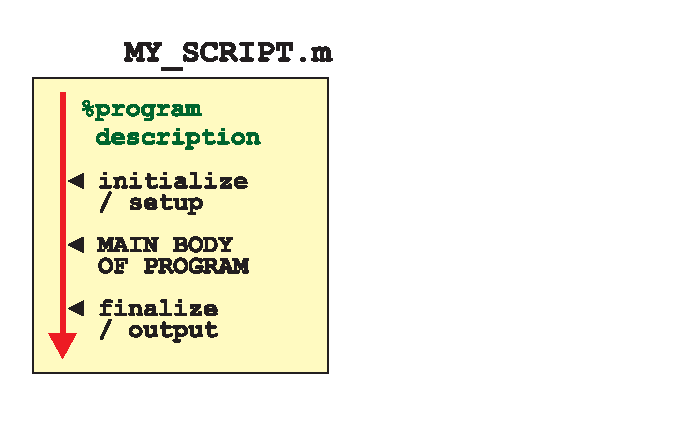
\includegraphics[width=\linewidth]{ch0-script.eps}
\caption{Schematic for a generic \textit{script}.}
\label{fig:ch0-script}
\end{marginfigure}

\begin{marginfigure}[-0.0in]
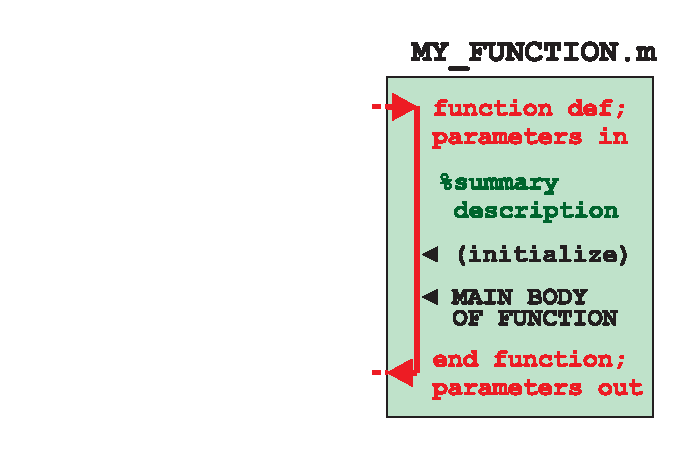
\includegraphics[width=\linewidth]{ch0-function.eps}
\caption{Schematic for a generic \textit{function}.}
\label{fig:ch0-function}
\end{marginfigure}

In these schematics, the flow (sequence) of the code is indicated by the red arrow. 

For the \textit{function}, that information is passed into the \textit{function}, and then returned back to where the function was called from, is indicated by the red arrows entering the top of the box and leaving the bottom of the box, respectively. (But note that there is no line of code at the end that tells the model to return values ... this is simply to illustrate the flow of the program, particularly when things get more complicated and there are multiple \textit{scripts} and \textit{functions} involved.)\sidenote[][0.0in]{All this should hopefully all become apparent later.}

For the \textit{script}, the code file starts with a comment (\textcolor[rgb]{0,0.501961,0}{\texttt{\%program description}}) summarizing what the \textit{script} does, although after the \textit{function} definition header line, so to should the \textit{function} (somewhere have comment lines describing what it does).

The black left-pointing filled triangles and associated text to the right, indicate categories of code content, and occurring in what order, that the programs might contain.

The purpose of these cartoons is to help you when faced with a blank page and the question: 'Where do I start' or 'What do I write' appears prominently in your mind\sidenote[][0.0in]{Also surrounded by flashing neon lights.}. It is to give you some sort of idea what bits might go where, and what general content is required in the file. The cartoons \uline{do not} (and are not intended) to show the exact details of the code content. Nor do they necessarily indicate all the different sections needed. Conversely, not all the sections illustrated may be strictly necessary and in come examples there may be nothing to 'initalize' and there may be no constants of local parameters to define the values of at the program start.

So please -- use the cartoons as a simple visual guide to the approximate structure of your program, but \uline{do not over-interpret them}.

%------------------------------------------------

\section{'Answer' codes}

For some of the more complex codes you will be expected to write, in addition to step-by-step instructions in the text, complete 'answer' codes will be provided at the back of the text. These are provided as guides to help you structure the code and see the 'bigger picture' of where all the parts fit together. The complete codes are obviously NOT provided for you simply to copy ... else you'll learn nothing. Except how to use the \textsf{CTRL-C} and \textsf{CTRL-V} key combinations.

Please use this provision as intended and for guidance only should you find yourself completely stuck.

%----------------------------------------------------------------------------------------

\mainmatter

%----------------------------------------------------------------------------------------
% CHAPTER 1
%----------------------------------------------------------------------------------------

\chapter{Elements of ... MATLAB and data visualization}
\label{ch:01}

%------------------------------------------------

\begin{fullwidth}

\newthought{Hello Newbies!} This first lab's porpoise is to start to get you familiar with what \textbf{MATLAB} 'is' and what the heck you'd actually do with it. Specifically, you are going to learn about variables and arrays and  doing some very basic/simple math in \textbf{MATLAB}, and learn how to import and manipulate (array) data in this software environment and then do some basic plotting (aka 'data visualization'). If your are clever ... you might find menu items or buttons to click that will do the same thing as typing in boring commands at the command line. In fact, you would have to be pretty dumb not to notice all that brightly colored eye-candy in the GUI (Graphical User Interface -- i.e., menus, buttons, and stuff) at the top of  the screen. However, you will get to grips with programming much quicker if you stick with the instructions and do almost everything that is asked of you using the command line  (rather than doing stuff via the GUI ), at least to start with. You'll just have to trust me for now ... We'll start with the very basics and things that you could easily do in \textbf{Excel} instead, and build up.

\newthought{Graphics} is one of the important strengths of \textbf{MATLAB}. Although other software packages and scripting languages exist that perhaps have the edge on \textbf{MATLAB} in terms of visually appealing plots and graphs, \textbf{MATLAB} is worlds apart from e.g. \textbf{Excel}. And way way better than potato printing.

\end{fullwidth}

%------------------------------------------------

\newpage

%------------------------------------------------

\section{Using the MATLAB software}

%------------------------------------------------

\subsection{Starting MATLAB}

To start with: find the \textbf{MATLAB} icon on the desktop; run the program. You should see a number of sub-windows arranged within the main \textbf{MATLAB} window, hopefully including at the very least, the \textit{Command Window}\sidenote{Conveniently labelled \texttt{Command Window} -- you cannot possibly fail to identify it ...}. Depending on whether you have used \textbf{MATLAB} before and it has remembered your settings, windows may also include: \textit{Command History}, \textit{Workspace}, \textit{Current Folder}. If instead you see; 'Tetris', 'Grand Theft Auto: San Andreas', and 'Fortnite Battle Royale', then you have the wrong software running and are going to find learning \textbf{MATLAB} rather hard. However, there is big \$\$\$ to be made in on-line gaming tournaments these days. Would you really rather be a graduate and spend the rest of your days doing a proper job?
If so, read on ...
\subsection{The command line\index{The command line}}

When \textbf{MATLAB} initially starts up, the \textit{Command Window}\index{Command Window} should display the following text: 

\begin{docspec}
        Academic License

>>
\end{docspec}

\noindent or nothing (the page is blank) ... or in order versions of the software:

\begin{docspec}
To get started, select MATLAB Help or Demos from the Help menu.

>>
\end{docspec}

\noindent Regardless, there should be a vertical blinking line (cursor) following the double 'greater than' symbols with an ocean of blank lines/space below\sidenote{Note that in nerd-speak the \texttt{>>} is called the command 'prompt' and is prompting you to type some input (Commands, swear words, etc.). See -- the computer is just sat there waiting for you to command it to go do something (stupid?). If one does not appear at the bottom of whatever is in the \textit{Command Window} is means that \textbf{MATLAB} is busy doing something extremely important. Or perhaps, \textbf{MATLAB} may have completely died. Either way, it will not accept any new/further commands until it is done calculating/dying.}.

If you are unfamiliar with using command-line driven software ... Don't Panic!\cite{Adams1979} Nothing bad can happen, regardless of what you do. Well, almost. It is possible to accidently clear \textbf{MATLAB}'s memory of the results of calculations and data processing and close plots and graphs before you have saved them, but \textbf{MATLAB} remembers all the commands you type, so in theory it is perfectly possible to quickly reproduce anything lost. (Later on we will be placing the sequence of commands into a file (that is saved) and so ultimately, \textbf{MATLAB} should turn out to be mostly fool-proof.)

To convince yourself that nothing dreadful will happen ... type ... anything. Actually 'anything' will do.

\begin{docspec}
>> anything

\textcolor{red}{Undefined function or variable 'anything'.}
\end{docspec}

Well ... not so exciting. But not so disastrous! \textbf{MATLAB} simply has no clue what you are talking about, or rather, \texttt{anything} is not a 'key word'\sidenote[][-0.25in]{i.e. a word, or sequence of characters that has a special meaning to \textbf{MATLAB} and it will act upon, as opposed to a sequence of characters that has not special meaning and \textbf{MATLAB} completely ignores.} that \textbf{MATLAB} recognises. In the specific error message, \textbf{MATLAB} could not find that \texttt{anything} was a built-in (or user-defined) \textit{function}, nor a listed \textit{variable}, both of which you'll learn about in due course.

%------------------------------------------------

\subsection{MATLAB GUI}

There are lots of fancy looking icons and pretty colors and you could spend all day staring at them and not getting any work done. Or you could learn some good programming practice. Which is why we mostly will ignore the eye-candy and little (if any) guidance will be given as to the functionality of the Graphical User Interface (\textit{GUI}). Look at this as a lesson for the user (to read the \textsf{Help}, textbook, on-line documentation, or simple go Google for an answer\sidenote{Otherwise known as Internet fishing.}).

%------------------------------------------------

\subsection{Help(!)}

If stuck at any point -- you can press the \texttt{F1} key or click on the question mark icon on the tool-bar, to bring up the indexed and searchable \textbf{MATLAB} documentation.\sidenote{It is also possible to obtain context-specific help, e.g. on a specific (built-in) \textit{function}, which we'll see in due course.}

You can also type \texttt{help} at the command line (and press the \textrm{\textsf{Return}} key).
\begin{docspec}
>> help
\end{docspec}

The result is perhaps not especially helpful. The typical usage is to provide the name of a \textit{function}\sidenote{Don't worry about what a \textit{function} is yet.} you require help on. Perversely, \texttt{help} is a function and \textbf{MATLAB} provides help on \texttt{help}. The initial output to which is as follows:
\begin{docspec}
>> help \textcolor[rgb]{1,0,1}{help}

   \textbf{help} Display help text in Command Window.
\end{docspec}

In the course text, for each \textit{function} that \textbf{MATLAB} provides a comprehensive help on, such as \docenv{help}, a simple summary version will be displayed in the right hand margin in a grey box.\sidenote{Refer to the section on 'How to use this Textbook'.}

\marginnote[-0.0in]{\begin{mdframed}[backgroundcolor=light-gray, roundcorner=10pt,leftmargin=1, rightmargin=1, innerleftmargin=5, innerrightmargin=5, innertopmargin=5,innerbottommargin=5, outerlinewidth=1, linecolor=light-gray]
\docenvdef{help}
\\Typically takes a single parameter -- the name of a \textit{function}, and returns an entirely incomprehensible description of that function and its usage at the command line.
\end{mdframed}}

%------------------------------------------------

\newpage

%------------------------------------------------

\section{Basic concepts}

%------------------------------------------------

\subsection{Variables}

A \textit{variable}\index{variable} is, in a sense, a pointer to a location in computer memory where a piece of information is stored\sidenote{In the bad old days, this pointer was the actual address in memory and might have looked something like \texttt{f04da105}.}. For instance -- open up a blank worksheet in \textbf{Excel}, and in the very top left hand cell, enter the number \textsf{10}. You can see visually, that \textbf{Excel} is referencing this location as column A, and row '1'. In fact, this location ('\textsf{A1}') is indicated in the \textsf{Name Box} to the left of the \textsf{Formula Bar}.

In \textbf{MATLAB}, a variable is associated a name to make things rather more easy and convenient. The name can be almost any sequence of characters you like, regardless of whether it is a real or fake word, as long as it does not contain numbers or special characters (e.g. \#, \$, \%, ...) or spaces. So actually, you are only left with continuous sequences of characters (otherwise knows as 'words'). Note that you can  create a variable name based on 2 (or more) real words, separated by an underscore (\texttt{\_}) if that helps describe what the \textit{variable} refers to. Valid variable names  include:

\begin{docspec}
A\\
B\\
cat\\
derpyhooves\\
this\_is\_boring\_stuff\\
BIG\\
big\sidenote{Note that \textbf{MATLAB} distinguishes between lower and UPPER case letters in a variable (i.e. \texttt{BIG} and \texttt{big} would represent two different and distinct variables). I would \uline{strongly} advise to stick to all lower case, or all upper case, to avoid possible future confusion. (or come up with a naming convention, of whatever sort (e.g. capital first letter), and stick to it.)}
\end{docspec}  

Variables are entirely useless unless they have some information assigned to them. In fact, you can type in any of the variable names above (at the command line) and \textbf{MATLAB} will deny it knows what you are talking about\sidenote[][0.25in]{Technically, \textbf{MATLAB} reports: \texttt{Undefined function or variable} which tells you it is neither a function name (more on this later), nor is defined as having any information associated with it.}.

So far so useless -- you need to \textit{assign} something to it. (The analogous situation is that when you first open an \textbf{Excel} spreadsheet and it is completely blank -- you can still reference cell A1, but there is nothing in it.) Which brings us to quite 'what' and 'how'.

First of, you need to know that variables can have the following \textit{types} of things assigned to them:

\begin{itemize}
\setlength{\itemindent}{.2in}
\item \textbf{Integer} -- An integer number is a counting number, i.e. \texttt{1, 2, 3, ...} and including zero and negative integers.
 \textbf{MATLAB} has different representations for integer numbers, depending on how large a number you need to represent (and how much memory it will need to allocated to storing it). This is something of a throw-back to the days when computers only had 1/10000000\(^{th}\) of the memory of your iPhone and were slower than half a lemon nailed to the floor. So we will not ion this text particularly worry about a numbers/computing concept called \textit{precision}.
\item \textbf{Real (floating point)}\sidenote{The distinction (sort of) is that \textit{floating point} is a specific representation of a \textbf{real} number.} -- A \textit{real} number can have a non-integer component, e.g. 1.5 or 6.022140857 \(\times\) 10\(^{23}\). Real numbers also come in different precisions in \textbf{MATLAB} (also to do with memory allocation and speed), determining not just the number of decimal places that can be represented, but also the maximum size.
\\Be aware that you can configure\footnote{Under the menu item \textsf{Preferences}.} \textbf{MATLAB} to display a particular format for real numbers, e.g.
\\\texttt{42.0}
\\versus
\\\texttt{4.2e+01}
\\(there are identical \textit{real} numbers, just a different display format).
\item \textbf{String (character)} -- One or more characters, but now allowing spaces (unlike in the case of naming \textit{variables}).
\item \textbf{Logical} -- a \textit{variable} that can be \texttt{true} or \texttt{false}\sidenote{As opposed to a Trump variable, that can have many different  alternative states of 'true', although generally, a Trump 'true' is in fact 'false'. An entire new branch of mathematics and logical deduction has been created just to process al this. } -- we'll come to quite what this means later.
\item \textbf{etc} -- No, not a real \textit{type}, but to note that \textbf{MATLAB} defines and recognises a whole bunch of other \textit{variable} \textit{types}, including \textbf{Complex} (\textbf{MATLAB} can handle \textit{complex numbers}) and \textbf{Object} (we will also not worry about \textit{objects}, which can incorporate a combination of types. At least, not yet ...). The \textbf{MATLAB} documentation contains a full list (and/or go Internet Fishing).
\end{itemize}

To come back to \textbf{Excel} -- if you select \textsf{Format Cells} (right-mouse-button-click over cell A1), you get to chose from a long list of 'formats', including \textsf{Number} and \textsf{Text}, and which have a loose correspondence with \textit{types} in \textbf{MATLAB}.

The next thing to learn is ... to ideally, not attempt to mix up (combine) variables of different \textit{types}. \textbf{MATLAB} is very forgiving when it comes to combining an \textit{integer} and a \textit{real} number in the same calculation, but in some other programming languages, this should be avoided.
However, even in \textbf{MATLAB}, \textit{strings} and \textit{reals} (or \textit{integers}) are very different things.\sidenote[][-2.5in]{Again -- in the \textbf{Excel} example, \textbf{Excel} will not let you add a \textbf{Number} and a \textbf{Text} value together, for instance. (Try it! You should see \textsf{\#VALUE!} reported.)} When necessary, different \textit{variable} \textit{types} can be converted between (see \textbf{Variable Type Conversion} Box).

\marginnote[-2.25in]{\begin{mdframed}[backgroundcolor=gray!10, roundcorner=10pt,leftmargin=1, rightmargin=1, innerleftmargin=5, innerrightmargin=5, innertopmargin=5,innerbottommargin=5, outerlinewidth=1, linecolor=gray!10]
\textbf{Variable Type Conversion}
\\\textbf{MATLAB} provides a variety of \textit{functions} (see later) for converting between different \textit{types} of \textit{variables}. The most commonly-used/useful ones are as follows:
\begin{enumerate}[noitemsep]
\item converting from a number to a \textit{string} (\texttt{s})
\begin{itemize}[noitemsep]
\item \texttt{s = num2str(N)}, where \texttt{N} is any number type variable
\item \texttt{s = int2str(I)}, where \texttt{I} is an integer
\end{itemize}
\item converting from a \textit{string} (\texttt{s}) to a number
\begin{itemize}[noitemsep]
\item \texttt{x = str2num(s)}, where \texttt{N} is (generally) a double precision (\textit{real}) number
\end{itemize}
\end{enumerate}
Case \#1 (\texttt{num2str}) is generally the most useful, e.g. in adding specific captions to plots (with caption text based on the value of a numerical variable) -- examples are given later.
\end{mdframed}}

The second and perhaps rather more important thing, is how to assign a value to a \textit{variable} (and in fact, create the variable in the first place). Programming languages such as \textbf{FORTRAN} require you to define the variable beforehand and assign it a \textit{type}.\sidenote{Partially true. An Alternative Fact of sorts.} \textbf{MATLAB} allows you to define and assign a value to a \textit{variable} all at the same time, and it will kindly work out the correct \textit{type} based on the value you assign to it.

You assign a value to a \textit{variable} using the \textit{assignment operator} \docenvdef{=}\sidenote{This is NOT 'equals' in \textbf{MATLAB}. Or any sane programming language. We will see the \textit{equality operator} shortly. \docenv{=} assigns the value or variable on its right, to the variable on the left.}. For example:
\begin{docspec}
A = 10
\end{docspec}
\noindent will assign the value \texttt{10} to the variable \texttt{A}. If you type this at the command line, \textbf{MATLAB} will kindly repeat what you have just told it and report the value of \texttt{A} back to you directly under the line you typed the command in at:
\begin{docspec}
A =

    10
\end{docspec}
\noindent Note that you do not need to add a space before and/or after the assignment operator (\docenv{=}). This is something of a personal programming and aesthetics preference, i.e. whether to pad things out with spaces or not. (Chose what you feel happiest with and later on, whatever leads to the fewest programming mistakes ...) i.e. 

\begin{docspec}
A = 10
\end{docspec}

\noindent is interpreted exactly the same as:

\begin{docspec}
A=10
\end{docspec}

Pause ... this is sort of fundamental (to using \textbf{MATLAB}), what you have just done here. It is the equivalent of typing '10' into the cell A1 in Excel (assuming we can equate the \textbf{Excel} location \textsf{A1} with the \textbf{MATLAB} variable \texttt{A}). In doing this, you have both: (a) created a variable \texttt{A}, and (b) assigned it a value of \texttt{10}.

\textbf{MATLAB} will also report in the \textsf{Workspace} window, the name and value, \textit{type} (unhelpfully called \textit{Class}), etc of all your current \textit{variables} (just one currently?). Actually, it is not all quite so simple. If you take a look at the \textit{Class} of the \textit{variable} \texttt{A} in the display window -- it is  listed as \textit{double} (a \textit{real} number) rather than an \textit{integer}. So by default, if \textbf{MATLAB} does not know what you really want, it defines \texttt{A} as a double precision real number\sidenote{If you genuinely wanted an integer, there are ways to do this, such as using a type conversion function form \textit{real} to \textit{integer} (see above).}.

Pausing again ... if you want to remind yourself of the \textit{variables} that you (or a program) have created -- you can refer to the \textsf{Workspace} window.\sidenote{There is a command line command for listing current variables (\texttt{whos}), but lets not bother with it.} Also listed here as noted above, is its value (and \textit{type} etc). Another way to access the value of a \textit{variable}, is to simply type in its name at the command line:

\begin{docspec}
>> A
\end{docspec}

\noindent and \textbf{MATLAB} will parrot back:

\begin{docspec}
A =

    10
\end{docspec}

The next complication comes when assigning a \textit{string} (a sequence of characters) to a \textit{variable}. For example, try:

\begin{docspec}
B = apple
\end{docspec}

\noindent and \textbf{MATLAB} is far from happy. As it turns out,  a sequence of characters  can also refer to a \textit{function}\sidenote{You will see \textit{functions} shortly. For now -- note that they are 'special' (reserved) words that perform some action and hence cannot also be used for a variable name.} in \textbf{MATLAB}, and this is what \textbf{MATLAB} looks for (i.e. a match to \texttt{apple} in the list or variable (and function) names). In other words, \textbf{MATLAB} does not know whether you intend \texttt{apple} to be a \textit{string} or a \textit{function}. It assumes \textit{function} ... but cannot find one with that name and then gives up. To delineate \texttt{apple} as a \textit{string}, you need to encase it in (single\sidenote{Double \texttt{""} quotation marks will not work.}) quotation marks:

\begin{docspec}
B = 'apple'
\end{docspec}

Just as \textbf{MATLAB} creates new \textit{variables} on the fly, you can re-assigned values to an existing \textit{variable}, even if this means changing the \textit{type}, e.g.

\begin{docspec}
A = 'banana'
\end{docspec}

\noindent has now replaced the real number \texttt{10} with the character string \textsf{banana} in variable \texttt{A}. This is reflected in the updated variable list details given in the \textsf{Workspace} window (and the variable \textit{Class} is now listed as \texttt{char}).\sidenote{Equally in \textbf{Excel}, you can simply type over a pre-existing value to replace it. e.g. you could type \textsf{banana} over the contents of cell \textsf{A1} (that previous held the number\textsf{ 10).}}

Finally, it is possible to suppress output to the \textsf{Command Window} when making \textit{variable} \textit{assignments} -- simply add a semi-colon (\docenvdef{;}) to the end of the \textit{assignment} statement\sidenote{Again -- your personal choice as to whether to include spaces or not between the \texttt{C}, \texttt{=}, \texttt{'banana'}, and \texttt{;} (Maybe try it both ways to convince yourself at least in this context, spaces do not matter.)}, i.e.

\begin{docspec}
C = 'banana';
\end{docspec}

\noindent Now, nothing   is echoed back to the command line but the \textsf{Workspace} is still updated to reflect this \textit{variable} \textit{assignment}. 

%------------------------------------------------

\subsection{Numerical expressions and Arithmetic operators}

You can do normal maths in \textbf{MATLAB}. Or at least, something that looks at least a little intuitive. (In fact, I often use \textbf{MATLAB} as a calculator.)
The primary/common numerical expressions are:

\begin{itemize}[noitemsep]
\setlength{\itemindent}{.2in}
\item \docenvdef{exponentiation} --- \(^{\wedge}\) --- raises one number of variable to the power of a second, e.g. a\(^{b}\), a to the power b, which is written in \textbf{MATLAB} as \texttt{a\(^{\wedge}\)b}.
\item \docenvdef{multiplication} --- \(\times\) --- e.g. a\(\times\)b, written in \textbf{MATLAB} as \texttt{a\(\ast\)b}.
\item \docenvdef{division} --- \texttt{/} --- (written as you would expect).\sidenote{Entertainingly, it turns out that if you write the reverse, backslash character (\texttt{\textbackslash}) in the equation, you divide the over way (i.e. denominator divided by numerator).}
\item \docenvdef{addition} --- \texttt{+} --- (guess).
\item \docenvdef{subtraction} --- \texttt{-} --- again, obvious/intuitive.
\end{itemize}

Technically, these symbols are called (arithmetic) \textit{operators}.

The order in which the arithmetic \textit{operators} are written down is important and will execute them in a specific order (operators higher up the list, executed first), i.e. first \texttt{\textasciicircum}, then \texttt{\(\ast\)} and\texttt{/} (equally), and last, \texttt{+} and \texttt{-} (equally). There is also \textit{negation}, when you change the sign of a \textit{variable}, and which is executed  immediately after exponentiation. e.g. 

\begin{docspec}
B = -A
\end{docspec}

\noindent The assignment operator (\docenv{=})\sidenote{This is \textbf{NOT} 'equals to'.} comes last.

\uline{If you are unclear about the order numerical operators are carried out, then place parentheses \texttt{()} around the component of the calculation you wish to be carried out first to enforce a particular order} (this can also help in making an equation easier to read and ultimately, easier to debug code). For example, consider:

\begin{docspec}
A = 3;\\
B = 6;\\
C = 2;\\
D = C*(A/B+1)\\
E = C*A/(B+1)\\
F = C*A/B+1\\
G = A*C/B+1
\end{docspec}  

\noindent Try these out (and make up your own combinations) and confirm that the answers are what you would expect them to be.

%------------------------------------------------

\subsection{Relational and logical operators}

We will see more of \textit{relational and logical operators} later when we start to get into some proper coding. For now, you only need to know that a \textit{relational operator} is one of:

\begin{itemize}[noitemsep]
\setlength{\itemindent}{.2in}
\item \docenvdef{greater than} --- MATLAB symbol \(>\)
\item \docenvdef{less than} --- MATLAB symbol \(<\)
\item \docenvdef{greater than or equal to} --- MATLAB symbol \(>\)=
\item \docenvdef{less than or equal to} --- MATLAB symbol \(<\)=
\item \docenvdef{equality} --- MATLAB symbol ==
\item \docenvdef{inequality} --- MATLAB symbol \(\sim\)=
\end{itemize}

\noindent and  test the relationship between 2 variables.

\uline{Note that the \docenv{equality} symbol (that tests the equivalence between two variables) is represented by TWO \texttt{=} characters\texttt{ (==), }and remember that a single \texttt{=} character is the \textit{assignment operator}.}

In everyday language, the answer to any one of these relational tests would be a 'yes' or a 'no'. But in \textbf{MATLAB} (and  other computer languages), the answer is given as the binary (logical) equivalent where 'yes' is represented by \texttt{1} and 'no' by \texttt{0}. You can also use \texttt{true} (\texttt{1}) and \texttt{false} (\texttt{0}), e.g. \texttt{A = true} returns:

\begin{docspec}
A =
\\ \ \ \ \ 1
\end{docspec}  

Finally, the \textit{logical operators} (again, more on this later) are:

\begin{itemize}[noitemsep]
\setlength{\itemindent}{.2in}
\item \docenvdef{or} --- symbol \texttt{||}
\item \docenvdef{and} --- symbol \texttt{\&\&}
\item \docenvdef{not} --- symbol \texttt{\(\sim\)}
\end{itemize}

For now -- simply keep mind the existence of \textit{relational and logical operators} and what they look like and we'll look into them some more later.

%---------------------------------------------
%
\subsection{Functions (built-in)}

\textbf{MATLAB} provides numerous built-in \textit{functions}\sidenote{We will be constructing our own later, at which point it should become apparent that there is nothing particular special about them.}. These \textit{functions} have specific names assigned to them, so care needs to be take not to give a \textit{variable} the same name as a \textit{function} to avoid getting confused further down the road. Giving an exhaustive list (and brief description) is outside the scope of this text\sidenote{A full list of functions can be found in the \textbf{MATLAB} Help Documentation under \textit{functions}.}. Common \textit{functions} will be progressively introduced as this text  progress. Note that in addition to the on-line \textsf{Help} documentation, information on how to use a \textit{function} and example uses is provided by typing \texttt{help }and then the \textit{function} name (separated by a space) at the command line.

\textbf{MATLAB} also provides several built-in mathematical \textit{constants} (saving having to define a variable with the appropriate number). This are simply \textit{variables} that have been already defined and assigned values, but which  you cannot change (hence the term 'constant'). For instance,  the value of \(\pi\), is assigned to a built-in \textit{function} with the name \docenvdef{pi}. You can access (display) its value  by typing its name at the command line:

\begin{docspec}
>> pi
\\ans =
\\ \ \ \ \ 3.1416
\end{docspec}  

In this example, the  use of the \textit{function} is rather trivial -- you need to tell the \docenv{pi} absolutely nothing, and it spits back the same thing (the value of \(\pi\)) each and every time. In most other \textit{functions}, you will find that you have to pass some information, and the return value will depend on the input. (This ... and what exactly a \textit{function} is, will all become apparent in due course ...)  
%---------------------------------------------

\subsection{Miscellaneous commands}

Related to what you have seen so far and will see soon, some useful miscellaneous commands include:

\begin{itemize}[noitemsep]
\setlength{\itemindent}{.2in}
\item \docenvdef{clear} --- Removes all variables from the workspace.
\item \docenvdef{clear all} --- (Removes all information from the workspace.) \item \docenvdef{close} --- Closes the current figure window.
\item \docenvdef{close all} --- (Closes all figure windows.)
\item \docenvdef{exit} --- Exits \textbf{MATLAB} and hence enables an additional trip to Starbucks to be made.
\end{itemize}

Note that a useful trick -- if you want to re-use a previously used command but don't want to type it in all over again, or want to issue a command very similar to a previously-used one -- is to hit the UP arrow key until the command you want appears. This can also be edited (navigate with LEFT and RIGHT arrow keys, and use \textsf{Delete} and \textsf{Backspace} keys to get rid of characters) if needs be. Hit \textsf{Enter} to make it all happen.

For example -- try assigning a value of \texttt{2.14159} to the variable \texttt{my\_pie}. Having noted your mistake\sidenote{An 'alternative' pi?}, correct it. Do this by bring back the previous command, and editing the \texttt{2} to a \texttt{3} (and hit return). If you refer to the \textsf{Workspace} window, you can see that you have indeed successfully changed the value of \texttt{my\_pie}.\sidenote{The point is that this is much quicker than typing the entire line in again. Although later, when we start to put lines of code into files rather than typing everything at the command line, fixing mistakes becomes easier.}

Note that there is also a \textsf{Command History} window that list all the previously issued commands and allows commands to be re-run by double-clicking on them. Copy-paste and re-running of single or multiple commands is also possible.

%------------------------------------------------

\newpage

%------------------------------------------------

\section{Vectors and arrays \#1}

So far, most of your \textit{variables} have all be what are known as \textit{scalars} -- i.e. single numbers (\textit{real} or \textit{integer})\sidenote{An exception are when you assigned a string, which technically is a vector (assuming multiple characters in the string)}.
One of the most powerful things about \textbf{MATLAB} is its ability to represent vectors (1D columns or rows of numbers or strings) and arrays -- 2D and higher dimensional regular grids of numbers or strings. (\textit{matrix}\sidenote{Not to be confused with the film containing bad acting by Keanu Reeves.} is the name commonly given to a 2-D array.)
 
%------------------------------------------------

\subsection{Creating vectors}

\marginnote[-0.5in]{\begin{mdframed}[backgroundcolor=light-gray, roundcorner=10pt,leftmargin=1, rightmargin=1, innerleftmargin=5, innerrightmargin=5, innertopmargin=5,innerbottommargin=5, outerlinewidth=1, linecolor=light-gray]
The \docenvdef{colon operator} can be used to much more rapidy create \textit{vectors} (as long as the elements form a simple sequence in value) as compared to typing in the list of values explicitly. There are two variants to the syntax:
\begin{docspecmargin}
A = j:k
\end{docspecmargin}
and
\begin{docspecmargin}
A = j:i:k
\end{docspecmargin}
In the first example, \texttt{j} and \texttt{k} and the minimum and maximum values in the sequence of numbers in the vector. \textbf{MATLAB} completes the sequence by assuming that the values monotonically increase and that the elements are separated by one (1.0) in value. e.g. 
\begin{docspecmargin}
>> A = 0:3
\\A =
\\ \ \ \ \     0     1     2     3
\end{docspecmargin}
Note that \textbf{MATLAB} is not inclined to let you directly create a vector of elements that decrease in value (you'll need to flip this puppy about to re-order it if that is what you want -- see later).
\\In the second example, \texttt{i} is the increment \textbf{MATLAB} will use to complete the sequence from \texttt{j} to \texttt{k}. In the example in the text, you could have created the \textit{array} \texttt{B} by typing: 
\begin{docspecmargin}
>> B = 0.5:0.5:2.5
\\B =
\\ \ \ \ \     0.5000    1.0000    1.5000    2.0000    2.5000
\end{docspecmargin}
(More commonly, you might place the \textit{colon operator} and its min/(/increment)/max values inside a pair of brackets, i.e. \texttt{A = [0:3].} so that it is unambiguous that you are creating an \textit{array}
\end{mdframed}}

\textit{Vectors} are 1-D arrangements of numbers (or characters or \textit{strings}).  You can enter them into \textbf{MATLAB} as a list of space-separated value, encased in (square) brackets, \texttt{[ ]}, e.g. 

\begin{docspec}
B = [0.5 1.0 1.5 2.0 2.5]
\end{docspec}

\noindent or with the value comma-separated:
 
\begin{docspec}
B = [0.5, 1.0, 1.5, 2.0, 2.5]
\end{docspec}

Either way, you end up with a \textit{vector} on its side as a single row of numbers which in math-speak would look like:

\begin{docspec}
\(B=\)
\(\begin{pmatrix}0.5 & 1.0 & 1.5 & 2.0 & 2.5 \\
\end{pmatrix}\)
\end{docspec}

You can also create the equivalent, upright orientated \textit{vector} (as a single column of numbers) by separating the elements by a semi-colon:

\begin{docspec}
C = [0.5; 1.0; 1.5; 2.0; 2.5]
\end{docspec}

\noindent which gives the maths-speak representation:
 
\begin{docspec}
\(C=\)
\(\begin{pmatrix}0.5 \\
1.0 \\
1.5 \\
2.0 \\
2.5 \\
\end{pmatrix}\)
\end{docspec}

You might ponder on (or even try out) how you would create equivalent arrangements of numbers in an \texttt{Excel} sheet. From here on, it will rapidly become apparent why you would \uline{not} want to be doing all this in \textbf{Excel}, although it remains a presumably familiar place to start from and makes links to the weirdness of \textbf{MATLAB} from.\sidenote{As such, I encourage you to still think in \textbf{Excel} world as far as possible for a little while yet, because I think it will help get to grips with \textbf{MATLAB} array notation more quickly. And indeed, \textbf{MATLAB} has a very \textbf{Excel}-like array editor window to help bridge the gap.}

%------------------------------------------------

\subsection{Basic vector manipulation}

There are several basic and very useful ways of manipulating \textit{vectors} (and as we'll see later -- \textit{matrices}). To start with, you might want to determine the  orientation and length of a \textit{vector}. There are several different ways to go about this, which in order of grown-up-ness are:

\begin{enumerate}[noitemsep]
\setlength{\itemindent}{.2in}
\item Display the contents of the \textit{vector} in the command window by typing its name at the \textsf{command line}. Obviously, this will quickly become useless for very large \textit{vectors}\sidenote[][-1.0in]{Try creating a \textit{vector} from 1 to 100,000 and assign it to a \textit{variable}. Refer to the use of the \docenv{color operator} (see earlier).
\\You will find that adding a semicolon to the end of the line to suppress output and instead viewing the vector in the \textsf{Workspace Window}.}.
\item Refer to the \textsf{Workspace window}, -- initially, the contents of the vector are displayed (under column \textsf{Value}) and you have to count, but after a certain point, the size (and not contents) of the \textit{vector} is displayed.
\item Use the \docenv{length} or \docenv{size} function (see Box). 
\item Refer to the \textsf{Workspace window} ... but ... by default, the \textsf{Size} of variables is not one of the displayed columns (instead, it has to be added from \textsf{Choose Columns} right-mouse-button-click menu item)\sidenote[][-1.25in]{Although as per above -- the size is displayed under \textsf{Value} for a sufficiently large \textit{vector}.}. 
\end{enumerate}

\marginnote[-1.0in]{\begin{mdframed}[backgroundcolor=light-gray, roundcorner=10pt,leftmargin=1, rightmargin=1, innerleftmargin=5, innerrightmargin=5, innertopmargin=5,innerbottommargin=5, outerlinewidth=1, linecolor=light-gray]
\docenvdef{length}
\\You can determine the length of a \textit{vector} A with ...
\begin{docspecmargin}
length(A)
\end{docspecmargin}
returning its \textit{integer} length, and which could in turn be assigned to a \textit{variable}, e.g. \texttt{B = length(A)}. (Technically, \docenv{length} returns the largest dimension of an \textit{array}.)
\end{mdframed}}

\marginnote[-0.0in]{\begin{mdframed}[backgroundcolor=light-gray, roundcorner=10pt,leftmargin=1, rightmargin=1, innerleftmargin=5, innerrightmargin=5, innertopmargin=5,innerbottommargin=5, outerlinewidth=1, linecolor=light-gray]
\docenvdef{size} (use \#1)
\\Returns both dimensions, even though for a \textit{vector}, one of them always has a value of \texttt{1}. This does allow you to determine its orientation though, as for the example of \texttt{A = [1:10]}: 
\begin{docspecmargin}
>> size(A)
\\ans =
\\ \ \ \ \ 1    10
\end{docspecmargin}
(1 row and 10 columns). For \texttt{A = A'}: 
\begin{docspecmargin}
>> size(A)
\\ans =
\\ \ \ \ \ 10    1
\end{docspecmargin}
(10 rows and 1 column).
\end{mdframed}}

If you find that you want a different orientation (row vs. column) of the a \textit{vector}, the \textit{vector} can be flipped around (converting row-to-column and column-to-row) using the \textit{transpose operator} (\texttt{.'}), e.g.:

\begin{docspec}
D = B.'
\end{docspec}

\noindent will turn the vector \texttt{B} into one (assigned to the \textit{variable} \texttt{D}) with he same orientation as \texttt{C}. \sidenote{Note ... \textbf{MATLAB} gives the syntax as \texttt{.'}, whereas I always only ever added the \texttt{'} bit ... which works ...} You can also use the \docenv{transpose operator} (see Box).

You can also re-order the values in a \textit{vector} (hence addressing the restriction in using the \textit{colon operator} to create a \textit{vector} that the values must be monotonically increasing rather than decreasing). Depending on the orientation of the \textit{vector}, you can use either the \docenv{flipud} (for column \textit{vectors}), or \docenv{fliplr} (for row \textit{vectors}) \textit{functions} to re-order the elements.

\marginnote[-0.0in]{\begin{mdframed}[backgroundcolor=light-gray, roundcorner=10pt,leftmargin=1, rightmargin=1, innerleftmargin=5, innerrightmargin=5, innertopmargin=5,innerbottommargin=5, outerlinewidth=1, linecolor=light-gray]
\docenvdef{flipud}, \docenvdef{fliplr}
\\These two functions allow you to re-order a vector. Their use is simple:
\begin{docspecmargin}
>> B = flipud(A)
\end{docspecmargin}
will invert the order of elements of a column vector, and:
\begin{docspecmargin}
>> B = fliplr(A)
\end{docspecmargin}
will invert the order of elements of a raw vector. Simples! Lesson over.
\end{mdframed}}

%------------------------------------------------

\subsection{Addressing elements in vectors}

This next bit is maybe the single most important (and weird) part of \textbf{MATLAB}. As you go through this section (and also the later one on \textit{matrices}) -- have \textbf{Excel} open as a aid to visualize how \textbf{MALTAB} represents \textit{arrays}. Start by entering the 5 numbers, from 0.5 to 2.5, in sequential cells, working down from \textsf{A1} (this is the \textbf{MATLAB} vector \texttt{B} in the example that follows).

Values can be extracted (or read) from a vector by specifying the index (technically, this should be an \textit{integer}, but \textbf{MATLAB} is pretty forgiving and you can get away with using a \textit{real} (number) when specifying an index) of the element required (counting along, left-to-right, or top-to-bottom, depending on the \textit{vector} orientation), e.g. 

\begin{docspec}
>> B(5)
\\ans =
\\ \ \ \ \ 2.5000
\end{docspec}

\noindent or:

\begin{docspec}
>> C(3)
\\ans =
\\ \ \ \ \ 1.5000
\end{docspec}

\marginnote[-1.50in]{\begin{mdframed}[backgroundcolor=light-gray, roundcorner=10pt,leftmargin=1, rightmargin=1, innerleftmargin=5, innerrightmargin=5, innertopmargin=5,innerbottommargin=5, outerlinewidth=1, linecolor=light-gray]
The \docenvdef{transpose operator}, in \textbf{MATLAB}-speak, "\textit{returns the nonconjugate transpose of A}". Who knows what that means. In slightly more everyday (i.e. down here on Earth) language, it: "interchanges the row and column index for each element". Or sort of, just interchanges the rows and columns. The operation can be written:  
\begin{docspecmargin}
>> B = A.'
\end{docspecmargin}
or  
\begin{docspecmargin}
>> B = transpose(A)
\end{docspecmargin}
In practice, you can get away with being lazy (and in fact this is how it was in the old days, and just write):  
\begin{docspecmargin}
>> B = A'
\end{docspecmargin}
(but get into the habit of using the formally correct, \textbf{Mathworks} official and UN-approved, syntax of \texttt{.'}).
\end{mdframed}}

\noindent(In this text, I will refer to accessing a particular element (or elements) of a \textit{vector} (or \textit{array}) via its \textit{index} as addressing. Unless I forget, then I might say something else. You'll have to keep on your toes -- don't expect consistency here!)\sidenote{Recognise the parallel with \textbf{Excel} here -- the value in position \texttt{5} in the \textbf{MATLAB} vector \texttt{B}, is the same as specifying the contents of cell \textsf{A5} in \textbf{Excel}.}

There is a \textbf{MATLAB} \textit{function} \docenv{end} (see Box) that enables you to easily address (accessing via its index) the very last value in a \textit{vector} (in \textbf{MATLAB}, the \textit{index} of the first position is always \texttt{1}).

For addressing more than one element of a vector at a time, you can use the \docenv{colon operator} (see Box). \sidenote{Again -- e.g. in \textbf{Excel}, the sum of the \textsf{5} elements in column \textsf{A} (the equivalent 'vector'), would be \textsf{=SUM(A1:A5)}.}

As well as reading out an existing value of a \textit{vector}, you can also replace an existing value by assigning the new value to the appropriate \textit{index} position. e.g. to replace the first element
with a value of \texttt{0.0}:
\begin{docspec}
B(1) = 0.0
\end{docspec}

\noindent (Here, you are saying that you would like to assign the value of \texttt{0.5} to the element in the \textit{vector} given by the index \texttt{1}. The previous content of the array at \textit{index} position \texttt{1} is simply over-written.)

\marginnote[-0.50in]{\begin{mdframed}[backgroundcolor=light-gray, roundcorner=10pt,leftmargin=1, rightmargin=1, innerleftmargin=5, innerrightmargin=5, innertopmargin=5,innerbottommargin=5, outerlinewidth=1, linecolor=light-gray]
You can access more than a single element of a vector at a time, by means of the \docenv{colon operator}, \texttt{:} to define a min, max range of indices. For example:  
\begin{docspecmargin}
>> B(2:4)
\\ans =
\\   1.0000
\\   1.5000
\\   2.0000
\end{docspecmargin}
To select all elements:  
\begin{docspecmargin}
>> B(:)  
\\ans =
\\    0.5000
\\    1.0000
\\    1.5000
\\    2.0000
\\    2.5000
\end{docspecmargin}
\end{mdframed}}

\marginnote[-0.25in]{\begin{mdframed}[backgroundcolor=light-gray, roundcorner=10pt,leftmargin=1, rightmargin=1, innerleftmargin=5, innerrightmargin=5, innertopmargin=5,innerbottommargin=5, outerlinewidth=1, linecolor=light-gray]
\docenvdef{end}
\\Represents the largest index in a \textit{vector} when addressing it, or in \textbf{MATLAB}-speak: "end can ... serve as the last index in an indexing expression".
\end{mdframed}}

%------------------------------------------------

\newpage

%------------------------------------------------

\section{Basic graphing (aka. 'data visualization')}

So far ... I suspect this is heavy-going and there is a lot to try and remember, such as command names, although knowing just that certain commands exist, is enough to start with and \textbf{MATLAB} \textsf{Help} can be used later to find out the exact name (and usage syntax). All this, and we have not  even  gotten on to \textit{matrices} (2-D arrays) yet ... So, we'll take a diversion to look at some basic plotting techniques that will  make sense now that you can create \textit{vectors} of numbers to plot (and later, important some 'real' data). Unless you have forgotten how to create \textit{vectors} already ... :(

%------------------------------------------------

\subsection{Plotting}

First -- create yourself a dummy dataset to plot. You are going to need to create yourself a pair of \textit{vectors} -- these can have any values (all numbers though) in them that you like, but perhaps aim for 1 vector with values counting up from 1 to 10 (or similar) -- this will form your \textit{x}-axis, and the 2nd column ... whatever you like. \sidenote[][-3.00in]{Looking ahead -- you could create a y-axis \textit{vector} formed of the squares of the numbers in the x-axis \textit{vector}: 
\begin{docspecmargin}
>> Y = X.\(^{\wedge}\)2  
\end{docspecmargin}
(The \texttt{.\(^{\wedge}\)} bit says to square the value of each and every  element in the \textit{vector}.)}
The command \docenvdef{figure} creates a \textsf{figure window}, which is where \textbf{MATLAB} displays its graphical output ... but on its own, without anything in it ... useless. So, lets put something in it, with the simplest possible graphical way of displaying data called \docenv{plot}. 

\marginnote[-2.25in]{\begin{mdframed}[backgroundcolor=light-gray, roundcorner=10pt,leftmargin=1, rightmargin=1, innerleftmargin=5, innerrightmargin=5, innertopmargin=5,innerbottommargin=5, outerlinewidth=1, linecolor=light-gray]
\docenvdef{plot}
\\The \textbf{MATLAB} function \docenv{plot} ... plots. More specifically, it plots pairs of (x,y) data and by default, does not plot the points explicitly but joins the(x,y) locations up by straight line segments. \textbf{MATLAB} calls these a '2D line plot', although there are plotting options that allow you only to display the individual (x,y) points (making it like the \docenv{scatter} function, which we'll see later).
\\Its most basic usage is: 
\begin{docspecmargin}
plot(X,Y)
\end{docspecmargin}
where \texttt{X} and \texttt{Y} are vectors -- of the same length (\uline{important}), but not necessarily of the same orientation (i.e. if one was a row vector and one a column vector, \textbf{MATLAB} would work it out, although it is perhaps best to avoid such a situation arising).
\\There are many options that go with this function, some of which we'll see and use later. You can also input matrixes as \texttt{X} and \texttt{Y} apparently. But I have absolutely no clue as to what might happen. I suspect that the plot will end up looking like a bad acid trip. 
\end{mdframed}}

With any new \textbf{MATLAB} command (\textit{function}), get into the habit of looking up the \textsf{help} text  (also refer to alternative/simplified help provided in this text). The key information that will get you started appears at the very top of the text that \textsf{help} returns on \texttt{plot}:

\begin{docspec}
PLOT(X,Y) plots vector Y versus vector X.
\end{docspec}

\noindent This tells you that you need to pass to \texttt{plot}, your \textit{x}-axis data \textit{vector} (by its variable name), followed by your y-axis data \textit{vector} (by its variable name) -- comma separated. Do this, and depending on just what or how random your \textit{y}-axis data was, you should end up with something like Figure \ref{fig:plot-basic} in a window captioned "\texttt{Figure 1}".\sidenote{If you cannot see the figure window ... check that the window is not hidden behind the main \textbf{MATLAB} program window!} 

This ... is easily the least professional plot ever (aside from anything created in \textbf{Excel}). And one that breaks all the most basic rules of scientific presentation, such as an absence of any labelling of axes. There is also no title, although here in the course text I have added a figure caption in the document so I can sort of get away with it. This is the default output of the basic \texttt{plot} function and you'll just have to deal with it (i.e. add a series of commands to add missing elements of the \texttt{plot}).

\begin{marginfigure}[0.0in]
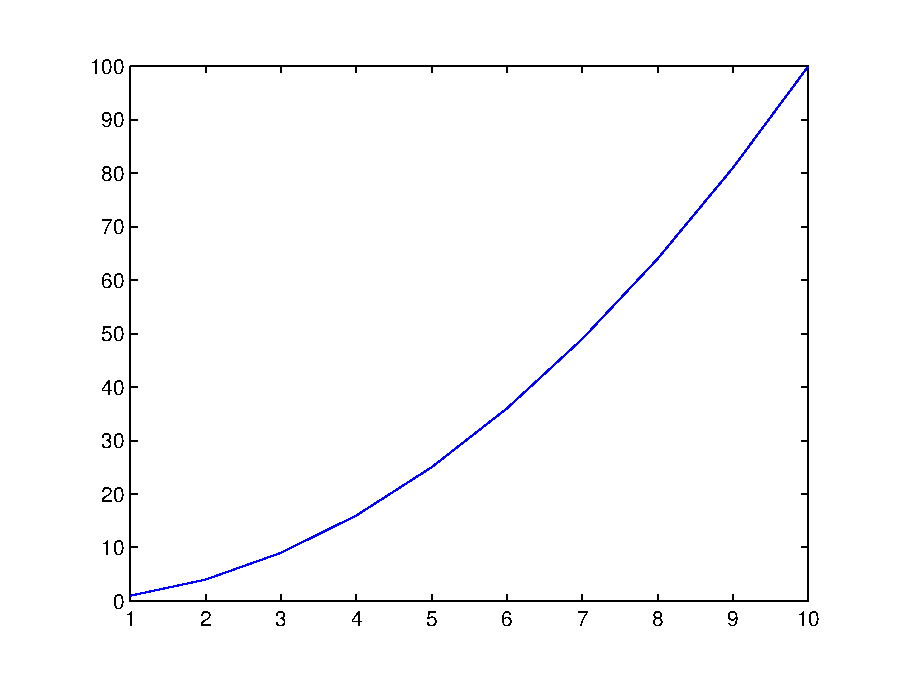
\includegraphics[width=\linewidth]{ch1-plot-basic1.eps}
\caption{Example of the default output of the \texttt{plot} function.}
\label{fig:plot-basic}
\end{marginfigure}

Note that by default, \textbf{MATLAB} also scales both axes to reasonably closely match the range of values in the two data vectors. In the example here, the default min and max
axes limits in fact turn out to be the min and max values in the \textit{x} and y-axis data because the data is composed of relatively simply/whole numbers. If however the maximum \textit{y} value was very  slightly larger, you'd see that \textbf{MATLAB} would adjust the maximum \textit{y}-axis limit to the next convenient value so as to preserve a relatively simple series of labelled tick marks in the axis scale. In fact, why not try that -- replace your maximum data value, with a value that is very slightly larger (an example is given in Figure \ref{fig:ch1-plot-basic3}).
\sidenote[][-0.75in]{If you have created a dummy dataset in which the value in the last row is the largest, replacing it is simple -- remember the use of \texttt{end} in addressing an element in an array. If your dataset does not monotonically increase and the largest value falls somewhere in the middle ... you could cheat' and open the array in the variable editor and discover which row it occurs on.} Then re-plot and note how it has changed (if at all -- it will depend somewhat on what data you invented in the first place).

\begin{marginfigure}[0.0in]
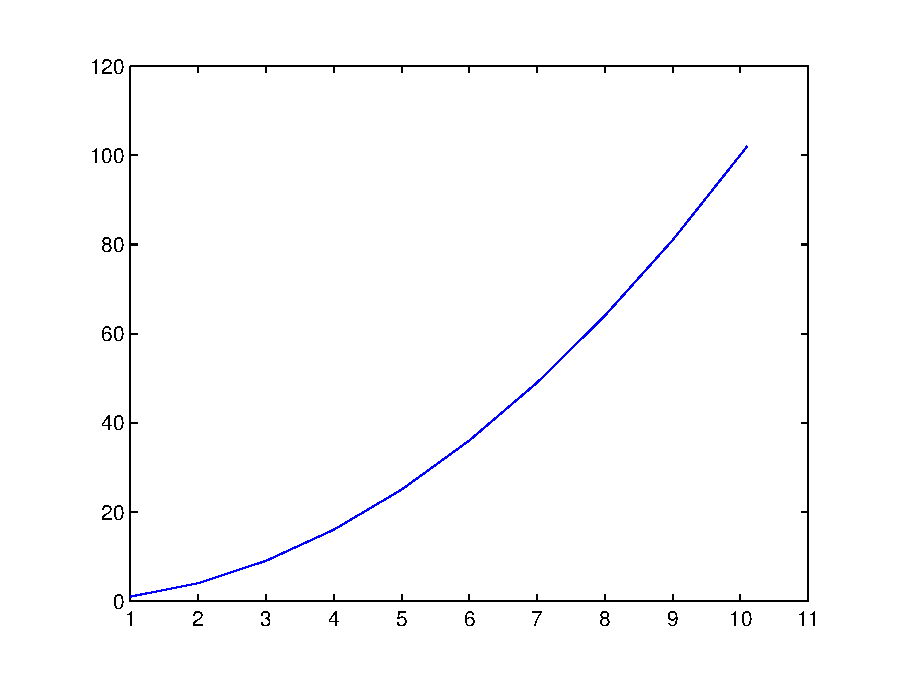
\includegraphics[width=\linewidth]{ch1-plot-basic3.eps}
\caption{A plot illustrating axis auto-scaling (maximum \textit{x} and \textit{y} values now slightly larger than 10 and 100, respectively).}
\label{fig:ch1-plot-basic3}
\end{marginfigure}

%------------------------------------------------

\subsection{Graph labelling}

You have two options for editing the figure and e.g. adding axis labels. Firstly, you can use the \textit{GUI} and the series of menu items and icons at the top of the \textsf{Figure window} to manipulate the figure. I suspect you'll prefer this ... but it is not very flexible, or rather, it requires your input each and every time you want to make changes or additions to a figure. The second possibility is to issue a series of \textbf{MATLAB} commands at the \textsf{command line}. (The advantage with the latter we'll see later when we introduce \docenvdef{m-files}.) For now, I'll illustrate a few basic commands:

\begin{marginfigure}[0.0in]
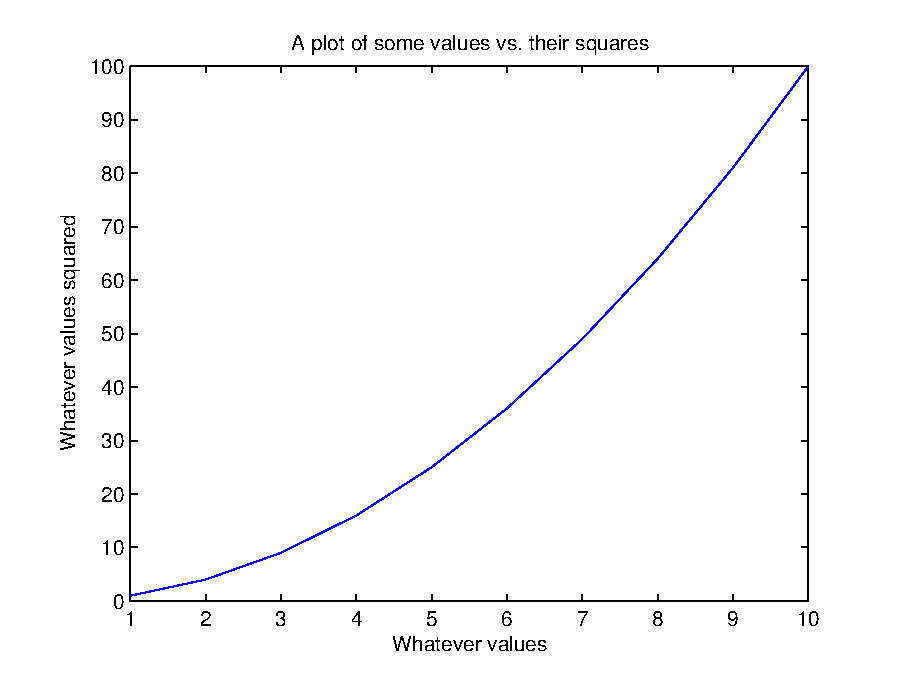
\includegraphics[width=\linewidth]{ch1-plot-basic2.eps}
\caption{A (only very slightly) improved plot.}
\label{fig:ch1-plot-basic2}
\end{marginfigure}

\begin{enumerate}[noitemsep]
\setlength{\itemindent}{.2in}
\item The first, obvious thing to do is to add axis labels. The commands are simple -- \docenvdef{xlabel} and \docenvdef{ylabel}. They each take a string as an input, which is the text you would like to appear on the axis.
If you change your mind, simply re-issue the command with the text you would like instead.
\item The command for title, perhaps unsurprisingly, is \docenvdef{title}. Again, pass the test you would like to appear as a string (in inverted commas \texttt{''}), or pass a the name of variable that contains a string (no \texttt{'}' then needed).
\item You might want to specify the axis limits. The command is \docenv{axis} and it takes a vector of 4 values as its input -- in order: minimum x, maximum x, minimum y, and maximum y value. e.g. \texttt{axis([0 10 -100 100])} would specify an \textit{x}-axis running from 0 to 10, and a \textit{y}-axis from -100 to 100.
\end{enumerate}

Information as to how to use all of these commands can be found via \textbf{MATLAB} \texttt{help}. But a typical sequence, that gives rise to the improved plot shown in Figure \ref{fig:ch1-plot-basic2}, is given in the margin.

\marginnote[-1.0in]{\begin{mdframed}[backgroundcolor=light-gray, roundcorner=10pt,leftmargin=1, rightmargin=1, innerleftmargin=5, innerrightmargin=5, innertopmargin=5,innerbottommargin=5, outerlinewidth=1, linecolor=light-gray]
Example of adding axis labels and a plot title ...
\begin{docspecmargin}
>> xlabel ... 
\\ \ \ ('Whatever values');
\\>> ylabel ...
\\ \ \ ('Whatever values ... squared');
\\>> title ...
\\ \ \ ('A plot of some ...
\\ \ \ values vs. their ... 
\\ \ \ squares');   
\end{docspecmargin}
\end{mdframed}}

Note that in the usage of all the above listed commands, they all require something to be passed within a set of parentheses -- \texttt{( )}. In fact, they are all \textbf{MATLAB} functions and require an input (hence the use of the parentheses). Some of the functions require a \textit{string} input, such as the name of the title in \docenv{title}, and this must be encased in quotation marks -- \texttt{' '} to designate it a string rather than a \textit{variable} name.\sidenote{You could instead assign a \textit{string} to a \textit{variable}, and then pass the \textit{variable} name (no quotation marks).}

%------------------------------------------------

\subsection{Sub-plots}

You can also have more than one plot in a single \textsf{Figure window}. As an example, create some sine waves using the \docenvdef{sin} function (see \texttt{help}) over the range 0 < \textit{x} < 2\(\pi\), e.g.:
\begin{docspec}
>> x = 0:0.1:2*pi;
\\>> y = sin(x);
\\>> y2 = sin(2*x);
\end{docspec}
(Note how in the first line, the \textit{colon operator} is used to create an \textit{x} vector from 0 to 2\(\pi\), in steps of 0.1. The second and third lines calculate the sine of all the x values, and sine of 2 times the \textit{x} values, respectively, and assign the results to a pair of new vectors, \texttt{y} and \texttt{y2}.)

\marginnote[-2.0in]{\begin{mdframed}[backgroundcolor=gray!10, roundcorner=10pt,leftmargin=1, rightmargin=1, innerleftmargin=5, innerrightmargin=5, innertopmargin=5,innerbottommargin=5, outerlinewidth=1, linecolor=light-gray]
\docenvdef{axis}
\\For once, helpfully, \textbf{MATLAB} says:
\\"\textit{\texttt{axis([xmin xmax ymin ymax])} sets the limits for the x- and y-axis of the current axes.}"
\\\noindent which is about all you need to know (other than the minimum and maximum limits along the \textit{x-axis} are represented by \texttt{xmin}, \texttt{xmax}, and the minimum and maximum limits along the \textit{y-axis} are \texttt{ymin}, \texttt{ymax}).
\end{mdframed}}

To place several different plots on the same figure uses the \docenvdef{subplot} command \sidenote{>> help subplot}. The \docenv{subplot} command is used as: \texttt{subplot(m,n,p)} where \texttt{m} is the number of rows of plots you want to have in your figure, \texttt{n} is the number of columns of plots in your figure, and \texttt{p} is the index of the plot you wish to create (see: Figure \ref{fig:ch1-subplot}).  

\begin{marginfigure}[0.0in]
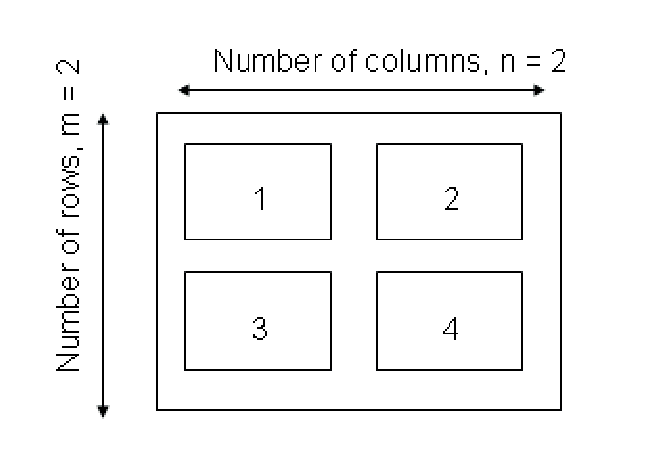
\includegraphics[width=\linewidth]{ch1-subplot.eps}
\caption{Arrangement of subplots.}
\label{fig:ch1-subplot}
\end{marginfigure} 

The basic code then goes something like:
\begin{docspec}
>> figure(1);
\\>> subplot(2,2,1);
\\>> plot(x,y);
\\>> subplot(2,2,2);
\\>> plot(x,y2);
\\>> subplot(2,2,3);
\\>> plot(x,-y);
\\>> subplot(2,2,4);
\\>> plot(x,-y2);
\end{docspec}

\noindent In this case, the 3rd and 4th subplots simply display the inverse of the curves in the subplots above. 

%------------------------------------------------

\subsection{Saving graphics and figures}

You might just want to save the figure. (Why create it in the first place in fact if you are just going to throw it away ... ?) Again, you can do this via the \textit{GUI} or at the \textit{command line}
\sidenote[][-0.25in]{
To export a graphic at the command line, use the \docenvdef{print} function. To cut a long story short (see: \texttt{help print}), to print to a postscript file:
\\\texttt{print('-dpsc2', FILENAME)}
\\\noindent where \texttt{FILENAME} is the filename as a \textit{string} or a \textit{variable} containing a \textit{string}.
}.
From the \textit{GUI}, you have the option to save the figure in a way that can be loaded later and re-edited -- this is the \texttt{.fig} format option. Or you can save (export) in a variety of common graphics formats (although once saved in this format, the graphics can only be edited later using a graphics package).

You can also close \textsf{figure windows} (see Box). No seriously. They are not forever. ;)

\marginnote[-0.50in]{\begin{mdframed}[backgroundcolor=light-gray, roundcorner=10pt,leftmargin=1, rightmargin=1, innerleftmargin=5, innerrightmargin=5, innertopmargin=5,innerbottommargin=5, outerlinewidth=1, linecolor=light-gray]
To close the current (active) \textsf{Figure window}, the command is:
\\ \texttt{>> close}
\\ \noindent To close all currently open \textsf{Figure windows}:
\\ \texttt{>> close all}
\end{mdframed}}

%------------------------------------------------

\newpage

%------------------------------------------------

\section{Vectors and arrays \#2}

A \textit{matrix} is another special case of an \textit{array} -- this time 2-D (rather than 1-D in the case of a vector). \textbf{MATLAB} totally hearts them.
 
\subsection{Creating matrices and arrays}

You can enter \textit{matrices} (2-D arrays) into \textbf{MATLAB} in several different ways:

\begin{enumerate}[noitemsep]
\setlength{\itemindent}{.2in}
\item Enter an explicit list of elements.
To enter the elements of a \textit{matrix}, there are only a few basic conventions:
\begin{itemize}[noitemsep]
\setlength{\itemindent}{.4in}
\item Separate the elements of a row with blanks or commas.
\item Use a semicolon, \texttt{;} , to indicate the end of each row.
\item Surround the entire list of elements with  brackets, \texttt{[ ]}.
\end{itemize}
\item Load matrices from external data files.
\item Generate matrices using built-in functions.
\end{enumerate}

\newthought{As an example}, type in the following at the command prompt:
\begin{docspec}
A = [15 7 11 6; 13 1 6 10; 21 17 5 3; 5 15 20 9]
\end{docspec}
\noindent \textbf{MATLAB} then displays the matrix you just entered\sidenote{Remember that you can add an \texttt{;} to the end of the line to prevent the results of the \textit{variable} assignment being displayed in the \textsf{Command Window}.}:
\begin{docspec}
A =\\
\ \ \ \ 15   7  11   6\\
\ \ \ \ 13   1   6  10\\
\ \ \ \ 21  17   5   3\\
\ \ \ \ 5   15  20   9
\end{docspec}

In math-speak, this would be equivalent to:

\vspace{2mm}
\(A=\begin{pmatrix}15 & 7 & 11 & 6 \\
13 & 1 & 6 & 10 \\
21 & 17 & 5 & 3 \\
5 & 15 & 20 & 9 \\
\end{pmatrix}\)
\vspace{2mm}

\noindent Once you have entered the \textit{matrix}, it is automatically remembered in the \textbf{MATLAB} workspace. You can refer to it simply as \texttt{A}.

Now go find the \textit{array} you have just created in the \textsf{Workspace window}. Double-click on its name icon and see what goodies appear on the screen. This is a fancy \textit{array} editor which looks a bit like one of those dreadful \textbf{Excel} spreadsheet things. You can see that this might be handy to edit, view, and keep track of at least moderate quantities of data. This is a useful facility to have. However, we are going to concentrate on the command-line operation of \textbf{MATLAB} in this class because that will give you far more power and flexibility in applying numerical techniques to problem solving, and will form the basis of \textit{scripting} (computer programming by another name) that we will see in a few lectures time. Close down this nice toy to leave just the original windows.

Elements in the \textit{matrix} can be addressed using the syntax:
\begin{docspec}
A(i,j)
\end{docspec}
where \texttt{i} is the row number, and \texttt{j} is the column number. It is very very easy to keep forgetting in which order the rows and columns are indexed., but I'll tell you here and now before I forget:
\hfill \break
\\{\LARGE rows, columns}
\hfill \break
\\\noindent(You can always create a test \textit{matrix} and access a specific element to check if in doubt!)
In the example above:
\begin{docspec}
>> A(1,3)
\\ans =
\\ \ \ \ \ 11
\end{docspec}
\noindent (i.e. the value of the element in the 1st row, 3rd column, is \texttt{11}).

In general, the same \textit{functions} and \textit{operators} that applied to \textit{vectors} and you saw earlier, also apply to \textit{matrixes} (or specific dimensions of matrices).

\marginnote[-0.0in]{\begin{mdframed}[backgroundcolor=light-gray, roundcorner=10pt,leftmargin=1, rightmargin=1, innerleftmargin=5, innerrightmargin=5, innertopmargin=5,innerbottommargin=5, outerlinewidth=1, linecolor=light-gray]
Similarly as for vectors, you can access more than a single element of a matrix by means of the \docenv{colon operator}, \texttt{:}. For example: \\\texttt{A(:,1)} -- selects the 1st column
\\\texttt{A(3,:)} -- selects the 3rd row
\\\texttt{A(2:3,2:3)} -- selects the 2\(\times\)2 matrix of values lying in the centre of \texttt{A}, while \texttt{A(1:2,:)} selects the top half (first 2 rows) of the matrix.
\end{mdframed}}

Finally -- a fundamental way of accessing data that you need to learn and be familiar with, is to employ the \textit{colon operator} to select specific columns (or rows) of data. You'll find that this skill  ends up inherent to many of your attempts to process and graph data. For instance, if your (\textit{x},\textit{y}) data to plot ended up in \textbf{MATLAB} workspace in matrix form (it very commonly does) rather than as 2 sperate vectors (as you had when you first plotted anything), you will need to select separately the \textit{x} (e.g. 1st column) data, and the \textit{y} (2nd column) data, and pass these to the \texttt{plot} function.
For the example of matrix A above, all the first column data can be selected by typing \texttt{A(:,1)}\sidenote{Remembering the HUGE hint above in 100 pt font as to the order of rows and columns ...}, which says all the rows (\texttt{:}) in the first column. Similarly, all the 2nd column data alone can be selected by \texttt{A(:,2)}. (You'll practice this endlessly later on and hopefully get it!)


\marginnote[-0.25in]{\begin{mdframed}[backgroundcolor=light-gray, roundcorner=10pt,leftmargin=1, rightmargin=1, innerleftmargin=5, innerrightmargin=5, innertopmargin=5,innerbottommargin=5, outerlinewidth=1, linecolor=light-gray]
You can also determine the shape of your \textit{array} using the \docenvdef{size} function. For a 2D \textit{array} (\textit{matrix}), when you pass it the name of your array, it returns the number of rows followed by the number of columns (in that order). 
\end{mdframed}}

%------------------------------------------------

\subsection{Basic matrix manipulation}

You can treat \textit{vectors} and \textit{matrices} (or parts of \textit{vectors} and \textit{matrices}), mathematically, as you would treat single values (i.e. \textit{scalars}) but unlike a \textit{scalar}, the transformation is applied to all specified elements of the \textit{array}. This applies for all the basic \textit{arithmetic operators}\sidenote{Technically ... or at least to be consistent with other operations, you might write multiplication as \texttt{.*} rather than just plain old \texttt{*}. The preceding dot tells \textbf{MATLAB} not to treat this as matrix multiplication but to carry out the operation on each element in turn. In this case, it is the same thing (and both notations work the same), but later, is not. (This will make more sense when you get to see it in action, later.)}. For example, for \textit{vector} \texttt{B} in the earlier example,
\begin{docspec}
>> 2*B
\\ans =
\\ \ \ \ \ 0     2     3     4     5
\end{docspec}
and
\begin{docspec}
>> B-1.5
\\ans =
\\ \ \ \ \ -1.5000   -0.5000         0    0.5000    1.0000
\end{docspec}

\newthought{Question:} Multiply all the elements of \texttt{A} by the number \texttt{17}. Assign the answer to a 3rd array (\texttt{C}). What is the value of the element \texttt{C(2,3)}? How would you ask for the 4th row, 2nd column element of the array \texttt{C}, and what is its value?

\newthought{Question:} What is the sum of the 4th column of \texttt{C}
\marginnote[-0.75in]{\begin{mdframed}[backgroundcolor=light-gray, roundcorner=10pt,leftmargin=1, rightmargin=1, innerleftmargin=5, innerrightmargin=5, innertopmargin=5,innerbottommargin=5, outerlinewidth=1, linecolor=light-gray]
The \textit{function} \docenvdef{sum} ... sums things. The \textbf{MATLAB} Help documentation (\texttt{help sum}) says:
\\'\texttt{If A is a vector, sum(A) returns the sum of the elements.}'
\\'\texttt{If A is a matrix, sum(A) treats the columns of A as vectors, returning a row vector of the sums of each column.}'
\end{mdframed}}
? (Sure -- you also do it by using a calculator, but you will not always have such a small data-set as here. Perhaps you'll get a much larger data-set in the assessed exercise ;) So, practice doing it properly.) The \textbf{MATLAB} function for this is \docenv{sum}.

\newthought{Question:} What is the sum of the 2nd row of \texttt{C}?
 For a \textit{matrix} (rather than a \textit{vector}) as input, \docenv{sum}  returns the individual sums of each column, and so on its own;
\begin{docspec}
>> C\\
C =\\
\ \ \ \ 255   119   187   102\\
\ \ \ \ 221    17   102   170\\
\ \ \ \ 357   289    85    51\\
\ \ \ \ 85   255   340   153\\
\vspace{2mm}

>> sum(C)\\
ans =\\
\ \ \ \ 918   680   714   476\\
\end{docspec}
\noindent gives you a row \textit{vector} consisting of the sums of the individual columns of the \textit{matrix} \texttt{C} above.

This is where the \docenv{transpose} function (\texttt{'}) comes in handy (see earlier). In this case, it flips a (2D) \textit{matrix} around its leading diagonal (columns become rows, and rows, columns)\sidenote[][-1.0in]{This is almost true. Technically the function you want is \texttt{.'}, as \texttt{'} will change the sign of any imaginary components. For real numbers, they are the same.}
\marginnote{\begin{mdframed}[backgroundcolor=light-gray, roundcorner=10pt,leftmargin=1, rightmargin=1, innerleftmargin=5, innerrightmargin=5, innertopmargin=5,innerbottommargin=5, outerlinewidth=1, linecolor=light-gray]
In addition to \docenv{transpose}, other useful array manipulation functions include:
\\\noindent \docenv{flipup} -- flips the matrix in the up/down direction
\\\noindent \docenv{fliplr} -- flips the matrix in the left/right direction
\\\noindent \docenvdef{rotate} -- rotates the matrix
\\\noindent(As always, refer to the \texttt{help} on specific functions.)
\end{mdframed}}.
\begin{docspec}
>> C'\\
ans =\\
\ \ \ \ 255   221   357    85\\
\ \ \ \ 119    17   289   255\\
\ \ \ \ 187   102    85   340\\
\ \ \ \ 102   170    51   153
\end{docspec}
\noindent (transposing the \textit{matrix} turns the rows into columns)
\begin{docspec}
>> sum(C')\\
ans =\\
\ \ \ \ 663   510   782   833
\end{docspec}
\noindent Now you get a row \textit{vector} consisting of the sums of the individual columns of the \textit{matrix} C, but since you have transposed the \textit{matrix} \texttt{C} first, these four values are actually equal to the row sums.

Finally, you could transpose the answer:
\begin{docspec}
>> sum(C')'\\
ans = \\
\ \ \ \ 663\\
\ \ \ \ 510\\
\ \ \ \ 782\\
\ \ \ \ 833
\end{docspec}
\noindent to give you  a row \textit{vector} format that corresponds to the rows  of the original \textit{matrix} \texttt{C}.
\sidenote[][-0.25in]{Note how you can combine multiple \textit{functions} in the same statement to create \texttt{sum(C')'}. However, to start with, it is much safer to do each step separately and hence be sure what you are doing.}

Finally, if you wanted the sum of *all* the elements in the \textit{matrix} \texttt{C} in the example above, you could sum all the columns to give you a row \textit{vector} of partial sums, and then sum the elements in the row \textit{vector} to give you the grant total sum of all the elements. You can do this, either in completely separate steps\sidenote{In general in programming -- use as many smaller, separate steps as you like and are most comfortable. The more you break down the calculation, the clearer it will be to you and the easier to debug if things go wrong. However, this does come at the expense of longer and longer code and sometimes more compact code is easier to deal with.}:
\begin{docspec}
>> D = sum(C);\\
>> E = sum(D);
\end{docspec}
or all in one go:
\begin{docspec}
>> F = sum(sum(C));
\end{docspec}

It does not matter if you sum the column of \texttt{C} first, or the row first -- maybe test this to satisfy yourself that this is true.

%------------------------------------------------

\subsection{Some matrix math :(}

We will not concern ourselves overly with multiplying \textit{vectors} and \textit{matrices} together ... but you should be aware that \textbf{MATLAB} can do matrix math. For now, it is worth nothing the difference between \texttt{*} and \texttt{.*} operators in the context of arrays. For example, consider 2 vectors, \texttt{A} and \texttt{B}:

\begin{docspec}
>> A = [1 1 2 2];\\
>> B = [1 2 3 4];
\end{docspec}

To multiple the elements of \texttt{A} and \texttt{B} together \uline{pair-wise}, use .*:

\begin{docspec}
>> C = A.*B
\\
C =\\
\ \ \ \ 1     2     6     8
\end{docspec}

Without the dot, you get the vector product ... well, you would if the \textit{vectors} were in an appropriate orientation, i.e.:

\vspace{1mm}
\(\begin{pmatrix}1 & 1 & 2 & 2 \\
\end{pmatrix}\times\begin{pmatrix}1 \\
2 \\
3 \\
4 \\
\end{pmatrix}\)
\vspace{1mm}

\noindent which you get by typing:

\begin{docspec}
>> C = A*B'
\\
C =\\
\ \ \ \ 17
\end{docspec}
(which is  calculated from: \(1\times1 + 1\times2 + 2\times3 + 2\times4\)).

An example of the equivalent matrix usage is:

\begin{docspec}
>> D = [1 1; 2 2];\\
>> E = [1 2; 3 4];
\end{docspec}

The pair-wise multiplication of each element of the 1st matrix with the corresponding element of the 2nd matrix is:
\begin{docspec}
>> F = E.*E
\\
F =\\
\ \ \ \ 1     4\\
\ \ \ \ 9    16
\end{docspec}

In contrast, for matrix multiplication, written in math-speak as:

\vspace{2mm}
\(\begin{pmatrix}1 & 1 \\
2 & 2 \\
\end{pmatrix}\times\begin{pmatrix}1 & 2 \\
3 & 4 \\
\end{pmatrix}\)
\vspace{2mm}

we would write:

\begin{docspec}
>> F = E*E
\\
F =\\
\ \ \ \  7    10\\
\ \ \ \ 15    22
\end{docspec}

If your matrix math is rusty and you are not following this, maybe refresh it (your memory of basic matrix math).

%------------------------------------------------

\newpage

%------------------------------------------------

\section{Loading and saving data}

There are a number of different ways to load/import data into the \textbf{MATLAB} \textsf{Workspace}. Rather than try and tediously list and describe the commands and syntax and blah blah, we'll be going through a couple of (hopefully) slightly less tedious data-based examples as we progress through the course text. In this way, if nothing else, you might accidently learn some science even if nothing much about \textbf{MATLAB} ...

%------------------------------------------------

\subsection{Where am I?}

Before anything -- you need to know 'where you are'. If the file you want to load in is not in the directory \textbf{MATLAB} is using, it will not find it. And if you save something and have no idea where it is being saved ... that can hardly go well.

\textbf{MATLAB} has a default directory that it starts up in and looks at first. For basic Windoz installations\sidenote[][-1.0in]{At installation, this directory can be specified and hence may not be this one. Also -- different operating systems will have different default locations.} of the software, this directory is:

\begin{docspec}
C:\textbackslash Users\textbackslash mushroom\textbackslash Documents\textbackslash MATLAB
\end{docspec}

\noindent So, where the \docenv{load} command requires a filename to be passed, you will need to enter either the full location of the file; i.e., starting with the drive letter (e.g. as per displayed in the \textsf{Windows Filemanger} address bar), or the relative path to where the file is located.

\marginnote[-1.75in]{\begin{mdframed}[backgroundcolor=light-gray, roundcorner=10pt,leftmargin=1, rightmargin=1, innerleftmargin=5, innerrightmargin=5, innertopmargin=5,innerbottommargin=5, outerlinewidth=1, linecolor=light-gray]
\docenvdef{load}
\\Loads variable from a file into the workspace. The syntax is:
\begin{docspecmargin}
>> load(FILENAME)
\end{docspecmargin}
where \texttt{FILEMANE} is the name of the file (remember: \texttt{FILEMANE} needs to be a string and enclosed in quotation marks, OR, a variable that points to a string.
\\ The file might be plain text (ASCII) or a \textbf{MATLAB} workspace file (see below). To force \textbf{MATLAB} to treat the file input as ASCII or a \textbf{MATLAB} workspace file, pass a second parameter (separated from the filename by a comma) -- \texttt{'-ascii'} for ascii, and \texttt{'-mat'} for a \textbf{MATLAB} workspace file. 
\\Note that in loading an ASCII data file, any line starting with a \texttt{\%} is ignored. Also note that the data \uline{must} be in a column format with no missing data.
\\ For an ASCII file, the name of the variable created to hold the data being imported is automatically generated. So in the example of the data file being called \texttt{'twilight.txt'}, the variable generated will be called \texttt{twilight}. You can instead chose to assign the imported data to a variable name of your choice, by e.g.: 
\begin{docspecmargin}
>> sparkle = load('twilight.txt','-ascii');
\end{docspecmargin}
(all one line)
\end{mdframed}}

It is not necessarily to have all your files end up here, so there is a way to change the \textbf{MATLAB} directory that you are working in which work in a similar way to \textbf{UNIX}/\textbf{LINUX} for those of you who are familiar with navigating your way around these operating systems. You can change the directory that \textbf{MATLAB} is  working from by typing:
\begin{docspec}
>> cd DIRECTORY\_PATH
\end{docspec}
where \texttt{DIRECTORY\_PATH} is the path to the directory in which you want to work from and where you want your data files (and later, code files) to live. Foe example, if (in \textbf{Windoz}) you have mounted a USB drive, it might be assigned drive letter \textsf{E:}. To change \textbf{MATLAB}'s working directory to this drive, you would type:
\begin{docspec}
>> cd E:
\end{docspec}
If, you have a directory \textsf{working} on the USB drive, you could change \textbf{MATLAB}'s working directory by:
\begin{docspec}
>> cd E:\textbackslash working
\end{docspec}

Note that an alternative format (syntax) for \texttt{cd} is as a \textit{function}, e.g,
\begin{docspec}
>> cd('E:\textbackslash working')
\end{docspec}

with the directory path passed as a string.

Another alternative is to add a 'search path' (\texttt{addpath}) so that \textbf{MATLAB} knows of an additional place to look for files.  For example:
\begin{docspec}
>> addpath('E:\textbackslash working')
\end{docspec}
would keep your current working directory unchanged, but tell \textbf{MATLAB} to also look in the directory \textsf{E:\textbackslash} for files.

\marginnote[-1.0in]{\begin{mdframed}[backgroundcolor=light-gray, roundcorner=10pt,leftmargin=1, rightmargin=1, innerleftmargin=5, innerrightmargin=5, innertopmargin=5,innerbottommargin=5, outerlinewidth=1, linecolor=light-gray]{
\docenvdef{addpath}
\\The command \docenv{addpath} will add a search path to the \textbf{MATLAB} workspace. The syntax is:
\\\texttt{addpath(DIRECTORY\_PATH)}
\\where \texttt{DIRECTORY\_PATH} is a \textit{string} (characters in between inverted commas) or name of a variable containing a string.}
\end{mdframed}}

There is also, of course, the GUI -- from the \texttt{File} menu the option \texttt{Import Data..}. will run the data import Wizard -- note that you might have to select \texttt{All Files (*.*)} from the file type option box in order to find the file. I'll leave you to work the rest out for yourselves ... Maybe try importing the data into \textbf{MATLAB} this way once you have done it successfully using the \docenv{load} function at the command line. The \textit{GUI} can also be used to change the directory you are working from (duplicating the functionality of the \texttt{cd} command) and add paths to search (duplicating the functionality of the \texttt{addpath} command).

In summary: go with whatever works best for you in terms of working directory. Easiest might be simply to work directly from a directory on your USB pen-drive (and e.g. have a named different directory for each week of class).  

%------------------------------------------------

\subsection{Loading and importing data}

The simplest way (other than via the \textbf{MATLAB} \textit{GUI} and the beautiful green \textsf{Import Data} icon) is to use the \docenv{load} function (see Box)\sidenote{There is also a much more flexible way of loading text-based data using the function \texttt{textscan}, but that also requires files to be explicitly opened and closed using \docenvdef{fprintf}. We'll see a little of this later.}.

As a brief exercise and practice using \texttt{load} -- first download the data file \texttt{etheridge\_etal\_1996.txt} from the course webpage\sidenote{\texttt{http://www.seao2.info/teaching.html}}. You might start by viewing the contents of the file by opening it in any text viewer (or \textbf{Excel}\sidenote{In fact, you could even try first plotting it in \textbf{Excel}.}). This is always a good place to start as it enables you to see what you are getting yourself in to (i.e. format of the file, any potential formatting issues, approximate size and complexity of the dataset, etc).

Now, import the data into the \textbf{MATLAB} workspace using the  \texttt{load} command. Because the data is a plain text (ASCII) format and not a special \textbf{MATLAB} \textsf{.mat} file, you need to specify the format as '\texttt{ascii}' when usingn the \texttt{load} command (see box or \textsf{help}):

\begin{docspec}
>> load('etheridge\_etal\_1996.txt','-ascii');
\end{docspec}

If you tell \textbf{MATLAB} nothing different, it will create a variable for you containing the file content, with the variable name based on the filename (minus the extension). If you prefer a different variable name, then simply pass the results of the load command -- the contents of your file -- to a different \textit{variable}, e.g.

\begin{docspec}
>> mydata = load('etheridge\_etal\_1996.txt','-ascii');
\end{docspec}

\noindent instead assigns the \texttt{load}-ed data to the \textit{variable} \texttt{mydata}.

Try  typing the name of the \textit{variable} that was automatically created (\texttt{etheridge\_etal\_1996}) (or the one you chose if you assigned the imported data to a specific variable name  as per detailed in the Box) to provide a crude view of the data. To view the contents of the \textit{variable} in the \textsf{Variables window} -- double  click on the name of the \textit{variable} in the \textbf{MATLAB} \textsf{Workspace window.} This should open up a spreadsheet-like window in which the data can be viewed, sorted, and even edited.

For practice, try plotting the data\sidenote[][-2.0in]{using \texttt{plot}} and remembering to label the figure appropriately\sidenote[][-1.75in]{ FYI: the first column of the data and x-axis is year, and the 2nd column of the data and y-axis is the mixing ratio of CO\(_{2}\) in air in units of ppm.}. \uline{However} ... remember, the format of the \textbf{MATLAB} \texttt{plot} function is:

\begin{docspec}
plot(X,Y) plots vector Y versus vector X
\end{docspec}

\noindent So you need to specify each column of the data (i.e. each \textit{vector}) separately and explicitly.\footnote[][-2.0in]{If you just type \texttt{plot} and pass the (here: default) name of the data array: 
\begin{docspecmargin}
>> plot(etheridge\_etal\_1996);
\end{docspecmargin}
... strange ... things are happening (as per Figure \ref{fig:ch1-plot-icecore_default}). In fact, \textbf{MATLAB} is doing what \textbf{Excel} would in a \textsf{Line Chart} with 2 columns of data selected -- rather than plot y (2nd column) vs. x (1st column), the values of both columns are plotted against row number. Which is why you should remember to use the \textsf{Scatter} (or \textsf{(X,Y)}) \textsf{Chart} in \textbf{Excel} for plotting (x,y) data.}

\begin{marginfigure}[-0.0in]
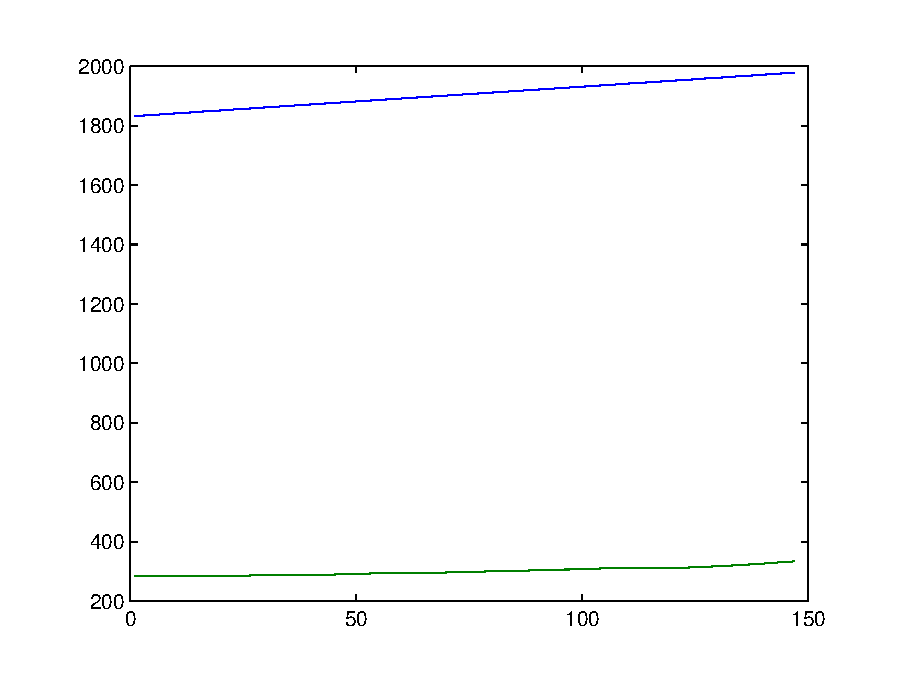
\includegraphics[width=\linewidth]{ch1-plot-icecore_default.eps}
\caption{Result of simply throwing the entire data matrix at \texttt{plot} ....}
\label{fig:ch1-plot-icecore_default}
\end{marginfigure}

You can do this step-by-step, and create yourself 2 vectors, one for the x-values and one for the y-values, and then \texttt{plot}:

\begin{docspec}
>> X = etheridge\_etal\_1996(:,1);\\
>> Y = etheridge\_etal\_1996(:,2);\\
>> plot(X,Y);
\end{docspec}

Or go straight for the kill:

\begin{docspec}
>> plot(etheridge\_etal\_1996(:,1),etheridge\_etal\_1996(:,2));
\end{docspec}

Breaking things down like  is an equally valid way of doing things. It is longer ... taking 3 lines rather than 1, but the most important thing is to be happy that you understand what is going on. If breaking things down into multiple lines and creating new \textit{variables} helps -- \uline{DO IT}! Ultimately, you should end up with something like Figure \ref{fig:ch1-plot-icecore}.

\begin{marginfigure}[-0.0in]
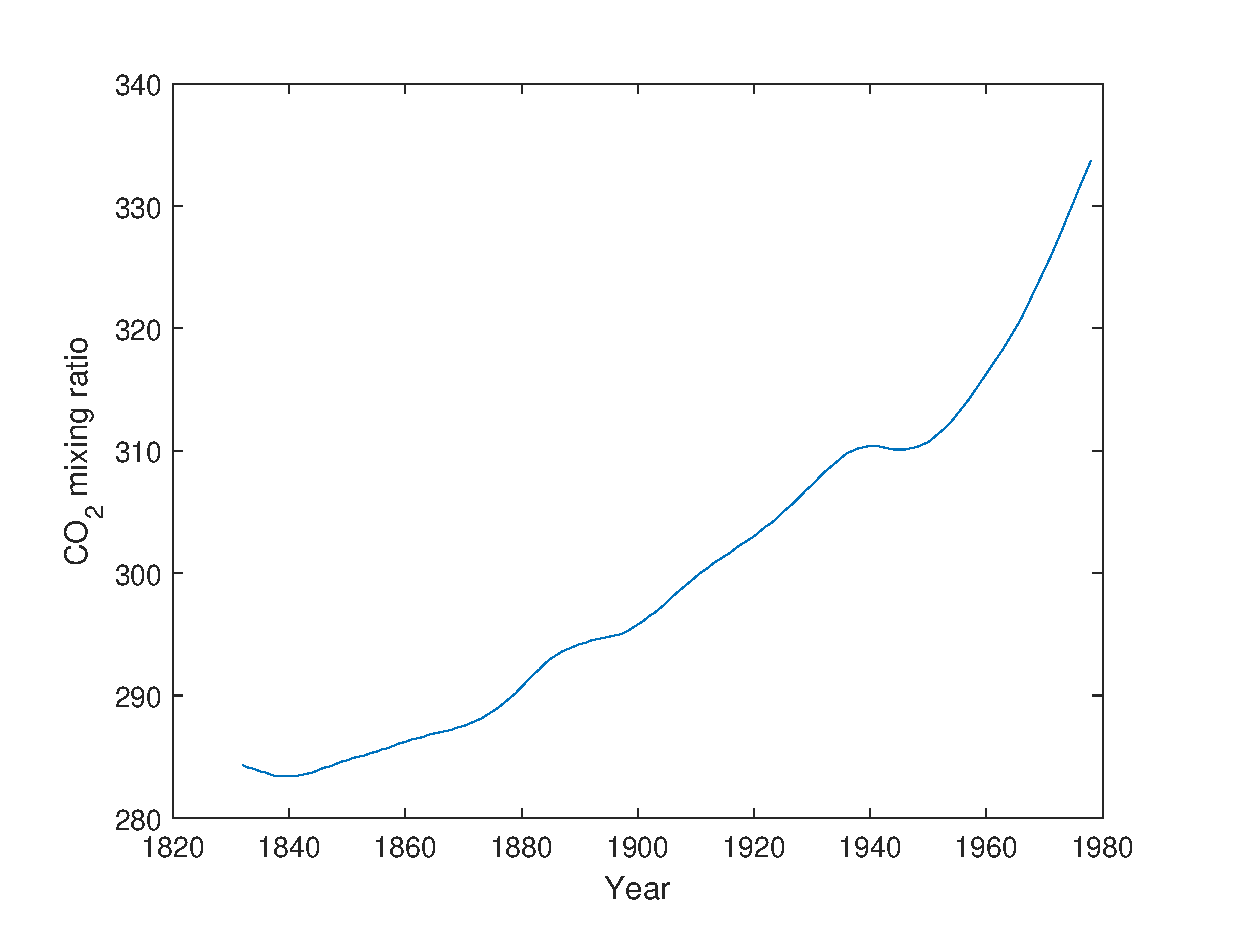
\includegraphics[width=\linewidth]{ch1-plot-icecore.eps}
\caption{Spline fit to measured changes in CO2 concentration in Law Done ice core, following \textit{Etheridge et al.} [1996].}
\label{fig:ch1-plot-icecore}
\end{marginfigure}

%------------------------------------------------

\subsection{Saving and exporting data}

Specific variables can  be saved in a plain text (ASCII format) by means of the \docenv{save} function (and then re-loaded in using \docenv{load}). You have to specify that you want a text format (rather than the default \textbf{MATLAB} \textsf{.mat} workspace format) -- see Box. Try re-saving the ice-core data as an ASCII format
text file (with a new filename) ... and then load it in again.

%------------------------------------------------

\subsection{Loading and saving the workspace}

The entire workspace (including all variables and their values, or just the values in a single variable if you wish) can be saved to a file and then later re-opened. The file format is specific to the \textbf{MATLAB} program and the file-name extension by default is \docenv{.mat}. You might find this very helpful to use in long lab exercise or large modelling projects, particularly if you do not come back to work at the exact same computer each time or wish to use continue the same piece of work on a laptop elsewhere. Try saving the current \textsf{Workspace}, then close down the \textbf{MATLAB} program. Re-running it, and then loading in your saved \texttt{.mat} file.
\sidenote[][-1.00in]{This sequence is going to look something like:
\begin{docspecmargin}
>> save mystuff
\\>> exit
\end{docspecmargin}
...
\begin{docspecmargin}
load mystuff
\end{docspecmargin}
Remember that when you re-start \textbf{MATLAB} you may have to change directories, add a path (\textsf{addpath}), or provide a full path to the \texttt{.mat} file, depending on where you saved it. 
}

\marginnote[-0.00in]{\begin{mdframed}[backgroundcolor=light-gray, roundcorner=10pt,leftmargin=1, rightmargin=1, innerleftmargin=5, innerrightmargin=5, innertopmargin=5,innerbottommargin=5, outerlinewidth=1, linecolor=light-gray]
\docenvdef{save}
\\Saves variables from the workspace to a file. There are two main forms (syntaxes) of the command:
\begin{docspecmargin}
>> save(filename)
\end{docspecmargin}
which saves the entire workspace to a \textsf{.mat} file (with the filename given by the string \texttt{filename} (in quotation marks), and:
\begin{docspecmargin}
>> ...
\\ \ save(filename,A,'-ascii')
\end{docspecmargin}
saves the data in the variable \texttt{A} (which must be given as a string, i.e. also enclosed in quotation marks) in plain text (ASCII) format. 
\end{mdframed}}

\marginnote[-0.00in]{\begin{mdframed}[backgroundcolor=light-gray, roundcorner=10pt,leftmargin=1, rightmargin=1, innerleftmargin=5, innerrightmargin=5, innertopmargin=5,innerbottommargin=5, outerlinewidth=1, linecolor=light-gray]
\textbf{MATLAB}'s proprietary file format for saving the contents of your current Workspace is indicated by a \docenvdef{.mat} file name extension (in Windoz). 
\end{mdframed}}

Hopefully ... all your loaded/created variables etc. have been recovered ... ?

%------------------------------------------------

\newpage

%------------------------------------------------

\section{Basic data processing (and yet more plotting)}

This section runs through a couple of common basic data manipulation/processes techniques follow, plus some further plotting/visualization.

%------------------------------------------------

\subsection{Sorting data (in arrays)}

As an example to kick-off some data-processing tricks, load in the dataset of ('proxy') reconstructed atmospheric CO\(_{2}\) concentrations spanning the Phanerozoic: \textsf{paleo\_CO2\_data.txt}. You can just import it into \textbf{MATLAB} using the \docenv{load} function -- remember the specific syntax of load:

\begin{docspec}
>> load(FILENAME)
\end{docspec}

where your \texttt{FILENAME} is \textsf{paleo\_CO2\_data.txt} and needs to be passed to load as a string, i.e.

\begin{docspec}
>> load('paleo\_CO2\_data.txt')
\end{docspec}

If you tell \textbf{MATLAB} nothing different (and do not assign the results of the \texttt{load} function to a different \textit{variable} name), \textbf{MATLAB} will create a \textit{variable} called \texttt{ paleo\_CO2\_data} (see \textsf{Workspace}).

If you view the contents of the variable\texttt{ paleo\_CO2\_data} (or whatever you might have passed the \texttt{load}-ed data to), you will see that there is a slight complication  -- unlike the ice core CO2 dataset, you now have 4 columns in this array\sidenote{Remember that you can diagnose its size with ... \texttt{size} (or refer to the Workspace window)}. The first column is age (Ma), the second the mean CO\(_{2}\) value, while the 3d and 4th columns are the low and high, respectively, uncertainty limits of the CO\(_{2}\) value.

Recalling how to reference specific columns of data in a matrix\sidenote{HINT: the \texttt{colon operator} (see earlier).}, and either referencing the columns of the array directly, or creating yourself separate vectors \texttt{X} and \texttt{Y} (see earlier) -- plot the mean paleo CO\(_{2}\) value as a function of age (in Ma). If you  closed the previous \textsf{Figure} window (see earlier), it is not essential to explicitly open one (using the \texttt{Figure} command) -- when you use the \texttt{plot} command, if there is no open \textsf{Figure} window, \textbf{MATLAB} will kindly open one for you. How thoughtful. The result should be something like \ref{fig:plot-CO2basic}.

O dear ...

\begin{marginfigure}[0.0in]
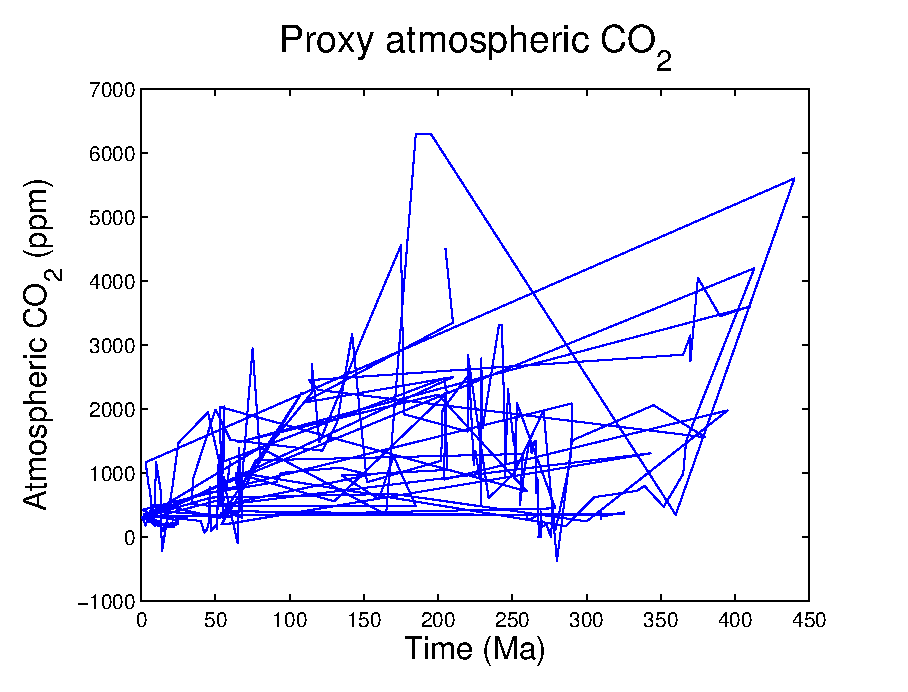
\includegraphics[width=\linewidth]{plot-CO2basic.eps}
\caption{proxy reconstructed past variability in atmospheric CO2.}
\label{fig:plot-CO2basic}
\end{marginfigure}

So ... that was not so successful. What is happening in the default behaviour of \texttt{plot}, is that the location defined by each subsequent row of data is being joined to the previous one with a line. This was fine for the ice-core CO2 example dataset because time progressed monotonically  in the first column, e.g. the data was ordered as a function of time. If you view the paleo CO\(_{2}\) data, this is not the case and time (age in Myr) does not progress monotonically in an always-getting-older (or always-getting younger) fashion.\footnote{In fact, in the original, full version of the data, ordering is by proxy type first, and then study citation, and only then age ...}

Your options are then:

\begin{enumerate}[noitemsep]
\setlength{\itemindent}{.2in}
\item You could import the data into \textbf{Excel}, then re-order (sort) it, then export it, then re-load it ...
\item You could sort it in \textbf{MATLAB} using the \textit{GUI} variable view window. But lets not cheat for now.
\item You could sort it in \textbf{MATLAB} at the command line. How? Well, a reasonable gamble, which actually turns out to be a total win, is to try:
\begin{docspec}
>> help sort
\end{docspec}
However, reading the \textsf{help} text carefully (and you can always try it out and see what exactly it does if you are not sure), \docenv{sort} will sort all columns independently of each other, whereas we want the first column sorted and the remaining columns linked to this order. So this is not the \textit{function} that you are looking for.
\end{enumerate}

This is where it is worth paying attention to the bottom of \textbf{MATLAB} \textsf{help} and the \textsf{\uline{see also}} section. In this case, \textbf{MATLAB}\ lists \docenv{sortrows} as a possibility. The \textsf{help} text on this looks a little more promising. It is still slightly opaque (so also see Box), so the best thing to do is to try it (and view the results)! 

\begin{docspec}
>> ordered\_data = sortrows(paleo\_CO2\_data)
\end{docspec}

\noindent where the result of sorting the rows (of all columns) I have assigned to the variable \texttt{ordered\_data}. If you now try plotting this, e.g.

\begin{docspec}
>> plot(sorted\_data(:,1),sorted\_data(:,2));
\end{docspec}

\noindent it looks rather better -- Figure \ref{fig:plot-CO2basic2}. (This is a good illustration of a guess of a \textit{function} that was not quite what was needed, but following up on the \texttt{help} suggestions leads to a more appropriate \textit{function}.) At least now the curve is reminiscent of past changes in global temperature and the geological Wilson cycle, with high \(CO_{2}\) values in the Cretaceous and Jurassic and then lower again in the Carboniferous (roughly matching the progression of ice and hot house (and then back to recent ice ages) climates).

\marginnote[-2.25in]{\begin{mdframed}[backgroundcolor=light-gray, roundcorner=10pt,leftmargin=1, rightmargin=1, innerleftmargin=5, innerrightmargin=5, innertopmargin=5,innerbottommargin=5, outerlinewidth=1, linecolor=light-gray]
\docenvdef{sortrows}
\\In its simplest usage: 
\begin{docspecmargin}
>> B = sortrows(A)
\end{docspecmargin}
... "sorts the rows of a matrix in ascending order based on the elements in the first column. When the first column contains repeated elements, \texttt{sortrows} sorts according to the next column and repeats this behavior for succeeding equal values."
\\So, if the first column of the matrix was time, the data would be sorted into ascending time.
\end{mdframed}}

\begin{marginfigure}[0.0in]
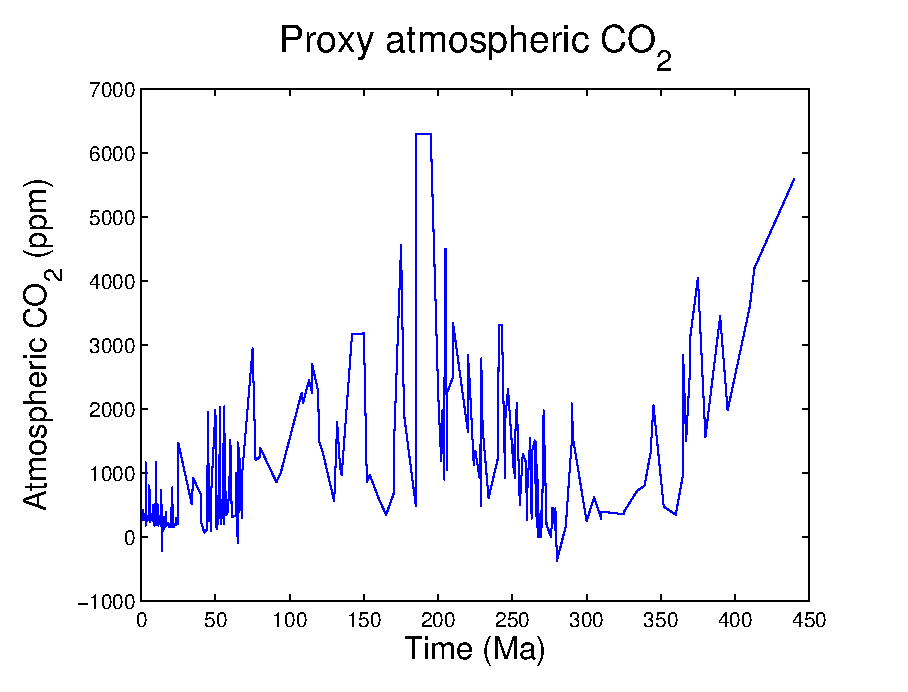
\includegraphics[width=\linewidth]{plot-CO2basic2.eps}
\caption{Proxy reconstructed past variability in atmospheric CO2 (sorted data).}
\label{fig:plot-CO2basic2}
\end{marginfigure}

A little later you will meet an alternative plotting \textit{function} that does not require the data to be sorted into any sort of order. But you should note that you can also use \docenv{plot}, but omitting the line segments by specifying only a symbol, e.g.

\begin{docspec}
plot(x,y,'ro');
\end{docspec}

\noindent (here, plotting circles for the data points in red) so that it does not matter in which order the individual points are plotted (and the same result is obtain from both sorted and un-sorted data).

%------------------------------------------------

\subsection{Data scaling}

\noindent As an example practicing some basic data scaling: download the historical global temperature anomaly dataset\sidenote[][-0.0in]{\href{https://www.ncdc.noaa.gov/cag/global/time-series/globe/land\_ocean/ytd/12/1880-2017/\#https://climate.nasa.gov/vital-signs/global-temperature/}{NOAA}}:

\vspace{1mm} \noindent \textsf{temperature\_globalanom.txt} \vspace{1mm}

The columns are: (1) year , (2) annual mean ocean+land surface temperature \uline{anomaly} (i.e. temperature change relate to some reference value, where here is the observed 1901-2000 mean). Remember, you can \texttt{load} and assign data to an easier-to remember variable by e.g.:

\begin{docspec}
>> data1 = load('temperature\_globalanom.txt','-ascii');
\end{docspec}

Plot the annual mean temperature anomaly for the full range of years, as per Figure \ref{fig:ch1-plot-temperature1}. (plus labels, title, etc etc).

\begin{marginfigure}[0.0in]
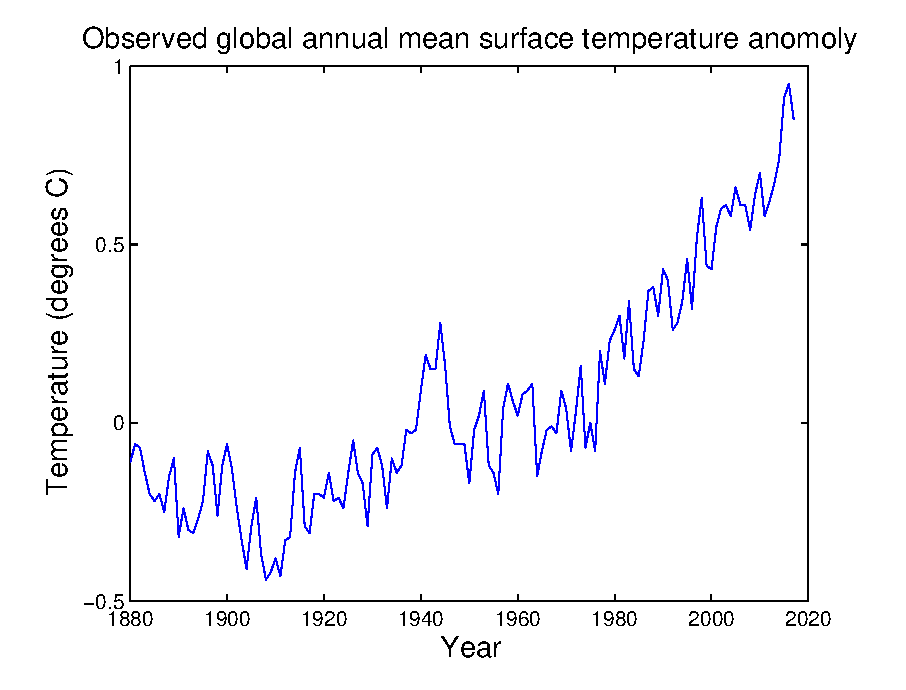
\includegraphics[width=\linewidth]{ch1-plot-temperature1.eps}
\caption{Observed annual global mean surface temperature anomaly (compared to year 1910 to 2000 average).}
\label{fig:ch1-plot-temperature1}
\end{marginfigure}

The 20th century average global temperature across land and ocean surface areas is apparently 13.9\degree C. So first, change the temperature anomaly data into absolute temperatures -- you'll do this by by adding the 20th century global average value, 13.9, to all the data values (the second column of your array).\sidenote[][-0.0in]{Remember -- you can increase the value of every element in an array, by simply adding that number, e.g. if \texttt{A} is you array of data, and \texttt{B} is a \textit{scalar} (the value you want to increase all array values by);
\begin{docspecmargin}
>> C = A + B;
\end{docspecmargin}
will have the effect of adding \texttt{B} to ever element in \texttt{A}, and assigning to a new array, \texttt{C}. Or alternatively, you can replace the contents of array \texttt{A} with the new values:
\begin{docspecmargin}
>> A = A + B;
\end{docspecmargin}
In your specific example:
\begin{docspecmargin}
>> data1(:,2) = ... 
\\data1(:,2) + 13.9
\end{docspecmargin}
(all one line) will have the effect of taking the 2nd column of the array \texttt{data1}, adding 13.9 to all the values, and writing the new values back into the 2nd column of the array \texttt{data1}.
}

Now re-plot.

Next, convert the temperature units from \degree C to \degree F. An approximate conversion is:

\vspace{2mm}
\(T_{(\degree F)} = 1.8\times T_{(\degree C)} + 32 \)
\vspace{2mm}

\noindent where \(T_{(\degree F)}\) is the (new) temperature in \degree F, and \(T_{(\degree C)}\) the (old) temperature in \degree C.

For this, you will need to take your data (which is the 2nd column of the array), e.g. \texttt{data1(:,2)}, multiple by 1.8 as per the equation (\texttt{1.8*data1(:,2)}) and then add 32 (\texttt{1.8*data1(:,2) + 32})\footnote{If you have any doubts as to the order in which the operators are applied, add a set of parentheses, e.g. \\ \texttt{(1.8*data1(:,2)) + 32}}. And ... assign the results of this to a new vector or array. Or you can replace the original column (if you are feeling confident), e.g.

\begin{docspec}
>> data1(:,2) = 1.8*data1(:,2) + 32;
\end{docspec}
 
\noindent The aim is to obtain a data array in \textbf{MATLAB}, with year as the first column (year, as per the original data) and the 2nd  column as annual mean  temperature in units of \degree F.

If it helps -- play  the data conversion game in \textbf{Excel} first (e.g. creating new columns in a spreadsheet to firstly hold  absolute temperatures rather than anomalies, and then temperatures in \degree F rather than \degree C). Also if it helps -- create a new array with the modified temperature units data in (rather than replacing the 2nd column of  the original array, \texttt{data}). You can also do the conversion in 2 stages -- multiplying the (absolute) temperature (\degree C) by \(1.8\) first (perhaps creating a new array to hold this in), then adding \(32\).

Re-plot (in \textbf{MATLAB}) once again the final temperature trends in \degree F. This should look like Figure \ref{fig:ch1-plot-temperature3}.

\begin{marginfigure}[0.0in]
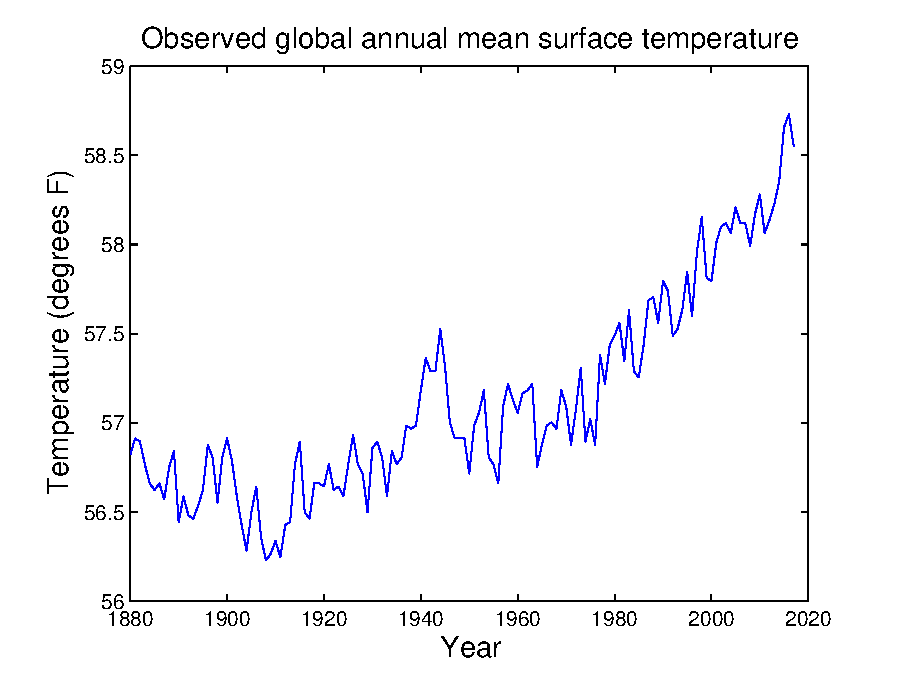
\includegraphics[width=\linewidth]{ch1-plot-temperature3.eps}
\caption{Observed annual global mean surface temperature.}
\label{fig:ch1-plot-temperature3}
\end{marginfigure}

%------------------------------------------------

\subsection{Data (row) deletion}

\noindent For some practice in data filtering (row deletion) and a little further data manipulation and graphing: download the historical temperature dataset for Riverside\sidenote[][-0.0in]{\href{https://www.ncdc.noaa.gov/cag/global/time-series/globe/land\_ocean/ytd/12/1880-2017/\#https://climate.nasa.gov/vital-signs/global-temperature/}{NOAA}}:

\vspace{1mm} \noindent \textsf{temperature\_riverside.txt} \vspace{1mm}

If you view the data file in a text editor or import into \textbf{Excel}, you can read the column headers and find out what the different columns of data are (I am not telling you!). Note that the (1st) line of the file containing the column header labels starts with a \% symbol (telling \textbf{MATLAB} to ignore this line and not attempt to read in the 'data' on it). Again, you might assign the read-in data to a different variable name, e.g.

\begin{docspec}
>> data2 = load('temperature\_globalanom.txt','-ascii');
\end{docspec}

\marginnote[-0.0in]{\begin{mdframed}[backgroundcolor=light-gray, roundcorner=10pt,leftmargin=1, rightmargin=1, innerleftmargin=5, innerrightmargin=5, innertopmargin=5,innerbottommargin=5, outerlinewidth=1, linecolor=light-gray]
\docenvdef{comment symbol}
\\\texttt{\%} -- is a special symbol that when \textbf{MATLAB} sees it, it ignore the entire line. This is known as a comment symbol (of identifier) and allows you to have lines of comments in amongst the lines of code.
\\Equivalently, when \textbf{MATLAB} loads in a ASCII data file, any line in which the \% symbol appears, \textbf{MATLAB} ignores and does not load in. Hence, column header descriptions (or any other file description information) can be included in the file as long as the line starts with a \%.
\end{mdframed}}

First create a plot (with appropriate labels) of this data. You want the annual mean temperature -- the last (14th) column, plotted vs. year (the first column), so:

\begin{docspec}
>> plot(data2(:,1),data2(:,14));
\end{docspec}

or:

\begin{docspec}
>> plot(data2(:,1),data2(:,end));
\end{docspec}

It would be 'nice' ... to make some direct comparison between the observed global temperature increase and that occurring in Riverside, e.g. to help answer questions such as 'Are temperatures increasing faster in Riverside than the global mean?', and hence 'Will global warming impacts likely be worse or less severe in the Riverside area as compared globally?'. To do this, we need both data sets -- global and for the Riverside area -- to be on a comparable scale.

You could certainly simply plot both global mean and Riverside annual mean temperatures alongside each other, using the same units, e.g. \degree F as you have previously converted the global mean temperatures to \degree F, which is the same units as the Riverside temperature data. You could have 2 sperate plots and visually compare them, but this is not very cleaver nor necessarily useful in making any sort of quantitative comparison. For instance -- contrast the global data (re-scaled to absolute degrees F) in Figure \ref{fig:ch1-plot-temperature3}, with the Riverside data, in Figure \ref{fig:ch1-plot-temperature4}.\sidenote{There are also sone odd-looking artifacts ('spikes') in the raw data that we will want to deal with in some way.}

There are two main problems \sidenote{Plus artifacts in the raw data.} in making a useful comparison -- firstly, the two data sets are on different y-axis scales (but luckily on the same x-axis, year scale), with the global data temperature scale going from 56 to 59\degree F, and the local, Riverside temperature data scale going from 50 to 85\degree F.

The limits can be specified and made common between the 2 plots using the \docenv{axis} command that you saw earlier. You could,  for instance, not worry about truncating the spurious spikes in the Riverside temperature data and set the y-axis limits for both plots to e.g. 55 to 70\degree F. (You are still left with comparing across 2 different plots, which we will fix in a subsequent section by means of the command \docenv{hold on}.) However, there is still an inconvenient offset between the global mean temperature and that at Riverside.

\begin{marginfigure}[-1.0in]
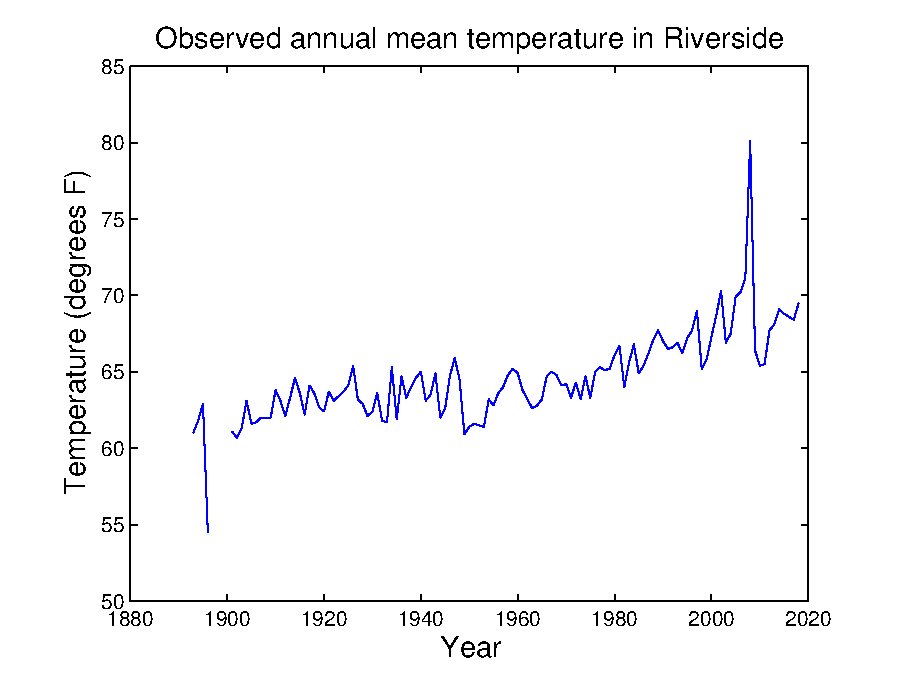
\includegraphics[width=\linewidth]{ch1-plot-temperature4.eps}
\caption{Observed annual mean surface temperature in Riverside.}
\label{fig:ch1-plot-temperature4}
\end{marginfigure}

Recall that the original global temperature data was given as an anomaly compared to the average over some baseline (or reference) period -- in this case, year 1910 to 2000. If we treated both data sets the same, and transformed the Riverside temperature data into a comparable anomaly, direct comparison could be made. To create an anomaly of the Riverside temperature data, relative to the mean of the data for years 1910 to 2000, requires the mean of the years 1910 to 2000 ... this is not difficult to do, but it better left for another time ... For now, take it as having a value of 64.2\degree F. So to create an anomaly for the Riverside temperature data, simply subtract 64.2 from the values in the annual mean data column (the 14th column, which you can also specify with \texttt{end}).

Finally, go back to the original global mean anomaly values (re-load the data set if necessary) and convert from the anomaly in \degree C to \degree F (i.e. simply multiply by \(1.8\) -- no offset (32\degree F) is required in this particular case). If you additionally, chose and set a sensible common y-axis scale for both plots, you might end up with a pair of graphs looking like Figures \ref{fig:ch1-plot-temperature5} and \ref{fig:ch1-plot-temperature6}.
\sidenote[][-2.5in]{There are all sorts of likely reasons for the differences. Firstly, the global mean surface temperature rise includes both ocean surface and land surface. Because of the higher heat capacity of the ocean, the ocean surface warms slower than the land, and the ocean accounts for ca. 70\% of the total global surface area. So it is somewhat inevitable that the warming trend will be stronger in Riverside. It may also be that the Riverside data is influenced by the 'urban heat island' effect, in which long0-term measured trends can be affected by increasing urbanization of the area surrounding the weather station. It may also be that the latitude and specific location of Riverside, sees much more warming that the global mean.}

\vspace{1mm}
\noindent\rule{4cm}{0.5pt}
\vspace{2mm}

\begin{marginfigure}[0.0in]
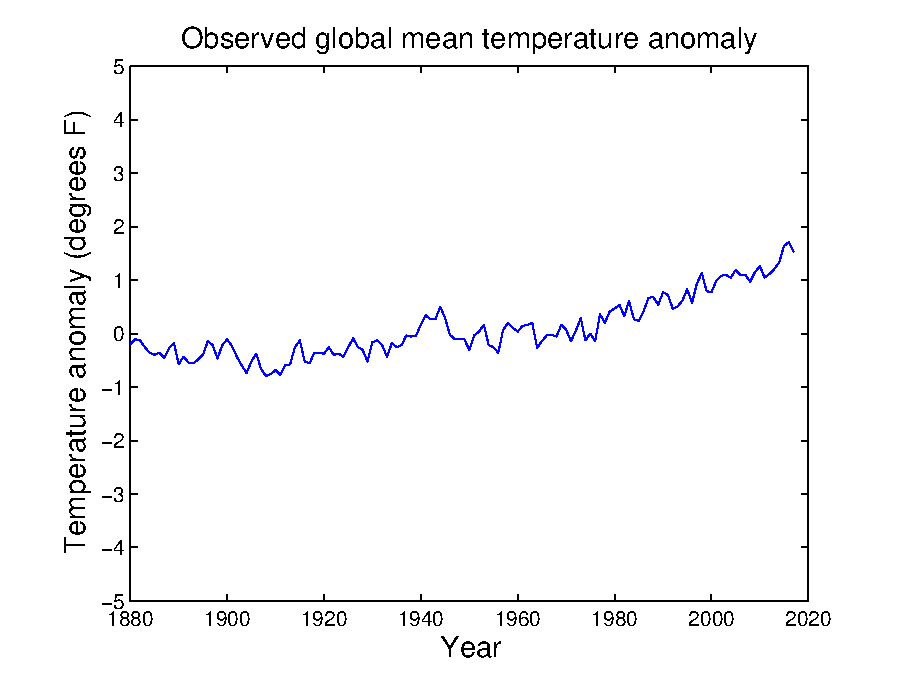
\includegraphics[width=\linewidth]{ch1-plot-temperature5.eps}
\caption{Observed global annual mean surface temperature anomaly, relative to the mean of 1910 through 2000.}
\label{fig:ch1-plot-temperature5}
\end{marginfigure}

\noindent Finally to some data filtering (row deletion) -- it was mentioned earlier that there were potential 'artifacts' in the Riverside mean annual temperature data. If you view the loaded in data array in the \textsf{Variable viewing window} (double-click on the \textsf{temperature\_riverside} variable name in the \textsf{Workspace window}), you can see for a number of years and months, rather than numbers, '\texttt{NaN}'s in the cells. \texttt{NaN} stands for 'Not a Number' and indicates that there is no (valid) numerical value for that array position (cell). The impact of there being a number of months of data missing, is that the annual mean is no longer a true annual mean but rather simply the mean of whatever monthly data exists for any particular year. For example, year 2008 has no data other than during the summer and the annual mean is hence simply equal to the July temperatures!

\begin{marginfigure}[0.0in]
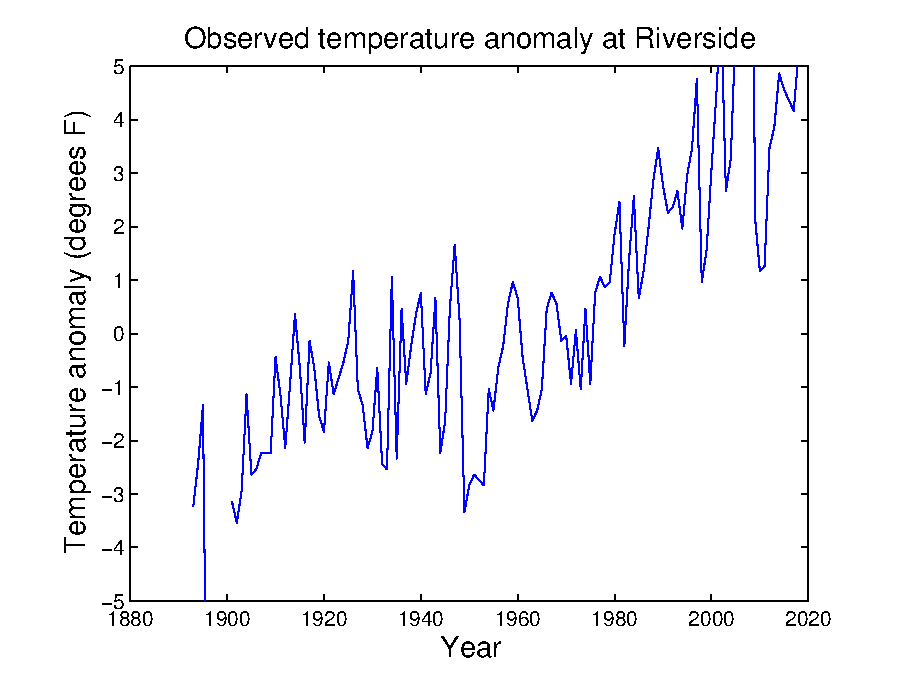
\includegraphics[width=\linewidth]{ch1-plot-temperature6.eps}
\caption{Observed annual mean surface temperature anomaly, relative to the mean of 1910 through 2000, at Riverside.}
\label{fig:ch1-plot-temperature6}
\end{marginfigure}

\begin{marginfigure}[0.0in]
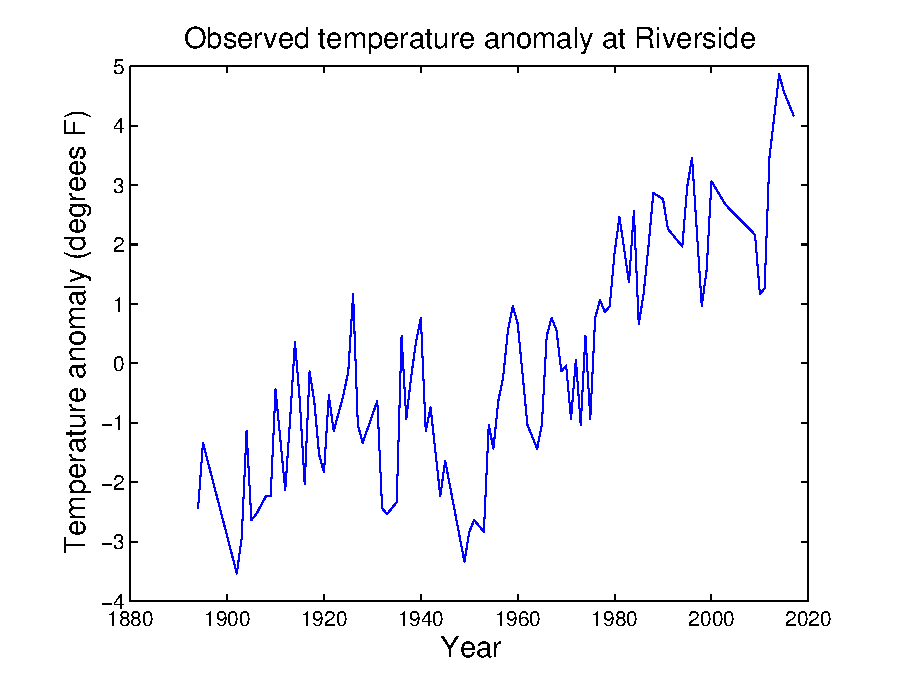
\includegraphics[width=\linewidth]{ch1-plot-temperature7.eps}
\caption{Observed annual mean surface temperature anomaly, relative to the mean of 1910 through 2000, at Riverside, filtered to remove years with missing monthly data.}
\label{fig:ch1-plot-temperature7}
\end{marginfigure}

One could address this by removing the years with (substantially) incomplete monthly data from the data file\sidenote{i.e. simply deleting the line in the file.} and prior to loading into \textbf{MATLAB}. Or would could process the data once in \textbf{MATLAB}. This can be done by assigning to particular row (vector) of data, an empty vector (\texttt{[]}). 

Taking first a simple example of a column vector:

\vspace{2mm}
\(A=\begin{pmatrix}1 \\
2 \\
3 \\
\end{pmatrix}\)
\vspace{2mm}

\noindent from which we wish to remove the 2nd row. In \textbf{MATLAB} we would create the vector by:

\begin{docspec}
>> A = [1; 2; 3];
\end{docspec}

\noindent and then remove the 2nd row by setting it to an empty element:

\begin{docspec}
>> A(2) = [];
\end{docspec}

Similarly, to remove the 2nd row of:

\vspace{2mm}
\(B=\begin{pmatrix}1 & 4 \\
2 & 5 \\
3 & 6 \\
\end{pmatrix}\)
\vspace{2mm}

\begin{docspec}
>> B = [1, 4; 2, 5; 3, 6];\\
>> B(2,:) = [];
\end{docspec}

\noindent (instead removing e.g. the 1st column would be \texttt{B(:,1) = []})

So back to the temperature data -- to for example remove the row containing the year 2008 data\sidenote[][-0.0in]{You can also delete rows (and columns) if you open up the \textbf{MATLAB} \texttt{Array window} (double-click on the variable name in the \texttt{Workspace window}). And ... edit/replace values ...}, which is row 11, we write:

\begin{docspec}
>> temperature\_riverside(11,:)=[];
\end{docspec}

Play this 'game' -- deleting as many row as you think result in biased means (because of missing monthly data)\sidenote[][-0.0in]{(being aware that as you delete rows, the numbering of the subsequent rows changes as the array size shrinks ...)}, with the Riverside temperature data, and re-plot the results.
For example, the result of removing ALL the rows with missing monthly data\sidenote{(There are simple and quick ways of doing this in \textbf{MATLAB} that we will see later.)}, results in Figure \ref{fig:ch1-plot-temperature7}.

%------------------------------------------------

\newpage

%------------------------------------------------

\section{Nicer graphing}

This section covers how to create slightly fancier plots in \textbf{MATLAB} and combines this with some more data loading practice.

%------------------------------------------------

\subsection{Modifying lines/symbols in \texttt{plot}}

The first deviant activity you can engage in with \texttt{plot}, is to graph the data without the line joining the points. Scrolling a little the way down \texttt{>> help plot}, it turns out that there are a number of options for color, line style, and marker symbol that you list together as a single parameter, straight after the parameters for \textit{x} and \textit{y} vectors. By default, \textbf{MATLAB} plots a solid line in blue with no marker points. Obviously, we could forego the sorting and plot a sane graphic (hopefully) by plotting just points and having no line between them. Hell, you could even be radical and use a different color ... Or, you could specify a symbol and no line.  The choice of colors is your oyster, as they (almost don't) say. e.g. Figure \ref{fig:plot-CO2basic3}. A summary of a few of the more common plotting options is provided in the Box. 

\marginnote[-2.25in]{\begin{mdframed}[backgroundcolor=light-gray, roundcorner=10pt,leftmargin=1, rightmargin=1, innerleftmargin=5, innerrightmargin=5, innertopmargin=5,innerbottommargin=5, outerlinewidth=1, linecolor=light-gray]
The main (i.e. not an exhaustive list) data display options for the \texttt{plot} function are:
\\(1) point style
\\\noindent \texttt{.} -- point, \texttt{o} -- circle, \texttt{x} -- x-mark, \texttt{+} -- plus, \texttt{*} -- star, \texttt{s} -- square, \texttt{d} -- diamond, \texttt{v} -- triangle (down).
\\(2) line style
\\\noindent \texttt{-} -- solid, \texttt{:} -- dotted, \texttt{--} -- dashed, and when specifying a point style, not specifying a line style results in no line.
\\(3) color 
\\\noindent  \texttt{b} -- blue, \texttt{g} -- green, \texttt{r} -- red,  \texttt{y} -- yellow, \texttt{k} -- black, \texttt{w} -- white.
\\To use them, add a new parameter when you call the \docenv{plot} \textit{function} -- whereas before, you typed, for plotting a vector y against x:
\begin{docspecmargin}
plot(x,y);
\end{docspecmargin}
now add, following a comma, the point and line style option, encased in a pair of inverted commas, e.g. for a red, dashed line:
\begin{docspecmargin}
plot(x,y,'r--');
\end{docspecmargin}
and for blue circles (no line):
\begin{docspecmargin}
plot(x,y,'bo');
\end{docspecmargin}
\end{mdframed}}

\begin{marginfigure}[-0.0in]
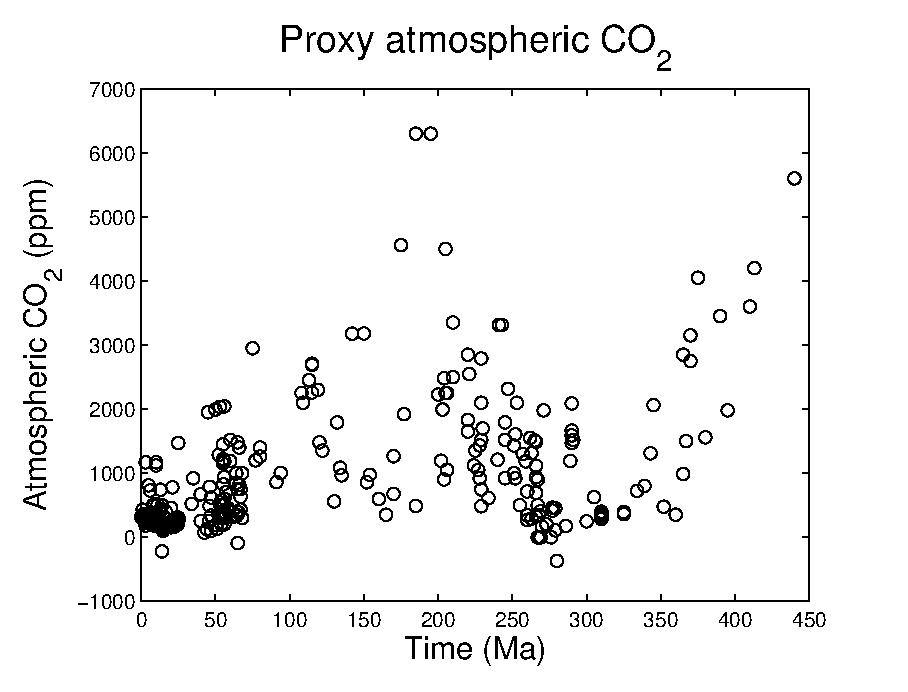
\includegraphics[width=\linewidth]{plot-CO2basic3.eps}
\caption{Proxy reconstructed past variability in atmospheric CO2 (sorted data).}
\label{fig:plot-CO2basic3}
\end{marginfigure}

%------------------------------------------------

\subsection{Plotting multiple data-sets}

So far, so good. But so boring, although simple marker-only and joined-by-line plots have their place. For a start, the original data-set included an estimate of the uncertainty in the CO\(_{2}\) reconstructions in the form of the min and max plausible value for each 'central' (best guess?) estimate. \textbf{Excel} can make plots incorporating errors, including non-symmetric errors, relatively easily. What about in \textbf{MATLAB}? (There is a function for this -- 
\docenv{errorbar}.), I have absolutely no idea. (This would make such a good exercise for the reader, as they (do) say.)

Personally, I might have been tempted to draw vertical bars alongside the data (most likely). Or plot with different symbols, with the min and max values as points. Or plotted min and max lines as a bounding envelope (lines). All of these require sone further little trick in \textbf{MATLAB}, which involves the command \docenv{hold}. This is nice and simple and takes the additional (2nd) word: \texttt{on}, or \texttt{off}.
\\ \texttt{>> hold on} -- will enable you to add additional elements to a graphic,
\\ \texttt{>> hold off} -- returns to the default in which a new graphic replaces the current on in a Figure window. 

\vspace{1mm}
\noindent\rule{4cm}{0.5pt}

\newpage

\marginnote[-0.0in]{\begin{mdframed}[backgroundcolor=light-gray, roundcorner=10pt,leftmargin=1, rightmargin=1, innerleftmargin=5, innerrightmargin=5, innertopmargin=5,innerbottommargin=5, outerlinewidth=1, linecolor=light-gray]
\docenvdef{errorbar}
\\Works like \texttt{plot}, except it adds error bars. The 2 most useful usages are:
\\\texttt{errorbar(x,y,err)} plots y versus x and draws a vertical error bar at each data point. All of \texttt{x}, \texttt{y}, and \texttt{err}, are vectors (all of the same length).
\\\texttt{errorbar(x,y,neg,pos)}draws a vertical error bar at each data point, where neg determines the length below the data point and pos determines the length above the data point, respectivel. All of \texttt{x}, \texttt{y}, \texttt{neg}, and \texttt{pos}, are vectors (all of the same length).
\end{mdframed}}

\marginnote[-0.0in]{\begin{mdframed}[backgroundcolor=light-gray, roundcorner=10pt,leftmargin=1, rightmargin=1, innerleftmargin=5, innerrightmargin=5, innertopmargin=5,innerbottommargin=5, outerlinewidth=1, linecolor=light-gray]
\docenvdef{hold}
\\According to \textbf{MATLAB} \textsf{help}:
\\\texttt{hold on} -- retains plots in the current axes so that new plots added to the axes do not delete existing plots.
\\\texttt{hold off} sets the hold state to off so that new plots added to the axes clear existing plots and reset all axes properties.
\end{mdframed}}

\newthought{As an example} -- set:

\begin{docspec}
>> hold on
\end{docspec}

\noindent and then plot the minimum and maximum CO\(_{2}\) values (columns \#3 and \#4) in different symbols and different colors, on top of your existing plot. If you want to then label what the different lines or sets of points are, you can add a legend with the \docenvdef{legend} command. For instance, if you have managed to successfully plot the mean CO\(_{2}\) values as discrete black circles, and the minimum and maximum uncertainty limits as blue and red lines, respectively, you could type:
\begin{docspec}
>> legend('Mean CO\_2','Lower uncertainty limit','Upper uncertainty limit');
\end{docspec}
(all one line) and it should end up looking like Figure \ref{fig:plot-CO2basic4}.

\begin{marginfigure}[0.5in]
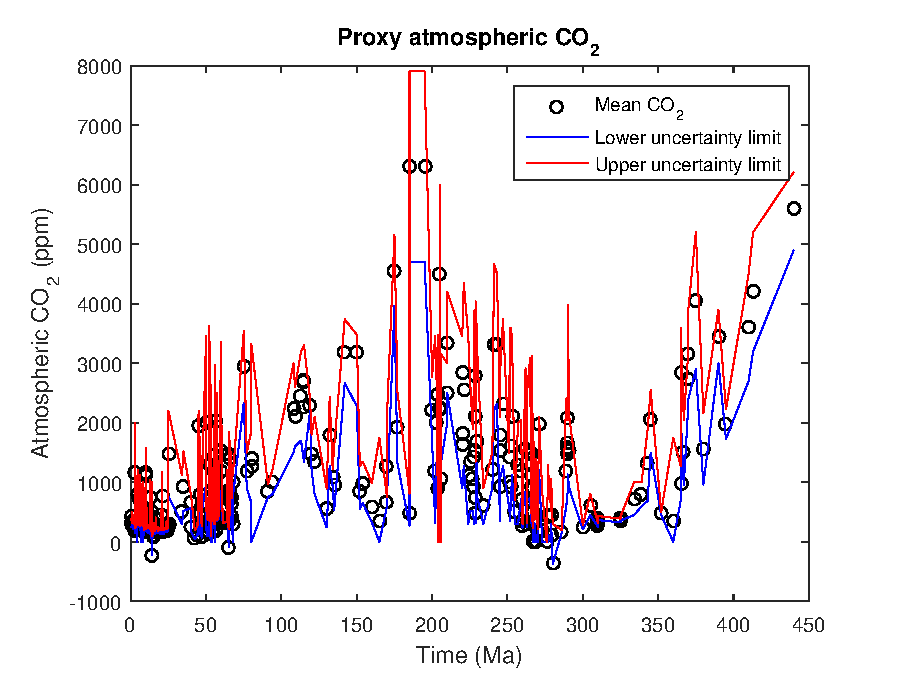
\includegraphics[width=\linewidth]{plot-CO2basic4.eps}
\caption{Proxy reconstructed past variability in atmospheric CO2 (sorted data).}
\label{fig:plot-CO2basic4}
\end{marginfigure}

\vspace{1mm}
\noindent\rule{4cm}{0.5pt}
\vspace{2mm}

\noindent Returning to the previous plotting Example, of the observed historical trend in global mean temperature vs. the temperature recorded in Riverside -- you now know how to plot BOTH temperature anomaly trends in the same \textsf{figure window} (and the same panel), so try it!

%------------------------------------------------

\subsection{Changing label font size (and type)}

The axis and title labels, by default, can be difficult to read when the graphics are saved and then imported into a document/paper. You can change the size of text as you create axis captions and figure titles etc., by specifying the value of an additional (text size) parameter in the function. For example, to increase the size of the x-axis label to a 14pt font:

\begin{docspec}
>> xlabel('Year','FontSize',14);
\end{docspec}

Here -- after the you have passed the string you wish to appear to the \textbf{MATLAB} \texttt{xlabel} \textit{function} (\texttt{'Year'}), there is a pair of additional parameters:

\begin{docspec}
'FontSize',14
\end{docspec}

The first additional parameter specifies the aspect of the axis label that you wish to change (here: \texttt{'FontSize'}), and the 2nd parameter of the pair, is the (new) value (here: \texttt{14}).\sidenote{See help on \texttt{xlabel}.} Similarly, the y-axis label and title text size can be adjusted in exactly the same way.

Other property parameters\sidenote{Again -- refer to \textbf{MATLAB} \textsf{help}.} that might be useful (to change), are (with example changes):

\begin{docspec}
'FontName','Courier'\\
'FontWeight','bold'\\
'FontAngle','italic'
\end{docspec}

%------------------------------------------------

\subsection{Scatter plots}

Returning back to the Phanerozoic proxy (CO\(_{2}\)) data, we can now put a different (graphical) spin on it.

\begin{marginfigure}[0.25in]
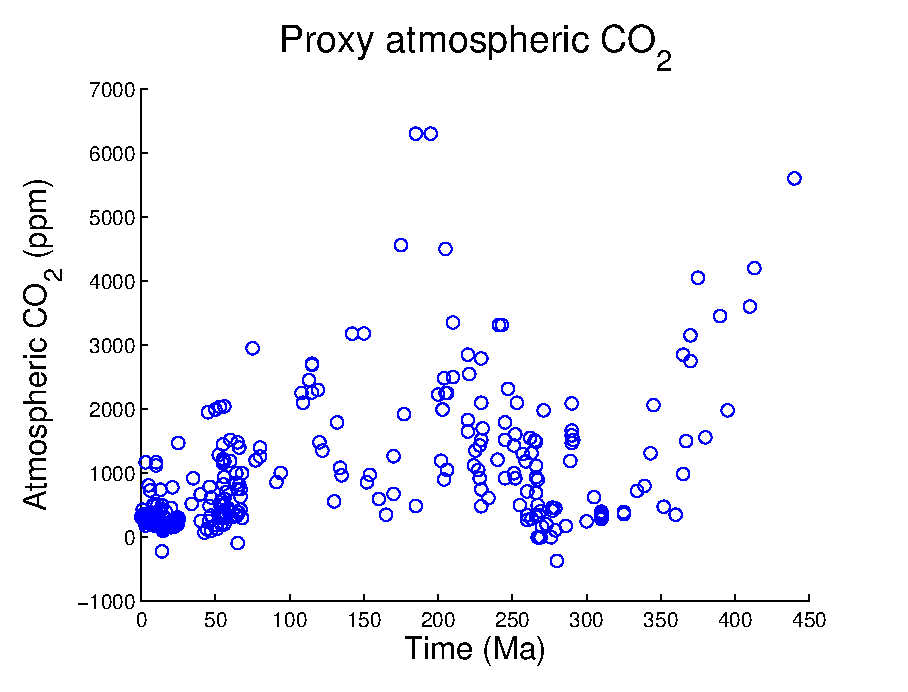
\includegraphics[width=\linewidth]{plot-CO2scatter.eps}
\caption{Proxy reconstructed past variability in atmospheric CO2 (scatter plot).}
\label{fig:plot-CO2scatter}
\end{marginfigure} 

Consider ... \docenvdef{scatter}. In fact, don't just considered it, \texttt{help} on it (\texttt{\textgreater\textgreater\ help scatter}). The simplest possible usage is, apparently:
\begin{docspec}
SCATTER(X,Y) draws the markers in the default size and color.
\end{docspec}
(where \texttt{X} and \texttt{Y} are vectors). This almost could not be more straight-forward.  Make yourself an \texttt{X} and \texttt{Y} vector out of the loaded-in dataset (or if you are feeling brave, you can pass in directly the appropriate parts of the dataset array), close the existing Figure window\sidenote[][-0.0in]{See earlier.}, and \texttt{scatter}-plot the (mean) CO\(_{2}\) data.

\begin{marginfigure}[-0.0in]
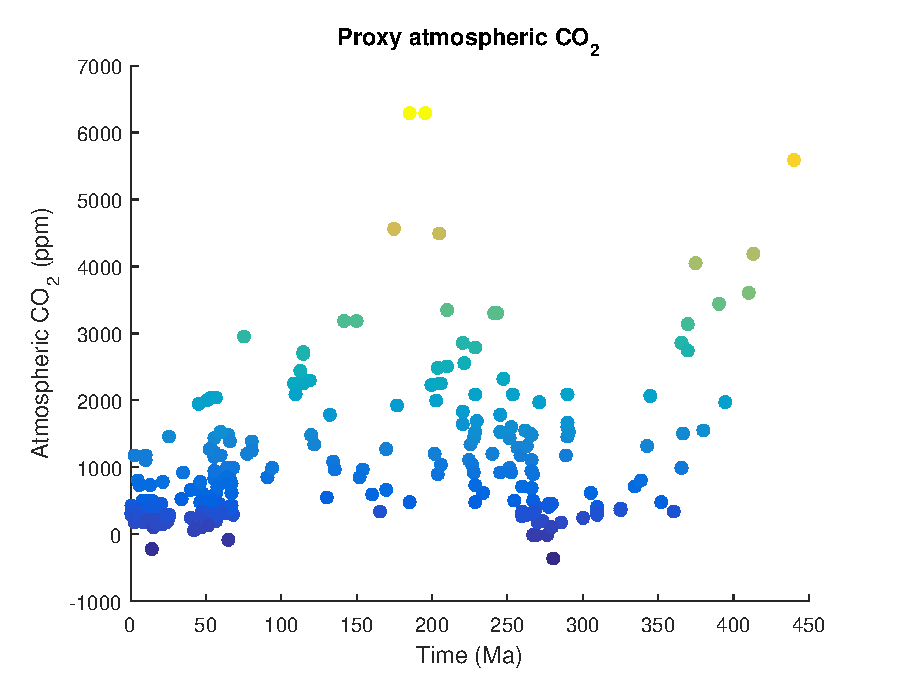
\includegraphics[width=\linewidth]{plot-CO2scatter2.eps}
\caption{Proxy reconstructed past variability in atmospheric CO2 (scatter plot).}
\label{fig:plot-CO2scatter2}
\end{marginfigure} 

Perhaps a little disappointingly, the default (Figure  \ref{fig:plot-CO2scatter}) (plus added labels) looks a little like one of the plots before. However, \texttt{scatter} can plot color-filled symbols, but more powerfully, can scale the fill color to a 3rd data value (vector), in a sort of pseudo 3D \textit{x}-\textit{y}-\textit{z} plot.  For instance, it will be duplicating information that is already presented (\textit{y}-axis), but you could color-code the points, by the y-value, i.e. the atmospheric CO\(_{2}\) value. e.g.
\begin{docspec}
SCATTER(data(:,1),data(:,2),20,data(:,2))
\end{docspec}
draws the markers with an (area) size of 20 (points), in different colors. Coloring just the outlines of the circles is perhaps not ideal (difficult to see all of the color differences), so the circles can be filled in instead (and you could make them a little larger too):
\begin{docspec}
SCATTER(data(:,1),data(:,2),40,data(:,2),'filled')
\end{docspec}
resulting in Figure \ref{fig:plot-CO2scatter2}.

\vspace{1mm}
\noindent\rule{4cm}{0.5pt}

%------------------------------------------------

\subsection{Simple 2D data and bitmap visualization}

There are 2 different simple \textbf{MATLAB} commands for visualizing a 2D dataset (i.e. a matrix) as a bitmap image (and via a 3rd command, viewing various bitmap photo and image format files too).

As something (2D data) to play with -- \texttt{load} in the data matrix: \texttt{model\_grid.txt}. Then, view the data in the array viewer, just to get a feel for what you are dealing with here (although you are unlikely to be much wiser after doing so). Lastly,  go ahead and employ the \docenv{pcolor} function in its simplest possible usage (see Box) to visualize the data. You can see (Figure \ref{fig:ch1-plot-pcolor1} ) that it is ... something. Maybe a little like the continents, but up-side-down at the very least. What to do?

\begin{marginfigure}[-2.0in]
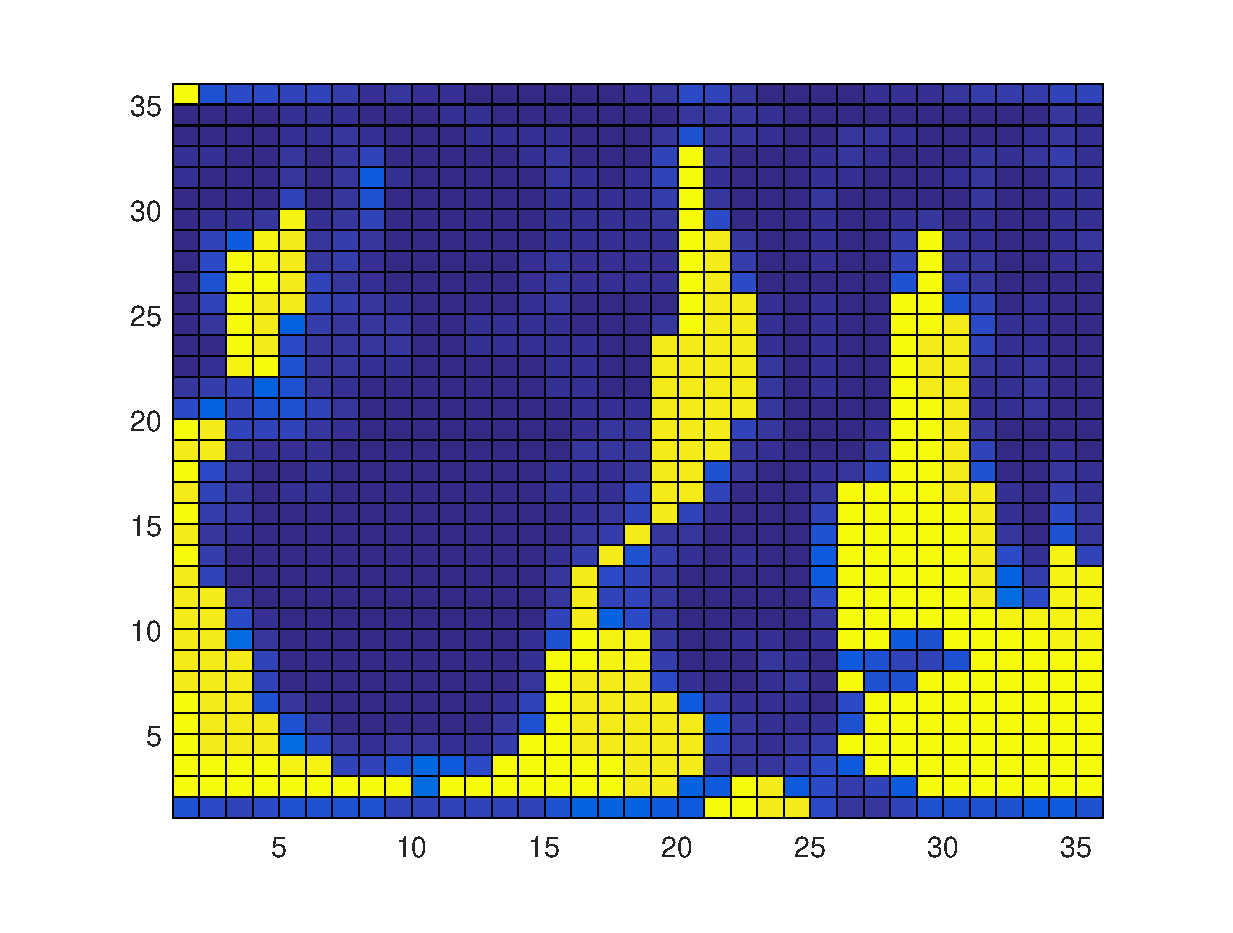
\includegraphics[width=\linewidth]{ch1-plot-pcolor1.eps}
\caption{A 2D plot of some random gridded model data.}
\label{fig:ch1-plot-pcolor1}
\end{marginfigure}

Well, it is a good job that you remember how to re-orientate arrays, right?\sidenote[][0.0in]{You don't? See earlier in the Chapter ...} If you guess right first time (three different basic transformations of a matrix were described), you will get Figure \ref{fig:ch1-plot-pcolor2}.

\begin{marginfigure}[0.75in]
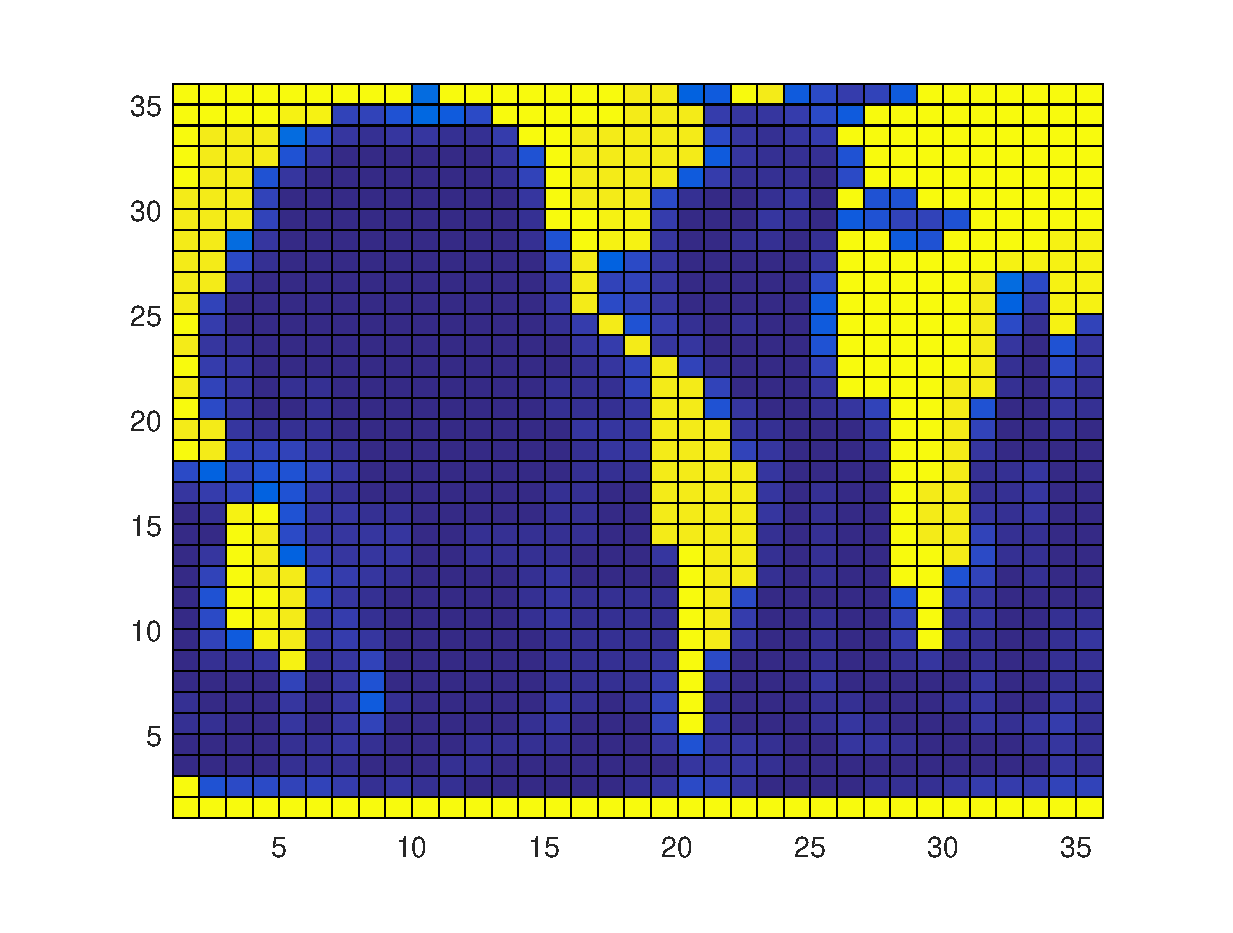
\includegraphics[width=\linewidth]{ch1-plot-pcolor2.eps}
\caption{A 2D plot of some random gridded model data ... but with the underlying data matrix re-orientated before plotting.}
\label{fig:ch1-plot-pcolor2}
\end{marginfigure}

Next try something very similar. but using the \docenv{image} function.\footnote{Now the model grid is the correct way around! I have absolutely no idea why and why it is reading the matrix dimensions differently from \docenv{pcolor}. I am sure you could \textbf{Google} and find out. But you would have to actually care first.} 

\marginnote[0.0in]{\begin{mdframed}[backgroundcolor=light-gray, roundcorner=10pt,leftmargin=1, rightmargin=1, innerleftmargin=5, innerrightmargin=5, innertopmargin=5,innerbottommargin=5, outerlinewidth=1, linecolor=light-gray]
\docenvdef{pcolor}
\\MATLAB claims that pcolor(C) plots; "a rectangular array of cells with colors determined by C. Actually, I believe \textbf{MATLAB} on this.
So if you have a matrix, \textbf{MATLAB} will plot a regular arrays of cells, with each cell representing one of the elements in the matrix, and will color that cell according to the value. (\texttt{pcolor} will by default, autoscale how the color scale maps onto the data in the matrix such that both extreme ends of the color scale are used.)
\end{mdframed}}

\marginnote[-0.25in]{\begin{mdframed}[backgroundcolor=light-gray, roundcorner=10pt,leftmargin=1, rightmargin=1, innerleftmargin=5, innerrightmargin=5, innertopmargin=5,innerbottommargin=5, outerlinewidth=1, linecolor=light-gray]
\docenvdef{image}
\\You can import an image, such as in \texttt{.jpg}, \texttt{.tiff}, or \texttt{.png} format, using \docenvdef{imread} -- simply pass it the name of an image file (as a string, this variable name needs to be encased in inverted commas) and assign the results to a variable name of your choice. Then plot (using \texttt{image}) that variable.
\end{mdframed}}

What is the point of this? You now have the ability to simply visualise a gridded dataset. Later, we'll be doing it more formally  and it gets rather more involved when you have to create matrixes to describe the grid dimensions (e.g. lon and lat) for yourself.

As your very last exercise -- find an image on the internet that amuses you, download it, load it into \textbf{MATLAB} (using \docenv{imread}), visualize it using \texttt{image}, and then ... well, that depends on how amusing it is. Maybe try plotting something on top of it (using \texttt{hold on}) or simply go home.

%------------------------------------------------

\newpage

%------------------------------------------------

\section{Further matrix math (systems of equations)}

%------------------------------------------------
%
You can also use \textbf{MATLAB}'s powerful matrix functionality to solve real-world problems for you.

\newthought{As an example} -- consider the Great Lakes -- the largest lake system in the world. They have on their shores some of the greatest cities ... as well as some of North Americas worst hockey teams. More importantly, much of the region is heavily industrialised and there is hence an exciting potential for pollution input into the lakes and hence a contrived numerical modelling exercise.

The layout of the lake system is shown schematically in Figure \ref{fig:ch4-lakes_schematic}, together with the mean volumes of the lakes and the annual flow rate of water out of them.

A cocktail of heavy metals pours into each lake, the amount dependent largely upon the population within the catchments of the lake. The input rates to each of the 5 lakes are given below.

\begin{table}[h]\index{typefaces!sizes}
\footnotesize%
\begin{center}
\begin{tabular}{lccl}
\toprule
\ Lake & Heavy Metal Input (kg yr\(^{-1}\)) \\
\midrule
\ Superior & 1.0\(\times\)10\(^{3}\) \\
\ Michigan & 4.5\(\times\)10\(^{3}\) \\
\ Huron & 1.0\(\times\)10\(^{3}\) \\
\ Erie & 3.5\(\times\)10\(^{3}\) \\
\ Ontario & 3.0\(\times\)10\(^{3}\) \\
\bottomrule
\end{tabular}
\end{center}
\caption{Pollution input input rates to each of the 5 lakes.}
\label{tab:ch4-laketable}
\end{table}

The steady state concentration of heavy metals in the Great Lake system (the steady state solution being the state in which none of the concentrations in any of the lakes is changing) is something that you can find an analytical solution for. You have 5 unknowns (the concentration in each of the 5 lakes) and you can write down a series of 5 equations involving these unknowns. (There is slightly more to it than this, as there must also exist an inverse for the matrix, which is not always the case ...)

\begin{marginfigure}[0.0in]
\includegraphics[width=\linewidth]{ch4-lakes_schematic.tif}
\caption{Lake volumes and river flow rates in the Great Lakes system.}
\label{fig:ch4-lakes_schematic}
\end{marginfigure}

Lets call the concentrations (kg km\(^{-3}\)) of heavy metals in the lakes; \texttt{cS}, \texttt{cM}, \texttt{cH}, \texttt{cE}, and \texttt{cO} (for; Superior, Michigan, Huron, Erie, and Ontarion, respectively). At steady-state, the inputs of heavy metals must exactly balance the outputs from each lake (otherwise, the concentration in the lake would change and the system would not be at steady-state). We can write a series of mass-balance equations for the 5 lakes. For instance, in Lake Superior, the metal input flux is 1.0\(\times\)10\(^{3}\) kg yr\(^{-1}\) (1000 kg yr\(^{-1}\)). This must balance the loss of metals in the river outflow if the concentration of metals in the lake is to remain constant. The water outflow rate that is given to you is 63 km\(^{3}\) yr\(^{-1}\). The metal outflow flux is then just the concentration of metals in the water (\texttt{cS}), times by the water flow; \texttt{63*cS}. Thus, for Lake Superior, we can write \texttt{1000 = 63*cS}. The other lakes can be similarly analysed, to give a set of 5 equations:

\begin{docspec}
1000 = 63*cS 
\\4500 = 47*cM
\\1000 + 63*cS + 47*cM = 157*cH
\\3500 + 157*cH = 173*cE
\\3000 + 173*cE = 208*cO
\end{docspec}

It is not hard to work your way down these, solving first (\texttt{cS = 1000/63} is not so hard to solve ...) and then the 2nd, which then allows you to solve the 3rd, before then solving the 4th and 5th in turn .... However, the system of equations you might have to solve could be (and usually is) much more complicated. Fortunately, we can get MATLAB to do the work. :) It may be far from obvious what \textbf{MATLAB} has to do with this, so I'll do a little re-arranging of the 5 equations:

\begin{docspec}
\ 63*cS + \ \ 0*cM + \ \ 0*cH + \ \ 0*cE +  \ \ 0*cO = 1000
\\\ \ 0*cS + \ 47*cM + \ \  0*cH + \ \ 0*cE +  \ \ 0*cO = 4500
\\ -63*cS + -47*cM + 157*cH + \ \ 0*cE +  \ \ 0*cO = 1000 
\\\ \ 0*cS + \ \ 0*cM - 157*cH + 173*cE +  \ \ 0*cO = 3500
\\\ \ 0*cS + \ \ 0*cM + \ \ 0*cH - 173*cE + 208*cO = 3000 
\end{docspec}

This is starting to look scarily like some matrix stuff. Satisfy yourselves that these two sets of equations  are the same, and that all I have done is to write them with the unknowns on the left hand side (\texttt{cS}, \texttt{cM}, \texttt{cH}, \texttt{cE}, and \texttt{cO}) and the knowns (the metal input fluxes) on the right hand side. In fact, this can be written in matrix form:

\begin{docspec}
\(\begin{pmatrix}
63 & 0 & 0 & 0 & 0 \\
0 & 47 & 0 & 0 & 0 \\
-63 & -47 & 157 & 0 & 0 \\
0 & 0 & -157 & 173 & 0 \\
0 & 0 & 0 & -173 & 208 \\
\end{pmatrix}
\times
\begin{pmatrix}
cS \\
cM \\
cH \\
cE \\
cO \\
\end{pmatrix}
=
\begin{pmatrix}
1000 \\
4500 \\
1000 \\
3500 \\
3000 \\
\end{pmatrix}\)
\end{docspec}

Brush up on your matrix maths and check that Eq. 5 is exactly the same as before. It is just the series of 5 separate equations, but represented in matrix math form. Write out the matrix multiplication in full to get the 5 separate equations back again if you are not convinced that this is the case.

In a new \textbf{MATLAB} \textsf{m-file}, create a 5\(\times\)5 array containing the values in the matrix on the left hand side of the equation above and assign it to the variable \texttt{R} (for \uline{R}iver flow). Create a 5\(\times\)1 array containing the vector values on the right hand side of the equation and assign it to the variable \texttt{F} (for heavy metal \uline{F}lux). The solution to this problem is the set of (steady-state) concentrations of heavy metals in the 5 lakes. (Call this variable \texttt{C}.) We thus have the equation:
\begin{docspec}
\(R \times C = F\)
\end{docspec}

If we could determine the inverse of \texttt{R}, we could write:
\begin{docspec}
\(R^{-1} \times R \times C = R^{-1} \times F\)
\end{docspec}
\noindent (I have simply multiplied both sides of the equation by \texttt{R\(^{-1}\)}.)

Recognizing that a matrix (\texttt{R}) multiplied by its inverse (\texttt{R\(^{-1}\)}) is the Identity matrix (\texttt{I}), and that \texttt{I} leaves everything it multiplies alone, we have:
\begin{docspec}
\(I \times C = R^{-1} \times F\)
\\\(\Rightarrow C = R^{-1} \times F\)
\end{docspec}

We are there! We have R and F, so by multiplying \texttt{F} by the inverse of R, we get our set of 5 solutions (in the 5\(\times\)1 vector \texttt{C}). And \textbf{MATLAB} will give you the inverse of \texttt{R} (if it exists) on a plate.\sidenote{At the command line; type:
\begin{docspecmargin}
>> help inv
\end{docspecmargin}
to find out how to get your paws on the inverse of \texttt{R}. You can also lookup 'inverse of a matrix' in the Index of \textbf{MATLAB} Help.} Sweet deal!

Now you have everything you need -- go solve the steady-state problem for the unknown metal concentrations in the 5 lakes (the vector array \texttt{C}) using the inverse of \texttt{R}. You can always plug these values into the original equations  to satisfy yourselves that it all works out.\sidenote{Note that the equations above are written in normal maths language, e.g. with a \(\times\) rather than the \texttt{*} that \textbf{MATLAB} understands.}

%----------------------------------------------------------------------------------------
% CHAPTER 2
%----------------------------------------------------------------------------------------

\chapter{Elements of ... programming}
\label{ch:02}

%------------------------------------------------

\begin{fullwidth}

\newthought{Nerd.} This is what you are now going to become. And lose all your social skills. And sit at home all day in front of your computer. Which has become your only friend.

You will achieve this higher state of Being by starting to learn to write and use \textit{scripts} and \textit{functions} (aka \texttt{m-files}) in \textbf{MATLAB}. Actually, at this point you are now writing computer programs (of a sort) rather than endlessly typing stuff at the command line in the forlorn hope that something useful might occur.
You will also be doing a great deal of code debugging ...
\end{fullwidth}

%------------------------------------------------

\newpage

%------------------------------------------------

\section{Introduction to scripting (programming!) in MATLAB}

Commands in \textbf{MATLAB} can become very lengthy, and you typically end up with multiple lines of code to get anything even remotely useful done. And as you have noticed, it can take a lot of time to enter in all these lines. When when you log off and go home ... it is all gone. \sidenote[][-0.5in]{\textbf{MATLAB} remembers all the commands used in previous session (although this may not be the case of shared, lab computers) and lists them in the \textsf{Command History window}. You can recover and re-execute a previous command in this list by double-clicking it. You can also re-run more than one line at a time by selecting multiple lines and pressing \textsf{F9} (or \textsf{Evaluate Selection} from the (R-mouse button in \textbf{Windows}) context menu).} ... If only there was some way of storing all these commands in such a way that they could be worked on and run again with the press of a button (as a wild guess, how about \textsf{F5}?), without having to enter them all in, all over again from scratch ...

\marginnote{\begin{mdframed}[backgroundcolor=light-gray, roundcorner=10pt,leftmargin=1, rightmargin=1, innerleftmargin=5, innerrightmargin=5, innertopmargin=5,innerbottommargin=5, outerlinewidth=1, linecolor=light-gray]
\textit{\textbf{\textcolor[rgb]{0.501961,0,0}{m-file}}}
\\... is nothing more than a simple text file, in which a series of one or more \textbf{MATLAB} commands are written and which via the \textsf{.m} file extension, \textbf{MATLAB} interprets as a program file (\textit{script} or \textit{function}) that can be edited and executed (or rather, the list of commands inside, can be executed in sequential order).
\\Assume a similar convention to that for \textit{variables} in the naming of \textit{m-files}.
\end{mdframed}}

Your wish is granted! In \textbf{MATLAB}, it is possible to store all of your commands in a single text file, and then request that they (the list of commands) are all executed (sequentially)  at one go. \textbf{MATLAB} gives this text file a fancy name (because it is a very fancy piece of software, after all) -- a \textit{script}\sidenote{The conception of a \textit{function}, will be introduced later.}, otherwise known as an \textit{m-file}.  To create a new \textit{m-file}; from the  \textsf{File menu}, select \textsf{Script} (a common type of \textit{m-file})\sidenote[][0.0in]{In order version of \textbf{MATLAB}: \textsf{File}/\textsf{New} menu, and select: \textsf{Blank M-file}.}. You will see a text editor (more fancy-ness) appear in front of your very eyes, containing your requested (but currently empty) \textit{m-file}. Save the \textit{m-file} to your directory of choice. Alternatively, simply create a new (blank) text file and save it with the extension \textsf{.m}, rather than e.g. \textsf{.txt} -- this creates you a (script) \textit{m-file} (illustrating that an \textit{m-file} is nothing more than a text file with a \textsf{.m} file extension). From an \textit{m-file}, you can issue all the \textbf{MATLAB} commands you previously would have entered individually, line-by-tedious-line, at the command line. Furthermore, having created and saved  a \textbf{MATLAB} script, it can be executed again and as many times as you like.
 
You can execute an \textit{m-file} by typing its name into the \textsf{Command window} (omitting the \textsf{.m} file extension). Ensure that \textbf{MATLAB} is operating in the same directory as the directory that you have saved your \textit{m-file}. You can also run the \textit{script} (\textit{m-file}) by hitting the big bright green Run icon button at the top of the \textit{m-file} editor\sidenote[][-0.25in]{In older versions of \textbf{MATLAB} -- select: \textsf{Debug}/\textsf{Run} from the 'debug' menu of the \textsf{Editor window}.}. The short-cut for running it is to whack your paw down on the Function Key \textsf{F5}.

OK -- you are now ready for your very first program ... inevitably ... this has to be to print 'Hello World' to the screen. No, really. (\textbf{Google} it.) 

Create a new \textit{m-file}, calling it e.g. \textsf{hello\_world.m} (remembering that spaces are NOT allowed in filenames). You are going to use the function \docenv{disp} (see margin help box and/or type \texttt{>> help disp}  to find out the \textbf{MATLAB} \textit{function} syntax and usage). This command (/\textit{function})  will print to the screen, either any text you specify (in inverted commas), or the contents of any\textit{} \textit{variable} (you pass the variable name to \texttt{disp}). For now, simply pass the text directly.

\marginnote[-2.0in]{\begin{mdframed}[backgroundcolor=light-gray, roundcorner=10pt,leftmargin=1, rightmargin=1, innerleftmargin=5, innerrightmargin=5, innertopmargin=5,innerbottommargin=5, outerlinewidth=1, linecolor=light-gray]
\docenvdef{disp}
\\... displays something (the contents of a variable) to the screen.
\\In the example of:
\begin{docspecmargin}
disp(STRING)
\end{docspecmargin}
where \texttt{STRING} is a .... \textit{string}, you get the \textit{string} displayed as text at the command line.
\\You can also pass the name of any variable
\begin{docspecmargin}
disp(VARIABLE)
\end{docspecmargin}
and get the contents of \texttt{VARIABLE} displayed.
\\Note that the difference between using \docenv{disp} and simply typing the variable name:
\begin{docspecmargin}
disp(X)
\end{docspecmargin}
is ... well, find out for yourself!
\\Note that in some situations, its effect is simply the same as leaving off the semi-colon (\texttt{;}) from the end of a line.
\end{mdframed}}

Your program needs just a single line in the \textit{m-file}:
\begin{docspec}
disp('hello, world')
\end{docspec}
\noindent Save the file (to your working directory). Run it at the command line by typing its name (omitting the \textsf{.m} extension). Your first program is a success! (Surely you could not screw up a single line program ... ?\sidenote[][-0.375in]{If \textbf{MATLAB} gives you an error message something like \\\textcolor{red}{\texttt{Undefined function or variable 'hello\_world'}} \\\noindent then it is likely you are simply not in the same directory as the \textit{m-file}, and/or the location of the \textit{m-file} is not in one of the directory paths \textbf{MATLAB} knows about (see previous Tutorials for comments on changing directory vs. adding paths.).}) 

You could extend this to a mighty 2-line program by defining the string as a variable and displaying the contents of the variable, i.e.,
\begin{docspec}
message = 'hello, world';
\\disp(message)
\end{docspec}

\noindent (Try this out.)\sidenote[][0.25in]{Remember that when a \textit{function} requires a \textit{string} input, you can either pass the string directly (encased in inverted commas), or assigned the string to a variable, and pass the name of the variable (no inverted commas).}

For further practice -- pick one of any of the previous exercises in which multiple lines of code were required, such as loading and then plotting a data set, place these lines into a new \textit{m-file }(either by re-typing them in or copying them out of the \textsf{Command History window}), save the file (to the same directory that you are working from), and run it my typing its name at the command line (omitting the \textsf{.m} extension).


%------------------------------------------------

\subsection{Programming good practice}

A few tips about good practice in (\textbf{MATLAB}) programming before we go on (and on and on and on):

\marginnote[-0.5in]{\begin{mdframed}[backgroundcolor=light-gray, roundcorner=10pt,leftmargin=1, rightmargin=1, innerleftmargin=5, innerrightmargin=5, innertopmargin=5,innerbottommargin=5, outerlinewidth=1, linecolor=light-gray]
\textbf{Creating \texttt{help} text in an \texttt{m-file}}
\\\textbf{MATLAB} allows you to crete a 'help' section in the \textbf{m-file} -- text that is outputted too the screen if you type help on that particular \textit{script} (or \textit{function}). The text is defined by a block of comment lines at the very top of the script file (or after the function definition in the case of a function). The last sequential comment line is taken to be the end of the help section. Note that the help section can be a minimum of eon single line.
A typical basic format is:
\begin{enumerate}[noitemsep]
\item Name of (in capitals), and very brief summary, of the script (/function).
\item List and description of the different forms of use (if there are one or more optional parameters) including definition of the input parameters.
\item Examples.
\item A \texttt{See also} section listing similar or related scripts or functions.
\end{enumerate}
\end{mdframed}}

\begin{itemize}[noitemsep]
\setlength{\itemindent}{.2in}

\item Choose helpful \textit{variable} names so that it is clear what each \textit{variable} represents. Avoid *excessively* short names, except for simple index and counting \textit{variables}. At the other extreme -- excessively long names, which the might be wonderfully descriptive, can lead to even simple calculation stretching over multiple lines of code (which can make it more difficult to see what is going on in the code overall).

\item Use comments within your \textit{m-file} to add explanation and commentary on your program. Anything after a \texttt{\%} on the same line is a considered a comment\sidenote{Your \texttt{\% comment} can start on a new line, or follow on from the end of a line of code, whichever is more helpful.}, and is ignored by \textbf{MATLAB}.

\item Structure the code nicely. You can break the code up into sections, e.g. by adding a blank line. You might also start each section with a label summarizing that it is going to do (via the addition of a \textit{comment} line).

\item To start with -- program in as simple a step-by-step way as possible. Breaking a complex calculation into several lines of simpler calculations is much easier to debug and work out what you were doing later, particularly if comments are also added. For all practical purposes -- at this level, everything will run just as fast whether as a complex calculation on one line, or simple bite-sized calculation spread over 4 lines with comment sin between. 

\item Always save your changes before running your program (or you may unknowingly be running the previous version).

\item If using the \textit{script} to do some plotting, sometimes (but not always) it is convenient to add at the top of the \textit{m-file}, \begin{docspec}
close all;
\end{docspec}
This command close all currently open figures, plots, images, etc. so that if you repeatedly run the script such as you might in developing and debuggin it, you don't end up with 1000000000s of \textsf{Figure windows} open ...

\end{itemize}

\vspace{1mm}
\noindent\rule{4cm}{0.5pt}
\vspace{2mm}\

\noindent An illustration (and a far from perfect illustration) of a short \textit{function} (\textit{m-file}) exhibiting at least a few examples of good practice, is:

\begin{docspec}
\textcolor{blue}{function} [dum\_temp] = ebm\_basic(dum\_S0)
\textcolor[rgb]{0,0.501961,0}{\\\% 0D case of EBM -- analytical solution
\\\% function takes one parameter -- the solar constant (units of W m-2) [NB. modern value: 1370.0]
\\\% define constants}
\\const\_0C = 273.15; \textcolor[rgb]{0,0.501961,0}{\% (units: K)}
\\const\_sigma = 5.67E-8; \textcolor[rgb]{0,0.501961,0}{\% Stefan-Boltzmann constant (units: W m-2 K-1)}
\textcolor[rgb]{0,0.501961,0}{\\\% define model parameters}
\\par\_emiss = 0.62; \textcolor[rgb]{0,0.501961,0}{\% (non-dimensional)}
\\par\_albedo = 0.3; \textcolor[rgb]{0,0.501961,0}{\% mean albedo}
\textcolor[rgb]{0,0.501961,0}{\\\% solve for surface temperature
\\\% equilibrium equation:
\\\% (1.0-par\_albedo)*(par\_S0/4.0) = par\_emiss*const\_sigma*loc\_temp\(^{\wedge}\)4.0
\\\% then re-arranged to:}
\\loc\_temp = ...
\\( (1.0-par\_albedo)*(dum\_S0/4.0)/par\_emiss/const\_sigma )\(^{\wedge}\)0.25;
\textcolor[rgb]{0,0.501961,0}{\\\% convert temperature units (Kelvin to Celsius) and set value of return variable}
\\dum\_temp = loc\_temp - const\_0C;
\textcolor{blue}{\\end}
\end{docspec} 

\begin{marginfigure}[0.0in]
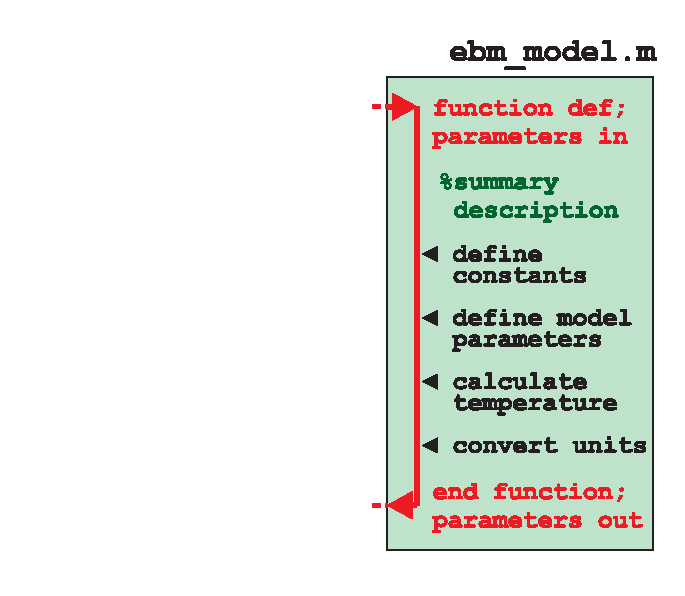
\includegraphics[width=\linewidth]{ch2-example.eps}
\caption{Schematic of the example program.}
\label{fig:ch2-example}
\end{marginfigure}

\noindent The schematic for the program structure is shown in \ref{fig:ch2-example}. (Don't worry what this particular program does, just note how I\ have structured it.)
 
This example also illustrates one possibility for a consistent \textit{variable} naming convention -- constants (\textit{variables} which never change in value) start with a \texttt{const\_} and parameters (variables whose values might be changed) with \texttt{par\_}, temporary ('local') variables with \texttt{loc\_} and variables passed into and out of the function: \texttt{dum\_}. Note the use of the semi-colon at the end of every line to prevent (here unwanted) printing of results to the screen. (Don't worry about what a \textit{function} is yet ... just not the degree of commenting and that there is some sort of consistent and meaningful naming convention.)

In the file, you can create as much 'ASCII art' as you like if it helps to make the code clearer, e.g. adding separator comment lines ...

\begin{docspec}
\textcolor[rgb]{0,0.501961,0}{\% ------------------------------------------------}
\end{docspec} 

... or highlighting certain section headers, e.g.

\begin{docspec}
\textcolor[rgb]{0,0.501961,0}{\% *** PLOTTING\ SECTION\ ***}
\end{docspec}

\noindent If it (a line) starts with a percentage symbol, then \textbf{MATLAB} ignores it and you can type whatever you like after it (on the same line).

\noindent Also note, if it helps -- you can run a single line of code over 2 lines of the file by adding

\begin{docspec}
...
\end{docspec}

\noindent at the end of a partial line (that is to be treated by \textbf{MATLAB} as joined continuously to the next line).

Your \textsf{Hello World} program might look like the following once it has had a little tune-up (although in this example this is pretty much over-kill):
\begin{docspec}
\textcolor[rgb]{0,0.501961,0}{\\\% program to print 'Hello World' to the screen
\\\% *** START ***
\\\% first -- define the text to display and assign it to the variable  message}
\\message = 'hello, world';
\textcolor[rgb]{0,0.501961,0}{\\\% second -- display the contents of variable message}
\\disp(message)
\textcolor[rgb]{0,0.501961,0}{\\\% ***\ END ***}
\end{docspec}

The book schematic structure of this program (\textit{script}) is shown in Figure \ref{fig:ch2-hello_world}.\sidenote{Note that not all of the comment lines are shown in the structure schematic -- only the main program summary at the top.}

\begin{marginfigure}[-0.0in]
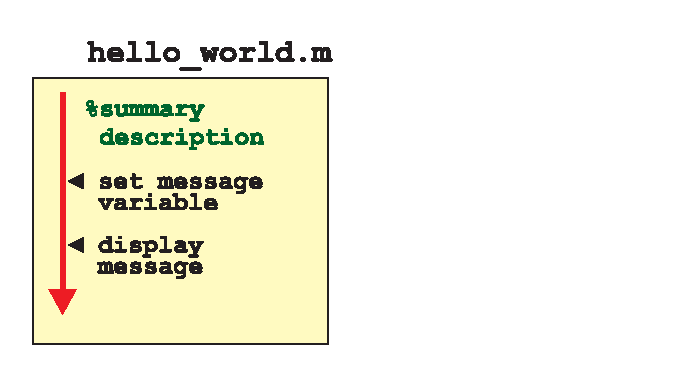
\includegraphics[width=\linewidth]{ch2-hello_world.eps}
\caption{Schematic of the Hello World program.}
\label{fig:ch2-hello_world}
\end{marginfigure}

Finally, and related to the next subsection -- code in stages, testing the (partial) code at each step. \uline{Do not} try and write all the code in one go and only try it out at the end\sidenote{Because it will not work 99 times out of 100 ...}.

%------------------------------------------------

\subsection{Debugging the bugs in buggy code}

What programming is mostly about is not writing new code so much as debugging\sidenote{The art of fault-finding in computer code.} what you have already written. Key then, is to reduce the incidence of bugs occurring in the first place, and when they do occur, firstly to have code that lends itself to debugging and secondly, knowing how to go about the debugging. The first two facets are at least partly addressed through good programming practice (see earlier)\sidenote{And by the discipline of software engineering, which is way out of scope of this course.}.

Here is an example to try out to start to see what might be involved in debugging,  loosely based on a previous plotting example -- go create a new \textit{m-file} called: \textsf{plot\_some\_dull\_stuff.m}\sidenote{Remember -- you are advised to name your \textit{m-files} as something vaguely descriptive of what the script actually does (and you do ont have to go with this choice, although it might turn out to be perfectly descriptive ;) (i.e. you do not have to call it this!)}. Then add the following lines to the file:

\begin{docspec}
\textcolor[rgb]{0,0.501961,0}{\% my dull plotting program
\\\% first, initialize variables and close existing figure windows}
\\close \textcolor[rgb]{0.501961,0,1}{all};
\\x = -2*pi:0.1:2*pi;
\\y1 = sin(x); 
\\y2 = cos[x];
\textcolor[rgb]{0,0.501961,0}{\\\% open a figure window and plot a sine graph}
\\figure;
\\plot(x,y1,\textcolor[rgb]{0.501961,0,1}{'r'});
\textcolor[rgb]{0,0.501961,0}{\\\% add a cosine graph} 
\\hold \textcolor[rgb]{0.501961,0,1}{on};
\\plot(x,y2,k);
\end{docspec} 

\noindent and then run it (refer to earlier for how).

Pretty dull stuff eh? Wait -- maybe you didn't get a figure appearing on the screen with a pair of sines and cosines on. Has \textbf{MATLAB} given you an error? If you typed in the above 'correctly', you should see:
\begin{docspec}
\textcolor{red}{Error: File: plot\_some\_dull\_stuff.m Line: 6 Column: 9
Unbalanced or unexpected parenthesis or bracket.}
\end{docspec}

\noindent Actually ... if this were your program, you should have paid attention to earlier and not have written it all at once before testing it! But at least \textbf{MATLAB} is giving you some sort of feedback. The actual error reported might not always mean that much to you but the line number at which the problem occurred is gold-dust. The line of code is does not like is line 6\sidenote{Note that although \textbf{MATLAB} ignores comment lines (in the context of executing code), it does count them when telling you which line of the program code an error occurs at.}, which is:

\begin{docspec}
y2 = cos[x];
\end{docspec} 

\noindent Maybe the mistake is already obvious? If it is -- go fix it and re-run the program. If not, maybe test out the line more simply, passing in a value directly to the function \texttt{cos} and not bother assigning the result to a different variable, e.g.

\begin{docspec}
>> cos[0.0]
\end{docspec} 

\noindent to which you get told:

\begin{docspec}
>> cos[0.0]
\textcolor{red}{\\ \ cos[0.0]
\\ \ \ \ \ \(\uparrow\)
\\Error: Unbalanced or unexpected parenthesis or bracket.}
\end{docspec} 

\noindent Now you have reduced the use of the \texttt{\texttt{cos}} command to its simplest, whilst retaining the usage in your program that seemed to cause an issue. Hopefully, now the error is apparent. If still not, check out help on the \texttt{cos} function, or search \texttt{cos} in the \textbf{MATLAB} help (from the question mark icon in the toolbar).

\textit{Is it important to recognise that (1) bugs will not always be flagged by \textbf{MATLAB} with a line number, and you can have valid code but nonsensical results, and (2) the mistake is often made earlier in the code than when \textbf{MATLAB} flags up a problem line.} 

Other strategies for helping debug include:

\begin{enumerate}[noitemsep]
\setlength{\itemindent}{.2in}
\item Checking the what the values of the variables were at the point at which the program derp-ed -- the current (and the point of program crash) variable values are listed in the \textsf{Workspace window}.
\item Changing the relevant variable value(s) (here \texttt{x}) and re-typing the problem line to see if it makes a difference\sidenote{This is sort of similar to the example given of simply testing a specific value directly.}.
\item Commenting out (\textcolor[rgb]{0,0.501961,0}{\%}) lines of code temporarily, or adding in additional (temporary) lines of code, and re-running. Where coding in bite-sized chunks is an advantage in this respect, is that if a program stops working after you have added a new section o code, you can go comment out the new code (never normally just delete it all), check that the original section of code still works, and then line-by-line, un-comment the new code until the problem line is found.   
\item You can also put your program on hold just before the problem line and explore the state of the variables at that point (see Box), although in this particular example of a bug, \textbf{MATLAB} does not allow this, presumably because if feels that the mistake is simple and can be easily fixed. 
\end{enumerate}

\marginnote[-1.5in]{\begin{mdframed}[backgroundcolor=gray!10, roundcorner=10pt,leftmargin=1, rightmargin=1, innerleftmargin=5, innerrightmargin=5, innertopmargin=5,innerbottommargin=5, outerlinewidth=1, linecolor=light-gray]
\textbf{Debugging -- breakpoints}
\\\textit{Breakpoints} are indicators in the code that tell \textbf{MATLAB} to pause that that point. This allows for in-depth testing of variable values and lines of code without having to exit the program.
\\To add a \textit{breakpoint} in the code -- click in the (grey) margin of the code editor on the problem line or before, and \textbf{MATLAB} adds a red circle to indicate a 'breakpoint' has been set. The presence of a breakpoint tells MATLAB to pause that that line.
\\To unset a breakpoint, click on the red circle or you can clear one or more from the drop-down \textsf{Breakpoints} menu in the toolbar. 
\end{mdframed}}

Once you have fixed this, re-run the program. Ha ha -- it still does not work. (It is far from unusual to have multiple mistakes in the same piece of code, hence why writing the code in chunks and testing each time is helpful.)
\noindent Now we apparently have a problem on line 12:

\begin{docspec}
\textcolor{red}{Undefined function or variable 'k'.
\\ \
\\ Error in tmp2 (line 12)
\\ plot(x,y2,k);?}
\end{docspec}

\noindent Now \textbf{MATLAB} does not like \texttt{function or variable 'k'} because it cannot find that it has ever been defined. Is \texttt{k} meant to be a \textit{function} or \textit{variable}, or something else? Look up \texttt{help plot} to remind yourself of the correct syntax if the problem is not immediately obvious.

Once you have fixed the second bug; saved, and re-run the script, you should see Figure \ref{fig:ch2-debug1}. (unless there were further bugs to find ...)

\begin{marginfigure}[0.0in]
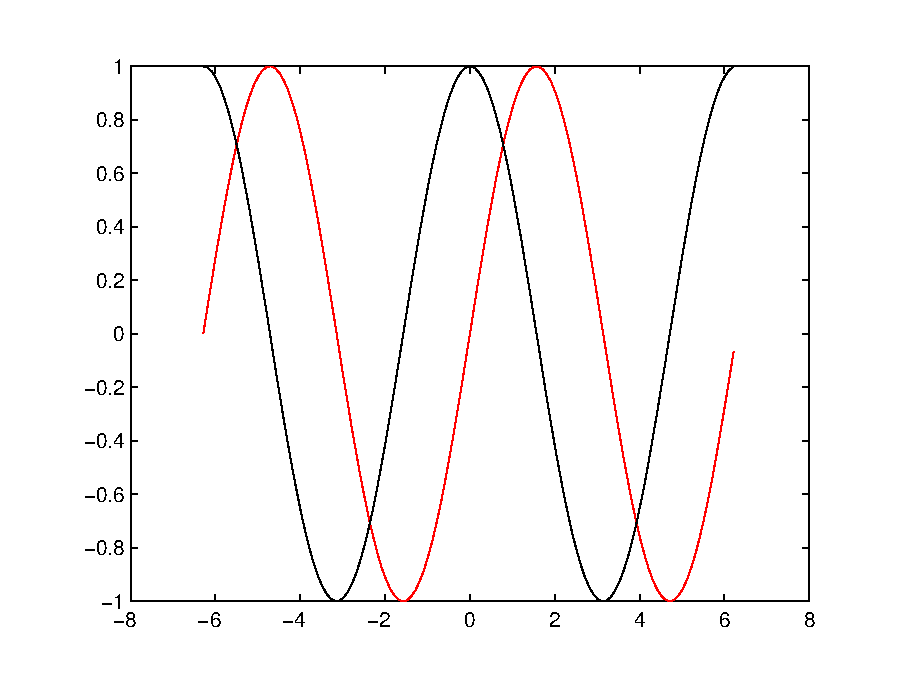
\includegraphics[width=\linewidth]{ch2-debug1.eps}
\caption{Output from the (bug-fixed version of) \textsf{plot\_some\_dull\_stuff} \textit{m-file}.}
\label{fig:ch2-debug1}
\end{marginfigure}

%------------------------------------------------

\newpage

%------------------------------------------------

\section{Functions}

\textit{Functions} in \textbf{MATLAB}, are really just fancy \textit{scripts}. Again -- just plain old lines of code in a text file that is given a \textsf{.m} extension (making it an \textit{m-file}). The big difference from a \textit{script} in MATLAB is that a \textit{function} can take variables as input and/or return variables (or variable values) as an output. (In contrast, a \textit{script} takes no input and returns no outputs, other than plots or data files that might be saved.) 

A \textit{function} is defined (and differentiated from a \textit{script}) by a special line at the \uline{very start}\sidenote{Literally: line 1. Not even a comment line is allowed to appear before the \textit{function} definition line.} of the \textit{m-file} (see Box). \uline{You must follow the \textbf{MATLAB} syntax exactly in defining a function.}

\marginnote{\begin{mdframed}[backgroundcolor=gray!10, roundcorner=10pt,leftmargin=1, rightmargin=1, innerleftmargin=5, innerrightmargin=5, innertopmargin=5,innerbottommargin=5, outerlinewidth=1, linecolor=light-gray]
\textit{\textbf{Functions}}
\\The all-important fancy first line of a \textit{function}, as defined in \textbf{MATLAB} help, looks like:
\begin{docspecmargin}
function [y1,...,yN] = myfun(x1,...,xM)
\end{docspecmargin}
Thanks \textbf{MATLAB} (this seems overly complex to say the least)!
\\OK -- lets break this down. Lets assume that you call the \textbf{m-file} calc\_stuff. The minimal definition of a function then looks like:
\begin{docspecmargin}
function [] = calc\_stuff()
\end{docspecmargin}
(The \textit{syntax} is critical and the definition line must look like this.) Here we are saying -- pass in not parameters and return no values either. So exactly like a normal script would work and you would execute the function calc\_stuff by typing at the command line:
\begin{docspecmargin}
>> calc\_stuff()
\end{docspecmargin}
(Maybe you can get away without the \texttt{()} bit.)
\\If you wan to pass in a single parameter (here: X), then you define the function:  
\begin{docspecmargin}
function [] = calc\_stuff(X)
\end{docspecmargin}
(To pass in more than 1 variable, simply comma separated the variable names.)
\\To pass out a parameter (here: Y) (and no input):
\begin{docspecmargin}
function [Y] = calc\_stuff()
\end{docspecmargin}
Lastly, at the end of the function, you include the line:
\begin{docspecmargin}
end
\end{docspecmargin}
\end{mdframed}}

This is all not as weird as you might think. For example, you have already used the \textit{function} \texttt{sin} -- this takes a single input (angle in radians), and returns a single output (the sine of the angle). If you were to write your own function for \texttt{sin}, the file would start something like:
\begin{docspec}
function [Y] = sin(X)
\end{docspec}
You can't, of course, go re-defining pre-defined \textbf{MATLAB} function names\sidenote{Actually you can, but it is best not to.}. So how about if in your work, you found you frequently needed to use the square of the sine of a number. You could keep writing:
\begin{docspec}
Y = (sin(X))\(^{\wedge}\)2
\end{docspec}
\noindent or, if you were a little more devious, you could create your own function for returning the square of the sine of a number. 

In this example, the contents of your \textit{m-file}, which here we'll call \textsf{sin2}\sidenote{And hence filename \textsf{sin2.m}.}, would look like:
\begin{docspec}
function [Y] = sin2(X)
\\Y = (sin(X))\(^{\wedge}\)2; 
\\end
\end{docspec}
\noindent but of course with \uline{lots} of comments to remind you what the \textit{function} does etc.

Your new \textit{function} is used pretty much as you would expect and have used previously, e.g.
\begin{docspec}
>> sin2(0.5)
\end{docspec}
\noindent will return the square of the sine of a value of 0.5 and dump the answer to the command line, and 
\begin{docspec}
>> Y = sin2(0.5);
\end{docspec}
\noindent does the same but assigns the answer to the variable \texttt{Y} (with the semi-colon suppressing output to the command line).

Go make up your own \textit{function} now. Start by creating one that takes a single input and returns a value equal to the sine of the square of the value (rather than the square of the sine as above). Test it (i.e. compare the output of your \textit{function} with the equivalent calculation typed in at the command line).

When you are happy with this, create one with 2 inputs (refer to \textbf{MATLAB} \texttt{help} on \texttt{function} and/or refer to the previous Box), that returns a value equal to the sine of the first input, divided by the cosine of the second input\sidenote{Mathematically, the answer is not valid for all possible values of the 2 inputs (why?), and later we'll learn how to pro-actively deal with such a situation.}, i.e.

\vspace{2mm}
\(y = \frac{sin(x_1)}{cos(x_2)}\))
\vspace{2mm}

You have used other \textit{functions}, perhaps without knowing it, and some of them return values, but because you have not attempted to assign the returned values to a variable, you may not have not noticed. For example, \texttt{plot} and \texttt{scatter} are in fact \textit{functions}, and return an ID of the plot graphic. We simply have not been asking for the returned value so far. As per \textbf{MATLAB} \texttt{help}:
\begin{docspec}
H = SCATTER(...) returns handles to the scatter objects created.
\end{docspec}
with the \texttt{handle}, \texttt{H}, being an identifier of the graphic which could prove to be useful if  e.g. you would like to modify  one of the properties of an existing graphic.

\marginnote{\begin{mdframed}[backgroundcolor=gray!10, roundcorner=10pt,leftmargin=1, rightmargin=1, innerleftmargin=5, innerrightmargin=5, innertopmargin=5,innerbottommargin=5, outerlinewidth=1, linecolor=light-gray]
\textbf{Debugging -- \textit{functions}}
\\\textit{Functions} are a prime example of the importance of being able to pause code part the way through (e.g. by setting a \textit{breakpoint}) because when a \textit{function} terminates, or crashes, you get to see none of the values of any variables created within the \textit{function}, unless they have been returned as output (and assuming here that the code did not crash and managed to get to the end). Setting a \textit{breakpoint} allows you to interrogate the values of any internal \textit{variables}.
\end{mdframed}}

Finally, it is important to note that by default, any variables created within a \textit{function} are TOP SECRET, and by that, I mean that they are not accessible to the main \textbf{MATLAB} workspace and do not appear listed in the \textsf{Workspace window}. To see that this is a non-Trumpian \uline{true fact}, create the following \textit{function} (basically, the first example but split into 2 steps):
\begin{docspec}
function [Y] = sin2new(X)
\\tmp = sin(X);
\\Y = tmp\(^{\wedge}\)2; 
\\end
\end{docspec}
\noindent Here, we have created a variable \texttt{tmp} to hold the value of the partial calculation. It does not appear in the \textsf{Workspace window} when you use the function. The advantage of this is that you could create a second function that also created a temporary variable internally called \texttt{tmp} with both instances of \texttt{tmp} treated entirely sperate and isolated by \textbf{MATLAB} (i.e. setting the value of one instance of \texttt{tmp} does not affect the value of the other).

The private nature of \textit{variables} created within \textit{functions} does however does lead to some additional complications in debugging \textit{functions} because when the function terminates, you have no record of what occurred during its execution (in terms of not being able to access the value of any of the variables used within the \textit{function}). Try setting a breakpoint at the start of the line where the square of \texttt{tmp} is calculated -- note that \texttt{tmp} now appears in the \textsf{Workspace window}. Continue the \textit{function} and when it terminates, note that \texttt{tmp} is now gone from the list.

%------------------------------------------------

\newpage

%------------------------------------------------

\section{Conditionals '101'}

%------------------------------------------------

\subsection{\texttt{if ...}}

One of the most important programming constructs is the \textit{conditional statement}, in which whether one or more \textit{statement}(s) are executed (and hence the overall outcome) is \uline{conditional} on the 'truth' or otherwise (i.e. it being true or false) of a given \textit{expression}.\sidenote{Pause ... and deep breath.}

\marginnote[-0.0in]{\begin{mdframed}[backgroundcolor=gray!10, roundcorner=10pt,leftmargin=1, rightmargin=1, innerleftmargin=5, innerrightmargin=5, innertopmargin=5,innerbottommargin=5, outerlinewidth=1, linecolor=gray!10]

\textbf{Conditional Statements}
\\The principal \textit{conditional statement} in \textbf{MATLAB} is: \docenvdef{if ... end}
\\The basic \texttt{if} structure is:
\begin{docspecmargin}
if EXPRESSION (IS TRUE)
\\ \ \ \ STATEMENT(S)
\\end
\end{docspecmargin}
in which the code \texttt{CODE} is executed if \texttt{EXPRESSION} is evaluated as \texttt{true}. No code is executed otherwise (and \texttt{STATEMENT} is \texttt{false}).

A variant addition -- \docenvdef{else} -- which allows for an alternative block of code (\texttt{OTHER STATEMENT(S)}) to be executed if \texttt{EXPRESSION} is instead evaluated as \texttt{false}, is:
\begin{docspecmargin}
if EXPRESSION (IS TRUE)
\\ \ \ \ STATEMENT(S)
\\else
\\ \ \ \ OTHER STATEMENT(S)
\\end
\end{docspecmargin}
Finally, there is 3rd variant including \docenvdef{elseif}:
\begin{docspecmargin}
if EXPRESSION (IS TRUE)
\\ \ \ \ STATEMENT(S)
\\elseif EXPRESSION (IS TRUE)
\\ \ \ \ OTHER STATEMENT(S)
\\else
\\ \ \ \ OTHER STATEMENT(S)
\\end
\end{docspecmargin}
Now, assuming that the first \textbf{EXPRESSION} is not true, a second \textbf{EXPRESSION} is evaluated, and only if that second \textbf{EXPRESSION} is also not true, will the final possible \textbf{STATEMENT} be evaluated. (Here, this final variant is shown with an \texttt{else ...} included at the end, but this is not a formal requirement to include.)

\end{mdframed}}

This is embodied in \textbf{MATLAB} (and similarly in most languages) by the \docenv{if ... end} construct (see \textit{Conditional Statements} Box).

In creating an \texttt{if ... end} construct, the statement tested for truth can be any one of:
\begin{enumerate}[noitemsep]
\setlength{\itemindent}{.2in}
\item A \textit{variable} having a value of \texttt{true} (\texttt{1}) or \texttt{false} (\texttt{0}). e.g.
\begin{docspec}
if happy
\\...
\end{docspec}
where \texttt{happy} is a variable.
\item A \textbf{MATLAB} \textit{function} returning a \texttt{true} or \texttt{false}, e.g.
\begin{docspec}
if isnan(A)
\\...
\end{docspec}
where variable \texttt{A}, may or may not be a \texttt{NaN}.
\item A \textit{relational operator} (see earlier), i.e. one of e.g.:
\begin{docspec}
>, <, <=, >=, ==, \(\sim\)=, \&\&, ||
\end{docspec}
and applied to a pair of \textit{variables}, one \textit{variable} and one value, or two values, e.g.:
\begin{docspec}
if A > B
\\...
\end{docspec}
where \texttt{A} and \texttt{B} are numbers.
\end{enumerate}

All this will hopefully become apparent during this and later weeks, so don't worry about the details ... just yet.

\vspace{1mm}
\noindent\rule{4cm}{0.5pt}

\newthought{An initial and rather computer programming textbook-like example} is as follows:

Designing a program (a \textbf{MATLAB} script saved as an \textit{m-file})  that asks whether or not you like bananas, and if you answer 'yes', tells you 'Correct -- they are a great fruit!'.

But before we worry about anything else (e.g. how to apply a \textit{conditional} statement), you'll  need to know about inputting information into a \textbf{MATLAB} program from the keyboard\sidenote{All programming languages have such a facility and man basic programs, at least in the Old Days prior to widespread \textit{GUI}s, make use of keyboard input}. Amazingly, you can guess (I actually just did) the command for requesting input -- it is \docenv{input} (for 'input' -- a rare occasion when everything is logical and simple!) (see Box).

Armed with this important new information (how to get \textbf{MATLAB} to ask for input and then receive and do something with keyboard input) -- firstly create a blank \textit{m-file} and save with a 'suitable' filename. Maybe add a header comment (1st line or lines starting with a \texttt{\%}) to remind you what this \textit{script} is going to do.

Secondly, (and on the next line) -- define the text (question) that you are going to ask and assign this string to the variable \texttt{MY\_QUESTION} (substitute your own filename here). Then place the input \texttt{command} (on the next, now 3rd line) for string input, and assign the input string to the variable \texttt{MY\_ANSWER}. You should have a program consisting of 3 (or more, depending on how much commenting you do) lines -- an initial comment line, a line defining the question and assigning this string to a handy variable (\texttt{MY\_QUESTION}), and a line taking the results of the input function, and assigning it to a second variable (\texttt{MY\_ANSWER}). The structure of your program should look like Figure \ref{fig:ch2-bananas}. To help you out, a complete program looks like:

\marginnote[-2.5in]{\begin{mdframed}[backgroundcolor=gray!10, roundcorner=10pt,leftmargin=1, rightmargin=1, innerleftmargin=5, innerrightmargin=5, innertopmargin=5,innerbottommargin=5, outerlinewidth=1, linecolor=light-gray]
\docenvdef{input}
\\There are two variants -- one for inputting numerical information and one for inputting a string (as\texttt{ 1 }could be either the value one or a 1-character string ...).
\\For inputting a numerical value:
\begin{docspecmargin}
X = input(PROMPT)
\end{docspecmargin}
will display the text in the string variable \texttt{PROMPT} and set the value of variable \texttt{X} to whatever number is entered (and after \textsf{RETURN} is pressed).
\\For inputting a string:
\begin{docspecmargin}
STR = input(PROMPT,'s')
\end{docspecmargin}
will display the text in the string variable \texttt{PROMPT} and set the value of \texttt{STR} when a string is entered (and after \textsf{RETURN} is pressed). Note that the second parameter passed to the function \texttt{input} (\texttt{'s'}), tells \textbf{MATLAB} that the input is a string rather than a number.
\end{mdframed}}

\begin{marginfigure}[0.0in]
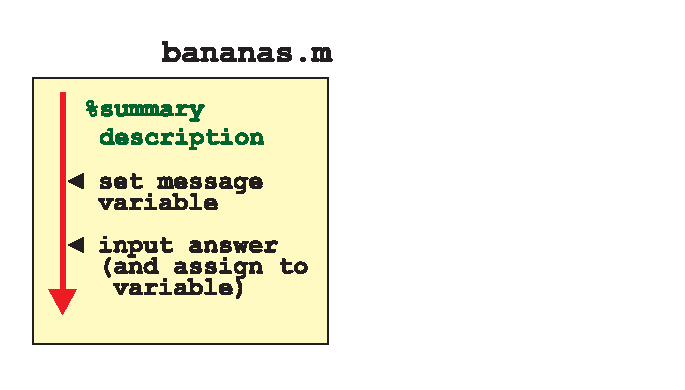
\includegraphics[width=\linewidth]{ch2-bananas.eps}
\caption{Schematic structure of the simple bananas question program.}
\label{fig:ch2-bananas}
\end{marginfigure}

\begin{docspec}
\textcolor[rgb]{0,0.501961,0}{\% === a program to ask whether I like bananas ===
\\\% first -- specify the question (and assign to a variable)}
\\var\_question\textcolor[rgb]{1,0,1}{ = 'Do you like bananas?'};
\textcolor[rgb]{0,0.501961,0}{\\\% now ... ask the question!}
\\var\_answer = input(var\_question,\textcolor[rgb]{1,0,1}{'s'});
\end{docspec}

Run the program thus far. You should see the question displayed, and when you type in an answer and hit \textbf{RETURN}, the program will end. Because your \textit{m-file} is configured as a \textit{script} and not a \textit{function} (see earlier), you can see the variable \texttt{MY\_ANSWER} in the variable list and you can hence check its value -- it should contain a \textit{string} with the answer you gave to the question. Make sure it all works like this so far.\sidenote{HINT: When you type the answer, it appears on the screen immediately adjacent (and untidily) to the end of the question. You can make this look nice(r) by adding a space at the end of the question string you assigned to prompt, e.g. \texttt{PROMPT = 'Do you like bananas? ';}.}

\vspace{1mm}
\noindent\rule{2cm}{0.5pt}
\vspace{2mm}

\noindent OK -- aside from the use of \texttt{input}, there is nothing new here. Yet. The ultimate purpose of the program is to give a reply that depends on the answer given. This is where we are going -- to utilize a \textit{conditional statement} -- depending on whether the answer is 'yes' or not, we are going to display a different message. This is a fundamental programming element -- different code (the \textit{statements} in the \textit{conditional} definition) will execute depending on the value of a \textit{variable} -- in this example, the 'different code' is a different message and the value of the variable is 'yes' or 'no' (or other answer).

You are going to add an '\texttt{if ...}' statement to the code (starting on line 4) to test whether the answer, held in the variable \texttt{MY\_ANSWER}, is equal to '\texttt{yes}'.
In the language of \textbf{MATLAB} syntax (see Box), the \textit{expression} is  whether the string contained in \texttt{MY\_ANSWER} is '\texttt{yes}'. How do we ask \textbf{MATLAB} to compare the value of \texttt{MY\_ANSWER} with '\texttt{yes}'?

Once upon a time, long long ago, \textbf{MATLAB} was simple and helpful and you could write:
\begin{docspec}
if (my\_answer == 'yes')
\\ \ \ [MESSAGE]
\\end
\end{docspec}

\noindent where \texttt{[MESSAGE]} you will later replace by a message that you will display using the \texttt{disp} command that you saw before. (In this stupid example it might be: 'Correct -- they are a great fruit!').
In this (now illegal!) usage, we are trying to ask whether the contents of the \textit{variable} \texttt{my\_answer}, are equivalent (the \texttt{==}) to the string \texttt{'yes'}.

\marginnote[-1.0in]{\begin{mdframed}[backgroundcolor=gray!10, roundcorner=10pt,leftmargin=1, rightmargin=1, innerleftmargin=5, innerrightmargin=5, innertopmargin=5,innerbottommargin=5, outerlinewidth=1, linecolor=light-gray]
\docenvdef{strcmp}
\\For once, the \textbf{MATLAB} help explanation is relatively simple and straightforward:

\textsf{tf = strcmp(s1,s2) compares s1 and s2 and returns 1 (true) if the two are identical. Otherwise, strcmp returns 0 (false).}

Which is pretty well much how we expected asking: \texttt{s1 == s2} to pan out.
\\(In \textbf{MATLAB} \textbf{help} -- \texttt{tf}, the variable name used in the example, is short for 'true-false'.)
\end{mdframed}}

Life is no longer this simple. \textbf{MATLAB} is going to make us use the function \docenv{strcmp} (see Box). In using \docenv{strcmp} we might break things down into 2 steps -- the first comparing the 2 strings (\texttt{MY\_ANSWER} and '\texttt{yes}') and returning to us a value of \textit{true} or \textit{false} that we will store in a new variable. In the second step, we'll ask the conditional to act on the value of the variable. The code will now look like this:
\begin{docspec}
COMPARISON\_RESULT = strcmp(MY\_ANSWER, 'yes');
\\if COMPARISON\_RESULT
\\ \ \ [MESSAGE]
\\end
\end{docspec}

Or, we could have made this more compact:
\begin{docspec}
if strcmp(MY\_ANSWER, 'yes')
\\ \ \ [MESSAGE]
\\end
\end{docspec}

Your code should now comprise something like the 3 lines from before (comment, define question, get input) followed by 4 lines of code of the conditional structure, comprising: the \texttt{strcmp} function, the \texttt{if ...}, use of \texttt{disp} to display a message, and lastly, \texttt{end}. The structure should look like Figure \ref{fig:ch2-bananas2}\sidenote[][-1.5in]{The red triangle denotes a branch point, where the code can go in different directions depending on the result of the \textit{conditional}. In this example -- there is only one branch, corresponding to the answer being 'yes'.} or if you assign the message to a 2nd variable, like Figure \ref{fig:ch2-bananas3}. A complete example program ... to help you follow all the above, would look like\sidenote[][-1.0in]{Note the \uline{indentation} of the contents of the \texttt{if ... end} structure. This is very common programming practice. You can make \textbf{MATLAB} do this for you by selecting a single line, or highlighting a block of lines, and clicking on the \texttt{Indent} icon in the code editor.}: 

\begin{marginfigure}[0.0in]
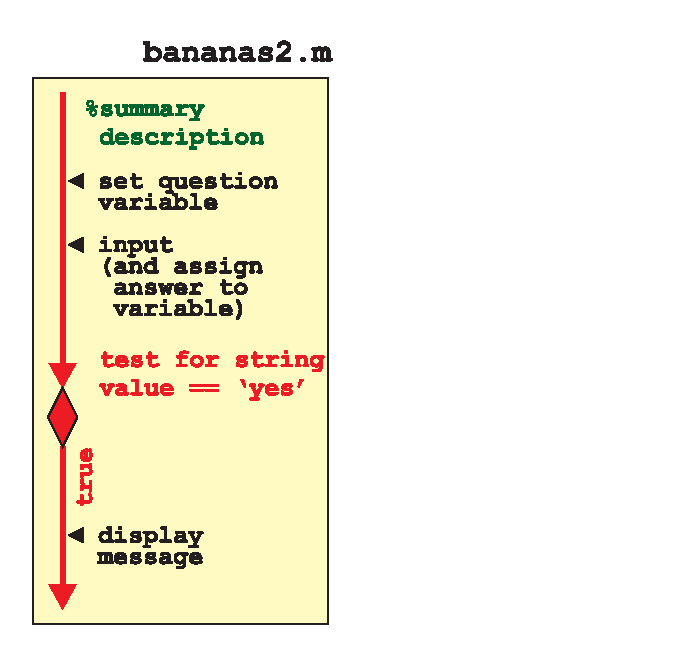
\includegraphics[width=\linewidth]{ch2-bananas2.eps}
\caption{Schematic structure of the extended bananas question program.}
\label{fig:ch2-bananas2}
\end{marginfigure}

\begin{docspec}
\textcolor[rgb]{0,0.501961,0}{\% === a program to ask whether I like bananas ===
\\\% === (and now give an answer!) =================
\\\% first -- specify the question (and assign to a variable)}
\\var\_question = \textcolor[rgb]{1,0,1}{'Do you like bananas?'};
\textcolor[rgb]{0,0.501961,0}{\\\% second -- specify the response (and assign to a variable)}
\\var\_response = \textcolor[rgb]{1,0,1}{'Me too! OMG I could die!'};
\textcolor[rgb]{0,0.501961,0}{\\\% now ... ask the question!}
\\var\_answer = input(var\_question,\textcolor[rgb]{1,0,1}{'s'});
\textcolor[rgb]{0,0.501961,0}{\\\% test the answer ... and reply if 'yes'}
\\\textcolor{blue}{if} strcmp(var\_answer, \textcolor[rgb]{1,0,1}{'yes'})
\\ \ \ \ disp(var\_response);
\\\textcolor{blue}{end}
\end{docspec}

\begin{marginfigure}[-0.0in]
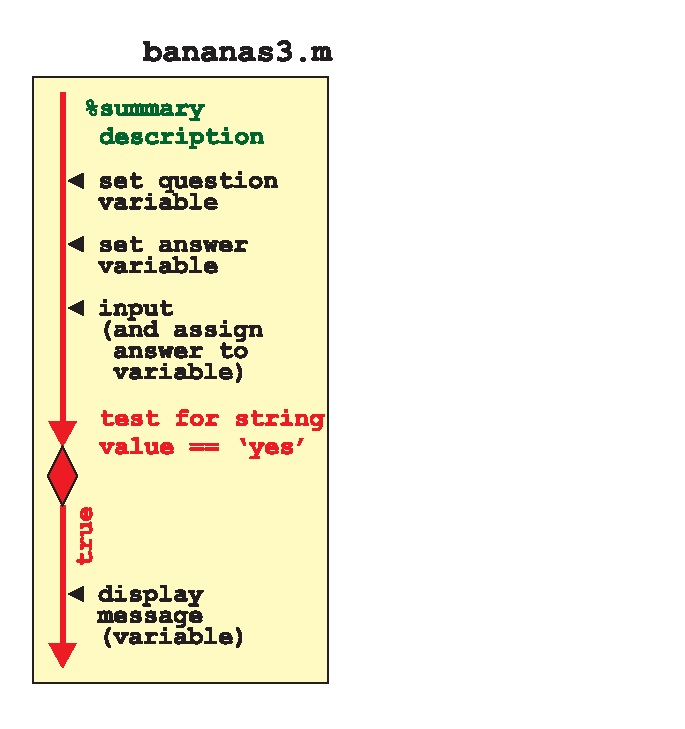
\includegraphics[width=\linewidth]{ch2-bananas3.eps}
\caption{A slight variant on the schematic structure of the extended bananas question program.}
\label{fig:ch2-bananas3}
\end{marginfigure}

\noindent(Please -- do not just copy-paste the code ... write your own code and only use, if you really need it, this code as a guide.)

Re-run (after saving) the program and confirm that it works (asking whether you like bananas and if you answer 'yes', tells you 'Correct -- they are a great fruit!'). If not -- time to de-bug! Note that if you tested the code in two stages, any bug at this point is only in the conditional structure. Start by double-checking the syntax required for the \texttt{if ...} structure. You could also try commenting out the message line and re-running.

You can also turn this around, and test for an answer that is not 'no' (the \(\sim\) is making the test, not 'no'), i.e.

\begin{docspec}
if \(\sim\)strcmp(MY\_ANSWER, 'no')
\\ \ \ [MESSAGE]
\\end
\end{docspec}

\noindent Now you are asking whether the answer is something other than 'no' (which might be 'yes', but not necessarily so) -- in the logical construct -- whether the (string) contents of \texttt{answer} are not equivalent to 'no'.

\vspace{1mm}
\noindent\rule{2cm}{0.5pt}
\vspace{2mm}

\noindent Next, you might display an alternative message is the answer is not 'yes'. Refer to \textbf{help} / the margin Box on if ... and note that you can extent the structure with an \texttt{else} which would be followed by a line displaying the alternative message (e.g. 'Then you need to get a life, apple-lover.')\sidenote{And then the line with \texttt{end} after that -- follow the prescribed structure *exactly*.}.

Try this first -- extend you program with an \texttt{else} line and then a an alternative message. The structure should now look like Figure \ref{fig:ch2-bananas4} and the code like:

\begin{docspec}
if strcmp(MY\_ANSWER, 'yes')
\\ \ \ [MESSAGE1]
\\else
\\ \ \ [MESSAGE2]
\\end
\end{docspec}

\begin{marginfigure}[+0.0in]
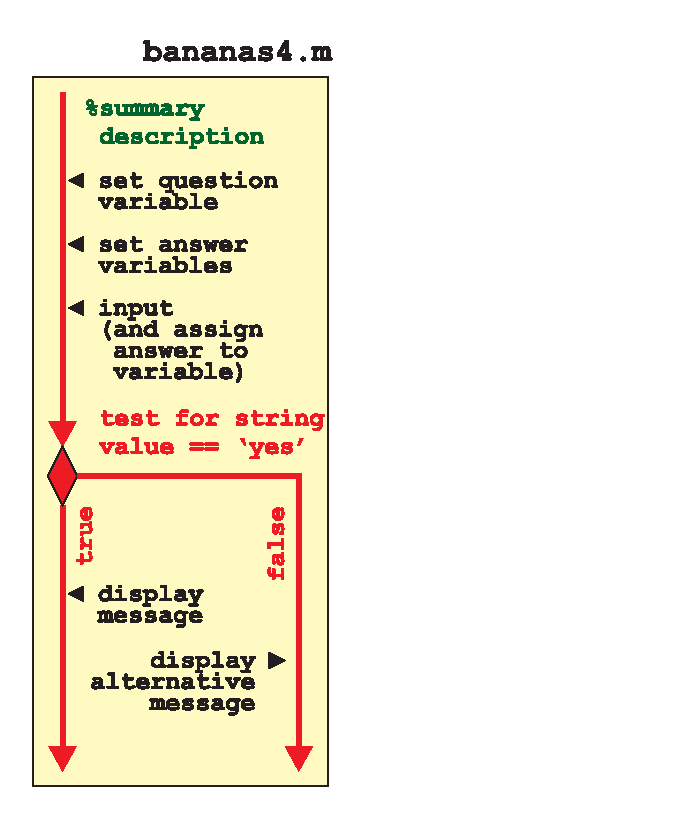
\includegraphics[width=\linewidth]{ch2-bananas4.eps}
\caption{Schematic of the bananas program using the \texttt{if ... else ...} construct (and displaying alternative messages).}
\label{fig:ch2-bananas4}
\end{marginfigure}

Finally -- you could extend this example further and tackle the situation of their being 3 possible answers -- 'yes', 'no', and ... 'I don't know' (or any other answer).
Now the basic structure becomes
\begin{docspec}
if strcmp(MY\_ANSWER, 'yes')
\\ \ \ [MESSAGE1]
\\elseif strcmp(MY\_ANSWER, 'no')
\\ \ \ [MESSAGE2]
\\else
\\ \ \ [MESSAGE3]
\\end
\end{docspec}
\noindent Here -- we are now adding an \texttt{elseif ... }line (followed by its specific message) (and see Box/\textbf{help}). Maybe try this and test it fully -- inputting a 'yes', a 'no', and some other answer, and confirming that you get the correct message displayed.

\vspace{1mm}
\noindent\rule{4cm}{0.5pt}

\newthought{Continuing to beat this same tired example to death ...} what if some wise-crack answered 'YES' rather than 'yes'?\sidenote{This goes to the heart of all software testing -- what if the user does something you were not expecting? Hence why all software undergoes extensive testing by user or people who did not test it. Sometimes there are pre-releases ('alpha' or 'beta' versions or simple 'pre-release') of software to all or specific parts of the user community, precisely to provide feedback, find bugs, and see whether they can break it ...} One could write:
\begin{docspec}
if strcmp(MY\_ANSWER, 'yes')
\\ \ \ [MESSAGE 1]
\\elseif strcmp(MY\_ANSWER, 'YES')
\\ \ \ [MESSAGE 1]
\\end
\end{docspec}
This will work, but you might note that you have had to exactly duplicate the MESSAGE line. If instead of displaying a simple message, a complex calculation was carried out -- all the lines of the code following the \texttt{if ...} would have to be exactly duplicated after the \texttt{elseif ...} . While it might seem trivial to simply copy-paste the required lines, this is\sidenote{Note quite in the same way that driving down a mountain highway with your eyes shut or hungry sharks are dangerous.} dangerous -- if the first set of lines are ever changed (due to a bug-fix or simple further development of the code), the same changes MUST\ then be exactly duplicated in each and every instance, or the code will not longer work correctly. This is *very* easy to forget to do, particularly for extensive code or code that you have not looked at for ... years. Code duplication also makes the overall code unnecessarily long (and hence harder to look through).

Instead, we can nest statements containing relational operators. What does this mean? Well, in the example of the answer being 'yes' or 'YES', logically, what we want is:

\begin{itemize}[noitemsep]
\setlength{\itemindent}{.2in}
\item[] (1) the contents of \texttt{answer} is equivalent to 'yes'
\item[] \ \ \ \ \ OR
\item[] (2) the contents of \texttt{answer} is equivalent to 'YES'
\end{itemize}
In code, this is written:
\begin{docspec}
strcmp(answer, 'yes') || strcmp(answer, 'YES')
\end{docspec}

Make sure you are happy with what this means (it is pretty well much exactly as it looks == logic).

So -- go modify your code to allow for a 'YES' or a 'yes'. Hell, try allowing for  a 'Y' or a 'y' as well.\sidenote{Sort of for this reason and that there are many different ways of writing 'yes', software often requires you to answer 'yes' in a restricted number of ways -- this restriction is made clear as part of the message that asks the question. Common is to restrict the answer to 'Y' or 'y'.} (You could extend it to 'no' also but I think you get the point ...) Be careful with all the nested parentheses -- an source of mistakes/bugs. You might write it like this, for example: 

\begin{docspec}
if (strcmp(answer, 'yes') || strcmp(answer, 'YES'))
\end{docspec}

\vspace{1mm}
\noindent\rule{4cm}{0.5pt}

\newthought{A non-text and non fruit related example. Almost.}

How many bananas could you eat in a day? I bet it is less than ten. We'll let the computer ask and if the answer is 10 or more, you (the computer) replies: 'liar!'.\sidenote{This example is even more stupid than the last one. But no more stupid than in any computer programming textbook and it will at least demonstrate a subtly different usage of \texttt{if ...}.}

The basic code is very similar to before. Create a new \textit{m-file}, add a comment line, define your question ('How many bananas do you think you could you eat in a single day?') and then get \textbf{MATLAB} to ask it and pass back whatever is entered in at the command line. The only difference at this point -- refer to the usage of \texttt{input} (see earlier Box) -- is that we want a number input rather than a string. You can call the \textit{variable} into which you assign the result of \texttt{input}\footnote{Note that the usage of \texttt{input}, now does not include the parameter \texttt{'s'} being passed (which previously specified that a \textit{string} input is expected).}, the same as before, or to make it distinct, e.g. \texttt{N\_BANANAS}, i.e.
\begin{docspec}
N\_BANANAS = input(MY\_QUESTION)
\end{docspec}

In the if statement, we now want to test whether the value of \texttt{N\_BANANAS} is greater or equal to 10 (or equivalently, greater than 9), i.e.
\begin{docspec}
if (N\_BANANAS >= 10)
\\ \ \ \ [MESSAGE1]
\\else
\\ \ \ \ [MESSAGE2]
\\end
\end{docspec}
or equivalently:
\begin{docspec}
if (N\_BANANAS > 9)
\\ \ \ \ [MESSAGE1]
\\else
\\ \ \ \ [MESSAGE2]
\\end
\end{docspec}

Write this code and get it going. Feel free to switch fruit / fruit consumption threshold, question/answers, or whatever.

%------------------------------------------------

\subsection{\texttt{switch ...}}

A slightly less commonly used alternative to \texttt{if ...} is:

\texttt{switch ... case ...} 

\noindent and is helpful in the case of multiple possible correct answers and/or multiple different answers.

\marginnote[-4.5in]{\begin{mdframed}[backgroundcolor=gray!10, roundcorner=10pt,leftmargin=1, rightmargin=1, innerleftmargin=5, innerrightmargin=5, innertopmargin=5,innerbottommargin=5, outerlinewidth=1, linecolor=gray!10]

\textbf{Conditional Statements (2)}
\\The other main \textit{conditional} statement is: \docenvdef{switch ... case ... end}
\\The basic \texttt{switch} structure is:
\begin{docspecmargin}
switch VARIABLE
\\ \ \ \ case VALUE(s)
\\ \ \ \ \ \ \ STATEMENT(s)
\\end
\end{docspecmargin}
which deviates rather from how \textbf{MATLAB} describes it, but this makes more sense to me (and hopefully to you). Here, \texttt{VARIABLE} is a variable and it is compared with one or more \texttt{VALUE(s)}. If the value of \texttt{VARIABLE} matches that of the \texttt{VALUE(s)}, then \texttt{STATEMENT(s)} are executed.

A common variant adds a default set of \texttt{STATEMENT(s)} to be executed if the value of \texttt{VARIABLE} does not match any of the \texttt{VALUE(s)}, e.g.
\begin{docspecmargin}
switch VARIABLE
\\ \ \ \ case VALUE(s)
\\ \ \ \ \ \ \ STATEMENT(s)
\\ \ \ \ otherwise
\\ \ \ \ \ \ \ STATEMENT(s)
\\end
\end{docspecmargin}

You can also have multiple case possibilities:
\begin{docspecmargin}
switch VARIABLE
\\ \ \ \ case VALUE(s)
\\ \ \ \ \ \ \ STATEMENT(s)
\\ \ \ \ case VALUE(s)
\\ \ \ \ \ \ \ STATEMENT(s)
\\ \ \ \ otherwise
\\ \ \ \ \ \ \ STATEMENT(s)
\\end
\end{docspecmargin}

\end{mdframed}}

For instance, and back to the ... fruit ... Consider the situation in which you want the same answer for multiple different kinds of fruit. Trying to code up the program that would give you 'A great fruit!' for any of 'banana', 'kiwi', 'apple', 'pineapple', and 'cucumber' (yes they are technically fruit -- \textbf{Google} it), you will find either that you have many lines of code and many duplicated lines of the same message, or a very long line after \texttt{if ...} with loads of \texttt{strcmp} and ORs (\texttt{||}).

Using \texttt{switch ... case ...} the code might instead look like:
 
\begin{docspec}
switch MY\_ANSWER
\\ \ \ \ case \{'banana', 'kiwi', 'apple', 'pineapple', and 'cucumber'\}
\\ \ \ \ \ \ \ disp('A great fruit!')
\\ \ \ \ otherwise
\\ \ \ \ \ \ \ disp('yuck!')
\\end
\end{docspec}

\noindent where \texttt{MY\_ANSWER} is the variable containing the name of a fruit entered in, in response to input, e.g.
\begin{docspec}
MY\_ANSWER = input('What is your favourite fruit?,'s');
\end{docspec}

Note that for a list of multiple possible values, \textbf{MATLAB} requires the list after \texttt{case} to be encased in curly brackets: \texttt{\{\}}. For a single answer, it would just be:
\begin{docspec}
\ \ \ case 'banana'  
\end{docspec}
for a string, and for a number:
\begin{docspec}
\ \ \ case 10  
\end{docspec}

\vspace{1mm}
\noindent\rule{4cm}{0.5pt}
\vspace{1mm}

\noindent Try re-formulating one of your earlier yes/no \texttt{if} questions in the form of a \texttt{switch ... case ...} code structure, with multiple possibilities for the form of e.g. a 'yes' dealt with by:

\vspace{-4mm}
\begin{docspec}
\\ \ \ \ case \{'YES', 'yes', 'Y', 'y'\}
\end{docspec}

%================================================

\newpage

%================================================

\section{Loops '101'}

%------------------------------------------------

\marginnote{\begin{mdframed}[backgroundcolor=light-gray, roundcorner=10pt,leftmargin=1, rightmargin=1, innerleftmargin=5, innerrightmargin=5, innertopmargin=5,innerbottommargin=5, outerlinewidth=1, linecolor=light-gray]
\textbf{\textit{loops} in \textbf{MATLAB}}

\docenvdef{for}
\\The basic \texttt{for ... end} structure is:
\begin{docspecmargin}
for n = VAL1:VAL2
\\ \ \ \ CODE
\\end
\end{docspecmargin}
\noindent where \texttt{VAL1} and \texttt{VAL2} are the limits that n will count between (starting at \texttt{VAL1} and ending at \texttt{VAL2}), meaning that \texttt{STATEMENT(S)} will be executed \texttt{(VAL2-VAL1)+1} times in total. \texttt{STATEMENT(S)} can be one or more lines of code, that will all be executed on each and every cycle of the loop.
\\The loop need not count in increments of one (1), the default, e.g.:
\begin{docspecmargin}
for n = VAL1:INC:VAL2
\\ \ \ \ CODE
\\end
\end{docspecmargin}
counts with an increment of \texttt{INC}. It is also possible to count down (a negative value of \texttt{INC}).

\docenvdef{while}
\\The basic structure is similar to that for \texttt{for ... end}:
\begin{docspecmargin}
while STATEMENT (IS TRUE)
\\ \ \ \ CODE
\\end
\end{docspecmargin}
\texttt{while} differs from \texttt{if} in that there are no alternative branches of code that can be executed. The \texttt{while ... end} loop cycles and \texttt{CODE} continued to be executed (for ever) until the \texttt{STATEMENT} is evaluated to be \texttt{false}.
\end{mdframed}}

The next main program construct that you are going to see is the \textit{loop}.
 There are a number of different forms of this in \textbf{MATLAB} (see \textit{loops} Box)  (and also in other programming languages), but the basic premise is the same -- a designated block of code (one of more lines of code\sidenote{It is possible to for the block of code to be only a fragment of a single line and hence the entire \textit{loop} plus code block, to be written on a single line.}), is repeated, until some condition is met. That condition might be something as simple as a count having been reached, e.g. the block of code is always executed  \textit{n} times, or the condition might be slightly more complex and involve a \textit{conditional statement} (see later). Will explore a very basic loop though an example, almost as contrived as for conditionals :o)

%------------------------------------------------

\subsection{\texttt{for ...}}

In this subsection we'll start with a very straight-forward and somewhat abstracted usage of \texttt{for ...}, which hopefully will get you in the mood for \textit{loops}. Then we'll go through some slightly more problem-focused examples.

\vspace{1mm}
\noindent\rule{4cm}{0.5pt}
\vspace{-2mm}

\newthought{Loops Ground Zero}. Basically -- \texttt{for} \textit{loops} cycle through a series of numbers between specific limits, or if you like, 'count' up (or down) through a series of numbers. As the loop counts (cycles), it allows you to execute some code, so for each count (or cycle), the (same) block of code is executed. We'll worry about what you might 'do'\sidenote{Note intentionally a joke. Actually, this is only funny if you know \textbf{FORTRAN}, and even then it is only marginally funny.} (i.e. the code fragment) in a \textit{loop}, later.

Consider, or rather: create a new \textsf{m-file}\sidenote{Comment it!}, and add following  code for a simple loop to the file:
\begin{docspec}
for n=1:10
\\end
\end{docspec}
Save it. Run it. What did it do?

I bet you have absolutely no idea! It actually cycled around ten times, counting from \texttt{n=1} through \texttt{n=10}, but you would not know it as there was no code within the loop to do anything and tell you anything about it.\sidenote{You get one clue -- if you look in the variables \textsf{Workspace window}, you'll see there is a \textit{variable} \texttt{n}, with a value of \texttt{10} -- the last value it was assigned before the \textit{loop} ended.}

There are 2 alternative but very crude debugging strategies you could take\sidenote{Plus, you could add a \textit{breakpoint} and view the value of n in the \textsf{Workspace window} each cycle around the loop.}:

\begin{enumerate}[noitemsep]
\setlength{\itemindent}{.2in}
\item Simply add a line \uline{within the loop} with the name of the (counting) variable, e.g.
\begin{docspec}
for n=1:10
\\ \ \ \ n
\\end
\end{docspec}
and it will spit out the value of \texttt{n} each time around the loop.
\item Or you can print the value of \texttt{n} 'properly'\sidenote{Although you can get away with just writing:
\begin{docspecmargin}
disp(n)
\end{docspecmargin}
}, e.g.
\begin{docspec}
for n=1:10
\\ \ \ \ disp(n)
\\end
\end{docspec}
You could tart this up further by creating a string that provides more explicit information back to you, which is when you really need to use \texttt{num2str}, e.g.
\begin{docspec}
for n=1:10
\\ \ \ \ my\_string = ['The value of n is: ' num2str(n)]
\\ \ \ \ disp(my\_string)
\\end
\end{docspec}
or if you are happy with more going on in a single line:
\begin{docspec}
for n=1:10
\\ \ \ \ disp(['The value of n is: ' num2str(n)])
\\end
\end{docspec}
(but they work the same -- check it).

\end{enumerate}

If you are not yet 100\% with \textit{concatenation} -- the '\uline{action of linking things together in a series}' (dictionary definition), what is happening in the line: 

\begin{docspec}
my\_string = ['The value of n is: ' num2str(n)]
\end{docspec}

\noindent is that you are taking the string \texttt{'The value of n is: '}, and the string equivalent of the numerical value of \texttt{n} (created via the use of \texttt{num2str}) and ... joining them together, one (\texttt{num2str(n)}) after the other (\texttt{'The value of n is: '}).

\vspace{1mm}
\noindent\rule{4cm}{0.5pt}
\vspace{-2mm}

\newthought{Loops in action}. So, consider the following (somewhat contrived) problem -- you want to be able to enter a series of numbers and return their sum (although equally one could perform and return all sorts of statistics).\sidenote{Obviously, one way to do this would be to enter the numbers into a file first, use the load function, and calculate the sum.} The basic code is simple and you can try it out by first creating a new (\textit{script}) \textsf{m-file}.

Using the other (numerical input) form of \texttt{input} (see earlier), the code for entering 2 numbers, one after the other, might look like this (although in practice, your code is full of helpful comments, right?):
\begin{docspec}
my\_question\ = 'Please enter a number: ';
\\A = input(my\_question);
\\my\_question = 'Please enter a number: ';
\\B = input(my\_question);
\\disp(['The sum of the numbers is:  ' num2str(A+B)]);
\end{docspec}

The first 4 lines you should be A-OK with, you have seen something very like this before. In the last line, again, 2 strings have been \textit{concatenated} by enclosing \texttt{'The sum of the numbers is:  '} and \texttt{num2str(A+B)} in a pair of brackets \texttt{[]}. The string representing the number sum is itself created by adding \texttt{A} and \texttt{B}, and then converting the resulting number into a string using \texttt{num2str} (see earlier). As always -- if you are happier breaking down the last line into its component parts, e.g.
\begin{docspec}
answer = A+B;
\\answer\_string = num2str(answer);
\\disp(answer\_string);
\end{docspec}
then please do! There is no particular computational penalty in \textbf{MATLAB} (at least, not at this stage) for creating as many variables as you like and breaking down code into multiple lines.

So far so good. But what if you wanted 4 numbers summed ...
\begin{docspec}
my\_question = 'Please enter a number: ';
\\A = input(my\_question);
\\my\_question = 'Please enter a number: ';
\\B = input(my\_question);
\\my\_question = 'Please enter a number: ';
\\C = input(my\_question);
\\my\_question = 'Please enter a number: ';
\\D = input(my\_question);
\\disp(['The sum of the numbers is:  ' num2str(A+B+C+D)]);
\end{docspec}

You can see whether this is going -- firstly that you are duplicating more and more lines of code as the number of numbers increases. Secondly, and we'll come to that in a moment -- what if the program does not know \textit{a priori} how many numbers you want to sum? Or do you need to write a program for every single possible number of numbers that you might need to input and process? An impossible and thankless task ...

You can see the code that is being repeated (here for input \texttt{x}):
\begin{docspec}
my\_question = 'Please enter a number: ';
\\x = input(my\_question);
\end{docspec}

If you bothered to read the margin box earlier, you'd known that this is exactly what a \textit{loop} can be used for. We therefore want something of the form:
\begin{docspec}
for n = 1:MAX\_N
\\ \ \ \ my\_question = 'Please enter a number: ';
\\ \ \ \ x = input(my\_question);
\\end
\end{docspec}

\noindent (noting that in your own code, \texttt{MAX\_N}, for instance, could be \texttt{4}).

The easy part is the configuration of the loop -- in the previous example with 4 inputs, we would write:
\begin{docspec}
for n = 1:4
\end{docspec}
and the \textit{loop} with go around 4 times as the counter \texttt{n} counts from 1 to 4 (\texttt{MAX\_N}) in increments of 1 (the default behavior of the \textit{colon operator}). Each time around the \textit{loop} the block of (2 lines of) code is executed and a number is inputted. But what is still missing? Try it exactly like this and see if you can see what is going on, or rather, not going on. If you think it is not working as expected -- try some debugging (i.e. adding one (or more) \texttt{disp} statements within the loop code, \uline{or} add a \textit{breakpoint} within the \textit{loop}).  See if you can come up with a solution once you see what the problem is. (Warning: the spoiler is in the margin.)

\marginnote[-1.75in]{
It should be apparent if you tried it out, that the value of \texttt{x} at the very end of the program, is equal to the last value you entered. In other words, each time you go around the loop you are over-writing the previous entered value and end up with nothing to sum at the end. There are two (or more) possibilities to solve this:
\begin{enumerate}[noitemsep]
\setlength{\itemindent}{.2in}
\item You could keep a \textit{running sum}. This would also avoid having to explicitly calculate a sum at the end, but you would not have saved the numbers as you went an no other stats would be possible.
\\You would do this by adding the inputted value to the existing value, i.e.
\begin{docspecmargin}
x = x + input(prompt);
\end{docspecmargin}
where \texttt{x} is the running total. What this says is: take the current value of \texttt{x}, add the value if the user input, and place the total back into the variable \texttt{x}. 
\\The only problem here ... is that \textbf{MATLAB} does not know what the very first value of x is -- i.e. the value before the loop start and that you then try and add \texttt{input(prompt)} to. The solution is to initialise the value of x before the loop starts, e.g.
\begin{docspecmargin}
x = 0;
\end{docspecmargin}
\item Alternatively, you could add the newly inputted number to the end of an existing vector. In this way, you end up recording all the values that were inputted. e.g.
\begin{docspecmargin}
y = [y input(prompt)];
\end{docspecmargin}
which says take the vector \texttt{y}, and add a further value (\texttt{input(prompt)}) to the end of it. At the end of the program (after the loop has terminated), you have to sum the contents of the vector \texttt{y}.

Or, to break it down:
\begin{docspecmargin}
z = input(prompt);\\
y = [y z];
\end{docspecmargin}
\end{enumerate} 
}

After having tried your own solutions, try out  both of the given alternatives (see margin) (assuming that one of them was not also your solution). Note that you are not given the complete code needed and some further debugging might be needed (but they do both work!).

Two things to be aware of in doing this:

\begin{enumerate}[noitemsep]
\setlength{\itemindent}{.2in}
\vspace{1mm}
\item If you set the maximum number of items quite high and then get bored and need to exit the program -- press the key combination \textsf{Ctrl-C} and \textbf{MATLAB} will exit your program (but leave \textbf{MATLAB} itself still running).
\vspace{1mm}
\item If you run the program a second time and use the \textit{vector} approach, something very odd starts to happen to the reported sum. This is because there already exists a \textit{vector} with the same name left over from the first time you ran the \textit{script} program. You can solve this (first try it out -- running the program several times in a row to see what happens) either by initializing the vector \texttt{y}, just like you did for \texttt{x} in the 1st solution, i.e.
\begin{docspec}
y = [];
\end{docspec}
(before the loop starts, of course), or you can clear the workspace using \texttt{>> clear all} (clears *all* variables), or clear just the problem variable (\texttt{y}) that will end up growing and growing and growing ... (\texttt{>> clear y}).  
\end{enumerate}

\vspace{-1mm}
\noindent\rule{4cm}{0.5pt}
\vspace{2mm}

A different and simpler way of looking at creating a running sum, or in the case below, incrementing the value of a variable within the loop is to consider creating an explicit counting variable, sperate form the loop counter. Recall:

\begin{docspec}
for n = 1:10\\
end
\end{docspec}

\noindent will simply loop around 10 times, as the \textit{loop} counter \texttt{n} is repeatedly incremented by 1 (the default increment of the colon operator), until it reaches a value of 10.

Create a new \textsf{m-file} and enter the following code:

\begin{docspec}
m = 0;\\
for n = 1:10\\
\ \ \ m = m+1;\\
end
\end{docspec}

\noindent What do you expect to happen to the value of m? Add some \texttt{disp} statements and print out the values of \texttt{n} and \texttt{m} (from within the \textit{loop}), each time around the \textit{loop}, or add one or more \textit{breakpoints} in the \textbf{MATLAB} code editor. Was this what you expected? Why? What about the following?

\begin{docspec}
m = 1;\\
for n = 1:10\\
\ \ \ m = m+1;\\
end
\end{docspec}

As abstracted and odd as it might seem now, later, this will all be important to understand. Please make sure you do!

\marginnote{You might note that you should not substitute the variable name \texttt{n}, for \texttt{m}, i.e. as in something like:
\begin{docspecmargin}
n = 0;\\
for n = 1:10\\
\ \ \ n = n + 10;\\
end
\end{docspecmargin}
Why? (Try it and see, even.)}

%------------------------------------------------

\subsection{Other loop configurations and usages}

In the previous examples, the \textit{loop} limits were fixed in the program itself -- you'd have to edit the \textit{script} code and re-save the file in order to be able to input and sum a different number of values. You could create a more flexible program by making the \textsf{m-file} a \textit{function} rather than a \textit{script}.\sidenote{There are other ways of adding flexibility to the loop count that we'll see shortly.} 

The idea here is to create a \textit{function} that takes a single input. This input will be the maximum \textit{loop} count. If the input variable was called \texttt{max\_count}, then the \textit{loop} structure would now look like:
\begin{docspec}
for n = 1:max\_count
\\ \ \ \ my\_question = 'Please enter a number: ';
\\ \ \ \ x = input(my\_question);
\\end
\end{docspec}

Referring to the previous lessons on \textit{functions} (as well as \textsf{help} if need be), create a \textit{function} that when you call it, e.g. like:
\begin{docspec}
>> function\_sum(5)
\end{docspec}
will request 5 inputs in turn, and at the end, display the sum.\sidenote{So in addition to the code fragment given, you need to define (at the top) and then end (at the bottom) a \textit{function}, you need to create a running sum, and then after the \textit{loop} finishes, display the sum.}

Also create a variant of this \textit{function}, and have it return the sum, rather than display it. i.e. this \textit{function} will now take as input, the number of numbers you wish to input, and will return the sum of those numbers.

Alternatively, you could write your program as a \textit{script} and before the loop starts,  ask for the number of values to be entered, passing this to the variable \texttt{max\_count}, with the loop then looking exactly like the above. In both cases you are substituting a fixed number (e.g. 4) for a variable that might contain any number.

\vspace{1mm}
\noindent\rule{4cm}{0.5pt}
\vspace{2mm}

\noindent Finally, in addition to a flexible \textit{loop} count maximum limit, the value of the increment in the count each time around the loop need not be one and it also need not start from 1. For example:
\begin{docspec}
for n = 10:10:100
\\ \ \ \ ...
\\end
\end{docspec}
is exactly equivalent in terms of the number of iterations carried out to
\begin{docspec}
for n = 1:1:10
\\ \ \ \ ...
\\end
\end{docspec}
and which is the same as the default behavior of the colon operator:
\begin{docspec}
for n = 1:10
\\ \ \ \ ...
\\end
\end{docspec}
The value of  the loop counter \texttt{n} simply differs by a factor of 10 at every iteration between the top and bottom two versions.

%------------------------------------------------

\subsection{Fun(!) worked examples}

(Only one example to date. And not necessarily even that fun.)

\vspace{1mm}
\noindent\rule{4cm}{0.5pt}
\vspace{-2mm}

\newthought{\textit{Loops}, camera, action!}\footnote{\textcolor{red}{\textbf{Example codes provided}}}\footnote{(at end of text)} (A more colorful example of \textit{loops} in action.) What we are going to do is (load and) plot a sequence of monthly data-sets and put them together to create a movie (animated graphic) to illustrate the seasonality of temperature in global climate. You will hopefully thereby better appreciate the value of constructs such as \textit{loops} in computer programming in saving you a whole bunch of effort and needless duplication of code. (Equally, you might not have wanted a movie as the end result, but simply a number of plots, all identical except in the specific array of data they were plotted from.)

First download all the monthly global surface temperature data-files on the  course webpage (there are 12 files to download)\sidenote{In scripting, it is also possible to automate downloading files from the internet.}. Then you are going to want to plot them all ... which would get desperately tedious if you had to do this at the command line 12 times. Think how much more of your life you would be wasting if the data were weekly. Or monthly data for 1972 through 2003, some 372 separate data-files ... You would never have time to go get a coffee ever again(?)

To make an animation, we need to make a series of frames, with each one being a different monthly temperature plot (in sequence; Jan through Dec). The files are rather conveniently named: \texttt{temp1.tsv}, \texttt{temp2.tsv}, ... \texttt{temp12.tsv}\sidenote{Don't worry about the \texttt{.tsv} file extension -- the file format is plain old text (ASCII) and could have instead been \texttt{.txt}.}. We should start by loading this little lot in. For the first file we could write:

\begin{docspecbold}
>> temp = load('temp1.tsv','-ascii');
\end{docspecbold}

or equally:

\begin{docspecbold}
>> temp(:,:) = load('temp1.tsv','-ascii');
\end{docspecbold}

Or if we wanted to save all the data in a 3D array, we could also write:

\begin{docspecbold}
>> temp(:,:,1) = load('temp1.tsv','-ascii');
\end{docspecbold}

Can you see that these statements are identical? Try them all out, just to be sure. The last form is really useful, because we can now go on and write:

\begin{docspecbold}
>> temp(:,:,2) = load('temp2.tsv','-ascii');
\end{docspecbold}

What you have done here is to load the January 2D (lon-lat) temperature distribution into the 1st 2D layer of the \texttt{temp} array, and then we have gone and created a second 2D layer on top of the first with the February climate data in it. Look at the \textbf{Workspace window} (or type \texttt{size(temp)}) -- you now have a 3D (94\(\times\)192\(\times\)2) array. Fancy! This is your first 3D array -- there is nothing really conceptually different from the 2D arrays that you have already been using, we simply have a 3rd index for the third dimension -- if it helps, \uline{you can think of a 3D array as being indexed by: row, column, layer}. 

You could go on and load in the March, April, etc data in a similar fashion, but you should be able to see a pattern forming here -- each filename differs only in the number at the end of its name and this number corresponds not only to the number of the month, but will also correspond to the layer index of the 3D array that you will create. This is something that a \textit{loop} could be used for while you go off for a coffee. So this is what we are going to do -- use a \textit{loop} to load in all of the files. So go back and delete the lines that load in the files, one-by-one.

\textbf{Create a new \textit{script} \textsf{m-file}.} Call it ... anything you like\sidenote{\texttt{bob\_the\_builder.m} counts as 'anything you like', but that looks pretty lame and it certainly won't help you remember what the script does if you came back to it sometime in the future.}. However, as well as appropriately naming your \textit{script} file, add a \textit{comment} on the first line of the file as a reminder to yourself of what it is going to do.

We first need to construct the \textit{loop} framework. We'll call the month number counter variable, \texttt{month}. Create a \texttt{for} \textit{loop} (with nothing in it yet) with \texttt{month} going from \texttt{1} to \texttt{12}.\sidenote{Don't forget to suitably comment what it is that the \textit{loop} does with a line (or even 2, but don't write a whole essay) beginning with a \%.} Refer to the course text (this document!), and/or the \textbf{MATLAB}  documentation, and/or the entirety of the internet, if necessary. The syntax (and examples) is described in full under \texttt{>> help for}. Save the script (\textsf{m-file}) and run it\sidenote{Typing: the \texttt{m-file} filename without the extension.}. What happens? Can you tell?

One way of following what is going on as \textbf{MATLAB} executes the commands within a script is to explicitly request that it tells you how it is getting on. You can use the function \docenv{disp} to help you follow what the program is doing (this is Old School debugging\sidenote{You can also add a \textit{breakpoint} within the \textit{loop} and thus can cycle through the \textit{loops} one-by-one, thereby being able to check the status of the variables within the loop and how they change from iteration to iteration.}). Within the loop, add the following line:

\begin{docspecbold}
disp(month)
\end{docspecbold}

\noindent and then save and re-run the \textit{script}. Now you can see how the loop progresses. This sort of thing can be useful in helping to \textit{debug} a program -- it allows you to follow a program's progress, and if the program (or \textbf{MATLAB} script) crashes, then at least you will know at what loop count this happened at, even if you are not given any more useful information by \textbf{MATLAB}. Only when you are happy that you have constructed a \textit{loop} that goes around and around 12 times with the variable \texttt{month} counting up from 1 to 12; comment out (\texttt{\textcolor[rgb]{0,0.501961,0}{\%}}) the printing (\texttt{disp}) line\sidenote{Note that by commenting out a line rather than completely deleting it, if you want to print out the loop count in the future, all you have to do is to un-comment the line, rather than type in the command all over again. This can be really useful if your debug command is long, or particularly if you have a whole series of lines that are required to report the information you want to know.} (unless you have grown rather attached to it) and move on.

We can construct filenames to load in by:
\begin{enumerate}[noitemsep]
\setlength{\itemindent}{.2in}
\vspace{1mm}
\item Forming a complete filename by \textit{concatenating} sperate strings. For example: 

\begin{docspec}
>> filename = ['temp' '1' '.tsv']
\end{docspec}

\noindent will create the filename  out of 3 components parts -- a common elements of all the filenames (\texttt{'temp'}), the number of the month (\texttt{'1'}), and the file extension (\texttt{'.tsv'}). 
\vspace{1mm}
\item Converting a number value of a (count) variable to a string (the \docenv{num2str} function), so instead of hard-coding in the string representing a number (\texttt{1} in this example), you convert from the value of a counter, e.g. \texttt{num2str(month)}.
\end{enumerate}

\marginnote[-0.0in]{\begin{mdframed}[backgroundcolor=gray!10, roundcorner=10pt,leftmargin=1, rightmargin=1, innerleftmargin=5, innerrightmargin=5, innertopmargin=5,innerbottommargin=5, outerlinewidth=1, linecolor=gray!10]
\docenvdef{num2str}
\\Converts a number to a \textit{string} (\texttt{s}), e.g.
\begin{docspecmargin}
s = num2str(N)
\end{docspecmargin}
where \texttt{N} is any number type variable.
\\\texttt{num2str} is useful in adding specific captions to plots (with caption text based on the value of a numerical variable) and in creating automated strings (e.g. filenames) within a loop.
\end{mdframed}}

This is where the role of the loop counter  (stored in the variable \texttt{month}) comes in. Each time around the loop,  the value of  variable \texttt{month} is the number of the month. All you have to do is to convert this value to a  \textit{string} and thereby automatically generate the correct month's filename each time (as per above).

Now add the following within the \textit{loop} in your script;

\begin{docspecbold}
filename = ['temp' num2str(month) '.tsv'];
\end{docspecbold}

and after it (still within the \textit{loop}) some debugging\sidenote{Or you can make use of a \textbf{breakpoint}.}:

\begin{docspecbold}
disp(filename)
\end{docspecbold}

\noindent just to confirm that appropriate filenames are being generated.

Save and run the \textit{script}. Satisfy yourself that you know what it is doing. Can you see that you are now automatically generating all the 12 filenames in sequence? And this only takes 3 lines of code total (not including the debugging line), compared with 12 lines if you had to write down all the 12 file names long-hand.
 
Now \textit{comment out} (or delete) the \texttt{disp(filename)} line, and add a new line to load in each dataset from the filename that is constructed each time the loop goes around.\sidenote[][-1.0in]{Remember that the load line goes inside the loop. (Why? Try writing it outside the loop (at the end) and see what happens if you like.)} e.g.\footnote{Alternatively, you could store all the data slices as you load them in and  rather than specifying the 1st, then 2nd, etc layer of the 3D array, here we are specifying the layer with an index equal to the contents (or value) of \texttt{month}, which, if you remember, counts up from 1 to 12 in the \textit{loop}.
\begin{docspecmargin}
temp(:,:,month) = ... load(filename,'-ascii');
\end{docspecmargin}
If youn run this coding variant and take a look at the \textsf{Workspace window} -- note that you have an array (\texttt{temp}) that has size 94\(\times\)192\(\times\)12.
}:

\begin{docspecbold}
temp(:,:) = load(filename,'-ascii');
\end{docspecbold}

\noindent Note that rather than specifying the filename explicitly in the load command, you are now passing the string contained in the variable \texttt{filename}. (Hopefully on the previous line of code within the loop, you have created the string value of \texttt{filename} ...) 

\vspace{1mm}
\noindent\rule{4cm}{0.5pt}
\vspace{2mm}

\noindent We'll now add some graphics.

\begin{marginfigure}[-0.0in]
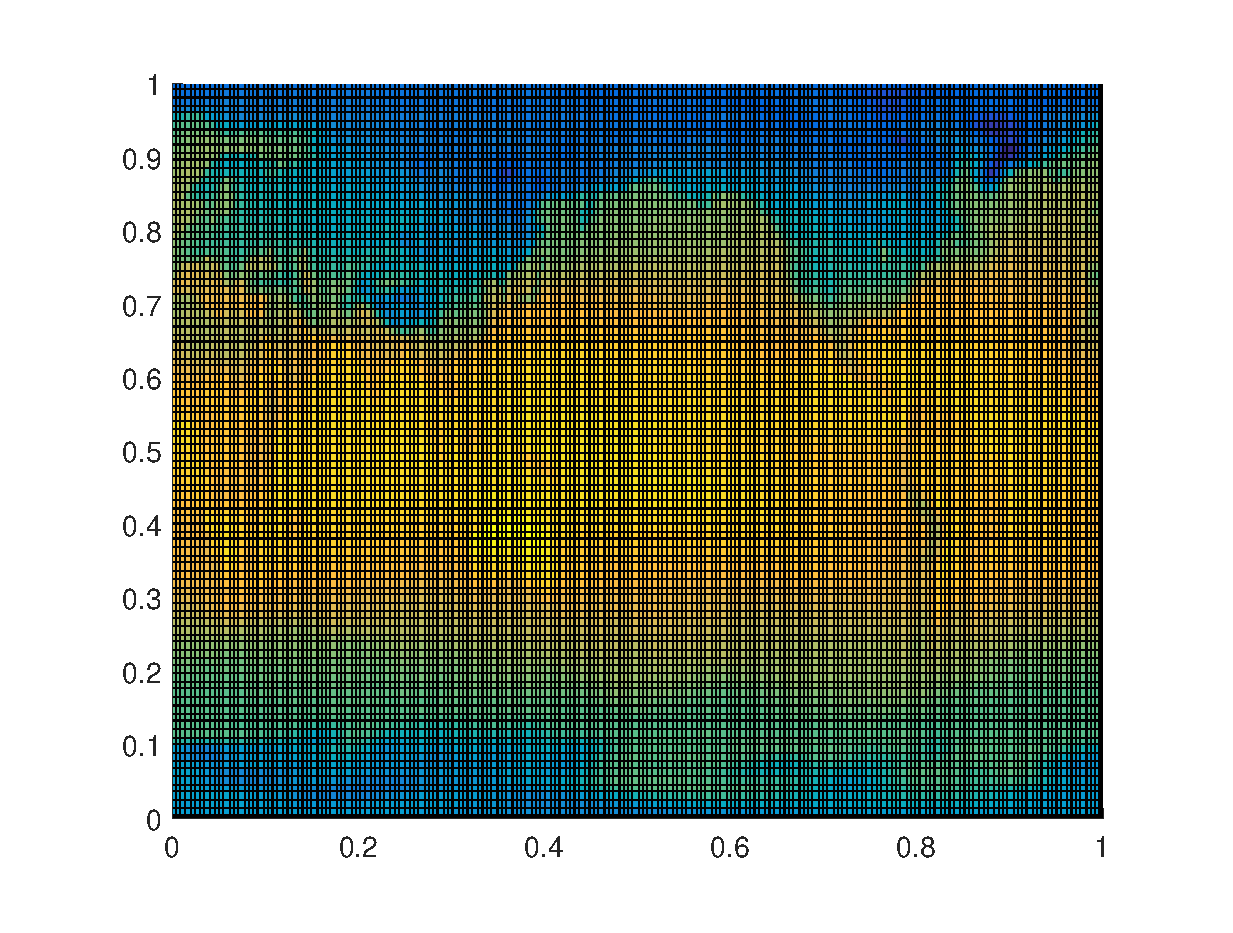
\includegraphics[width=\linewidth]{ch3-pcolortemp.eps}
\caption{Extremely unappealing blocky plot of Earth surface temperature (who cares with month? -- the graphics are too poor to matter ...).}
\label{fig:ch3-pcolortemp}
\end{marginfigure}

At the end of (but still within) the \textit{loop} (i.e., before the \textit{loop} has completely finished), create a new \textsf{figure window} and then plot (using \texttt{pcolor}) the monthly temperature data. On the subsequent lines, add the essential labelling stuff (lines after that). All within the loop still. These lines should look something like:

\begin{docspecbold}
figure;
\\pcolor(temp(:,:));
\end{docspecbold}

\noindent (or could be simply written \texttt{pcolor(temp);}) and should produce extremely exciting graphics as in Figure \ref{fig:ch3-pcolortemp}\sidenote[][0.25in]{The 2D graphics will get *much* better later -- one thing at a time!}.

Save and run the \textit{script}. Do you have 12 different temperature plots on the computer screen?\sidenote[][0.0in]{If not, stick you paw up in the air for help ...} Note that if you keep running the program, you'll get 12 more figure windows each time. This is where the \texttt{close all} command comes in useful, and you could add this at the start (or end) of your \textit{script}. Because if you re-run the \textit{script}, you wont then end up with 24 figure windows. And then 36 the time after that, and ... 

Actually, there is  no need to create a new \textsf{figure window} each time -- comment out the command that creates a new \textsf{figure window} (\texttt{figure}). Save and re-run and note the difference. 

\vspace{1mm}
\noindent\rule{4cm}{0.5pt}
\vspace{2mm}

\noindent Finally ... look up \textbf{MATLAB} \texttt{help} on \docenvdef{getframe}. Then go back to your global temperature loading/plotting script and add the following line to your program\sidenote{Where to put the line? Within the loop and after you have plotted the plot.}:

\begin{docspecbold}
M(month) = getframe;
\end{docspecbold}

Save and run. When \textbf{MATLAB} is all done, at the command line, type:

\begin{docspecbold}
>> movie(M,5,2)
\end{docspecbold}

\noindent and hopefully ... an animation of the progression of monthly surface air temperatures globally, should appear\sidenote{Note that the active Figure window may have disappeared behind some other windows so go rescue it to see what is happening.}.

If you want to play some more, just type \texttt{help movie} -- there are controls for not only the number of times you loop through the complete animation, but also for the numbers of frames per second. But we will revisit this later -- the 2D plotting you have done so far is *very* basic and there is no scale or sane x/y axes. Later we can also add the continental outlines that will help orient you and improve the quality of the graphical output. 

\uline{Before} you move -- go look at your \textit{script} -- is it well commented? Would you be able to tell exactly what it does it by the end of the course? What about next year? Are the \textit{loop} contents indented? It is important that it is commented and laid out adequately.

\vspace{1mm}
\noindent\rule{4cm}{0.5pt}
\vspace{2mm}

\noindent Creating a portable animation format would be useful (i.e. that you could play on a different computer or upload to the www). There is no longer a convenient \textbf{MATLAB} command to turn the \textbf{MATLAB} format movie (\texttt{M}) into a format you can use elsewhere (there used to be a command called \docenv{movie2avi} (see Box), but it has been ... retired (curse you, Mathworks)). The new/replacement command is \docenvdef{VideoWriter,} which differs mostly in that the animation is now created within the program and the  \textsf{.avi} format animation has its frames added (within the loop) as the graphics are created (rather than converting the frames afterwards as in \docenv{movie2avi}).

To use the \textbf{MATLAB} \docenv{VideoWriter} \textit{function}, you will need to adjust your code along the following lines   (and as per the \textbf{MATLAB} \textsf{help} on \docenv{VideoWriter})\footnote{Do not overly worry about the exact usage/syntax of \texttt{VideoWriter}.}:

\begin{docspecbold}
\textcolor[rgb]{0,0.501961,0}{\% Prepare the new file.}\\
vidObj = VideoWriter(\textcolor[rgb]{1,0,1}{'my\_animation.avi'});\\
open(vidObj);\\
\textcolor[rgb]{0,0.501961,0}{\% Create an animation.}\\
for month=1:12\\
\ \ \ filename = [\textcolor[rgb]{1,0,1}{'temp'} num2str(month) \textcolor[rgb]{1,0,1}{'.tsv'}];\\
\ \ \ temp = load(filename\textcolor[rgb]{1,0,1}{,'-}ascii');\\
\ \ \ pcolor(temp);\\
\ \ \ \textcolor[rgb]{0,0.501961,0}{\% Write each frame to the file.}\\
\ \ \ currFrame = getframe;\\
\ \ \ writeVideo(vidObj,currFrame);\\
end\\
\textcolor[rgb]{0,0.501961,0}{\% Close the file.}\\
close(vidObj);  
\end{docspecbold}

Note that the code above does not bother to create a 3D array of all the data loaded in, but rather, over-writes a 2D array (\texttt{temp}) each time around the loop (having first created the animation frame).
An animation is created at the end, but there is no record of all the 12 monthly datasets that were loaded in (and this may well be correct/the point).
(See the previous margin comment on how to modify things to create a 3D array of all the data.))\marginnote{\begin{mdframed}[backgroundcolor=gray!5, roundcorner=10pt,leftmargin=1, rightmargin=1, innerleftmargin=5, innerrightmargin=5, innertopmargin=5,innerbottommargin=5, outerlinewidth=1, linecolor=gray!5]
\textbf{\docenvdef{movie2avi}}
\\The function \docenv{movie2avi} converts an animation encoded in \textbf{MATLAB}'s \texttt{movie} format to an \textbf{avi} file, which is a common film format that can then be played in \textbf{Windows} (or other operating systems) without having to use \textbf{MATLAB} to display it. It is also a format that could e.g. be embedded in a \textbf{Powerpoint} presentation. A typical basic usage is:
\begin{docspecmargin}
>> movie2avi(M,'file.avi');
\end{docspecmargin}
\noindent where \texttt{file.avi} is the output filename and \texttt{M} the input \textbf{MATLAB} \texttt{movie} name.
\end{mdframed}}

%================================================

\newpage

%================================================

\section{Loops and conditionals ... together(!)}

%------------------------------------------------

No surprise that you might combine both \textit{loops} and \textit{conditionals} in the same programming structure. In fact, this becomes very powerful and is an extremely common device in programming. But this can all also become confusing ... remember to \uline{indent} your code.

\marginnote[-0.5in]{
\textbf{Indenting code}
\\Just do it (or let \textbf{MATLAB} do it).
Even for a single \textit{loop} or \textit{conditional}, it is way easier to see what code is within the \textit{loop} and what outside it, when the code inside starts several spaces in from the margin.
\\For nested \textit{loops} and \textit{conditionals}, it is even more important to keep (visual) track on what is going on.
\\Note that the indention (or lack of) does not affect the execution of the code (unlike in e.g. \textbf{Python}).
}

%------------------------------------------------

\subsection{\texttt{for ...} and conditionals}

Firstly, one might (rather trivially) use a conditional to decide whether to execute a loop 10 or 100 times, e.g.

\begin{docspec}
my\_string = input('Loop only 10 times (y or n)','s');
\\ if strcmp(my\_string,'y')
\\ \ \ \ for n = 1:10
\\ \ \ \ \ \ \ SOME CODE
\\ \ \ \ end
\\ else
\\ \ \ \ for n = 1:100
\\ \ \ \ \ \ \ SOME CODE
\\ \ \ \ end
\\ end
\end{docspec}

Here, we have a \textit{conditional} structure testing whether the string entered in response to the questions is 'y'. \texttt{If} 'y', then a loop of maximum count 10 executes, if not ('y') (\texttt{else}), then a loop of maximum count 100 executes.

This is a little messy and could be cleaned up and simplified somewhat. For instance -- by replacing the maximum loop count as a variable, whose value is set by the (\textit{conditional}) answer. e.g.

\begin{docspecbold}
my\_string = input('Loop only 10 times (y or n)','s');
\\ \textcolor{blue}{if} strcmp(my\_string,'y')
\\ \ \ \ n\_max = 10;
\\ \textcolor{blue}{else}
\\ \ \ \ n\_max = 100;
\\ \textcolor{blue}{end}
\\ \textcolor{blue}{for} n = 1:n\_max
\\ \ \ \ \textcolor[rgb]{0,0.501961,0}{\%}
\\ \textcolor{blue}{end}
\end{docspecbold}

\textbf{Enter in the second code (or some variant of it) into a new \textit{script} m-file, and explore how it works -- try changing the alternative loop limits, add a line within the loop to \texttt{disp} the value of \texttt{n} and hence confirm that the correct number of iterations of the loop occurs.} Note that you will need to replace \texttt{\textbf{\textcolor[rgb]{0,0.501961,0}{\%}}} with your own line (e.g. using \texttt{disp}) or you could have nothing and leave the comment \textcolor[rgb]{0,0.501961,0}{\%} line in. Remember to add comment lines.

\vspace{1mm}
\noindent\rule{4cm}{0.5pt}
\vspace{2mm}

\noindent Returning to the previous loop example concerning summing a series of numbers entered --  an alternative to (or as well as) a fixed \textit{loop}, or variable and (\textit{function}) parameter passed controlled \textit{loop}, we could specify a near infinite \textit{loop}, but provide a get out of jail free. For example, within the \textit{loop}, we could add a line that asks an additional question: 'Another input (y/n)?' We would test the answer and if no ('n'), exit the \textit{loop} (and report the sum as before). This would look like:
\begin{docspecbold}
\textcolor[rgb]{0,0.501961,0}{\% set up some strings for the 2 questions}
\\my\_question1 = 'Please enter a number: ';
\\my\_question2 = 'Another input (y/n)? ';
\\\textcolor[rgb]{0,0.501961,0}{\% initialize running sum}
\\running\_sum = 0.0;
\\\textcolor[rgb]{0,0.501961,0}{\% START OF LOOP}
\\\textcolor{blue}{for} n = 1:1000000
\\ \ \ \ \textcolor[rgb]{0,0.501961,0}{\% ask for a number}
\\ \ \ \ my\_number = input(my\_question1);
\\ \ \ \ \textcolor[rgb]{0,0.501961,0}{\% update running sum}
\\ \ \ \ running\_sum = running\_sum + my\_number;
\\ \ \ \ \textcolor[rgb]{0,0.501961,0}{\% display running sum}
\\ \ \ \ disp(['sum so far = ' running\_sum])
\\ \ \ \ \textcolor[rgb]{0,0.501961,0}{\% ask whether to keep going}
\\ \ \ \ my\_string = input(my\_question2,'s');
\\ \ \ \ \textcolor[rgb]{0,0.501961,0}{\% exit loop if answer is no}
\\ \ \ \ \textcolor{blue}{if} strcmp(my\_string,'n')
\\ \ \ \ \ \ \ \ break
\\ \ \ \ \textcolor{blue}{end}
\\\textcolor{blue}{end}
\\\textcolor[rgb]{0,0.501961,0}{\% END OF LOOP}
\end{docspecbold}

\noindent where \texttt{1000000} in the code is simply chosen as a 'very large number' and one rather larger than the maximum number of numbers you could ever imagine entering\sidenote{There us a better way of doing this, with the \texttt{while} construct, that we'll see shortly.}.

\marginnote[-0.0in]{\begin{mdframed}[backgroundcolor=gray!10, roundcorner=10pt,leftmargin=1, rightmargin=1, innerleftmargin=5, innerrightmargin=5, innertopmargin=5,innerbottommargin=5, outerlinewidth=1, linecolor=light-gray]
\docenvdef{break}
\\Simply -- \docenv{break} terminates the execution of a for or while loop'. And from \textbf{help} a further clarification: 'Statements in the loop after the break statement do not execute.'
\\Slightly more complicated (but not much) in the case of nested loops -- in this case, \texttt{break} exits only the loop in which it occurs.
\end{mdframed}}

The key new command here is \docenv{break}. The way the code works (hopefully!) is that towards the end of the \textit{loop}, the 'another input' question is asked -- if no further input is required, the loop exits via the \texttt{break} command. Remember  that now we have \textit{loops} and \textit{conditionals} nested together, it helps even more to \textit{indent} the code\sidenote{\textbf{MATLAB} will do this for you if you click on the Indent icon. It will also indent the code as far as it reasonably can, as you type.}. Also note that here -- the two different questions (demands) outputted to the screen -- 'Another input (y/n)?' and 'Please enter a number' -- are pre-defined before the \textit{loop} starts. These same text could equally  be placed directly within the \textit{loop} within the call to the \texttt{input} \textit{function}.

Currently, the program only exits upon entering 'n' to the question. Instead, we could have it exiting for any answer other than 'y':
\begin{docspec}
my\_question1 = 'Please enter a number: ';
\\my\_question2 = 'Another input (y/n)? ';
\\for n = 1:1000000
\\ \ \ \ my\_number = input(my\_question1);
\\ \ \ \ my\_string = input(my\_question2,'s');
\\ \ \ \ if \(\sim\)strcmp(my\_string, 'y')
\\ \ \ \ \ \ \ \ break
\\ \ \ \ end
\\end
\end{docspec}
which compares \texttt{my\_answer} and 'y', if this is not true (that they are the same), \texttt{break} is executed.

\textbf{Enter in the (highlighted) code into a new \textit{script} m-file and modify as per above, such that break is executed if any answer other than 'y' is entered.}

%------------------------------------------------

\vspace{1mm}
\noindent\rule{4cm}{0.5pt}
\vspace{-2mm}

%------------------------------------------------

\newthought{A practical example} of testing the value of a \textit{variable} and \texttt{break}-ing out of a \textit{loop} depending on the result of the test, would be when saving a data file. You might test for a filename  that already exists and if so, automatically modify the new file name so as not to over-write the existing file.\sidenote{Note that while in the \texttt{m-file} Editor, \textbf{MATLAB} asks you if you want to over-write an existing file, when saving a file directly from a program, no such dialogue box or warning is given.} The relevant function is \docenv{exist}, and in the case of a test for a file, the function returns either \texttt{0} (the file does not exist in the \textbf{MATLAB} search path, although that does not rule out it existing somewhere else entirely{}), or \texttt{2} (the file exists).

Clearly(?), in the example of saving the movie file, you might well want to test whether the filename that you have chosen already exists (i.e. the value returned by \texttt{exist} is \texttt{2}). If so (i.e. the file exists), you need to modify the filename  by means of a new concatenation, perhaps appending something like '\texttt{\_NEW}' to the end of the string\sidenote[][-0.75in]{Recall that in using the \texttt{movie2avi} command, you pass a filename -- simply modify the filename passed, in a similar way to in which you modified the filename for loading the temperature data.}. If not, and the filename has not already been used, you can proceed as before -- the equivalent of 'doing nothing'.
\marginnote[-0.5in]{\begin{mdframed}[backgroundcolor=gray!10, roundcorner=10pt,leftmargin=1, rightmargin=1, innerleftmargin=5, innerrightmargin=5, innertopmargin=5,innerbottommargin=5, outerlinewidth=1, linecolor=gray!10]
\docenvdef{exist}
\\Tests for whether a specified variable, function, file, or directory exists, and in generally, which is these it is.
\\The general syntax and usage is:
\begin{docspecmargin}
exist('A')
\end{docspecmargin}
to return what A is.
\\An extended syntax with a second passed parameter:
\begin{docspecmargin}
exist('A','file')
\end{docspecmargin}
returns value of \texttt{2} is returned is \texttt{A} if a file, and for: \begin{docspecmargin}
exist('A','dir')
\end{docspecmargin}
returns a value of \texttt{7} is returned is \texttt{A} if a directory.
\end{mdframed}}

You could start by defining a default filename in the code\sidenote{Either near the very start of the program (neater), or just before you need to use the string (to save a file).} that you will use if there is no clash with any existing file, e.g.
\begin{docspec}
my\_filename = 'GEO111\_movie.avi'
\end{docspec}
Now test whether this filename already exists:
\begin{docspec}
filename\_check = exist(my\_filename,'file')
\end{docspec}
Finally, using an \texttt{if} statement you are going to test whether the value of \texttt{filename\_check} is equal to 2. If so, you are going to need to modify the filename string (\texttt{my\_filename}). If not, you can let the \textit{conditional} just \texttt{end} and proceed to saving. Modifying the filename is just as per for the example of loading global temperature distributions, e.g.
\begin{docspec}
my\_filename = ['NEW\_' my\_filename];
\end{docspec}
where here, we take the string contained in \texttt{my\_filename}, we append a 'NEW\_' to the start\sidenote{Note that because the filename already has its \textsf{.avi} extension attached, you'll have to modify the start of the string.}, and assign the new (longer) string back into the variable \texttt{my\_filename}, like this:

\begin{docspec}
if filename\_check == 2
\\ \ \ \ my\_filename = ['NEW\_' my\_filename];
\\else
\\ \ \ \ \% DO NOTHING
\\end
\end{docspec}

\textbf{See if you can modify the \textsf{.avi} video creating code. An example code for the basic (non filename-checking) program is given at the end of the text. Create a new \textit{script} m-file with this code (or your own),  test whether it creates an animation successfully in the first place, and then try and modify it as per above with the filename check.} Hints: all the new code needs to go before the line:

\begin{docspec}
vidObj = VideoWriter('my\_animation.avi');
\end{docspec}

In this line,  the variable \texttt{my\_filename} that you have defined a default name in, will be passed instead of \texttt{'my\_animation.avi'}\footnote{Remember, you can pass a string directly, in which case \uline{it must be in inverted commas}, or you can pass the variable name. Do not place a variable name in inverted commas (or else the variable name itself will be interpreted as a string, when it is the contents of the variable you want).}, and the testing of whether your default filename already exists and whether to create a new(modified) filename, all comes before this. The order of the required lines of new of code is:

\begin{enumerate}[noitemsep]
\setlength{\itemindent}{.2in}
\item Set default filename.
\item Test whether this filename already exists and assign to the variable \texttt{filename\_check}.
\item Test whether the value of \texttt{filename\_check} is \texttt{2} and if so, modify the filename.
\end{enumerate}

%------------------------------------------------

\subsection{\texttt{while ...}}

We can re-frame the earlier example programs using the \texttt{while} construct rather than the \texttt{for} loop. But now ... you need to specify under what conditions the loop continues as the basic syntax (see earlier margin text on \textit{loops}, or \textbf{help}) is:

\begin{docspec}
while STATEMENT (IS TRUE)
\\ \ \ \ CODE
\\end
\end{docspec}

Here -- \texttt{STATEMENT (IS TRUE)} is the conditional. For instance and rather trivially, \textbf{create the following as a new \textit{script} m-file and run it}\sidenote{You ... are going to need a \textbf{Ctrl-C} on this one ...}:

\begin{docspecbold}
\textcolor{blue}{while} true
\\ \ \ \ disp('sucker')
\\\textcolor{blue}{end}
\end{docspecbold}

What has happened is that true is always ... true. Hence the condition is always met and the \texttt{while} \textit{loop}, loops forever. Conversely, \texttt{while false} would never \textit{loop}, not even once -- try it:

\begin{docspecbold}
\textcolor{blue}{while} false
\\ \ \ \ disp('sucker')
\\\textcolor{blue}{end}
\end{docspecbold}

More interesting and useful is when the statement might change in value as the loop progresses.

Think about the following code (and \textbf{type up in a new \textit{script} m-file and run it}):

\begin{docspecbold}
n = 0;
\\\textcolor{blue}{while} (n < 10)
\\ \ \ \ disp('sucker')
\\\textcolor{blue}{end}
\end{docspecbold}

This also will loop for ever as \texttt{n} is initialized to \texttt{0} and hence the statement \texttt{(n < 10)} is always true. But if we increment the value of \texttt{n} each time around the \textit{loop}: 

\begin{docspecbold}
n = 0;
\\\textcolor{blue}{while} (n < 10)
\\ \ \ \ disp('not a sucker')
\\ \ \ \ n = n + 1;
\\\textcolor{blue}{end}
\end{docspecbold}

\noindent then the \textit{loop} will execute exactly 10 times (just as per \texttt{for n = 1:10}) (\textbf{try this}).

You could also do the counting in reverse: 

\begin{docspecbold}
n = 10;
\\\textcolor{blue}{while} (n > 0)
\\ \ \ \ disp('not a sucker')
\\ \ \ \ n = n - 1;
\\\textcolor{blue}{end}
\end{docspecbold}

Now, \texttt{n} counts down from \texttt{10} and when it reaches a value of \texttt{0}, it is no longer greater than zero and the statement (\texttt{n > 0}) is false (and the loop terminates). \textbf{Also thy this modification, where the value of \texttt{n} counts down.}

It is not always completely obvious whether even simple while loops like this execute 9 or 10 (or 11) times particularly when often you might come across \texttt{while (n >= 0)} that allows the loop to continue when when \texttt{n} has reached z value of zero (but not below). \textbf{Spend a little while playing about with different \texttt{while} configurations and \textit{loop} criteria, adding \texttt{disp} lines or \textit{breakpoints} to find out how many times the \textit{loop} executes in total.}

Finally, note that the conditional statement in the \texttt{while} \textit{loop} need not test for an integer being larger or smaller than some threshold. One could equally loop on the basis of a string equality/inequality. For example, taking the previous example using \texttt{break}, the program could be re-coded using a \texttt{while} loop:
\begin{docspec}
my\_question1 = 'Please enter a number: ';
\\my\_question2 = 'Another input (y/n)? ';
\\my\_string = 'y';
\\ while strcmp(my\_string,'y')
\\ \ \ \ my\_number = input(my\_question1);
\\ \ \ \ my\_string = input(my\_question2,'s');
\\end
\end{docspec}
and ends up a slightly shorter and more compact piece of code, omitting the need for a \texttt{break} or a nested structure. Here, the 2 lines of \texttt{input} code will keep being executed, as long as the value of \texttt{my\_string} is \texttt{'y'}. Note that in this example, we  need to initialize the value of \texttt{my\_string} (to 'y' -- assuming that we want at least one number). \textbf{Try modifying (along the lines of the above) your previous code which was based on a \texttt{for} \textit{loop}, now using \texttt{while}.
}
%------------------------------------------------

\vspace{1mm}
\noindent\rule{4cm}{0.5pt}
\vspace{-2mm}

%------------------------------------------------

\newthought{Finally ... we could update the filename checking example ... using while.} The problem with the previous code is that you checked for the existence only a default filename (and appended '\textsf{\_NEW}' if a file already existed).

One (partial) solution would have been to, rather than append a pre-defined string ('\textsf{\_NEW}') to the filename,  request that the user provide  a completely new filename.

A complete solution would be to address the situation when asking for an alternative filename ... if that file existed too. We could keep checking for a filename clash and keep asking for a new filename, until a unique (unused) filename was provided by the user. Who knows how many attempts this might take (to find an unused filename), so \texttt{while ...} would be a better choice of loop than \texttt{for ...}. Because \docenv{exist} returns a \texttt{2} if the file already exists, a logical condition for \texttt{while}, would be that a filename determining \textit{loop} continues while \docenv{exist} is returning a value of \texttt{2}. e.g.

\begin{docspec}
my\_question = 'Enter a filename: ';
\\while (filename\_check == 2)
\\ \ \ \ my\_filename = input(my\_question,'s');
\\ \ \ \ filename\_check = exist([my\_filename],'file')
\\end
\end{docspec}

Within the \textit{loop}, a (new) filename is requested and then this string is checked against the directory contents. What is missing is the initial value of \texttt{filename\_check}. In a previous example, we simply set a value at the start. If we did that here, the first line of this code would look like: 

\begin{docspec}
filename\_check = 2
\end{docspec}

In this case, we do not need a default filename as the user provides a filename on the very first iteration of the loop.

\textbf{Try it out -- add the following code to the start of your basic avi file format saving movie program (e.g. as per at the end of the text), and use the value of the variable \texttt{my\_filename} as the name for saving the avi animation file and test it.}

\begin{docspecbold}
my\_question = 'Enter a filename: ';
\\filename\_check == 2;
\\\textcolor{blue}{while} (filename\_check == 2)
\\ \ \ \ my\_filename = input(my\_question,'s');
\\ \ \ \ filename\_check = exist([my\_filename],'file')
\\\textcolor{blue}{end}
\end{docspecbold}

%------------------------------------------------

\section{Even more (and loopier) loops}

[Further examples of increasingly extreme loopiness.]

%------------------------------------------------

\vspace{1mm}
\noindent\rule{4cm}{0.5pt}
\vspace{-2mm}

%------------------------------------------------

\newthought{Looping through arrays.} In plotting e.g. global temperature distributions, it would be nice to add on the continental outline on top. Currently, and particularly with the very  basic 2D plotting you have seen so far (\docenv{pcolor}), you are to some extent left guessing where the land and where the ocean is. We are going to work through using a loop to process data that define series of line segments that make up the outlines of the continents.\footnote{\textcolor{red}{\textbf{Example codes provided}}}

A pair of files are provided (from the website) that comprise a series of pairs of lon-lat values that delineate the outline of the continents and all but the smallest of islands:

\begin{itemize}[noitemsep]
\setlength{\itemindent}{.2in}
\item \textsf{continental\_outline\_lat.dat}
\item \textsf{continental\_outline\_lon.dat}
\end{itemize}

Download, and then load these into the \textbf{MATLAB} \textsf{workspace} (in the 'usual way'). You should now have 2 vectors. Maybe view them in the \textsf{Variable Window} to get a better idea of what you are dealing with. Also keep an eye on the entries in the \textsf{Workspace Window} and perhaps the \textsf{Min} and \textsf{Max} values to give you an idea of the range (here: of longitude an latitude values).

Try plotting these lon/lat locations. Use the \texttt{scatter} plotting function (which makes it all the easier as your data is in the form of 2 vectors already). You might need to reduce the size of the plotted points (refer to the earlier exercises, or \textsf{help}) and additionally, you might want to fill the points (up to you). Remember you can set the axis limits, which presumably should be 0 to 360 or -180 to 180, on the \textit{x}-axis (longitude), and -90 to +90 on the \textit{y}-axis (latitude). Font sizes of labels can also be increased if necessary. You might end up with something like Figure \ref{fig:ch3-continentaloutline}.
 
\begin{marginfigure}[0.0in]
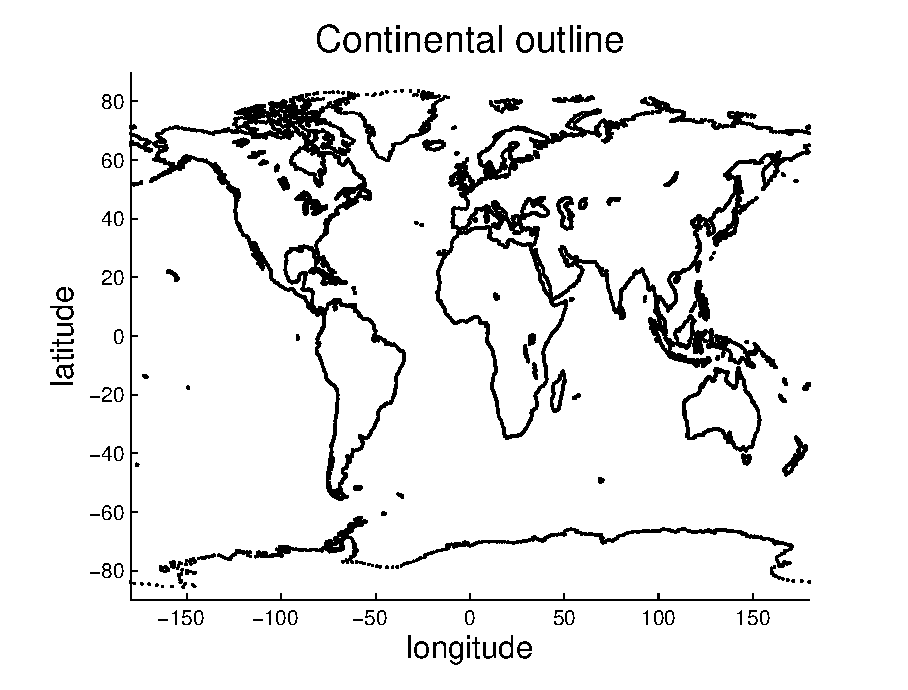
\includegraphics[width=\linewidth]{ch3-continentaloutline.eps}
\caption{Continental outline (of sorts).}
\label{fig:ch3-continentaloutline}
\end{marginfigure}

\textbf{You can try this at the command line} (no need at this point to put everything in a \textit{script} \textbf{m-file}):

\begin{docspecbold}
>> lon = load('continental\_outline\_lon.dat','-ascii');
\\>> lat = load('continental\_outline\_lat.dat','-ascii');
\\>> scatter(lon,lat);
\\>> axis([-180 +180 -090 +090]);
\\>> xlabel('longitude','fontsize',15);
\\>> ylabel('latitude','fontsize',15);
\\>> title('Continental outline','fontsize',18);
\end{docspecbold}

\noindent (but with lots of comment lines!).

By plotting dots (points), the coastal outline at higher latitudes gets increasingly pixelated (why?). So, we might instead plot as lines between the lon-lat pairs. For this, you could simply use \texttt{plot}. Do this, and see if you get something like Figure \ref{fig:ch3-continentaloutline2}.. 
\begin{marginfigure}[0.0in]
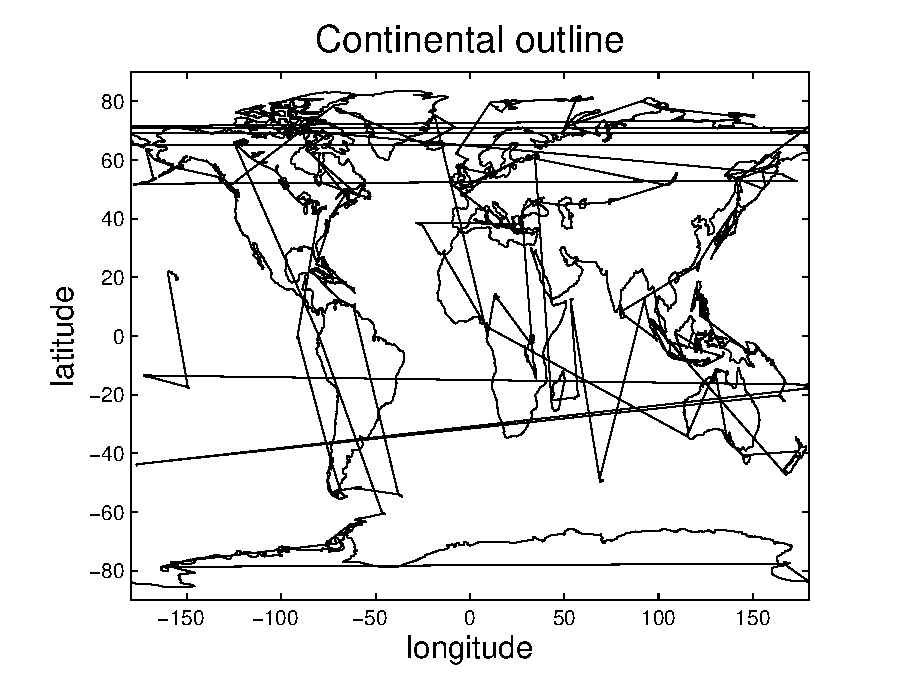
\includegraphics[width=\linewidth]{ch3-continentaloutline2.eps}
\caption{Another continental outline (of sorts).}
\label{fig:ch3-continentaloutline2}
\end{marginfigure}

Well ... interesting. If you think about it, as one continental outline is completed, the next lon-lat pair will be for the next continent or island. What \texttt{plot} does is to join up *all* the adjacent x-y (lon-lat) pairs and hence points, which is why you get the straight lines criss-crossing the map with  the start of each successive continent and island in the dataset joined to the end of the previous one.

The continental outline dataset is not actually that useless. There are  additional files that specify which block of lon-lat pairs belong to a single shape (i.e. continent or island). Load in the 2 additional files:

\begin{itemize}[noitemsep]
\setlength{\itemindent}{.2in}
\item \textsf{continental\_outline\_start.dat}
\item \textsf{continental\_outline\_end.dat}
\end{itemize}

i.e.:

\begin{docspecbold}
>> lstart = load('continental\_outline\_start.dat','-ascii');
\\>> lend = load('continental\_outline\_end.dat','-ascii');
\end{docspecbold}

\noindent(Note that you cannot simply call the second variable \texttt{end}.)

These vectors hold information regarding the start row and end row, of each shape. Again, view the contents of these vectors to get an idea of what is going on. For example, you'll see that the first entry is that the first shape starts on row \texttt{1} 
(\texttt{lstart}), and ends on row \texttt{100} (\texttt{lend}). The 2nd shape starts on row \texttt{101}, and ends on row \texttt{200}. etc etc

The simplest way too start dealing with all this, is to just plot the very first shape, defined by rows \texttt{1-100} of the lon and lat vectors. By now, you hopefully will be able to see that to plot rows \texttt{1-100} of  lon and lat data, you are going to do:
 
\begin{docspecbold}
>> plot(lon(1:100),lat(1:100));
\end{docspecbold}

Well ... this is probably about as unexciting as it gets -- a small piece of the Antarctic coastline. If you do a \texttt{hold on} and plot the next block (rows \texttt{101-200}), you'll get the next chunk of coastline. (Try this and see.) You could keep going this -- manually adding additional sections of the global continental outline. This could get tedious ... and it turns out that there are 283 different fragments to plot, all one after another. (This number comes from asking \textbf{MATLAB} the \texttt{length} of \texttt{lstart} or \texttt{lend}.) This is, of course, why we need to get clever with a \textit{loop} and automatically go through all 283 fragments, plotting them on on top of another in the same figure.

\marginnote{\begin{mdframed}[backgroundcolor=gray!10, roundcorner=10pt,leftmargin=1, rightmargin=1, innerleftmargin=5, innerrightmargin=5, innertopmargin=5,innerbottommargin=5, outerlinewidth=1, linecolor=gray!10]
\docenvdef{length}
\\This function could almost not be simpler -- just pass the name of a vector, and it returns its length (i.e. the number of rows, or columns, depending on the shape of the vector).
\end{mdframed}}

How? First you need to write the \texttt{plot} command in a more general form -- you do not want to have to read the values out of the \texttt{lstart} and \texttt{lend} files manually. Hopefully, it should be apparent that you can re-write the plot statement for the first fragment, as:

\begin{docspec}
plot(lon(LINE\_START:LINE\_END),lat(LINE\_START:LINE\_END));
\end{docspec}

where for the first fragment, the values of \texttt{LINE\_START} and \texttt{LINE\_END} are given by \texttt{lstart(1)} and \texttt{lend(1)}, respectively (renaming the original vectors to shorten the variable name)\sidenote{You cannot use the obvious variable name \texttt{end} -- why not?}. Re-writing again:

\begin{docspecbold}
>> plot(lon(lstart(1):lend(1)),lat(lstart(1):lend(1)));
\end{docspecbold}

Try this and check you still get the single piece of the Antarctic coastline.

Really, you should hopefully be making the mental leap to looking at \texttt{(1)} and thinking that it could be: \texttt{(n)}, where \texttt{n} is a loop counter which can go from 1 to 283\sidenote[][-0,0in]{This number comes from a 5th file -- \texttt{continental\_outline\_k.dat}, that numbers the continents/islands from 1 to 283. You don't need it, although downloading it, loading it, and determining the length f the vector gives you the loop limit and you would not have to go trusting me to write down 283 correctly without making a mistake ... } and hence loop through all the line fragments. Yes? For instance, setting \texttt{n=1}, and plot (with \texttt{n} replacing \texttt{1} in the code fragment above) -- you should again get that very  first fragment. Try setting \texttt{n=283} and plot. Do you get the last fragment (what is it of\sidenote[][1.0 in]{An island at about 20N and -150E if you have done it correctly.})?

So ...\textbf{ create yourself a new m-file}. Load in the lon-lat pairs as vectors (renaming then to something more manageable if you wish). Load in the vectors containing the start and end information. Create a \texttt{do ... end} loop. Maybe print (\texttt{disp}) the loop count and run the program (after saving), just to check first that the loop is functioning correctly. Before the loop, create a \textsf{Figure window}. and set \texttt{hold on}. You now have a basic shall of a program -- loading in the data, initializing a figure, and appropriate looping, but not yet actually doing anything within the loop.

In the \textit{loop} all you need is the \texttt{plot} command, but with the start and end rows being a function of \texttt{n} (or whatever you call the loop counter). Set axis dimensions and label nicely (after the loop ends). Run it. Hopefully ... something like Figure \ref{fig:ch3-continentaloutline3} appears(?)

\begin{marginfigure}[0.0in]
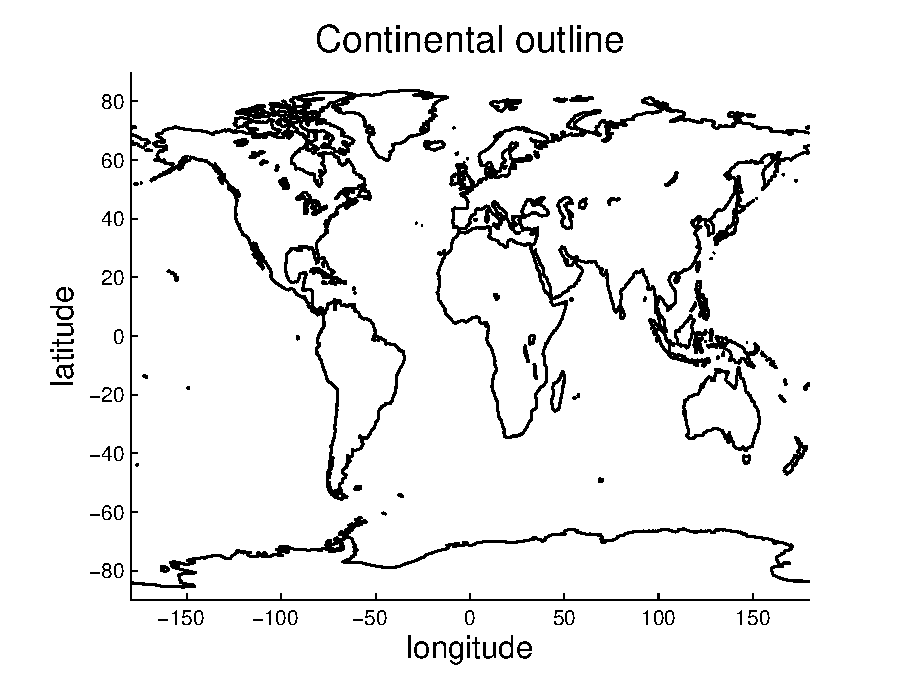
\includegraphics[width=\linewidth]{ch3-continentaloutline3.eps}
\caption{Another go at the continental outline!}
\label{fig:ch3-continentaloutline3}
\end{marginfigure}

An example code is given at the end of the text should you need any guidance as to e.g. in what order or where certain lines should go.

%----------------------------------------------------------------------------------------
% CHAPTER 3
%----------------------------------------------------------------------------------------

\chapter{Further ... MATLAB and data visualization}
\label{ch:03}

%------------------------------------------------
%
This chapter is something of a potpourri of \textbf{MATLAB} data and visualization methodologies and techniques, generally building on the basics covered in the previous chapters.

%------------------------------------------------

\newpage

%------------------------------------------------

\section{Further data input}

Previously, you imported ASCII data into \textbf{MATLAB} using the \texttt{load} command\sidenote{Or maybe 'cheated' and used the \textbf{MATLAB} GUI ...}. You might not have realized it at the time, but the use of \texttt{load} requires that your data is in a fairly precise format. \textbf{MATLAB} says "\textit{ASCII files must contain a rectangular table of numbers, with an equal number of elements in each row. The file delimiter (the character between elements in each row) can be a blank, comma, semicolon, or tab character. The file can contain MATLAB comments (lines that begin with a percent sign, \%).}" Firstly, your data may not be in a simple format and often may contain both numerical values and string values. Secondly, your data may not even be in a text/ASCII format. For instance, you data maybe be in an \textbf{Excel} spreadsheet, or for spatial scientific data, an increasingly common format is called '\textbf{netCDF}' (Network Common Data Form). In this section, we'll go through the basics and some examples of each.

Please regard this section as a simple overview on some of the different \textbf{MATLAB} file loading/input options (so that you know that they exist). For many one-off data loading problems, it can be easier to use the \textbf{MATLAB} GUI and the \textsf{Import Data} wizard. 

%------------------------------------------------

\subsection{Formatted text (ASCII) input}

The general procedure that you need to follow to input formatted text data is as follows:

\marginnote[-2.5in]{\begin{mdframed}[backgroundcolor=gray!10, roundcorner=10pt,leftmargin=1, rightmargin=1, innerleftmargin=5, innerrightmargin=5, innertopmargin=5,innerbottommargin=5, outerlinewidth=1, linecolor=light-gray]
\textbf{opening and closing files}
\\\textbf{MATLAB} has a pair of commands for opening and closing files for read/write:
\begin{itemize}[noitemsep]
\setlength{\itemindent}{.2in}
\item \docenvdef{fopen} will open a file. It needs to be passed the name (and path if necessary) of the file (as a string), and will return an ID for the file (assign (save) this  to a variable -- you'll need it!).
\item \docenvdef{fclose} ... will close the file. It requires the ID of the file (i.e. the variable name you assigned the result of calling \texttt{fopen} to) passed to it as a parameter. 
\end{itemize}
\end{mdframed}}

\marginnote{\begin{mdframed}[backgroundcolor=gray!10, roundcorner=10pt,leftmargin=1, rightmargin=1, innerleftmargin=5, innerrightmargin=5, innertopmargin=5,innerbottommargin=5, outerlinewidth=1, linecolor=light-gray]
\docenvdef{textscan}
\\According to (actually, paraphrased from) \textbf{MATLAB}:
\begin{docspecmargin}
C = textscan(ID,format)
\end{docspecmargin}
"\textit{ ... reads data from an open text file into a cell array, \texttt{C}. The text file is indicated by the file identifier, \texttt{ID}. Use \texttt{fopen} to open the file and obtain the \texttt{ID} value. When you finish reading from a file, close the file by calling \texttt{fclose(ID)}.}"
\\The \texttt{ID} part should be straightforward (if not -- follow through the Example).
\\The \texttt{format} bit is the complicated bit ... There is some help in a following Box and via the Example. Otherwise, there is a great deal of details and examples in \textbf{MATLAB help} -- you could look at this as a sort of menu of possibilities, and given a particular file import problem, the best thing to do is simply scan through help, looking for something that matches (or is close to) your particular data problem (and/or ask Google).
\end{mdframed}}

\begin{enumerate}[noitemsep]
\setlength{\itemindent}{.2in}

\item First, you need to 'open' the file -- the command (function) for this is called \docenv{fopen} (see Box). You need to assign the results of this \textit{function} to a \textit{variable} for later use.

What is going on and why this all differs so much form using \texttt{load}, where you only had to use a single command, is that you first have to open a connection to the file ... before you even read any of the contents in(!!!)\sidenote{This is very common across all(?) programming languages.}.

\item Secondly ... you can read the content in (finally!). The complications here include specifying the format of the data you are going to read in. You also need to tell \textbf{MATLAB} the ID of the file that you have opened (so it knows which one to read from) -- this is the value returned by the \textit{function} \texttt{fopen}. The \textit{function} you are going to use to actually read the data (having opened the file) is called \texttt{textscan}.

\item Once the data has been read it -- close the file using \docenv{fclose} (see Box). You are going to have to pass the ID of the  file again when you call this \textit{function} (so \textbf{MATLAB} knows which file to close).

\item Lastly, you are going to have to deal with the special data structure that \textbf{MATLAB} has created for you ...

\end{enumerate}

If you are interested (probably not) -- the connection made to an open file is called a file \textit{pipe}. Typically, you have have multiple open file \textit{pipes} at the same time in programs, and this is why obtaining and then specifying a unique ID for the \textit{pipe} you wish to read or write through, is critical.

\vspace{1mm}
\noindent\rule{4cm}{0.5pt}
\vspace{-2mm}

\newthought{As an initial Example} to illustrate this alternative (and more flexible) means of importing of ASCII (text) data, we are going to return to the paleo atmospheric CO\(_{2}\) proxy dataset file -- \textsf{paleo\_CO2\_data.txt}. Assuming that you have already (previously) downloaded it,  open it up in a text editor and view it -- you should see 4 neatly (ish) aligned columns of numeric values ... and 'nothing else'.

OK -- so having seen the format of the  data in the ASCII file, you are going to work through the following steps (you can do all this at the command line, or add the lines one-by-one to a \textit{script} m-file if you prefer)\sidenote{You can start off working at the command line if you wish, but ultimately, you are going to need to put everything into an \textbf{m-file}.}:

\begin{enumerate}[noitemsep]
\setlength{\itemindent}{.2in}

\item First 'open' the file -- you will be using the \textit{function}  \docenvdef{fopen}, and passing it the filename\sidenote[][-0.0in]{For convenience, you could assign the filename (+ its path) to a (string) variable and then simply pass the variable name -- remember, no \texttt{' '} needed for a variable naming containing a string (whereas \texttt{' '} is needed for the string itself).} (including the path to the file if necessary, i.e. if the \textbf{MATLAB} working directory does not also contain the file). So that you can easily refer to the file that you have opened later, assign the output of \docenv{fopen}\sidenote[][-0.0in]{The output is a simple integer index, whose value is specific to the file that you have opened.} to a variable, e.g.

\begin{docspecbold}
>> openfile\_id = fopen('paleo\_CO2\_data.txt');
\end{docspecbold}

\item Now ... this is where it gets a  trickier -- the \textit{function} you are going to use now is called \docenv{textscan}. Refer to \textsf{help} on \docenv{textscan}, but as a useful minimum, you need to pass 3 pieces of information:
\begin{enumerate}[noitemsep]
\setlength{\itemindent}{.2in}
\item The ID of the open file (you have assigned this to a handy variable (\texttt{openfile\_id}) already.)
\item The \textit{format} of the file (see margin note).(This is where it gets much less fun, but hang in there!) You simply list, space-separated, and between a single set of quotation marks, one format specifier per element of data.
\\In this particular Example, there are 4 items of data (per row) -- each of them is either an integer or a floating point number\sidenote{At least, none of them are clearly strings, right?}, depending on how you want to look at it. Assuming that the data is a floating point number, the \textit{format} for the input of each number item, is \texttt{\%f}.
\end{enumerate}
The result of \docenv{textscan} is then assigned to a parameter, e.g.

\begin{docspecbold}
my\_data = textscan(openfile\_id,'\%f \%f \%f \%f');
\end{docspecbold}

Here, the \texttt{'\%f \%f \%f \%f'} bit specifies that the data format consists of 4 floating point (real) numbers.

\item So far, so good! And you can now close the file:
\begin{docspecbold}
>> fclose(openfile\_id);
\end{docspecbold}

\marginnote[-1.0in]{\begin{mdframed}[backgroundcolor=light-gray, roundcorner=10pt,leftmargin=1, rightmargin=1, innerleftmargin=5, innerrightmargin=5, innertopmargin=5,innerbottommargin=5, outerlinewidth=1, linecolor=light-gray]
According to \textbf{MATLAB} \textsf{help}:
\\"\textit{the \texttt{format} is a string of conversion specifiers enclosed in single quotation marks. The number of specifiers determines the number of cells in the cell array C.}" Take this to mean that you need one format specifier, per column of data. The specifier will differ whether the data element is a number or character (and \textbf{MATLAB} will further enable you to create specific numerical types).
\\The format specifiers are all listed under \texttt{help textscan}. However, your Dummies Guide to \texttt{textscan} (and good for most common applications) is that the following options exist:
\texttt{
\\\%d -- (signed)integer
\\\%f -- floating point number
\\\%s -- string
}
\\\textbf{MATLAB} will automatically repeat the format for as many lines as there are of data. Alternatively you can specify precisely how many times you would like the format repeated (and hence data read in).
\end{mdframed}}

\item Actually, it does get darker before the light at end of the tunnel ... what \docenv{textscan} actually returns -- the data that was read in, is placed into an odd structure called a \textit{cell array}. It is not worth our while worrying about just what the heck this is, and if you view it in the \textsf{Variables} window (i.e. double click on the \texttt{cell array} name in the \textsf{Workspace} window), it does not display the simple table of 4 columns of data that maybe you were expecting. For now, we can transform this format into something that we are more familiar with using the \docenv{cell2mat} function, e.g.

\begin{docspecbold}
my\_data\_array = cell2mat(my\_data);
\end{docspecbold}

\end{enumerate}

And now ... it is done, i.e. there  exists a simple array, of 4 columns, the first being the age (Ma), the second being the CO\(_{2}\) concentration value (units of ppm), and the 3rd and 4th; minimum ad maximum error estimates in the proxy reconstructed value. :)

\marginnote[-1.0in]{\begin{mdframed}[backgroundcolor=gray!10, roundcorner=10pt,leftmargin=1, rightmargin=1, innerleftmargin=5, innerrightmargin=5, innertopmargin=5,innerbottommargin=5, outerlinewidth=1, linecolor=light-gray]
MATLAB claims that a \docenvdef{cell array} is "\textit{A cell array is a data type with indexed data containers called cells. Each cell can contain any type of data. Cell arrays commonly contain pieces of text, combinations of text and numbers from spreadsheets or text files, or numeric arrays of different sizes.}" I am sort of prepared to believe this.
\\Basically, in object-oriented speak, a cell array is an object, or rather, an array of objects. As \textbf{MATLAB} hints -- the cells can contain *anything*. Your limitation previously is that an array had to be all floating point numbers, all integers, or all strings, and if strings, all the strings had to be the same size. For strings in particular, it is obvious that a more flexible format where a vector could contain both 'banana' and 'kiwi' is needed (try creating a 2-element vector with these 2 words and see what happens). You clearly might also want to link a number with a string (e.g. number of bananas) in the same array, rather than have to create 2 sperate arrays.
\end{mdframed}}

\vspace{-1mm}
\noindent\rule{4cm}{0.5pt}
\vspace{-2mm}

\newthought{As a further example},  we are going to process a more complicated version of the paleo atmospheric CO\(_{2}\) proxy dataset. The file is called \textsf{paleo\_CO2\_data.dat} (rather than \textsf{.txt}) and is available from the course webpage. An initial problem here is even opening up the file to view it -- if you use standard \textbf{Windows} editors such as \textbf{Notepad} it fails to format it properly when displaying its contents\sidenote{If you use a \textbf{Mac} (or \textbf{linux}) however, all text editors should display the content jus fine.}. The first lesson then in scientific computing then is to have access to a more powerful/flexible editor than default/built-in programs such as \textbf{Notepad}. One good (\textbf{Windows}) alternative is \textbf{Notepad++}\sidenote{Conveniently installed on the Watkins computer lab computers.}. So go open the file with this instead\sidenote{Right-mouse-button-click over the file, then select \textbf{Open with} and then click on \textbf{Notepadd++}.}. Note the format -- there are a bunch of header lines and moreover, some of the columns are not numbers (but rather strings). So even if you were to manually edit out the headers with \docenv{comments} (\texttt{\%})\sidenote{Recall that \textbf{MATLAB} ignore lines starting with a \texttt{\%} and this includes loading in data lines using \texttt{load}.}, you are still left with the problem of mis-matched columns. You could edit the file in \textbf{Excel} to remove the problematic columns as well ... but now this seems like a real waste of time to be editing data formats with one software package just to get it into a second! (Again, you could use the \textbf{MATLAB} GUI import functionality
... but it will be a healthy life experience for you to do it at the command line :o) )

OK -- so having gotten an idea of the format of the ASCII data file, you are going to work again through the 4 steps:

\begin{enumerate}[noitemsep]
\setlength{\itemindent}{.2in}

\item First 'open' the file as you did before (using \docenv{fopen}) and assigned the ID returned by the function to a variable \texttt{openfile\_id2}.

\item Call \texttt{textscan}. However, we now want to pass 3 pieces of information (compared to 2 before):
\begin{enumerate}[noitemsep]
\setlength{\itemindent}{.2in}
\item The ID of the open file.
\item The \textit{format} of the data.
\item And now -- a parameter, together with an (integer) value, to specify how many rows of the file, assumed to be the header information, to skip.
\end{enumerate}

(Again -- the result of \docenv{textscan} is then assigned to a variable which will represent a \textit{cell array}.)

Lets do the easy bit first -- to tell \textbf{MATLAB} to skip \textit{n} lines of a file, you add the parameter \texttt{'HeaderLines'} to the list of parameters passed to \texttt{textscan}, and then simply tell it how many lines to skip. In this example:

\begin{docspec}
my\_data = textscan( ...
\\ \ \ \ \ \ openfile\_id2, ... ,'HeaderLines',3);
\end{docspec}

OK -- now to dive back into the \textbf{MATLAB} syntax mire ... Lets just load in just the first 2 columns of data, and assume that they are both integers (and skipping the first 3 lines of the file as per above). We might guess that we could simply write:

\begin{docspec}
my\_data = textscan( ...
\\ \ \ \ \ \ openfile\_id2,'\%d \%d','HeaderLines',3);
\end{docspec}

Try it (including closing the file, and a call to \texttt{cell2mat}, as before). What has happened?

It seems that \textbf{MATLAB} translates your format (\texttt{'\%d,\%d'}) into: 'read in a pair of integers, and keep automatically repeating this, until something else is encountered'. That something else is sequence of characters at the end of the first data line (line \#4, because we skipped the first 3), that makes \textbf{MATLAB} think that it has finished (or rather, that it cannot reading in 2 pairs of integers any longer). This leaves you with 2 pairs of integers -- i.e. a 2\(\times\)2 matrix (as you'll see if you look at \texttt{my\_data\_array}).

Here is a solution -- we could omit all the information following the first 2 elements (something for \textbf{Google} to help with).\sidenote{This turns out to be specifying \texttt{'\%*[\(^{\wedge}\)$\backslash$n]'}, which in effects sort of says:\\'skip everything (all the fields) (\texttt{\%*}) up until the end of the line is found (\texttt{[\(^{\wedge}\)$\backslash$n]}).}: 
\begin{docspec}
my\_data = textscan( ...
\\ \ \ \ \ \ openfile\_id2,'\%d \%d \%*[\(^{\wedge}\)$\backslash$n]','Headerlines',3)
\end{docspec}

The weird bit translates to ... \texttt{\%*} == ignore field ... until the line end == \texttt{[\(^{\wedge}\)$\backslash$n]}, and then read repeat for the next line.

(You are not expected to know or remember this nor be tested on it ... just to park at the back of your mind, that there are flexible ways of dealing with data input, including not reading everything in!)

\item Now you can close the file:
\begin{docspec}
fclose(openfile\_id);
\end{docspec}

\item ... and convert the results to something  human-readable:

\begin{docspec}
my\_data\_array = cell2mat(my\_data);
\end{docspec}

\end{enumerate}

This should do it -- a simple array, of 2 columns, the first being the age (Ma) and the second the CO\(_{2}\) concentration value (units of ppm). :)

\marginnote[-8.5in]{\begin{mdframed}[backgroundcolor=gray!10, roundcorner=10pt,leftmargin=1, rightmargin=1, innerleftmargin=5, innerrightmargin=5, innertopmargin=5,innerbottommargin=5, outerlinewidth=1, linecolor=light-gray]
\docenvdef{cell2mat}
\\Having created this weird format (\docenv{cell array}), now MATLAB has to give you a way of converting the data inside into something more usable. The function is \docenv{cell2mat}, which for a cell array C:
\begin{docspecmargin}
A = cell2mat(C);
\end{docspecmargin}
will return the corresponding ('normal') array A.
\\Now this is only true if all the data in \texttt{C} is of the same tpye (e.g. all floating point numbers). If the data types are mixed or you only wish for a sub-set of the data to be extracted and converted, simply index the required part of the cell array (Examples on this later).
\end{mdframed}}

The complete code (\textbf{enter into a new \textit{script} m-file and try it out}) looks like:

\begin{docspecbold}
openfile\_id2 = fopen('paleo\_CO2\_data.dat');
\\my\_data = textscan( ...
\\ \ \ \ \ \ openfile\_id2,'\%d \%d \%*[\(^{\wedge}\)$\backslash$n]','Headerlines',3);
\\fclose(openfile\_id);
\\my\_data\_array = cell2mat(my\_data);
\end{docspecbold}

There must be some sort of important life lesson hidden here. Perhaps about only working with well-behaved data files, or using the GUI import functionality? But hopefully it does illustrate that messy files can be dealt with, without the need for laborious editing or processing in \textbf{Excel}.

%------------------------------------------------

\subsection{Importing ... Excel spreadsheets}

If your data is contained in an Excel spreadsheet, and you want it in \textbf{MATLAB}, your options are:

\begin{enumerate}[noitemsep]
\setlength{\itemindent}{.2in}
\item Select some, or all, of the columns and rows in a specific worksheet, and either copy-paste this into a text file (but taking care that the worksheet column widths are formatted such that they are wider than the widest data element), or save in an ASCII format, with comma or tab delineations between columns. In either case, then load in the data using \texttt{load}, or if consisting of mixed numbers/text, go through the Hell that is \texttt{textscan} ....
\item Use \textbf{MATLAB} \textit{function} \docenv{xlsread}.
\end{enumerate}

\marginnote[-2.0in]{\begin{mdframed}[backgroundcolor=gray!10, roundcorner=10pt,leftmargin=1, rightmargin=1, innerleftmargin=5, innerrightmargin=5, innertopmargin=5,innerbottommargin=5, outerlinewidth=1, linecolor=light-gray]
\docenvdef{xlsread}
\\There are various uses (i.e. alternative allowed syntax) for \docenv{xlsread} for an \textbf{Excel} file with name \texttt{filename}. The 2 relevant and more useful ones look to be:
\begin{enumerate}[noitemsep]
\setlength{\itemindent}{.2in}
\item \texttt{num = xlsread(filename)}
which will return the *numeric* data in the Excel file \texttt{filename} in the form of a matrix, \texttt{num}. Note that non-numeric (e.g. string) headers and/or columns, are ignored. Also note that \texttt{num} is a 'normal' numeric array and does not require any conversion.
\item \texttt{[num,txt,raw] = ... 
\\ \ \ \ \ xlsread(filename)}
will additionally return text data in a \textit{cell array} \texttt{txt}, and *everything* in a cell array \texttt{raw}.
\end{enumerate}
You can also specify a particular worksheet out of an Excel file to load in:
\begin{docspecmargin}
num = ...
\ \ \ \ xlsread(filename,sheet)
\end{docspecmargin}
(and there are further refinements and options listed under \textbf{help}).
\end{mdframed}}

So ... option \#2 looks ... is looking the easiest ... :)

\vspace{1mm}
\noindent\rule{4cm}{0.5pt}
\vspace{-2mm}

\newthought{Returning to the paleo proxy CO\(_{2}\) data ...} but this time, as an \textbf{Excel} sheet. The data file you need is: \textsf{paleo\_CO2\_data.xlsx}
\\\noindent (You may as well go load this into \textbf{Excel} just to take a look at the format and so subsequently, you'll know if you have imported it faithfully or not.)

From the help box on \texttt{xlsread}, it should be pretty apparent what you do. And in fact, I am going to leave you to work it out -- try and import the age and CO\(_{2}\) data from \textsf{paleo\_CO2\_data.xlsx}.

Note that the simple usage of the \texttt{xlsread} \textit{function} gives you an \textit{array} containing just the numeric data. If you were to type:

\begin{docspecbold}
>> [num,txt,raw]=xlsread('paleo\_CO2\_data.xlsx');
\end{docspecbold}

\noindent then you sill get the numeric data returned in the array \texttt{num}, but you also get 2 cell arrays\footnote{
If you need to index a cell array, you do so pretty well much like a normal array, except it has an alternative syntax. For a normal, numeric array \texttt{A}, you might write:
\begin{docspecmargin}
>> A(4,3)
\end{docspecmargin}
to reference the value in the 4th row, 3rd column. For a \textit{cell array }\texttt{C}, to index the cell in the 4th row, 3rd column, you'd also write:
\begin{docspecmargin}
>> C(4,3)
\end{docspecmargin}
but you'd get a cell returned, not the value in the cell. If you want the value in the cell located at \texttt{(4,3)}, you'd put the index in curly brackets:
\begin{docspecmargin}
>> C\{4,3\}
\end{docspecmargin}
and you'd get a value of \texttt{3000} returned in this example.} -- \texttt{txt} and \texttt{raw}. \texttt{txt} contains just the text data, and \texttt{raw}, 'everything'. View these in the \textsf{Variable window} (by double-clicking on the variable names in the \textbf{MATLAB} \textsf{Workspace window}).

If you happen to have an \textbf{Excel} file with data (of any sort) in it from another class, practice loading in its contents into \textbf{MATLAB}. Note that if the \textbf{Excel} file contains cells with text in, you'll need to use the more advanced format of \texttt{xlsread} (see Box or \texttt{help}). Also try loading into only a single sheet of an \textbf{Excel} file (assuming the file has multiple sheets). 

%------------------------------------------------

\subsection{Importing ... netCDF format data}

Much of spatial, and particularly model-generated, scientific output, is in the form of \textit{netCDF} files. This is a format designed as a common standard to facilitate sharing and transfer of spatial data, but in a way that enables e.g. a 'complete' description of dimensions and various types of meta-data to be incorporated along with the data. The format is platform independent and a variety of graphical viewers exist for viewing and interrogating the data. Most programming languages support the reading and writing of \textit{netCDF} format data. \textbf{MATLAB} is no exception here.

\marginnote[0.5in]{\begin{mdframed}[backgroundcolor=gray!10, roundcorner=10pt,leftmargin=1, rightmargin=1, innerleftmargin=5, innerrightmargin=5, innertopmargin=5,innerbottommargin=5, outerlinewidth=1, linecolor=light-gray]
\docenvdef{ncread}
\\In its simplest incarnation:
\begin{docspecmargin}
data = ... ncread(filename,varname)
\end{docspecmargin}
where \texttt{filename} is the name of a \textit{netCDF} file, and \texttt{varname} is the name of the data variable in the \textit{netCDF} file.
\\e.g. if there was a variable called \texttt{rain} in the file \texttt{climate.nc},
\begin{docspecmargin}
data = ... ncread('climate.nc','rain')
\end{docspecmargin}
would read the values in the \textit{netCDF} file variable \texttt{rain} and assign to the variable \texttt{data}.
\\\textbf{MATLAB} provides a couple of further tricks, allowing you to read sections of the full \textit{netCDF} variable data array, or sample the data array -- see \textbf{help}.
\end{mdframed}}

\textbf{MATLAB} actually has a quick and simple, and ... a long-winded formal way of accessing data in a \textit{netCDF} file:

\begin{enumerate}

\item Using \docenv{ncread}, which reads data directly from the file.

\noindent \docenv{ncread} is by far the simplest way, although it lacks in flexibility and deviates from standard practices used across other programming languages.

\item Via a series of function calls to the netCDF library.

\noindent In the formal and more long-winded approach, you open the file and receive an ID for that file. The file can then be written to or read (including just interrogating its properties rather than necessarily extracting spatial data) using this ID. And of course, closed (using the same ID). The \textit{netCDF} standard is also little odd in how reading/writing is implemented and everything has to be done by determining the ID of a particular data variable or property of the file. 
The general approach is as follows:

\begin{enumerate}[noitemsep]
\setlength{\itemindent}{.2in}
\item Open the netCDF file by
\begin{docspec}
\textcolor{blue}{ncid} = netcdf.open(filename,'nowrite');
\end{docspec}
where \texttt{filename} is the name of the \textit{netCDF} file (which generally will end in \texttt{.nc}). \texttt{'nowrite'} simply tells \textbf{MATLAB} that this file is being open as read-only (this is the 'safe' option and prevents accidental deletion of over-writing of data).
\item This is the weird bit, as we cannot ask for the data we want automatically :o) Instead, given that we know\sidenote{There are ways of listing the variables if not.} the name of the variable we want to access, we ask for its ID\ ...
\begin{docspec}
\textcolor[rgb]{0,0.501961,0.25098}{varid}  = netcdf.inqVarID(\textcolor{blue}{ncid},NAME);
\end{docspec}
where NAME is the name of the variable (as a string), allowing us to then request the data:
\begin{docspec}
data  = netcdf.getVar(\textcolor{blue}{ncid},\textcolor[rgb]{0,0.501961,0.25098}{varid});
\end{docspec}
that says -- assign the data represented by the variable \texttt{\textcolor[rgb]{0,0.501961,0.25098}{varid}}, in the \textit{netCDF} file with ID \texttt{\textcolor{blue}{ncid}}, to the variable \texttt{data}.
\\So actually, not totally weird -- you request the ID of the variable, then use that to get access to the data itself. The names of the \textbf{MATLAB} commands vaguely make sense in this respect -- \texttt{inqVarID} for inquiring about the ID of a variable, and \texttt{getVar} for getting the variable (data) itself\sidenote{It is beyond the scope of this course to worry about why in the case of netCDF, the function are all \texttt{netcdf.} something. Just to say, it involves objects and methods and is a common notation in object orientated languages (that nominally, \textbf{MATLAB} isn't).}.
\item Finally -- close the file, by passing the ID variable into the function \texttt{netcdf.close}, i.e.
\begin{docspec}
netcdf.close(\textcolor{blue}{ncid});
\end{docspec}
\end{enumerate}

Note that you need to pass the ID of the \textit{netCDF} file for each and every command (after \texttt{netcdf.open}) so that \textbf{MATLAB} knows which \textit{netCDF} object you are referring to (you are allowed to have multiple \textit{netCDF} files open simultaneously).

\end{enumerate}

\vspace{-1mm}
\noindent\rule{4cm}{0.5pt}
\vspace{-2mm}

\newthought{For a \textit{netCDF} Example}, we'll take the output of a low resolution climate model. To start off, download the '2D marine sediment results' \textit{netCDF} file -- \textsf{fields\_sedgem\_2d.nc}. The data here is relatively simple -- a 2D distribution of bottom-water and surface sediment properties, saved at a single point in time. In other words, there are only 2 (spatial) dimensions to the data\sidenote{Adding time would make it 3 dimensions (2 spatial + 1 of time). Adding height or depth in the ocean would also make it 3 (3 spatial). 3 spatial + time would make for a 4-dimensional dataset ...}.

OK -- we'll start by opening the file. The ID\ of the variable we want to extract and plot  is called \textsf{'grid\_topo'}. To load/extract the 2D field and assign it to a variable \texttt{data}:

\begin{docspecbold}
>> data2d = ncread('fields\_biogem\_2d.nc','grid\_topo');
\end{docspecbold}

You should now have an array called \texttt{data}. It should be 36\(\times\)36 in size. \textbf{Plot it}\sidenote{Your choice of 2D plotting function that you have already come across, e.g. \texttt{pcolor} or \texttt{image}, although not all work as well on this particular dataset (e.g. the auto scaling in \texttt{image} causes issues).}. Can you deduce what it might be of? Is it in the correct orientation? (If not -- correct it, by rotating the array, and/or flipping the rows or column.)

(There are more appropriate ways of plotting this, which we will encounter later.)\footnote{Missing here are the x and y axis values, which you should have correctly deduced are longitude and latitude, respectively, with latitude presumably going from -90 to 90N, and longitude ... well, maybe it is not completely obvious exactly what the value of longitude is at the original.

A great strength of \textit{netCDF} its the ability of this file format to also contain the grid (axis) details that the data is on. There are ways of finding out the names of the axis variables (dimensions), but for now, I'll give you them:
\begin{itemize}[noitemsep]
\setlength{\itemindent}{.2in}
\item \texttt{'lat'} -- is the latitude axis. (Technically, the axis values are the mid-points of the grid cells.)
\item \texttt{'lon'} -- is the longitude axis.
\end{itemize}

The axes are held in the \textit{netCDF} file as vectors and we can retrieve this (1D) data in a similar way to the 2D data:
\begin{docspecmargin}
varid  = netcdf.inqVarID(ncid,'lat');
\\lat \ \ = netcdf.getVar(ncid,varid);
\\varid  = netcdf.inqVarID(ncid,'lon');
\\lon \ \ = netcdf.getVar(ncid,varid);
\end{docspecmargin}
in which we obtain the ID of the axis variable \texttt{'lat'}, then retrieve the axis data and assign it to a vector \texttt{lat} (and then likewise for longitude). Do this, and confirm that you get plausible vectors representing positions along a longitude and latitude axis.

The final task would then be to take the 2 axis vectors, and create a pair of matrices -- one containing longitude values associated with the 2D data points, and one containing latitude values  associated with the 2D data points. For this, you would need to use the function \texttt{meshgrid}. (We'll re-visit this example once you have seen \texttt{meshgrid} in action.)}

The variable names of other data-sets that you might load and experiment with in terms of plotting function, color scale, and any other refinements that help visualise the data, include:

\begin{itemize}[noitemsep]
\setlength{\itemindent}{.2in}
\item \textsf{ocn\_sal} -- deep ocean salinity (units of per mil).
\item \textsf{ocn\_O2} -- concentration of oxygen in bottom waters (units of mol kg\(^{-1}\)).
\item \textsf{sed\_CaCO3} -- weight \% of calcium carbonate in surface sediments.
\end{itemize}

\vspace{-1mm}
\noindent\rule{4cm}{0.5pt}
\vspace{-2mm}

\newthought{In a related \textit{netCDF} Example}, we'll extend the problem to 3D -- 2 spatial dimensions (longitude and latitude) and one of time. The file you will need to download to experience these wonders, is called \textsf{fields\_biogem\_2d.nc}\sidenote{The back-story is that this contains the 2D surface ocean and atmosphere fields form a model experiment in which the climate system was spun-up from rest and uniform values of everything, so as time progresses, the spatial patterns of the climate system start to evolve and stabilize.}.

To load the variable \textsf{'atm\_temp'}:

\begin{docspecbold}
>> data3d = ncread('fields\_biogem\_2d.nc','atm\_temp');
\end{docspecbold}

How many dimensions does this array have?\sidenote{e.g. use \texttt{size}, or ensure that the \textsf{Size} column in the\textsf{ Workspace window} is selected.} What are the lengths along each dimension? Can you deduce which of the dimensions, time might be?

\textbf{Plot a lon-lat slice.} Note that you need to select all longitudes and all latitudes in the array, but only one time index.

\textbf{Finally -- to test your understanding to date, create an animation of how the surface air temperature in the model evolves over time.}\sidenote{You have everything you need -- the \textit{vector} of years, and from this you can determine how many different time points (and 2D data slices) there are, and hence the number of iterations of a \textit{loop}.}

%------------------------------------------------

\newpage

%------------------------------------------------

\section{Further (spatial / (x,y,z)) plotting}

As you have seen earlier -- the simplest possible way of taking a matrix of data values and plotting them spatially, as a function of (\textit{x,y}) location, is the function \docenv{image}. In effect, this is treating your data as if it were an image -- the data values being the 'color' of each pixel and the location in the matrix defining where in the image (row, column) the pixel is. The problem with this is that information regrading what is on the \textit{x} and \textit{y} axes is lost, be this distance, lat/lon, or some set of observed/experimental variables, or whatever. Instead, the points are evenly spaced on both axes. Moreover, the raw values are plotted and there is no possibility of interpolation/contouring or smoothing. One could regard scatter plotting as an improvement over this and a sort of \textit{x,y,z} plotting, in as much as a 3rd dimension (\textit{z} data value) can be represented through color and/or symbol shape and at time this can be quite effective. However, again, no interpolation/contouring or smoothing is possible with \texttt{scatter}. 

%------------------------------------------------

\subsection{Contour plotting}

For plotting true (\textit{x},\textit{y},\textit{z})/'3D' plots (i.e. data values in 2 spatial dimension), \textbf{MATLAB} provides a wide variety of more formal ways of plotting data spatially, including even the possibility of adding a 4th dimension representing the data value (\textit{x,y,z,zz}) (see Box).

\marginnote[-3.0in]{\begin{mdframed}[backgroundcolor=light-gray, roundcorner=10pt,leftmargin=1, rightmargin=1, innerleftmargin=5, innerrightmargin=5, innertopmargin=5,innerbottommargin=5, outerlinewidth=1, linecolor=light-gray]
\textbf{x,y,z PLOTTING}
\\\textbf{MATLAB} calls plots of a (\textit{z}) value as a function of both \textit{x} and \textit{y}, '3D'. Strictly, one could look at some of these functions as 2D, as scatter can plot a 3rd data (\textit{z}) value as different colors/shapes/sizes as a function of both \textit{x} and \textit{y} ... Anyway, the most commonly used/useful and fortunately simple, functions which create a 2D (\textit{x}, \textit{y}) plot but with contours in the value of (\textit{z}), are:
\begin{enumerate}[noitemsep]
\item \docenvdef{contour} -- Plots a figure with the data contoured, with a range and increment between contours that is fully specifiable, color-coded or not, and labelled or not. Options are also provided for specifying how the contouring is done (and the data interpolated).
\item \docenvdef{contourf} -- Similar to \docenv{contour}, except in between the (now simple black, by default) contours, a fill color is plotted and scaled to the data value.
\end{enumerate}
For a genuine 3D plot, with surface height determined by the data in the 3rd dimension of the array, colors and/or contours in the data in the 4th array dimension, suitable functions include:
\\\noindent \texttt{surf}, \texttt{surfc}, \texttt{mesh}
\\\noindent(but are not considered further here).
\end{mdframed}}

For a feel of what you should be able to learn to achieve using \textbf{MATLAB} -- go to the following \href{http://iridl.ldeo.columbia.edu/SOURCES/.LEVITUS94/.MONTHLY/.temp/#views}{webpage}. In this data repository you can do things like re-plot with different longitude, latitude, and temperature ranges. Overlay the coastlines, and other useful things like that. You can also click through the different months of the year to get a feel for how the surface temperatures on Earth change with the seasons. The graphic produced from this particular website is not particularly great, and you will learn to do at least as good as this.

\marginnote{\begin{mdframed}[backgroundcolor=gray!10, roundcorner=10pt,leftmargin=1, rightmargin=1, innerleftmargin=5, innerrightmargin=5, innertopmargin=5,innerbottommargin=5, outerlinewidth=1, linecolor=light-gray]
\docenvdef{imagesc}
\\For a data array (matrix) \texttt{A},
\begin{docspecmargin}
imagsc(A)
\end{docspecmargin}
displays the data array as if a bitmap, but unlike \texttt{image} (see earlier), \textit{"uses the full range of colors in the colormap}".
\end{mdframed}}

%------------------------------------------------

\vspace{1mm}
\noindent\rule{4cm}{0.5pt}
\vspace{-2mm}

%------------------------------------------------

\newthought{As an example}, load in the global topographic data file (\textsf{etopo1deg.dat}) from the course webpage. This is the height of the  (solid) surface of the Earth relative to mean sealevel in meters, with the continents having a positive value and the ocean floor, negative. The data is conveniently on a 1\degree\ (longitude and latitude) grid. You could view the resulting elements of the 2D array in the Variable window if you like ... but at 360\(\times\)180
in size, there may not be much of use you can glean by visually inspecting the matrix\sidenote{More useful then are the summary details in the \textsf{Workspace window}, such as the apparent absence of \textit{NaNs} and that the \textsf{Min} and \textsf{Max} Earth surface heights seem plausible.}.

Try throwing the array into the \texttt{image} function see what happens (hopefully something like Figure \ref{fig:ch3-etopo}). It it had happened to come out displayed upsidedown\sidenote{It doesn't in this particular case.}, then you'd need to flip the matrix upsidedown using the command:
\begin{docspec}
etopo1deg=flipud(etopo1deg);
\end{docspec}
and if the Earth instead appeared on its side you will need to swap the rows and columns (\textit{x} for \textit{y} axis):
\begin{docspec}
etopo1deg=etopo1deg';
\end{docspec}
using the \docenv{transpose} function. It is not unusual for a first plotting attempt of spatial data to be incorrectly orientated and a little trial-and-error to get it straight is perfectly acceptable!

\begin{marginfigure}[0.0in]
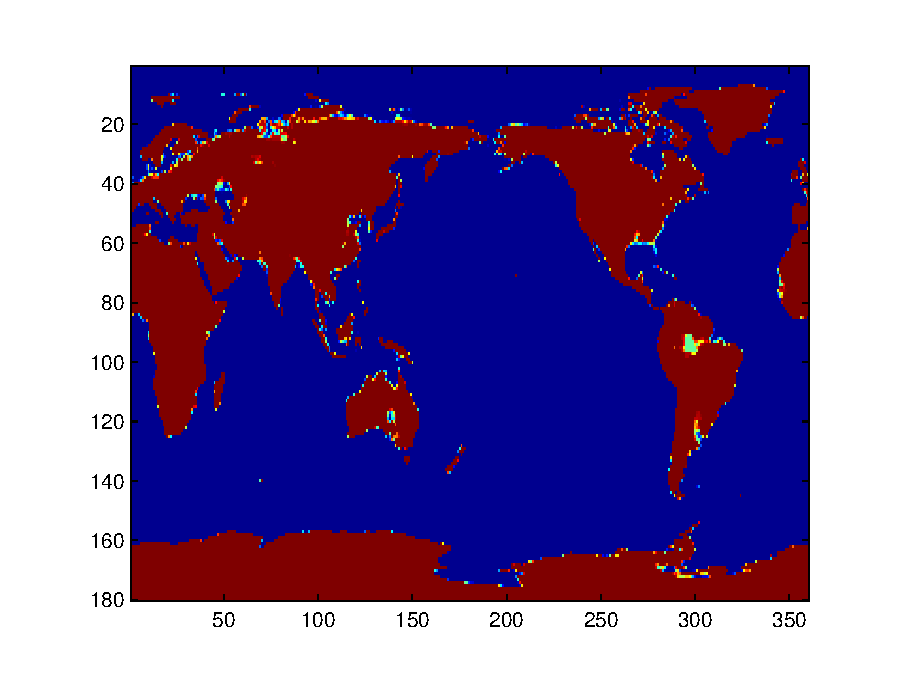
\includegraphics[width=\linewidth]{ch3-etopo.eps}
\caption{Very basic imaging (\texttt{image}) of an array (2D) of data -- here, global bathymetry.}
\label{fig:ch3-etopo}
\end{marginfigure}

This is not exactly the prettiest of images. You can distinguish ocean (blue) from land (mostly brown, but other color pixels in places). Fortunately, \textbf{MALTAB} provides a variant of this plotting function, \docenvdef{imagesc}, that calculates the color scale to exactly span the min/max values in the data. Try it (and get something like Figure \ref{fig:ch3-etopo2} hopefully).

\begin{marginfigure}[0.0in]
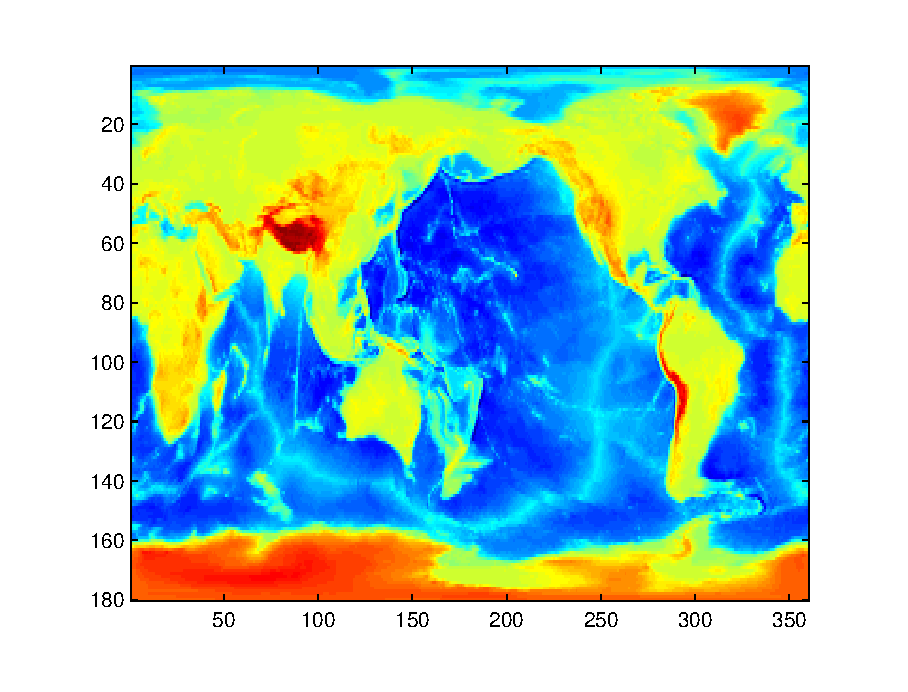
\includegraphics[width=\linewidth]{ch3-etopo2.eps}
\caption{Slightly improved very basic imaging (\texttt{imagesc}) of bathymetry data.}
\label{fig:ch3-etopo2}
\end{marginfigure}

The function \texttt{imagesc} also enables the range of data values the colo9r range corresponds to, to be set. Refer to \texttt{help} on this function and see if you can plot just the above-sealevel, i.e. land surface heights, spanning zero (sealevel) to the maximum height\sidenote{Don't forget the function \texttt{max}.}.

Which sort of in a round-about sort of way also brings us to how to set the color scale, which can be changed using the \docenv{colormap} command (see Box). Try out some different \textit{colormaps} and re-plot the global topography data.What scales work well and what do not? Which scales help pick out details of e.g. ocean floor depth variation and which help pick out simple land-sea contrasts. Think about what one might want to highlight about global topography and what color scale might be best for this purpose?

\marginnote[-0.25in]{\begin{mdframed}[backgroundcolor=gray!10, roundcorner=10pt,leftmargin=1, rightmargin=1, innerleftmargin=5, innerrightmargin=5, innertopmargin=5,innerbottommargin=5, outerlinewidth=1, linecolor=light-gray]
\docenvdef{colormap}
\\ \textbf{MATLAB} has a number of 'colormaps' built in -- color scale that determine the colors that correspond to the data. The command to change the \textit{colormap} from the default is:
\begin{docspecmargin}
>> colormap NAME
\end{docspecmargin}
where \texttt{NAME} is the name of the \textit{colormap}. You can find a list of possible \textit{colormaps} in \textbf{help} on \texttt{colormap} (in a table towards the bottom). But a brief summary is:
\begin{itemize}[noitemsep]
\setlength{\itemindent}{.2in}
\item \texttt{parula} -- the current \textbf{MATLAB} default -- chosen to provide a wide range of color and color intensity.
\item \texttt{jet} -- the old \textbf{MATLAB} default, but one which uses red and green in the same color, which should be avoided (why?).
\item \texttt{hot}, \texttt{cool} -- relatively simple color transitions but useful -- hot is something like you'll see in publication figures. 
\item \texttt{pink} -- another simple and at times useful transition and from dark (almost black) to white.
\end{itemize}
To return to the default \textit{colormap}:
\begin{docspecmargin}
>> colormap default
\end{docspecmargin}
\end{mdframed}}

%------------------------------------------------

\vspace{1mm}
\noindent\rule{4cm}{0.5pt}
\vspace{-2mm}

%------------------------------------------------

\newthought{Sticking with global Earth surface topography}, how else can we display the spatial data? For instance we might want to interpolate it, contour it, or simple get the longitude and latitude exes correct. Note that only by luck, because this particular dataset is 1 degree by 1 degree, the default axis scale in \textbf{MATLAB} when using image is approximately correct, although note that 'latitude' has been ordered in reverse and it goes from 1 to 180 rather than -90 to 90 ... We'll explicitly address this shortly.

To start with, you can simply use the \texttt{contour} function (see Box), passing only the matrix (of global topography values). Try this. Now you might want to think about flipping the matrix up-down, and/or left-right, as your plot should have come out looking like Figure \ref{fig:ch5-contour1}.

Once you have fixed the orientation of the topography map, you might play about with the color scale (\texttt{colormap}) as before. You might also try the companion to \texttt{contour} -- \texttt{contourf}. Re-orientating the matrix, switching to a different \textit{colormap}, and plotting using \texttt{contourf}, might give you something like Figure \ref{fig:ch5-contour2}.

OK, so a next refinement in plotting esp. maps and contour plots, is firstly to specify the range of the color scale, as we may not want the min-to-max range chosen by default by \textbf{MATLAB}, and the number of contours (e.g. in the topography example, they are pretty far apart and it is difficult to make out much detail). Both of these factors can be addressed simultaneously, by giving MATLAB a vector containing the value at which you want the contours drawn\sidenote{By default: MATLAB determines the minimum and maximum data values, and draws 10 equally spaced contours between these limits.}.

Taking the global topography data -- lets say you were interested only in low lying and shallow bathymetry, and wanted 20 contours intervals. Assuming a range in topographic height (relative to sealevel) of -1000 m to +1000 m, you should be able to deduce how to create the vector(?)\sidenote[][-0.0in]{ If not, it is:
\begin{docspecmargin}
>> v = [-1000:100:1000];
\end{docspecmargin}}

\marginnote[-0.0in]{\begin{mdframed}[backgroundcolor=gray!10, roundcorner=10pt,leftmargin=1, rightmargin=1, innerleftmargin=5, innerrightmargin=5, innertopmargin=5,innerbottommargin=5, outerlinewidth=1, linecolor=light-gray]
\docenvdef{contour}
There are various uses of contour. The simplest is:
\begin{docspecmargin}
contour(Z)
\end{docspecmargin}
where \texttt{Z} is a matrix. Thsi ends up similar to image except with the data contoured rather than plotted as pixels (the 'simularity' here is that the x and y axis values simple are the number of the rows and columns of the data).
\\You can specify the values at which the contours are drawn, by passing a vector (v) of these values, e.g.
\begin{docspecmargin}
contour(X,v)
\end{docspecmargin}
More involved and practical, is:
\begin{docspecmargin}
contour(X,Y,Z)
\end{docspecmargin}
where \texttt{X}, \texttt{Y}, and \texttt{Z}, are all matrices of the *same* size (there is important). \texttt{X} and \texttt{Y} contain the \textit{x} and y coordinate locations of \textit{y} data values (contained in matrix \texttt{Z}). In the example of a map -- \texttt{X} and \texttt{Y} contain the longitude and latitude values of the data values in \texttt{Z}.
\\Similarly, you can add a vector \texttt{v} containing the contours to be drawn, by:
\begin{docspecmargin}
contour(X,Y,Z,v)
\end{docspecmargin}
\end{mdframed}}

Do this and check e.g. by opening up the vector in the \textsf{Variables window}. You should see the numbers from -1000 to 1000 in intervals of 100. Why, for instance, can you not simply write:
\begin{docspec}
>> v = [-1000:1000];
\end{docspec}
??? (Or rather:\ why might this not be a good idea ... ?)

Having created a specific vector of contours to plot, try it out. OK -- so this is a little weird and maybe not so useful, but you get the point hopefully. So try plotting the following:

\begin{enumerate}[noitemsep]
\setlength{\itemindent}{.2in}
\item Just above sealevel topography, up to 10,000 m, in increments of 100 m.
\item Just the sealevel (coastline) contour ... trickier -- create a vector with a value at zero, and a value either side -- one very high and one very low. Use \texttt{contour} rather than \texttt{contourf}, although the latter produces a lovely land-sea mask!
\item Convert the data matrix of value in units of m, to ft, and plot the ocean floor (values equal to or below sealevel) in intervals of 1000 ft.
\item Finally -- try some different color scales for the above. Think about which color scales best help illustrate the data, and whether \texttt{contour} or \texttt{contourf} is clearer. Also: how many contour intervals is 'best'? You key is to make features clear, within the plot becoming cluttered or overly detailed.
\end{enumerate}

The final refinement in contour plotting we'll look at is adding labels to the contours. The command to do this is \docenv{clabel} (for 'contour label') (see Box). Now, before anything, there is a slightly complication. \texttt{clabel} needs to know details of the contours and graphics object with which to do anything with. For the purposes of this course, you don't have to worry about the details of this, but simply need to know the following:

\begin{marginfigure}[0.0in]
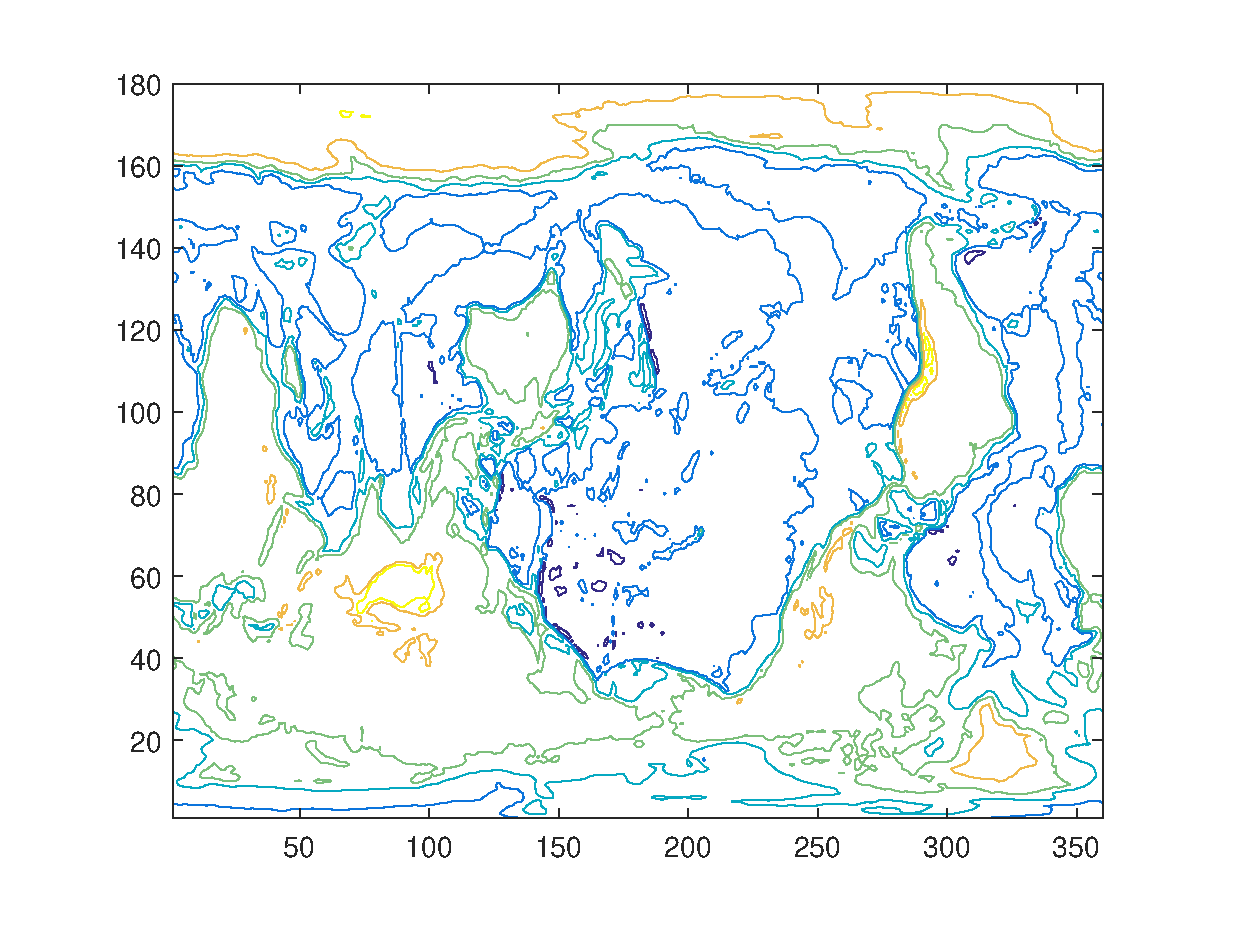
\includegraphics[width=\linewidth]{ch5-contour1.eps}
\caption{Example result of basic usage of the \texttt{contour} function.}
\label{fig:ch5-contour1}
\end{marginfigure}

\begin{enumerate}[noitemsep]
\setlength{\itemindent}{.2in}
\item When you call \texttt{contour} (or \texttt{contourf}), 2 parameters are returned, which so far you have not cared about or even noticed. We now need them. So when you call either potting function, using the syntax:
\begin{docspec}
[C,h] = contour( ... )
\end{docspec}
which saves a matrix of data to \texttt{C}, and a ID (technically: graphics object 'handle')to \texttt{h}.
\item When you call \texttt{clabel}, pass these parameters back in, e.g.
\begin{docspec}
clabel(C,h)
\end{docspec}
(in its most basic usage).
\end{enumerate}

\begin{marginfigure}[0.0in]
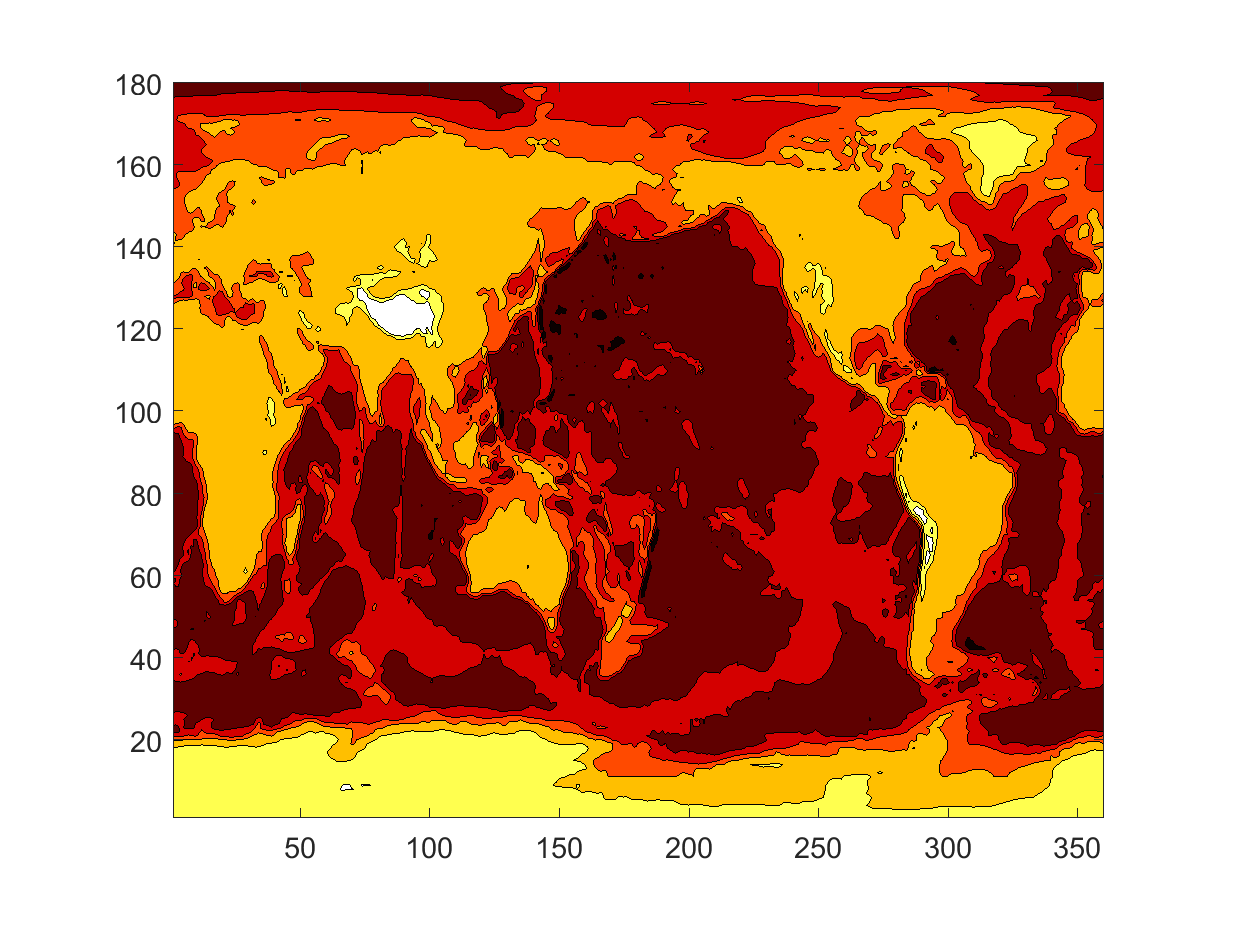
\includegraphics[width=\linewidth]{ch5-contour2.eps}
\caption{Example usage of \texttt{contourf}, with the \texttt{hot} \textit{colormap} (giving dark/brown colors as deep ocean, and light/white as high altitude).}
\label{fig:ch5-contour2}
\end{marginfigure}

\begin{marginfigure}[0.0in]
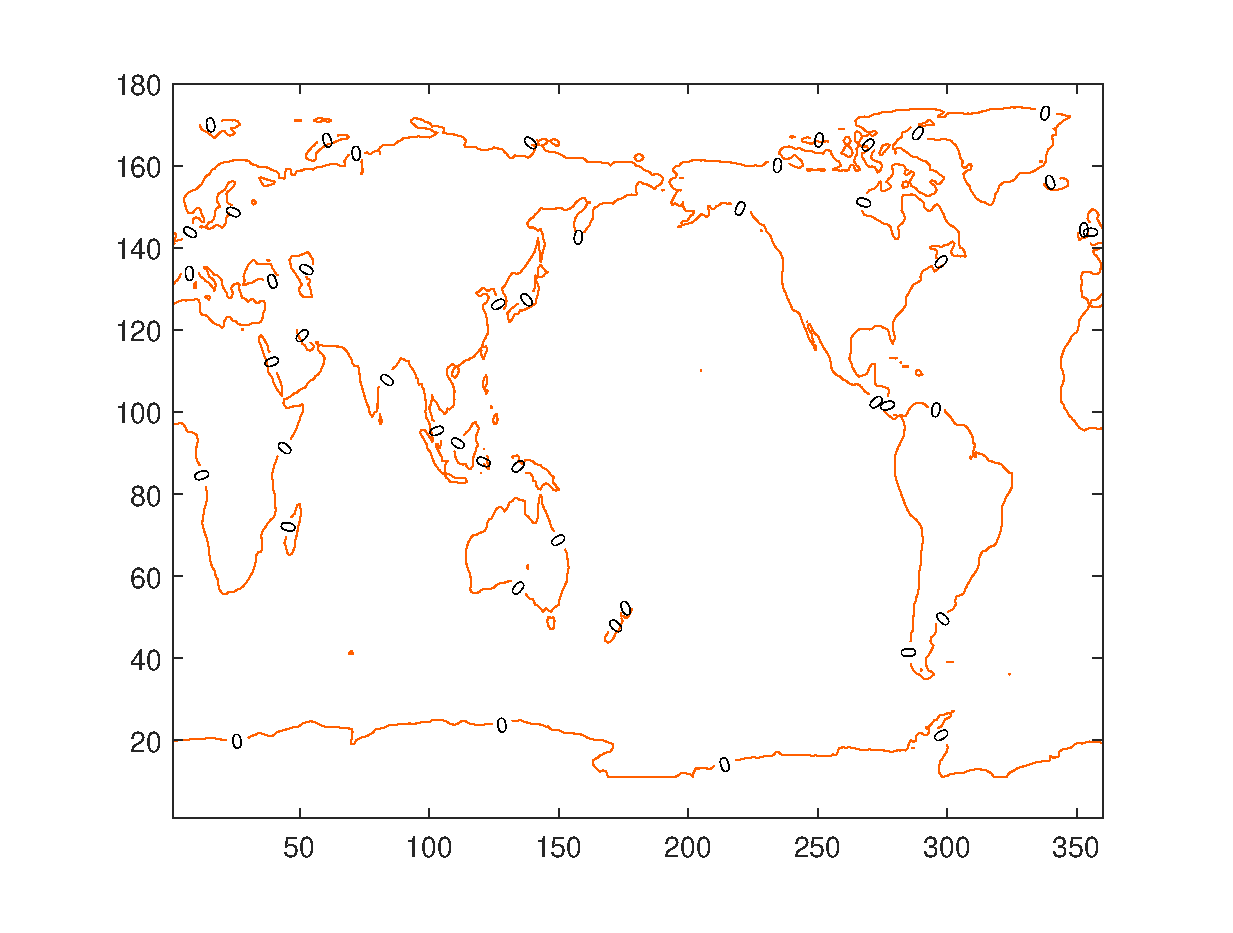
\includegraphics[width=\linewidth]{ch5-contour4.eps}
\caption{Example usage of \texttt{contour}, contouring only the zero height isoline, and providing a label.}
\label{fig:ch5-contour4}
\end{marginfigure}

If you do this, in an earlier example of plotting just the zero height contour, and now using the most basic default usage of clabel (as above), you get, for good or for bad, Figure \ref{fig:ch5-contour4}.

In the default usage of \texttt{clabel}, you'll get a label added on every contour that you plot. This ... can get kinda messy if you have lots and lots of contours plotted. You may well not need every single contour labelled, particularly if you also provide a color scale (see below). So you can also pass in a vector to tell \textbf{MATLAB} which contours to label. For example, if you have a contour interval vector:
\begin{docspec}
v = [-1000:100:1000];
\end{docspec}
maybe you onyl want labels every 500m, so you'd use a vector:
\begin{docspec}
w = [-1000:500:1000];
\end{docspec}
to specific the labelling intervals. The complete set of commands becomes:
\begin{docspec}
>> v = [-1000:100:1000];
\\ >> w = [-1000:500:1000];
\\ >> [C,h] = contour(etopo1deg,v);
\\ >> clabel(C,h,w);
\end{docspec}

\marginnote{\begin{mdframed}[backgroundcolor=gray!10, roundcorner=10pt,leftmargin=1, rightmargin=1, innerleftmargin=5, innerrightmargin=5, innertopmargin=5,innerbottommargin=5, outerlinewidth=1, linecolor=light-gray]
\docenvdef{clabel}
\begin{docspecmargin}
>> clabel(C,h)
\end{docspecmargin}
labels every contour plotted from
\begin{docspecmargin}
[C,h] = contour( ... );
\end{docspecmargin}
(or from \texttt{contourf}).
\\By prescribing and passing a vector \texttt{v} of contour intervals, you can label fewer/specific intervals rather than all of them (the default), e.g.
\begin{docspecmargin}
>> clabel(C,h,v)
\end{docspecmargin} 
\end{mdframed}}

Finally -- missing from our color-coded plots so far, is a color scale to relate values to colors (although labelling the contours works as an OK substitute). The \textbf{MATLAB} command is simple:
\begin{docspec}
>> colorbar
\end{docspec}
(and see Box for further usage). Try adding a \textit{colorbar}, and in different places in the plot. Refer to the Box to try and add a caption to it ...

\newpage

%------------------------------------------------

\vspace{1mm}
\noindent\rule{4cm}{0.5pt}
\vspace{-2mm}

%------------------------------------------------

\marginnote[-0.25in]{\begin{mdframed}[backgroundcolor=gray!10, roundcorner=10pt,leftmargin=1, rightmargin=1, innerleftmargin=5, innerrightmargin=5, innertopmargin=5,innerbottommargin=5, outerlinewidth=1, linecolor=light-gray]
\docenvdef{colorbar}
\\This almost could not be simpler:
\begin{docspecmargin}
>> colorbar
\end{docspecmargin}
plots the color scale! By default, is places it to the RH sice of the plot. If you wish for it to appear anywhere else, use the modified syntax:
\begin{docspecmargin}
>> colorbar(PLACEMENT)
\end{docspecmargin}
where PLACEMENT is one of: \texttt{'northoutside'}, \texttt{'southoutside'}, \texttt{'eastoutside'}, \texttt{'westoutside'}. Note that these are strings and so need to be in quotation marks. (More options are summarized in a table in \textbf{help}.)
\\Finally, you can also add a label to the \textit{colorbar}, but only if you get hold of its ID ('graphics handle') when you call \texttt{colorbar}, e.g.
\begin{docspecmargin}
>> h = colorbar
\end{docspecmargin}
will save the graphics handle in variable \texttt{h}, which you can then muck about with via:
\begin{docspecmargin}
c.Label.String = 'The units of my lovely colorbar';
\end{docspecmargin}
(Don't fight this -- use this syntax to set a label for the \textit{colorbar} -- don't worry about  what it means. \textbf{MATLAB} keeps rather annoyingly changing the way it does this anyway :()
\end{mdframed}}

\newthought{In this next Example}, we'll address the issue with missing/incorrect lon/lat axis labels on the plots.

Each data point in the \texttt{etopo1deg} matrix should have one longitude value (\textit{x}-axis) and one latitude (\textit{y}-axis) value associated with it. It should hopefully be intuitive to you now ... that what we need is a pair of matrices, of exactly the same size as the \texttt{etopo1deg} data matrix -- one holding longitude values and one latitude values. There are various ways of creating the required matrices 'by hand' (or involving writing a program including a \textit{loop}). All of them are tedious. There is a \textbf{MATLAB} function to help. But it is not entirely intuitive\sidenote{\textbf{\textcolor{red}{DON'T\ PANIC!}}} ... \docenv{meshgrid}.

Spend a few minutes reading about it in \texttt{help}. In particular, look at the examples given to help you translate the \textbf{MATLAB}-speak gobbledegook of the function description. You should be able to glean from all this that this function allows us to create two \(a\times b\) arrays; one with the columns all having the same values, and one with the rows all having the same values (exactly what we need for defining the (lon,lat) of all the global data points). If not, and probably not -- see Box. And then lets do a simple example (adapted from \textbf{help}):
\begin{docspec}
>> [X,Y] = meshgrid(1:3,10:14)
\\X =
\\ \ \ \ \ 1     2     3
\\ \ \ \ \ 1     2     3
\\ \ \ \ \ 1     2     3
\\ \ \ \ \ 1     2     3
\\ \ \ \ \ 1     2     3
\\Y =
\\ \ \ \ \ 10    10    10
\\ \ \ \ \ 11    11    11
\\ \ \ \ \ 12    12    12
\\ \ \ \ \ 13    13    13
\\ \ \ \ \ 14    14    14
\end{docspec}
Here, we are taking 2 vectors -- \texttt{[1:3]} and \texttt{[10:14]}, and asking \textbf{MATLAB} (very nicely) to create 2 matrixes, one in which \texttt{[1:3]} is replicated down, until it has the same number of rows as the length of \texttt{[10:14]}, and one in which \texttt{[10:14]} is replicated across until it has the same number of columns as the length of \texttt{[1:3]}. (Try it.)

It'll become apparent *why* bother shortly. Honest.

\marginnote[-2.50in]{\begin{mdframed}[backgroundcolor=gray!10, roundcorner=10pt,leftmargin=1, rightmargin=1, innerleftmargin=5, innerrightmargin=5, innertopmargin=5,innerbottommargin=5, outerlinewidth=1, linecolor=light-gray]
\docenvdef{meshgrid}
\\The unholy syntax is:
\begin{docspecmargin}
[X,Y] = meshgrid(xv,yv)
\end{docspecmargin}
Pause, and take a deep breath. On the left -- the results of \texttt{meshgrid} are being returned to 2 matrixes, \texttt{X} and \texttt{Y}. These are going to be our matrixes of the longitude and latitude values (in the particular example in the text). So far so good(?)
\\On the right, passed into the function \texttt{meshgrid}, are two vectors -- \texttt{xv} and \texttt{yv}. Pause again.
\\What \textbf{MATLAB} is going to do, is to take the (row) vector \texttt{xv}, and it is going to replicate it down so that there are as many rows as in the vector \texttt{yv}. This becomes the returned output matrix \texttt{X}. \textbf{MATLAB} then takes the column vector \texttt{yv}, and replicates it across so that there are as many columns as in the vector \texttt{xv}. This becomes the returned output matrix \texttt{Y}.
\end{mdframed}}

In our Example -- start by noting that the topography data is on a regular 1 degree grid starting at 0\degree\ longitude. Latitude starts (at the bottom) at -90\degree\ and goes up to +90\degree\ ). We need a matrix containing all the longitude values from 0\degree\ to 359\degree\, and latitude from -90\degree\ to 89\degree\ .\sidenote{There is a slight complication with this, which we'll get to shortly, but note that the data array is 360 elements (\textit{x}-direction) by 180 elements (\textit{y}-direction).} These matrices need to be the same size as the data matrix.

Maybe just do it and then understand what has happened after. Create the longitude and latitude grids by:
\begin{docspec}
>> [lon lat] = meshgrid([0:359],[-90:89]);
\end{docspec}

View (in the \textsf{Variables window}) the \texttt{lon} matrix first. Scan through it. Hopefully ... you'll note that it is 360 columns across, and in each column has the same value -- the longitude. The matrix is 180 rows 'high', so that there is a longitude value for each latitude. Similarly, view \texttt{lat}. This also should make a little sense if you pause and think about it, with the one exception that the South Pole latitude is at the 'top' of the matrix -- don't worry about this for now ... 

The only way to fully make sense of things now, is to use it. Remember that use of \texttt{contour} (and \texttt{contourf}) can take matrices of \textit{x} and \textit{y} (here: longitude and latitude) values that correspond to the data entries in the data matrix (\texttt{etopo1deg}). Re-load the topography data in case you have flipped it about in all sorts of odd ways, and then do:
\begin{docspec}
>> [lon lat] = meshgrid([0:359],[-90:89]);
\\ >> contour(lon,lat,etopo1deg);
\end{docspec}
Almost! Note that the \textit{x} and \textit{y} axis labelling is 'correct' and particularly the \textit{y}-axis, where latitude goes from -90 to 90 (although by default \textbf{MATLAB} labels in intervals of 20 starting at -80 it seems). But it also turns out that we do need to flip the data op-side-down. We can actually do this in the same line as we plot:
\begin{docspec}
>> contour(lon,lat,flipud(etopo1deg));
\end{docspec}
Phew! (Figure Figure \ref{fig:ch5-contour5}.)

\begin{marginfigure}[0.0in]
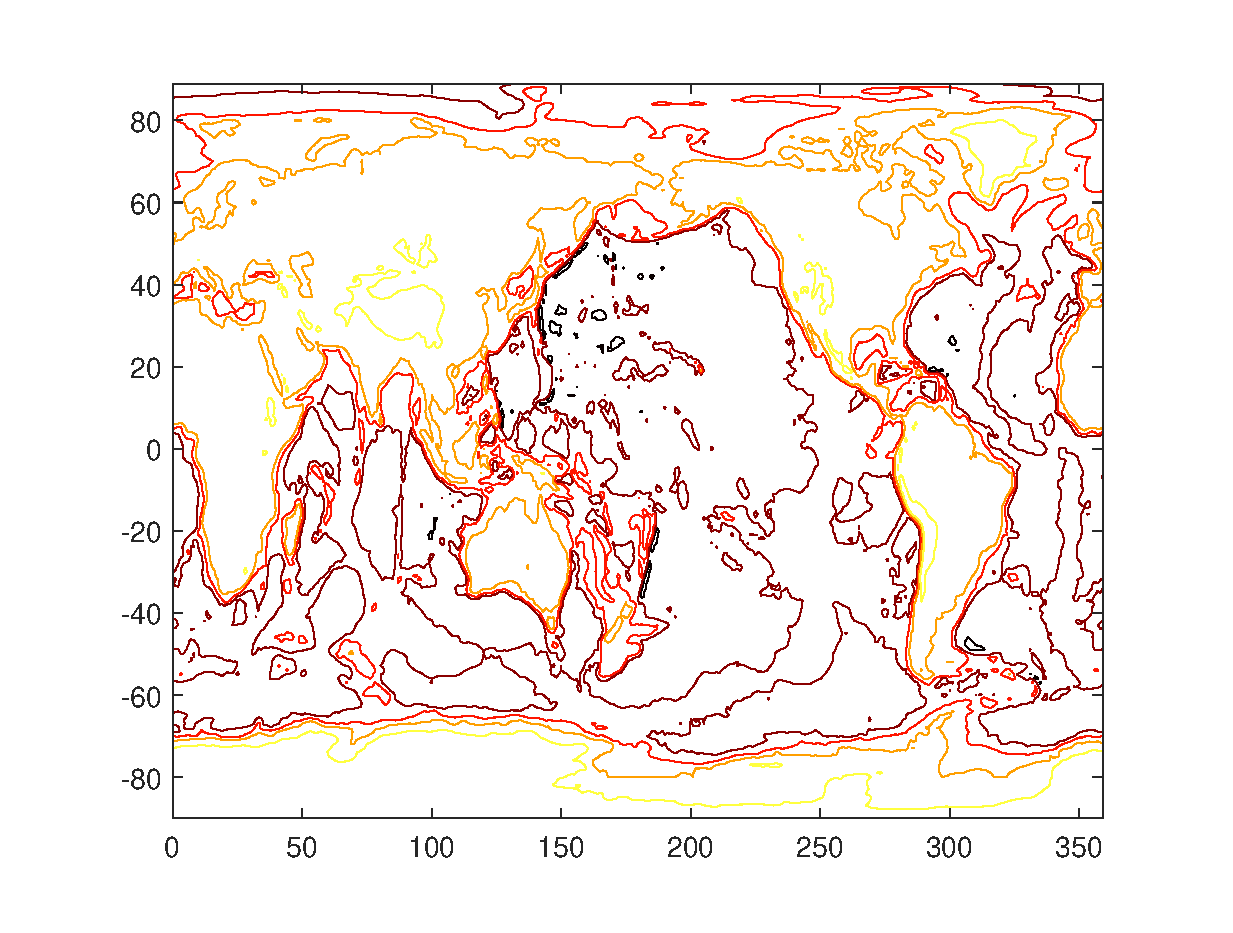
\includegraphics[width=\linewidth]{ch5-contour5.eps}
\caption{Usage of \texttt{contour} but with lon/lat values created by \texttt{meshgrid} function and passed in (and with the \texttt{hot} \textit{colormap} (giving dark/brown colors as deep ocean, and light/white as high altitude).}
\label{fig:ch5-contour5}
\end{marginfigure}

The final complication is that the data points in the gridded dataset (matrix \texttt{etopo1deg}), technically correspond to the mid-points of a 1 degree grid, not the corners. So if we were going to try and be formally correct\sidenote{Don't worry about this for now -- grids will be covered more in subsequence chapters surrounding numerical (environmental) models.}, our vectors that we'd pass into \texttt{meshgrid}, would be:
\begin{docspec}
>> xv = [0.5:359.5];
\\ >> yv = [-89.5:89.5];
\end{docspec}

%------------------------------------------------

\vspace{1mm}
\noindent\rule{4cm}{0.5pt}
\vspace{-2mm}

%------------------------------------------------

\newthought{OK -- another Example} on this. Previously, you downloaded and plotted monthly global distributions of surface air temperature. You plotted these simply using \texttt{pcolor} (or \texttt{image}) and the results were ... variable. Certainly not publication-quality graphics and missing appropriate longitude and latitude axes for the plots.

Make a copy of your original \textit{script} (\textsf{m-file}) in which you created the animation, and give it a new name. Edit your program, and in place of \texttt{pcolor}, use \texttt{contour} or \texttt{contourf} (your choice!). Pass in just the data matrix (of monthly temperature) when calling the \texttt{contour}(\texttt{f}) function and don't yet worry about the lon/lat values. Get this working (i.e. debug it if not). You should end up with a contoured animation (rather than a bit-map animation).

The problem with the axis labelling should be much more apparent (than compared to the topography data, which was on a handy 1 degree grid already). So you need to make a matrix of longitude values, and one of latitude. using \texttt{meshgrid}. The grid is a little awkward:
\begin{enumerate}[noitemsep]
\setlength{\itemindent}{.2in}
\item The longitude grid runs from 0\degree E (column \#1) with an increment of 1.875\degree ; i.e., 0.000\degree E, 1.875\degree E, 3.750\degree E, ... up to 358.125\degree E (column \#192).
\item Latitude runs from 88.54196\degree S (-88.54196\degree N) at row \#1, to 88.54196\degree N (row \#94) with an increment of about 1.904.
\end{enumerate}
so I'll give you the answer up-front:
\begin{docspec}
>> lonv = [(1.875/2):1.875:360-(1.875/2)];
\\>> latv = [-90+(1.904/2):1.904:90-(1.904/2)];
\\>> [lon lat] = meshgrid(lonv,latv);
\end{docspec}
Now use the longitude and latitude values matrices, in conjunction with \texttt{contour}(\texttt{f}), to plot the global temperature distributions 'properly'. Try plotting just one plot first, before looping through all 12 months. 

At this point (before creating an animation), you might also explore some of the plotting refinements we saw earlier. For example, as per Figure \ref{fig:ch5-contour6}. 
Firstly -- get the units of the temperature data array into units of \degree C (or \degree  F if you are into that sort of thing) rather than \degree K. Either: assign the \texttt{temp} array data to a new array and make the appropriate conversion from \degree K (all within the loop), or you can do this subtraction on the line that you actually plot the data (i.e., within the \texttt{contour}/\texttt{contourf} function), for example:
\begin{docspec}
contourf(lon(:,:),lat(:,:),temp(:,:,month)-273.15);
\end{docspec}
\noindent would convert to \degree C as it plotted the data.

You can also get the plotting temperature limits and contouring consistent between months and with greater resolution by adding the following line (before the loop starts):
\begin{docspec}
v=[-40:2:40];
\end{docspec}
\noindent and then to the \texttt{contour(...)} (or \texttt{contourf(...)}) function, add \texttt{,v} to the end of the list of passed parameters. This particular choice for the vector \texttt{v} tells \textbf{MATLAB} to do the contouring from -40 to 40 (\degree C), and at a contour interval of 2 (\degree C).. Play around with the min and max limits of the range, and also with the contour interval to see what gives the clearest and least cluttered plot. For instance, maybe you don't want the low temperatures to go 'off' the scale (the white color in the filled contour plot).

\begin{marginfigure}[0.0in]
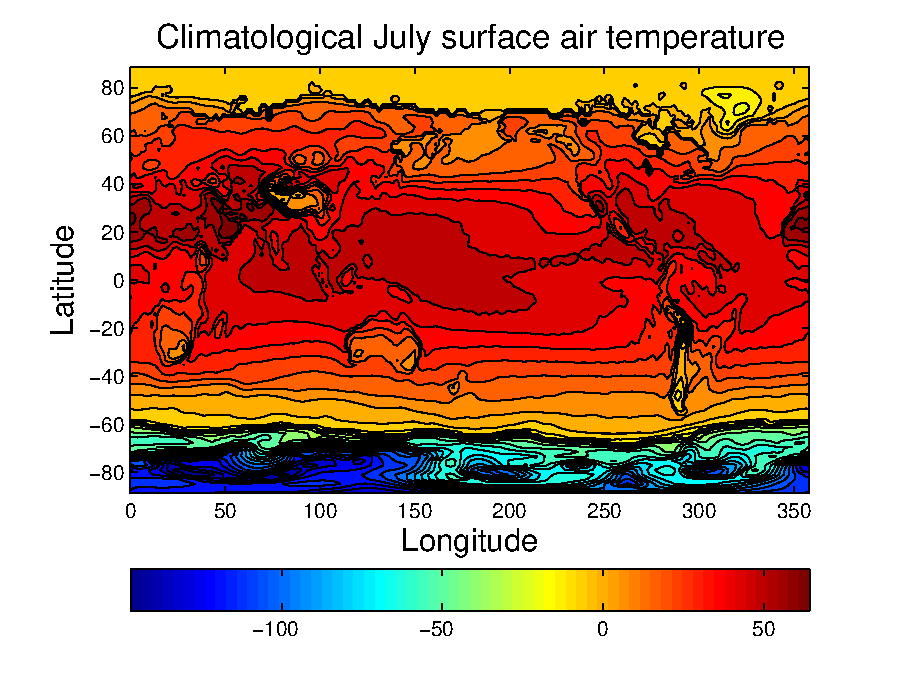
\includegraphics[width=\linewidth]{ch5-contour6.eps}
\caption{Example contour plot including \texttt{meshgrid}-generated lon/lat values. Result of \texttt{contourf(lon,lat,temp7,30)}, where the data file was \texttt{temp7.tsv}, with some embellishments.}
\label{fig:ch5-contour6}
\end{marginfigure}

%------------------------------------------------

\vspace{1mm}
\noindent\rule{4cm}{0.5pt}
\vspace{2mm}

\noindent Lastly -- for any (or all) of the Examples above, you could add the continental outline to the plot. Remember, to use \texttt{hold on} in order to overlay the continental outline on top of the contour map without replacing it in the \textsf{Figure window}.

It should be obvious that plotting the continental outline might be something you want to us more than once. Sections of code that might get used multiple times are commonly placed in a file (or special section of the file) of their own and \textit{called} from the main program that needs it. For example, you could place the entire continental outline plotting code, including loading in the data, in an \textsf{m-file} and make it a function -- in this case, taking no parameters as input, and return no output.\sidenote{Make sure that you do not open a figure window with the \texttt{figure} command with the function, or you will not get a continental output overlay on your plot, but rather a sperate \textsf{Figure window} with just the continental outline on.} In the example of the looped animation, in the sequence of code (within the loop), you will need to \textit{call} your continental outline plotting function just after you have plotted the contour (or bitmap) plotting function.

%------------------------------------------------

\subsection{Using the MATLAB Mapping toolbox}

You can do some nice spatial plotting with this data using the \textbf{MATLAB} \textsf{Mapping Toolbox}. This should be available as part of the \textbf{MATLAB} installation in the Lab (and also if you have downloaded and installed an academic version on a personal laptop). Refer to the on-line documentation for the \textsf{Mapping Toolbox} to get you started. The key function appears to be \docenvdef{geoshow}. Try plotting the region encompassing the 'quake data, with a coastal outline (of land masses), and the 'quake data overlain. Explore different map projections. Remember to always ensure appropriate labelling of plots.

%------------------------------------------------

\newpage

%------------------------------------------------

\section{Further data processing}

This section contains a selection of further simple techniques for doing useful stuff with data, as well as for better graphing.

%------------------------------------------------

\newpage

%------------------------------------------------

\subsection{\texttt{find}!}

So -- a single \textbf{MATLAB} function gets its own sub-section, all to itself. Either it's really powerful and useful, or I am running out of ideas for the text\sidenote{It is really powerful and useful.}.

\marginnote{\begin{mdframed}[backgroundcolor=gray!10, roundcorner=10pt,leftmargin=1, rightmargin=1, innerleftmargin=5, innerrightmargin=5, innertopmargin=5,innerbottommargin=5, outerlinewidth=1, linecolor=light-gray]
\docenvdef{find}
\\\textbf{MATLAB} defines find, with a basic syntax of:
\begin{docspecmargin}
k = find(X)
\end{docspecmargin}
as '\textit{return[ing] a vector containing the linear indices of each nonzero element in array X}'.
\\That means ... nothing to me. This is going to have to be a job for some Examples ... (in order to see what \docenv{find} is all about).
\\ Actually, \texttt{find} returns the indices of the non-zero elements in the array and if the array is a vector, what is does is simple. For a matrix, \texttt{MATLAB} counts the elements sequentially, starting at the 1st row and 1st column, and working down the first column, rather than provide the (row,column) for indexing format you are used to. Hence where the '\textit{linear indices}' bit comes in.
\\ Furthermore, 'non-zero' indices is really just code-word for 'true'. So you are asking where the true values occur in \texttt{X}. If \texttt{X} is the answer to a \textit{logical} or \textit{relational} operation, then find tells you the indices of the elements that are true.
\\ For example, \texttt{3 > [5 3 1]} equates to \texttt{[0 0 1]}, i.e. only the first element in the vector \texttt{[5 3 1]} is less than \texttt{3}. Hence:
\begin{docspecmargin}
find(3 > [5 3 1])
\end{docspecmargin}
first evaluates the relational operation and generates a vector of true and false values, and then \texttt{find} tells you the index (or indices) where the true values occur (here, \texttt{ans = 3}).
\end{mdframed}}

\docenv{find} ... finds where-ever in an \textit{array}, a specific condition is met. If the specific condition occurs once, a single \textit{array} location is returned. The specific condition could occur multiple times, in which case \texttt{find} will report back multiple positions in the \textit{array}.

What do I mean by a 'specific condition'? Basically -- exactly as per in the \texttt{if ...} construction -- a \textit{conditional} statement being evaluated to \textit{true}.

OK -- some initial Examples.

Say that you have a vector of numbers, e.g.:
\begin{docspec}
A = [3 7 5 1 9 7 4 2];
\end{docspec}
and you want to find the maximum value in the vector -- easy.\sidenote{I hope so ... check back earlier (or slightly later) in the course on \texttt{max}.}

But ... you want to find *where* in the vector the maximum value occurs. Why might you want to do this? Rarely do you have a single vector of data on its own -- generally it is always linked to at least one other vector (often time or length in scientific examples). Trivially, our second vector might be:
\begin{docspec}
B = [0:7];
\end{docspec}
and is time in units of \(ms\)\sidenote[][0.25in]{Why? Why not.}. The question then becomes: at what time did the maximum value occur? Obviously, this is easy by eye with just 8 numbers, but if you had 1000s ...

We can start by determining the maximum value (in the data array, \texttt{A}).
\begin{docspec}
c = max(A);
\end{docspec}

Now, we use \docenv{find} to evaluate where in  array \texttt{A} (here: a vector) the element with a value of \texttt{max(A)} (equal to \texttt{c}) occurs. The following should accomplish this:

\begin{docspec}
find(A(:)==c);
\end{docspec}

Here, what we are saying is: take all of the elements in \texttt{A} and \uline{find} where an element occurs that is equal to \texttt{c} (the maximum value, which we already determined). Try it, and \textbf{MATLAB} should return \texttt{5} -- the 5th element in the vector.

Finally, if we assign the result of \texttt{find} to \texttt{d}, remembering that \texttt{find} return an array index (or indices), we can then use \texttt{d} to determine the time at which the value of \texttt{9} occurred, i.e. \texttt{B(d)} which evaluates to \texttt{4} (ms):

In this example, \docenv{find} returned just a single element, but if we instead had:
\begin{docspec}
A = [3 9 5 1 9 7 4 2];
\end{docspec}
The maximum value is still the same (\texttt{9}) but now ...
\begin{docspec}
>> find(A(:)==c)\\
ans =
\\ \ \ \ \ 2
\\ \ \ \ \ 5
\end{docspec}

What has happened is that \docenv{find} has determined that there are 2 elements in vector \texttt{A} that satisfy the condition of being equal to \texttt{c} (\texttt{9}) and that these lie at positions (index) \texttt{2} and \texttt{5}. The result \textit{vector}, if you assigned it to the variable \texttt{d} again, can be used just as before to access the corresponding times in vector \texttt{B};
\begin{docspec}
>> d = find(A(:)==c);\\
>> B(d)
\\ans =
\\ \ \ \ \     1     4
\end{docspec}
i.e. that the times at which the values of \texttt{9} occur are \texttt{1} and \texttt{4} (\(ms\)).

Any of the \textit{relational operators} (that evaluate to \textit{true} or \textit{false}) can be used. In fact -- looking at it this way leads us to maybe understand the \textbf{MATLAB} \textbf{help} text, because \textit{true} and \textit{false} are equivalent to \texttt{1} and \texttt{0}, and \texttt{find} is defined as a function that returns the indices of the non-zero elements in a \textit{vector}. By writing \texttt{A(:)==c} we are in effect creating a vector of \texttt{1}s and \texttt{0}s depending on whether the equality is \textit{true} or not for each element. You can pick apart what is going on and see that this is the case, by typing:
\begin{docspec}
>> A(:)==c
\\ans =
\\ \ \ \ \ 0
\\ \ \ \ \ 1
\\ \ \ \ \ 0
\\ \ \ \ \ 0
\\ \ \ \ \ 1
\\ \ \ \ \ 0
\\ \ \ \ \ 0
\\ \ \ \ \ 0
\end{docspec}
(the statement being \textit{true} at positions (index) \texttt{2} and \texttt{5}, which is exactly what \texttt{find} told you).

For instance, we could ask \texttt{find} to tell us which elements of A have a value greater than 5:
\begin{docspec}
>> find(A(:)>5)
\\ ans =
\\ \ \ \ \ 2
\\ \ \ \ \ 5
\\ \ \ \ \ 6
\end{docspec}
(Inspect the contents of vector \texttt{A} and satisfy yourself that this is the case.)

We can also use \texttt{find} to filter data. Perhaps you do not want values over 5 in the dataset. Perhaps this is above the maximum reliable range of the instrument that generated them. Having obtained a vector of locations of these values, e.g.
\begin{docspec}
d = find(A(:)>5);
\end{docspec}
we can plug this vector back into \texttt{A} and assign arrays of zero size to these locations -- effectively, deleting the locations in the array, i.e.
\begin{docspec}
A(d) = [];
\end{docspec}
They it, and note that the size\sidenote{Use the command \texttt{length} or view in the \textsf{Workspace Window}.} of \texttt{A} has shrunk to \texttt{5} -- all the other elements remain, and in order, but the elements with a value greater than 5 have gone. You could apply an identical deletion (filtering) to the time array (\texttt{B(d) = []}).

Play about with some other relational operators and criteria, and make up some vectors of your own until you are comfortable with using \texttt{find}. 
%------------------------------------------------

\vspace{1mm}
\noindent\rule{4cm}{0.5pt}
\vspace{-2mm}

%------------------------------------------------

\newthought{For an Example of data-filtering} -- dig out the paleo-proxy (\texttt{paleo\_CO2\_data.txt}) atmospheric CO\(_{2}\) data you downloaded earlier. One further way of plotting with \texttt{scatter} is to scale the point size by a data value. We could do with by:
\begin{docspec}
SCATTER(data(:,1),data(:,2),data(:,2))
\end{docspec}
... except ... it turns out that there are atmospheric CO\(_{2}\) values of zero or less and you cannot have an area (size) value of zero or less ...

\marginnote{\begin{mdframed}[backgroundcolor=gray!10, roundcorner=10pt,leftmargin=1, rightmargin=1, innerleftmargin=5, innerrightmargin=5, innertopmargin=5,innerbottommargin=5, outerlinewidth=1, linecolor=light-gray]
\docenvdef{NaN}
\\... is \textbf{Not-a-Number} and is a representation for something that cannot be represented as a number, although if you try and divide something by zero \textbf{MATLAB} reports \texttt{Inf} rather than a \texttt{NaN}.
\\ \texttt{NaN} can also be used as a function to generate arrays of \texttt{NaN}s. The most common/usage in this context is:
\begin{docspecmargin}
N = NaN(sz1,...,szN)
\end{docspecmargin}
which will (according to \textbf{help}) "generate a a sz1-by-...-by-szN array of NaN values where sz1,...,szN indicates the size of each dimension. For example, \texttt{NaN(3,4)} returns a 3-by-4 array of NaN values."
\end{mdframed}}

This leads us to a new use for \docenv{find} and some basic data filtering. The simplest thing you could do to ensure that no zero value appear anywhere, would be to add a very small number to all the values. This would defeat the 'no zero' parameter restriction, but would not help if there were negative values and you have now slightly modified and distorted the data which is not very scientific. Substituting a \docenv{NaN} for problem values is a useful trick, as \textbf{MATLAB} will simply ignore and not attempt to plot such values.

So first, lets replace any zero in the CO\(_{2}\) column of the data with a \texttt{NaN}. The compact version of the command you need is:
\begin{docspec}
data(find(data(:,2)==0),2)=NaN;
\end{docspec}
But as ever -- perhaps break this down into separate steps and use additional arrays to store the results of intermediate steps, if it makes it easier to understand, e.g.
\begin{docspec}
list\_of\_zero\_locations = find(data(:,2)==0);
\\data(list\_of\_zero\_locations,2) = NaN;
\end{docspec}
What this is saying is: first find all the locations (row indices) in the 2nd column of \texttt{data} for which the value is equivalent (\texttt{==}) to zero. Replace the CO\(_{2}\) value in all these rows (which is originally zero) to a \texttt{NaN} (technically speaking: assign a value of \texttt{NaN} to these locations). You have now filtered out zeros, and replaced the offending values with a \texttt{NaN} and when \textbf{MATLAB} encounters \textit{NaNs} in plotting -- it ignores them and omits that row of data from the plot.
 
Alternatively, we could have simply deleted the entire row containing each offending zero.  Breaking it down, this is similar to before in that you start by identifying the row numbers of were zeros appear in the 2nd column, but now we set the entire row to be 'empty', represented by \texttt{[]}:
\begin{docspec}
list\_of\_zero\_locations = find(data(:,2)==0);
\\data(list\_of\_zero\_locations,:) = [];
\end{docspec}
If you check the \textsf{Workspace window}\sidenote{Or: \\\texttt{>> size(data)}}, you should notice that the size of the array data has been reduced (by 4 rows, which was the number of times a zero appeared in the 2nd column).

We are almost there with this example except it turns out that there is a CO\(_{2}\) proxy data value less than zero(!!!) We can filter this out, just as for zeros. I'll leave this as an exercise for you\sidenote{But you might e.g. use \texttt{<=}.} ... The plot should end up looking like Figure \ref{fig:plot-CO2scatter3}. As another lesson-ette, given that the circles are insanely large ... try plotting this with proportionally smaller circles\sidenote{HINT: you are going to want to apply a scaling factor to the vector you passed as the point size data.}.

\begin{marginfigure}[0.0in]
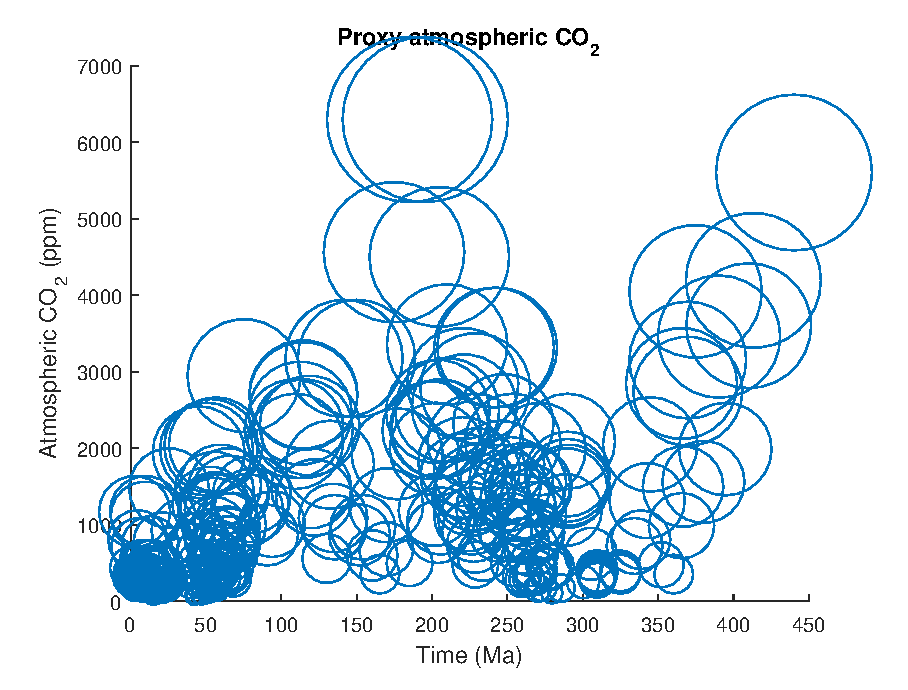
\includegraphics[width=\linewidth]{plot-CO2scatter3.eps}
\caption{Proxy reconstructed past variability in atmospheric CO2 (scatter plot).}
\label{fig:plot-CO2scatter3}
\end{marginfigure} 

Conversely, having inserted \texttt{NaN}s into an array, or having ended up with \texttt{NaN}s in an array for other reasons, you can also search for (\texttt{find}) the \texttt{NaN}s.
The first thing to note in looking for NaNs, is you cannot test for a NaN with a simple equality operator:

\begin{docspec}
>> a=NaN;\\
>> a==NaN\\
ans =\\
\ \ \ 0
\end{docspec}

\noindent which ... is odd. Having assigned a \texttt{NaN} to variable a, \textbf{MATLAB} apparently is telling you have a is not equivalent to \texttt{NaN}.
Really unhelpful.
In fairness, a does not have a value and is Not A Number and hence \textbf{MATLAB} cannot determine whether or not it is equal to another Not A Number.
 Better would have been for \textbf{MATLAB} to give you an error ... still, it is what it is.

\marginnote{\begin{mdframed}[backgroundcolor=gray!10, roundcorner=10pt,leftmargin=1, rightmargin=1, innerleftmargin=5, innerrightmargin=5, innertopmargin=5,innerbottommargin=5, outerlinewidth=1, linecolor=light-gray]
\docenvdef{isnan}
\\'\textit{\texttt{isnan(A)} returns an array the same size as \texttt{A} containing logical \texttt{1} (true) where the elements of \texttt{A} are \texttt{NaN}s and logical \texttt{0} (false) where they are not.}'
\\Meaning that you can pass any dimension of array (e.g. vector or matrix or 3D), not just a scalar (a single value or \(1\times1\) matrix). 
\end{mdframed}}

To try and make amends, \textbf{MATLAB} provides a \textit{function} to determine whether or not something is Not A Number -- \docenvdef{isnana}. This returns \textit{true} (\texttt{1}) is the passed variable is Not A Number, and \textit{false} (\texttt{0}) if not, e.g.

\begin{docspec}
>> isnan(a)\\
ans =\\
\ \ \ 1
\end{docspec}

\noindent whereas:

\begin{docspec}
>> isnan(99)\\
ans =\\
\ \ \ 0
\end{docspec}

\noindent because \texttt{99} is a number (integer) and not a Not A Number.

\vspace{1mm}
\noindent\rule{4cm}{0.5pt}
\vspace{2mm}

\noindent In the CO\(_{2}\) data, there are min and max uncertainty limit values. One could color-code the points in a scatter-plot to represent either the min or the max (perhaps try this first), but one on its own is not necessarily much use. One could color-code by the difference, but this is a function of the absolute value and one would expect large uncertainty bars if the mean (central) estimate was high, and lower if it were low. Perhaps we need the \textit{relative} range in uncertainty? Can you do this? i.e., \texttt{scatter}-plot the mean CO\(_{2}\) estimate (as a function of time), but color-coding for the range in uncertainty as a proportion of the value?

It turns out this is not entirely trivial because as you have seen, the data is not as well behaved as you might have hoped. In fact, it is just like real data you might encounter all the time! Before you do anything -- break down into small steps what you need to do with the data, as this will inform what (if any) additional processing you might have to carry out on the data. It should be obvious, that to create a CO\(_{2}\) difference, \textit{relative} to the mean, you are going to have to divide by the mean value (the values in column \#2 of the array).  So first off -- if any of the mean values are zero, it is all going to go pear-shaped (dividing by zero ...). Actually, equally unhelpful, or at least, lacking in any meaning, may be negative values. If you inspect the data (in the \textsf{Variable window}), there are both zeros and negative values for mean CO\(_{2}\) proxy estimates. We need to get rid of these. Follow the steps as before (i.e. identifying zero of negative values and either removing the corresponding rows in the array, or setting the values to a \texttt{NaN}). You may also have to process the min and max values should they turn out to be the same. Likely, you are going to have to delete all the rows in which: (1) column \#2 values are zero or below, and (2) column \#3 and \#4 values are equal (you could also try the \texttt{NaN} substitution and see if it works out).
(If you need a slight hint ... one possible answer is here\sidenote[][-1.375in]{
In this possible solution -- all rows in the array \texttt{data}, with mean CO2 values less than or equal to zero, are deleted. Also, all rows for which the max and min values are the same, are also deleted.
\texttt{\scriptsize{
\\>> data=load('paleo\_CO2\_data.txt',\\...'-ascii');
\\>> data(find(data(:,2)<=0),:)=[];
\\>> data(find(data(:,3)==data(:,4)),:)\\...=[];
\\>> scatter(data(:,1),data(:,2),40, \\...100*(data(:,4)-data(:,3))./data(:,2), \\...'filled');
\\>> xlabel('Time (Ma)')
\\>> ylabel('Atmospheric CO\_2 (ppm)')
\\>> title('Proxy atmospheric CO\_2')
}}}
, but try and work it out for yourself.)

All that is missing now, is any indication of what the color scale actually means in terms of values (and of what). \textbf{MATLAB} will add a colorbar to a plot with the command ... \docenvdef{colorbar}. Although the color scale gets automatically plotted with labels for the values, looking at the plot, we still don't know what the values are of (e.g. units). We can label the colorbar, but \textbf{MATLAB} needs to know what we are labelling. Each graphic object is assigned a unique ID when you create them and which normally you know nothing about. We can create a variable to store the ID, and then pass this ID to \textbf{MATLAB} to tell it to create a title for the colorbar. To cut a long story short:
\begin{docspec}
colorbar\_id=colorbar;
\\title(colorbar\_id,'Relative error (\%)';
\end{docspec}

It should end up looking something like Figure \ref{fig:plot-CO2scatter4} in which you can see the high relative uncertainty (bight colors) prevail at low CO\(_{2}\) values and 'deeper time' (ca. 200-300 Ma). The colorbar title (label) is maybe not ideal, nicer would be one aligned vertically rather than horizontally. We'll worry about that sort of refinement another time.

\begin{marginfigure}[-3.75in]
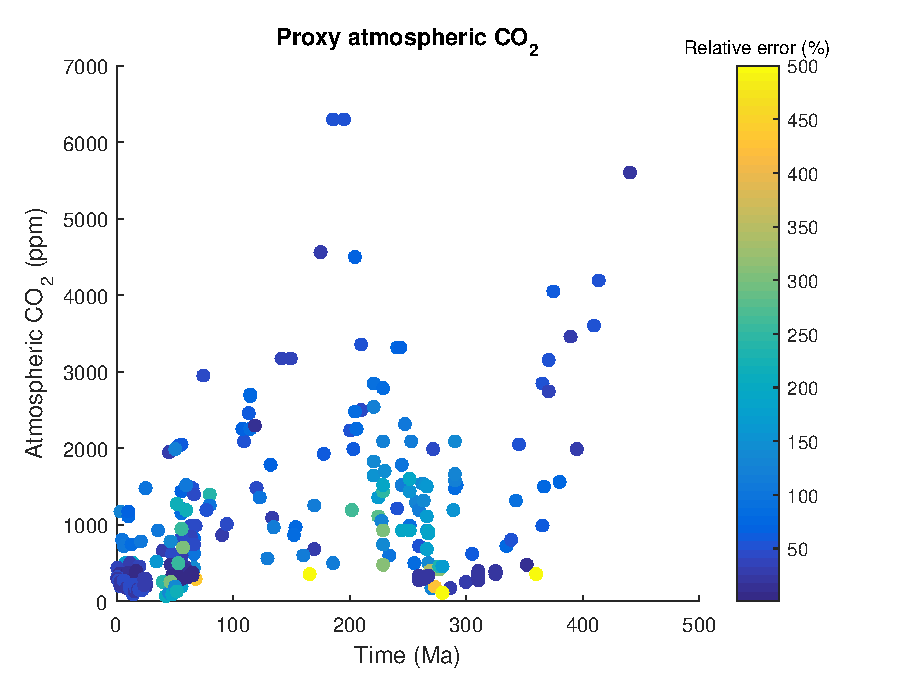
\includegraphics[width=\linewidth]{plot-CO2scatter4.eps}
\caption{Proxy reconstructed past variability in atmospheric CO2 (scatter plot).}
\label{fig:plot-CO2scatter4}
\end{marginfigure} 

\subsection{Other data filtering}

\noindent In the example of the observational Riverside temperature data (data file: \texttt{temperature\_riverside.txt}), if would be nice to also be able to use \docenv{find} ... which can indeed determine all the locations at which a \texttt{NaN} occurs\sidenote{Using \docenv{isnan}.}, by e.g.:

\begin{docspec}
>> find(isnan(temperature\_riverside))
\end{docspec}

\noindent ... but it is not obvious what to 'do' with the resulting list of linear indices for each cell containing a missing value (\texttt{NaN}). For instance, you cannot remove a single cell from a \(a\times b\) array for which both \(a\) and \(b\) are \(>1\) (because an array must contain the same number of elements in each row (and the same number of elements in each column)).

What you need, is a way of automatically removing each and every row in which one (or more) \texttt{NaN}s appear. There are two obvious approaches:

\vspace{2mm}
\textbf{1. use a loop}
\vspace{2mm}

We could go through the array, row by row, and for every row in which a \texttt{NaN} occurs, remove that row. The code would look something like:

\begin{docspec}
\textcolor[rgb]{0,0.501961,0}{\%\%\% script to load in data and remove NaN-containing rows}\\
\textcolor[rgb]{0,0.501961,0}{\% load dataset}\\
data=load(\textcolor[rgb]{1,0,1}{'temperature\_riverside.txt'},\textcolor[rgb]{1,0,1}{'ascii'});\\
\textcolor[rgb]{0,0.501961,0}{\% determine number of rows of data}\\
n\_max = length(data);\\
\textcolor[rgb]{0,0.501961,0}{\% initialize row count to the first row}\\
n = 1;\\
\textcolor[rgb]{0,0.501961,0}{\% loop through all rows}\\
\textcolor{blue}{while} (n <= n\_max),\\
\ \ \    found\_nans = find(isnan(data(n,:)));\\
\ \ \    \textcolor{blue}{if} (\(\sim\)isempty(found\_nans));\\
\ \ \ \ \ \        \textcolor[rgb]{0,0.501961,0}{\% remove row}\\
\ \ \ \ \ \        data(n,:) = [];\\
\ \ \ \ \ \        \textcolor[rgb]{0,0.501961,0}{\% remember to update total number of rows!!!}\\
\ \ \ \ \ \        n\_max = n\_max - 1;\\
\ \ \ \ \ \        \textcolor[rgb]{0,0.501961,0}{\% NOTE: don't update row count}\\
\ \ \    \textcolor{blue}{else}\\
\ \ \ \ \ \        \textcolor[rgb]{0,0.501961,0}{\% move on to next row}\\
\ \ \ \ \ \        n = n+1;\\
\ \ \    \textcolor{blue}{end}\\
\textcolor{blue}{end}\\
\end{docspec}

\vspace{2mm}
\textbf{2. cheat!}
\vspace{2mm}

(not really)

There is a relatively new \textbf{MATLAB} \textit{function} that achieves just this: \docenv{rmmissing}. Slightly simpler code to do the same job would then look like:

\begin{docspec}
\textcolor[rgb]{0,0.501961,0}{\%\%\% alt script to load in data and remove NaN-containing rows}\\
\textcolor[rgb]{0,0.501961,0}{\% load dataset}\\
data=load(\textcolor[rgb]{1,0,1}{'temperature\_riverside.txt'},\textcolor[rgb]{1,0,1}{'ascii'});\\
\textcolor[rgb]{0,0.501961,0}{\% remove problem rows!!!}\\
data = rmmissing(data);
\end{docspec}

\marginnote[-2.5in]{\begin{mdframed}[backgroundcolor=gray!10, roundcorner=10pt,leftmargin=1, rightmargin=1, innerleftmargin=5, innerrightmargin=5, innertopmargin=5,innerbottommargin=5, outerlinewidth=1, linecolor=light-gray]
\docenvdef{rmmissing} -- 'Remove rows or columns with missing entries'.
\\In the simplest usage:
\begin{docspecmargin}
B = rmmissing(A);
\end{docspecmargin}
Removes rows containing missing data elements from array \texttt{A}, assigning the results to array \texttt{B}.
\\MATLAB defines missing data as:
\begin{itemize}[noitemsep]
\item \texttt{NaN} - for number arrays
\item \texttt{<missing>} - for string arrays
\item blank character \texttt{[' ']} - for character arrays
\item empty character \texttt{{''}} - for cell arrays
\end{itemize}
(see \textbf{help} for further information and examples)
\end{mdframed}}

%------------------------------------------------

\subsection{Basic (pretend) 'stats'}

We are not going to delve into complex stats here. A variety of stats related functions are included in the \textbf{MATLAB Statistics Toolbox}. We'' stick to some simply functions included as standard in the basic package.

Useful basic stats-related functions include:

\begin{itemize}[noitemsep]
\setlength{\itemindent}{.2in}
\item \texttt{sum} -- the sum of a vector of numbers.
\item \texttt{mean} -- the mean of a vector of numbers.
\item \texttt{min} -- the minimum value of ...
\item \texttt{max} -- the maximum value of ...
\end{itemize}

In addition to which, basic \textbf{MATLAB} functions also include:

\begin{itemize}[noitemsep]
\setlength{\itemindent}{.2in}
\item \texttt{std} -- the standard deviations of a vector of numbers.
\item \texttt{var} -- the variance of a vector of numbers.
\item \texttt{median} -- the median value of ...
\item \texttt{mode} -- the mode value of ...
\end{itemize}

For instance, consider vector \texttt{A} (integers from 1 to 9, inclusive):

\begin{docspec}
>> A = [1:9];
\end{docspec}

Try out all of the above functions on the vector. Most of the values you can pretty much guess. The \texttt{mode} of the vector is perhaps the only one where it comes up oddly, because the mode of a set of values is defined as the most popular value, yet you have created only one of each value in the vector. So all values are in theory equally the most frequent and \textbf{MATLAB} simply returns the first.

So try adjusting the vector, adding an additional '7' at the end:

\begin{docspec}
>> B = [A 7];
\end{docspec}

\noindent Now what is the mode value of the vector \texttt{B}?

Sometimes you have have the situation where you have one or more \texttt{NaN}s in the data. For example:

\begin{docspec}
>> C = [A NaN];
\end{docspec}

\noindent Now try out some of the same functions on vector \texttt{C}. What happens? Why \textbf{MATLAB} does this and does not simply ignore \texttt{NaN}s, is anypony's guess. I mean, what application could you possibly have where when you ask for the mean of a vector, you are hoping to be told '\texttt{NaN}'? There are solutions.

\begin{enumerate}[noitemsep]
\setlength{\itemindent}{.2in}
\item Firstly -- you could use find, to find and remove \texttt{NaN}s from data. So if you have data that includes \texttt{NaN}s, you could simply filter them out prior to processing the data. The function for determining whether or not an array element is a \texttt{NaN}, is \docenv{isnan} )see earlier Box).
\item Or you could create a loop and test each element in turn as to whether or not it is a \texttt{NaN} (again, using the \docenv{isnan} function).
\item The MATLAB functions listed above, all (most?) have an additional optional parameter (see Box) that allows you to direct \textbf{MATLAB} to ignore \texttt{NaN}s in the data.
\item Lastly, in the \textbf{Statistics Toolbox}, there are variants of all (most?) of these functions that automatically ignore \texttt{NaN}s, such as \texttt{nanmean} (the \texttt{NaN}-ignoring variant of \texttt{mean})
\end{enumerate}

Try out each of these solutions, applying them to the vector \texttt{C} (or a \texttt{NaN}-containing vector of your choice).

All of these functions can also be used on 2D arrays (matrices) ... with care. Consider the matrix:

\begin{docspec}
>> D = [1 2 3; 4 5 6; 7 8 9];
\end{docspec}

\noindent (which has the same elements as \texttt{A}, just in a different configuration). What happens when you ask for \texttt{mean(D)}? As per help (and the Box): '\textit{If A is a matrix, then mean(A) returns a row vector containing the mean of each column.}' So \texttt{mean(D)} is returning the mean of \texttt{[1 4 7]}, \texttt{[2 5 8]}, and \texttt{[3 6 9]}. Try \textit{transposing} the matrix and then using the \texttt{mean} \textit{function}. You should see that you now get the mean of the individual rows (rather than columns) of matrix \texttt{D}:

\begin{docspec}
>> mean(D')\\
ans =\\
\ \ \ 2     5     8
\end{docspec}

This goes for \texttt{sum} and all (most?) the rest of the functions.

If you need the total sum of all the elements in a matrix, or mean of all the elements in a matrix, you can simply \textit{nest} the \textit{functions}:

\begin{docspec}
>> sum(sum(D))
\end{docspec}

\noindent or if you prefer breaking things down into sperate steps:

\begin{docspec}
>> E = sum(D);
>> sum(E)
\end{docspec}

\noindent However, note that \texttt{std(std(D))} is not the standard deviation of all elements in the matrix \texttt{D}. Why?

%------------------------------------------------

\subsection{Some useful data manipulations techniques}

This (failure to directly obtain the standard deviation of all the elements in a matrix) brings us to array manipulation, which will prove useful in other contexts, such as graphing and particularly scatter plots. In the previous example, \texttt{std(std(D))} fails to give us what we want. Ideally, we would like to have all the elements of D reconfigured so that they were in a single vector format, and we could just write e.g. \texttt{std(D)} and get a single, complete answer.

\marginnote[-4.00in]{\begin{mdframed}[backgroundcolor=gray!10, roundcorner=10pt,leftmargin=1, rightmargin=1, innerleftmargin=5, innerrightmargin=5, innertopmargin=5,innerbottommargin=5, outerlinewidth=1, linecolor=light-gray]
\docenvdef{reshape}
\\Use \docenv{reshape} to transform data in an array of one shape (i.e. configurations of rows and columns), into another. \textbf{MATLAB} \texttt{help} is OK on this and for the main usage of the \textit{function}, says:
\\\textit{'B = reshape(A,sz) reshapes A using the size vector, sz, to define size(B). For example, reshape(A,[2,3]) reshapes A into a 2-by-3 matrix.}'
\\In this usage you need to specify the rows and columns of the resulting array.
\\NOTE that the array you turn it into to, can have a single row, or a single column (and hence be a vector), but you need to specify this with a \texttt{1}.
\\Also note that the total number of elements in the array must be conserved, so if you turn an \(n\times m\) array into a \(p\times p\) array, then it must be true that:
\\\(n\times m = o\times p\)
There is also a convenient second usage, that will attempt to automatically determine the row or columns needed to make \(n\times m = o\times p\) true, given either \(o\) or \(p\). For example:
\begin{docspecmargin}
B = reshape(A,2,[])
\end{docspecmargin}
in the previous example will automatically determine that 3 columns are needed. Conversely,
\begin{docspecmargin}
B = reshape(A,[],3)
\end{docspecmargin}
will determine that 2 rows are required to meet the \(n\times m = o\times p\) criteria.
\\This usage is particularly convenient for making vectors, e.g.:
\begin{docspecmargin}
B = reshape(A,[],1)
\end{docspecmargin}
\end{mdframed}}

\textbf{MATLAB} provides the function \docenvdef{reshape}\sidenote{See \texttt{help} and Box} for the express purpose of re-configuring the shape of an \textit{array}, such as turning a \textit{matrix} into a \textit{vector}, or \textit{vice versa}. For instance, given the \(3x3\) matrix \texttt{D} in the previous example:

\vspace{2mm}
\(\begin{pmatrix}
1 & 2 & 3 \\
4 & 5 & 6 \\
7 & 8 & 9 \\
\end{pmatrix}\)
\vspace{2mm}

how do we turn this into a \(9x1\) column vector?

\vspace{2mm}
\(\begin{pmatrix}
1 \\
4 \\
7 \\
2 \\
5 \\
8 \\
3 \\
6 \\
9 \\
\end{pmatrix}\)
\vspace{4mm}

You can use \docenv{reshape} in 2 different ways:

\begin{enumerate}[noitemsep]
\setlength{\itemindent}{.2in}
\item Firstly, you can explicitly specify the new array shape you want.\sidenote{Obviously, the total number of elements in the array \uline{must} be conserved.} e.g.
\begin{docspec}
Dvector = reshape(D,[9,1]);
\end{docspec}
\item Alternatively, if you know you want a single column vector and cannot be bothered to work out how many rows you need, MATLAB will kindly pick up the slack via a slightly different usage of \texttt{reshape}:
\begin{docspec}
Dvector = reshape(D,[],1);
\end{docspec}
Here you are specifying one column, but 'whatever' (\texttt{[]}) rows.
\end{enumerate}

\noindent(Having created a vector containing all the numbers, you can now find the standard deviation: \texttt{std(Dvector)}.)

Obviously, if you want a row, rather than a column vector -- either transpose the column vector to row vector shape, or specify the format of a row vector in the first place when using \texttt{reshape}:

\begin{docspec}
Dvector = reshape(D,[1,9]);
\end{docspec}

Lastly, you might notice how MATLAB reads the elements from D before creating the new array shape -- elements are read from the top of the first column downwards, before moving to column \#2. Hence why the order of numbers is 1  4  7  2  5  8 ... 

What, instead, if you wanted a vector with the ordering:

\vspace{2mm}
\(\begin{pmatrix}
1 \\
2 \\
3 \\
4 \\
5 \\
6 \\
7 \\
8 \\
9 \\
\end{pmatrix}\)
\vspace{4mm}

?

ANS: simply \textit{transpose} the matrix before you reshape:

\begin{docspec}
Dvector = reshape(D',[1,9])
\end{docspec}

\noindent (or \texttt{Dvector = reshape(transpose(D),[1,9])}).

%------------------------------------------------

\subsection{Data interpolation}

Interpolation? What is it and why would you do it? We'll answer this via an example. 

First download the ice-core dataset of atmospheric CO2 over the past ~800,000 years, recovered from the Dome C site on Antarctica -- filename \textsf{icecore\_co2.txt} on the course webpage. Start by plotting it (your choice of \textbf{MATLAB} plotting function) to see what you are dealing with.\sidenote{First column / x-axis values are age, in years, and 2nd column / y-axis values are CO2 concentration, in units of ppm.}

So what if we wanted to know the average (mean) value of atmospheric \(CO_{2}\) over the last full glacial cycle, i.e. between now (age zero) and the end of the previous interglacial period, about 115,000 years ago.

So firstly, you might use your most excellent MATLAB skills to extract all the data corresponding to this specific interval -- i.e. all the ages (and corresponding \(CO_{2}\) values, between zero and 115,000 years, or rather, \uline{less than or equal to} 115,000 years. You should know this requires the find function, and that the range of indices if given by (assuming the data array you loaded in is called \texttt{co2}):

\begin{docspec}
a=find(co2(:,1)<=115000)
\end{docspec}

\noindent which simply says: take all the elements in the 1st column of the array \texttt{co2} (\texttt{co2(:,1)}), and find the indices of all the elements with a value equal or less than 115,000. To select just the first 115000 years of data in \texttt{co2} is then just a matter of: 

\begin{docspec}
co22=co2(a,:)
\end{docspec}

\noindent and check that this does indeed give you the correct portion of data and has assigned it to the array \texttt{co2new}.
(Maybe plot to confirm.)

It is worth pausing at this point -- this is a common, and powerful, usage of \texttt{find}, and of \textit{indexing}, and you should be sure you understand it before moving on. What this line is saying is: take both columns of the array \texttt{co2} -- select all the elements (rows) defined by the vector \texttt{a}, and assign the result to \texttt{co2new}.

OK, so we are progressing well towards answering the question -- the mean \(CO_{2}\) value over the last glacial cycle (last 115,000 years). In fact -- try answering that now (using \texttt{mean}). You should end up with a value of \(245 ppm\).\sidenote{Note that \textbf{MATLAB} will report the value in a scientific notation with a power (here \(10^{2}\)).} The question is -- do you 'believe' it? Look at the plot -- do you think that value is representative of the average?

To make the problem more obvious -- repeat the above exercise, but now consider only the past 40,000 years. From the plot, high, interglacial \(CO_{2}\) values characterise only the last 10,000 years or so, with a transition over 5,000 years or so before that. From 15,000 years and back to 40,000, \(CO_{2}\) is clearly bumping along its lowest values. What would you guess the mean \(CO_{2}\) value is? Now try it. I get \(249 ppm\) \(CO_{2}\). Does that look correct to you, across the past 40,000 years?

If you were previously using \texttt{plot} to plot the data, now try \texttt{scatter}. It should be much more obvious what is going on now -- you have very uneven data sampling in time -- the bulk of the data is from the last 10,000 years or so, and there are very few data points older than about 22,000 years. When \textbf{MATLAB} calculates a mean, it is off the data points, and an uneven data sampling will give a biased, unrepresentative value. We need to \uline{interpolate} the data -- place it on an evenly sampled-in-time basis.

The \textbf{MATLAB} function to interpolate vector (1D) data is \docenvdef{interp1} (see \texttt{help}/Box).

\marginnote[-2.5in]{\begin{mdframed}[backgroundcolor=gray!10, roundcorner=10pt,leftmargin=1, rightmargin=1, innerleftmargin=5, innerrightmargin=5, innertopmargin=5,innerbottommargin=5, outerlinewidth=1, linecolor=light-gray]
\docenvdef{interp1}
\begin{docspecmargin}
yi = interp1(x,y,xi)
\end{docspecmargin}
will interpolate the y-axis values located at x-axis points given by the vector \texttt{x}, onto the x-axis points given by vector \texttt{xi}. The resulting interpolated y-values are assigned back to \texttt{yi}.
\\By default the interpolation methods used is linear. For a different interpolation method, use the varient of the function:
\begin{docspecmargin}
yi = interp1(x,y,xi,method)
\end{docspecmargin}
where method is one of: \texttt{'nearest'}, \texttt{'linear'}, \texttt{'spline'}, \texttt{'cubic'} ... (for a fuller list, see \texttt{help}).
\\To extrapolate outside of the domain spanned by the (original) x-axis vector \texttt{x}, specify:
\begin{docspecmargin}
yi = interp1(x,y,xi,method,'extrap')
\end{docspecmargin}
\end{mdframed}}

The first thing we need, to use \docenv{interp1}, is a vector of points in time, that we are going to interpolate our data on to. As a rule, the vector should ideally not extend in value beyond the minimum and maximum values of the original axis, but we'll ignore this for now. We might pick ... 1,000 years as a simple sampling interval, and so to create this new axis vector, we would write:

\begin{docspec}
xi=[0:1000:40000];
\end{docspec}

\noindent assuming we stick with the 0-40,000 year interval. The \docenv{interp1} function requires that you pass this vector, along with the original time (x-axis) vector, and the original data (y-axis) vector, and will give you a new data vector, with values corresponding to the time points defined by \texttt{xi}. Like this:

\begin{docspec}
yi=interp1(co22(:,1),co22(:,2),xi);
\end{docspec}

\noindent If you prefer to break things down\sidenote{And then you might also make the variable names REALLY explicit, and have \texttt{xold}, \texttt{yold}, \texttt{xnew}, \texttt{ynew} or something.} so as the process is clearer, maybe first extract and create the original data, x-axis (time) vector:

\begin{docspec}
xold=co22(:,1);
\end{docspec}

\noindent and then the y-axis (data) vector:

\begin{docspec}
yold=co22(:,2);
\end{docspec}

\noindent and then do the interpolation:

\begin{docspec}
y1=interp1(xold,yold,x1);
\end{docspec}

\noindent Either way, now scatter-plotting the interpolated data:

\begin{docspec}
scatter(x,y);
\end{docspec}

\noindent should result in an obviously evenly-spaced data plot.

We could now use mean, except if you were paying attention, because we extrapolated outside of the range of the extracted data into the array \texttt{co2new}. But you know how to handle this situation, i.e. removing the offending \texttt{NaN} rows, or use \texttt{nanmean} if you have access to the required \textbf{MATLAB} toolbox.

Or, you could re-do the interpolation, but interpolate from the full, original data array, which you know extends way past 40,000 years. And ... specify the very first time point as 1,000 years rather than zero. e.g.

\begin{docspec}
x1=[1000:1000:40000];\\
y1=interp1(co2(:,1),co2(:,2),x1); 
\end{docspec}

Well ... it doesn't work, which is sort of pretty 'real world' problem-esk. The issue is that there is a duplicate year -- i.e. 2 \(CO_{2}\) values with the same year.\sidenote{The \textbf{MATLAB} interpolation function requires a strictly monotonically increasing (with no duplicates) old and new x-axis vector.} How to find them? Well, you saw earlier the function \texttt{mode}, which return the most popular value in an array. If we do:

\begin{docspec}
>> mode(co2(:,1))\\
ans =\\
\ \ \ 409383
\end{docspec}

Ha ha, so the year 409,383 is duplicated.\sidenote{The absence of duplicated year values, or rather, there only being one of each individual number, would result in \textbf{MATLAB} returning the very first value in the vector. The only confusion here would be if the very first value was itself duplicated ...} How to find this ...

\begin{docspec}
find(co2(:,1)==409383);
\end{docspec}

\noindent or if you prefer (and neater):
\begin{docspec}
>> rows=find(co2(:,1)==mode(co2(:,1)))\\
ans =\\
\ \ \ 531\\
\ \ \ 532\\
\end{docspec}

\noindent giving us the row numbers. We could be cleaver, and create a single entry for this year, with the \(CO_{2}\) value formed of the mean of the duplicate entries:

\begin{docspec}
co2mean=mean(co2(rows,2));
\end{docspec}

\noindent replace the first \(CO_{2}\) value ...

\begin{docspec}
co2(rows(1),2)=co2mean;
\end{docspec}

\noindent ... and then delete the second.

\begin{docspec}
co2(rows(2),:)=[];
\end{docspec}

Phew! Now try the interpolation again. Plot (\texttt{scatter} and/or \texttt{plot}). Find the mean \(CO_{2}\) value over 0-40,000 (technically, now we have restricted the data to 1,000-40,000). Does this seem more reasonable? Repeat for 0-115,000 years (or 1,000-115,000 years). Also try out carrying out an interpolation with closer spacing, say 500 or 100 years.

Finally, if you read the (Box or \texttt{help}) details about the function \texttt{interp1}, the more recent \textbf{MATLAB} version releases enable you to extrapolate outside of the data domain. SO instead of having to restrict the \texttt{xi} vector to starting at year 1,000, you can start at year zero:

\begin{docspec}
x1=[0:1000:40000];\\
y1=interp1(co2(:,1),co2(:,2),x,'linear','extrap'); 
\end{docspec}

%------------------------------------------------

\newpage

%------------------------------------------------

\section{Even nicer graphing and graphics}

There are a bunch of simple \textbf{MATLAB} drawing and text placement commands that can help improve the look and feel of scientific plots, or even replace the provided plotting functions (i.e. you can create your own bespoke plotting functions). There are also a variety of options for altering the axes, axes tick-marks, axes tick-mark labels, etc that can be useful.

%------------------------------------------------

\newpage

%------------------------------------------------

\subsection{Drawing lines and shapes}

We'll start with some simply line and shape drawing. At the command line -- open a new \textsf{figure window} (\texttt{>> figure;}). Before anything else, do a \texttt{>> hold on;}).

When \textbf{MATLAB} draws lines and shapes and places text, it needs to know the coordinates of where to place things. It is not possible (I think) to draw directly in the \textsf{figure window} -- \textbf{MATLAB} needs a frame to put things in, and the easiest way to do this is to create a set of axes. So having opened a new \textsf{figure window}, set the range of the x- and y-axes
\sidenote{Here taking the example range of 0-100 on both axes.}:

\begin{docspec}
>> axis([0 100 0 100]);
\end{docspec}

\noindent The resulting figure is really not very exciting ... and should look like Figure \ref{fig:ch3-graphics01}.

\begin{marginfigure}[0.0in]
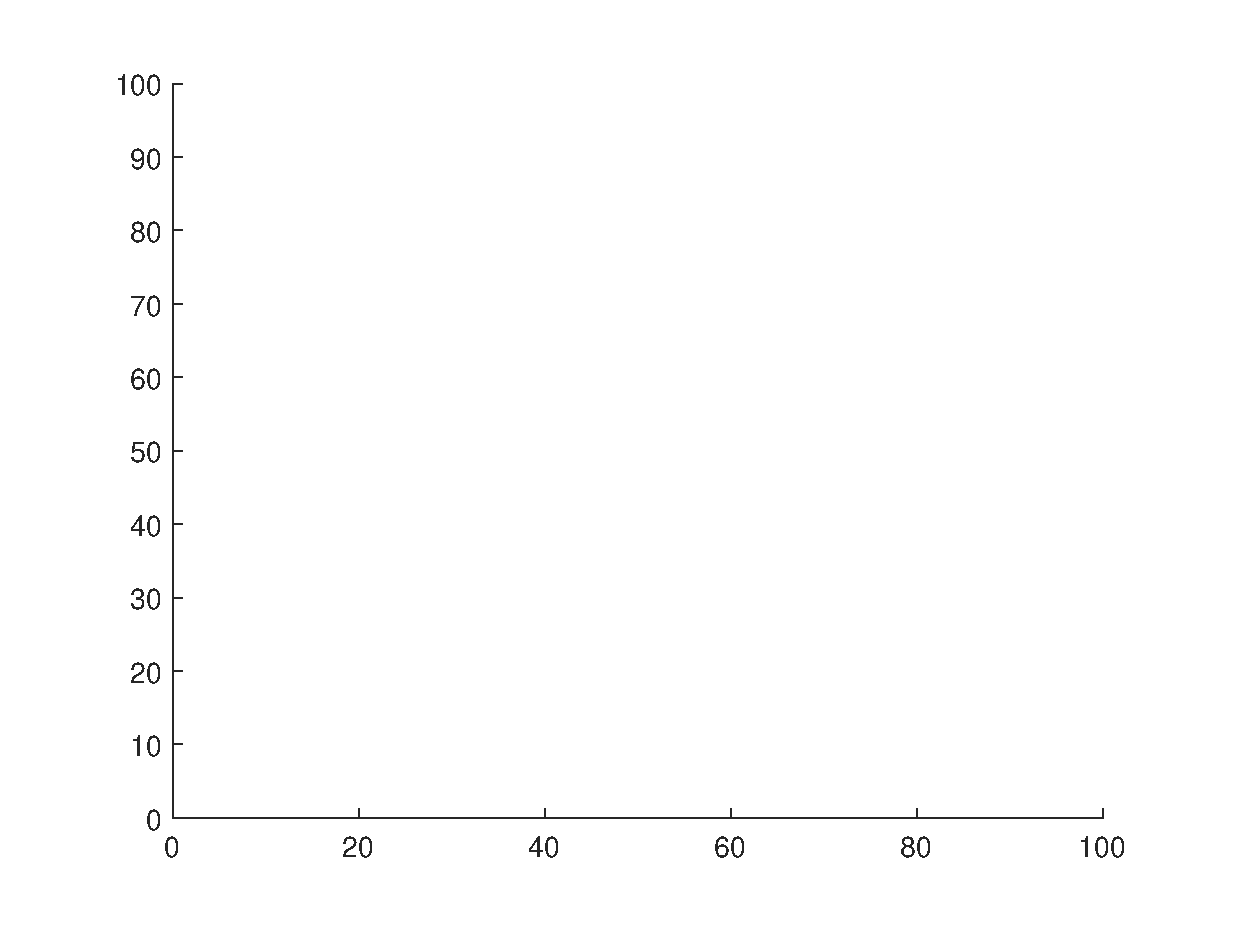
\includegraphics[width=\linewidth]{ch3-graphics01.eps}
\caption{Figure window with axes.}
\label{fig:ch3-graphics01}
\end{marginfigure}

\vspace{1mm}
\noindent\rule{4cm}{0.5pt}
\vspace{2mm}

\noindent There are 2 ways to draw a line:

\begin{enumerate}[noitemsep]

\item \texttt{plot}
\\Are you recall, \texttt{plot} will plot a sequence of (x,y) points, and by default, join them up with a line. If we wanted a diagonal line, from the original to the mid-point of the plot area, we could invent a pair of vectors to define the two points we need -- at (0,0) and (50,50):
\begin{docspec}
X1 = [0 50];\\
Y1 = [0 50];
\end{docspec}
and then plot the resulting points as a \texttt{plot} plot:
\begin{docspec}
plot(X1,Y1);
\end{docspec}
You should now see something like Figure \ref{fig:ch3-graphics02}.\sidenote[][-0.0in]{If you find that the plot area has been re-sized such that the x- and y-axes now both go from 0-50, then you have forgotten to do a \texttt{hold on}.}

\marginnote{\begin{mdframed}[backgroundcolor=gray!10, roundcorner=10pt,leftmargin=1, rightmargin=1, innerleftmargin=5, innerrightmargin=5, innertopmargin=5,innerbottommargin=5, outerlinewidth=1, linecolor=light-gray]
\docenvdef{line}
To draw a simple (single) line on a graphic:
\begin{docspecmargin}
>> line([x1 x2],[y1 y2])
\end{docspecmargin}
where \texttt{x1} and \texttt{x2} are the \textit{x}-coordinates of the start and end position of the line, and \texttt{y1} and \texttt{y2} are the corresponding \textit{y}-coordinate values.
\end{mdframed}}

\item \texttt{line}
\\\textbf{MATLAB} provide a specific command for drawing lines ... \docenvdef{line}. In its simplest usage, it is a little like \texttt{plot}, except taking only a single pair of x- and y-coordinate values.
\\To use \texttt{line} to draw a 2nd line segment, starting at (50,50) and terminating at (100,0), we create another pair of vectors to define these points:
\begin{docspec}
X2 = [50 100];\\
Y2 = [50 0];
\end{docspec}
and then draw it:
\begin{docspec}
line(X2,Y2);
\end{docspec}
as shown in Figure \ref{fig:ch3-graphics03}.
\end{enumerate}

\noindent Obviously, both line segments could be drawn using \texttt{plot}, or both with \texttt{line}.

\begin{marginfigure}[0.5in]
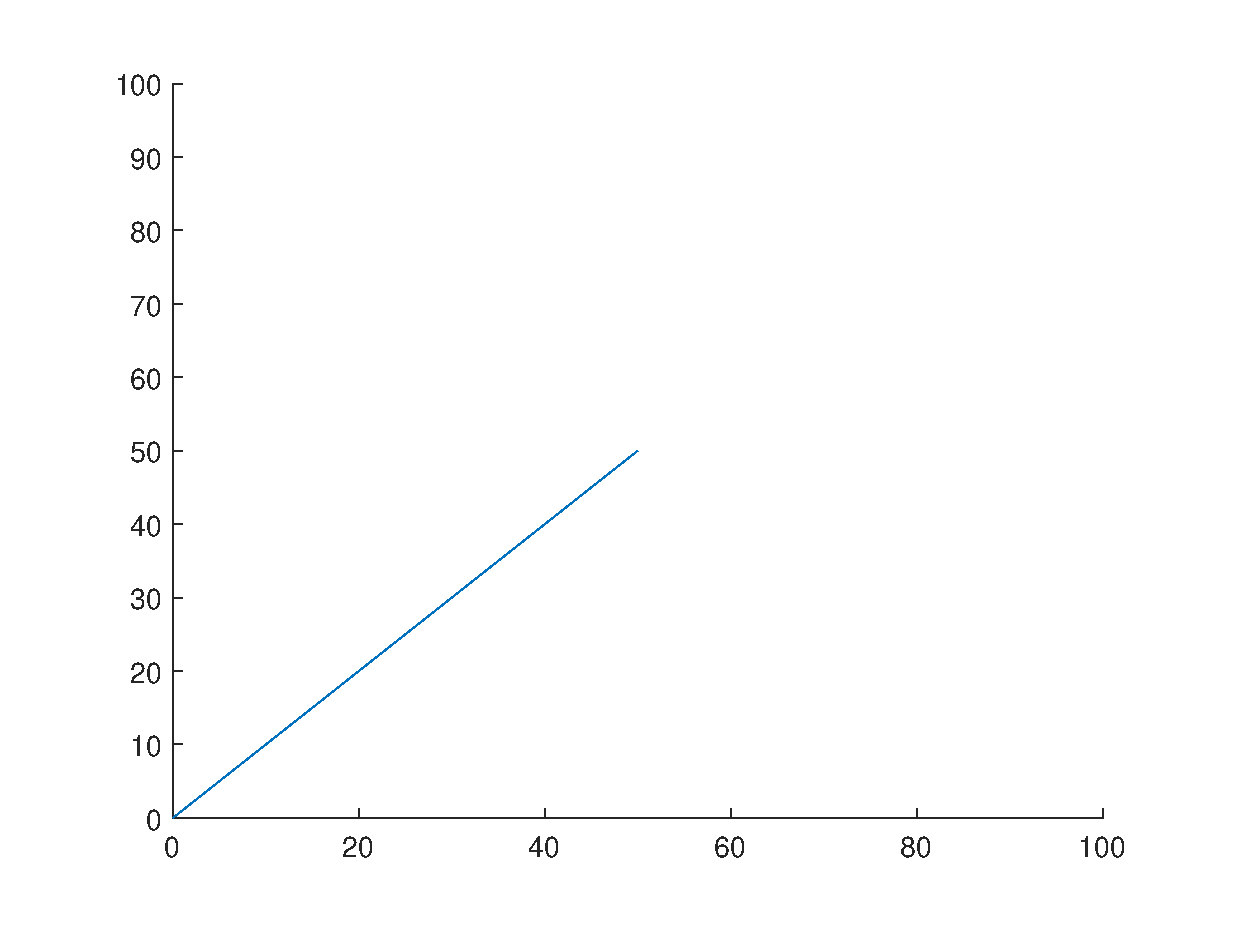
\includegraphics[width=\linewidth]{ch3-graphics02.eps}
\caption{Figure window with single line segment (via \texttt{plot}).}
\label{fig:ch3-graphics02}
\end{marginfigure}

\begin{marginfigure}[0.0in]
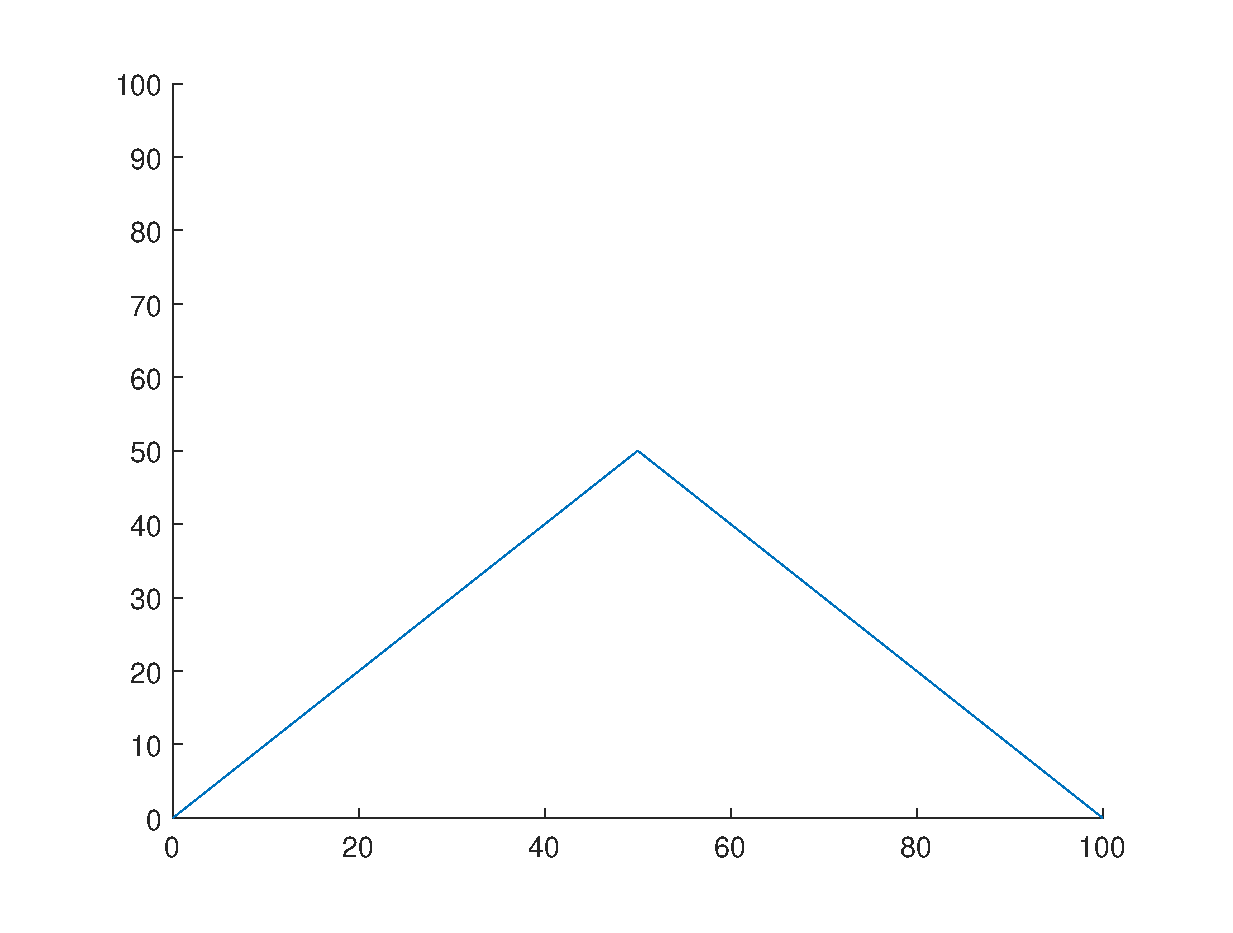
\includegraphics[width=\linewidth]{ch3-graphics03.eps}
\caption{Figure window with a second line segment (via \texttt{line}).}
\label{fig:ch3-graphics03}
\end{marginfigure}

\vspace{1mm}
\noindent\rule{4cm}{0.5pt}
\vspace{2mm}

\noindent If you are just drawing, rather than annotating a plot with axes, then you might want to turn off, or hide, the axes tick marks and tick labels. To do this, we first need to find the special \textbf{MATLAB} ID of the axes, which helpfully, because you only have one set of axes and have just been using them, is the 'current axis'. To do this, we use the \docenvdef{gca} function, which returns the \textit{handle} (ID) of the axes:

\begin{docspec}
>> h = gca;
\end{docspec}

\noindent Having got the axis \textit{handle}\sidenote[][2.0in]{It is worth omitting the \texttt{;} in order to see the properties associated with the axes, and in fact, it is worth clicking on \texttt{Show \uline{\textcolor{blue}{all properties}}} to see a list of everything that can be edited and adjusted. \\ALL these can be changed if you ever want!!!}, we can now 'set' the properties of the axes, using \docenvdef{set}:

\begin{docspec}
>> set(h,'XTick',[],'XTickLabel','');
\end{docspec}

What this does is to tell \textbf{MATLAB}: take the graphics object with the ID contained in variable \texttt{h} (which we just retried via the \texttt{gca} function), and set (whcih is why we use the command \texttt{set} ...) the following properties:

\begin{itemize}[noitemsep]
\setlength{\itemindent}{.2in}
\item \texttt{'XTick',[]} -- set the number and position of tick marks on the x-axis, to the contents of the empty vector \texttt{[]}.
\item \texttt{'XTickLabel',''} -- set the labels applied to the tick-marks, to \texttt{''} (i.e. no text).
\end{itemize}

\noindent Actually, in this example, the 2nd graphics parameter set (the labels) is sort of redundant, as there are no tick-marks in the first place ... 

To see how different combinations of settings pan out, try:

\begin{docspec}
>> set(h,'XTick',[0 50 100],'XTickLabel','');
\end{docspec}
(3 small inwards ticks, no labels)

\begin{docspec}
>> set(h,'XTick',[0 50 100],'XTickLabel','cat');
\end{docspec}
:o)
\\\noindent or:

\begin{docspec}
>> set(h,'XTick',[0 50 100],'XTickLabel',\{'cat', 'dog', 'rabbit'\});
\end{docspec}
where \texttt{\{'cat', 'dog', 'rabbit'\}} is actually a 3 string \textit{cell array}.

All this insanity should be looking like Figure \ref{fig:ch3-graphics04} (if we also remove the y-axis ticks and labels\sidenote[][-1.5in]{It is sufficient just to type: \begin{docspecmargin}>> set(h,'YTick',[]);
\end{docspecmargin}}).

\begin{marginfigure}[-1.0in]
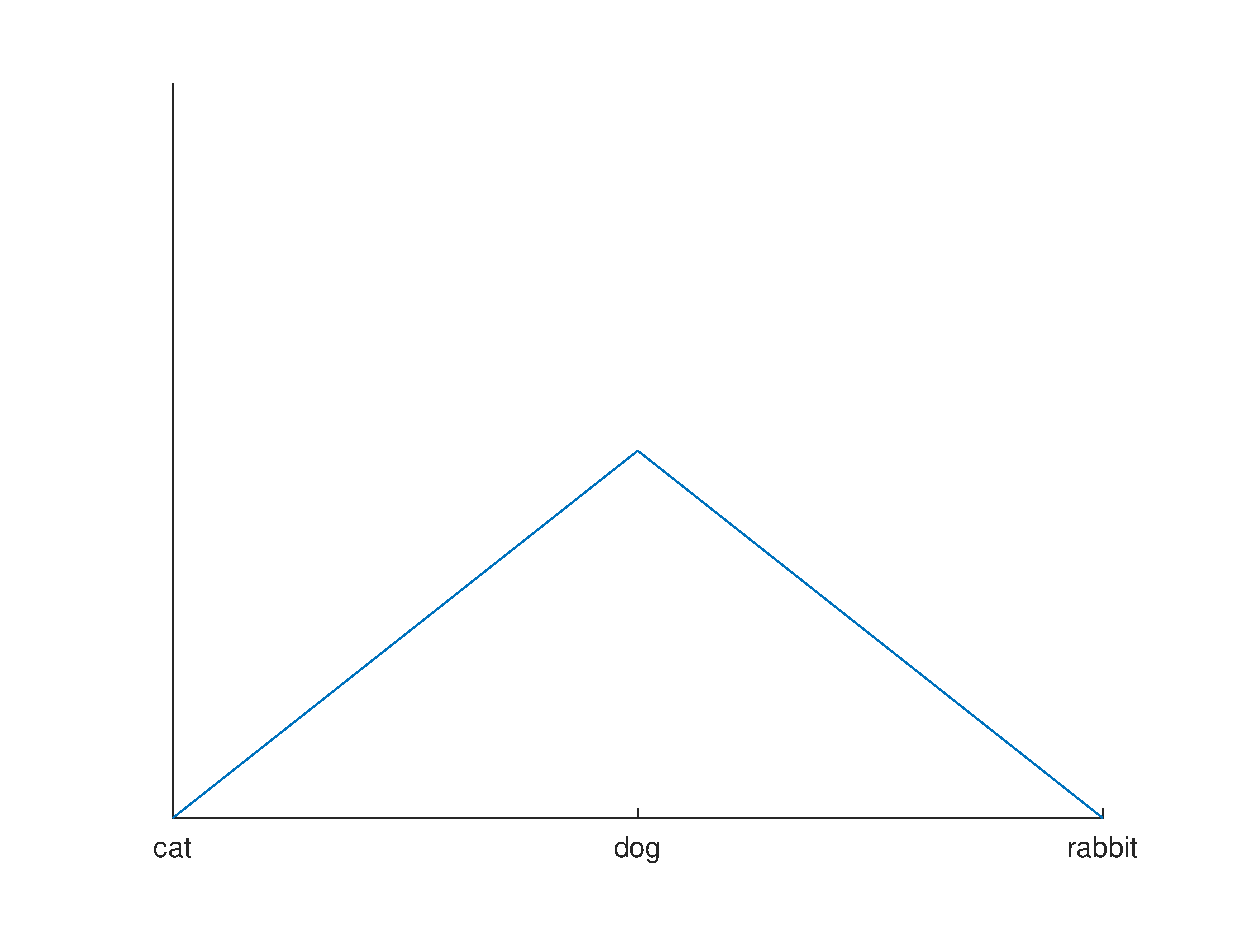
\includegraphics[width=\linewidth]{ch3-graphics04.eps}
\caption{(no comment).}
\label{fig:ch3-graphics04}
\end{marginfigure}

An alternative way to create a figure to draw on, without having to remove the axes ticks and labels etc etc, is to create the axes as invisible. To try this -- first create a new \textsf{figure window}.\sidenote{If you find yourself drowning in \textsf{figure window}s, remember that \texttt{close} closes the current window, and \texttt{close all} closes all of them.}

\begin{docspec}
>> h = axes('Position',[0 0 1 1],'Visible','off');
\end{docspec}
Here, \texttt{'Position',[0 0 1 1]} specifies that the axes area should fill the window, and \texttt{'Visible','off'} says to make the axes invisible. (We keep a copy of the \textit{handle}, \texttt{h}, just in case we need it later.) And set the axes as usual:
\begin{docspec}
axis([0 100 0 100]);
\end{docspec}

For some reason ... you need to do \texttt{hold on} only \uline{after} creating axes frame ...

\vspace{1mm}
\noindent\rule{4cm}{0.5pt}
\vspace{2mm}

\noindent The command \docenv{set} can be used in the context of any (I think?) graphics object, i.e. component part of a final plot (e.g. axis, ticks, line, point, etc). For example, in creating the line segment previously:
\begin{docspec}
h = line(X2,Y2);
\end{docspec}
you could store a copy of the \textit{handle} of that line segment. With this, you can now change the properties of the line (after you have drawn it).

\begin{itemize}[noitemsep]
\setlength{\itemindent}{.2in}
\item \texttt{set(h,'LineWidth',2.0);}
\\will change the line width to 2.0 (points). 
\item \texttt{set(h,'Color',[1 0 0]);}
\\will turn the line red, using the \textit{RGB} (red-green-blue) notation: \\\texttt{[1 0 0]}\sidenote{Alternatively:
\begin{docspecmargin}set(h,'Color','r');
\end{docspecmargin}}.
\item \texttt{set(h,'LineStyle',':');}
\\\noindent will make the line dotted. 
\end{itemize}

\vspace{1mm}
\noindent\rule{4cm}{0.5pt}
\vspace{2mm}

\noindent An obvious use for drawing lines on plots, is to annotate them. e.g. placing a text label (we'll see shortly), with a line pointing from the text to a specific feature. You can do with with a simple line and hence the \texttt{line} command.

It would be more handy and in fact common, to include an arrow head to make clear that the line is pointing to something. This can in theory be done by drawing 2 more, shorter lines, but is no fun at all\sidenote{True fact -- I have tried it :(}. \textbf{MATLAB} hence provides the function \docenvdef{quiver}. \texttt{quiver} is commonly used for plotting fields of arrows, but can equally be used to create a single arrow -- much like earlier you used \texttt{plot} to draw just a single pair of joined up points and hence a line. However, rather than take a pair of (x,y) points -- one for the start and one for the end, of the line, \texttt{quiver} takes an (x,y) location for the start of the arrow, and then the \uline{length} in the x and y directions.

Consistent with the previous example, we were starting the line segment at (0,0), and then extending the line to (50,50). The length vector in this case is also [50 50]. So, given the specific syntax and input parameter format required by \textbf{MATLAB} for this function, we would write:

\begin{docspec}
>> quiver(0,0,50,50,0);
\end{docspec}
The last, 5th parameter (\texttt{0}), telling \textbf{MATLAB} not to auto-scale the arrow.\sidenote{If it your arrow hard to make out -- try creating a new \textsf{figure window}. You can also use \texttt{cls} to clear all the graphics in the window (i.e. and not have to re-generate the \textsf{figure window}.}

\vspace{1mm}
\noindent\rule{4cm}{0.5pt}
\vspace{2mm}

\noindent For shapes, you can draw rectangles with \docenvdef{patch}. This takes as parameter input, a vector of x-coordinate positions, then a vector of y-coordinate positions, and as a 3rd parameter, the color for the object.

So in our previous example, with the x- and y-axes going from 0-100, say we want to draw a square in the middle, 20 units on each side. We could create our vector of x-axis coordinates as such:
\begin{docspec}
>> X1 = [40 40 60 60];
\end{docspec}
and for the y-axis ... some care is needed and often it might be helpful to sketch out the coordinate pairs and positions on a piece of paper:
\begin{docspec}
>> Y1 = [40 60 60 40];
\end{docspec}
And then:
\begin{docspec}
>> patch(X1,Y1,'r');
\end{docspec}
shown in Figure \ref{fig:ch3-shape01}.

\begin{marginfigure}[-2.0in]

\includegraphics[width=\linewidth]{ch3-shape01.eps}
\caption{Square.}
\label{fig:ch3-shape01}
\end{marginfigure}

Or we could re-orientate the square:nits on each side. We could create our vector of x-axis coordinates as such:
\begin{docspec}
>> X2 = [40 50 60 50];\\
>> Y2 = [50 60 50 40];
\end{docspec}
\begin{docspec}
>> patch(X2,Y2,'c');
\end{docspec}
shown in Figure \ref{fig:ch3-shape02}.

\begin{marginfigure}[-1.0in]
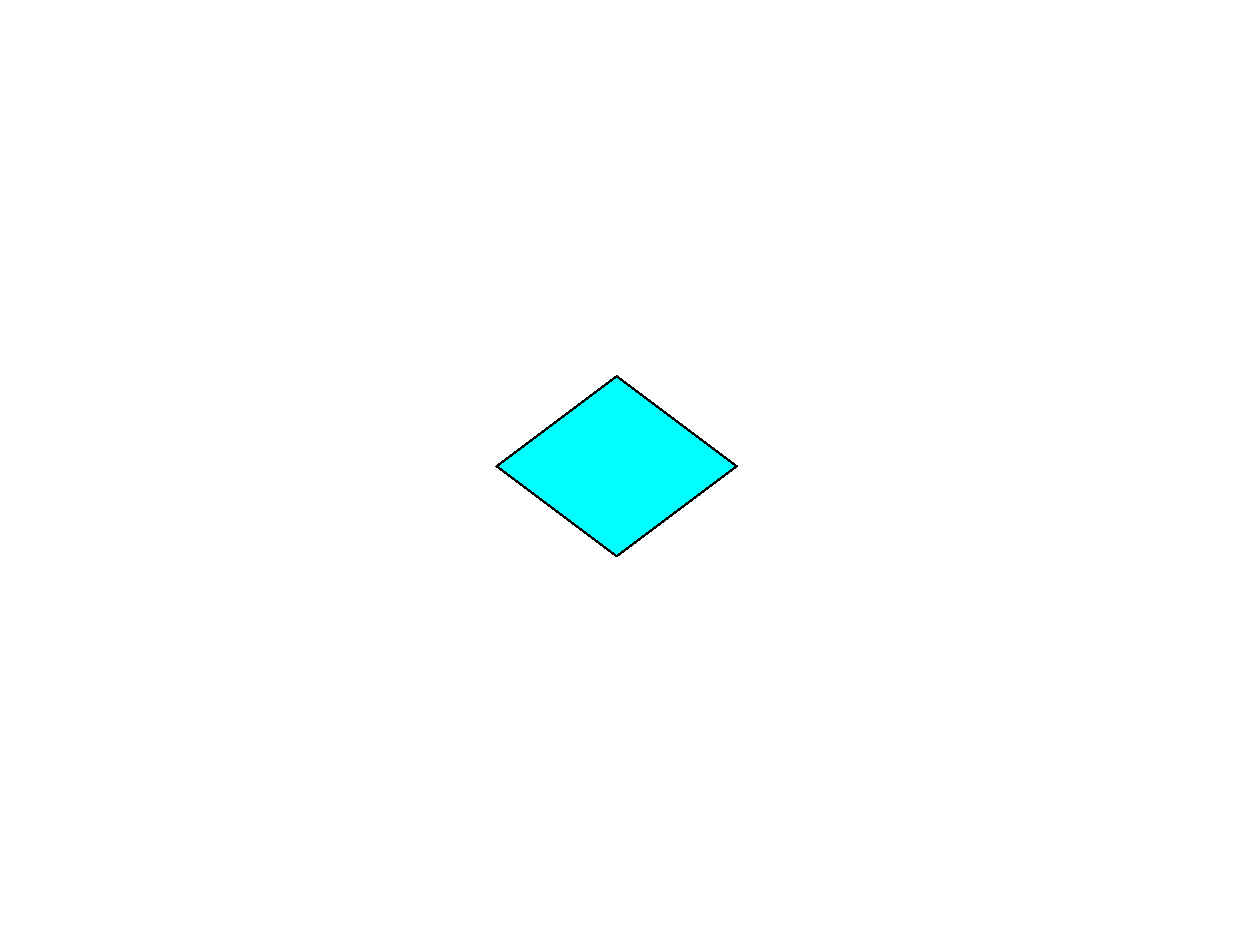
\includegraphics[width=\linewidth]{ch3-shape02.eps}
\caption{Alt square.}
\label{fig:ch3-shape02}
\end{marginfigure}

\texttt{patch} is in fact much more flexible than I have shown so far, and in fact, will draw \uline{any} polygon. Consider this sort of slightly random series of x and y coordinates: 
\begin{docspec}
>> X3 = [20 40 60 80 60 40];\\
>> Y3 = [50 60 50 60 40 30];
\end{docspec}
\begin{docspec}
>> patch(X3,Y3,'g');
\end{docspec}
gives Figure \ref{fig:ch3-shape03}.

\begin{marginfigure}[-0.0in]
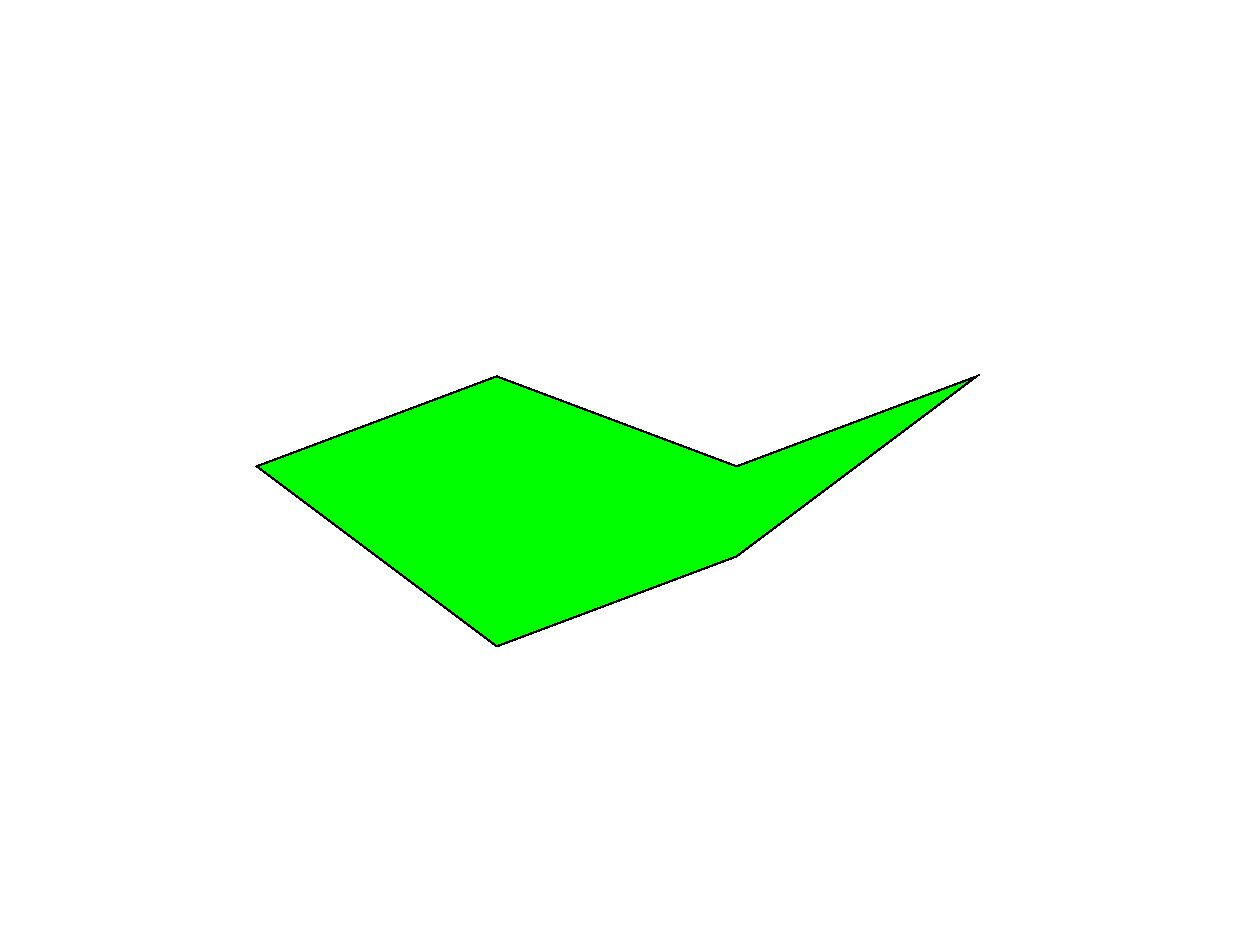
\includegraphics[width=\linewidth]{ch3-shape03.eps}
\caption{Random polygon.}
\label{fig:ch3-shape03}
\end{marginfigure}

Try designing/playing about with different shapes. Perhaps sketch them out on paper first and list down the coordinates before telling \textbf{MATLAB}.

\vspace{1mm}
\noindent\rule{4cm}{0.5pt}
\vspace{2mm}

\noindent If you have the \textbf{MATLAB} \textsf{Image Processing Toolbox}, then you can use the command \texttt{viscircles} to draw circles.

A crude alternative, is to \texttt{scatter} plot a single point ((x,y) location), and set a large size value for the circle. For example:
\begin{docspec}
>> scatter(50,50,1000);
\end{docspec}
or filled:
\begin{docspec}
>> scatter(50,50,1000,'filled');
\end{docspec}

%------------------------------------------------

\subsection{Colors}

You are already familiar with setting colors for lines, with the notation: \texttt{'r'}, or \texttt{'b'} (for red, blue, respectively). This is nice and simple and so totally fabulous ... except there are a limited number of colors available in this notation (see Box).

\marginnote[-1.5in]{\begin{mdframed}[backgroundcolor=gray!10, roundcorner=10pt,leftmargin=1, rightmargin=1, innerleftmargin=5, innerrightmargin=5, innertopmargin=5,innerbottommargin=5, outerlinewidth=1, linecolor=light-gray]
\textbf{MATLAB} quick colors:
\begin{itemize}[noitemsep]
\setlength{\itemindent}{.2in}
\item \texttt{y} -- yellow
\item \texttt{m} -- magenta
\item \texttt{c} -- cyan
\item \texttt{r} -- red
\item \texttt{g} -- green
\item \texttt{b} -- blue
\item \texttt{w} -- white
\item \texttt{k} -- black
\end{itemize}
\end{mdframed}}

Hence there is an alternative that enables a more exact specification of color. In this particular scheme -- red-green-blue, abbreviated to \textit{RGB}, you set the intensity of red, green, and blue, on a scale of 0 to 1. And supply this in a vector format to \textbf{MATLAB}. For example:

\begin{itemize}[noitemsep]
\setlength{\itemindent}{.2in}
\item \texttt{[0 0 0]} -- zero intensity of all of R, G, B => black.
\item \texttt{[1 1 1]} -- 100\% intensity of all of R, G, B => white.
\item \texttt{[1 0 0]} -- 100\% intensity R, none for G and B => red.
\item \texttt{[0.5 0.5 0.5]} -- 50\% intensity of all of R, G, B => grey.
\item \texttt{[0.5 1.0 0.5]} -- light green.
\end{itemize}

Play around with some RGB value combinations, plotting shapes, or filled circles, e.g.
\begin{docspec}
>> scatter(50,50,1000,[0.25 0.75 0.25],'filled');
\end{docspec}

A rendition of the RGB color scale is shown for reference in Figure \ref{fig:RGB_color_solid_cube}. 
\begin{marginfigure}[-4.0in]
\includegraphics[width=\linewidth]{RGB_color_solid_cube.png}
\caption{RGB scale. By SharkD - Own work, GFDL, https://commons.wikimedia.org/
w/index.php?curid=3375025}
\label{fig:RGB_color_solid_cube}
\end{marginfigure}

%------------------------------------------------

\subsection{Creating color maps}

As mentioned earlier -- \textbf{MATLAB} enables a range of different color scales (\textit{colormaps}) to be used in (esp. contour) plotting and provides around  dozen built-in possibilities (see Box).

\marginnote[-2.0in]{\begin{mdframed}[backgroundcolor=gray!10, roundcorner=10pt,leftmargin=1, rightmargin=1, innerleftmargin=5, innerrightmargin=5, innertopmargin=5,innerbottommargin=5, outerlinewidth=1, linecolor=light-gray]
\docenvdef{colormap} (2)
\\ As mentioned earlier, \textbf{MATLAB} has a number of 'colormaps' built in, which are:

\begin{itemize}[noitemsep]
\item parula (default)
\item jet (old default ... avoid ...!)
\item hsv
\item hot    
\item cool
\item spring
\item summer
\item autumn
\item winter
\item gray
\item bone
\item copper
\item pink
\item lines
\item colorcube
\item prism
\item flag
\end{itemize}

\noindent and which you can set by:
\begin{docspecmargin}
>> colormap NAME
\end{docspecmargin}
\noindent (or \texttt{colormap(NAME)}), e.g.:
\begin{docspecmargin}
>> colormap 'hot'
\end{docspecmargin}
\noindent (or \texttt{colormap('hot')})

\end{mdframed}}

Taking the earlier example of loading and plotting the global topography data:

\begin{docspec}
>> data = load('etopo1deg.dat','-ascii');\\
>> imagesc(data);
\end{docspec}

\noindent gives Figure \ref{fig:ch3-etopo3}, and

\begin{docspec}
>> colormap('hot');\\
>> imagesc(data);
\end{docspec}

\noindent gives Figure \ref{fig:ch3-etopo3}.

\begin{marginfigure}[0.0in]
\includegraphics[width=\linewidth]{ch3-etopo3.eps}
\caption{Global topography plotted with the default \textbf{MALTAB} color scheme.}
\label{fig:ch3-etopo3}
\end{marginfigure}

\begin{marginfigure}[0.0in]
\includegraphics[width=\linewidth]{ch3-etopo4.eps}
\caption{Global topography plotted with \texttt{hot}.}
\label{fig:ch3-etopo4}
\end{marginfigure}

You can also define your own \textit{colormap}. \textit{Colormaps} are simply a matrix of \([R G B]\) colors. The most trivial \textit{colormap} would be:

\begin{docspec}
>> cmap1 = [0 0 0];\\
>> colormap(cmap1);
\end{docspec}

\noindent creates and applies a \textit{colormap} containing a single color (black). Try it ... but ti is clearly not very useful ...

Better, would be:

\begin{docspec}
>> cmap2 = [0 0 0; 1 1 1];\\
>> colormap(cmap2);
\end{docspec}

\noindent which creates and applies a color scale containing 2 colors - black and white and when used for the topography data, gives Figure \ref{fig:ch3-etopo5}. 
\sidenote{Remember, \texttt{imagesc} plots using the maximum number of colors available, and in this example, the mid value between the deepest place in the ocean and highest point on land, divides the colors into black and white -- within specifying a particular scale, this color separation does not occur at zero (sealevel)}

\begin{marginfigure}[0.0in]
\includegraphics[width=\linewidth]{ch3-etopo5.eps}
\caption{Global topography plotted with a basic black+white dual color scheme.}
\label{fig:ch3-etopo5}
\end{marginfigure}

You can keep adding colors, e.g.

\begin{docspec}
>> cmap3 = [0 0 0; 0.5 0.5 0.0; 0.0 0.5 0.5; 1 1 1];
\end{docspec}

\noindent but this is a lot of effort to keep adding single additional colors. What you really want to do, is to define end-member colors, and then tell \textbf{MATLAB} to \textit{interpolate} in between these. Recalling back a couple of subsections:

\begin{docspec}
>> ynew = interp1(xold,yold,xnew);
\end{docspec}

\noindent takes the y-values (\texttt{yold}) at x-values \texttt{xold}, and interpolates onto the x-values   defined by the vector \texttt{xnew} (and assigns the new y-values to vector \texttt{ynew}). For instance, if we have the following crudely spaced data\sidenote{In MATLAB notation:
\begin{docspecmargin}
xold = [0 3 7 13 16 22 30];\\
yold = [0.2 0.6 0.7 0.3 0.3 0.1 0.0];
\end{docspecmargin}
}:

\vspace{2mm}
\(\begin{pmatrix}
0 & 0.2 \\
3 & 0.6 \\
7 & 0.7 \\
13 & 0.3 \\
16 & 0.3 \\
22 & 0.1 \\
30 & 0.0 \\
\end{pmatrix}\)
\vspace{2mm}

\noindent and we wanted to create an interpolated dataset from \(0.0\) to \(30.0\) (in x-axis values) in steps of \(1.0\), we would first create the new x-axis vector that the data will be interpolated on to:

\begin{docspec}
xnew = [0.0:1.0:30.0];
\end{docspec}

\noindent and then we would write:

\begin{docspec}
>> ynew = interp1(xold,yold,xnew,'spline');
\end{docspec}

\noindent and obtain the interpolated data as shown in Figure \ref{fig:ch3-interp1}. (Try this.)

\begin{marginfigure}[0.75in]
\includegraphics[width=\linewidth]{ch3-interp1.eps}
\caption{Comparison of sparsely sampled data (points) compared with a more finely spaced spline interpolation (solid line). (x-axis and y-axis are both unit-less.)}
\label{fig:ch3-interp1}
\end{marginfigure}

We can do something similar for the \textit{colormaps}. Consider the simple end-member black-to-white white scale:

\begin{docspec}
>> cmap2 = [0 0 0; 1 1 1];
\end{docspec}

\noindent We can write this as points along a vector \(x\) (the axis not representing anything in particular -- the number of the color, or simply the normalized distance between the extreme end-member colors), together 3 color vectors (for the separate red, green, and blue  component values):

\vspace{2mm}
\(xold = \begin{pmatrix}0.0 \\
1.0 \\
\end{pmatrix}\),
\(rold = \begin{pmatrix}0.0 \\
1.0 \\
\end{pmatrix}\),
\(gold = \begin{pmatrix}0.0 \\
1.0 \\
\end{pmatrix}\),
\(bold = \begin{pmatrix}0.0 \\
1.0 \\
\end{pmatrix}\)
\vspace{2mm}

\noindent and:

\begin{docspec}
>> xold = [0.0; 1.0];\\
>> rold = [0; 1];\\
>> gold = [0; 1];\\
>> bold = [0; 1];
\end{docspec}

If we want to create a scale of 11 total (from \(0.0\) to \(1.0\) in steps of \(0.1\)) different colors, we can create a new \(x\) vector to interpolate on to:

\begin{docspec}
xnew = [0.0:0.1:1.0];
\end{docspec}

\noindent and then either interpolate the 3 color vectors separately:

\begin{docspec}
rnew = interp1(xold,rold,xnew,'spline');\\
gnew = interp1(xold,gold,xnew,'spline');\\
bnew = interp1(xold,bold,xnew,'spline');
\end{docspec}

\noindent or \textbf{MATLAB} allows us to interpolate all together if we first combine the sperate vectors:

\begin{docspec}
mapold = [rold gold bold];
\end{docspec}

\noindent and then:

\begin{docspec}
mapnew = interp1(xold,mapold,xnew,'spline');
\end{docspec}

If you now set the new \textit{colormap} (\texttt{>> colormap(mapnew);}) and re-plot the global topography, you should get Figure \ref{fig:ch3-etopo6}.

\begin{marginfigure}[0.0in]
\includegraphics[width=\linewidth]{ch3-etopo6.eps}
\caption{Global topography plotted with a user-defined grey-scale.}
\label{fig:ch3-etopo6}
\end{marginfigure}

%------------------------------------------------

\subsection{Placing and making text nice}

There is not much to placing text and specifying its properties. The \textbf{MATLAB} command for writing a string to a \textsf{figure window}, is \docenvdef{text}. That's it! (see Boxes)

For instance, you could write:

\begin{docspec}
>> text(25,25,'bananas');
\end{docspec}

\noindent and the text \texttt{bananas} will appear at location \((25,25)\) on your plot.

Additional parameters can be added to change font, size, etc (see Box), e.g.:

\begin{docspec}
>> text(25,25,'bananas','FontSize',24,'Color',[0 1 1]);
\end{docspec}

\noindent for big light blue bananas.

\marginnote[-1.5in]{\begin{mdframed}[backgroundcolor=light-gray, roundcorner=10pt,leftmargin=1, rightmargin=1, innerleftmargin=5, innerrightmargin=5, innertopmargin=5,innerbottommargin=5, outerlinewidth=1, linecolor=light-gray]
\docenvdef{text}
\begin{docspecmargin}
text(X,Y,STRING);
\end{docspecmargin}
will write the string contained in the variable STRING (or you can pass the text as a string directly), at location (X,Y).
\\Note that by default, MATLAB alights the left-hand edge of the text with the X coordinate position, and the mid-point of the string vertically, with the Y coordinate. i.e. the string is \textit{left-aligned} and \textit{centered} vertically.
\\A variety of additional properties can be set at the time, e.g.
\vspace{-4mm}
\begin{docspecmargin}
text(X,Y,STRING,'FontSize',12);
\end{docspecmargin}
specifies a 12 pt font size. Other common parameter options include:
\begin{itemize}[noitemsep]
\setlength{\itemindent}{.2in}
\item \texttt{'FontName'}
\item \texttt{'Color'}
\item \texttt{'Rotation'}
\item \texttt{'HorizontalAlignment'}
\item \texttt{'VerticalAlignment'}
\end{itemize}
See \textbf{MATLAB} \texttt{help} for more details.
\end{mdframed}}

\marginnote{\begin{mdframed}[backgroundcolor=light-gray, roundcorner=10pt,leftmargin=1, rightmargin=1, innerleftmargin=5, innerrightmargin=5, innertopmargin=5,innerbottommargin=5, outerlinewidth=1, linecolor=light-gray]
When \textbf{MATLAB} displays text, be aware that there are a bunch of special characters that may not come out as the character you want. The more common ones are:
\\ \texttt{\_} -- will make the following character a subscript, or a sequence of characters if you place them within a pair of curly brackets \{\}.
\\ \texttt{\(\wedge\)} -- will make the following character a subscript, or a sequence of characters if you place them within a pair of curly brackets \{\}.
\end{mdframed}}

%----------------------------------------------------------------------------------------

%----------------------------------------------------------------------------------------
% CHAPTER 4
%----------------------------------------------------------------------------------------

\chapter{Further ... Programming}
\label{ch:04}

%------------------------------------------------

In this chapter we'll get some (more) practice building programs and crafting (often) bite-sized chunks of code that solve a specific, normally computational or numerical (rather than scientific) problem (\textit{algorithms})
\sidenote[][-0.75in]{According to the all-mighty Wikipdeia (and who am I to argue?) -- an "\textit{algorithm ... is a self-contained step-by-step set of operations to be performed. Algorithms perform calculation, data processing, and/or automated reasoning tasks.}"}.

\marginnote[-0.0in]{\begin{mdframed}[backgroundcolor=light-blue, roundcorner=10pt,leftmargin=1, rightmargin=1, innerleftmargin=5, innerrightmargin=5, innertopmargin=5,innerbottommargin=5, outerlinewidth=1, linecolor=gray!10]
\textbf{Search algorithms}
\\Lets assume that you have a function:
\\\(y=f(x)\)
\\\noindent There are two common cases that you might want to solve (or approximate):
\begin{enumerate}[noitemsep]
\setlength{\itemindent}{.2in}
\item The value of \(x\) such that the value of \(f(x)\) is minimized (\(y\simeq0\)).
\item The value of \(x\) such that the value of \(\frac{dy}{dx}\) is minimized (first derivative \(\simeq0\).
\end{enumerate}
Lets further assume that you can place some initial limits on \(x: x_{min}\leq x \leq x_{max}\).
\\A good place to start in both examples is to test the mid-point of the limits: \(f(\frac{x_{min}+x_{max}}{2})\) (In some cases you might instead take the log-weighted mean.)
\\In case \#1 and assuming that \(\frac{dy}{dx}\) is positive, if:
\\\(f(\frac{x_{min}+x_{max}}{2})>0\)
\\\noindent you replace \(x_{max}\) with \(\frac{x_{min}+x_{max}}{2}\) (the current tested value of \(x\)) and if: 
\\\(f(\frac{x_{min}+x_{max}}{2}) < 0\)
\\\noindent you replace \(x_{min}\) with \(\frac{x_{min}+x_{max}}{2}\). Keep repeating until the difference \(y\) and zero falls beneath some specified tolerance.
\\In case \#2, you need to test the value of \(f(x)\) infinitesimally away from \(f(\frac{x_{min}+x_{max}}{2})\) to determine whether the gradient is positive or negative (assuming that you do not \textit{a priori} know the derivative function). The idea here is to ensure that the values of \(x_{min}\) and \(x_{max}\) correspond to positive and negative (or negative and positive) gradients. i.e. \(\frac{x_{min}+x_{max}}{2}\) replaces \(x_{min}\) or \(x_{max}\) according to which has the same sign of gradient.
\end{mdframed}}

%------------------------------------------------

\newpage

%------------------------------------------------

\section{Nested loops}

A helpful device, particularly when dealing with arrays of data in \textbf{MATLAB}, is to \textit{nest} loops -- i.e place one loop inside another one. (So far, you have seen single loops, and single loops with conditions inside, but not nested loops.) A generic code for a nested loop might look like:
\begin{docspec}
\textcolor[rgb]{0,0.501961,0}{\% loop 1 start\\}
\textcolor{blue}{for} n=1:10\\
\ \ \ \textcolor[rgb]{0,0.501961,0}{\% loop 2 start\\}
\ \ \ \textcolor{blue}{for} m=1:10\\
\ \ \ \ \ \ \textcolor[rgb]{0,0.501961,0}{\% CODE\\}
\ \ \ \textcolor{blue}{end}\\
\textcolor{blue}{end}
\end{docspec}
Here, the value of \texttt{n} cycles (loops) from \(1\) to \(10\) (i.e. the loop goes around 10 times). Then ... for each value of \texttt{n}, the value of \texttt{m} also cycles from \(1\) to \(10\). The code in the middle of the innermost loop is then executed a total of \(10\times 10=100\) times.

Why would you do this? An Example.

Image you are programming a game of Tic-tac-toe (in fact we will, in a later chapter!). The drawn grid might look like Figure \ref{fig:ch6-grid1}.\sidenote[][-2.5in]{In this case, player \textsf{x} has obviously already won. What was \textsf{naughts} thinking???}

\begin{marginfigure}[-2.0in]
\includegraphics[width=\linewidth]{ch6-grid1.eps}
\caption{Tic-tac-toe game grid.}
\label{fig:ch6-grid1}
\end{marginfigure}

In terms of \textbf{MATLAB} and computer programming, we might create a representation of the grid, and assign \texttt{0} to unpicked squares, a \texttt{1} for where a cross is, and a \texttt{2} for where a naught is, as per Figure \ref{fig:ch6-grid2} (because we cannot numerically represent an actual cross or circle shape). 
\begin{marginfigure}[0.0in]
\includegraphics[width=\linewidth]{ch6-grid2.eps}
\caption{Tic-tac-toe game grid with numerical codes overlain.}
\label{fig:ch6-grid2}
\end{marginfigure}

To store this information, we could create an array in which each location would have a value of \texttt{0}, \texttt{1}, or \texttt{2}, e.g.

\vspace{2mm}
\(\begin{pmatrix}1 & 2 & 0 \\
1 & 2 & 0 \\
1 & 0 & 0 \\
\end{pmatrix}\)
\vspace{2mm}

\noindent and as per Figure \ref{fig:ch6-grid3}

\begin{marginfigure}[0.0in]
\includegraphics[width=\linewidth]{ch6-grid3.eps}
\caption{Tic-tac-toe game grid -- numerical representation.}
\label{fig:ch6-grid3}
\end{marginfigure}

OK -- ignore the existence of the \textbf{MATLAB} \textit{function} find, and lets say that you want find the locations of the crosses -- '\texttt{1}'s in the array code notation. You need to test each an every location in the array (lets call it \texttt{tokens}) in turn for whether its contents is a '\texttt{1}' or not. We could do this long-hand ...
\begin{docspec}
\textcolor{blue}{if} ( (tokens(1,1) == 1) || (tokens(2,1) == 1) ||\\
\ \ \ (tokens(3,1) == 1) || (tokens(1,2) == 1) || ...
\end{docspec}
... and would get desperately tedious pretty quickly. And what if the grid (array) was \(100\times 100\)? You could have to have \(10,000\) tests of an equality in the \texttt{\textcolor{blue}{if}} ...

The idea then is to loop through all the locations in the array. And we do this by: For each row (in a loop), loop through all the columns. Our code fragment would then loop like:
\begin{docspec}
\textcolor[rgb]{0,0.501961,0}{\% loop 1 start\\}
\textcolor{blue}{for} row=1:3\\
\ \ \ \textcolor[rgb]{0,0.501961,0}{\% loop 2 start\\}
\ \ \ \textcolor{blue}{for} column=1:3\\
\ \ \ \ \ \ \textcolor{blue}{if} (tokens(row,column) == 1),\\
\ \ \ \ \ \ \ \ \ ...\\
\ \ \ \textcolor{blue}{end}\\
\textcolor{blue}{end}
\end{docspec}
and hence you thereby visit each and every array location in turn -- working across every column, for each and every row, as per Figure \ref{fig:ch6-grid4}.

\begin{marginfigure}[0.0in]
\includegraphics[width=\linewidth]{ch6-grid4.eps}
\caption{Tic-tac-toe game grid -- search order: columns then rows.}
\label{fig:ch6-grid4}
\end{marginfigure}

We could also carry out the search in the opposite order:
\begin{docspec}
\textcolor[rgb]{0,0.501961,0}{\% loop 1 start\\}
\textcolor{blue}{for} column=1:3\\
\ \ \ \textcolor[rgb]{0,0.501961,0}{\% loop 2 start\\}
\ \ \ \textcolor{blue}{for} row=1:3\\
\ \ \ \ \ \ \textcolor{blue}{if} (tokens(row,column) == 1),\\
\ \ \ \ \ \ \ \ \ ...\\
\ \ \ \textcolor{blue}{end}\\
\textcolor{blue}{end}
\end{docspec}
(Figure \ref{fig:ch6-grid5}) Then result would be exactly the same. TO some extend, which axis direction you choose as the outer loop, is a matter of personal preference\sidenote{When arrays are small, the the overall computational expense small.}.

\begin{marginfigure}[0.0in]
\includegraphics[width=\linewidth]{ch6-grid5.eps}
\caption{Tic-tac-toe game grid -- search order: rows then columns.}
\label{fig:ch6-grid5}
\end{marginfigure}

You can also search in the opposite directions, e.g.
\begin{docspec}
\textcolor[rgb]{0,0.501961,0}{\% loop 1 start\\}
\textcolor{blue}{for} column=1:3\\
\ \ \ \textcolor[rgb]{0,0.501961,0}{\% loop 2 start\\}
\ \ \ \textcolor{blue}{for} row=3:-1:1\\
\ \ \ \ \ \ \textcolor{blue}{if} (tokens(row,column) == 1),\\
\ \ \ \ \ \ \ \ \ ...\\
\ \ \ \textcolor{blue}{end}\\
\textcolor{blue}{end}
\end{docspec}
searches across columns, form left-to-right, but rows in the order bottom-to-top. This perhaps looks a little like how you might visualize a search on a \textit{(lon,lat)} grid(?)

The concept is the same even for very large grids (where you cannot easily draw a graphical representation to help you).

Nor, do the number of rows and columns have to be the same. For example you might want to access information stored in an array that has a cell location for every day of the year. In this case, you might have 12 columns for the 12 months, and 31 rows so that you can accommodate the number of days in the longest month.\sidenote{MATLAB does not allow the number of rows to differ, from column to column -- a matrix must have a strictly rectangular shape. \textbf{MATLAB} and other programming languages allow the creation of \textit{objects}, that are more flexible.} In fact, in this example, the inner loop -- days -- might have a different loop maximum, depending on which month, e.g.
\begin{docspec}
\textcolor[rgb]{0,0.501961,0}{\% month loop start\\}
\textcolor{blue}{for} month=1:12\\
\ \ \ \textcolor[rgb]{0,0.501961,0}{\% determine length of month\\}
\ \ \ \textcolor{blue}{switch} month\\
\ \ \ \ \ \     \textcolor{blue}{case} {1, 3, 5, 7, 8, 10, 12}\\
\ \ \ \ \ \ \ \ \         day\_max = 31;\\
\ \ \ \ \ \     \textcolor{blue}{case} {4, 6, 9, 11}\\
\ \ \ \ \ \ \ \ \         day\_max = 30;\\
\ \ \ \ \ \     \textcolor{blue}{case} {2}\\
\ \ \ \ \ \ \ \ \         day\_max = 29;\\
\ \ \ \textcolor{blue}{end}\\
\ \ \ \textcolor[rgb]{0,0.501961,0}{\% day loop start\\}
\ \ \ \textcolor{blue}{for} day=1:day\_max\\
\ \ \ \ \ \ \textcolor[rgb]{0,0.501961,0}{\% CODE\\}
\ \ \ \textcolor{blue}{end}\\
\textcolor{blue}{end}
\end{docspec}

\vspace{1mm}
\noindent\rule{4cm}{0.5pt}
\vspace{-2mm}

\newthought{To test your understanding ...} for the matrix:

\vspace{4mm}
\(A=\begin{pmatrix}4 & 66 & 13 & 42 & 36 & 14 \\
33 & 4 & 0 & 28 & 11 & 22 \\
18 & 26 & 7 & 1 & 5 & 19 \\
12 & 9 & 23 & 30 & 7 & 2 \\
0 & 0 & 2 & 0 & 15 & 33 \\
14 & 42 & 17 & 27 & 8 & 0 \\
\end{pmatrix}\)
\vspace{4mm}

\noindent determine ... NOT using \texttt{find} (or similar), but rather a nested loop, how many occurrences there are of values
\sidenote{Hint: Before the next loop starts, you'll need to define a parameter to keep count of the number of values you find that meet the criteria, and set it to zero. Then in the (nested) loop, increment the counter variable by \texttt{1} each time you find a value matching the criteria.}
\sidenote{Also hint: At the start of the script (after your initial descriptive comments!), define \texttt{A}.}:

\begin{enumerate}[noitemsep]
\item greater than \texttt{9}
\item greater than \texttt{9} but less than \texttt{20}
\end{enumerate}

Make this a new \textit{script} \textbf{m-file} program. Display (\texttt{disp}) the result at the end (after the (nested) loop has ended).

\vspace{1mm}
\noindent\rule{4cm}{0.5pt}
\vspace{-2mm}

\newthought{Next}: for the simple tic-tac-toe (\(3\times3\)) grid, at each (\textit{column,row}) location, you are going to draw a colored square.

Firstly, at the start of a new \textit{script} \textbf{m-file}, add:

\begin{docspec}
\textcolor[rgb]{0,0.501961,0}{\% **************************\\
\% YOUR COMMENTS ON WHAT THE PROGRAM DOES\\
\% **************************\\}
\ \\
\textcolor[rgb]{0,0.501961,0}{\% create a new figure window\\}
figure;\\
\textcolor[rgb]{0,0.501961,0}{\% create a set of invisible axes that will the window\\}
fh = axes(\textcolor[rgb]{1,0,1}{'Position'},[0 0 1 1],\textcolor[rgb]{1,0,1}{'Visible'},\textcolor[rgb]{1,0,1}{'off'});\\
\textcolor[rgb]{0,0.501961,0}{\% scale the axes\\}
axis([0 3 0 3]);\\
\textcolor[rgb]{0,0.501961,0}{\% hold on!\\}
hold \textcolor[rgb]{1,0,1}{on};
\end{docspec}

\noindent Here:

\begin{itemize}[noitemsep]
\item The line starting \texttt{fh = ...} creates a plotting area with no axes visible, and filling the Figure window area (\texttt{[0 0 1 1]} in normalized units). The handle to this is returned (variable \texttt{fh}), just in case we ever need it later.
\item Then, the axes are scaled for convenience -- there are 3 rows and 3 columns in the grid we want to create, so a 'reasonable' choice is to set \texttt{axis([0 3 0 3])}, although we need not have.
\item You know what \texttt{hold on} does, right ... ?
\end{itemize}

You can then add (after) the nested loop code framework:

\begin{docspec}
\textcolor[rgb]{0,0.501961,0}{\% loop 1 start\\}
\textcolor{blue}{for} column=1:3\\
\ \ \ \textcolor[rgb]{0,0.501961,0}{\% loop 2 start\\}
\ \ \ \textcolor{blue}{for} row=1:3\\
\ \ \ \ \ \ \ \ \ ...\\
\ \ \ \textcolor{blue}{end}\\
\textcolor{blue}{end}
\end{docspec}

To draw a square, the easiest function to use is \texttt{patch} (see earlier). For the coordinate parameters to be passed to \texttt{patch}, if your current location in the loop is \texttt{column=1}, \texttt{row=1} -- now taking for convenience, a notation and orientation where we start counting from the \uline{bottom left-hand corner} (unlike in the previous notation and orientation) --  the coordinates for the square are:
\vspace{1mm}
\\\((0,0), (1,0), (1,1), (0,1)\)
\vspace{1mm}
\\\noindent and for which \texttt{patch} will take input:

\begin{docspec}
patch([0 1 1 0], [0 0 1 1],'black');
\end{docspec}

\noindent (remembering that patch takes a vector of all the \textit{x}-coordinates as a 1st parameter, and then a vector of all the \textit{y}-coordinates as the second parameter)

If you do not more than this, you end up looping through the (\(3\times3\)) grid, but only even (re-)plotting the same square in the bottom left-hand corner ...

The mental leap is to \uline{generalize} the problem and  to notice that if your column (\textit{x}) and row (\textit{y}) values are held in variables \texttt{column} and \texttt{row}, respectively, you could write:

\begin{docspec}
patch([column-1 column column column-1], ...\\
\ \ \ [row-1 row-1 row row],'black');
\end{docspec}

Complete the code and try this. You should end up with 9 black squares in a (\(3\times3\)) grid ... which will simply look like a huge black square filling the figure window, as per Figure \ref{fig:ch4-grid1} ... :o)

\begin{marginfigure}[0.0in]
\includegraphics[width=\linewidth]{ch4-grid1.eps}
\caption{3x3 grid of black squares ...}
\label{fig:ch4-grid1}
\end{marginfigure}

You could make it a little more interesting by creating a color value derived from the values of the \texttt{column} and \texttt{row} counters. e.g. if you write:

\begin{docspec}
patch([column-1 column column column-1], ...\\
\ \ \ [row-1 row-1 row row],color);
\end{docspec}

\noindent (substituting a specification of \texttt{'black'} for whatever color corresponds to the value contained in variable \texttt{color}), and immediately before this (still in the loop) write:

\begin{docspec}
color = (column + row);
\end{docspec}

Re-running the script, you now get Figure \ref{fig:ch4-grid2}.

\begin{marginfigure}[0.0in]
\includegraphics[width=\linewidth]{ch4-grid2.eps}
\caption{3x3 grid of colored squares.}
\label{fig:ch4-grid2}
\end{marginfigure}

You might notice that the colors are the same along diagonals, because you get the same value of \texttt{color} whether you are at location \((1,2)\) or \((2,1)\). We could make the location colors more distinct by modifying how we derive a value for \texttt{color}, e.g.

\begin{docspec}
color = (column\(^{\wedge}\)2 + row);
\end{docspec}

\noindent (Figure \ref{fig:ch4-grid3})

\begin{marginfigure}[0.0in]
\includegraphics[width=\linewidth]{ch4-grid3.eps}
\caption{(yawn)}
\label{fig:ch4-grid3}
\end{marginfigure}

Maybe play about a little creating different patterns of colors by means of different equations combining the values of \texttt{column} and \texttt{row}.

\vspace{1mm}
\noindent\rule{4cm}{0.5pt}
\vspace{-2mm}

\newthought{As a final example, consider teh chess board.} A chess board consists of squares in a \(8\times8\) grid. The squares alternate black and white. To define 8 squares (points) along the \textit{x}-axis on the bottom row, you'd write something of the form:
\begin{docspec}
\textcolor{blue}{for} m=1:8
\\ \ \ \ \textcolor[rgb]{0,0.501961,0}{\% SOME CODE GOES HERE}
\\\textcolor{blue}{end}
\end{docspec}
Now, if you wanted to define 8 squares along each column (the \textit{y}-axis), at each and every \textit{x}-axis value, you'd need to loop through all the rows, So you need a loop in e.g. \texttt{n}, inside the loop for \texttt{m}:
\begin{docspec}
\textcolor{blue}{for} m=1:8
\\ \ \ \ \textcolor{blue}{for} n=1:8
\\ \ \ \ \ \ \ \textcolor[rgb]{0,0.501961,0}{\% SOME CODE GOES HERE}
\\ \ \ \ \textcolor{blue}{end}
\\\textcolor{blue}{end}
\end{docspec}
Follow this through to satisfy yourself that for each and every value of \texttt{m} from \texttt{1} to \texttt{8}, \texttt{n} loops from \texttt{1} to \texttt{8}, and hence visits every point in turn of a  \(8\times8\) (\texttt{n,m}) grid.

Actually, now we have got this far, it is good practice to consider how we'd define the black and white squares. We'll assume that black is represented by '\texttt{1}' (\textit{true}) and white by \texttt{'0'} (\textit{false}) and create a board (array) of all white squares to start with, i.e.
\begin{docspec}
board = zeros(8);
\end{docspec}
\noindent(Refer to \textbf{help} or earlier for the syntax for help on the function \texttt{zeros}.\sidenote[][-1.5in]{You could alternatively write this:
\begin{docspecmargin}board = zeros(8,8);\end{docspecmargin}})

\marginnote[-1.0in]{\begin{mdframed}[backgroundcolor=gray!10, roundcorner=10pt,leftmargin=1, rightmargin=1, innerleftmargin=5, innerrightmargin=5, innertopmargin=5,innerbottommargin=5, outerlinewidth=1, linecolor=light-gray]
\docenvdef{mod}
\\Not ... the opposite of \docenvdef{rocker} (which doesn't exist in \textbf{MATLAB} anyway) but short for \textit{modulo}. Wikipedia helpfully tells us:
\\"\textit{In computing, the modulo operation finds the remainder after division of one number by another (sometimes called modulus).}"
\\Or in \textbf{MATLAB}-speak:
\begin{docspecmargin}
b = mod(a,m) 
\end{docspecmargin}
"\textit{returns the remainder after division of \texttt{a} by \texttt{m}, where \texttt{a} is the dividend and \texttt{m} is the divisor}".
\\It turns out that as long as a is positive, you can use to test for whether an integer \texttt{a} is \textit{even} or \textit{odd} by:
\begin{docspecmargin}
b = mod(a,2) 
\end{docspecmargin}
When the returned value \texttt{b} is \texttt{0}, \texttt{a} is \textit{even}, and when \texttt{b} is \texttt{1}, \texttt{a} is \textit{odd}.
\end{mdframed}}

If we start with a black square ('\texttt{1}') at the bottom left, we could define an \textit{algorithm} for creating the grid as: odd column number squares are black, as long as the row number is odd, otherwise they are white.\sidenote{Look up a picture of a chess board to convince yourself that this works.} So to implement this in code -- as we loop through both column (\texttt{m}) and row (\texttt{n}) on the board, we test for  the column number being odd and row number odd, OR, the column number being even and row number being even. If \textit{true}, the square is defined as black. The only tricky bit is to determine whether the row or column number is even or odd. We do this by testing whether there is any remainder after dividing by 2, using the function \docenv{mod}.

The complete code looks like:
\begin{docspecmargin}
board = zeros(8);
\\\textcolor{blue}{for} m=1:8
\\ \ \ \ \ \textcolor{blue}{for} n=1:8
\\ \ \ \ \ \ \ \ \ \textcolor{blue}{if} ((mod(m,2)>0 \&\& mod(n,2)>0) || (mod(m,2)==0 \&\& mod(n,2)==0))
\\ \ \ \ \ \ \ \ \ \ \ \ \ board(n,m) = 1;
\\ \ \ \ \ \ \ \ \ \textcolor{blue}{end}
\\ \ \ \ \ \textcolor{blue}{end}
\\\textcolor{blue}{end}
\end{docspecmargin}
Spend a little time decoding the \texttt{if} statement for practice ...
If you want to see that it works -- code it in a new \textbf{m-file}, run it, and then plot up \texttt{board} by e.g. using \texttt{imagesc} (cf. Figure \ref{fig:ch8-chess}). Beautiful.

\begin{marginfigure}[0.0in]
\includegraphics[width=\linewidth]{ch8-chess.png}
\caption{Chess board grid pattern.}
\label{fig:ch8-chess}
\end{marginfigure}


%------------------------------------------------

\newpage

%------------------------------------------------

\section{Algorithms and problem-solving}

This (algorithms  and problem-solving) is not something that can really be 'taught' \textit{per se}, but rather practised and aided by a logical state of mind. We'll go through a series of step-by-step examples. Hopefully this will also illustrate some general coding approaches.

%------------------------------------------------

\subsection{Example \#1: max(!)}

So yes, this is a built-in \textit{function} \texttt{max} in \textbf{MATLAB}, but suspend disbelief for a moment ... and pretend that there is not one. What if we wanted to create one, i.e. \textit{function} that is passed a vector of numbers, and returns the maximum value?

So already, from the definition of the problem, you know to create a new \textbf{m-file} a define a \textit{function}, that takes as input a variable (a vector), and returns the largest value in that vector.\sidenote{Note that you do not need to specify that the input variable is a vector, just that there is a variable input.}\sidenote{Here, my personal naming convention has:\\
\texttt{s\_out} -- the output variable, and \texttt{s} for scalar\\
\texttt{v\_in} -- an input variable, with \texttt{v} designating vector ...\\(This is perhaps, overkill, but leads little room for any confusion later.)}

\begin{docspec}
\textcolor{blue}{function} [s\_out] = maxxx(v\_in)\\
\textcolor[rgb]{0,0.501961,0}{\% maxxx\\
\%\\
\% Takes a (single) vector as input, returns the maximum value.}\\
\ \\
\textcolor{blue}{end}
\end{docspec}

You have hence created a (empty) shell for the program. You could try calling it/running it at the command line ... to check there is no problem so far, although it is clearly not going to do anything. You could extend your basic testing by returning just the first element of the input vector, i.e., before \texttt{end}, add:

\begin{docspec}
s\_out = v\_in(1);
\end{docspec}

You are still not solving the problem, but in this step, you have now demonstrated that your function can take in a (vector) input, do something with it, and set the output variable (/return a scalar output)\marginnote{Which in this example just happens to be the first element of the vector}.

OK, so ... we need to devise an algorithm to find the largest value in the vector \texttt{v\_in}. The first piece of potentially useful information you can find, is the number of elements in the vector. You can obtain this via the function \docenv{length}\sidenote{It turns out that \texttt{length} does not care about the orientation of a vector, and:
\begin{docspecmargin}
A=[1:10];\\
length(A)
\end{docspecmargin}
gives the same answer (\texttt{10}) as:
\begin{docspecmargin}
A=[1:10]';\\
length(A)
\end{docspecmargin}}.

So at the top of the function (below the comment lines), you could create a variable, set equal to the number of elements in the vector that you are going to have to process:

\begin{docspec}
nmax = length(v\_in);
\end{docspec}

What about the next part or structure in the program? You are going to need to look through all the elements of the vector if you are going to find the maximum value, so presumably a loop is required -- one that goes from the first to last element of the vector:

\begin{docspec}
\textcolor{blue}{for} n = 1:nmax,\\
\ \\
\textcolor{blue}{end}
\end{docspec}

The crux of the problem is recognising that you need to keep a running maximum, or a local or temporary maximum value, that is your maximum value so far, as you progress through repeated iterations of the loop. With this value, you are going to test whether each element of the array is larger than it -- if true (the element in the vector being tested is larger than the current or largest-to-date maximum estimate) -- you are going to replace the current maximum estimate, with the vector element (that you have just found is larger than your largest so far). We could call this variable, e.g. \texttt{temp\_max} to indicate that is it temporary and not necessarily the largest value of the vector as a whole.

\uline{Within the loop}, the test we make is therefore:

\begin{docspec}
\ \ \ \textcolor{blue}{if} (v\_in(n) > temp\_max),\\
\ \ \ \ \ \ temp\_max = v\_in(n);\\
\ \ \ \textcolor{blue}{end}
\end{docspec}

Almost there. Run the program/function and see what happens.

\textbf{MATLAB} is unhappy about the line where the value of \texttt{temp\_max} is being tested against v\_in(n). It may be obvious to you when (in terms of loop iterations) this is occurring. If not, why not, just after:

\begin{docspec}
\textcolor{blue}{for} n = 1:nmax,
\end{docspec} 

\noindent \texttt{disp}(lay) the value of \texttt{n}. OR, add a breakpoint on the problem line, so that \textbf{MATLAB} will pause just before the line that gave the error, is executed.

Either way, you should have found that the value of \texttt{n} is \texttt{1}, i.e. the error is occurring on the very first iteration of the loop. Why? As per the error -- \textbf{MATLAB} does not know what \texttt{temp\_max} is, and this occurs, if you have not yet assigned it a value.

So our problem is one of initialization -- we need to give \texttt{temp\_max} an initial value, so that when the first iteration of the loop occurs, and the first element in the vector is accessed, there is something to compare it with.

There are 2 (probably 99999999) ways to go about this:
 
\begin{enumerate}[noitemsep]
\setlength{\itemindent}{.2in}
\item Seed the value of \texttt{temp\_max} with a value so improbably small, that you are betting that any conceivable array of numbers with have a number greater than this.\sidenote{There are obvious dangers here, should a vector of all insanely low values be given as an input. You could for instance determine whether any of the values were higher than the seed value, and if not, report or return an error message. So in this case, even if the function did not work, you would be told why. A bit like \textbf{MATLAB} functions in general, no?} For example, \uline{before} the loop starts, you might write:
\begin{docspec}
\texttt{temp\_max} = -999999999;
\end{docspec} And then go through testing all \texttt{nmax} elements in the vector.
\item Better, would be to initialize your temporary maximum variable with the fist element in the vector. But then, you need to recognise that you need not test this against the first element, and the loop can start at 2:
\begin{docspec}
\texttt{nmax} = v\_in(1);\\
\textcolor{blue}{for} n = 2:nmax,
\end{docspec} 
\end{enumerate}

Finally, remember to set the output variable equal to the maximum value that you find.\sidenote{After the loop ends.}

The following is the complete working code of the problem\sidenote{Note the liberal use of comments, and also the indentation of the code within the \texttt{for} loop as well as within the \texttt{if} conditional.}:

\begin{docspec}
\textcolor{blue}{function} [s\_out] = maxxx(v\_in)\\
\textcolor[rgb]{0,0.501961,0}{\% maxxx\\
\%\\
\% Takes a (single) vector as input, returns the maximum value.}\\
\ \\

\textcolor[rgb]{0,0.501961,0}{\% Determine number of elements in vector}\\
nmax = length(v\_in);
\textcolor[rgb]{0,0.501961,0}{\% Seed temporary (running maximum) variable}\\
temp\_max = v\_in(1);\\
\textcolor[rgb]{0,0.501961,0}{\% Loop through all but the first element in the vector}\\
\textcolor{blue}{for} n = 2:nmax,\\
\ \ \ \textcolor{blue}{if} (v\_in(n) > temp\_max),\\
\ \ \ \ \ \ temp\_max = v\_in(n);\\
\ \ \ \textcolor{blue}{end}\\
\textcolor{blue}{end}\\
\textcolor[rgb]{0,0.501961,0}{\% Set function (return) value}\\
s\_out = temp\_max;\\
\textcolor{blue}{end}
\end{docspec}

There are 2 further testing or debugging (if you have issues) steps:

\begin{enumerate}[noitemsep]
\setlength{\itemindent}{.2in}
\item Firstly, simply go through in your mind, what you think happens on each iteration. Writing down how the values, e.g. of the temporary variable change on each iteration, is a good idea. Obviously you can do this prior to writing the code, to give you an idea of how it will work (or not).
\item Create a series of test arrays, or varying length, ordered, or random numbers, integers and/or reals, plug them in, and see if your function works each and every time.
\end{enumerate}

\vspace{1mm}
\noindent\rule{4cm}{0.5pt}
\vspace{-2mm}

\newthought{If you are passably happy with that --} write a (new) function that finds the \textit{minimum} element in a vector array.\sidenote[][-1.0in]{This is in fact employed a little later, where it is referred to as \texttt{minxx}.}

\vspace{1mm}
\noindent\rule{4cm}{0.5pt}
\vspace{-2mm}

\newthought{Then ... as a 3rd function --} return a second variable from the function -- equal to the number of elements that are equal maximum.\sidenote[][-1.0in]{If we were cheating, and we \uline{are not} ... then one could use the built-in \textbf{MATLAB} functions as so:
\begin{docspecmargin}length(find(A==max(A)));
\end{docspecmargin}
Which says ... find the elements in A, equal to \texttt{max(A)} and determine the \texttt{length} (number of elements) of this resulting vector (\texttt{find(A==max(A))}) ...} (i.e. if the maximum value appears 5 times in the input vector ... you additionally return the number '\texttt{5}'.)

The structure of the \textit{function} will now look like:
\begin{docspec}
\textcolor{blue}{function} [s\_out1 s\_out2] = maxxxes(v\_in)\\
\textcolor[rgb]{0,0.501961,0}{\% maxxxes\\
\%\\
\% Takes a (single) vector as input, returns the maximum value
\\ and the number of elements equal to that value.}\\
\ \\
\textcolor{blue}{end}
\end{docspec}
which passes back two variables.

The first variable (\texttt{s\_out1}) -- the maximum value of the elements in the input vector, is as before. You need to work out the code to determine the value of \texttt{s\_out2}. The key to this, is recognising that previously, when the value of \texttt{temp\_max} was equal to \texttt{v\_in(n)}, you did nothing, as you were only interested in \texttt{v\_in(n) > temp\_max} and hence updating (replacing) the current value of \texttt{temp\_max}. What you need is an \texttt{elseif} statement, and test whether you have found a second value in the vector equal to \texttt{temp\_max}. If so, you need to somehow record this occurrence.

A partial solution might look like:
\begin{docspec}
\textcolor[rgb]{0,0.501961,0}{\% Loop through all but the first element in the vector}\\
\textcolor{blue}{for} n = 2:nmax,\\
\ \ \ \textcolor{blue}{if} (v\_in(n) > temp\_max),\\
\ \ \ \ \ \ temp\_max = v\_in(n);\\
\ \ \ \ \ \ temp\_n = 1;\\
\ \ \ \textcolor{blue}{elseif} (v\_in(n) == temp\_max),\\
\ \ \ \ \ \ temp\_n = 2;\\
\ \ \ \textcolor{blue}{end}\\
\textcolor{blue}{end}
\end{docspec}
where \texttt{temp\_n} is where we keep a track of the number of maximum elements -- setting this to a value of \texttt{1}, when we first find a new largest value in the vector.

But this does not quite work. Why? Try throwing some test vectors at it, e.g.
\begin{docspec}
A = [1 5 7 3 8 2 4];\\
B = [1 5 7 3 8 2 4 3 5 8];\\
C = [1 5 7 3 8 2 4 3 5 8 7 7 8];
\end{docspec}
In particular -- is the answer to \texttt{C} ... right?

So far, we have accounted for a duplicate (maximum) value, but the solution (and code algorithm) is not \textit{general}, i.e. we do not handle the general case of there being \(n\) duplicate maximum values in the vector.

\begin{docspec}
\textcolor[rgb]{0,0.501961,0}{\% Initialize duplicate counter}\\
temp\_n = 1;\\
\textcolor[rgb]{0,0.501961,0}{\% Loop through all but the first element in the vector}\\
\textcolor{blue}{for} n = 2:nmax,\\
\ \ \ \textcolor{blue}{if} (v\_in(n) > temp\_max),\\
\ \ \ \ \ \ temp\_max = v\_in(n);\\
\ \ \ \ \ \ temp\_n = 1;\\
\ \ \ \textcolor{blue}{elseif} (v\_in(n) == temp\_max),\\
\ \ \ \ \ \ temp\_n = n+1;\\
\ \ \ \textcolor{blue}{end}\\
\textcolor{blue}{end}
\end{docspec}
Here we have to seed/initialize the value of \texttt{temp\_n} because we start by setting \texttt{temp\_max} as equal to \texttt{v\_in(1)}, i.e. we already have 1 instance of the value of \texttt{v\_in(1)} being the maximum, by the time the loop starts.

Again -- a key to programming and developing algorithms, is to follow the behaviour of the code in your head (as well as adding break points and testing with a variety of inputs, including extreme assumptions). For instance -- assume that the 2nd element in the vector was equal to the first, and follow the code around -- check that the value of \texttt{temp\_n} is incremented appropriately and the output, if the vector was only 2 long, or there were no larger values in the remainder of the vector, is right. What if the 1st 3 elements were all equal? How does that pan out in terms of behaviour and output?

In general -- if the code works for a selection of extreme assumptions, it will generally work. Use a combination of your head (and paper and pencil) and testing (and debugging if necessary).

%------------------------------------------------

\subsection{Example \#2: sort(!!)}

(And yes, \textbf{MATLAB} also has functions for sorting values in an array ...)

\vspace{-2mm}
\newthought{In this second set of Examples --} imagine that you have a vector of numbers, and you wish to sort them into ascending order. The function would take a vector as input, and return a vector of the same length as output, comprising all the values of the input vector, but now sorted in order.

How to go about this?

Well -- first create the function framework, as before:
\begin{docspec}
\textcolor{blue}{function} [v\_out] = sortx(v\_in)\\
\textcolor[rgb]{0,0.501961,0}{\% sortx\\
\%\\
\% Takes a (single) vector as input, returns a vector of the same length, with all the value sorted in ascending order.}\\
\ \\
\textcolor{blue}{end}
\end{docspec}

So far ... so good. What do we need to do within the function? Well, we could start by finding the minimum value in the array, and placing it at the start of a new array -- the one that will form the output.
\begin{docspec}
\textcolor[rgb]{0,0.501961,0}{\% Initialize the output vector (as empty)}\\
v\_out = [];\\
\textcolor[rgb]{0,0.501961,0}{\% Find minimum value}\\
x = minxx(v\_in);\\
\textcolor[rgb]{0,0.501961,0}{\% Update output vector}\\
v\_out = [v\_out x];
\end{docspec}
Here -- one way to build up an array for the output, is to append to (concatenate) a value to an existing array. The array must start defined as something ... here, as empty\texttt{ ([]).}\sidenote{Also in this code fragment -- you need to have created that minimum finding function ...} 

This will work, but only return the lowest (1st) value, rather than sorting them all. You might spot that the 3rd through 6th lines of code, need to be repeated -- i.e. you keep calling the find-the-minimum function, and adding this value to the output vector. But if this is all you did, the program would run forever and return an infinite number of repeats of the minimum value (or give you a vector the length of the input vector with identical (minimum) values in, depending on how you set up the loop (e.g. \texttt{for} or \texttt{while})) -- this is because once you have found the minimum value, and added it to the output array, the value still exists in the input array and will be found again (and again and again) if you create a loop around it.

The key, at least, the key to creating the particular algorithm/solution I will outline next, is to remove the element from the input array, that you have just used. e.g. if we find a '\texttt{1}' and this is the lowest value, after it has been added to the output array, it needs to be deleted from the input array. This means that we need to know 'where' in the (input) array the minimum value was, so you next task is to \uline{modify your \texttt{minxx} function, to return the position in the vector that the minimum value occurred at} (in addition to the value of the minimum value itself).\sidenote{HINT: When you find a new minimum value in the loop, the index (the position of that minimum value) is \texttt{n}. So you need to create a temporary variable that you update with the value of \texttt{n}, only when a new minimum value is found in the loop. You will see this variable with '\texttt{1}', consistent with assigning the first minimum value from index \texttt{1} in the vector.} i.e. your \texttt{minxx} (or whatever you called it) function needs to look like:

\begin{docspec}
\textcolor{blue}{function} [s\_out1 s\_out2] = minxx(v\_in)
\end{docspec}

\noindent where \texttt{s\_out1} is the minimum found value, as before, and \texttt{s\_out2} is the index position of that number in the vector.

Having obtained the index of the minimum value, you can delete this entry from the input array by:
\begin{docspec}
v\_in(m) = [];
\end{docspec}
where \texttt{m} is the index.

The code within your modified sort (not \texttt{minxx}) function, might look like\sidenote{Note the notation for catching the 2 returned values from the \texttt{minxx} function:
\begin{docspecmargin}[x m] = minxx(v\_in);
\end{docspecmargin}}:
\begin{docspec}
\textcolor[rgb]{0,0.501961,0}{\% Determine number of elements in vector}\\
nmax = length(v\_in);\\
\textcolor[rgb]{0,0.501961,0}{\% Initialize the output vector (as empty)}\\
v\_out = [];\\
\textcolor[rgb]{0,0.501961,0}{\% Loop through all but the first element in the vector}\\
\textcolor{blue}{for} n = 1:nmax,\\
\ \ \ \textcolor[rgb]{0,0.501961,0}{\% Find minimum value}\\
\ \ \ [x m] = minxx(v\_in);\\
\ \ \ \textcolor[rgb]{0,0.501961,0}{\% Update output vector}\\
\ \ \ v\_out = [v\_out x];\\
\ \ \ \textcolor[rgb]{0,0.501961,0}{\% Remove used element}\\
\ \ \ v\_in(m) = [];\\
\textcolor{blue}{end}
\end{docspec}

\vspace{1mm}
\noindent\rule{4cm}{0.5pt}
\vspace{-2mm}

\newthought{For (easy) fun:} create a function that sorts in descending order.

\vspace{1mm}
\noindent\rule{4cm}{0.5pt}
\vspace{-2mm}

\newthought{For even more (but less easy) fun:} create a function that sorts in descending order ... but ... \uline{excludes duplicate values}, i.e. no 2 values should be the same in the output vector.\sidenote{HINT: modify the \texttt{maxxx} function to return the index of all the elements having a value equal to the maximum value. This will be a vector, which will be appended to as the loop progresses, with each value being assigned the current value of \texttt{n} (the position of the maximum value in the vector).}

\vspace{1mm}
\noindent\rule{4cm}{0.5pt}
\vspace{-2mm}

%------------------------------------------------

\subsection{Example \#3: a gridded problem}

We are going to base this next example around the (modern) topography of a simple Earth system model (\textbf{GENIE}).

\begin{marginfigure}[0.0in]
\includegraphics[width=\linewidth]{ch3-genietopo.eps}
\caption{Ocean topography (blues through red) in the 'GENIE' Earth system model. Land is shown in brown.}
\label{fig:ch3-genietopo}
\end{marginfigure}

Load in the file: \textsf{model\_grid.txt}\sidenote{From week \#1.} in the 'usual way'. Briefly check out the new array in the \textsf{Variable window}. If you were told that values 1 through 16 represented ocean cells\sidenote{If you must know (but you don't need to know it at all): the lower the value, the deeper that part of the ocean, with \texttt{1} representing the very deepest ocean floor, and \texttt{16} the shallowest.}, and values above 90, land\sidenote{The values: \texttt{91}, \texttt{92}, \texttt{93}, \texttt{94}, represent different compass directions of runoff on land. (another not interesting and barely useful fact.)} -- it is possible to make out the shape of the continents visually in the pattern of numbers in the array (albeit they are rendered at low spatial resolution). The grid of numbers can also be visualized using the \texttt{image} function (see earlier). See if you can specify the scaling in such a way that you can render the ocean topography reasonably well, e.g. as per Figure \ref{fig:ch3-genietopo}.

What you are going to do is to draw this grid ... using the \texttt{patch} function. We'll simplify things and assume that each cell is 1 unit wide and 1 unit high -- i.e. the grid goes from 0-36 units in both longitude (x-axis) and latitude (y-axis) directions. In fact -- lets forget entirely about longitude and latitude for now.

Ultimately, the point of this exercise is to draw land as grey cells, and assign the ocean cells a color according to their depth. But lets start by drawing a grid of cells (of any color).

So how to start? Make yourself a new \textit{script} (\textsf{.m}) file. I guess open a \textsf{figure window}, set \texttt{hold on}, and set the axes from 0-36 in both directions.

To begin with, simply draw a single cell (the first cell of what will become the grid). If should appear at the bottom left corner of the plotting area. If you find you have an odd shape appearing ... you have got a set of 4 y-coordinate values that is inconsistent (/out of sequence) with the y-coordinate values. Draw out the coordinates on a piece of paper and/or write down the 4 vertices of the rectangle, to help visualize.

You know that you will need to draw a row of 36, \(1\times1\) squares using \texttt{patch}. So, make a loop ...
\begin{docspec}
\textcolor{blue}{for} i = 1:36,\\
\ \ \ ...\\
\textcolor{blue}{end}
\end{docspec}
(here: \texttt{i} for longitude). And then draw a series of squares, each with their right-hand edge corresponding to the value of \texttt{i} (so the left-hand edge is at \texttt{(i-1)}). For now, draw only a single row of cells, with the y/latitude-axis (which I will use index \texttt{j} for) from \texttt{0} (bottom edge) to \texttt{1} (upper edge).\sidenote{To make the individual cells more apparent, you can specify a different edge color, and also make the edges thicker, e.g.
\begin{docspecmargin}
patch([0 0 1 1],[1 0 0 1],...\\
'k', ...\\
'EdgeColor','red', ...\\
'FaceColor','yellow', ..\\
'LineWidth',2);
\end{docspecmargin}(why it needs the 3rd, color option set, when the face and edge are set separately ... is one of life's little mysteries ...)}

The key step here is to add in \texttt{i} into the list of x-coordinates, so that the x values progressively increase as the loop proceeds. (Leave the y-coordinate values alone for now.) Again -- if you have odd shapes appearing ... you have got an inconsistent sequence of coordinate values in the x and/or y vectors. Try substituting \texttt{i=1} into your list of 4 x-coordinate value and see whether you get the expected list of 4 (x,y) pairs. Then try substituting \texttt{i=1} in. (This can all be done on paper if you like.)
 
Now, you need to draw the other 35 rows of cells above this.

Think about this for a moment -- you have a loop, drawing each of 36 square cells in a row .... in the first (bottom) row. Now you need to repeat the drawing of 36 rows ... a total of 36 times. This is a \textit{nested loop}. Its form is:
\begin{docspec}
\textcolor{blue}{for} j = 1:36,\\
\ \ \ \textcolor{blue}{for} i = 1:36,\\
\ \ \ \ \ \ ...\\
\ \ \ \textcolor{blue}{end}\\
\textcolor{blue}{end}
\end{docspec}
meaning that whatever code goes in the very middle, is carried out \(36\times36\) times (and in fact there are \(36\times36\) cells in total to draw).

If your code to draw one line of cells was e.g.:
\begin{docspec}
\textcolor{blue}{for} j = 1:36,\\
\ \ \ \textcolor{blue}{for} i = 1:36,\\
\ \ \ \ \ \ patch([i-1 i-1 i i],[1 0 0 1],'r');\\
\ \ \ \textcolor{blue}{end}\\
\textcolor{blue}{end}
\end{docspec}
you now need to modify the y-axis values in the \texttt{patch} command, so that they reflect the increase in the value of \texttt{j} as you move up to a new row (and the \texttt{j} loop progresses towards a value of \texttt{36}).

See if you can get this working (just a \(36\times36\) grid of cells ... colors of your choice ...).

Once you have this working: get a coffee.\sidenote{You will need it.}

Actually, you won't need a coffee\sidenote{The margin note above was an alternative fact.} -- this is the hardest part done.

First, for the land cell designation. In the inner loop, rather than just draw a colored square regardless of anything, you need to decide whether to draw a grey (\texttt{[0.5 0.5 0.5]}) or e.g. red square, depending on whether the model grid at that particular (\textit{i,j}) location is land or ocean. Land is designated by a value above 90. So you need to test the value of \texttt{model\_grid}\sidenote{Or whatever you called the array when you loaded the data in.} -- greater than 90 results in a grey square being drawn, and less than or equal to 90 (or just \texttt{else}), a e.g. red square. Try this, and if the grid comes out upside down, or back-to-front or something, you know how to transform the array you have read in.\sidenote{You might note that while we tend to think about plotting of lon-lat as (i,j), in \textbf{MATLAB}, \texttt{i} corresponds to rows (lat) rather than columns (lon). So it is helpful to flip the rows and columns of the array around, so we can write (i,j) as (lon,lat) (i.e. (x,y). You might also find it is necessary to flip the array if it comes out up-side-down.}

Second, to assign colors that depend on the depth. Rather than a e.g. red cell, when the cell is ocean (90 or less), create a RGB color that is a function of the depth value.\sidenote{In this particular model -- depth goes from a value of 1 (deepest) to 16 (shallowest).} This is where the concepts of algorithms comes in -- they need not be long, complicated codes, but can be simple equations that achieve the desired result. For instance, given the nature of the RGB scale, and that we have a scale of values from 1 to 16, what immediately comes to mind is:
\begin{docspec}
vcol = [1 1 1]/model\_grid(i,j);\\
patch([i-1 i-1 i i],[1 0 0 1],vcol);
\end{docspec}
which has the effect of creating a grey-scale for the depth values from 1 (lightest) to 16 (darkest). The other way around would be:
\begin{docspec}
vcol = 1.0 - [1 1 1]/model\_grid(i,j);\\
patch([i-1 i-1 i i],[1 0 0 1],vcol);
\end{docspec}

This particular algorithm for converting depth to a unique color, will clash with the grey coloring of the continents (which were assigned a mid-grey) for a certain depth. So try and devise a color scale (in color!). 

\vspace{1mm}
\noindent\rule{4cm}{0.5pt}
\vspace{-2mm}

\newthought{How about marking on the continental outline?}

\begin{enumerate}[noitemsep]
\setlength{\itemindent}{.2in}
\item The first task is to draw the grid -- as per above.\sidenote{You want to draw the complete grid first, because if you draw on the coastline lines as you go, you may find that you end up partially obscuring a coast line with the next filled cell.}
\item Then, you want a second nested (i,j) loop, within which you will test for a boundary between land and sea, and draw a line to delineate this segment of coastline.
\end{enumerate}

There are a variety of ways to go about all this, some long with lots of duplicated code, and some cunning\sidenote{So cunning in fact, that you could put a tail on it and call it a fox.} and compact. We'll go for the ultra-crude approach, but leave it as an exercise for you to think about how it could be simplified and rationalized later on.

We'll take the case of the ocean being on the right hand side of a land (continental) cell (i.e. a East coast). We'll need to search through the entire grid and hence need a double/nested loop as before:
\begin{docspec}
\textcolor{blue}{for} j = 1:36,\\
\ \ \ \textcolor{blue}{for} i = 1:36,\\
\ \ \ \ \ \ ...\\
\ \ \ \textcolor{blue}{end}\\
\textcolor{blue}{end}
\end{docspec}
The plan will be\sidenote{Inevitably -- you need to formulate a plan -- your algorithm, first, whether simply in your head, or on paper.}:

\begin{enumerate}[noitemsep]
\setlength{\itemindent}{.2in}
\item Test for whether the cell is land (value > 90).
\item If the above is true, test for whether the cell immediately to the right, is ocean.
\item If the above is (also) true, then we have found a border between land and ocean and just need to draw the border.
\end{enumerate}

You have done the testing of grid point (cell) values before, in coloring land one color and ocean (depth) another:
\begin{docspec}
\ \ \ \ \ \ \textcolor{blue}{if} (model\_grid(i,j) > 90)\\
\ \ \ \ \ \ \ \ \ ...\\
\ \ \ \ \ \ \textcolor{blue}{end}
\end{docspec}
To then test the grid point to the right:
\begin{docspec}
\ \ \ \ \ \ \textcolor{blue}{if} (model\_grid(i,j) > 90)\\
\ \ \ \ \ \ \ \ \ \textcolor{blue}{if} (model\_grid(i+1,j) <= 90)\\
\ \ \ \ \ \ \ \ \ \ \ \ ...\\
\ \ \ \ \ \ \ \ \ \textcolor{blue}{end}\\
\ \ \ \ \ \ \textcolor{blue}{end}
\end{docspec}
Here -- \texttt{model\_grid(i+1,j)} is the cell to the immediately to the right (greater longitude) than \texttt{model\_grid(i,j)}.

It is then just a matter of identifying the start and end of the \texttt{line} that you will draw.\sidenote{Setting a thicker-than-default line width, e.g. \texttt{'LineWidth',2} will help the continental outline stand out.}

The only one thing to note here, and if you have coded the loop as show above, you'll end up with an array out of bounds error reported by \textbf{MATLAB}. Think through what happens in the loop when the value of \texttt{i} reaches \texttt{36} -- \texttt{i+1} is then \texttt{37}, yet the array is only \(36\times36\). So in the case of finding the East coast segments of the continental outline, you need to:

\begin{enumerate}[noitemsep]
\item Only loop from \texttt{i = 1:35}, so that the value of \texttt{i+1} is always a valid array index.
\item Because you still need to determine whether at the edge of the grid, there is an East coast line, carry out a specific test for the edge of  the grid:
\begin{docspec}
\ \ \ \textcolor{blue}{if} (model\_grid(36,j) > 90)\\
\ \ \ \ \ \ \textcolor{blue}{if} (model\_grid(1,j) <= 90)\\
\ \ \ \ \ \ \ \ \ ...\\
\ \ \ \ \\ \ \ \textcolor{blue}{end}\\
\ \ \ \textcolor{blue}{end}
\end{docspec}
Here -- if the cell at the far right edge of the grid (\texttt{i=36}) is land, we test whether the cell at the far left of the grid (\texttt{i=1}) is ocean.\sidenote{Remember that the grid wraps-around in longitude.}
\\\noindent Note that this code fragment, because the value if \texttt{j} changes, goes within the outer, \texttt{1:36} j-loop (but not within the \texttt{1:35} i-loop).
\end{enumerate}

The complete code for this search ... except for the actual drawing of the edge line, is: 
\begin{docspec}
\textcolor{blue}{for} j = 1:36,\\
\ \ \ \textcolor{blue}{for} i = 1:35,\\
\ \ \ \textcolor[rgb]{0,0.501961,0}{\% Search i from 1 to 35}\\
\ \ \ \ \ \ \textcolor{blue}{if} (model\_grid(i,j) > 90)\\
\ \ \ \ \ \ \ \ \ \textcolor{blue}{if} (model\_grid(i+1,j) <= 90)\\
\ \ \ \ \ \ \ \ \ \ \ \ \textcolor[rgb]{0,0.501961,0}{\% DRAW EDGE}\\
\ \ \ \ \ \ \ \ \ \textcolor{blue}{end}\\
\ \ \ \ \ \ \textcolor{blue}{end}\\
\ \ \ \textcolor{blue}{end}\\
\ \ \ \textcolor[rgb]{0,0.501961,0}{\% Special case of i=36}\\
\ \ \ \textcolor{blue}{if} (model\_grid(36,j) > 90)\\
\ \ \ \ \ \ \textcolor{blue}{if} (model\_grid(1,j) <= 90)\\
\ \ \ \ \ \ \ \ \ \textcolor[rgb]{0,0.501961,0}{\% DRAW EDGE}\\
\ \ \ \ \ \ \textcolor{blue}{end}\\
\ \ \ \textcolor{blue}{end}\\
\textcolor{blue}{end}
\end{docspec}

It remains for you to create a similar code for finding (and drawing) the West coast segments. And then, the North and South coast segments. Remember in this latter search -- the grid does not 'wrap-around' and j need only from \texttt{1:35} and \texttt{2:36} (with no 'special case').

\vspace{1mm}
\noindent\rule{4cm}{0.5pt}
\vspace{-2mm}

\newthought{In a final, optional, example} ... of the bathymetry data -- questions such as: 'How many land cells are there?  What fraction of the Earths surface is land?', 'What (area) fraction of land is within 70 m of the current sealevel?', can be answered with 1, or at most, a few lines of code (and maybe a function call for the calculation of the area of a 1\degree\ grid cell). A more involved question might be: how many distinct land masses are there? Or: can we assign a label to them (assuming we want to in the first place).

Jumping straight into the full resolution 1 degree resolution dataset is probably not such a good idea, so instead, to start with, you are going to use the \textbf{GENIE} model grid/topography again. Further-more, you are only going to be concerned with the land-sea mask and not even worry about height above, or below, sea-level.

You are going to count up (and sequentially number) the different land masses\sidenote{By 'different' -- assume that distinct land masses (which here may be  continents or just islands) are groups (or single) of land cells that share no common edges (excluding diagonal connections). The isolated block of cells representing Australia ia an obvious example.}. Obviously, you could do this by eye for this particular example (but how about counting the unique land masses in the 1 degree topography dataset?). Think about how you are mentally 'doing' this -- i.e. what processes are going through your brain (other than how long until the end of class) as you decide what  makes any particular land mass distinct from another one. This may well inform how you go about coding and creating an algorithm to solve this.

A sensible start might be to loop through all the points in the grid. As you should have gathered -- this can be done as a nested loop. To make it a littler cleverer: rather than setting in stone a specific count limit in the loops, which in this example would be 36 (for both longitude and latitude), you can extract the size of the array and hence the limits to the 2 dimensions by:
\begin{docspec}
[n\_lat n\_lon] = size(model\_grid);
\end{docspec}

\marginnote{\begin{mdframed}[backgroundcolor=gray!10, roundcorner=10pt,leftmargin=1, rightmargin=1, innerleftmargin=5, innerrightmargin=5, innertopmargin=5,innerbottommargin=5, outerlinewidth=1, linecolor=gray!10]
\docenvdef{size}
\\ \docenv{size} returns the size of an array, as a vector of length \textit{n}, where \textit{n} is the number of dimensions of the array.
\\For a matrix, a 2-element vector is returned with the values corresponding to the number of rows and the number of columns (in that order). These values can be handily saved by assigning the result of size to a paid of (scalar) variables: 
\begin{docspecmargin}
>> [n\_rows n\_cols] = ...
\\ \ \ size(MATRIX)
\end{docspecmargin}
where \texttt{MATRIX} is the matrix array name, and \texttt{[n\_ronws n\_cols]} forms a 2-element vector to be assigned the result to.
\end{mdframed}}

\noindent Here: \docenv{size} returns the number of rows and columns of the array, corresponding to the number of latitude, and longitude bands, respectively. Your code (which should be placed in an \texttt{m-file}) will the start to look like:
\begin{docspec}
topo = load('model\_grid.txt','-ascii');

[n\_lat n\_lon] = size(topo);
\\ lon=n\_lon
\\ \ \ \ for lat=n\_lat
\\ \ \ \ end
\\end
\end{docspec}
but with ... suitable comments added of course ... By all means add some suitable debug lines and test it (the loop behaviour).  

\marginnote{\begin{mdframed}[backgroundcolor=gray!10, roundcorner=10pt,leftmargin=1, rightmargin=1, innerleftmargin=5, innerrightmargin=5, innertopmargin=5,innerbottommargin=5, outerlinewidth=1, linecolor=gray!10]
\docenvdef{zeros}
\\\texttt{zeros} creates an array of dimension 2 or higher, consisting entirely of zeros! Actually, this is not as useless as it sounds, and represents a simple way to create a large array of a particular shape that can have then have (non zero) values set subsequently.
To generate an \(n\times m\) matrix of zeros, you use:
\begin{docspecmargin}
A = zeros(n,m);
\end{docspecmargin}
There is a short-cut if the 2 dimensions are the same (i.e. \(n=m\)), and you can simply write:
\begin{docspecmargin}
A = zeros(n);
\end{docspecmargin}
Simply list additional comma-separated integers (or variables containing values), to extend to 3 (or more) dimensions.
\end{mdframed}}

You are going to need an array, the same size as the topography dataset, to store the number assigned to each land mass, i.e. each grid cell needs to be labelled with a land mass number, and something distinct from this if it is not land at all (i.e. ocean). You can create an array of zeros easily with the \textbf{MATLAB} \docenv{zeros} function (see Box). Then as you raster through the grid (via the nested loop), you can assign land points a value corresponding to the land mass number, and leave the ocean points as zeros.

To get your hand in -- first add to the code above, the creation of the array of zeros (this is going to need to come after you have determined the size of the data array and hence the values of \texttt{n\_lat} and \texttt{n\_lon}, but before the loop starts). Then, within the loop, test for whether or not the grid point is land or ocean (see above for what the values in the \textbf{GENIE} model topography array mean), and if the point is land, set the value to \texttt{1}. Plot the results with \texttt{imagesc} and check that you get just 2 colors -- one for ocean (\texttt{0}) and one for land (\texttt{1}). In fact, you could keep all this code and resulting array. Then for the array storing the land mass number, create a second array of zeros. (Remember to name the arrays something meaningful, not just \texttt{A}, \texttt{B}, \texttt{...}, and comment the code adequately.)

So how are you going to go about identifying new land masses and numbering them? You have to start somewhere, that somewhere will be designated by a \texttt{1} (the first land mass). How do you know that this is the first land point, and not the second? You could count up, for instance -- each time you find a land point, you \textit{increment} a counting variable by one, e.g.
\begin{docspec}
n\_runningtotal = n\_runningtotal + 1
\end{docspec}
remembering that at the start of the code, you need to initialize the value of \texttt{n\_runningtotal} to zero.

This is not quite what you want, for instance, if you run the following:
\begin{docspec}
topo = load('model\_grid.txt','-ascii');

[n\_lat n\_lon] = size(topo);
\\land = zeros(n\_lat,n\_lon);
\\land\_id = zeros(n\_lat,n\_lon);
\\n\_runningtotal = 0;
\\ for lat=1:n\_lat
\\ \ \ \ lon=1:n\_lon
\\ \ \ \ \ \ \ if (topo(lat,lon) > 90)
\\ \ \ \ \ \ \ \ \ \ n\_runningtotal = n\_runningtotal + 1;
\\ \ \ \ \ \ \ \ \ \ land\_id(lat,lon) = n\_runningtotal;
\\ \ \ \ \ \ \ end
\\ \ \ \ end
\\end
\end{docspec}
you should get all the land points numbered in turn (check this), but not with land points grouped into continuous regions with different numbers assigned only the distinct land masses. So ... it is getting closer, but it is still missing something. \sidenote[][-1.0in]{This is not a bad way of working in fact -- get something of a likely correct form (e.g. nested loop in this case, setting up some arrays of zeros, creating a counter) but not quite getting the answer going first, then refine to get it doing what you actually want.} (It is quite pretty to plot though, as per Figure \ref{fig:ch3-genietopo2}. Perhaps also try the 2 loops the other way around, with the \texttt{lon} loop first and outermost, and see what happens (/is different about it).)

\begin{marginfigure}[-0.0in]
\includegraphics[width=\linewidth]{ch3-genietopo2.eps}
\caption{The 'GENIE' mode land grid, with  land points assigned a sequential integer (working across and dow the grid --  from West to East, and then North to South).}
\label{fig:ch3-genietopo2}
\end{marginfigure}

As you might imagine, the crux of the algorithm is how to assign a new identifying land mass number to a land grid point only when it does not connect to a land point which already has a number -- in this case, the same value for the identifying number needs to be used. In other words: if a newly found land point connects to a land point with the identifying value \texttt{5}, then the new point also needs to be labelled with a \texttt{5}. So ... and here is the critical bit ... we need to 'look around' each new grid point to see if there is an already labelled point immediately next to it. Pause and think about this. Maybe mentally, or on paper, work your way through the start of the grid, label the first land point you find, and work out what the mental steps are upon finding the next land point, to see if it needs to be assigned a new number, or not (and is instead connected to a point which already has a number). This mental/conceptual step is important and hopefully will lead you to a suitable and working \textit{algorithm} that can be written down in code. In essence, all you are going to be doing is encoding (in code), using conditional tests and perhaps further loops, the mental steps that you are going through\sidenote{Unless you are just thinking about \texttt{icecream}.}.

\marginnote{\begin{mdframed}[backgroundcolor=gray!10, roundcorner=10pt,leftmargin=1, rightmargin=1, innerleftmargin=5, innerrightmargin=5, innertopmargin=5,innerbottommargin=5, outerlinewidth=1, linecolor=gray!10]
\docenvdef{icecream}
\\There is no \texttt{icecream} function in \textbf{MATLAB}. I checked. In fact, rather sadly, \textbf{MATLAB} tell me:
\begin{docspecmargin}
icecream not found.
\end{docspecmargin}
\end{mdframed}}

OK. So how exactly are we going to go about it? There is a really clever way, but we'll skip over that :o) And, a crude and simple way, but one that will still solve the problem (although it will turn out that we will require additional steps -- one to get most of the way there and then several to make minor  corrections to the initial algorithm). We are going to keep the counting variable, but now only update it (increment it by one) if we need a new land mass number. So, *in practice* then, how are we going to decide if the counter is incremented and hence what value to assigned to a particular cell?

First, we need to test whether the current cell is ocean or land:

\begin{enumerate}[noitemsep]
\setlength{\itemindent}{.2in}
\item If ocean -- do nothing, and leave corresponding value in the land mass array at zero.
\item Else (if land) -- we need to work out what value to assign to the cell in the land mass array, by:
\begin{enumerate}[noitemsep]
\setlength{\itemindent}{.2in}
\item If an adjoining cell is land and has been assigned a value in the land mass array, then assign the same value to the current cell.
\item If all adjoining cells have a zero value, either because they are ocean, or because they have not been assigned a (non-zero) value yet (because the loop has not yet reached that far in the array), then increment the counter and assigned the cell this new number.
\end{enumerate}
\end{enumerate}

\noindent This simple decision tree is something that you could draw a flow-chart for if it helps. Also work through in your mind to see if it appears to 'work'.

The next step is coding the 'look around' (the current grid cell) bit. Actually, if you think about it, you need not look at the adjoining cells in all of the N, S, E, and W directions, because if we are looping through the grid  such that we raster across the grid from left (W) to right (E), and then from the top (N) to bottom (S), cells to the E and S of the current grid point have not been reached yet and so must have a zero value. Hence you only need to interrogate the value of cells to the W and N of the current position (as defined by \texttt{(lat,lon)}). You can write the conditional test for the adjoining cells being zero (and hence ocean, as they must have already been visited and hence left with a zero value), by\sidenote{Not all of these parentheses are necessary -- I have written it like this to make the conditional (hopefully!) completely clear.}:

\begin{docspec}
if ( (land\_id(lat-1,lon)==0) \&\& (land\_id(lat),lon-1)==0) )
\\end
\end{docspec}
It should be obvious that this is testing for the cell immediately to the North (\texttt{lat-1}) *and* the cell to the West (\texttt{lon-1}), both being zero.  

Naturally, your first attempt does not work! Why? Think through what happens as you start to make your way through the grid. You only have to think through what happens at the very first grid point in fact. The first grid point is \texttt{(1,1)} yet you are testing cells with indices of \texttt{lat-1} and \texttt{lon-1} ... which will be zero and hence not a valid array index\sidenote{\textbf{MATLAB} array indices always start at one. (Whereas in \textbf{FORTRAN}, it is possible to start counting the array rows or columns from zero, or even a negative number.)}. So you need to avoid testing for \texttt{lat-1} if \texttt{lat==1}, and avoid \texttt{lon-1} if \texttt{lon==1}. There are a variety of ways of structuring this, some using more and some less, code. One possibility (and not necessarily the most optimal one) is:

\begin{docspec}
if ( (lat==1) \&\& (lon==1) )
\\ \ \ \% on both Western and Northern edges (top LH grid corner)
\\ \ \ CODE BLOCK \#1
\\elseif (lat==1)
\\ \ \ \% on Northern edge
\\ \ \ CODE BLOCK \#2
\\elseif (lon==1)
\\ \ \ \% on Western edge
\\ \ \ CODE BLOCK \#3
\\else
\\ \ \ \% cell lies neither on Western nor Northern edge
\\ \ \ CODE BLOCK \#4
\\end
\end{docspec}

In 'CODE\ BLOCK \#1', you will simply need to increment the land mass counter and assign the cell this value\sidenote{This will be executed only once (assuming that the cell is land) because there is only one situation in which both \texttt{lat} and \texttt{lon} can have a value of one -- the top LH corner of the grid.}. 'CODE\ BLOCK \#4' will use the conditional code that you saw earlier:
\begin{docspec}
if ( (land\_id(lat-1,lon)==0) \&\& (land\_id(lat),lon-1)==0) )
\\end
\end{docspec}
and when this is true, increment the land mass counter and assigned the cell this value. But as part of this conditional structure, you will also need to test the values of the cells to the North and the West individually. If either has a non-zero value, assigned this value to the current cell (and do not increment the counter). \\  The remaining 2 pieces of code are sort of half way between \#1 and \#4, and will be conditionals testing for the situations:
\begin{docspec}
land\_id(lat-1,lon)==0
\end{docspec}
(\#2) and having already excluded the possibility of both \texttt{lon} and \texttt{lat} being equal to one, or:
\begin{docspec}
land\_id(lat,lon-1)==0
\end{docspec}
(\#3) (having excluded the possibilities that firstly that  \texttt{lon} and \texttt{lat} are both equal to one, but also that \texttt{lat} is equal to one (and implicitly; \texttt{lon} is greater than one)).
In both cases you only need to test the value of one adjacent cell (and if zero, increment the counter etc., or use the adjacent cells value, otherwise).

The code is inherently simple, but there is now lots of it and a big chunk of code with lots of conditionals can look intimidating and difficult to debug or understand. The key is to work through it with a couple of example (\texttt{lat},\texttt{lon}) loop values and test what it does under these conditions, verifying that the algorithm is doing what is should.

The complete code that tests the value of the surrounding cells and  on the basis of this result, assigns a land mass value,looks like:

\begin{docspec}
if ( (lat==1) \&\& (lon==1) )
\\ \ \ \% on both Western and Northern edges (top LH grid corner)
\\ \ \ n\_runningtotal = n\_runningtotal + 1;
\\ \ \ land\_id(lat,lon) = n\_runningtotal;
\\elseif (lat==1)
\\ \ \ \% on Northern edge
\\ \ \ if ( land\_id(lat,lon-1)==0 )
\\ \ \ \ \ n\_runningtotal = n\_runningtotal + 1;
\\ \ \ \ \ land\_id(lat,lon) = n\_runningtotal;
\\ \ \ else
\\ \ \ \ \ land\_id(lat,lon) = land\_id(lat,lon-1); 
\\ \ \ end
\\elseif (lon==1)
\\ \ \ \% on Western edge
\\ \ \ if ( land\_id(lat-1,lon)==0 )
\\ \ \ \ \ n\_runningtotal = n\_runningtotal + 1;
\\ \ \ \ \ land\_id(lat,lon) = n\_runningtotal;
\\ \ \ else
\\ \ \ \ \ land\_id(lat,lon) = land\_id(lat-1,lon); 
\\ \ \ end
\\else
\\ \ \ \% cell lies neither on Western nor Northern edge
\\ \ \ if ( land\_id(lat,lon-1)\(\sim\)=0 )
\\ \ \ \ \ land\_id(lat,lon) = land\_id(lat,lon-1);
\\ \ \ elseif ( land\_id(lat-1,lon)\(\sim\)=0 )
\\ \ \ \ \ land\_id(lat,lon) = land\_id(lat-1,lon);
\\ \ \ else
\\ \ \ \ \ n\_runningtotal = n\_runningtotal + 1;
\\ \ \ \ \ land\_id(lat,lon) = n\_runningtotal;
\\ \ \ end
\\end
\end{docspec}
and sits within the double loop and test for a land cell:
\begin{docspec}
for lat=1:n\_lat
\\ \ \ \ lon=1:n\_lon
\\ \ \ \ \ \ \ if (topo(lat,lon) > 90)
\\ \ \ \ \ \ \ \ \ \ CODE
\\ \ \ \ \ \ \ end
\\ \ \ \ end
\\end
\end{docspec}
Really, it is not as bad as it looks! Much of the code is simply dealing with the special cases of the grid point being on one or other or both, of the W/N grid boundaries. Without this, the generic code for the rest of the grid is simple (the block labelled \texttt{\% cell lies neither on Eastern nor Northern edge}).

\begin{marginfigure}[0.0in]
\includegraphics[width=\linewidth]{ch3-genietopo3.eps}
\caption{The 'GENIE' mode land grid, with land points assigned a unique identifier ... almost ... (!)}
\label{fig:ch3-genietopo3}
\end{marginfigure}

If you complete the code with the file loading and creation of the arrays of zeros, and then plot using \texttt{imagesc}, you should get Figure \ref{fig:ch3-genietopo3}.
Soooooo close\sidenote{Note that one could also question the decision to not count diagonal connections as representing continuous land. The result is that the single cell representing Spain and Portugal, is assigned a unique identifier. However, allowing diagonal connections would have the effect of joining North and South America.}. Many of the continuous blocks of land have correctly been assigned a unique identifying number (the different regions of the same color in the figure). But something 'odd' happens in Eurasia, creating those stripes of color when it should be a solid block. It does not help to change the order of the loop (swapping the inner, \texttt{lon} loop for the outer, \texttt{lat} one) (Figure \ref{fig:ch3-genietopo4}) and similar (but different -- why?) artifacts arise (plus now one cell in Antarctica has a different color from the rest of the continent).

The way to debug this problem and write the code needed to adjust the algorithm is to again, work though in your head what happens when the loop is passing over the top of Eurasia. For instance, you can see that the first, mid-blue (value \texttt{4} in the \texttt{land\_id} array) row is correct. But when the next row starts, because it starts at a  lower longitude with ocean to the North, simply looking to the W and to the N does not reveal the existence of the row of \texttt{4}s that start slightly later (in longitude).

\begin{marginfigure}[0.0in]
\includegraphics[width=\linewidth]{ch3-genietopo4.eps}
\caption{The 'GENIE' mode land grid, with land points assigned a unique identifier (color).}
\label{fig:ch3-genietopo4}
\end{marginfigure}

As ever, there are a number of (equally correct) ways of correcting this. Here, we'll take the approach of post-processing the array, i.e. we'll leave the code that generates Figure \ref{fig:ch3-genietopo3} alone, but go back through the \texttt{land\_id} array in a new nested loop, and fix the accidental partitioning of Eurasia into differently numbered strips. One possible solution is given below:
\begin{docspec}
for lat=2:n\_lat
\\ \ \ for lon=2:n\_lon
\\\ \ \ \ if ( (land\_id(lat,lon)>0) \&\& (land\_id(lat-1,lon)>0) ...
\\\ \ \ \ \ \ \ \ \ \&\& (land\_id(lat,lon) \(\sim\)= land\_id(lat-1,lon)) )
\\\ \ \ \ \ \ old\_id = land\_id(lat,lon);
\\\ \ \ \ \ \ new\_id = land\_id(lat-1,lon);
\\\ \ \ \ \ \ land\_id(find(land\_id(:,:)==old\_id)) = new\_id;
\\\ \ \ \ end
\\\ \ end
\\ end
\end{docspec}
In this, we skip the first row (Northern-most latitude) and first column (Western-most longitude) completely, because one might suspect that these grid points cannot be incorrectly labelled (why?), hence the \texttt{2:n\_lat} and \texttt{2:n\_lon} loop limits. The issue we are having and why the previous algorithm did not fully succeed, is that some of the land masses have been split into sperate strips, where adjacent cells sharing the same longitude, have different index values. i.e. we need to look for grid cells which have a different index value to the cell immediately to the North, as long as neither is ocean (\texttt{0}). The way I have structured the if statement is to test for both \texttt{lat} and \texttt{lat-1} cells not being \texttt{0}, AND the two cells not being equal (i.e. having a different value). The result of applying this corrector code is shown in Figure \ref{fig:ch3-genietopo5}.

\begin{marginfigure}[0.0in]
\includegraphics[width=\linewidth]{ch3-genietopo5.eps}
\caption{The 'GENIE' mode land grid, with land points (almost) assigned a unique identifier (color).}
\label{fig:ch3-genietopo5}
\end{marginfigure}

Finally ... the longitudinal edge of the domain is also creating a problem, and land, which should be continuous across the longitudinal domain boundary is instead treated as separated (i.e. the Eastern edge of Eurasia on the LH edge of the plot is one color, but the rest of Eurasia (RH side) is another ... We can fix this by adding one further  correction:
\begin{docspec}
for lat=1:n\_lat
\\\ \ \ \ if ( (land\_id(lat,1)>0) \&\& (land\_id(lat,n\_lon)>0) ...
\\\ \ \ \ \ \ \ \&\& (land\_id(lat,1) \(\sim\)= land\_id(lat,n\_lon)) )
\\\ \ \ \ old\_id = land\_id(lat,n\_lon);
\\\ \ \ \ new\_id = land\_id(lat,1);
\\\ \ \ \ land\_id(find(land\_id(:,:)==old\_id)) = new\_id;
\\\ \ \ \ end
\\ end
\end{docspec}
which works though all the rows (latitude) and checks to see whether the cell in the 1st column has a different value to the one in the last (but with neither being zero) and then makes a substitution of all occurrence of the superfluous label for the correct one, as before. The result of applying this last adjustment to the code is shown in Figure \ref{fig:ch3-genietopo6} and now represents a complete solution to the problem.

\begin{marginfigure}[0.0in]
\includegraphics[width=\linewidth]{ch3-genietopo6.eps}
\caption{The 'GENIE' mode land grid, with land points assigned a unique identifier (color).}
\label{fig:ch3-genietopo6}
\end{marginfigure}

Actually ... it doesn't quite represent the final word and if you were a perfectionist, there is one last step to take. If you inspect the contents of the index array you will see that some of the possible values have been skipped\sidenote{Because we re-numbered them earlier, right?}. The problem left for the reader (i.e. you) is to re-number the land masses such that for \textit{n} land masses, they are numbered from \texttt{1} to \texttt{n}. \sidenote{HINT: You could find the highest land mass index value, loop through these values, and for each missing value that is found, renumber the next existing value to the missing one. Or something like that.}

This entire example actually took more trial-and-error than I have owned up to. This is no 'bad' thing \textit{per se} and the creation of algorithms for solving problems invariably involves adjustment and refinement of an initial attempt, and sometimes throwing it all away and trying something completely different instead. the key step is to get started and formulate a basic structure for the code and approach. Thus you refine things partly through working through some simple cases to explore what the code really does. Remember -- to really test the code you may need to invent cases that don't actually exist in a particular data set in order to put your algorithm through its paces.

%------------------------------------------------

\newpage

%------------------------------------------------

\section{Interpreting equations (0) -- Basics}

%------------------------------------------------




%------------------------------------------------

\newpage

%------------------------------------------------

\section{Interpreting equations (1) -- Population models}

%------------------------------------------------

\subsection{Exponential (and unrestricted) growth}

\vspace{-2mm}
\newthought{Consider the simple mathematical population model}\sidenote[][-0.0in]{Modelling animal and plant populations using simple equations gives insights to the population dynamics (i.e. whether numbers remain stable, or go up and down slightly from year to year, or oscillate up and down wildly - almost to extinction one year and increasing to pest levels the next).}:

\begin{docspec}
\(P_{(n+1)} = \lambda\cdot P_{(n)}\)
\end{docspec}
This defines the number of individuals in the population that there will be at some point in the near  future, based on the number at the current time, where:

\begin{itemize}[noitemsep]
\setlength{\itemindent}{.2in}
\item \(P_{(n)}\) ... is the size of the population at generation (or time) \(n\).
\item \(P_{(n+1)}\) ... is the size of the population at generation \(n+1\).
\item \(\lambda\) ... is the average number of offspring produced, per adult per generation, less mortality.
\end{itemize}

Don't get put off by all the \textit{\(N\)}s and \(_{subscripts}\) and things. All the equation says is that the population size (number of individuals = \textit{\(P\)}) at the time of the next generation (\(n+1\)) is equal to the population at the current generation (\(n\))  multiplied by some factor. This factor is given the Greek letter \(\lambda\).\sidenote{We could equally write this in terms of time and if the units of \(\lambda\) were per year (yr\(^{-1}\)), rather than generation number \(n\)\, we would have time \(t\) (years since the start (of the model)).} The factor \(\lambda\) includes both gains due to the production of offspring and losses from the population due to snowboarding off of a cliff or some other way of dying or being eaten.

So, we are simply asking; how many individuals will there be at the time of the next generation (\(n+1\))? The answer is; the same number as currently, minus the fraction of the population who snowboard off of a cliff or die of old age, \(\alpha\)\(P_{(n)}\), plus the number of births in the population, which is also assumed proportional to the current number of individuals in the population, \(\beta\)\(P_{(n)}\).

If there are \(P\) individuals in the current generation, the number at the next generation can be written:

\begin{docspec}
\(p_{(n+1)} = p_{(n)} + \beta\cdot p_{(n)} - \alpha\cdot p_{(n)}\)
\end{docspec}

In code, this would look like:
\begin{docspec}
P = P + beta*P - alpha*P;
\end{docspec}

Re-arranging, we get:

\begin{docspec}
\(P_{(n+1)} = (1 + \beta - \alpha)\cdot P_{(n)}\)
\end{docspec}

\noindent The only even faintly subversive thing that has happened to the original equation, is that all these factors have been included in the value of \(\lambda = (1 + \beta - \alpha)\).

Simple, eh? Mostly, that is about all there is to computer modelling. You know how much stuff (rabbits, snowboarders, cloud water droplets, whatever) there is currently (or at a specific point in time), and you want to predict how much there will be in the future, which you take to be one unit of time (time-step) away. You estimate the change in quantity (rabbits, snowboarders, cloud water droplets) that occurs over the course of one generation, and add it to the current quantity.

This model predicts that as long as \(\lambda>1\), the population will increase exponentially, generation by generation, without end. Think of bacterial cells dividing in a petri dish. On each subsequent generation (or time step) there will be twice as many cells as there are currently (assuming that all the cells divide into two at the same rate and there is no mortality of cells). The value of \(\lambda\) in this example would be 2.  

So to kick off -- create a model of this system. You are going to need a (single) \textit{loop} -- your choice as to whether you fix the number of iterations (time-steps) beforehand in a \texttt{\textcolor{blue}{for}} loop, e.g.
\begin{docspec}
\textcolor{blue}{for} ...\\
\ \ \ P = P + beta*P - alpha*P;\\
\textcolor{blue}{end}
\end{docspec}
or use a \texttt{\textcolor{blue}{while} ... \textcolor{blue}{end}} construction and ensure the expression evaluates to \textit{false} when a set number of cycles of the loop is reached (you'll need to create a counter for this), or the model might end when a certain degree of convergence (on a solution) has been achieved -- i.e. when from time-step to time-step, the change gets smaller and smaller each time and at some point gets smaller than some pre-determined threshold.\sidenote{This of course rather depends on the solution converging and not oscillating or exponentially growing ...} You might use a variable to govern how many iterations are executed (however you do this) rather than hard-code in a value. The value of this variable could be set near the start of the code, or the \textsf{m-file} could be configured with the number of iterations passed in as an input parameter. You'll also need to specify the initial value of the population.

You'll probably want to plot the results\sidenote{Your choice of a linear or log y-axis scale -- use the one that enables the most information to be presented and in the most useful way} and so you may want to save the data of population number vs. generation or iteration (i.e. 2 columns of data and a number of rows equal to the number of iterations through the loop plus one (why?)). The \docenv{save} function can be used for this.

%------------------------------------------------

\subsection{Restricted growth (and an equilibrium state)}

\vspace{-2mm}
\newthought{In a variant of this} ... one might consider that most plant or animal (or bacterial or snowboarder) populations do not behave like this -- instead they vary around some average level. This is because birth \& death rates \uline{vary} depending on the size of the population. For example:

\begin{itemize}[noitemsep]
\setlength{\itemindent}{.2in}
\item When the population is large, there may be little food to go round and the birth rate falls (or death rate increases).
\item Or, when the population is very small, all individuals may have access to as much food as they can eat giving a high birth rate (or low death rate).
For the bacteria in a petri dish, the population cannot go on expanding for ever -- sooner or later the entire surface of the nutrient agar will be covered, leaving no free space for new cells to sit happily directly on the food. Later, the nutrients in the agar might start to become depleted. Toxic waste products might also start to build up, slowing down the rate of growth and cell doubling in the bacteria. 
\end{itemize}

We can include a density-dependence by modifying the original equation, to give:

\begin{docspec}
\large
\(P_{(n+1)} = \frac{\lambda\cdot P_{(n)}}{(1 + a\cdot P_{n})^{b}}\)
\normalsize
\end{docspec}

There are two new parameters here:

\begin{enumerate}[noitemsep]
\setlength{\itemindent}{.2in}
\item[\(b\)] ... defines the strength of the density dependence and the dynamics of the population, and
\item[\(a\)] ... is a scaling factor.
\end{enumerate}

Try starting with values of:

\begin{itemize}[noitemsep]
\setlength{\itemindent}{.2in}
\item \(\lambda=2.0\)
\item \(b=0.1\)
\item \(a=0.1\)
\end{itemize}

\noindent and run for e.g. 100 or 1000 generations (or however you are counting the loop in units of). Then systematically investigate the effect of changing the value of parameter \textit{\(b\)} on the dynamics of the population, keeping the values of the parameters \(\lambda\)\ and \textit{\(a\)} constant.\sidenote{This sort of exercise is know as a sensitivity analysis -- i.e. quantifying the sensitivity of the model behavior or final  result, to the value of a particular parameter.} Increase the value of the parameter \textit{\(b\)} and investigate how the dynamics change. Try values of \textit{\(b\)} in the range 0.1 to 10. Try and find the approximate range of values of \textit{\(b\)} that give the following types of dynamic of the population:

\begin{enumerate}[noitemsep]
\setlength{\itemindent}{.2in}
\item \textbf{Monotonic Damping} (smooth approach to a stable equilibrium).
\item \textbf{Damped Oscillations} (oscillates to start with then dampens down to an equilibrium).
\item\textbf{ Stable Limit Cycles} (regular pattern of peaks and troughs with the population repeatedly returning to exactly the same size).
\item \textbf{Chaos} (population bombs about all over the place with no regular pattern).\sidenote{Actually, some of the behaviour of population size in the model is probably not real -- for certain ranges of parameter value, the model is no longer numerically stable. It is this that gives rise to some of the strange population size behaviour.}
\end{enumerate}

\noindent Don't spend too much time playing. I know how much fun you are having ;) The key take-home message is to recognise that the population value at each subsequent generation or iteration (\(n+1\)) depends directly on the value at the previous one (\(n\)).

Here you are using a numerical model to explore how a system behaves, and how sensitive the behaviour is to a critical parameter (\textit{\(b\)} in this example). This sort of exploratory investigation can help you identify critical parameter values that have a profound (and maybe unexpected) effect -- for instance, if parameter \(b\) related to something that was impacted by climate change, you might be able to determine the point in the future when climate change might make a population unstable. You might identify a certain population level as genetically viable (anything below this being un-viable). You might then be in a position to make recommendations about conserving this species. And all from just playing around with a computer model!

%------------------------------------------------

\newpage

%------------------------------------------------

\section{Interpreting equations (2) -- Pure lovely maths}

\vspace{-2mm}
\newthought{Here}, we are going to code up a graphical representation of the Mandelbrot Set (Figure \ref{fig:ch4-brot1},  Figure \ref{fig:ch4-brot2}) (see Box). But we are going to do this nice and gently, via a simplified example first.

\marginnote[-0.5in]{\begin{mdframed}[backgroundcolor=light-blue, roundcorner=10pt,leftmargin=1, rightmargin=1, innerleftmargin=5, innerrightmargin=5, innertopmargin=5,innerbottommargin=5, outerlinewidth=1, linecolor=light-gray]
The \textbf{Mandelbrot Set}, is the set of complex numbers \(c\), for which:

\vspace{1mm}
\(
\begin{matrix}lim \\
n\rightarrow\infty \end{matrix} \left\vert z_{(n)} \right\vert \leq\ 2 \)
\vspace{1mm}
\\where
\vspace{1mm}
\\\(z_{(n+1)}=z^{2}_{(n)}+c\)
\vspace{1mm}
\\and
\vspace{1mm}
\\\(z_{(0)}=0\)
\vspace{2mm}

\noindent which ... shares all of the characteristics of gobbledygook, and I probably haven't even defined it mathematically correctly ...

A rendition of the solution is shown in Figure \ref{fig:ch4-brot1} and zoomed-in, in Figure \ref{fig:ch4-brot2}. 
\end{mdframed}}

\begin{marginfigure}[-0.0in]
\includegraphics[width=\linewidth]{ch4-brot1.eps}
\caption{The Mandelbrot Set -- points representing complex numbers that are members of the set, are shown in black. Complex numbers for which the sequence does not converge, are graphically represented by the white locations in the plotted domain.}
\label{fig:ch4-brot1}
\end{marginfigure}

\begin{marginfigure}[0.0in]
\includegraphics[width=\linewidth]{ch4-brot2.eps}
\caption{\(\times50\) (-ish) zoom in on the Mandelbrot Set illustrating self-similarity and the fractal nature of the set boundary.}
\label{fig:ch4-brot2}
\end{marginfigure}

%------------------------------------------------

\subsection{Sequence convergence (in 1D)}

\vspace{-2mm}
\newthought{Consider} the sequence:
\vspace{1mm}
\\\(z_{(n+1)}=z^{2}_{(n)}+c\)
\vspace{1mm}
\\\noindent Here -- each successive, (\(n+1\))-th value of \(z\), is equal to the \(n\)-th value of \(z\) squared, plus \(c\). We would write this in code:
\begin{docspec}
\textcolor{blue}{for} n=1:n\_max\\
\ \ \ z = z\(^{\wedge}\)2 + c;\\
\textcolor{blue}{end}
\end{docspec}
\noindent where the new value of \texttt{\(z\)} is set equal to the previous value squared, plus the value of \texttt{\(c\)}. For the code to work -- missing so far here is the initial value of variable \texttt{z}, as well as what variable \texttt{c} is.

As per the Mandelbrot Set definition, we start the value of \(z\) of zero: \begin{docspec}
n\_max=10;\\
z = 0;\\
\textcolor{blue}{for} n=1:n\_max\\
\ \ \ z = z\(^{\wedge}\)2 + c;\\
\textcolor{blue}{end}
\end{docspec}
now also having defined the number of iterations (\texttt{n\_max}) that the loop will go through.

We are interested in whether for a given value of \(c\), the value of \(z\) grows ever larger (without limit for ever), or whether it converges.

You can hopefully see by inspection of the code (and/or equation), and trying out different values of \(c\) that some values of \(c\) lead to the iteration converging, or remaining finite and small, while others lead to progressively larger values, apparently growing without limit. Some example (real number) values of \(c\) and the sequences of \(z\) they lead to, are shown in the Table \ref{tab:tab-sequence}.

\begin{table}[h]
\begin{center}
\footnotesize
\begin{tabular}{r|l}
\toprule value of \texttt{c} & sequence of values of \texttt{z}, as \texttt{n} increases (starting at \texttt{n=0}) \\
\midrule
\(-3.0\) &  \(0.0\rightarrow -3.0\rightarrow 6.0\rightarrow 33.0\rightarrow 1086.0\rightarrow ...\) \\
\(-2.0\) &  \(0.0\rightarrow -2.0\rightarrow 2.0\rightarrow 2.0\rightarrow 2.0\rightarrow ...\) \\
\(-1.0\) &  \(0.0\rightarrow -1.0\rightarrow 0.0\rightarrow -1.0\rightarrow 0.0\rightarrow ...\) \\
\(-0.5\) & \(0.0\rightarrow -0.5\rightarrow -0.25\rightarrow -0.4375\rightarrow -0.30859375\rightarrow ...\) \\
\(0.0\) & \(0.0\rightarrow 0.0\rightarrow 0.0\rightarrow 0.0\rightarrow 0.0\rightarrow ...\) \\
\(0.5\) & \(0.0\rightarrow 0.5\rightarrow 0.75\rightarrow 1.0625\rightarrow 1.62890625\rightarrow ...\) \\
\(1.0\) &  \(0.0\rightarrow 1.0\rightarrow 2.0\rightarrow 5.0\rightarrow 16.0\rightarrow ...\) \\
\(2.0\) &  \(0.0\rightarrow 2.0\rightarrow 6.0\rightarrow 38.0\rightarrow 1444.0\rightarrow ...\) \\
\(3.0\) &  \(0.0\rightarrow 3.0\rightarrow 12.0\rightarrow 147.0\rightarrow 21612.0\rightarrow ...\) \\
\bottomrule
\end{tabular}
\end{center}
\caption{Examples of applying the equation iteratively (different starting values).}
\label{tab:tab-sequence}
\end{table}

We could hence sort through a range of values of \(c\), and for each value of \(c\), apply the equation:
\vspace{1mm}
\\\(z_{(n+1)}=z^{2}_{(n)}+c\)
\vspace{1mm}
\\\noindent iteratively, carrying out a given number of iterations (\(n\)). We could then determine for which values of \(c\) the sequence converges, and for which it does not, e.g.
\sidenote{Instead of writing
\begin{docspecmargin}z = z\(^{\wedge}\)2 + c;
\end{docspecmargin}
faster is:
\begin{docspecmargin}z = z*z + c;
\end{docspecmargin}}

\begin{docspec}
\textcolor[rgb]{0,0.501961,0}{\% clear workspace and close open figures\\}
clear \textcolor[rgb]{1,0,1}{all};\\
close \textcolor[rgb]{1,0,1}{all};\\
\textcolor[rgb]{0,0.501961,0}{\% set (maximum) number of iterations to carry out\\}
n\_max=10;\\
\textcolor[rgb]{0,0.501961,0}{\% create sequence of numbers to test (vector)\\}
v = [-3:0.1:3.0];\\
\textcolor[rgb]{0,0.501961,0}{\% fetch number of numbers in sequence (vector length)\\}
n\_v = length(v);\\
\textcolor[rgb]{0,0.501961,0}{\% loop through all the numbers in the sequence\\}
\textcolor{blue}{for} m=1:n\_v\\
\ \ \ \textcolor[rgb]{0,0.501961,0}{\% initialize (zero) value of z\\}
\ \ \ z = 0;\\
\ \ \ \textcolor[rgb]{0,0.501961,0}{\% set value of c from vector\\}
\ \ \ c = v(m);\\
\ \ \ \textcolor[rgb]{0,0.501961,0}{\% loop\\}
\ \ \ \textcolor{blue}{for} n=1:n\_max\\
\ \ \ \ \ \ z = z\(^{\wedge}\)2 + c;\\
\ \ \ \textcolor{blue}{end}\\
\ \ \ \textcolor[rgb]{0,0.501961,0}{\% assign value depending on whether converged or not\\}
\ \ \ \textcolor{blue}{if} (z > 2)\\
\ \ \ \ \ \ v\_conv(m) = 0;\\
\ \ \ \textcolor{blue}{else}\\
\ \ \ \ \ \ v\_conv(m) = 1;\\
\ \ \ \textcolor{blue}{end}\\
\textcolor{blue}{end}
\end{docspec}

Here, after \(n=10\) iterations, the code tests whether the value of \(z\) has exceeded \(2.0\)
\sidenote{Here, we are assuming rather simplistically, that \(2.0\) is a reasonable threshold for testing for convergence.} If the value of \(z\) has surpassed this threshold by the end of the \(100\) iterations, we are assuming that the sequence for not converge for this particular value of \(c\).
 If not converging, the value of the vector \texttt{v\_conv} (at the same index as the value of \(c\) was extracted from), is set to \(0\), otherwise, \(1\).
 
We could visualize the  values of \(c\) for which the iterative solution converges, by: 
\begin{docspec}
figure;\\
axis([-3 3 -1 1]);\\
scatter(v,zeros(1,n\_v),50,v\_conv,\textcolor[rgb]{1,0,1}{'filled'});\\
xlabel(\textcolor[rgb]{1,0,1}{'Value of c'});\\
ylabel(\textcolor[rgb]{1,0,1}{'n/a'});
\end{docspec}
where I have created a dummy \textit{y-axis}, with dummy (zero values). Each point is large and filled and colored according to the value contained in \texttt{v\_conv}, which is either \(1\) (converging) or \(0\) (not converging after \(10\) iterations). The result is shown in Figure \ref{fig:ch4-vect1}.

\begin{marginfigure}[-0.0in]
\includegraphics[width=\linewidth]{ch4-vect1.eps}
\caption{Solution space (blue points) for the simple sequence.}
\label{fig:ch4-vect1}
\end{marginfigure}

\vspace{1mm}
\noindent\rule{4cm}{0.5pt}
\vspace{2mm}

\noindent We can make the plot a little more interesting, by color-coding a measure of how quickly the sequence accelerates away to high values. For instance, we could color the points if not converging, as a function of the highest value of \(z\) reached (when \(n=10\)), e.g.
\begin{docspec}
\ \ \ \textcolor{blue}{if} (z > 2)\\
\ \ \ \ \ \ v\_conv(n) = 1/z;\\
\ \ \ \textcolor{blue}{else}\\
\ \ \ \ \ \ v\_conv(n) = 1;\\
\ \ \ \textcolor{blue}{end}
\end{docspec}
It turns out this is not very effective, as after \(10\) iterations, if not converging, generally very large values have been reached, and so in the color scheme, all non-converging values of \texttt{v\_conv} are still close to zero.\sidenote{Nor does it help to simply set:
\begin{docspecmargin}
\ \ \ \textcolor{blue}{if} (z > 2)\\
\ \ \ \ \ \ v\_conv(n) = z;\\
\ \ \ \textcolor{blue}{else}\\
\ \ \ \ \ \ v\_conv(n) = 1;\\
\ \ \ \textcolor{blue}{end}
\end{docspecmargin}(Try it and see!)}

An alternative, is that for any given value of \(c\), we identify how many iterations it takes to surpass the prescribed threshold (\(2.0\)) -- the faster the sequence diverges, the fewer iterations of the loop will be needed to surpass the threshold. Now we cannot simply loop from \(1\) to \(10\) using a fixed \texttt{\textcolor{blue}{do}} loop, because the value of \(2.0\) might be exceeded long before \(10\) iterations total has been reached.\sidenote{Actually, we could use a fixed \texttt{\textcolor{blue}{do}} loop, but it is much more efficient not to -- if early on in the loop, the threshold has been surpassed, why keep iterating (and wasting CPU cycles)?}

Instead, we could use \texttt{\textcolor{blue}{while}}. A basic substitution of the current inner (\texttt{\textcolor{blue}{do}}) loop would look like:
\begin{docspec}
\ \ \ n = 0\\
\ \ \ \textcolor{blue}{while} (n <= n\_max)\\
\ \ \ \ \ \ z = z\(^{\wedge}\)2 + c;\\
\ \ \ \ \ \ n = n+1;\\
\ \ \ \textcolor{blue}{end}\\
\end{docspec}
Try this and satisfy yourself that it does \uline{exactly} the same as before.

OK -- to speed things up and not waste computations, we could also test for the threshold being surpassed at the same time:
\begin{docspec}
\ \ \ n = 0\\
\ \ \ \textcolor{blue}{while} ( (n <= n\_max) \&\& (z <= 2) )\\
\ \ \ \ \ \ z = z\(^{\wedge}\)2 + c;\\
\ \ \ \ \ \ n = n+1;\\
\ \ \ \textcolor{blue}{end}\\
\end{docspec}
Now, the loop continues only if there are more allowed iterations (\texttt{n\_max} has not been reached yet), \uline{and}, the threshold has not yet been exceeded.

This code is faster than before, but your problem is pretty simple and you may not notice.\sidenote[][-0in]{If you would like to explore the efficiency of your program a little further:
\begin{enumerate}[noitemsep]
\item At the very start of the code, add the line:
\\\texttt{tic;}
\\and at the end of the program, add:
\\\texttt{toc;}
\\Giving you a timing of the code execution.
\item Comment out all the lines of code for the graphics, so that you are left only with the calculations (and initialization).
\item Force the program to carry out a more challenging number of calculations, e.g.
\begin{docspecmargin}
v = [-3:0.000001:3.0];
n\_max=100;
\end{docspecmargin}
\end{enumerate}
}

The final step is to now take the value of \(n\) that is reached when the \texttt{\textcolor{blue}{while}} loop terminates, and use that to plot the color-scale.
\begin{docspec}
\ \ \ \textcolor[rgb]{0,0.501961,0}{\% loop\\}
\ \ \ n = 0\\
\ \ \ \textcolor{blue}{while} ( (n <= n\_max) \&\& (z <= 2) )\\
\ \ \ \ \ \ z = z\(^{\wedge}\)2 + c;\\
\ \ \ \ \ \ n = n+1;\\
\ \ \ \textcolor{blue}{end}\\
\ \ \ \textcolor[rgb]{0,0.501961,0}{\% assign value depending on whether converged or not\\}
\ \ \ \textcolor{blue}{if} (n == n\_max)\\
\ \ \ \ \ \ v\_conv(n) = 0;\\
\ \ \ \textcolor{blue}{else}\\
\ \ \ \ \ \ v\_conv(n) = 1.0-n/n\_max;\\
\ \ \ \textcolor{blue}{end}\\
\textcolor{blue}{end}
\end{docspec}
Here, the test for convergence of the sequence is out counting variable \texttt{n} having reached a value of \texttt{n\_max} (i.e. for all the maximum allowed iterations of the loop, the value of \(z\) has remained less than or equal to \(2.0\)).

Potting this now, looks like Figure \ref{fig:ch4-vect2}.

\begin{marginfigure}[-0.0in]
\includegraphics[width=\linewidth]{ch4-vect2.eps}
\caption{Solution space (blue points) for the simple sequence, with the rate of divergence forming the color scale of light blue (slowest) through yellow (fastest divergence).}
\label{fig:ch4-vect2}
\end{marginfigure}

%------------------------------------------------

\subsection{Sequence convergence (in 2D)}

Now to the Mandelbrot set.

The idea is basically the same as before -- we are going to generate a sequence, and find out whether it converges, or if not, how quickly it diverges and whizzes off in value. The equation is very similar to before (see Box), with the next value equal to the current value squared, plus a constant, and we are varying the value of the constant.

The big complication is that \(c\), is now not a simple \textit{real} number (and one that we could simply plot along the \textit{x-axis}), but a \textit{complex} number (see Box).

\marginnote{\begin{mdframed}[backgroundcolor=light-blue, roundcorner=10pt,leftmargin=1, rightmargin=1, innerleftmargin=5, innerrightmargin=5, innertopmargin=5,innerbottommargin=5, outerlinewidth=1, linecolor=light-gray]
A \textit{complex} number \(z\), is a number of the form:
\\\(z=a+bi\)
\\\noindent where \(i\) is the square root of \(-1\) \\\noindent(or \(i: i^{2}=-1\)).
\\If we square \(z\), we have:
\\\(z^{2}=(a+bi)\times (a+bi)\)
\\\(\;\;\;\;=a^{2}+a\times (bi)+(bi)\times a+(bi)^{2}\)
\\\(\;\;\;\;=a^{2}+2\times a\times b\times i+(b)^{2}\times (i)^{2}\)
\\\noindent and remembering what \(i^{2}\) equates to:
\\\(z^{2}=a^{2}-b^{2}+2\times a\times (bi)\)
\end{mdframed}}

It is helpful to think of the real and imaginary components of the number, as \textit{x} and \textit{y} values on an \textit{x-y} plot\sidenote{And in fact, this is exactly how we will be plotting things later.} and treat them exactly as per you would vectors.

How to put this into code?

Well, the number \(c\) now has two parts -- a \textit{real} an \textit{imaginary} part. Lets call them variables \texttt{x} (\textit{real}) and \texttt{y} (\textit{imaginary}).

The number \(z\) also has two parts. We could represent these by variables \texttt{a} and \texttt{b}. If we simply had the equation:
\vspace{1mm}
\\\(z_{n+1} = z_{(n)}+c\)
\vspace{1mm}
\\\noindent we could write (within a loop):
\begin{docspec}
a = a + x;\\
b = b + y;
\end{docspec}

For the equation
\vspace{1mm}
\\\(z_{n+1} = z^{2}_{(n)}+c\)
\vspace{1mm}
\\\noindent we now have:
\begin{docspec}
a = a\(^{\wedge}\)2 - b\(^{\wedge}\)2 + x;\\
b = 2*a*b + y;
\end{docspec}
(see Box). Except ... although we have taken the value of \texttt{a}, updated it, reassigned it back to the variable \texttt{a}, when it comes to updating the value of \texttt{b}, we have already updated \texttt{a} (and we should not have). The simplest solution is to make the old and new values completely explicit:
\begin{docspec}
a\_old = a;\\
b\_old = a;\\
a = a\_old\(^{\wedge}\)2 - b\_old\(^{\wedge}\)2 + x;\\
b = 2*a\_old*b\_old + y;
\end{docspec}

The equation above (\(z_{n+1} = z_{(n)}+c\)) in code, for \texttt{n\_max} iterations (of \(n\)), looks like:
\begin{docspec}
\textcolor{blue}{do} n=1:n\_max,\\
\ \ \ a\_old = a;\\
\ \ \ b\_old = a;\\
\ \ \ a = a\_old\(^{\wedge}\)2 - b\_old\(^{\wedge}\)2 + x;\\
\ \ \ b = 2*a\_old*b\_old + y;\\
\textcolor{blue}{end}
\end{docspec}

Again, we could replace the \texttt{\textcolor{blue}{do}} with a \texttt{\textcolor{blue}{while}} as as before, apply a convergence criteria to terminate the loop (early):
\begin{docspec}
\textcolor{blue}{while} ( (n <= n\_max) \&\& ((a\(^{\wedge}\)2+b\(^{\wedge}\)2) <= 2\(^{\wedge}\)2) )\\
\ \ \ a\_old = a;\\
\ \ \ b\_old = a;\\
\ \ \ a = a\_old\(^{\wedge}\)2 - b\_old\(^{\wedge}\)2 + x;\\
\ \ \ b = 2*a\_old*b\_old + y;\\
\textcolor{blue}{end}
\end{docspec}
or faster would be:
\begin{docspec}
\textcolor{blue}{while} ( (n <= n\_max) \&\& ((a*a+b*b) <= 2*2) )
\end{docspec}
(because multiplication is faster for computers than raising a number to a power).

Mathematically, thats it. What remains is to create a set of values of \(c\) to test for convergence on, and because \textit{complex} numbers can be represented in \textit{x-y} space, we can create a 2D grid of real and imaginary component values, just as we did early for lon-lat values in plotting maps. For example:
\begin{docspec}
x = [-3:0.1:3.0];\\
y = [-3:0.1:3.0];
\end{docspec}
would create a range of \textit{real} and a range of \textit{imaginary} parts of the \textit{complex} number \(c=x+yi\).

However, as per for lon-lat, we want all combinations in a 2D grid, and so we use \texttt{meshgrid}:
\begin{docspec}
[xx, yy] = meshgrid([-3:0.1:3.0],[-3:0.1:3.0]);
\end{docspec}

\vspace{1mm}
\noindent\rule{4cm}{0.5pt}
\vspace{2mm}

\noindent At this point -- pause.

\begin{enumerate}[noitemsep]
\item You have the loop framework code to test whether the maximum number of iterations has been reached, or whether the test of convergence has failed.
\item You have the code in the iteration loop, to square one complex number (\texttt{z}) and add a second (\texttt{c}) to it.
\item You have create a pair of matrices -- one of values of \(a\) (\texttt{xx}) and one of \(b\) (\texttt{yy}) which together, map out a 2D  space (/grid) to be searched.
\end{enumerate}

\noindent Next, the full code will be provided to you (as an alternative to you trying to piece fragments together), but it is your job to make sure you understand it ...

\newpage

\begin{docspec}
\textcolor[rgb]{0,0.501961,0}{\% clear workspace \& close open figure windows\\}
clear \textcolor[rgb]{1,0,1}{all};\\
close \textcolor[rgb]{1,0,1}{all};\\
\textcolor[rgb]{0,0.501961,0}{\% create a parameter to contain the threshold value\\}
thresh = 2*2;\\
\textcolor[rgb]{0,0.501961,0}{\% maximum number of iterations\\}
n\_max = 10;\\
\textcolor[rgb]{0,0.501961,0}{\% create initial grid ...\\
\% from -1 to +3 in both dimensions, ...\\
\% with a step resolution of 0.1\\}
\textcolor[rgb]{1,1,1}{\%}[xx,yy] = meshgrid([-3:0.1:3.0],[-3:0.1:3.0]);\\
\textcolor[rgb]{0,0.501961,0}{\% determine total number of points to test\\}
m\_max = numel(xx);\\
\textcolor[rgb]{0,0.501961,0}{\% reshape x and y matrices into 2 columns of vectors\\}
v(:,1) = reshape(xx,[m\_max,1]);\\
v(:,2) = reshape(yy,[m\_max,1]);\\
\textcolor[rgb]{0,0.501961,0}{\% create a 3rd vector column ...\\
\% for storing a measure of convergence/divergence\\}
v(:,3) = zeros(m\_max,1);\\
\textcolor[rgb]{0,0.501961,0}{\% loop thought the x-y vector columns\\}
\textcolor{blue}{for} m=1:m\_max\\
\textcolor[rgb]{0,0.501961,0}{\% set the value of complex number c\\}
\ \ \     x = v(m,1);\\
\ \ \     y = v(m,2);\\
\ \ \     \textcolor[rgb]{0,0.501961,0}{\% initialize z(n=0)\\}
\ \ \     a = 0.0;\\
\ \ \     b = 0.0;\\
\ \ \     \textcolor[rgb]{0,0.501961,0}{\% initialize the count\\}
\ \ \     n = 0;\\
\ \ \     \textcolor[rgb]{0,0.501961,0}{\% iterate and check for convergence\\}
\ \ \     \textcolor{blue}{while} ( (n <= n\_max) \&\& ((a*a + b*b) < thresh) ),\\
\ \ \ \ \ \     \textcolor[rgb]{0,0.501961,0}{\% copy old value of z (n)\\}
\ \ \ \ \ \         a\_tmp = a;\\
\ \ \ \ \ \         b\_tmp = b;\\
\ \ \ \ \ \         \textcolor[rgb]{0,0.501961,0}{\% update z (n+1)\\}
\ \ \ \ \ \         a = a\_tmp*a\_tmp - b\_tmp*b\_tmp + x;\\
\ \ \ \ \ \         b = 2*a\_tmp*b\_tmp + y;\\
\ \ \ \ \ \         \textcolor[rgb]{0,0.501961,0}{\% update count\\}
\ \ \ \ \ \         n = n+1;\\
\ \ \     \textcolor{blue}{end}\\
\ \ \     \textcolor[rgb]{0,0.501961,0}{\% set measure of convergence/divergence\\}
\ \ \     \textcolor{blue}{if} (n <= n\_max),\\
\ \ \ \ \ \         v(m,3) = 1.0/n;\\
\ \ \     \textcolor{blue}{else}\\
\ \ \ \ \ \         v(m,3) = 0.0;\\
\ \ \     \textcolor{blue}{end}\\
\textcolor{blue}{end}\\
\textcolor[rgb]{0,0.501961,0}{\% take results vector, and ...\\
\% reshape back into matrix form (for plotting)\\}
zz = reshape(v(:,3),[length([-3:0.1:3.0]),length([-3:0.1:3.0])]);\\
\end{docspec}

\newpage

In this code, you should note that I have avoided a double/nested loop for looping through the 2D space of the real (\(a\)) and imaginary (\(b\)) parts of the complex number \(c\). Instead, I have simplified this to a single loop, of all elements. The total number of elements in the grid can be obtained using the \docenvdef{numel} function\sidenote{In the code, it does not matter whether you write:
\begin{docspecmargin}
m\_max = numel(xx);
\end{docspecmargin}
or
\begin{docspecmargin}
m\_max = numel(yy);
\end{docspecmargin}
as the 2 matrices are exactly the same size.}.

Knowing the total number of elements in the \texttt{xx} and \texttt{yy} matrices, it is a simple matter to convert these into vector form: 
\begin{docspec}
v(:,1) = reshape(xx,[m\_max,1]);\\
v(:,2) = reshape(yy,[m\_max,1]);
\end{docspec}
and then to add a 3rd column, that will hold the results:
\begin{docspec}
v(:,3) = zeros(m\_max,1);
\end{docspec}

\vspace{1mm}
\noindent\rule{4cm}{0.5pt}
\vspace{2mm}

\noindent You can plot the resulting grid of convergence/divergence values using \texttt{imagesc}:
\begin{docspec}
imagesc(zz);
\end{docspec}
as per Figure \ref{fig:ch4-brot00color}.

\begin{marginfigure}[0.0in]
\includegraphics[width=\linewidth]{ch4-brot00color.eps}
\caption{Simple, low resolution Mandelbrot set rendition.}
\label{fig:ch4-brot00color}
\end{marginfigure}

\begin{marginfigure}[0.0in]
\includegraphics[width=\linewidth]{ch4-brot00.eps}
\caption{Simple, low resolution Mandelbrot set rendition (now highlighting points that are members of the solution set (black) vs. not (white).}
\label{fig:ch4-brot00}
\end{marginfigure}

To obtain a higher resolution plot -- simply increase the resolution of the \textit{x} and \textit{y} vectors used by the \texttt{meshgrid}\sidenote{Note that you also have to make the same changes at the end when you reshape the results to the matrix \texttt{zz}.}. Also -- the maximum of iterations allowed, \texttt{n\_max}.

To create the simple black/white plot (e.g. Figure \ref{fig:ch4-brot1}), I created a color scale which as all white, apart from black at the very start of the scale (corresponding to the lowest values). To do this, near the start of the code (before any of the loops), or, after both loops have finished, add:
\begin{docspec}
\textcolor[rgb]{0,0.501961,0}{\% create color scale}\\
brotmap = [ 0 0 0;\\
\ \ \ 1+zeros(9,3)];
\end{docspec}
and which looks like:
\begin{docspec}
>> brotmap\\
brotmap =\\
\ \ \      0     0     0\\
\ \ \      1     1     1\\
\ \ \      1     1     1\\
\ \ \      1     1     1\\
\ \ \      1     1     1\\
\ \ \      1     1     1\\
\ \ \      1     1     1\\
\ \ \      1     1     1\\
\ \ \      1     1     1\\
\ \ \      1     1     1
\end{docspec}
defining black on the first row, and white on the next 9 rows. This gives a color scale of ten rows, that corresponds to the maximum number of iterations in your code, and hence the maximum number of different values that \texttt{zz} can take.\sidenote{Other choices for number of rows would have been perfectly acceptable in this particular example.} 

Then, before you call \texttt{imagesc}, add:
\begin{docspec}
cmap = colormap(brotmap);
\end{docspec}

The result is shown in Figure \ref{fig:ch4-brot00}.

\vspace{1mm}
\noindent\rule{4cm}{0.5pt}
\vspace{2mm}

\noindent A more flexible way to define the grid limits and the resolution, is instead of writing in directly the specifications passed to \texttt{meshgrid}, e.g.:
\begin{docspec}
[xx, yy] = meshgrid([-3:0.1:3.0],[-3:0.1:3.0]);
\end{docspec}
is to first set the grid limits:
\begin{docspec}
x\_min = -2.5;
x\_max = 1.0;
y\_min = -1.5;
y\_max = 1.5;
\end{docspec}
define the resolution -- here the number of divisions:
\begin{docspec}
xy\_res = 2000;
\end{docspec}
and then for \texttt{meshgrid}:
\begin{docspec}
[xx, yy] = meshgrid ...
\\ \ \ \ ([x\_min:(x\_max-x\_min)/xy\_res:x\_max], ...
\\ \ \ \ [y\_min:(y\_max-y\_min)/xy\_res:y\_max]);
\end{docspec}
This particular line is 'messier' than before, but now it is much easier to change the grid limits, and/or the resolution, and when you convert the results vector to a matrix, it is now just:
\begin{docspec}
zz = reshape(v(:,3),[xy\_res+1,xy\_res+1]);
\end{docspec}

Try playing about with Mandelbrot Set plots -- changing the \textit{x}- and \textit{y}-limits (\texttt{x\_min},\texttt{x\_max},\texttt{y\_min},\texttt{y\_max}) as well as the resolution (\texttt{xy\_res}) of the plot.

Figures \ref{fig:ch4-brot0a}, \ref{fig:ch4-brot0b}, \ref{fig:ch4-brot0c} give examples of different regions (zooms)..

\begin{marginfigure}[-7.0in]
\includegraphics[width=\linewidth]{ch4-brot0a.eps}
\caption{Initial Mandelbrot Set magnification.}
\label{fig:ch4-brot0a}
\end{marginfigure}

\begin{marginfigure}[-3.0in]
\includegraphics[width=\linewidth]{ch4-brot0b.eps}
\caption{Example Mandelbrot Set zoom.}
\label{fig:ch4-brot0b}
\end{marginfigure}

\begin{marginfigure}[-0.5in]
\includegraphics[width=\linewidth]{ch4-brot0c.eps}
\caption{Example Mandelbrot Set zoom.}
\label{fig:ch4-brot0c}
\end{marginfigure}

These example plots also employ a slightly more complicated color scheme:
\begin{docspec}
brotmap2 = [ 0 0 0;\\
\ \ \ jet;\\
\ \ \ flipud(jet)];
\end{docspec}
which defines, as before, black as the color corresponding to the lowest values -- in this case the solution set (a sequence that converges). But then it adds the built-in \textbf{MATLAB} \texttt{jet} color scheme to the end of this. And then ... for good measure, it adds on another copy of \texttt{jet}, but this time inverted\sidenote{The \texttt{flipud} accomplishes this inversion.} (colors occurring in the opposite sequence).

\vspace{1mm}
\noindent\rule{4cm}{0.5pt}
\vspace{2mm}

\noindent The real advantage of defining \textit{x-y} limits it this way, is that you can re-formulate the code as a \textit{function}, get the position of the mouse on the screen, and click to zoom by some fixed and predetermined amount, or to define a box to zoom to, and pass the new, updated x-y limits back to the \textit{function} to re-calculate the sequence, and then re-plot the now zoom-ed in region of solution space.

In re-formulating your script as a function -- you take as input, the \textit{x}- and \textit{y}-limits (four variables total), and return as output, an array of results values (\texttt{zz}). You would call this function from a \textit{script} that does the actual plotting of the figure. The script would also set initial (default) \textit{x}- and \textit{y}-limit values and ... once the figure is drawn, take mouse input for a single click (to define the center of a zoomed in region) or two mouse clicks (to define the opposite corners of a zoomed in region) and then re-draw the plot.

Example code of a \textit{script} (\href{http://www.seao2.info/teaching/201718.GEO111/make_brot.m}{\textsf{make\_brot.m}}), and the corresponding \textit{function} (\textsf{\href{http://www.seao2.info/teaching/201718.GEO111/fun_brot.m}{fun\_brot.m}}), are provided via the links.\sidenote{Simply type:
\begin{docspecmargin}
>> make\_brot
\end{docspecmargin}
to start, left mouse-button click to zoom to that point, and right-button mouse click to end (the plot window remains open however).
\\Zoom is controlled by the parameter \texttt{xy\_mag} in \textsf{make\_brot.m}.}

%----------------------------------------------------------------------------------------
% CHAPTER 5
%----------------------------------------------------------------------------------------

\chapter{Programming applications -- games!}
\label{ch:05}

%------------------------------------------------

\begin{fullwidth}

\newthought{Games} are great examples of many of the different facets of computer programming and \textbf{MATLAB} covered to date. They invariably contain algorithms and require problem-solving in the code, will contain multiple functions and sub-programs, loops, conditionals, graphics of some sort. They will invariably be complex, and hence put debugging skills to the test. They often even contain physics (and science)! They also provide an important motivation for developing the code -- a specific and hopefully fun, end-product.

\end{fullwidth}

%------------------------------------------------

\newpage

%------------------------------------------------

\section{Tic-tac-toe}

\vspace{-4mm}
\newthought{Tic-tac-toe}\sidenote{Also called 'Noughts and crosses'.} -- Figure \ref{fig:ch6-tictactoe} -- '\textit{is a paper-and-pencil game for two players, X and O, who take turns marking the spaces in a 3�3 grid. The player who succeeds in placing three of their marks in a horizontal, vertical, or diagonal row wins the game.}' It is as common a muck and inevitably everypony knows how to play it, so we don't need to spend time defining the rules.

\begin{marginfigure}[0.0in]
\includegraphics[width=\linewidth]{ch6-tictactoe.png}
\caption{Tic-tac-toe. By Symode09 - Own work, Public Domain, https://commons.wikimedia.org/
w/index.php?curid=2064271.}
\label{fig:ch6-tictactoe}
\end{marginfigure}

Here we'll devise a basic version requiring 2 (mostly) human players, but note the possibility of developing an AI computer player. We'll also initially not make use of the MATLAB GUI, so keep the code as simple as possible, but note that as a further possibility for development.

\uline{IMPORTANT}: In the sections that follow -- a number of code fragments are given to you. In fact, basically the complete code (including the final algorithm for determining winning patterns, that you would not be expected to have been able to come up with alone). The idea \uline{is not} simply to copy-paste the code fragments and go home. The key is getting the structure of the program (and how the various sperate functions are created and utilized) right. If you find yourself having no idea 'where' to put a particular code fragment ... you have probably not understood how the program is constructed and are simply going through copy-paste motions. note that you can always simply write your own code from scratch -- there are many (infinite?) different ways of creating the program and writing the code to solve the different steps. You might even find that easier as it should be more obvious to you 'where' to put different lines.

A schematic of the complete (final) code structure is shown in Figure \ref{fig:ch6-gamex} as a guide.

The following is a brain-dump on what we need to go about designing and writing the game\sidenote{You can devise all sorts of strategies for creating the game, but you do need some sort of strategy before you start to write any code.}\sidenote{Despite the messy, additional automatically-generated \textbf{MATLAB} code, some of these are actually easier in a GUI.}:

\begin{enumerate}[noitemsep]

\item The game is almost wholly visual and so we need to think about the graphics at the outset. For instance:
\begin{itemize}[noitemsep]
\setlength{\itemindent}{.2in}
\item We need a \textsf{Figure window}!No axes showing would be nice.
\item We need to draw the grid of two pairs of lines, at 90 degrees to each other.
\item We then need to add a cross or a zero to the graphic.
\item If there is a winner, we need to draw a line through the winning diagonal or row/column.
\end{itemize}
\item Associated with the adding of a cross or zero -- we need to find a way of a playing identify which box they are choosing, and apply the cross/zero according to the selected box and player identity.
\item We need to keep a list of empty boxes in the grid and only allow a box to be chosen if it is empty.
\item We need to test for a winning line of crosses or zeros.
\item We also need some directions to be given to the players -- who's turn it is, and who wins, or if there is a draw, that the game is over. To simply things, these messages can be sent to the command line.
\end{enumerate}

\begin{marginfigure}[0.0in]
\includegraphics[width=\linewidth]{ch6-gamex.eps}
\caption{Schematic structure of the complete code.}
\label{fig:ch6-gamex}
\end{marginfigure}

Some of these things you have seen and you will know (hopefully) how to go about it, such as drawing the grid, printing messages at the command line. Others are not so obvious and may prove tricky, so we'll tackle those first -- to my mind, these are:

\begin{enumerate}[noitemsep]
\setlength{\itemindent}{.2in}
\item Choosing the box.
\item The mechanics of drawing the cross or zero.
\item Filtering the chosen position to identify a specific box, and hence position the cross/zero neatly.
\end{enumerate}

Before we go through these and progressively build up a working game, lets write a shell program script that we can test ideas and code in. A possible way to start off follows:

\begin{docspec}
\textcolor[rgb]{0,0.501961,0}{\% **************************\\
\% *** Tic-Tac-Toe game! ***\\
\% **************************\\}
\ \\
\textcolor[rgb]{0,0.501961,0}{\% close currently open windows\\}
close \textcolor[rgb]{1,0,1}{all};\\
\textcolor[rgb]{0,0.501961,0}{\% clear variable space\\}
clear all;\\
\ \\
\textcolor[rgb]{0,0.501961,0}{\% create a new figure window\\}
figure;\\
\textcolor[rgb]{0,0.501961,0}{\% create a set of invisible axes that will the window\\}
fh = axes(\textcolor[rgb]{1,0,1}{'Position'},[0 0 1 1],\textcolor[rgb]{1,0,1}{'Visible'},\textcolor[rgb]{1,0,1}{'off'});\\
\textcolor[rgb]{0,0.501961,0}{\% scale the axes\\}
axis([0 3 0 3]);\\
\textcolor[rgb]{0,0.501961,0}{\% hold on!\\}
hold \textcolor[rgb]{1,0,1}{on};
\end{docspec}

This should mostly be self-evident. You need  not have \texttt{close \textcolor[rgb]{1,0,1}{all}} ... but you may not wish to accumulate \textsf{Figure windows} for ever. Beasue this is a \textit{script} \textsf{m-file}, not a \textit{function}, the variables and their values remain in the \textbf{MATLAB} workspace even after the program is terminated or finishes. \texttt{clear all} simply ensure that someone a value from a previous run of the program, doesn't somehow interferer with the next run.\sidenote{It shouldn't do, and there should be no variables used anywhere, that are not initialized to a specific value first.}\sidenote{If you prefer to frame the program as a \textit{function} ... with no inputs or outputs, then that is fine, but remember that you'll need to add \textit{breakpoints} to interrogate any of the \textit{variable} values as they all become \textit{private}.}

The line starting \texttt{fh = ...} creates a plotting area with no axes visible, and filling the Figure window area (\texttt{[0 0 1 1]} in normalized units). The handle to this is returned (variable \texttt{fh}), just in case we ever need it later.

In scaling the axes -- as there are 3 rows and 3 columns in the game area, it seemed 'reasonable' to set \texttt{axis([0 3 0 3]) }, although we need not have.

Maybe before getting into any of the listed complexities, we could draw the game grid to give us some visual perspective on things. We could do this perfectly correctly, by adding the code to the main \textsf{m-file}/program file, but it is much neater to put sections of code that do specific things, and particularly if you might want to run these sections of code again, in a \textit{subprogram}, which could be a \textit{script} or a \textit{function}. Here, even though there will be no inputs or outputs, we'll use a function (to be consistent with additional \textit{functions} that we will be creating).

This is my function for drawing the grid:

\begin{docspec}
\textcolor{blue}{function} [] = draw\_grid()\\
\textcolor[rgb]{0,0.501961,0}{\%draw the game grid\\}
grid\_th = 2.0;\\
grid\_col = [0 0 0];\\
line([1.0 1.0],[0.0 3.0],\textcolor[rgb]{1,0,1}{'LineWidth'},grid\_th,\textcolor[rgb]{1,0,1}{'Color'},grid\_col);\\
line([2.0 2.0],[0.0 3.0],\textcolor[rgb]{1,0,1}{'LineWidth'},grid\_th,\textcolor[rgb]{1,0,1}{'Color'},grid\_col);\\
line([0.0 3.0],[1.0 1.0],\textcolor[rgb]{1,0,1}{'LineWidth'},grid\_th,\textcolor[rgb]{1,0,1}{'Color'},grid\_col);\\
line([0.0 3.0],[2.0 2.0],\textcolor[rgb]{1,0,1}{'LineWidth'},grid\_th,\textcolor[rgb]{1,0,1}{'Color'},grid\_col);
\textcolor{blue}{end}
\end{docspec}

You should comment your version better!

The 4 main lines, simply draw the 4 grid lines -- 2 horizontal and 2 vertical. Because the line width and color appear 4 times -- one in each \texttt{line} command line, I have set the value of a paid of parameters at the start -- if I ever want to change line thickness and/or color, I need only make an edit in a single place (where the parameters are defined) rather than in each and ever \texttt{line} command line.

Somewhere after \texttt{hold on}, in your main program (script \textsf{m-file}), add the line\sidenote{Remember you are not passing any parameters to this function, nor is it returning anything back to you}:
\begin{docspec}
draw\_grid();
\end{docspec}

Run it so far. It should look like Figure \ref{fig:ch6-game1}, depending on the line width and colors you choose.

\begin{marginfigure}[0.0in]
\includegraphics[width=\linewidth]{ch6-game1.eps}
\caption{Tic-tac-toe game grid drawn.}
\label{fig:ch6-game1}
\end{marginfigure}

%------------------------------------------------

\subsection{Mouse behavior}

OK -- so a key part of the game is being able to select a particular grid square (cell), in order to place your (cross or circle) marker. One could do this e.g. at the command line by specifying a coordinate location, e.g. (1,1) for the bottom (or top) left cell, but this would be pretty tedious and would mean flipping back-and-forth between \textsf{Command Window} and \textsf{Figure Window}.

The \textbf{MATLAB} function \docenvdef{ginput} is provided to return the coordinate of the mouse pointer when one of the buttons is clicked. The coordinate returned is in the same units as your axes. Nothing is returned if you click outside the \textsf{Figure Window}.\sidenote{Because we defined the game area as the entire area of the \textsf{Figure Window}, it should not be possible to click in the \textsf{Figure Window} but outside of the game area, so we do not have to deal with that possibility occurring.} \docenv{ginput} also returns which of the 2 (or 3) of the buttons was clicked. The \docenv{ginput} function also needs t be told how many mouse clicks to return -- we need only one (per turn in the game).

So to the code, you could add:
\begin{docspec}
[x,y,button] = ginput(1);
\end{docspec}
which sets the \textit{variables} \texttt{x} and \texttt{y} equal to the (x,y) location of the mouse button click, and the \textit{variable} \texttt{button} to the ID of which mouse button it was.

If for now, you take the '\texttt{;}' off of the end of the line, and run your program -- try clicking the mouse in the game area, and note that hopefully, an (x,y) location within the 0-3 axes area is reported, plus the ID of which mouse button you used.

So far, so good.

%------------------------------------------------

\subsection{Drawing the 'objects'}

One strategy in programming, is to get *something* happening and working first, and worry about the details and quite what you really wanted, later. So lets draw *something* in response to the mouse click, and not yet worry what exactly we draw.

Again -- creating subprograms and functions are a great way of reducing clutter in the main program, helpful in debugging, and all but essential if you need to apply the same (or almost the same) code more than once. The need to draw a number of crosses, and also a number of circles, fits the bill. So lets create a pair of functions for drawing first a cross, and then a circle.

To begin with, the 2 functions will look almost identical, and differ only in name:
\begin{docspec}
\textcolor{blue}{function} [] = draw\_cross(x,y)\\
\textcolor[rgb]{0,0.501961,0}{\%draw cross\\}
\ \\
\textcolor{blue}{end}
\end{docspec}
for the cross, and identical (except for name for the circle).

Both function take a pair of parameters, \texttt{x} and \texttt{y} as inputs, which will be the \((x,y)\) locations to draw the objects.

We should draw *something* (in the function). I choose:
\begin{docspec}
dz = 0.25;\\
patch([x-dz x-dz x+dz x+dz],[y-dz y+dz y+dz y-dz],'b');
\end{docspec}
which is not a cross (nor a circle). You should recognise this as a blue square(!) (It'll do for now.)

Assuming the \((x,y)\) location passed into the function is the \uline{centre} of the object, \texttt{x-dz} and \texttt{x+dz} create \textit{x}-coordinate vertices symmetrically either side (of \texttt{x}), and likewise for the \textit{y}-coordinates.

Create a similar shape for \texttt{draw\_circle} ... maybe picking a different color, or a different shape.

We should be in good shape at this point -- you have a main program that draws the game grid, and finds the \((x,y)\) coordinates of a mouse button click. And you have a pair of functions to draw a shape centered on \((x,y)\).

You could test the code further by allowing multiple mouse-clicks and shape drawing -- in the main program, after you have drawn the game grid -- create a while loop that initially, is endless.

\begin{docspec}
game\_on = true;\\
\textcolor{blue}{while} game\_on\\
\ \ \    [x,y,button] = ginput(1);\\
\ \ \    draw\_cross(x,y);\\    
\textcolor{blue}{end}
\end{docspec}
(but with comments, of course).

You'll have to \textsf{CTRL-C} to get out of this (or close the window), but if you click a number of times first, you start to get something that looks like if your luck was otherwise, this could be a 10 million dollar modern art piece (Figure \ref{fig:ch6-game2}).

\begin{marginfigure}[-3.0in]
\includegraphics[width=\linewidth]{ch6-game2.eps}
\caption{Tic-tac-toe game -- object drawing test.}
\label{fig:ch6-game2}
\end{marginfigure}

Now ... as an experiment and test of your coding\sidenote[][-0.0in]{If you need a hint -- \texttt{\textcolor{blue}{if} ...}.}, try making the other shape appear if the other button is clicked -- \texttt{ginput} returns a value of \texttt{1} to the variable \texttt{button} if it is the left mouse button, and \texttt{3} if it is the right. (See Figure \ref{fig:ch6-game3}.)

\begin{marginfigure}[-0in]
\includegraphics[width=\linewidth]{ch6-game3.eps}
\caption{Tic-tac-toe game -- object drawing + mouse button test.}
\label{fig:ch6-game3}
\end{marginfigure}

(Once you are done with it -- delete (or comment out) this alternative mouse button click code.)

%------------------------------------------------

\subsection{Identifying specific boxes}

There is still much to do ... but an obvious and significant next step is to place the objects in specific locations -- i.e. centered in the box in which the mouse button occurred. So we need to test the values of \texttt{x} and \texttt{y}, and identify a specific grid box (and its indices).
\sidenote[][0.0in]{
There is a simpler and sly-er way of doing this, which would be particularly useful if we have a really large grid and having 100s of \texttt{\textcolor{blue}{elseif}}s is not practical.
\\The function \docenvdef{round}, returns the rounded up integer value of a real number. So \texttt{round(0.49)} returns \texttt{0}, while \texttt{round} returns \texttt{1}.
\\We could derive the value of \texttt{xi} simply, in a single line, by:
\begin{docspecmargin}
xi = round(x+0.5);
\end{docspecmargin}
where the \texttt{+0.5} bit ensures values in the range \(0.0-1.0\) returns \texttt{1} (and \(1.0-2.0\), \texttt{2}).
}

Lets imagine that the grid is counter from the bottom left hand corner, from 1 to 3 in both \textit{x} and \textit{y}  directions. For \texttt{x} we could write something like:

\begin{docspec}
\ \ \    \textcolor{blue}{if} (x < 1)\\
\ \ \ \ \ \             xi = 1;\\
\ \ \        \textcolor{blue}{elseif} (x < 2)\\
\ \ \ \ \ \             xi = 2;\\       
\ \ \        \textcolor{blue}{else}\\
\ \ \ \ \ \             xi = 3;\\
\ \ \        \textcolor{blue}{end}
\end{docspec}
where \texttt{xi} stands for a variable containing the \textit{x}-direction index (or 'integer'). You could write something similar for the \textit{y}-direction.

Now, when we call \texttt{draw\_cross} (or \texttt{draw\_circle}) we pass the value of \texttt{xi} (and \texttt{yi}), minus 0.5 -- to create a value representing the mid-point of the cell. i.e. 

\begin{docspec}
\ \ \     draw\_cross(xi-0.5,yi-0.5); 
\end{docspec}

Now ... suddenly ... the game seems to be coming together in terms of the graphics (Figure \ref{fig:ch6-game4}). (Obviously we are still missing a lot, including correct shapes.)

\begin{marginfigure}[0.0in]
\includegraphics[width=\linewidth]{ch6-game4.eps}
\caption{Tic-tac-toe game -- object drawing now arranged in a grid.}
\label{fig:ch6-game4}
\end{marginfigure}

%------------------------------------------------

\subsection{Remembering turns (and arrays!)}

A key to the game is that one a nought/cross has been placed, you cannot place anything more there. So we need to keep track of which cells have already been chosen. In fact, we need to keep track of what is in each cell (and we may as well create a single array for this, rather than 2 (or 3)).

We will create a \(3\times3\) array to store the information in, with each \textit{(row,column)} pair of the \textbf{MATLAB} array, corresponding to an \textit{(xi,yi)} pair (cell location in the game grid).

You have already seen how to create an \(n\times m\) array of e.g. zeros. In your program -- somewhere near the start, and certainly before the \texttt{while} loop, you can add\sidenote{Or call the array variable something better ... there is no completely obvious and helpful variable name for what it will end up holding.}:
\begin{docspec}
tokens = zeros(3);
\end{docspec}

Another important thing you'll come across in programming is devising notations for representing states in a model or game or whatever. Pause and think about the possible states that each cell in the game grid can have.
\begin{enumerate}[noitemsep]
\item Not yet chosen.
\item Assigned to a Cross.
\item Assigned to a Naught.
\end{enumerate}
We could hence decide to assign values in the \texttt{tokens} array:
\begin{itemize}[noitemsep]
\item[] \texttt{0} == Not yet chosen.
\item[] \texttt{1} == Assigned to a Cross.
\item[] \texttt{2} == Assigned to a Naught.
\end{itemize}
(so the elements of the array can take a value of 0, 1, or 2, as illustrated in Figure \ref{fig:ch6-grid2}). The array has been initialized to all zeros, and at this point the game as not yet started and the game grid is empty, so this works so far.

\begin{marginfigure}[0.0in]
\includegraphics[width=\linewidth]{ch6-grid2.eps}
\caption{Tic-tac-toe game grid with numerical codes overlain.}
\label{fig:ch6-grid2}
\end{marginfigure}

Now ... in the loop, as the \textit{xi} and \textit{yi} indices are derived -- use them to assign a value to the array.\sidenote[][0.5in]{It is a personal preference whether to simply remember that MATLAB indexes arrays differently to reading a normal \textit{(x,y)} location, or try and make the contents of the array, as viewed, look like the game grid.} You can then test for the value of the location that has just been chosen, to decide whether the move is legal or not:
\begin{docspec}
\ \ \     \textcolor{blue}{if} (tokens(xi,yi) == 0),\\
\ \ \ \ \ \         draw\_cross(xi-0.5,yi-0.5);\\
\ \ \ \ \ \        tokens(xi,yi) = 1;\\
\ \ \     \textcolor{blue}{else}\\
\ \ \ \ \ \         disp(\textcolor[rgb]{1,0,1}{'Illegal move! Choose again.'});\\
\ \ \     \textcolor{blue}{end}
\end{docspec}
(here setting the value of \texttt{tokens} at that location to \(1\), because we are assuming still the 'cross' player in the variable and function naming notation).

%------------------------------------------------

\subsection{Putting it all together}

OK. Pause. Consider where you are at; what you have working ... and what remains to do.

Done:
\begin{itemize}[noitemsep]
\setlength{\itemindent}{.2in}
\item Drawn grid.
\item Created functions to draw the 2 different game pieces.
\item Recovering the \textit{(x,y)} mouse click location, and converting that into the game grid \textit{(x,y)} location.
\item Checking to see whether a game cell is already occupied and not allowing the move if so.
\end{itemize}

To-do:
\begin{itemize}[noitemsep]
\setlength{\itemindent}{.2in}
\item Alternate the player turns.
\item Test for the game finishing.
\item Draw 'correct' symbols(!)
\end{itemize}

In terms of player turn -- this is a simple binary state -- either it is the turn of player \#1, or it isn't (and hence the turn of player \#2). So we could create a (logical) variable \texttt{player1}, to keep track of whose turn it is.\sidenote{Equally, we could have defined a variable player, that took a value of \texttt{1} (for player 1's turn) or \texttt{2} (player 2). We would then need to change its value after a player had taken a turn, from 1 to 2, or 2 to 1. This turns out to be more awkward to implement than simply taking the \textit{NOT} of a variable state.} If we start with player \#1 starting, near the top of the main program (and before the while loop), we could set:
\begin{docspec}
player1 = 1;
\end{docspec}

Now it is simple to alternate between the player turns, and after the current player has taken their turn, we can simply write:
\begin{docspec}
player1 = \(\sim\)player1;
\end{docspec}
which will go within the \texttt{while} loop and after a player has taken a turn.:
\begin{docspec}
\ \ \     \textcolor{blue}{if} (tokens(xi,yi) == 0),\\
\ \ \ \ \ \         draw\_cross(xi-0.5,yi-0.5);\\
\ \ \ \ \ \        tokens(xi,yi) = 1;\\
\ \ \ \ \ \         player1 = \(\sim\)player1;\\
\ \ \     \textcolor{blue}{else}\\
\ \ \ \ \ \         disp(\textcolor[rgb]{1,0,1}{'Illegal move! Choose again.'});\\
\ \ \     \textcolor{blue}{end}
\end{docspec}

At this point, we are still not differentiating between the different players -- we need to draw a different symbol depending on which player it is, and also set the corresponding element in the array to a different value (\texttt{1} for player 1, and \texttt{2} for player 2). So we need to test for which player it is currently\sidenote{Note that we need only have one occurrence of the line \texttt{player1 = \(\sim\)player1;}, although it would have still worked fine to have put this line at the end of the code in the \texttt{\textcolor{blue}{if}} section, and also the \texttt{\textcolor{blue}{else}} section.}:

\begin{docspec}
\ \ \ \ \ \          \textcolor{blue}{if} player1,\\
\ \ \ \ \ \ \ \ \             draw\_cross(xi-0.5,yi-0.5);\\
\ \ \ \ \ \ \ \ \             tokens(xi,yi) = 1;\\
\ \ \ \ \ \         \textcolor{blue}{else}\\
\ \ \ \ \ \ \ \ \             draw\_circle(xi-0.5,yi-0.5);\\
\ \ \ \ \ \ \ \ \             tokens(xi,yi) = 2;\\
\ \ \ \ \ \         \textcolor{blue}{end}\\
\ \ \ \ \ \         player1 = \(\sim\)player1;
\end{docspec}
(All this goes still within the \texttt{\textcolor{blue}{if}} test of whether the move is legal or not.) If you have not written your own code without referring to this first, make sure that you \uline{understand} how and why it is how it is. \uline{Do not} just type it in blindly ...

The output of the forced turn alternation starts to look like Figure \ref{fig:ch6-game5}.

\begin{marginfigure}[0.0in]
\includegraphics[width=\linewidth]{ch6-game5.eps}
\caption{Tic-tac-toe game -- object drawing now arranged in a grid and with forced turn alternation.}
\label{fig:ch6-game5}
\end{marginfigure}

Now we need to think about the end-game of the end of the game. One way in which the game ends, is if there are no free cells left. We could:

\begin{enumerate}[noitemsep]
\item Search through the \(3\times 3\) grid, testing each cell in turn as to whether it has a value of zero or not.
\item \texttt{find} ... find the vector of indices of locations in which a value of zero occurs, and test whether this vector is empty\sidenote{See Box. Note that if \texttt{find} finds nothing, it returns the empty vector \texttt{[]}.}:
\begin{docspec}
remaining = find(tokens == 0);\\
if isempty(remaining),\\
\ \ \         break;\\
end
\end{docspec}
\end{enumerate}
You could also add a message before \texttt{break}-ing out of the \texttt{while} loop.\sidenote[][-0.5in]{An alternative to the use of \texttt{break}, would be to set the value of \texttt{game\_on} to false.}

\marginnote{\begin{mdframed}[backgroundcolor=gray!10, roundcorner=10pt,leftmargin=1, rightmargin=1, innerleftmargin=5, innerrightmargin=5, innertopmargin=5,innerbottommargin=5, outerlinewidth=1, linecolor=light-gray]
\docenvdef{isempty}
\\\textbf{MATLAB} says: '\textit{Determine whether array is empty}', and:
\\\texttt{TF = isempty(A)} returns logical \texttt{1} (true) if \texttt{A} is an empty array and logical \texttt{0} (false) otherwise.
\end{mdframed}}

Almost there ... and perhaps the single most hard part -- detecting for a 'win'. Probably, the easiest way, which would not be true for many other games, is to pre-define the various winning patterns, and look to see if they occur. For instance, one winning pattern is shown in Figure \ref{fig:ch6-game5} and would be represented matrix form by:

\vspace{2mm}
\(\begin{pmatrix}1 & 0 & 0 \\
1 & 0 & 0 \\
1 & 0 & 0 \\
\end{pmatrix}\)
\vspace{2mm}

We could define a series of \(3\times 3\) arrays to represent these, but we'd end up with 8 different arrays and array names. Better, to create a 3D array, with the 3rd dimension having length 8.\sidenote{If you like -- make an analogy with the month temperature data, where you had 12 slices (the 3rd dimension) of a 2D \textit{(lon,lat)} array of points.} If you did this (create a \(3\times 3\times 8\) array ... we'll call it array variable \texttt{winning}), we could simply loop from 1 to 8, to access each possible solution in turn. How to employ it? Well, it is not obvious.

A slightly different alternative is to use \texttt{find}, and for each played, obtain the list of linear indices of the grid cells containing their symbol. You can text the figure example (and matrix above) by creating the corresponding matrix in \textbf{MATLAB}:
\begin{docspec}
A = [1 0 0; 1 0 0; 1 0 0];
\end{docspec}
If you then do \texttt{find} for 1s:
\begin{docspec}
>> find(A==1)\\
ans =\\
\ \ \      1\\
\ \ \      2\\
\ \ \      3
\end{docspec}
So one winning pattern vector would be \texttt{[1 2 3]}. 

Be careful here -- find return the '\textit{linear indices}' of the array locations where the condition is true. In \textit{linear index} -- rather than give a \textit{(row,colunn)} index, \textbf{MATLAB} counts continuously, down the first column, then down the next, etc etc, to give an index as shown in Figure \ref{fig:ch6-find}.

\begin{marginfigure}[0.0in]
\includegraphics[width=\linewidth]{ch6-find.eps}
\caption{Linear indices of a \(3\times 3\) matrix.}
\label{fig:ch6-find}
\end{marginfigure}

If we define a winning pattern as its \(3\) linear indices:
\begin{docspec}
winning = [1 2 3];
\end{docspec}
(for the first pattern),  we can  determine whether the elements of winning appear in  the linear indices of all of the players squares (extracted from the array by \texttt{find(A==1)}) by using the \textbf{MATLAB} function \docenvdef{ismember}:
\begin{docspec}
>> ismember(winning,find(A==1))\\
ans =\\
\ \ \      1     1     1
\end{docspec}
where the three \texttt{1}s indicate that each of the elements of \texttt{winning}, appear in the result of \texttt{find(A==1)\sidenote{The '\texttt{1}' because this is the notation for player 1.}}. Only if three \textit{trues} (\texttt{1}s) are returned, does the pattern completely match. So we can calculate  the sum of the result of \docenv{ismember} and whether this is  equal to \(3\), to indicate to us that the winning pattern exists.

Your job -- define the \(8\times 3\) array \texttt{winning}, containing the 8 different winning patterns (rows), in terms of a linear index (i.e. what \texttt{find} returns).\sidenote{The way t go about it is to create a single winning pattern, and text the code and that it works, then define the remaining 7.}\sidenote{Also -- write down on paper, the linear indices of the \(3\times 3\) array -- that will help, e.g.:
\vspace{1mm}
\\\(\begin{pmatrix}1 & 4 & 7 \\
2 & 5 & 8 \\
3 & 6 & 9 \\
\end{pmatrix}\)
\vspace{2mm}
}\sidenote{HINT: The first few patterns are defined:
\begin{docspecmargin}
winning=[1 2 3; 4 5 6; ...];
\end{docspecmargin}
} 

I'll give you the code for the rest, e.g. for player 1, which comes in the code (in the loop) just after you have set the value of the current cell in \texttt{tokens} to \texttt{1}:
\begin{docspec}
\ \ \             pattern = find(tokens==1);\\
\ \ \             \textcolor{blue}{for} n=1:8\\
\ \ \ \ \ \                 test\_for\_win = ismember(winning(n,:),pattern);\\
\ \ \ \ \ \                 \textcolor{blue}{if} (sum(test\_for\_win) == 3),\\
\ \ \ \ \ \ \ \ \                     disp(\textcolor[rgb]{1,0,1}{'Player 1 WINS!'});\\
\ \ \ \ \ \ \ \ \                     game\_on = false;\\
\ \ \ \ \ \                 \textcolor{blue}{end}\\
\ \ \             \textcolor{blue}{end}
\end{docspec}
(and similar code is needed for player \#2).

Lastly, it is also left up to you, to improve the shapes/symbols used to mark the squares of each player. The cross is relatively easy. The circle is harder.\sidenote{A polygon with a very large number of sides would do.}

%----------------------------------------------------------------------------------------
% CHAPTER 6
%----------------------------------------------------------------------------------------

\chapter{Numerical modelling -- zero-D / equilibrium}
\label{ch:06}

%------------------------------------------------

\newpage

%------------------------------------------------

\section{Zero-D Energy-balance model of the climate system}

In this Section, you are going to create, and then use in a series of applications, a zero-D equilibrium global 'climate model' --  the  simplest representation of the energy-balance   of the Earth's climate that it is possible to make. The model assumes that the climate system is in balance, with no net gain or loss of energy, and hence that the energy absorbed from incoming (short-wave) solar radiation equals the (long-wave) radiative loss from the Earth's surface (or top-of-the-atmosphere) (Figure \ref{fig:ch8-blackbody}). The equations are outlined in the Box and you'll need to rearrange them in terms of \(T\) (mean global surface temperature).

\marginnote[-2.5in]{\begin{mdframed}[backgroundcolor=light-blue,roundcorner=10pt,leftmargin=1, rightmargin=1, innerleftmargin=5, innerrightmargin=5, innertopmargin=5,innerbottommargin=5, outerlinewidth=1, linecolor=gray!10]
\textbf{Energy balance modelling (1)}
\\The surface energy budget at the Earths surface, to a zero-th order approximation, can be thought of as a simple balance between incoming, sort-wave radiation that is *absorbed*, and out-going, infra-red radiation.
\\On average (over the Earths surface and annually), the energy flux per unit area received from the sun, can be written:
\begin{docspecnormal}
\(F_{in} = \frac{(1-\alpha) \cdot S}{4}\)
\end{docspecnormal}
where \(S\) is the solar 'constant' which has a present-day value (given the notation \(S_{0}\)) of \( 1368 Wm^{-2}\)
\\(NOTE: the \(\frac{1}{4}\) appears because the cross-sectional area of the Earth is \(\frac{1}{4}\) of its total surface area -- i.e. you take energy intercepted by the Earth, which has an effective area of \(\pi\cdot r^{2}\), and spread it out over the entire surface -- an area of \(4\cdot\pi\cdot r^{2}\).)
\\Albedo (\(\alpha\)), is the fraction of incoming solar radiation that is reflected back to (-wards) space -- varies hugely across surface types (and angle of incoming radiation). A commonly used mean global approximation is to set: \(\alpha=0.3\).
\\Net outgoing infrared radiation proceeds according to black body emissions:
\begin{docspecnormal}
\(F_{out} = \epsilon \cdot \sigma \cdot T^{4}\)
\end{docspecnormal}
where \(\epsilon\) is the emissivity, \(\sigma\) is the Stefan-Boltzmann constant (in units of \(Wm^{-2}\)), and \(T\) the temperature in \uline{Kelvin} (\(K\)) (\(273.15 K == 0.0 \degree  C\)).
\\For a perfect black body radiator, we would set \(\epsilon\negthickspace=\negthickspace1.0\). However, it turns out that the Earth is not a smooth and perfectly matt black sphere radiating directly from the surface to space ... there is an atmosphere and water surface over \(\sim\)70\% of its surface etc etc. A common modification is then to reduce the effective emissivity of the surface to less than 1.0. A value of 0.62 is given in \textit{Henderson-Sellers} [2014], making the expression for the out-going flux: 
\begin{docspecnormal}
\(F_{out} = 0.62 \cdot \sigma \cdot T^{4}\)
\end{docspecnormal}
See Figure \ref{fig:ch8-blackbody}.
\end{mdframed}}

The exercises that follow are structured and you need to \uline{pay attention} to which \textsf{m-files} you are creating from scratch, which ones, having been created and coded up, you  do not then further edit, and which are \textit{functions} and which are \textit{script} files ... 

The sequence of work is as follows:



\begin{description}[align=right]

\setlength{\itemindent}{-0.2in}

\item [6.1.1] In this first Subsection ('\textit{The basic EBM}'), you'll  create a \textit{script} (\# \texttt{scr\_1\sidenote{This is not a suggested name of the \textbf{m-file}, but an ID to help you not get confused as to which script or function is being referred to in the text ...}}) \textbf{m-file} containing the Energy Balance Model (EBM), and test it.

\noindent (See Figure \ref{fig:ch8-schematic-scr1}.)

\item [6.1.2] Next, you'll turn your EBM \textit{script} (\texttt{scr\_1}) into a \textit{function} (\texttt{fun\_1})\sidenote{\textbf{Once the EBM function has been created, you do not at any point edit it any further!}} -- passing in the solar constant and albedo as parameters, and returning the surface temperature. (And test it.)

\noindent (See Figure \ref{fig:ch8-schematic-fun1}.)

\item [6.1.3] In the penultimate Subsection ('\textit{Calculating the evolution of the solar constant}'), you'll create a new function (\texttt{fun\_2}), which will take time (counted from the formation of the Sun) in \(Ga\), and return the value of the solar constant at that time (\(S(t)\) (\(Wm^{-2}\)) ).

\noindent (See Figure \ref{fig:ch8-schematic-fun2}.)

And then ...

\item [6.1.4] ... finally (Subsection '\textit{Evolution of Earth's surface temperature}'), you'll create one last script (\texttt{scr\_4}), with a loop in time in it, and from within this loop, you'll call first the solar constant function (\texttt{fun\_2}), taking time as an input and returning the value of \(S_{(t)}\), which you will then pass into the EBM (\# \texttt{fun\_1}), returning the surface temperature at time t --  \(T_{(t)}\).

\noindent (See Figure \ref{fig:ch8-schematic-scr4fun1fun2}.)

\end{description}

You can also take the EMBM function (now ignoring the solar constant function), and play some theoretical games with it in order to understand how sensitive global surface temperature is to key variables (solar constant and albedo):

\begin{description}[align=right]

\setlength{\itemindent}{-0.2in}

\item [6.1.5] In the Subsection '\textit{Parameter sensitivity experiments using the EBM -- \#1}', you will create a new script (\texttt{scr\_2}) with a single loop in it. Within the loop, you will make a call to the EBM function (\# \texttt{fun\_1}) that you created.\sidenote{DO\ NOT put code the loops into the EBM function -- leave the function alone ...}

\noindent (See Figure \ref{fig:ch8-schematic-scr2fun1}.)

\item [6.1.6] Then, in '\textit{Parameter sensitivity experiments using the EBM -- \#2}' -- an extension to the previous Subsection work, you will create another new script (\texttt{scr\_3}), this time  with a double (nested) loop in it. As before -- within the loop, you will make a call to the EBM function.
Note that there is going to something of a diversion in this Subsection that will further help illustrate nested loops for you.

\noindent (See Figure \ref{fig:ch8-schematic-scr3fun1}.)

\end{description}

%------------------------------------------------

\subsection{The basic EBM}

\begin{marginfigure}[-2.25in]
\includegraphics[width=\linewidth]{ridgwell-and-valdes-Figures.png}
\caption{The pattern of absorption bands generated by various greenhouse gases and aerosols (lower panel) and how they impact both incoming solar radiation (upper left) and outgoing thermal radiation from the Earths surface (upper right). (Figure prepared by Robert A. Rohde for the Global Warming Art project.).}
\label{fig:ch8-blackbody}
\end{marginfigure}

To kick off -- create a new \textit{script} (\textbf{m-file}) ('\texttt{scr\_1}' in the summary notation) and code up the analytical solution to the basic global mean energy budget at the surface of the Earth (see Box) in a program structure illustrated schematically in Figure \ref{fig:ch8-schematic-scr1}.\sidenote[][0.0in]{
Note that the code is relatively simple and does not involve (yet) loops or conditionals or anything like that. Although ... I am sure it will involve lots of nice juicy comments and sensible variable names(?) \\Simply set up the values of the various constants and parameters you need at the start of the code, then solve for \(T\) at the end of the code. The structure (omitting \textcolor[rgb]{0,0.501961,0.25098}{\texttt{\% comments}}) of your code may look like:
\begin{docspecmargin}
\textcolor[rgb]{0,0.501961,0.25098}{\% section for constants (variables you do not expect ever to change)}
\\\ldots
\\\textcolor[rgb]{0,0.501961,0.25098}{\% section for parameters (variables you might adjust)}
\\\ldots
\\\textcolor[rgb]{0,0.501961,0.25098}{\% solve for T}
\\\(T = \ldots\)
\end{docspecmargin}
} The equations for in-coming and out-going radiation (energy) were given previously. You simply need to re-arrange these in terms of \(T\) (i.e. \(T=...\)) and write them as code. This will form the basis of subsequent, more complex (and later, time-stepping) models. You will need to find (from the Internet?) the value of the constant you need ... and will need to be careful with units of this. 

\begin{marginfigure}[0.0in]
\includegraphics[width=\linewidth]{ch8-schematic-scr1.eps}
\caption{Form of the basic EBM model.}
\label{fig:ch8-schematic-scr1}
\end{marginfigure}

For now -- prescribe the value of \(S\) -- for which the modern value is 1368 Wm\(^{-2}\) (\(S_{0}\)) as well as the value of surface albedo (\(\alpha=0.3\)  by default) -- somewhere near the start of the program. Then run it.

If you found a reasonable value for the solar constant, and did not screw-up the units on the Stefan-Boltzmann constant, then you should have an equilibrium (global, annual mean) surface temperature of around 14\degree C\sidenote{Remembering to convert from Kelvin (\(K\)) to degrees Centigrade (\degree C).} ... If not -- debug. Assuming that the code ran without errors but gave a nutty answer:
\begin{enumerate}[noitemsep]
\setlength{\itemindent}{.2in}
\item Check that the units are correct.
\item Check that the equation has been re-arranged correctly -- a common source of errors is incorrect placement of parentheses ... or not placing parentheses around multiple variables you are divining something all by.
\\ If it helps you to avoid confusion and potential errors and bugs by breaking down calculations into multiple steps using temporary/intermediate variables and partial calculations ... then do it!
\item If still 'no' -- maybe take the 2 component equations (for \(F_{in}\) and \(F_{out}\)), plug \(S\) into the equation for \(F_{in}\) and then play with different values of \(T\) to find a value for \(F_{out}\) that is approximately equal -- is the value for \(T\) sane? If not, double-check the units and values in both component equations.
\item If still 'no' -- WHAT HAVE YOU DONE???
\end{enumerate} 

Once it is working, have a quick play about, changing the value of \(S\) and albedo (\(\alpha\)) (saving the \textbf{m-file} each time and re-running) to get a vague feel for how sensitive the surface temperature is to these two parameters.

\begin{marginfigure}[-0.0in]
\includegraphics[width=\linewidth]{ch8-schematic-fun1.eps}
\caption{Form of the basic EBM model as a \textit{function}.}
\label{fig:ch8-schematic-fun1}
\end{marginfigure}

%------------------------------------------------

\subsection{The EBM as a function}

We'll now make your model mode flexible so that it can be applied to the subsequent Examples. So -- turn it into a \textit{function}\sidenote[][0.25in]{
Refer to earlier in the text and also \textbf{help} on the required structure/syntax of a \textit{function}. Recall the basic structure of a function \textbf{m-file}, has as its \uline{VERY\ FIRST\ LINE}:
\begin{docspecmargin}
\textcolor{blue}{function} [OUT] = ... 
\\ \ \ \ FUNCTION\_NAME(IN)
\end{docspecmargin}
where \texttt{OUT} represents one (or more) variables that are passed out (the 'result' of the function), \texttt{FUNCTION\_NAME} is the name of your function, and \texttt{IN} is the name (or names, comma-separated) of one (or more) variables (parameter values) that are passed into the function. (The very last line of the function should have an \textcolor{blue}{end}.)
\\For example, to pass in two variables, \texttt{IN\_1} and \texttt{IN\_2}, you'd have:
\begin{docspecmargin}
\textcolor{blue}{function} [OUT] = ... 
\\ \ \ \ FUNCTION\_NAME(IN\_1,IN\_2)
\end{docspecmargin}
} that takes in 2 parameters -- the solar constant (\(S\)) and the mean global albedo (\(\alpha\)). The function should return the global mean surface temperature, \(T\).\sidenote{Note that the parameters passed into, and returned by, the function, can be called anything you want. As long as they are useful (and clearly defined/explained in a comment somewhere).} (See Figure \ref{fig:ch8-schematic-fun1})

Try playing with the function in the same way as before, but now passing the different values of \(S\) and \(\alpha\) (rather than having to edit the \textsf{m-file}, save, and re-run each time). To use the function (assuming you called it e.g. \texttt{fun\_1}), and assuming the 2 passed parameters are in the order: \(S\), \(\alpha\) and are given their default values, you'd write (at the command line):
\begin{docspec}
>> fun\_1(1368.0,0.3)
\end{docspec}
(and get a value close to 14\degree C returned, and if not -- debug it ...).

%------------------------------------------------

\begin{marginfigure}[0.5in]
\includegraphics[width=\linewidth]{ch8-schematic-fun2.eps}
\caption{Schematic structure of code for calculating the solar constant (output) as a function of time (input).}
\label{fig:ch8-schematic-fun2}
\end{marginfigure}

\subsection{Creating a function for the evolution of solar constant through geological time}

In this  Sub-subsection, as a precursor to simulating how Earths surface temperature may have changed through geological time, you are going to code up a \textit{function} that calculates (and returns) the value of the solar constant as a function of time.

So far you only have a function equating solar constant (\(S\)) to temperature (\(T\)). What you need is some way of equating time (\(t\)) to the value of the solar constant at that time \(S_{(t)}\) (which you can then turn into temperature). We'll remedy this toot sweet.

Start by creating a new  (blank) \textbf{m-file} and define it as a \textit{function} that takes in a variable for time, \(t\) (in units of \(Ga\)) and spits out  (aka, returns) the calculated value of \(S_{(t)}\) (\(Wm^{-2}\)) (this will be '\texttt{fun\_2}' in the on-going notation).

The background to the equation that will go into your function is given in the Solar constant Box. In this, you'll first need to substitute the modern value of the solar constant (\(S_{(t=0)}\) or \(S_{0}\)) into the equation to leave it in terms of \(S_{(t)}\) (the solar constant value at time \(t\)).
 
Your function, aside from the all-important 1st line (and \textcolor{blue}{\texttt{end}} at the end) and appropriate \textcolor[rgb]{0,0.501961,0.25098}{\texttt{\% comments}}, need have little more in than a definition for any constant you might want to use, such as the modern value of \(S_{(t=0)}\) and perhaps the reference time\sidenote[][2.0in]{Which is also equal to the current time (since the formation of the Sun).} (\(t_{0}\)) (4.57 Ga) ... and a single line for the equation giving the value of \(S_{(t)}\). 

When you think you have done this -- check it -- plug in values of time into your function, i.e.
\begin{docspec}
>> fun\_S(4.57)
\end{docspec}
for passing the time now into a \textit{function} called '\texttt{fun\_2}' in the on-going notation (which in this example should return a value of \(1368\) (\(Wm^{-2}\))).

As a little test -- see if you can adjust your \uline{function} so that rather than passing in time, measured since the formation of the Sun, you pass in time relative to now (i.e. \texttt{>> fun\_S(0.0)} would then give you a value of \(1368\)).

(As a recap -- time here is in units of billions of years, and is counted from the formation of the Sun. Hence, today, is time 4.57 Ga.)

\marginnote[-3.75in]{\begin{mdframed}[backgroundcolor=light-blue, roundcorner=10pt,leftmargin=1, rightmargin=1, innerleftmargin=5, innerrightmargin=5, innertopmargin=5,innerbottommargin=5, outerlinewidth=1, linecolor=light-gray]
\textbf{Solar constant}
\\The long-term evolution of solar luminosity \(L_{t}\) as a function of time \(t\) can be approximated [\textit{Gough} [1981]; \textit{Feulner} [2012]) by:
\begin{docspeclarge}
\(\frac{L_{t}}{L_{0}} = \frac{1}{1+\frac{2}{5}\cdot (1-\frac{t}{t_{0}})}\)
\end{docspeclarge}
where \(t_{0}\) is the age of the sun -- 4.57 Gyr (4.57\(\times\)10\(^{9}\) yr) and \(L_{0}\) is the present-day solar luminosity (3.85\(\times\)10\(^{26}\) W).
\\The value of \(L_{0}\) is equivalent to a flux (\(Wm^{-2}\)) of 1368 Wm\(^{-2}\) incident at the top of the atmosphere at Earth -- the present-day solar 'constant' \(S_{0}\). In the equation, \(L\) can hence be substituted for \(S\) to give the value of \(S\) (\(Wm^{-2}\)) at any time (\(S_{(t)}\)), i.e.
\begin{docspeclarge}
\(\frac{S_{(t)}}{S_{(t=0)}} = \frac{1}{1+\frac{2}{5}\cdot (1-\frac{t}{t_{0}})}\)
\end{docspeclarge}
or, in terms of the value of \(S\) at time \(t\) and using using the notation \(S_{0}\) in place of \(S_{(t=0)}\):
\begin{docspeclarge}
\(S_{(t)} = \frac{S_{0}}{1+\frac{2}{5}\cdot (1-\frac{t}{t_{0}})}\)
\end{docspeclarge}
Note that in the formula, \(t\) is counted (in Gyr) relative to the formation of the Sun (i.e. present-day would be: \(t=4.57\)). 
\\The reference value of \(t\): \(t_{0}\), is \(t_{0}=4.57\) Gyr.
\\The reference value of \(S\): \(S_{0}=1368\) Wm\(^{-2}\).
\end{mdframed}}

%------------------------------------------------

\subsection{Using multiple functions and calculating global surface temperature as a function of geological time}

Finally ... you are going to bring it all together and calculate and then at the end (of the program), plot,  the surface temperature of the Earth, at 100 Myr intervals, and spanning approximately the age of the Earth and much of its potential long-term future.

Start by creating a new (yet another blank \textbf{m-file}) \textit{script} ('\texttt{scr\_4}').. You are going to need a loop in time, perhaps looping from 0.0 to 10.0 Ga (with the step size being 0.1 Ga). \uline{Within the time loop}, you will:

\begin{enumerate}[noitemsep]
\setlength{\itemindent}{.2in}
\item Pass to your solar constant function your time variable, and obtain the corresponding value of \(S_{(t)}\).
\item  Call your zeroD EBM function to calculate the corresponding surface temperature, passing it the value of \(S_{(t)}\) that you have just calculated.
\item Store in an array, or pairs of vectors, the current time in the loop alongside the corresponding value of \(T\). (For hints on the various different possibilities in doing this -- see Section 6.1.5.)
\end{enumerate}

Once the loop has completed, plot surface temperature (\textit{y}-axis) as a function of time (\textit{x}-axis).

Likely bug possibilities include mistakes with nested parentheses (()). A schematic of the program structure is shown in Figure \ref{fig:ch8-schematic-scr4fun1fun2}.

\begin{marginfigure}[-2.5in]
\includegraphics[width=\linewidth]{ch8-schematic-scr4fun1fun2.eps}
\caption{Schematic of the evolution of surface temperature over geological time program, and relationship between main program script, and solar constant and EBM functions.}
\label{fig:ch8-schematic-scr4fun1fun2}
\end{marginfigure}

Assuming that you have managed something like Figure \ref{fig:ch8-ebm-solarconst}\sidenote[][0.0in]{Note that a line has been added to highlight \(t=0\) (i.e. the present-day) -- see \docenv{line} (see earlier).} -- what strikes you, in light of (hopefully) what you know about the past history of climate and evolution of life on this planet, about your model projection (for the past)? What is 'missing'?

As an additional step and noting that the time-scale is not entirely helpful in terms of knowing when 'now' is, you could:

\begin{enumerate}

\item Draw on a vertical line (\texttt{hold on}) at 4.57 ('now', relative to the time of formation of the Sun).

\item Transform the \textit{x}-axis time scale to time relative to now. 

To do this -- as you loop through time relative to the formation of the Sun, when you save the current time for plotting, you could subtract 4.57 from the loop value.

\item Or ... you could save the time as given in the loop, but transform the \textit{x}-axis time scale to time relative to now by subtracting a value of 4.57 when you come to plot, e.g.:

\begin{docspec}
>> plot(x-4.57,y);
\end{docspec}

or more explicitly so you can see what is going on:

\begin{docspec}
>> plot( (x(:)-4.57) , y(:) );
\end{docspec}

\end{enumerate}

Note that you do not have to plot the entire dataset and could set the x-axis limits to e.g. \(-4 \rightarrow\ +4\) Gyr relative to present.

\begin{marginfigure}[-4.0in]
\includegraphics[width=\linewidth]{ch8-ebm-solarconst.eps}
\caption{Simple EBM projection of the evolution of Earth surface temperature with time. Time at the present-day is highlighted by a vertical line (drawn using the \textbf{MATLAB} \docenv{line} function).}
\label{fig:ch8-ebm-solarconst}
\end{marginfigure}

%------------------------------------------------

\subsection{Parameter sensitivity experiments using the EBM -- \#1}

Now to utilize your new function ('\texttt{fun\_1}' in the summary notation). Create a new blank script ('\texttt{scr\_2}') and define 2 parameters near the start -- one for the value of \(S\) and one for \(\alpha\), then further down the code, call your function (\texttt{fun\_1}), passing it these 2 parameters \uline{but remembering} that you need to assign the result of your function to some \textit{variable}\sidenote{i.e.
\begin{docspecmargin}
T = fun\_1(1368.0,0.3);
\end{docspecmargin}assigns the result of your temperature calculation to the variable \texttt{T}.}. So far so boring, as this is in effect what you had been doing in 'playing' with the function previously. 

Common in numerical modelling is quantifying how sensitive a system is to the choice of parameter values -- called a \textit{sensitivity experiment}. You may already have gotten a feel for roughly how sensitive \(T\) was to changing \(S\) on its own, or changing \(\alpha\) on its own, but what about when both parameters vary together?

Lets start with a simple 1-D case, and consider just a change in the value of \(S\). To automate generate different values of \(S\) and call the function, you are going to need a loop\sidenote{You are going to put the loop in the script (\# \texttt{scr\_2}), NOT the function (\# \texttt{fun\_1}).

\textbf{An entire plane of Hell is reserved for anyone coding the loop in the function.}
}. There are two ways of constructing the loop\sidenote{In both cases a \texttt{for ...} loop.}:

\begin{enumerate}
\setlength{\itemindent}{.65in}

\item [\textbf{loop option \#1}] You could loop directly through the range of values of \(S\) that you are interested in, e.g.
\begin{docspec}
\textcolor{blue}{for} S0 = 1000:100:1500
\\ \ \ \ \ \textcolor[rgb]{0,0.501961,0}{\% CODE GOES HERE}
\\\textcolor{blue}{end}
\end{docspec}
in which \(S\) will go from 1000 to 1500 Wm\(^{-2}\) in steps of 100 Wm\(^{-2}\) \sidenote{You can pick a different range and increment ... this is just a quasi-random example to illustrate ...}.
\\Perhaps a little inconveniently, this does not pass through the modern value (1368 Wm\(^{-2}\)), although when you plot as a continuous line (e.g. in \texttt{plot}) or otherwise interpolate the results, maybe this does not matter. You could have addressed this by constructing a slightly less convenient form of the loop, e.g.:
\begin{docspec}
\textcolor{blue}{for} S0 = 1068:100:1568
\\ \ \ \ \ \textcolor[rgb]{0,0.501961,0}{\% CODE GOES HERE}
\\\textcolor{blue}{end}
\end{docspec}
which now passes exactly through the modern value of \(S\).

\item [\textbf{loop option \#2}] Alternatively, you could have an integer count for the loop, and then derive a changing value of \(S_{0}\) from this. For example:
\begin{docspec}
S0\_modern = 1368.0;
\\\textcolor{blue}{for} m=-5:5
\\ \ \ \ \ S0 = S0\_modern + 100*m
\\ \ \ \ \ \textcolor[rgb]{0,0.501961,0}{\% CODE GOES HERE}
\\\textcolor{blue}{end}
\end{docspec}
Look carefully through this code and follow what is going -- as \texttt{m} counts from \texttt{-5} to \texttt{5} (in steps of\texttt{ 1}), \texttt{100} times the value of \texttt{m} is added to the modern value of \(S\) (\(S_{0}\)) \sidenote{The variable definition \texttt{S0\_modern = 1368.0} at the top of the code fragment.}, meaning that \(S\) ends up going from \texttt{S0\_modern} - 500, to \texttt{S0\_modern} + 500 Wm\(^{-2}\) (in steps of 100 Wm\(^{-2}\)).

\item [\textbf{loop option \#3}]
Or ... as a variant on \#2:
\begin{docspec}
S0\_modern = 1368.0;
\\\textcolor{blue}{for} m=1:11
\\ \ \ \ S0 = S0\_modern + 100*(n - 6)
\\ \ \ \ \textcolor[rgb]{0,0.501961,0}{\% CODE GOES HERE}
\\\textcolor{blue}{end}
\end{docspec}
which does exactly the same (do a mental check on this)  but now counts \texttt{m} starting from a value of \texttt{1}.

\end{enumerate}

\noindent To practice your coding skills -- try coding up all 3 variants and satisfy yourself that you are happy how they all work, and how they are equivalent.

So what does it matter, and/or is one 'better' than the others? Although all are equivalent in effect, the advantage with the second and third versions is that you explicitly have an integer counter. For the first version, you'd have to add lines, e.g.:
\begin{docspec}
count = 0;
\\\textcolor{blue}{for} S0 = 1068:100:1568
\\ \ \ \ count = count + 1;
\\ \ \ \ \textcolor[rgb]{0,0.501961,0}{\% CODE GOES HERE}
\\\textcolor{blue}{end}
\end{docspec}

And why might we want some sort of an integer counter in the first place? Well, you might want to save the data(!), i.e. the calculated (by your function) value of \(T\) vs. the inputted value of \(S\). This data will need to go into an array, with one row corresponding to each value of \(S\).

There are  two-and-a-bit obvious alternative ways of saving the data (assigning calculated values to sequential locations in an array):

\begin{enumerate}
\setlength{\itemindent}{.65in}

\item [\textbf{save option \#1}] Create the necessary array(s) beforehand, e.g. using the \texttt{zeros} \textit{function}. For instance, to create a vector with 11 rows (and 1 column), suitable for saving the value of \(T\) calculated by each call to the EBM function, you could write:
\begin{docspec}
data\_T = zeros(11,1);
\end{docspec}
which would create a (single) column vector with 11 rows. You'd need an equivalent vector (e.g. \texttt{data\_S} in this example) for storing the corresponding value of \(S\) used in the temperature calculation. These vectors are created before the loop starts.
\\Then within the loop (and after the calculation of \(T\)), you'd assign your values of \(S\) and \(T\) by using whichever index you created\sidenote{i.e. which of the two OPTIONS you chose earlier.}:
\begin{docspec}
\ \ \ data\_S(m) = S;
\\ \ \ \ data\_T(m) = T;
\end{docspec}
or:
\begin{docspec}
\ \ \ data\_S(count) = S;
\\ \ \ \ data\_T(count) = T;
\end{docspec}
where \texttt{m} and \texttt{count} are integers, starting at a value of one, and incrementing by a value of one on each successive execution of the loop. \texttt{m} (or \texttt{count}) represents an index that allows you to store the result of each successive calculation  (as well as the corresponding input value) in a vector.

\item [\textbf{save option \#2}] Related to the above -- you should recognise that creating 2 sperate vectors is messy, when you could easily create just a single matrix instead. To create the array, we now use:
\begin{docspec}
data = zeros(11,2);
\end{docspec}
which creates a matrix of zeros of 11 rows by 2 columns.
\\\noindent Within the loop, data is now assigned:
\begin{docspec}
\ \ \ data(m,1)\ = S;
\\ \ \ \ data(m,2) = T;
\end{docspec}

\item [\textbf{save option \#3}] Or ... \textbf{MATLAB} will allow you to 'grow' a vector, one element at a time (but not for matrices).\sidenote[][-0.0in]{
The vector automatically grows in length as you add values to it. If you don't believe me, try the following:
\begin{docspecmargin}
>> A=1;
\\>> A(2) = 2;
\\>> A(3) = 3;
\end{docspecmargin}
You could instead define at the start f the code (before the loop) a vector of zeros of the correct length, the 'correct length' being the number of time around the loop. See function \docenv{zeros}. Or even \texttt{NaN}s ...
}
The  the code  within the loop actually looks identical, but instead of creating a pair of vectors (or a matrix) of a size (number of rows) that matches the number of iterations of the loop, you create an empty vector (or matrix)\sidenote[][-0.0in]{Try the code \uline{without} creating empty vectors at the start, and see what happens? Why is \textbf{MATLAB} unhappy?}:
\begin{docspec}
data\_S = [];\\
data\_T = [];
\end{docspec}
and then within the loop:
\begin{docspec}
\ \ \ data\_S0 = [data\_S; S];
\\ \ \ \ data\_T \ = [data\_T(m); T];
\end{docspec}
However, note that you cannot grow a matrix by adding data for a single cell, as a matrix always has to have a complete number of rows and columns. Instead, you'd write: 
\begin{docspec}
data = [];\\
\end{docspec}
during initialization before the loop starts, and then in the loop:
\begin{docspec}
\ \ \ data = [data; S T];
\end{docspec}
\end{enumerate}

So pick one (i.e. a way of saving a pair of values each time around the loop) and code it up, or better, \uline{try all}!

Finally, at the end of your program (after the end of the loop), you can now plot (\texttt{plot} or \texttt{scatter}) how \(T\) varies as a function of \(S_{0}\), having saved all the values of \(S\) you tested, plus the corresponding calculated temperatures, in a handy matrix (or pair of vectors). Note that regardless of whether you use \texttt{plot} or \texttt{scatter}), you need to specify to \textbf{MATLAB} that you want the values in the 2nd column of the array (\textit{y}-axis), plotted against the first column (\textit{x}-axis).\sidenote[][-2.0in]{Refer back to the earlier chapters on plotting of e.g. the CO2 or glboal temperature data you analysed, and also recall how to specify e.g. all the rows in the first column of an array.}

The structure of your code should look like Figure \ref{fig:ch8-schematic-scr2fun1}. and your resulting figure (depending on the range you assume for \(S\)), something like Figure \ref{fig:ch8-sens1D}.

\begin{marginfigure}[-1.0in]
\includegraphics[width=\linewidth]{ch8-schematic-scr2fun1.eps}
\caption{Schematic structure of the model configured to carry out a single parameter sensitivity study.}
\label{fig:ch8-schematic-scr2fun1}
\end{marginfigure}

\begin{marginfigure}[-0.0in]
\includegraphics[width=\linewidth]{ch8-sens1D.eps}
\caption{Sensitivity of global mean surface temperature vs. solar constant (mean surface albedo held constant at an albedo value of 0.3).}
\label{fig:ch8-sens1D}
\end{marginfigure}

%------------------------------------------------

\subsection{Parameter sensitivity experiments using the EBM -- \#2}

In this Sub-subsection, we'll extend the parameter sensitivity analysis of your model to 2D, assuming for instance that you are  now interested in how \(T\) also varies as a function of \(\alpha\) (surface albedo). So, you'll need to vary both \(S\) and \(\alpha\), and in all combinations of the two. In fact, in a grid pattern, with \(S\) increasing in steps on one axis (as before), and \(\alpha\) on the other.

Hopefully, you might have guessed that you'll need a \textit{nested loop}(?) -- one loop going through all possible values of \(\alpha\), \textit{for each and every possible value of \(S\)}??

OK -- that was easily the greatest and least interesting diversion in pedagogical history, but nested loops should now come almost as second nature to you :o) So how about coding up the nested loop for the question we were meant to be addressing -- carrying out a 2D sensitivity test of the parameters \(S\) and \(\alpha\). See if you can create this.

Start with a new (script) \textbf{m-file} ('\texttt{scr\_3}'). For constructing the loop -- you have already seen the 1D example of parameter sensitivity code, and also an example of creating a nested loop for a 2D grid. Your chess board columns (\texttt{m}) become \(S\), and rows (\texttt{n}) become \(\alpha\). You don't need to do anything so awful as that \texttt{if \ldots} statement -- instead just call your function (\texttt{fun\_1}) for solving the global surface temperature (passing it the values of \(S\) and \(\alpha\) generated in the loop). A schematic of the program structure is shown in Figure \ref{fig:ch8-schematic-scr3fun1}.

\begin{marginfigure}[0.0in]
\includegraphics[width=\linewidth]{ch8-schematic-scr3fun1.eps}
\caption{Schematic structure of the model configured to carry out a \uline{double} (in terms of solar constant AND now albedo) parameter sensitivity study.}
\label{fig:ch8-schematic-scr3fun1}
\end{marginfigure}

For saving the data (within the loop), you cannot  simply index the locations you want in a 2D array (matrix) that did not previously exist and expect it to 'grow' as before, because a matrix must have all complete rows and columns and you are generating the results (value of \(T\)), one cell at a time, while you'd need a complete row or column of results in order to append to the results array. Instead, near the start of the code (before the loop), create a matrix of the size of the parameter grid. For example, if you were going to loop through 10 different values of \(S\) and 10 of \(\alpha\), you could write:
\begin{docspec}
data\_output = zeros(10);
\end{docspec}
(creating a \(10\times10\) array of zeros). Or if for example, you had 20 different  values of \(S\), and 10 of \(\alpha\):
\begin{docspec}
data\_output = zeros(10,20);
\end{docspec}
(20 columns times 10 rows).

Within an (\texttt{n,m}) loop you then assign your calculated value of \(T\) to the appropriate location:
\begin{docspec}
\ \ \ \ \ \ data\_output(n,m) = T;
\end{docspec}
Don't forget that you'll also need to know the values of \(S\) and \(\alpha\) that correspond to the column and row numbers. Perhaps save these as 2 individual vector (as per before) or ignore them for now.

\begin{marginfigure}[-3.0in]
\includegraphics[width=\linewidth]{ch8-sens2D1.eps}
\caption{Global mean surface temperature (\degree C) as a function of solar constant and surface albedo grid point number.}
\label{fig:ch8-sens2D2}
\end{marginfigure}

\begin{marginfigure}[0.0in]
\includegraphics[width=\linewidth]{ch8-sens2D2.eps}
\caption{Global mean surface temperature (\degree C) as a function of the value of solar constant and surface albedo.}
\label{fig:ch8-sens2D1}
\end{marginfigure}

One slight complication if you use a pair of counters for indexing the results array, and increment their value each time around their respective loops (rather than having a integer count for the loop itself (i.e. \texttt{n} and \texttt{m})) -- the innermost counter must be reset in value each time the outer loops starts:
\begin{docspec}
count\_outer = 0;
\\\textcolor{blue}{for} ...
\\ \ \ \ count\_outer = count\_outer + 1;
\\ \ \ \ count\_inner = 0;
\\ \ \ \ \textcolor{blue}{for} ...
\\ \ \ \ \ \ \ count\_inner = count\_inner + 1;
\\ \ \ \ \ \ \ \textcolor[rgb]{0,0.501961,0}{\% CODE GOES HERE}
\\ \ \ \ \textcolor{blue}{end}
\\\textcolor{blue}{end}
\end{docspec}
(Try it instead by initializing both prior to the outer loop, and see what happens ...)

Be careful here that you increment the value of the count variable \uline{before} using it to index the position in an array -- an index of zero is invalid in \textbf{MATLAB}. Or, you could initialize the count variable to a value of \(1\) before the start of the loop and increment its value \uline{after} you use its value to index a location in the results array.

When you *think* you have this working and have generated a matrix of \(T\) values\sidenote[][-0in]{HINT: create a 2D array of the appropriate size first, before the \textit{loop} starts, using \texttt{zeros}, and then populate it with the values of \(T\) as the \textit{loop} loops.}, plot the resulting surface of \(T\) vs. the two parameters. Rather than using e.g. \texttt{imagesc} (Figure \ref{fig:ch8-sens2D1})\sidenote[][-0.0in]{Note that the temperature grid points are plotted as a function of column and row number and that the plots ends up 'up-side-down' compared to the \texttt{coutourf} version.},  try \texttt{contour}\sidenote[][0.0in]{You'll need to employ \texttt{meshgrid} based on the same 2 vectors of values that the loop creates for \(S_{0}\) and \(\alpha\).} or \texttt{contourf} (e.g. Figure \ref{fig:ch8-sens2D2}).

%------------------------------------------------

\newpage

%------------------------------------------------

\section{'Daisy World'}

\begin{marginfigure}[0.5in]
\includegraphics[width=\linewidth]{ch8-daisyworld.png}
\caption{Daisy World}
\label{fig:ch8-daisyworld}
\end{marginfigure}

There is an absolutely classic paper from the early 1980s -- \textit{Watson et al.} [1983] -- that illustrates how simple (biological) feedback on the climate system can lead to a close regulation of global climate over an appreciable span of the Earths past (and future). The premise for this model is a planet covered in bare soil (essentially, as per in the earlier EBM), but on which 2 different species of daisies (could be any pair of plants with contrasting properties) can grow -- one white (high albedo) and one black (low albedo) as per Figure \ref{fig:ch8-daisyworld}\sidenote{As pointed out in \textit{Watson and Lovelock} [1983], the actual 'colors' are immaterial -- just that their albedos differ.}. Because the two species modify their local (temperature) environment and their net growth depends on how close the local temperature is to their optimum growth temperature, a powerful climate feedback operates and as the solar constant increases, the abundance of daisies switches from black to white -- driving an increasing cooling tendency of the planet surface in the face of increasing solar-driven warming. This regulation emerges as a property of the dynamics of the population ecology and interaction with climate and does not require an explicit regulation of climate to be specified. Just dumb daisies doing their day-to-day stuff.

We'll code up this model ... but as before, in discrete stages (aka, the following Subsections).\sidenote{Note that what immediately follows is just a summary list ... not the instructions themselves ...}
\begin{description}[align=right]

\setlength{\itemindent}{-0.2in}

\item [8.2.1] This will be the simplest addition to your previous model\sidenote[][-0.0in]{i.e. the one comprising a loop through time, and within this loop, calls to your function to convert time to solar constant, and take the solar constant (and albedo0 and solve for mean global surface temperature. This was '\# \texttt{scr\_4}' in the previous Section notation.}. You'll create a new 'fixed daisy' function (here called \texttt{fun\_3}) which will take no(!) inputs, and return a value for mean global albedo. You'll also copy-rename yourself a new script ('\texttt{scr\_5}' -- based on your previous \textsf{m-file} \texttt{scr\_4}) and in it, take the albedo value generated by the call to the daisy function, and pass it into your EBM function (\textsf{m-file} \texttt{fun\_1}).

\noindent (See Figure \ref{fig:ch8-schematic-scr5fun1fun2fun3}.)

\item [8.2.2] Now, in the next stage it gets a little more complicated, because in a further new function ('\texttt{fun\_4}' -- copy-renamed-and-edited from \texttt{fun\_3}), you'll modify the equations such that the relative abundance of each daisy type is now responsive to the value of global temperature and incorporates some population dynamics of the daisies.\\ In the main (time since the Sun formed) loop (in \texttt{scr\_5}), the situation thus becomes -- the relative fractions of dark and light colored daisies is now a function of global surface temperature, yet ... global surface temperature, through the mean (fractional area weighted) albedo of the daisies, is a function of the relatively fractions of dark and light colored daisies -- a circularity (feedback loop). We'll resolve this circularity (i.e. come to a steady state solution) by creating an inner loop in \texttt{scr\_5} that comprises only the daisy (abledo) function (\texttt{fun\_4}) and the EBM function and keeps looping until ... well, we'll start by simply prescribing a fixed number of iterations of the loop.

\noindent (See Figure \ref{fig:ch8-schematic-scr6fun1fun2fun4} for a schematic of the code setup.)

\item [8.2.3] Finally (almost) -- we'll allow the daisies affect their *local * (temperature) environment. Now it gets more interesting (honest!). Although the code structure is exactly the same as in the last step\sidenote{A loop through geological time, as per in the previous Section. Within this main loop, you'll have a sub-loop with just the daisy function followed by the EBM function.}, you will require a further copy-rename-and-edit of the previous daisy function ('\texttt{fun\_4}' \(\rightarrow\) '\texttt{fun\_5}') and one further copy-rename-and-edit of the previous script ('\texttt{scr\_6}' \(\rightarrow\) '\texttt{scr\_7}') that calls the daisy function.

\item [8.2.4] In a minor extension to the previous work, we can modify the loop involving  the daisy function and EBM function such that it will proceed until an adequately accurate solution (f0r global temperature) has been converged upon (rather than looping a fixed number of times).  

\end{description}

OK then -- here goes ...

%------------------------------------------------

\subsection{'fixed daisy' daisy-world}

To start: read \textit{Watson and Lovelock} [1983]. You should be able to take away from this some of the essential information that you need to specify and keep track of. For now, we'll just concern ourselves with defining the albedo of bare ground (soil) and the albedo of each daisy together with how much area is covered by each species of daisy.

As summarized above -- create a new function (\texttt{fun\_3}) and configure it so that it returns a single parameter -- albedo. For now it has no inputs.\sidenote[][-2.5in]{A funny sort of function, although pretty well much like \texttt{pi}.} How it relates to your previous program and code for how the Earth's surface temperature evolves over geological time, is illustrated in Figure \ref{fig:ch8-schematic-scr5fun1fun2fun3}.

\begin{marginfigure}[-2.in]
\includegraphics[width=\linewidth]{ch8-schematic-scr5fun1fun2fun3.eps}
\caption{Schematic of the evolution of surface temperature over geological time program, and relationship between main program script, the solar constant and EBM functions, and now the 'daisy' albedo function.}
\label{fig:ch8-schematic-scr5fun1fun2fun3}
\end{marginfigure}

In the daisy/albedo function (\texttt{fun\_3})  near the top, define yourself some parameters for the daisy model:
\begin{docspec}
\% define model parameters -- daisy albedo
\\par\_a\_s = 0.3; \% albedo -- bare soil
\\par\_a\_b = 0.1; \% albedo -- black daisies
\\par\_a\_w = 0.5; \% albedo -- white daisies
\\\% define model parameters -- daisy land fraction
\\fb = 0.01; \% (land) fraction -- black daisies
\\fw = 0.01; \% (land) fraction -- white daisies
\end{docspec}
(or using whatever parameter names you prefer). Here, the albedo values associated with each daisy type are fixed and will be used regardless of what the model does. The values have been chosen, assuming equal proportions of black and white daisies, to given an average of 0.3 -- the albedo of bare soil and also the assumed value in the previous EBM. You'll modify and play with this value all too soon enough. The surface area fraction values are just initial values to start the model off with.\sidenote[][-0.0in]{As you'll come to see subsequently, these cannot be zero. Or rather, a daisy species can start with a fractional area of zero, but you'll never ever get any of that species growing, regardless of the environmental conditions (because there are none to start with!).}

These parameters relate to the symbols in the equations that follow, as follows:

\begin{itemize}[noitemsep]
\setlength{\itemindent}{.2in}
\item[\(\alpha_{s}\)] -- \texttt{par\_a\_s} (albedo -- bare soil)
\item[\(\alpha_{b}\)] -- \texttt{par\_a\_b} (albedo -- black daisies)
\item[\(\alpha_{w}\)] -- \texttt{par\_a\_w} (albedo -- white daisies)
\item[\(F_{b}\)] -- \texttt{fb} (land) fraction -- black daisies
\item[\(F_{w}\)] -- \texttt{fw} (land) fraction -- white daisies
\end{itemize}
\vspace{0mm}

Next, and actually the only line of any note in the function -- you need to calculate the average albedo\sidenote[][-0.5in]{Note that it is very easy to accidently prescribe a total area covered by daisies of >100\%. You should ideally put a check (\texttt{if ... end}) in the code before it tries to calculate anything for whether the total area initially covered by daisies exceeds what is possible. If this is the case, your code might spit out a warning message (a simple \texttt{disp} command would do). You might also terminate your program (see \docenv{exit}).} -- calculated based on the area weighted average of: bare soil, white daisies, black daisies. The calculation is simple and you already have the areas of the two species of daisy as fractions. You weight the contribution to global albedo by the albedo of each daisy by its fractional area. You then just need to calculate the fraction of the Earths surface that is bare soil -- the area fraction not covered by daisies. In maths-speak, the mean albedo is given by:
\begin{docspeclarge}
\(\alpha = F_{w}\cdot\alpha_{w} + F_{b}\cdot\alpha_{b} + (1.0-F_{w}-F_{b})\cdot\alpha_{s}\)
\end{docspeclarge}
where \(\alpha_{w}\), \(\alpha_{b}\), and \(\alpha_{s}\), \(F_{w}\), and \(F_{b}\) are as defined above. Bare soil is simply whatever the fraction of the planet is not covered by daisies, i.e. \((1.0-F_{w}-F_{b})\). 

You simply need to translate all this into \textbf{MATLAB} code using the parameters you defined earlier (for  \(\alpha_{w}\), \(\alpha_{b}\), and \(\alpha_{s}\), and  \(F_{w}\) and \(F_{b}\)). The code will look pretty well much like the equation, but you substituting whatever variable/parameter names you have chosen for the symbols in the maths:
\begin{docspec}
\textcolor[rgb]{0,0.501961,0}{\% calculate mean albedo\\}
albedo = Fw*par\_a\_w + Fb*par\_a\_b + (1.0 - Fw - Fb)*par\_a\_s;
\end{docspec}
To be neater, we could also pre-calculate the fraction of bare ground, \(F_{g}\), and make ourselves a slightly shorter (and easier-to-debug) mean albedo calculation, e.g.
\begin{docspec}
\textcolor[rgb]{0,0.501961,0}{\% calculate fractional area of bar ground\\}
Fg = (1.0 - Fw - Fb);\\
\textcolor[rgb]{0,0.501961,0}{\% calculate mean albedo\\}
albedo = Fw*par\_a\_w + Fb*par\_a\_b + Fg*par\_a\_s;
\end{docspec}

Add these lines of code, which will be the one and only calculation that this particular \textbf{MATLAB} \textit{function} ((\textsf{fun\_3}), Figure \ref{fig:ch8-schematic-scr5fun1fun2fun3}) carries out, just before the \texttt{\textcolor{blue}{end}} of the function.

\begin{marginfigure}[-2.0in]
\includegraphics[width=\linewidth]{ch8-daisy1.eps}
\caption{Evolution of global surface temperature and the two populations of daisies with time ... but with no change allowed in the daisy populations (d'uh!). The fractional coverage of white daisies is shown by large empty circles, and for black, by small filled black circles. Data points for mean surface temperature are color-coded by temperature (color scale not shown).}
\label{fig:ch8-daisy1}
\end{marginfigure}

That is actually it. All the variable/parameter values are specified and fixed in the daisy function (see above), so nothing particularly exciting is going to happen ... Regardless -- run the the complete model with the value of albedo now depending on the fraction of white and black daisies  -- it should look identical to before in terms of the evolution of surface temperature with time (it must, because the default parameters above ensure that the mean albedo is always 0.3 and the daisies don't even know anything about growing (or dying) yet). Model (surface temperature) output, including how the populations of the 2 species of daisy also vary with time, is shown in Figure \ref{fig:ch8-daisy1}).

You might play briefly with the prescribed daisy area fractions (\texttt{Fb} and \texttt{Fw}) and albedo values (\texttt{par\_a\_b} and \texttt{par\_a\_w}) and e.g. check that when you specify a configuration with 100\% of land area covered by black daisies, the climate is much warmer throughout the simulation, and when white daisies are assigned an initial value of 1.0, the climate is always much cooler compared to in the default simulation.

%------------------------------------------------

\subsection{'dumb daisy' daisy-world}

\vspace{-2mm}
\newthought{Step \#2} in the evolution of the Daisy World model, and for a modification which will actually make something 'happen' (i.e. the simulation will be different to that of the default EBM based simulation of mean global temperature response to increasing \(S_{0}\)). The daisy population is now going to grow and die (but unlike Southern California, not burn), with their relative fractions  changing over time until an equilibrium is reached (for a particular specified value of \(S_{0}\)).
\textit{Watson and Lovelock} [1983] give a simple population model formulation for the change in area fraction covered by both sorts of daisy with time (also see Box) that we will implement here.

\marginnote[-3.75in]{\begin{mdframed}[backgroundcolor=light-blue, roundcorner=10pt,leftmargin=1, rightmargin=1, innerleftmargin=5, innerrightmargin=5, innertopmargin=5,innerbottommargin=5, outerlinewidth=1, linecolor=light-gray]
\textbf{Daisy population dynamics (1)}
\\For an area fraction occupied by white and black daisies of \(F_{w}\) and \(F_{b}\), respectively, the change in occupied fractional area with time (\(t\)) can be written:
\begin{docspec}
\(dF_{w}/dt = F_{w}\cdot(x\cdot\beta_{w}-\gamma)\)
\\\(dF_{b}/dt = F_{b}\cdot(x\cdot\beta_{b}-\gamma)\)
\end{docspec}
where \(x\) is the free (i.e. not occupied by daisies of any color) area of (fertile) ground, equal to:
\begin{docspec}
\(x=1.0-F_{w}-F_{b}\)
\end{docspec}
(assuming here, unlike the more general case in \textit{Watson and Lovelock} [1983], that all the land area is potentially fertile), \(\beta\) is a temperature-dependent growth function (one for each species of daisy), and \(\gamma\) the mortality rate (as a proportion of the area covered by that species of daisy per unit time). The value of \(\gamma\) given in  \textit{Watson and Lovelock} [1983] is 0.3, but this could be a parameter that you could play about with and investigate its effects.
\\To simplify things to start with, growth is a function only of the global mean temperature (in \degree C):
\begin{docspecmargin}
\(\beta_{w} = 1.0-0.003265\cdot(22.5-T)^{2}\)
\\\(\beta_{b} = 1.0-0.003265\cdot(22.5-T)^{2}\)
\end{docspecmargin}
(where the value of \(22.5\) \degree C is a reference temperature and represents where optimal (maximum) growth occurs).
\end{mdframed}}

The unit of population in Daisy World is fractional area covered (rather than an absolute number of individuals as we had before, but these are pretty much completely interchangeable). So from generation-to-generation (or on each subsequent time step, if you prefer to think of it that way), the fractional area of each species will grow or shrink, depending on whether mortality is higher than growth. Both growth and mortality are formulated as being dependent on the fractional area (at the previous time-step), i.e. growth in covered area depends on how much is already covered.\sidenote{Note the parallels with before -- the new fractional area is dependent on the previous area, whereas before it was the new population size (number of individuals) that was dependent on the previous population size.)} Similarly, mortality also depends on the current areas of daisies. The growth rate is further modified by the available fractional area, such that as the area left shrinks, the growth rate shrinks. (Effectively, this is perhaps trying to account perhaps for shrinking resources available for further growth. It also has the effect of adding numerical stability to the model and helps presents over-shoots where the total fractional area covered by daisies far exceeds 1.0 ...). 
?

How then to implement changing areas and growth of daisies in code? (We'll come to how to translate the equations into code after ensuring we have the basic structure of the program built. A general programming Plan of Action is given in the margin.)

Figure \ref{fig:ch8-schematic-scr6fun1fun2fun4} gives a schematic of the overall code structure for this model. The new difficulty here is that the relative fractions of dark and light colored daisies is a function of global surface temperature, yet ... global surface temperature, through the mean (fractional area weighted) albedo of the daisies, is a function of the relatively fractions of dark and light colored daisies -- a circularity (feedback loop). We resolve this circularity (i.e. come to a steady state solution) by creating an inner (nested) loop that comprises only the daisy function and EBM function.

\textbf{\textcolor{red}{DON'T PANIC.}} There are actually only 2 (or 3-ish), relatively incremental changes, compared to previously. Start off by noting what is the same -- both the function for calculating the solar constant as a function of time (\texttt{fun\_2}) and the EBM model (\texttt{fun\_1}) (temperature as a function of solar constant and albedo) are exactly the same as before. The loop in (geologic time) and hence some of the script (\texttt{scr\_6}) is also the same. What is different and yet to-do?

\marginnote[-4.0in]{
Programming strategy:
\begin{itemize}[noitemsep]
\setlength{\itemindent}{.2in}
\item In general -- start by identifying any constants -- i.e. fixed and invariant, fundamental values, such as \(\pi\) or the Stefan-boltzmann constant. These values could be hard-coded into the equation as numbers, but better is to replace them with variables that you'd define at the top of the m-file as this makes for neater and easier-to read \textbf{MATLAB} code.
\item Next identify any parameters -- values that are not fundamental properties of the universe, but may be considered invariant for sequential uses of the equation. The characteristic albedos of the two species of daisies is a good example -- these values are 'fixed', although, one day you might change them. If the code file is a script -- define \textbf{MATLAB} variables and assign values to them, near the start of the code file. Otherwise, if a function, you may need to pass these parameters into the function and so they need to appear in the function definition on the 1st line of the code.
\item Identify any output variables, i.e. result(s) of the calculation. In a function, these are invariably pass back out and hence need to appear in the function definition on the 1st line of the code. Output variable may also be input variables -- i.e. a calculation may take the current value of a variable (as an input), update it, and then pass it back out. In which case, the variable will need ot appear as both input and output. Perhaps pick distinction variable names to avoid confusion, e.g. \texttt{var\_in} and \texttt{var\_out}. 
\item You may have local variables (i.e. used only within the script and out outside of it). If scalars, these need not be defined and initialized, unless used as e.g. a counting or running-sum variable. If in doubt, maybe also define and initialize e.g. to zero local variables.
\item Otherwise, it is mostly just a case of writing the maths, in \textbf{MATLAB} -- changing symbols where necessary and replacing the letters (invariably) used in the equations with your variable names.
\end{itemize}
}

\begin{enumerate}
\setlength{\itemindent}{.2in}

\item Lets start with the daisy (albedo) function (which will be based on the previous, \texttt{fun\_3} one). You could deal with the inputs and outputs first. As as well as \(T\), the previous values of the fractional areas of the two daisies (\(F_{w}\), \(F_{b}\)) are also required by the function (which is different from before where the values were assumed and the respective parameters set at the start of the function\sidenote{So if you are copy-pasting the previous Daisy function, you need to delete the lines: 
\begin{docspecmargin}
par\_f\_w = 0.01;
\\par\_f\_b = 0.01;
\end{docspecmargin}}).  This is because each time the daisy fractional area function is called, the fractional areas are updated (hence why they are inputs). And outputs. Because the daisy function is updating the fractional areas, these two parameters also need to be outputs too.
So the very first thing to do is to modify the function definition, re-saving it as \texttt{fun\_4} (see Figure \ref{fig:ch8-schematic-scr6fun1fun2fun4}), so that the inputs are:
\begin{docspec}
\(T, F_{w}, F_{b}\)
\end{docspec}
and the outputs are:
\begin{docspec}
\(\alpha, F_{w}, F_{b}\)
\end{docspec}
(see help of various sorts on \textit{functions}, but it not at all a fundamental change as to compared to before). Of course, you need to substitute the maths symbols for the actual variable and parameter names you choose to use.
\\Then, the only other development in the function, is to implement the equations for daisy growth/death (see Box) and update the values of \(F_{w}, F_{b}\).

\begin{marginfigure}[-0.0in]
\includegraphics[width=\linewidth]{ch8-schematic-scr6fun1fun2fun4.eps}
\caption{Schematic of the evolution of surface temperature over geological time program, and relationship between main program script, the solar constant, EBM, and 'daisy' albedo functions. Note the creation of an inner loop, with EBM, and 'daisy' albedo functions called from within this, while the solar constant remains called form the start of the outer loop as before.}
\label{fig:ch8-schematic-scr6fun1fun2fun4}
\end{marginfigure}

\item How to translate the given daisy population/growth equations into code? We could start by substituting the value of \(\gamma\) for its literature value of \(0.3\) to make it a little less scary. And also set the growth rate function, \(\beta\) to \(1.0\) for now, so that does not distract us either. The now simpler equations look like:
\begin{docspec}
\(dF_{w}/dt = F_{w}\cdot(x-0.3)\)
\\\(dF_{b}/dt = F_{b}\cdot(x-0.3)\)
\end{docspec}
which says that the change in fractional area (\(dF\)), from one iteration (generation or time step) to the next is proportional to the current fractional area (\(F\)) multiplied by some stuff (\(x-0.3\)).

We could re-write this in terms of a (loop) iteration number (\(n\)) and also ignoring for now which daisy (black or white) we are talking about:
\begin{docspec}
\(F_{(n+1)}=F_{(n)} + F_{(n)}\cdot (x-0.3)\)
\end{docspec}
or rearranging:
\begin{docspec}
\(F_{(n+1)}=(1.0 + x-0.3)\cdot F_{(n)}\)
\end{docspec}
which says quite simply that the next fractional area estimate, is equal to the current one, multiplied by \((1.0 + x-0.3)\). This should look pretty familiar to you now and you should know how to code this up, e.g.
\begin{docspec}
\textcolor{blue}{for} n=1:100\\
\ \ \ F = (1.0 + x - 0.3)*F;\\
\textcolor{blue}{end}
\end{docspec}
taking \(100\) loop iterations as an example. But ... we are not writing the population  and albedo update code directly in the loop, but rather, it is going into \textsf{fun\_4} and the function is called from within the \texttt{\textcolor{blue}{for} n=1:100 ...} loop (Figure \ref{fig:ch8-schematic-scr6fun1fun2fun4}).
 So rather (schematically):
\begin{docspec}
\textcolor{blue}{for} n=1:100\\
\ \ \ fun\_2()\\
\ \ \ fun\_4()\\
\ \ \ fun\_1()\\
\textcolor{blue}{end}
\end{docspec}
and within the function:
\begin{docspec}
F = (1.0 + x - 0.3)*F;
\end{docspec}
 
The value of \(x\) in the equation is simply the fraction of the planet not covered in daisies. And if we also bring both daisies and their respective fractional areas back into the picture:
\begin{docspec}
x = 1.0 - Fb - Fw;\\
Fb = (1.0 + x - 0.3)*Fb;\\
Fw = (1.0 + x - 0.3)*Fw;\\
\end{docspec}

\item Now you are in a position to worry about the temperature dependent functions for growth, which were:
\begin{docspec}
\(\beta_{w} = 1.0-0.003265\cdot(22.5-T)^{2}\)
\\\(\beta_{b} = 1.0-0.003265\cdot(22.5-T)^{2}\)
\end{docspec}

These are actually pretty simple -- you take temperature, subtract it from a value of \(22.5\) and square it, multiply it by \(0.003265\) and subtract from \(1.0\) ...
\begin{docspec}
bb = 1.0 - 0.003265*(22.5-T)\(^{\wedge}\)2\\
bw = 1.0 - 0.003265*(22.5-T)\(^{\wedge}\)2
\end{docspec}
Really -- just as it looks written down mathematically. So now the content of \textsf{fun\_4} will contain:
\begin{docspec}
x = 1.0 - Fb - Fw;\\
bb = 1.0 - 0.003265*(22.5-T)\(^{\wedge}\)2\\
bw = 1.0 - 0.003265*(22.5-T)\(^{\wedge}\)2\\
Fb = (1.0 + x*bb - 0.3)*Fb;\\
Fw = (1.0 + x*bw - 0.3)*Fw;
\end{docspec}

\item So far, in \textsf{fun\_4} you have updated the  area fraction remaining (bare ground), updated the growth factors for the two species of daisy, and then updated the fractional areas of both species of daisy. Remaining, in this function, is to take the new fractional areas, and update the mean albedo (which is then returned from the function as an output):
\begin{docspec}
\textcolor[rgb]{0,0.501961,0}{\% update mean albedo\\}
albedo = x*par\_a\_s + Fw*par\_a\_w + Fw*par\_a\_b;
\end{docspec}

After this function returns the new updated values of mean albedo (and the two fractional daisy areas in case we want them for plotting later), the EBM function (\textsf{fun\_1}) is called (in the inner loop) (Figure \ref{fig:ch8-schematic-scr6fun1fun2fun4}).

\item Lastly, the initialization of the main program (\texttt{scr\_6}) will be a little different from before. Because the daisy function now takes as input, \(F_{w}\) and \(F_{b}\) -- you'll need to give these variables each an initial value (near the start of the program) so that first time the function is called, there is a value for the equations to work with. Similarly, temperature \(T\) now also becomes an input to the daisy function (and it is not set anywhere else beforehand in the very first iteration of the loops), so it also needs an initial value to be assigned.\sidenote[][-2.5in]{For completeness, you could also initialize \(S_{0}\) and \(\alpha\), but it is not strictly needed, as they are calculated and defined before they are first used.}

\end{enumerate}

\begin{marginfigure}[-1.5in]
\includegraphics[width=\linewidth]{ch4-daisy-model2.eps}
\caption{Evolution of global surface temperature and the two populations of daisies with time ... but now assuming that the growth of each depends on the global mean surface temperature.}
\label{fig:ch4-daisy-model2}
\end{marginfigure}

If you have set this daisy population dynamics enabled EBM (a DPDE-EBM!) up correctly, and drive it with your -4.0 to +4.0 Ga solar constant calculating script, you should get something like Figure \ref{fig:ch4-daisy-model2}.

OK, so actually, this is not different in terms of the global mean temperature response (to solar evolution), to before. But then again, you have set both species of daisy with the same temperature growth response. In other words, as the white daisies with a high albedo grow, so to the black ones with a low albedo. Equally. And their different albedos balance, meaning that \(\alpha\) still never changes. One thing you could try to liven things up a little is to change on of the value of \(\beta\) (and/or \(\gamma\)) so that their population dynamics are not identical. Now, if the relative abundance of white and black daisies changes, so too with global mean albedo and hence global temperature.

%------------------------------------------------

\subsection{'clever daisy' daisy-world}

The last step is to give each species of daisy a different environmental preference for growth (why? because that is how the World works -- different plants and ecosystems tend to inhabit different environmental regimes as a result of being (evolutionary) adapted to different environmental parameters). \textit{Watson and Lovelock} [1983] assume that both species of daisy have the same temperature preference but modify their local environment differently -- white daisies inducing a local cooling relative to the global mean temperature, and the presence of black daisies driving a local heating (see Box). The result is Figure \ref{fig:ch4-daisy-model3}.

\marginnote[-2.0in]{\begin{mdframed}[backgroundcolor=light-blue, roundcorner=10pt,leftmargin=1, rightmargin=1, innerleftmargin=5, innerrightmargin=5, innertopmargin=5,innerbottommargin=5, outerlinewidth=1, linecolor=light-gray]
\textbf{Daisy population dynamics (2)}
\\To make the different species of daisies interact differently with the environment, the temperature-dependent modifiers of growth are made functions of the local (to the daisy population or individual), rather than global, temperature:
\begin{docspecmargin}
\(\beta_{w} = \\ 
1.0-0.003265\cdot(22.5-T_{w})^{2}\)
\\\(\beta_{b} = \\
1.0-0.003265\cdot(22.5-T_{b})^{2}\)
\end{docspecmargin}
There are all sorts of says of defining how the local temperature deviates form the global mean. In \textit{Watson and Lovelock} [1983] this is simply reduced to a simple deviation that scales linearly with the difference between mean global and local (daisy) albedo:
\begin{docspecmargin}
\(T_{w} = T+q\cdot(A-A_{w})\)
\\\(T_{b} = T+q\cdot(A-A_{b})\)
\end{docspecmargin}
(noting that A is mean planetary albedo here, not alpha as was the case in the original (non daisy enabled) EBM, while \(A_{b}\) and \(A_{w}\) are the albedos of black and white daisies, respectively).
\\\(q\) is a simple scaling factor that describes how strongly the local temperature deviates from the mean (or conversely, how efficiently heat energy is mixed between differen daisy fractions) and is assigned a default value of 10.0. 
\end{mdframed}}

In the code -- first copy \texttt{fun\_4} \(\rightarrow\) \texttt{fun\_5}, and \texttt{scr\_6} \(\rightarrow\) \texttt{scr\_7}, remembering to now call \texttt{fun\_5} from within the inner loop in \texttt{scr\_7}. (Otherwise, the structure of the model is the same as before.)
 
In \texttt{fun\_5}, modify the equations of the growth factor \(\beta\) for each species of daisy as per the equations in the Box. Now, instead of using \(T\) (the global mean temperature) in both growth equations, each equation has its own local temperature -- one associated with black daisies (\(T_{b}\)) and one with white (\(T_{w}\)). The local temperatures are calculated as deviations from the global mean, as per the equations in the Box. You'll need to calculate \(T_{b}\) and \(T_{w}\) in the code first, before calculating the values of \(\beta\).

Now the behaviour of the system and the evolution of global mean surface temperature with time, is very different. Towards the start of the experiment, and at very low values of \(S_{0}\), the global mean temperature is too cold to support a daisy population (of either type). As the value of \(S_{0}\) increases, initially global mean temperature follows the path it did before, in the absence of daisies (or with fixed, or equal populations). At a certain point, black daisies, because of their advantage that they absorb more sunlight and drive a locally warmed climate, take off in population and rise to dominate ~70\% of the land surface. The global mean temperature transitions sharply to a much higher temperature state. As \(S_{0}\) further increases in value, they increase slightly further in dominance (and global temperature climb a little further in response) until locally they reach their optimal temperature for growth. Past this (optimal temperature) point, white daisies start to grow and slowly replace the black ones. Global climate is almost perfectly stabilized during this interval. Beyond this, there is a short interval where black daisies die out and white daisies go on to reach their own (local) temperature optimum. Beyond this again, everything suddenly goes extinct in a rapid warming feedback of increasing temperatures, declining white daisy numbers, further solar radiation absorption and warming, etc etc. How everything is dead and I how you are feeling happy with yourself.

\begin{marginfigure}[0.0in]
\includegraphics[width=\linewidth]{ch4-daisy-model3.eps}
\caption{Evolution of global surface temperature and the two populations of daisies with time.}
\label{fig:ch4-daisy-model3}
\end{marginfigure}

You could code this modification in -- adjusting the (local) value of \(T\) that each species of daisy 'sees' (as per the Box and the reference). Or ... we could simply give them different temperature optima, which is what the value of 22.5\degree C accomplishes in the temperature-dependent growth modifier equation. For now, this is the way-simpler approach and involves only a minimal edit to your existing daisy function. So where in the equation for \(\beta_{w}\) and \(\beta_{b}\) you currently have values of \(22.5\) (\degree  C) in each -- try making these different. Reasonable would be to assume that the white daisies are more adapted to hot climates and hence have a higher temperature tolerance, with black daisies being better adapted to colder climates, using their higher albedo and presumably local heating to make up for a colder ambient environment. (You could be able to come up with something not entirely dissimilar to Figure \ref{fig:ch4-daisy-model3}.)

%------------------------------------------------

\subsection{Efficient and 'clever daisy' daisy-world}

The purpose of the inner loop is to calculate the equilibrium planetary temperature for each value of \(S_{0}\). It may be that an equilibrium is reached much sooner than the \(100\) loop iterations that are allowed. So rather than running the inner loop for the fixed number of iterations each time, you could make the overall calculation more efficient by testing whether the change in global temperature between one iteration and the next, is lower than some small threshold value -- indicating that the iterative calculation has converged.\sidenote[][-1.0in]{Remember, the command \texttt{break} will exit the current loop you are in.}

\noindent\rule[0.0ex]{0.5\linewidth}{0.5pt}

\newthought{Note} that while the Daisy World equations can be written in terms of the population (or area fraction) at the \(n\)th generation, strictly, they are formulated in terms of the population (area fraction) at time \(t\).

\marginnote[-1.5in]{\begin{mdframed}[backgroundcolor=light-blue, roundcorner=10pt,leftmargin=1, rightmargin=1, innerleftmargin=5, innerrightmargin=5, innertopmargin=5,innerbottommargin=5, outerlinewidth=1, linecolor=light-gray]
\textbf{Daisy population dynamics}
\\In the published Daisy World paper, the population dynamics are written in terms of time:
\begin{docspec}
\(dF_{w}/dt = F_{w}\cdot(x\cdot\beta_{w}-\gamma)\)
\\\(dF_{b}/dt = F_{b}\cdot(x\cdot\beta_{b}-\gamma)\)
\end{docspec}
and hence in the form:
\begin{docspec}
\(\frac{dx}{dt}=f(x)\)
\end{docspec}
Hence we can construct the model via:
\begin{docspec}
\(
F_{(t+\Delta t)} \approx\ F_{(t)} + \Delta t \cdot F_{(t)}\cdot(x\cdot\beta-\gamma)
\)
\end{docspec}
i.e. at each successive time-step, we take the previous fraction (\(F_{(t)}\)) and add to this, our approximated (forward in time differencing) change in fractional area value.
\end{mdframed}}

%----------------------------------------------------------------------------------------
% CHAPTER 7
%----------------------------------------------------------------------------------------

\chapter{Numerical modelling -- Dynamic (time-stepping)}
\label{ch:07}

\newthought{All models are wrong, but some are useful} as the saying goes. Which is actually pretty unfair, as numerical models, in deliberately approximating some aspect of the Real World, are in fact \textit{a priori} designed to be wrong; just sufficiently not wrong, to be useful. 

%------------------------------------------------

\newpage

%------------------------------------------------

\subsection*{Forward-in-time (Euler) finite differencing}

\noindent Commonly in numerical models, you find that the underlying equations may be of the form:

\vspace{2mm}
\(\frac{dx}{dt}=f(x)\)
\vspace{2mm}

\noindent i.e. the rate of change of some variable \(x\), is some function of itself (\(x\)).\sidenote{The equations need not be a function of time.}

Invariably, we wish to make a projection of the state of the system (value of \(x\) in this example), forward in time. If the increment in time is \(\Delta t\), then we wish to know the value of \(x\) at time \(t+\Delta t\), i.e. \(x_{(t=\Delta t)}\).

There is a Taylor expansion for this ... and switching to partial derivative notation, we can write:

\vspace{2mm}\(
x_{(t+\Delta t)}=x_{(t)} + \Delta t\cdot\frac{\partial x}{\partial t}\ + \frac{\Delta t^{2}}{2}\cdot\frac{\partial x^{2}}{\partial t^{2}}\ + \frac{\Delta t^{3}}{6}\cdot\frac{\partial x^{3}}{\partial t^{3}}\ + O(\Delta t^{4})
\)\vspace{2mm}

\noindent where \(O(\Delta t^{4})\) represents 4th order (and smaller) terms (which can be considered as an 'error' term (if not accounted for explicitly)), that will be smaller in magnitude than \(\frac{\Delta t^{3}}{6}\cdot\frac{\partial x^{3}}{\partial t^{3}}\).

If we drop all the higher order terms, and solve for \(\frac{dx}{dt}\), we get:

\vspace{2mm}\(
\frac{\partial x}{\partial t} = \frac{x(t+\Delta t)-x(t)}{\Delta t} + O(\Delta t^{2})
\)\vspace{2mm}

\noindent which is just saying that we can approximate (if we accept the error in the approximation represented by \( O(\Delta t^{2})\)) the gradient \(\frac{\partial x}{\partial t}\) (or \(\frac{dx}{dt}\)) by the difference between the value of \(x\) at time \(t+\Delta t\), minus the value of \(x\) at time \(t\), divided by the increment in time, \(\Delta t\).

In terms of creating a numerical model and coding it up, our next value of \(x\) in time, can be approximated:

\vspace{2mm}\(
x(t+\Delta t) \approx\ x(t) + \Delta t\cdot\frac{dx}{dt}
\)\vspace{2mm}

%------------------------------------------------

\subsection*{Coding Euler}

How to implement this in code?

Consider the radioactive decay of an amount of radioactive substance. Assume an initial activity \(A\) (don't worry about what the units of this activity are), and the substance decays such that after 1 day, the new activity is equal to half the original activity. We could write (or you might see given to you):

\vspace{2mm}
\(\frac{dA}{dt}=-0.5\cdot A\)
\vspace{2mm}

\noindent where \(t\) is time in days. 

This simply says: the rate of change in \(A\) with time (days), is equal to minus (because it is decaying rather than growing) \(0.5\) times its value.

We could also write this:

\vspace{2mm}\(
\frac{\partial A}{\partial t} = \frac{A(t+\Delta t)-A(t)}{\Delta t} + O(\Delta t^{2})
\)\vspace{2mm}

\noindent and hence in our model, we know that the value of \(A\) at each successive point in time can be written:

\vspace{2mm}\(
A(t+\Delta t) \approx\ A(t) + \Delta t\cdot\frac{dA}{dt}
\)\vspace{2mm}

\noindent and hence

\vspace{2mm}\(
A(t+\Delta t) \approx\ A(t) -0.5\cdot A(t) \cdot \Delta t
\)\vspace{2mm}

\noindent or

\vspace{2mm}\(
A(t+\Delta t) \approx\ A(t)\cdot(1.0-0.5\cdot \Delta t)
\)\vspace{2mm}

If, in code, we represent the time-step \(\Delta t\) by \texttt{dt}, we have:
\begin{docspec}
A = A*(1-0.5*dt);
\end{docspec}
and in a loop of 100 steps and initializing the initial activity to one:
\begin{docspec}
dt = 1.0;\\
A(1) = 1.0;\\
time(1) = 0.0;\\
\textcolor{blue}{for} n=1:100,\\
\ \ \ A(n+1) = A(n)*(1-0.5*dt);\\
\ \ \ time(n+1) = n*dt;\\
\textcolor{blue}{end}
\end{docspec}
or if you prefer:
\begin{docspec}
dt = 1.0;\\
A(1) = 1.0;\\
time(1) = 0.0;\\
n = 1;
\textcolor{blue}{for} t=dt:dt:100*dt,\\
\ \ \ n = n+1;\\
\ \ \ A(n+1) = A(n)*(1-0.5*dt);\\
\ \ \ time(n+1) = t;\\
\textcolor{blue}{end}
\end{docspec}
(these codes are equivalent -- in the first, you loop with a  counter, and then have to derive actual time, and in the second, you loop in time, but then have to keep a counter in order to index the output data arrays).

Try both out and explore different values of \texttt{dt} (\(\Delta t\)).

Also add a plot of the results arrays. And try coding the results output in the form of a single matrix, rather than 2 vectors. For this, rather than create the array (of zeros) of the correct size at the start, try something like the following:
\begin{docspec}
dt = 1.0;\\
data(1,1) = 0.0;\\
data(1,2) = 1.0;\\
n = 1;\\
\textcolor{blue}{for} t=dt:dt:100*dt,\\
\ \ \ n = n+1;\\
\ \ \ data(n,:) = [t ( data(n-1,2)*(1-0.5*dt) )];\\
\textcolor{blue}{end}
\end{docspec}
where the first column of \texttt{data} is time, and the second is the activity.

%------------------------------------------------

\subsection*{Other simple finite differencing schemes}

We can also write the Taylor expansion as:

\vspace{2mm}\(
x_{(t-\Delta t)}=x_{(t)} - \Delta x\cdot\frac{\partial x}{\partial t}\ + \frac{\Delta x^{2}}{2}\cdot\frac{\partial x^{2}}{\partial t^{2}}\ - \frac{\Delta x^{3}}{6}\cdot\frac{\partial x^{3}}{\partial t^{3}}\ + O(\Delta t^{4})
\)\vspace{2mm}

\noindent This leads to the backwards difference operator:

\vspace{2mm}\(
\frac{\partial x}{\partial t} = \frac{x(t)-x(t-\Delta t)}{\Delta t} + O(\Delta t^{2})
\)\vspace{2mm}

\noindent Subtracting the second expansion form the first, leads to:

\vspace{2mm}\(
\frac{\partial x}{\partial t} = \frac{x(t+\Delta t)-x(t-\Delta t)}{2\cdot\Delta t} + O(\Delta t^{3})
\)\vspace{2mm}

\noindent which unlike the forwards and backwards operators, is 2nd order accurate. This is know as the centered difference operator. Effectively, it is just saying that the gradient of the function at time \(t\) (\(\frac{dx}{dt}\)), can be approximated by the average of the gradient between time \(t\) and time \(t-1\), and between  time \(t\) and time \(t+1\).

%------------------------------------------------

\newpage

%------------------------------------------------

\section{Catch the ball (ballistics and simulating trajectories)}

In considering dynamic, time-stepping representations of physical (/biogeochemical) systems, we'll start with a simple, ballistics example -- that of the trajectory of a thrown ball.

\begin{marginfigure}[0.0in]
\includegraphics[width=\linewidth]{ch9-ball.png}
\caption{Schematic of the thrown-ball system.}
\label{fig:ch9-ball}
\end{marginfigure}

The system we'll consider is shown schematically in Figure \ref{fig:ch9-ball}. In essence: we want to determine \(d\) -- the horizontal distance (in \(m\)) that the ball travels before it hits the ground. The initial conditions are:
\begin{enumerate}[noitemsep]
\setlength{\itemindent}{.2in}
\item The ball is thrown from an initial height \(h\) (\(m\)).
\item The ball is thrown with an initial speed \(s_{0}\) (\(ms^{-1}\)).
\item The ball is thrown at an initial angle \(\phi\) with respect to the horizontal.
\end{enumerate}
We'll neglect any air desistence or spin imparted to the ball, and for the purpose of calculating its height, we'll ignore its diameter, i.e. we'll consider that the ball is level with the ground when its centre is at height zero. Over and above this, you'll only need to know the gravitational constant (i.e. gravitational acceleration): \(g=9.81 ms^{-1}\) (i.e. the ball is being thrown on an Earth-like planet close to sealevel).

To simply things and the construction of the code and encapsulation of the physics of the model, we'll break it down into 4 steps:

\begin{description}[align=right]

\setlength{\itemindent}{-0.2in}

\item [Part I] Considering only horizontal travel.

\item [Part II] Considering only vertical travel.

\item [Part III] Considering both horizonal and vertical travel and testing for when the ball hits the ground.

\item [Part IV] Add some graphical output.

\end{description}

\noindent\rule[0.0ex]{0.5\linewidth}{0.5pt}

\begin{marginfigure}[-0.0in]
\includegraphics[width=\linewidth]{ch9-schematic-ball_u.eps}
\caption{Schematic of the code for simulating the horizontal movement of a ball.}
\label{fig:ch9-schematic-ball_u}
\end{marginfigure}

\newthought{\textit{\textbf{Part I }}} Start with a new \textsf{m-file} (which can be a simple \textit{script} file). For the structure of the code -- Figure \ref{fig:ch9-schematic-ball_u} is given as an example to guide you. First, you are going to need to define some constants (\(g\)), parameters (the initial height \(h\), initial speed (\(s_{0}\)), initial angle (\(\theta\)) of the ball). 
Because you are going to use a time-stepping approach (rather than solve the system analytically), you are going to need to create a loop in time, starting at time zero. Can you guess the time-step you need? No? Then we need to make the time-step a \textit{parameter} that we can change later, to ensure that the system is solved well (i.e. accurately and without numerical instability). You could call this parameter e.g. \texttt{dt} (for \(dt\)) and set it\sidenote{In the parameter definition section of the code.} to an initial (guessed) value such as \(0.1s\). How long should you run the simulation for? This is also a sort of unknown at this point, at least until you have run the simulation a couple of times to get a feel for what the longest time the ball stays in the air might be. So why not pick \(100s\) to start with. Again, create a parameter to hold the value of the maximum model simulation time and assign its value in the parameter definition section of the code. 

Assuming a time-step parameter name of \texttt{dt} and a maximum time parameter, \texttt{max\_t}, if your current time is called \texttt{t}, your loop structure will look like:
\begin{docspec}
\textcolor{blue}{for} t = 0:dt:max\_t
\\ \ \ \ \ \textcolor[rgb]{0,0.501961,0}{\%SOME CODE}
\\\textcolor{blue}{end}
\end{docspec}
with time \texttt{t} starting at zero, and progressing to \texttt{max\_t} in steps of \texttt{dt}.

What else do you need? You need a variable to represent the horizontal position of the ball (delineated here in the text as \(p\), with units of \(m\)). This will start at zero and be updated within the loop. So also in the parameter section, why not define your horizontal position variable \(p\) and assign it a (initial) value of zero.

Lastly, you need to know the horizontal component of the balls velocity.\sidenote{In the absence of air resistance, horizontal velocity does not actually change throughout the simulation (i.e. in each iteration of the loop, it will have the same value).}  You can calculate the (initial) horizontal component of velocity from the given initial conditions of initial speed (\(s_{0})\) and initial angle of trajectory (\(\phi\))\sidenote{Just as long as you can remember how to calculate the sides of a right angled triangle given the length of the hypotenuse, which here is the speed. \\REMEMBER that \textbf{MATLAB} uses \textit{radians} for calculating with angles, not \textit{degrees}.}. For now, pick any 'reasonable' values for \(s_{0}\) \sidenote[][0.25in]{On September 24, 2010, against the San Diego Padres, Chapman was clocked at 105.1 mph (169.1 km/h) -- the fastest pitch ever recorded in Major League Baseball. If you convert 169.1 km/h into units of \(ms^{-1}\), this will give you some reasonable upper limit for your initial  thrown velocity.} and \(\phi\) \sidenote{Obviously, the angle should lie between zero and 90 \degree  (or else the throw is going backwards and/or into the ground). BE CAREFUL as \textbf{MATLAB} assumes that angles are in units of \uline{radians}, so either work in units of radians throughout, or convert from degrees into radians when you calculate the velocity component based on the angle.}. In the figure, the horizontal velocity component is designated \(u\).

Along with the schematic of the code structure, this should be all you need to create a basic code (but one at this point that does not actually 'do' anything). You should have a constant defined, and then 5 \textit{parameters} --  3 representing the initial conditions of the model (the parts  Figure \ref{fig:ch9-ball} colored in red), plus 2 parameters for the maximum time and time step length. You also have 3 \textit{variables} in the code so far -- time \(t\), which is part of the loop, (horizontal) position \(p\), which you should have initialized to zero before the loop starts, and  (horizontal) velocity component \(u\), which you should have initialized calculated from \(s_{0}\) and \(\phi\). There should be nothing in the loop so far.

Check that it runs without error even though it is doing nothing useful! Maybe add some debug (e.g. a line in the loop using \texttt{disp}) to check that the loop really does loop from zero to \texttt{max\_t} in steps of \texttt{dt}.\sidenote{Note that depending on whether or not \texttt{max\_t} is divisible by \texttt{dt} with no remainder, your loop might not exactly finish at a value for \texttt{a} of \texttt{dt}.}

Now to add some code to the loop. During each time-step, i.e. each time around the loop, \(dt\) time (\(s\)) passes. In time \(dt\), if the horizontal velocity of the ball is \(u\), you should be able to calculate how far it moves, right?\sidenote{Distance = velocity times time: \\\(dp=u\times dt\)} You need to add this increment in distance travelled to the current value of the position variable \(p\)\sidenote{i.e. with code like 
\begin{docspecmargin}
p = p + delta\_p;
\end{docspecmargin} which you have seen endless times before now and should becoming wearily familiar ...}. Do this. 

Re-run the code. Check it works at all (if not: debug). Try adding debug code within the loop that displays the current time (\(t\)) plus value of \(p\) at each time-step, e.g.
\begin{docspecmargin}
\textcolor{blue}{for} t = 0:dt:max\_t
\\ \ \ \ \ \textcolor[rgb]{0,0.501961,0}{\%CODE TO UPDATE POSITION}
\\ \ \ \ \ disp(['current time = ', num2str(t), ', position = ', num2str(p)]);
\\\textcolor{blue}{end}
\end{docspecmargin}
so that you can track what is going on. (You can make a fancier output if you wish and add in the relevant units to the output.)

Strictly, when updating the position of the ball in the first iteration of the loop, time is \(dt\) at this point, not zero, which is what the loop thinks (you already have a position of zero at time zero -- the initial conditions). So rather than starting the loop at zero, why not make a minor modification, and start the loop instead at a value of \(dt\).

You should have a working model at this point, albeit only for the horizontal position of the ball.

\vspace{1mm}
\noindent\rule{4cm}{0.5pt}
\vspace{-2mm}

\newthought{\textit{\textbf{Part II }}} Now for tracking the vertical position (and velocity) of the ball. Copy your previous \textsf{m-file} -- use this as a starting point for the new model.\sidenote{So for instance we will now interpret \(p\) as the vertical, not horizontal position of the ball.}

\begin{marginfigure}[-0.0in]
\includegraphics[width=\linewidth]{ch9-schematic-ball_v.eps}
\caption{Schematic of the code for simulating the vertical movement of a ball.}
\label{fig:ch9-schematic-ball_v}
\end{marginfigure}

Think about what is different about the physics of the system (Figure \ref{fig:ch9-ball}) from before -- this is going to directly inform how you adjust and add to the code. To start with, you should have noticed that the initial position (\(p_{(0)}\)) of the ball, does not start at zero, but rather at height \(h\) (see Figure \ref{fig:ch9-ball}). This is one change to make in the code (i.e. having defined \(h\) as a parameter, you subsequently use \(h\) to set the initial value of \(p\)). Also -- the initial velocity component, \(v\), is different from before (and in fact is assigned a different letter in Figure \ref{fig:ch9-ball}). So go back to your triangle trigonometry,  and calculate of the initial vertical velocity component. Change the name of whatever variable you used for \(u\) to something distinct that you'll remember stands for \(v\) in the equation. Overall, the code structure looks like Figure \ref{fig:ch9-schematic-ball_v}.

You could, and indeed should, test the code so far. It should in fact do something very similar to before, with position \(p\) increasing, linearly, as a function of time (i.e. as the loop progresses in the number of iterations carried out). The only differences you should see are that \(p\) starts from value \(h\) and the rate at which \(p\) changes will be greater or less than before, depending on the value of \(\theta\) you assumed.\sidenote{What value of \(\theta\) would result in an \uline{identical} change in \(d\) with time (comparing the previous horizontal-only model with the new vertical (only) one)?}

So far so good. Except balls generally do not continue travelling vertically for ever. You are missing gravity in this (vertical-only) model. Your variable for \(v\) (vertical velocity) now needs to change as a function of time and you'll need to update its value within the loop\sidenote{\uline{Before} or \uline{after} the updating the position? Actually, a slightly tricky question.}. How are you going to update \(v\)? Well, the change in velocity with time is called acceleration and in this example the only force exerting any acceleration on the ball is gravity. Mathematically we can approximate the change in velocity, \(\Delta v\) as:
\begin{docspec}
\(\Delta v=-\Delta t\cdot g\)
\end{docspec}
where \(g\) is the acceleration due to gravity. Note the appearance of a minus sign in the equation if we are considering a coordinate system with distance upwards.

So in the loop, calculate the change in velocity during the time-step, and then update the value of \(v\)\sidenote{Hint:
\begin{docspecmargin}
\(v_{(t+1)}=v_{(t)}+\Delta v\)
\end{docspecmargin} where \(v_{(t+1)}\) is the new (at the next time-step) velocity and  \(v_{(t)}\) the current velocity}.\sidenote{Note that in this example and as per Figure \ref{fig:ch9-schematic-ball_v}, we update the vertical position in the loop \uline{first} (at the start of the loop), and then update the velocity afterwards.}

Re-run the model ... what happens? Does this seem 'reasonable' ... ? At this point you might consider whether you really do need to run the model for as long as \(100s\). Play about with the assumed initial angle and also the velocity and get a feel for what is the longest the ball lasts in the air (i.e. until its position becomes negative). 

\vspace{1mm}
\noindent\rule{4cm}{0.5pt}
\vspace{-2mm}

\newthought{\textit{\textbf{Part III }}} You should now have 2 working models (sperate \textbf{m-files}) -- one for the horizontal position of the ball, and one for the vertical position (and vertical velocity) of the ball. You now want to combine the 2 sperate parts of the model.\sidenote{I suggest basing the combined model on the vertical model (as it is the more complicated of the 2) and hence copying-and-renaming the 2nd script (i.e. so you end up with 3 different \textbf{m-files} in the end).}

How to merge? Mostly, the code content of the 2 individual models was  identical. What you do need to copy across from the horizontal model and add in is:
\begin{itemize}[noitemsep]
\setlength{\itemindent}{.2in}
\item The calculation of the initial value of \(u\).
\item The initialization of the horizontal position.
\item The calculation of the change in horizontal position each time-step.
\item The updating of the new horizontal position.
\end{itemize}

By now, you should have noted a slight problem -- in both previous (sperate) models, the variable \(p\) was used to represent both the horizontal AND vertical position of the ball. \docenvdef{D'uh!}\marginnote{
\docenvdef{duh}
\\\textit{exclamation informal}
\\used to comment on an action perceived as foolish or stupid, or a statement perceived as obvious. As in:
\\"I used the same variable name twice and which is why the model did not work -- duh!"
}

My solution would be ... a vector to store the current position -- just of one row and two columns, i.e. exactly as you might write a position in \((x,y)\) notation. The horizontal position (\(x\)) is hence assigned the first element (\texttt{p(1)}) and the vertical position, the 2nd (\texttt{p(2)}). If you do this (i.e. resolve the variable clash this way), you'll need to edit how you set the initial conditions in the code, e.g.
\begin{docspec}
p(1) = 0;
\\p(2) = h;
\end{docspec}
as well as how the position is updated in the loop. You can leave the name of the increment in position (\(\Delta p\)) the same if you wish (as this is a temporary variable whose value is replaced each time around the loop in any case), e.g.
\begin{docspec}
\ \ \ dp = dt*u;\\
\ \ \ p(1) = p(1) + dp;\\
\ \ \ dp = dt*v;\\
\ \ \ p(2) = p(2) + dp;
\end{docspec}

Hopefully this works and runs ... Maybe add some output within the loop to track its progress, such as:
\begin{docspecmargin}
\textcolor{blue}{for} t = 0:dt:max\_t
\\ \ \ \ \ \textcolor[rgb]{0,0.501961,0}{\%CODE TO UPDATE POSITION}
\\ \ \ \ \ disp([\textcolor[rgb]{1,0,1}{'('}, num2str(p(1)), \textcolor[rgb]{1,0,1}{','}, num2str(p(2)), \textcolor[rgb]{1,0,1}{') @ t = '}, num2str(t)]);
\\ \ \ \ \ \textcolor[rgb]{0,0.501961,0}{\%CODE TO UPDATE VELOCITY}
\\\textcolor{blue}{end}
\end{docspecmargin}

You should end up with output, depending on how you constructed the string to be displayed by \texttt{disp} (and what initial conditions you chose ...), like:

\begin{docspecmargin}
>> ball\_uv
\\(0.5,1.866) @ time 0.1
\\(1,2.634) @ time 0.2
\\(1.5,3.3038) @ time 0.3
\\(2,3.8755) @ time 0.4
\\(2.5,4.3491) @ time 0.5
\\(3,4.7247) @ time 0.6
\\(3.5,5.0021) @ time 0.7
\\(4,5.1814) @ time 0.8
\\(4.5,5.2626) @ time 0.9
\\(5,5.2458) @ time 1
\\(5.5,5.1308) @ time 1.1
\\(6,4.9177) @ time 1.2
\\(6.5,4.6065) @ time 1.3
\\(7,4.1973) @ time 1.4
\\(7.5,3.6899) @ time 1.5
\\(8,3.0844) @ time 1.6
\\(8.5,2.3808) @ time 1.7
\\(9,1.5792) @ time 1.8
\\(9.5,0.67938) @ time 1.9
\\(10,-0.31849) @ time 2
\\(10.5,-1.4145) @ time 2.1
\\ \ldots 
\\ \ldots 
\end{docspecmargin}
which is far far far from exciting ... but does at least confirm a constant change in horizontal position with time, and a vertical position that initially increases above the initial condition (\(h=1.0\)) but subsequently drops back and eventually falls below zero. And the point at which it reaches zero is the value of \(d\) of course.

The very least we could do at this point is to detect when the ball has reached the ground and terminate the loop. I'll leave this code for you to devise, but you'll need:
\begin{enumerate}[noitemsep]
\setlength{\itemindent}{.2in}
\item A conditional statement (\texttt{if ...}) to test whether the vertical position has dropped below zero. This would go in the loop just after the position of the ball has been updated, And ...
\item The \textbf{MATLAB} command to exit a loop, which you have seen before (look it up if you have forgotten).
\end{enumerate}

Now you might note that when the ball reaches the ground (technically: its height falls below zero) and the loop exists, you may already be way below zero. In fact, if you are even the least little bit observant, you might note that the change in height per time-step at the end of the simulation is quite large (order meters) and hence it is unlikely you'll ever capture the moment that the ball is very close to the ground. Unless you shorten the time-step, that is. So play about with a shorter time-step (you only need change the value you assigned to the parameter representing \(\Delta t\) in the code). How short does it have to be in order to catch the moment the ball reaches the ground (passes zero) to within e.g. \(10 cm\)?\sidenote{i.e. to have the loop terminate when the height is no more than \(-10.0 cm\).} What about \(1 cm\)?

Finally -- as an alternative to creating a \texttt{for} loop, pre-defining a maximum number of time-steps (or maximum time) and then  having to exit the loop once the ball reaches zero height about the ground, try re-writing the loop as a \texttt{while} loop, with the condition (for the loop to continue looping) that the ball has a height above the ground that is greater than zero. (This makes for a neater solution to the problem.)

\vspace{1mm}
\noindent\rule{4cm}{0.5pt}
\vspace{-2mm}

\newthought{\textit{\textbf{Part IV }}} Some graphics fun.

It would be kinda fun (really) to show the ball 'flying through the air'. There are a variety of ways of doing this. We'll start with the simplest first and use \texttt{scatter}.

As a departure from previous plotting, we don't want to plot at the very end (after the loop)\sidenote{Although if you stored the position of the ball at each time-step, you could re-play the trajectory afterwards.} but rather, plot each position as it is calculated, within the loop.

In the code -- open a new graphics figure window, before the loop starts, and set \texttt{hold on}, by adding the lines
\begin{docspec}
figure;
\\hold on;
\end{docspec}

Within the loop, you want to plot each \((x,y)\) position as it is calculated (\uline{after} the position has been updated, that is) by:
\begin{docspec}
\ \ \ \ scatter(p(1),p(2));
\end{docspec}
(feel free to add additional parameters to \texttt{scatter} to make the points smaller or larger, or filled, or whatever). Comment out any debug (\texttt{disp)} lines.

Well, not so exciting. The plots sort of appears all at once and there is no sense of animation or of the ball moving. \textbf{MATLAB} is just way too fast for its own good\sidenote{This is a Trump-ism. In truth, \textbf{MATLAB} is about the slowest piece of *\$\&\% about.}.

You can make the loop proceed slower, by adding a time delay -- i.e. each time around the loop, \textbf{MATLAB} will take whatever time it needs to carry out the calculation and plot the current position PLUS whatever additional time you tell it to chill out for. The command is \docenvdef{pause} and you might initially try e.g.
\begin{docspec}
\ \ \ \ pause(0.05);
\end{docspec}
which should insert a \(50 ms\) delay into the loop. Run it.

\marginnote{\begin{mdframed}[backgroundcolor=gray!10, roundcorner=10pt,leftmargin=1, rightmargin=1, innerleftmargin=5, innerrightmargin=5, innertopmargin=5,innerbottommargin=5, outerlinewidth=1, linecolor=light-gray]
\docenvdef{pause}
\\\textbf{MATLAB} says: "\textit{\texttt{pause(mjs)} pauses the MATLAB job scheduler's queue so that jobs waiting in the queued state will not run.}"
\\Garbage.
\\\texttt{pause(n)} will pause the execution of the code by \texttt{n} seconds.
\end{mdframed}}

Now it has all got really trippy. If you tell it no different, \texttt{MATLAB} insists on auto-scaling the (\(x\) and \(y\) limits of the) plot. As the position of the ball increases (initially) in \textit{y}-axis direction, and (constantly) along the \textit{x-axis} direction, \textbf{MATLAB} periodically re-scales the axes. Annoying. So before the loop starts and after you create the figure window, why not prescribe axes limits(?) Having played with the model you should have a reasonable idea for what the maximum vertical and horizontal distances are associated with 'reasonable' choices for the initial conditions (\(s_{0}\) and \(\theta\)). Don't forget the command for specifying a scale for the axis limits is \texttt{axis}. (Figure \ref{fig:ch9-ball_uv}-esk maybe?)

\begin{marginfigure}[-0.0in]
\includegraphics[width=\linewidth]{ch9-ball_uv.eps}
\caption{Trajectory of a ball!!}
\label{fig:ch9-ball_uv}
\end{marginfigure}

You can have all the trajectories appearing on the same plot if you comment out the \texttt{figure} command in your script, and open a single new figure window at the command line (\texttt{>> figure}). Then each and every time you run the script, the new trajectory will be added on top. You could also try turning your script into a function so that you do not need to edit the values of \(s_{0}\) and \(\theta\) in the code, but pass them into the program as parameters instead (the function needs not return anything however). 

\vspace{1mm}
\noindent\rule{4cm}{0.5pt}
\vspace{2mm}

\noindent Having developed some visualization for the trajectory of the ball, this is a good point to experiment with the length of the time-step and determine at what point (time-step duration) the numerical approximation starts to break down -- i.e. as compared to a simulation with a very short time-step (or an analytical solution), when (what longer time-step duration) does the trajectory start to visually differ (and the distance travelled before the ball hits the ground, change)?

e.g. Figure \ref{fig:ch9-ball_uv2} illustrates a \(0.1s\) time-step and Figure \ref{fig:ch9-ball_uv3} a \(0.2s\) time-step (contrast with Figure \ref{fig:ch9-ball_uv}).

\begin{marginfigure}[-0.0in]
\includegraphics[width=\linewidth]{ch9-ball_uv2.eps}
\caption{Trajectory of a ball (with a poor time-step choice).}
\label{fig:ch9-ball_uv2}
\end{marginfigure}

\begin{marginfigure}[-0.0in]
\includegraphics[width=\linewidth]{ch9-ball_uv3.eps}
\caption{Trajectory of a ball (even poorer time-step choice).}
\label{fig:ch9-ball_uv3}
\end{marginfigure}

\vspace{1mm}
\noindent\rule{4cm}{0.5pt}
\vspace{2mm}

\noindent If you are keen ... you can make more of an 'animation' out of the ball trajectory plotting. One trick would be to re-plot the position of the ball a second time, but now in white (hence covering up the previous drawing). Better is to ask \textbf{MATLAB} to delete the last ball object.

When you call \texttt{scatter} as a function, a \textit{handle} is returned that is the ID of the points plotted. You can use this ID to delete the point again! e.g. close all the currently open windows and try the following:
\begin{docspec}
>> h=scatter(1,2);
\end{docspec}
and you get a circle plotted at location \((1,2)\).
\begin{docspec}
>> delete(h);
\end{docspec}
... and ... it is gone (but leaving (re-scaled) axes in place).

If, in your loop, after updating the position of the ball, you have:
\begin{docspec}
\ \ \ pause(0.025);\\
\ \ \ delete(h);\\
\ \ \ h=scatter(p(1),p(2),50,\textcolor[rgb]{1,0,1}{'filled'}, ...\\
\ \ \ \ \ \ \textcolor[rgb]{1,0,1}{'MarkerFaceColor'},[1 0 0],\textcolor[rgb]{1,0,1}{'MarkerEdgeColor'},[0 0 0]);
\end{docspec}
you should see a red ball (with a black outline) smoothly sailing across the screen.\sidenote[][-1.0in]{You could make the animation a little smoother by decreasing the time-step and also playing about with the delay (\texttt{pause}).}
\sidenote[][-0.0in]{
A slight complication here as that as it stands, the code will not work because in the first time around the loop, when you get to \texttt{delete(h)}, \textbf{MATLAB} is unhappy because the \textit{handle} \texttt{h} has not yet been defined anywhere.
The easiest way to fix this is outside the loop, to plot the initial position of the ball (and obtain its \textit{handle}). e.g.:
\begin{docspecmargin}
figure;\\
axis([0 10 0 5]);\\
hold on;\\
h=scatter(p(1),p(2),50,'filled');
\end{docspecmargin}
Now when the loop starts, there is a 'ball' to delete!
}

\vspace{1mm}
\noindent\rule{4cm}{0.5pt}
\vspace{2mm}

\noindent A further refinement would be to add a term to account for air resistance -- as the ball travels through the air, friction will act to decelerate the ball. 

You could represent the effect of friction in a similar way to how you accounted for gravity, except (a) friction will affect both velocity components, and (ii) friction will act to decelerate the ball, regardless of its direction of travel (up or downwards). Friction also differs from gravitational acceleration in that the deceleration will not be constant, but instead a function of velocity. Furthermore, can assume that friction will scale with the square of the velocity (rather than linearly).

In your basic code:
\begin{docspec}
\ \ \ dp = dt*u;\\
\ \ \ p(1) = p(1) + dp;\\
\ \ \ dp = dt*v;\\
\ \ \ p(2) = p(2) + dp;\\
\ \ \ dv = -dt*g;\\
\ \ \ v = v + dv;
\end{docspec}
you would add (to the end of the loop):
\begin{docspec}
\ \ \ du = -dt*f*u\(^{\wedge}\)2;\\
\ \ \ u = u + du;\\
\ \ \ dv = -dt*f*v\(^{\wedge}\)2;\\
\ \ \ v = v + dv;
\end{docspec}

Here, \texttt{f} is a parameter that scales the impact of air resistance on velocity. It is not clear, at least in this simplistic formulation, what its value should be. So this (the value of \texttt{f}) is something to explore and test the effect of.

%------------------------------------------------

\newpage

%------------------------------------------------

\section{Dynamics in the zero-D Energy-balance climate model}

In this next Example making use of time-stepping, we will make the zero-D energy-balance climate model (very) slightly more interesting, or at least, (very) slightly more realistic.

The time-dependent behavior of the initial version of the energy balance model is trivial. In fact: there isn't any. The system is always in equilibrium as constructed. Why? No thermal inertia -- i.e. nothing in the physical system as defined in the equations  has  any heat capacity and the outgoing (long-wave / infrared) energy flux is always assumed to be in exact equilibrium with the incoming (shortwave) flux. So we need to add an ocean, or rather: a box (a \textit{variable} in the \textbf{MATLAB} code) to store the heat content, or temperature, of the ocean, and update this (temperature) in the event of there being any imbalance between gain and loss of energy at the surface of the Earth.

\marginnote[-2.75in]{\begin{mdframed}[backgroundcolor=gray!20, roundcorner=10pt,leftmargin=1, rightmargin=1, innerleftmargin=5, innerrightmargin=5, innertopmargin=5,innerbottommargin=5, outerlinewidth=1, linecolor=light-gray]
\textbf{Specific Heat Capacity}
\\According to wikipedia: "\textit{An object's }[or here: ocean]\textit{ heat capacity (symbol C) is defined as the ratio of the amount of heat energy transferred to an object and the resulting increase in temperature of the object:}" 
\begin{docspecnormal}
\(C=\frac{Q}{\Delta T}\)
\end{docspecnormal}
where \(Q\) is the (change in) energy (so could equally be written \(\Delta Q\) if you prefer) and \(\Delta T\) the associated change in temperature. Units are:
\begin{itemize}[noitemsep]
\setlength{\itemindent}{.2in}
\item \(C\) --- \(J K^{-1}\)
\item \(\Delta T\) --- \(K\)
\item \(Q\) --- \(J\)
\end{itemize}
Typical units for specific heat capacity are:
\\\(Jg^{-1}K^{-1}\)
\\(or \(Jkg^{-1}K^{-1}\))
\end{mdframed}}

The science behind the new model is based directly on the basic energy balance equations you had before, except this time, you are not going to assume that the 2 equations are equal (and hence solve for \(T\)). Instead, you are going to calculate the net energy gain (or loss) over a given interval of time and use the \uline{specific heat capacity} of a substance (assuming water here)\sidenote[][-0.5in]{Once again -- be very careful with the units. Or all will be lost ...} to link this energy change, to a temperature change (see Box). This will be the basis of the 'dynamics' of the climate model and will dictate how quickly the mean surface temperature responds to any imbalance in loss vs. gain of energy. 

You will  assume the following:
\begin{itemize}[noitemsep]
\setlength{\itemindent}{.2in}
\item The average mixed layer depth of the ocean is 70 m.
\item The average fraction of the Earths surface that is ocean is 0.7.
\end{itemize}
(both from \textit{Henderson-Sellers} [2014]) -- Figure \ref{fig:ch8-ebm}. You'll also need to know:
\begin{itemize}[noitemsep]
\setlength{\itemindent}{.2in}
\item The specific heat capacity of water.
\end{itemize}
(see Box) but you can find this out for yourself ... Note that you do not need to know e.g. the radius of the Earth as we are constructing the model on a global average per \(m^{-2}\) basis as before (i.e. we are considering a representative \(1 m^{2}\) of surface, of which \(70\%\) is water (or \(0.7 m^{2}\)) with a depth of \(70m\).

\begin{marginfigure}[-5.0in]
\includegraphics[width=\linewidth]{ch8-ebm.eps}
\caption{Schematic of the dynamic EBM.}
\label{fig:ch8-ebm}
\end{marginfigure}

\begin{marginfigure}[-1.5in]
\includegraphics[width=\linewidth]{ch9-schematic-scr1.eps}
\caption{Schematic of the script for the basic dynamic EBM}
\label{fig:ch9-schematic-scr1}
\end{marginfigure}

The form of the program is shown schematically in Figure \ref{fig:ch9-schematic-scr1}. You'll need to create yourself a new script (\texttt{scr\_1}) to make this. Much of this and the main sections of code should look familiar. Break the code down into logical sections. Start by defining any constants you need, as well as parameter values. For the time loop, we are going to start off with a fixed total duration and a fixed time step (a little later, we'll relax these constraints). And to make things really simple to start -- assume a \(100\) year duration (starting at \(T=1.0\)) and a loop time increment , \(\Delta T=1.0\) (year). So you are not even going to need to initialize and update a loop counter in the code! 

In the loop itself, you firstly need to calculate the energy imbalance (assuming there is one) between incoming solar radiation absorbed  and out-going infrared radiation loss. For this -- taken the equations given to you earlier for absorbed solar radiation and infrared loss, and simply calculate the difference (rather than re-write in terms of \(T\) as you did for the equilibrium EBM) -- \(\Delta F\).

From the energy flux imbalance (\(\Delta F\)), which is in units of \(Wm^{-2}\), i.e. \(Js^{-1}m^{-2}\), you'll need to calculate how many \(J\) of energy (per \(m^{2}\)) are lost or gained over the course of your time-step. Your time-step is in units of years ... so you'll need to calculate how many \(s\) in a (average) year, and multiply the energy change \(s^{-1}\) by this number (to give the energy change per time-step). The energy change can then be used to update the temperature of the mixed layer ocean ... as long as you have already calculated the heat capacity of the ocean that is ...\sidenote[][-3.0in]{
Assuming specific heat capacity is in units of \(Jg^{-1}K^{-1}\), you need to find the mass of the ocean box in \(g\), noting that the density of (pure water at 0C) is \(1\:gcm^{-3}\).
\\Start by determining the volume of the ocean box in \(cm3\), convert to \(g\), and then multiply the specific heat capacity \(C\) by this, to give the heat capacity of the ocean box.
\\This is the number of \(J\) of energy needed to raise the temperature by \(1K\).
}.

A possible sequence of calculations (assuming you have calculated the heat capacity of the ocean box once, before the loop starts) follows\sidenote[][-1.5in]{It is much easier and less prone to bug, if you split things into five steps.}:
\begin{enumerate}[noitemsep]
\setlength{\itemindent}{.2in}
\item Calculate incoming energy flux, \(F_{in}\).
\item Calculate outgoing energy flux, \(F_{out}\).
\item Calculate the net energy change (per \(m^{2}\) per \(s\)) at the Earths surface, \(\Delta F\).
\item Calculate the total energy imbalance (per \(m^{2}\)) over a year, in \(J\).
\item Using the heat capacity of the 'ocean' , calculate its temperature change.
\end{enumerate}
After the loop, plot something helpful at the end. 
If successful, you should see something similar to (actually, identical to) Figure \ref{fig:ch4-ebm-model1} (assuming a \(1\:yr\) time-step).

\begin{marginfigure}[-4.0in]
\includegraphics[width=\linewidth]{ch4-ebm-model1.eps}
\caption{100 yr spin-up of the basic EBM.}
\label{fig:ch4-ebm-model1}
\end{marginfigure}

\vspace{1mm}
\noindent\rule{4cm}{0.5pt}
\vspace{2mm}

\begin{marginfigure}[-1.0in]
\includegraphics[width=\linewidth]{ch9-schematic-scr2.eps}
\caption{Schematic of the script for the basic dynamic EBM -- now with added loop count(!)}
\label{fig:ch9-schematic-scr2}
\end{marginfigure}

\noindent Next, you are going to play a little with the time-step in the model. So, rather than a simple loop from \(1\) to \(100\) (years) with an increment of \(1\), you are going to generalize  the increment as \(\Delta t\). If \texttt{dt} is your parameter representing the increment in time (presumably, conveniently defined hear the start of the code)\sidenote[][-0.0in]{Don't forget to convert \texttt{dt} into units of \(s\) when you use it in the energy calculation.}, and \texttt{max\_t} the maximum time (here: 100 years) (also conveniently defined near the start of the code?), then:
\begin{docspec}
\textcolor[rgb]{0,0.501961,0}{\% start of time-stepping loop}
\\\textcolor{blue}{for} t = dt:dt:max\_t,
\\ \ \ \ \ \textcolor[rgb]{0,0.501961,0}{\% SOME CODE GOES HERE}
\\\textcolor{blue}{end}
\end{docspec}
Now you will need to crete yourself a loop counter in order to store the results (for subsequent plotting),  because \texttt{dt} will not necessarily be an integer and hence you will not be able to use \texttt{t} to index your data storage vector (/array). The modification needed is only minor however -- see Figure \ref{fig:ch9-schematic-scr2}.

The only slight complication is in knowing the size of the output vectors, assuming that you have created them (using \texttt{zeros}) up-front in the code (and as per the Figure \ref{fig:ch9-schematic-scr1} schematic), rather than growing the vectors as the loop progresses (see earlier). Initially, you would have been able to simply write e.g.
\begin{docspec}
\ \ \ \ data\_time \ = zeros(100,1);
\\ \ \ \ \ data\_T = zeros(100,1);
\end{docspec}
 One strategy is simply to pick a  number larger than you think the number of times the loop will execute. The downside being that you might create a vast array with only a small portion of it ever being used. Better in this example would be to append to the vectors as the loop progresses and not attempt to define them beforehand (i.e. Figure \ref{fig:ch9-schematic-scr1} rather than Figure \ref{fig:ch9-schematic-scr2}).  

By playing around with different parameter values for \(\Delta t\), you should discover that some care has to be taken with the choice of time-step duration, e.g. Figure \ref{fig:ch4-ebm-model2} has a time-step of 3.5 years, which clearly is on the verge of going doolally. \sidenote[][-4.0in]{For practice (fun!?), you could turn the script into a function. Make two parameters as inputs: (1) the total simulation duration, and (2) the time-step, both in units of yr.}

\marginnote[-3.0in]{\begin{mdframed}[backgroundcolor=gray!30, roundcorner=10pt,leftmargin=1, rightmargin=1, innerleftmargin=5, innerrightmargin=5, innertopmargin=5,innerbottommargin=5, outerlinewidth=1, linecolor=light-gray]
\textbf{Doolally}
\\Mad, insane, eccentric.
\end{mdframed}}

\begin{marginfigure}[-2.0in]
\includegraphics[width=\linewidth]{ch4-ebm-model2.eps}
\caption{100 yr spin-up of the basic EBM, but with a poor choice of time-step ...}
\label{fig:ch4-ebm-model2}
\end{marginfigure}

So far, so far from exciting -- you have been simply time-stepping the model to equilibrium, for which there was an analytical solution anyway (with ocean heat capacity irrelevant to this). However, it should be apparent that it takes some years (how many) for the system to reach equilibrium. This would have important implications for a (real world) system in which the one of the terms in the radiative balance equation changes relatively rapidly (or on a time-scale comparable to the adjustment time of the system). The concentration of CO\(_{2}\), and radiative forcing due to the 'greenhouse effect', is just such an example.

\vspace{1mm}
\noindent\rule{4cm}{0.5pt}
\vspace{-2mm}

\newthought{A follow-on Example to this}, takes the time-stepping (dynamic)  zero-D EBM and calculates the warming impact of a prescribed  CO\(_{2}\) concentration (technically: mixing ratio) in the atmosphere.

\marginnote[-2.0in]{\begin{mdframed}[backgroundcolor=light-blue, roundcorner=10pt,leftmargin=1, rightmargin=1, innerleftmargin=5, innerrightmargin=5, innertopmargin=5,innerbottommargin=5, outerlinewidth=1, linecolor=light-gray]
\textbf{The Greenhouse Effect}
\\The effect of changing CO\(_{2}\) concentrations on the global energy budget is typically written in terms of a virtual (long-wave) radiation flux applied at the top of the atmosphere. The flux anomaly, \(\Delta F\), as a function of CO\(_{2}\) concentration (technically: mixing ratio) (\(CO_{2}\)) relative to a reference (pre-industrial) concentration (typically: \(CO_{2(0)}=278 ppm\)) can be approximated:
\begin{docspecnormal}
\(\Delta F=5.35\cdot ln(\frac{CO_{2}}{CO_{2(0)}})\)
\end{docspecnormal}
The complete basic EBM energy budget now looks like:
\begin{docspecmargin}
\(F_{in} = \frac{(1-\alpha) \cdot S_{0}}{4} + 5.35\cdot ln(\frac{CO_{2}}{CO_{2(0)}})\)
\end{docspecmargin}
\begin{docspecmargin}
\(F_{out} = 0.62 \cdot \sigma \cdot T^{4}\)
\end{docspecmargin}
\end{mdframed}}

First off: copy either of your previous dynamic EBM scripts (\texttt{scr\_1}, \texttt{scr\_2}), re-naming to e.g. \texttt{scr\_3}.

Then, check out the CO\(_{2}\) radiative forcing (Greenhouse Effect) Box. This will guide you as to how you are going to modify your energy budget (within the time-stepping loop) -- basically, you are simply adding a 3rd term (a second incoming term) to the heat budget. 

From your previous experiments, you should have determined what value the equilibrium temperature ended up as (in the absence of \(CO_{2}\) forcing and with a modern solar constant). You should make this your new initial condition for calculating the planetary temperature from and set the appropriate parameter. (If you don't, the results of all your subsequent experiments will be dominated by the climate system adjusting from your initial condition rather than cleanly responding to whatever perturbation you have applied (/experiment carried out).)

Test the model  with a fixed, assumed \(CO_{2}\) concentration (by setting the value of your parameter for \(CO_{2}\) concentration) and check that the mean surface temperature responds in a reasonable way.\sidenote[][-0.0in]{What is 'reasonable'? Well, you could conduct a pair of experiments -- one in which you do not modify CO\(_{2}\), and one in which your double it. The IPCC and there (now) five Assessment reports have much to say about the climate system response to a doubling of CO\(_{2}\). So you can conduct a reality check on your model based on existing and widely available climate sensitivity information.}\sidenote[][-0.0in]{By way of reference: assume that the pre-industrial concentration (mixing ratio) of CO\(_{2}\) in the atmosphere (\(CO_{2(0)}\)) is 278 ppm.} For reference:
\begin{itemize}[noitemsep]
\setlength{\itemindent}{.2in}
\item Peak of last glacial --- \(\sim190 ppm\)
\item Pre-industrial --- \(278 ppm\)
\item Current --- \(\sim400 ppm\)
\item End of century --- \(\sim900 ppm\)
\item Cretaceous --- \(\sim 834-1112ppm\)(?)
\end{itemize}

\vspace{1mm}
\noindent\rule{4cm}{0.5pt}
\vspace{-2mm}

\newthought{Next}, you will load in a CO\(_{2}\) data-set and drive your dynamic zero-D EBM as a function of time, with a changing concentration of CO\(_{2}\) in the atmosphere.

The program (\texttt{scr\_3}) structure is going to be similar to Figure \ref{fig:ch9-schematic-scr3}. To complete it, you need to:  

\begin{marginfigure}[0.0in]
\includegraphics[width=\linewidth]{ch9-schematic-scr3.eps}
\caption{Schematic of the dynamic EBM driven by a history of CO2 (read in from a file).}
\label{fig:ch9-schematic-scr3}
\end{marginfigure}

\begin{enumerate}[noitemsep]
\setlength{\itemindent}{.2in}
\item Add in code to load in the CO\(_{2}\) dataset. You are going to use the  ice-core derived record from week \#1
\\(\texttt{etheridge\_etal\_1996.txt}).
\item From the resulting data array -- determine the minimum and maximum years and the total length (number of rows) of the data. All these values might usefully be stored in variables in your code.
\item Create results vectors of the same length. Create one vector for each of: year, CO\(_{2}\) value, temperature. (Create a single, 3-column array instead if you prefer.)
\item Edit the time loop such that it runs from the minimum to maximum year (with a time-step of 1 year).
\item Also in the loop -- save the current year, \(CO_{2}\) value, and associated calculated temperature.
\end{enumerate}
Be careful that indexing of arrays in \textbf{MATLAB} (for accessing the \(CO_{2}\) value, or saving data to the appropriate row in the vector or array) -- \textbf{MATLAB} \uline{always} starts at a value of \(1\). You will either need to derive an index from the current year\sidenote[][-0.0in]{e.g. current year minus start year plus one.}, or add a loop counter (it is simple to do the former and it takes less lines of code).

When you have this working you should get something like Figure \ref{fig:ch4-ebm-model3} (but note that this was done with not quite the same CO\(_{2}\) dataset ...). If you want to be fancy  you can add a horizontal line indicating the pre-industrial equilibrium solution (using \docenv{line}).

\begin{marginfigure}[-0.0in]
\includegraphics[width=\linewidth]{ch4-ebm-model3.eps}
\caption{Transient EBM response to observed changes in atmospheric CO2. For reference, the pre-industrial equilibrium global temperature is shown as a horizontal black line.}
\label{fig:ch4-ebm-model3}
\end{marginfigure}

Finally, the lagged behavior of the climate system (as encapsulated in your EBM) is maybe not obvious as the forcing (\(CO_{2}\)) is varying. Common in model experiments and characterization, is to create artificial and deliberately simplified forcings and perturbations, so as to more readily diagnose the response time and characteristics of a system. Crete an artificial \(CO_{2}\) data-set, spanning the same time interval as the real data, and at the same frequency, but substitute an idealized \(CO_{2}\) forcing in which \(CO_{2}\) stays constant (at 278 ppm) up until year 1999, then at year 2000, increases to 400 ppm, and stays there. The result of such an experiment should look like Figure \ref{fig:ch4-ebm-model4}.
 
\begin{marginfigure}[-0.0in]
\includegraphics[width=\linewidth]{ch4-ebm-model4.eps}
\caption{Transient EBM response to (fake) changes in atmospheric CO2.}
\label{fig:ch4-ebm-model4}
\end{marginfigure}

Other common model scenarios are linear ramps (up, and/or down) and compound increases, such as a 1\%  per year increase in the concentration of CO\(_{2}\) (each and every year) starting ca. 1960.

%------------------------------------------------

\vspace{1mm}
\noindent\rule{4cm}{0.5pt}
\vspace{2mm}

\noindent To quantify the impact of the ocean heat reservoir on the transient climate response -- try modifying one of your original equilibrium EBM function such that rather than a value of \(S_{0}\), you instead pass in the \(CO_{2}\) concentration. You'll need to add in the \(CO_{2}\) radiative term to the energy balance equation (see earlier Box on \(CO_{2}\) radiative forcing) as you solve for \(T\). Take (and rename) the dynamic EBM script (\texttt{scr\_3}), and in place of the lines of code in the loop that calculated the radiative imbalance and then updated the global surface temperature -- simply call your modified EBM function.

The aim here is to be able to run the same experiment of changing \(CO_{2}\), but with the assumption that the climate is always in equilibrium. Compare the equilibrium vs. dynamic model results (giving an estimation of the importance of the non zero heat capacity of the planet in creating a  lag in temperature in response to a forcing).


%------------------------------------------------

\vspace{1mm}
\noindent\rule{4cm}{0.5pt}
\vspace{2mm}

\noindent A further refinement would be to add a deep ocean heat reservoir (with e.g. diffusive exchange between deep and surface (mixed layer) boxes).

%----------------------------------------------------------------------------------------
% CHAPTER 8
%----------------------------------------------------------------------------------------

\chapter{Numerical modelling -- To infinity (1D) and beyond(!)}
\label{ch:08}

%------------------------------------------------

\newpage

%------------------------------------------------

\section{1-D energy-balance climate model}

Although the Earth is, of course, fundamentally three-dimensional, there are many situations in Earth, Ocean, and Atmospheric sciences when an environmental system can be approximated with a model having just one single (length) dimension. For instance, the structure (e.g. temperature properties) of the atmosphere generally varies vertically much more quickly in distance than it does in the horizontal. Similarly, the changes in the physical, biological, and chemical properties of the ocean are generally much more pronounced with a change in depth rather than for the same distance in latitude or longitude. Because the horizontal gradients in environmental properties in such systems are often relatively small, the horizontal fluxes and exchanges of matter and energy will also be small, particularly compared to vertical transport. The behaviour of some processes which are in reality are operating in a three-dimensional system world can therefore often be usefully analysed by considering their behaviour in just one dimension.

\noindent\rule[0.0ex]{0.5\linewidth}{0.5pt}

\newthought{The simplest possible\sidenote{:o)} example}\marginnote[-0.0in]{\textbf{EXAMPLE OVERVIEW: \begin{enumerate}[noitemsep]
\item Define model grid (latitudes)
\item Calculate zonal surface area
\item Calculate zonal cross-sectional area
\item Calculate incident solar radiation
\item Set up plotting as a function of latitude
\end{enumerate}
}} of a 1-D model is to build on the (zero-D) EBM from before. Well ... perhaps not the simplest, but relatively fun. If you like that sort of thing ...

The idea is: rather than to treat the entire Earth  as a single homogeneous surface characterized by a single surface temperature (and hence single value of outgoing radiation flux), you are going to split the Earths surface up into latitudinal bands. Why latitude and not longitude? Simple inspection of global temperature distributions indicate that the meridional\sidenote{According to the mighty Wikipedia: "along a meridian" or "in the north-south direction".} gradients are much more pronounced that the zonal\sidenote{"along a latitude circle" or "in the west-east direction"} gradients. Obviously, a model would be improved by resolving both meridional and zonal gradients and energy flows, but if you are going to simplify a climate model to just a single dimension, picking latitude seems as good a way to go any any. You can also think in terms of how incoming solar radiation changes most -- ignoring day-night changes as the Earth rotates -- low vs. high latitude regions have the greatest contrast in incoming energy (and hence temperature), and one might suspect that flow of (heat) energy from the Equator towards the poles might be about the single most important transport in the climate system.

We can make a further approximation by noting that the input of solar radiation is roughly symmetrical about the Equator (and assuming that we are going to consider only an annual average climate state of the Earth).\sidenote[][-01.0in]{The actual distribution of the continents on Earth together with how the ocean then circulates on a large-scale completely ruins in this assumption practice, or rather: should a particular degree of 'realism' be required.}\sidenote[][-0.0in]{Because of the (non-zero) obliquity of the Earth, there is a slightly imbalance in the annual averaged solar radiation received by each hemisphere -- dictated by which hemisphere is in its summer when the Earth is closest to the Sun.} So, for this exercise, you need actually only model one hemisphere (and assume that the other one acts identically and that the resulting temperature distribution can be copied/mirrored).

\marginnote[-0.0in]{\begin{mdframed}[backgroundcolor=light-blue, roundcorner=10pt,leftmargin=1, rightmargin=1, innerleftmargin=5, innerrightmargin=5, innertopmargin=5,innerbottommargin=5, outerlinewidth=1, linecolor=light-gray]
\textbf{\#1 Zonal area of the Earths surface}
\\The area of a zonal band of the Earth surface, from latitude \(\phi_{1}\) to \(\phi_{2}\) (in radians), can be found by integrating the circumference of a circle: \(2\cdot\pi\cdot r\), where \(r = r_{0}\cdot cos(\phi)\)
and \(r_{0}\) is the radius of the Earth:
\vspace{2mm}
\\\(\sum_{\phi_{1}}^{\phi_{2}} 2\cdot\pi\cdot r_{0} \cdot cos(\phi)\cdot\delta x\)
\vspace{2mm}
\\\noindent and where \(\delta x\) is an increment in length tangential to the surface equal to \(r_{0}\cdot sin(\delta\phi)\) and which for small \(\delta\phi\) as can be written as \(r_{0}\cdot \delta\phi\).\\ In the limit \(\delta\phi\rightarrow0\):
\vspace{2mm}
\\\(\int_{\phi_{1}}^{\phi_{2}} 2\cdot\pi\cdot r_{0}^{2} \cdot cos(\phi) \;d\phi\)
\vspace{2mm}
\\The zonal area between latitude \(\phi_{1}\) and \(\phi_{2}\) is thus:
\vspace{2mm}
\\\(2\cdot\pi\cdot r_{0}^{2} \cdot (sin(\phi_{2}) - sin(\phi_{1}))\)
\vspace{2mm}
\\\noindent and which is why when you integrate from -90\degree to +90\degree (or -\(\pi/2\) to +\(\pi/2\)) you recover the surface area of a sphere: \(4\cdot\pi\cdot r^{2}_{0}\).
\end{mdframed}}

OK -- so the first step is to divide up the Earth (or one hemisphere), into bands, with each band being subject to the same energy budget as before, including an ocean-dominated heat capacity component, and which will lead to each band having its own characteristic temperature. (Assume for now that each latitude band is characterized by the same fraction of ocean and mean mixed-layer depth.) You can chose how many bands to make. Actually, if you do it the 'easy' way it will not matter how many you want\sidenote{Within reason, but ... as you'll find later, there is a numerical stability penalty to having too many (but simply requiring a shorter time-step to fix.)} and which, as you might have guessed, uses loops. The hard way is to write out all the equations explicitly\sidenote{If you are unsure how a loop is going to pan out in terms of updating the fluxes and calculating the temperature of each zonal band, maybe write out the equations in full initially (for one hemisphere), e.g. for 3 bands: 0-30\degree  N, 30-60\degree N., and 60-90\degree N.}. 

You are going to do construct something like this:
\begin{docspec}
for n = 1:n\_max
\\ \ \ \% CODE GOES HERE
\\end
\end{docspec}
where \texttt{n\_max = 90.0/dlat} and \texttt{dlat} is the width of each band\sidenote[][+0.25in]{
If you loop in \(n\) (latitudinal bands), you can pre-define the northern and southern edge of each band for convenience, and then simply by indexing the appropriate array with \(n\), recover the latitude, e.g.
\begin{docspecmargin}
\% define model grid -- N edge
\\grid\_n = [dlat:dlat:90]; 
\\\% define model grid -- S edge
\\grid\_s = [0:dlat:90-dlat];
\end{docspecmargin}
\noindent where \texttt{dlat} is the increment in latitude between bands.
}.

For each band, it would be nice to write exactly the same equations as before. Except ... you can't. Why? (Hint: spheres have curved surfaces -- who would have guessed? And the surface gets more oblique with respect to incoming radiation as the latitude increases, meaning that the same (per unit area) solar flux is spread over an increasing area.)

\begin{itemize}[noitemsep]
\item For outgoing radiation / energy loss, you need to know the surface area of each band, assuming that each band occupies an equal number of degrees of latitude, and how this varies with latitude. A small hint can be found in  Box \#1. Or the Internet will, as usual, know it all.
\item For incoming solar radiation, you need the cross-sectional area of a band on a sphere.



The original mean incident solar energy per unit area was \(S_{0}/4\) on the basis that the total received radiation was \(\pi\cdot r^{2}_0\cdot S_{0}\) spread over (i.e. divided by) a total surface area of \(4\cdot \pi\cdot r^{2}_0\). You already have the total surface area of a zonal band around the Earth (Box \#1) which you need for calculating the long-wave energy loss from, but now you need the area perpendicular to the incoming solar radiation (i.e. the cross-sectional area). The area of a complete disk is \(\pi\cdot r^{2}_0\) and to cut a long story short ... and  see Box \#2\ ...
the area of a portion of a disk, is:
\vspace{1mm}
\\\(A = \frac{r^{2}_{0}}{2}\cdot(-2\cdot\phi_{1}+2\cdot\phi_{2}-sin(2\cdot \phi_{1})+sin(2\cdot \phi_{2}))\)
\vspace{1mm}
\\\noindent which is *so* much less fun than before :( 
\end{itemize}
Actually, both equations are so little fun, that, assuming that you defined vectors to hold the northern and southern edges of the zonal bands (see later), I'll give you the necessary code fragment for free:
\begin{docspec}    
\% calculate zonal surface area (units radius)
\\loc\_sa = 2.0*pi*( ...
\\ \ \ ( sin(pi*grid\_n(n)/180)-sin(pi*grid\_s(n)/180) ...
\\ \ \  );
\\\% calculate cross-sectional area
\\loc\_ca = 0.5*( ...
\\ \ \ - 2.0*pi*grid\_s(n)/180 + 2.0*pi*grid\_n(n)/180 - ...
\\ \ \ \ sin(2.0*pi*grid\_s(n)/180) + sin(2.0*pi*grid\_n(n)/180) ...
\\ \ \ \ );
\end{docspec}
\noindent where \texttt{loc\_sa} is the surface area of the zonal band, and \texttt{loc\_ca} is the cross-sectional area (\texttt{grid\_n} and \texttt{grid\_s} hold the northern and southern edges, respectively, of the zonal bands).

\marginnote[-2.75in]{\begin{mdframed}[backgroundcolor=light-blue, roundcorner=10pt,leftmargin=1, rightmargin=1, innerleftmargin=5, innerrightmargin=5, innertopmargin=5,innerbottommargin=5, outerlinewidth=1, linecolor=light-gray]
\textbf{\#2 Zonal cross-sectional area}
\\The cross-sectional area of a zonal band ... is a pig to calculate. You start with the area of a circle bordered by a cord, which can be thought of as a line of latitude. This itself, is derived by calculating the area of a segment and subtracting a triangle ... no seriously. I wish I could be bothered to draw you a picture. Google is full of hits for a circular segment.
\\Inconveniently, this is written in terms of the angle of the segment, \(\psi\):
\vspace{2mm}
\\\(A = \frac{r^{2}_{0}}{2}\cdot(\psi-sin(\psi))\)
\vspace{2mm}
\\\noindent Again, you need a picture. If we re-write \(\psi\) in terms of latitude \(\phi\):
\vspace{2mm}
\\\(\phi=\frac{(\pi-\psi)}{2}\)
\vspace{2mm}
\\\noindent then we can reduce this to (recognising, e.g. that \(sin(\pi-2\cdot\phi)\) is simply \(sin(2\cdot\phi)\):
\vspace{2mm}
\\\(A = \frac{r^{2}_{0}}{2}\cdot(\pi-2\cdot\phi-sin(2\cdot\phi))\)
\vspace{2mm}
\\All we need to do then, is to subtract the smaller, high-latitude chord-bounded circular segment from the low-latitude one. Simples.
\end{mdframed}}
 
Obviously(!) you ratio \texttt{loc\_ca} by \texttt{loc\_sa} to get out the relative change in solar flux for that latitudinal zone (as you did for a disk/sphere and ended up with \(S_{0}/4\)). Note that \textbf{MATLAB} just hates units of \degree \ for angles -- you need your latitude values, when you calculate the \(sin\) of the southern and northern boundaries of the zonal band, in units of \uline{radians}.

You are going to to be time-stepping through the simulation (as per the previous EBM with a heat reservoir), and your time-stepping loop needs to go outside (around) the latitude band (\(n\)) loop. The '\texttt{code goes here}'\sidenote{
Along the lines of:
\begin{docspecmargin}
\% (1) calculate net radiation imbalance (W m-2)
\\\% (2) update temperature (of ocean mixed layer)
\end{docspecmargin}
\noindent (with the results array having a zonal band number dimension as well as of time).
} is going to be similar to the code as before, for updating the temperature of the surface (equivalent to the temperature of your ocean mixed layer heat reservoir), but obviously you need a vector to store the temperature of each zonal band.

You are ready to go ... or should be. Probably easiest is to adapt your function from before (and save under a different \textsf{m-file} name) and retain the ability to pass in a time-step and also maximum simulation duration. Amazingly, given the cr*ppy unpleasant trigonometry involved, it seems to work(!) -- illustrated in Figure \ref{fig:ch4-ebm-1d}. As ever, if you give it a particularly inappropriate time-step, funky and meaningless things can happen (not shown). 
\begin{marginfigure}[0.0in]
\includegraphics[width=\linewidth]{ch4-ebm-1d.eps}
\caption{Basic 1-D EBM with no latitudinal heat transport and for a single hemisphere only.}
\label{fig:ch4-ebm-1d}
\end{marginfigure}

\vspace{1mm}
\noindent\rule{4cm}{0.5pt}
\vspace{-2mm}

\newthought{In an extension to this Example}, we note that although the distribution of surface temperatures with latitude looks not entirely unreasonable (colder at the poles is good!), you really need data\sidenote{Not the Star Trek, Next Generation, one.} of some sort to be sure the model projection is not bonkers. You had a dataset of annual mean global surface air temperature data before (which you dutifully plotted). You could either eye-ball some numbers from and try and guess appropriate or representative values as a function of latitude and compare to your EBM, or calculate a zonal mean. Actually, \textbf{MATLAB} makes this obscenely simple for you using the \docenv{mean} function\sidenote[][-0.0in]{A function to calculate the arithmetic mean, rather than a nasty and vindictive function.}.

\marginnote{\begin{mdframed}[backgroundcolor=gray!10, roundcorner=10pt,leftmargin=1, rightmargin=1, innerleftmargin=5, innerrightmargin=5, innertopmargin=5,innerbottommargin=5, outerlinewidth=1, linecolor=light-gray]
\docenvdef{mean}
\\\textbf{MATLAB} \texttt{help}, helpfully says:
\begin{docspecmargin}
Average or mean value.
\\S = mean(X) is the mean value of the elements in X
\\if X is a vector.
\\For matrices, S is a row
\\vector containing the mean value of each column.
\end{docspecmargin}
\end{mdframed}}

The only things then to watch out for are:
\begin{enumerate}[noitemsep]
\setlength{\itemindent}{.2in}
\item If the array is in the wrong orientation, you'll find yourself averaging along lines of latitude. This is simple to check as you'll get no noticeable latitudinal gradient in temperature. You should also find in that case that the length of the vector returned by \texttt{mean} matches the longitude grid rather than latitude.
\item Correcting \#1 requires flipping the matrix around with the transpose operator (\texttt{'}).
\item Units -- units of the temperature dataset are K whereas your model is in degrees Centigrade.
\end{enumerate}
\noindent Once you have fixed any obvious data problems, you should end up with something like Figure \ref{fig:ch4-ebm-1d-data1} (January) or Figure \ref{fig:ch4-ebm-1d-data7} (July). Still to be done  is to create an annual average zonal mean from the data that can be contrasted directly with the annual average  EBM output, rather than just a single month of data. Fixing this is left as an exercise for the reader, as they say ...

\begin{marginfigure}[-0.5in]
\includegraphics[width=\linewidth]{ch4-ebm-1d-data1.eps}
\caption{Basic 1-D EBM with no latitudinal heat transport (red filled circles). Overlain is the zonal mean observational data for January (blue circles).}
\label{fig:ch4-ebm-1d-data1}
\end{marginfigure}

\begin{marginfigure}[-0.0in]
\includegraphics[width=\linewidth]{ch4-ebm-1d-data7.eps}
\caption{As per Figure \ref{fig:ch4-ebm-1d-data1} but for July.}
\label{fig:ch4-ebm-1d-data7}
\end{marginfigure} 

Irrespective of the month (and this might well hold true for the annual mean too), the EBM doesn't exactly provide an ideal fit to the observations. In particular: the North pole is rather too cold and the tropics maybe a little on the warm side. Actually, we are only really looking at half the model-data picture at the moment, and although in the EBM the Southern Hemisphere is a mirror image of the North, it would help to actually see this. So in addition to creating a annual mean zonal temperature profile to plot against the EBM -- also (calculate, or mirror, and) plot the corresponding model projection for the Southern Hemisphere. Something is still missing (in terms of the model accounting for the observations) -- what? Hopefully you correctly guessed (i.e. scientifically and logically deduced) that it is meridional heat transport -- from the (overly) warm tropics to the (too) cold poles.\sidenote{We have also ignored e.g. how surface albedo increases as incident angle decreases -- i.e. solar radiation is generally absorbed more strongly by surface that are perpendicular to the radiation and reflected more efficiently if radiation is glancing at a shallow angle to the surface. However, this would only exacerbate our problem and leave the poles even colder.}

\vspace{1mm}
\noindent\rule{4cm}{0.5pt}
\vspace{-2mm}

\newthought{Extending this Example further},  we'll add some meridional transport of heat energy (to fix the process missing  from the previous version). 

We can encapsulate something of the effect of heat transport along the latitudinal temperature gradient, either by adding a term to represent eddy diffusion and analogous to Fick's law, or by analogy to thermal conductance (albeit with a very poorly conducting atmosphere). They actually both amount to the same thing and will end up with similar looking equations. Taking the thermal conductance approach, the flux of heat energy from one latitudinal band to the next, \(J\) (\(W\)), can be written\sidenote{The equation is conventionally written as negative, assuming the point of reference is the higher temperature, which loses heat energy.}:
\begin{docspec}
\(J = -k\cdot A\cdot \frac{\Delta T}{\Delta z}\)
\end{docspec}
where \(k\) is the thermal conductivity (\(Wm^{-1}K^{-1}\)), \(\Delta T\) is the difference between  the temperatures of two adjacent zonal bands (\(T_{1}-T_{2}\)), and \(\Delta z\) the distance between the bands (measured at the mid-point latitude\sidenote{
Similar to before, if you loop in \(n\) (latitudinal bands), you can pre-define the central latitude of each band for convenience:
\begin{docspecmargin}
\% define model grid mid-point
\\grid\_mid = ... [0+dlat/2:dlat:90-dlat/2]; 
\end{docspecmargin}
although ... this comes in useful only for plotting (e.g. temperatures against the mid-point latitude of the zonal bands, as the separation in latitude is always \texttt{dlat} and hence the separation in distance is always the same(!)).}).\sidenote{This is effectively the same as for the diffusion of CH\(_{4}\) in a soil column in the other 1D modelling example, with the exception of the addition of an explicit area (\(A\)) term here, which we did not worry about before because the model was constructed on a unit area (1 cm\(^{2}\)) basis and hence area did not appear explicitly in the equations.}  

To code this, you simply take the interface area between two adjacent zonal bands (\(A\)), multiplied by \(k\), and by the temperature gradient between the bands (\(\frac{\Delta T}{\Delta z}\)). Heat energy will be lost by the band with the higher temperature, and gained by the adjacent band with the lower temperature, which needs to be taken into account in the energy budget of each band, as summarized below.

The area that heat diffuses across can be simply approximated as the height of the atmosphere over which heat transport takes place, multiplied by the distance around the Earth at that latitude (taking the latitude at the boundary between zonal bands, rather than the mid-point). We'll further assume that for height, the atmosphere can be approximated by equivalent thickness of constant pressure, which would make it  8.5 km (\texttt{8.5E6} m) in height (and then suddenly space beyond that).

\marginnote{\begin{mdframed}[backgroundcolor=gray!30, roundcorner=10pt,leftmargin=1, rightmargin=1, innerleftmargin=5, innerrightmargin=5, innertopmargin=5,innerbottommargin=5, outerlinewidth=1, linecolor=light-gray]
\textbf{Distance between 2 latitudes}
\\Really, you don't need a Box for this. It is embarrassing to make one in fact. But just in case ...
\\The average distance between zonal bands can be estimated from the difference in latitude between the two mid-points of the zones, and divide up the circumference of the Earth proportionally, i.e.
\vspace{1mm}
\\ \(\Delta z=\frac{\Delta lat}{360}\cdot z_{total}\) 
\vspace{1mm}
\\\noindent where \(z_{total}=2\cdot\pi\cdot R\) (the circumference of the Earth at the Equator).
\end{mdframed}}

\marginnote[-0.0in]{\begin{mdframed}[backgroundcolor=gray!30, roundcorner=10pt,leftmargin=1, rightmargin=1, innerleftmargin=5, innerrightmargin=5, innertopmargin=5,innerbottommargin=5, outerlinewidth=1, linecolor=light-gray]
\textbf{Circumference at a specific latitude}
\\This is even more embarrassing to write than the last one. The distance, \(z\), around a particular latitude, \(\phi\) (a Greek character was really not necessary, but it looks way more fancy this way), is:
\vspace{1mm}
\\ \(z=2\cdot \pi\cdot sin(\phi)\cdot R\) 
\vspace{1mm}
\\\noindent (\(sin(\phi)\cdot R\) being the radius of the circle at that latitude).
\end{mdframed}}

Based on the equation -- add a heat diffusion (/conductance) term to your 1D zonal EBM. Note that you do not \textit{a priori} know the value of \(k\). This is not a problem \textit{per se}, indeed, there may be no simple answer or first principals derivation because the processes that govern meridional heat transport in the real atmosphere ... and ocean, may be legion and non-linear. The advantage of a model is that you can find a value of \(k\) that most closely fits the observed data and thus best represents the missing process. Informally, you can simply play with the model and by trial-and-error find a value that seems to fit the observations best.

The key here is to recognise that there are now additional terms  in calculating the energy balance for any particular zone. Whereas previously we could write:
\begin{docspec}
\(\Delta F_{(n)}=F_{solar\_in\:(n)}-F_{longwave\_out\:(n)}\)
\end{docspec}
\noindent now we need:
\begin{docspec}
\(\Delta F_{(n)}=F_{solar\_in\:(n)}-F_{longwave\_out\:(n)}+F_{diffusion\_in\:(n)}-F_{diffusion\_out\:(n)}\)
\end{docspec}

\noindent Note that we have special boundary conditions to consider: the zone bordering the Equator and the zone bordering the pole. This is because the polar zone only gains heat by diffusion from lower latitudes and there is no higher latitude zone than it to diffuse heat to. For the lowest latitude zone, if we are assuming that the Earth is symmetrical about the Equator, then it only loses heat to a higher latitude zone and does not exchange heat energy with the opposite hemisphere (because the temperature is assumed the same).

The structure of your model, within the (outer) time-stepping loop, should then look like:

\begin{enumerate}[noitemsep]
\setlength{\itemindent}{.2in}
\item Loop through all \(n\) latitude bands and calculate the in-coming and out-going radiation.\sidenote[][0.0in]{Don't update any temperatures just yet!}
\item Loop through \((n-1)\) latitude bands (i.e. omitting the highest latitude box, \(n\)), and calculate the diffusion of heat from the band \(n\) to the one adjacent at higher latitude (\(n+1\)). Populate 2 (length \(n\)) vectors -- one to store the diffusive heat gain (presumably from a lower latitude), which will have non-zero values for indices \(2\) through \(n\), and one to store the diffusive heat loss (presumably to a higher latitude), which will have non-zero values for indices \(1\) through \((n-1)\).
\item Loop through all \(n\) latitude bands, calculate the net energy input \(\Delta F_{(n)}\) and update the surface temperature accordingly (based on the heat capacity of the ocean mixed layer and the time-step, as before).
\end{enumerate}

\marginnote[-2.0in]{As before, if you are not entirely confident in what you are doing -- write out the equations long-hand for the simplest possible comparable case -- that of 3 zonal bands: one from 0-30\degree N, one 30-60\degree N, and one from 60-90\degree N. You have two flux calculations in this case -- the transfer of heat energy from the low to the mid latitude box, and from the mid to the high latitude zone. See if you can see the pattern, which will then help you generalize it to \(n\).}

What about the value of \(k\)? You are going to have to guess it to begin with\sidenote[][-0.0in]{If you see nothing plotted, your guess might be too large and you have numerical instability. You could try reducing the time-step. But also start with the lowest conceivable value and work higher.} ... and adjust your guess if the model fits the data worse than before.

As an illustration -- Figure \ref{fig:ch4-ebm-1d-diff0p1} shows the effect of specifying a value of heat conductivity of \(k=0.1\;Wm^{-1}K^{-1}\), while \(k=1.0\;Wm^{-1}K^{-1}\), as shown in Figure \ref{fig:ch4-ebm-1d-diff1p0}, is clearly compete overkill, and much of the pole-to-Equator temperature gradient has been wiped out by over-aggressive heat transport between the bands. (Note that here I have simply mirrored the modelling temperature profile for the Northern hemisphere, to the other (with a \texttt{hold on}). This could have been done much better by combining the vectors and hence obtaining a continuous curve from Souther to North.)

\begin{marginfigure}[-0.0in]
\includegraphics[width=\linewidth]{ch4-ebm-1d-diff0p1.eps}
\caption{1D EBM with an initial guess as to the value of \textit{k}.}
\label{fig:ch4-ebm-1d-diff0p1}
\end{marginfigure}

\begin{marginfigure}[-0.0in]
\includegraphics[width=\linewidth]{ch4-ebm-1d-diff1p0.eps}
\caption{1D EBM with a x10 larger value of \textit{k}.}
\label{fig:ch4-ebm-1d-diff1p0}
\end{marginfigure}

%------------------------------------------------

\newpage

%------------------------------------------------

\section{1-D reaction-transport model}

\newthought{A rather scientifically different, but conceptually somewhat similar example}, consider diffusion of a gas through a porous medium. We will take the example of methane (CH\(_{4}\)) diffusion into soils, but there are many other situations in the Earth, Ocean, and Atmospheric sciences where (diffusive) transport in 1-D is critical to understand (such as the supply of solutes to the interface of a growing mineral crystal). 
At its simplest, we have a concentration of CH\(_{4}\) in the atmosphere, which we will assume does not change with time (i.e., the reservoir is in effect infinite). We will call this concentration \(C_{0}\). Because we are not going to allow the value of \(C_{0}\) be affected by whatever happens in our 1-D soil column (we are not concerned in this exercise in any role that the soil methane sink might play in controlling the concentration of CH\(_{4}\) in the atmosphere itself), it is a condition imposed on the model. This is known as a boundary condition (and because it is at the top of the soil column, it is an upper boundary condition).

In the soil we have a population of methane-consuming bacteria ('methanotrophs') who are taking up and metabolizing the CH\(_{4}\) (there will also thus also be a return of CO\(_{2}\), the metabolic product of CH\(_{4}\) oxidation, from the soil to the atmosphere). Because CH\(_{4}\) is being depleted at depth, there will be a gradient in CH\(_{4}\) concentrations along which CH\(_{4}\) there will be net diffusive transport, illustrated in Figure \ref{fig:ch4-soilmodel}. The scientific question is thus; what is the flux of CH\(_{4}\) into  soils? This is important (no, really!) because methane is a powerful greenhouse gas and (aerobic) soils might constitute an important sink of this gas.
\sidenote[][-4.5in]{In reality the system looks more like Figure \ref{fig:ch4-soilmodel2}, and actually, even more like Figure \ref{fig:ch4-soilmodel3} ... adding considerable complexity (and dynamics).}

\begin{marginfigure}[-5.0in]
\includegraphics[width=\linewidth]{ch4-soilmodel.png}
\caption{Idealized schematic of the soil-CH4 system.}
\label{fig:ch4-soilmodel}
\end{marginfigure}

\begin{marginfigure}[-1.5in]
\includegraphics[width=\linewidth]{ch4-soilmodel2.png}
\caption{Slightly less idealized schematic of the soil-CH4 system.}
\label{fig:ch4-soilmodel2}
\end{marginfigure}

\begin{marginfigure}[0.0in]
\includegraphics[width=\linewidth]{ch4-soilmodel3.png}
\caption{Even less idealized and almost realistic, schematic of the soil-CH4 system.}
\label{fig:ch4-soilmodel3}
\end{marginfigure}

If all CH\(_{4}\) in the pore space was entirely consumed at some known depth, \(z\), then we would have a gradient of \(C_{0} - 0\) (\(C_{0}\) being the imposed upper boundary condition, and zero being the concentration at depth) in methane concentration, and diffusion would be taking place over a depth \(z\). If \(D\) is the diffusivity of CH\(_{4}\) (in soil), with units of cm\(^{2}\)s\(^{-1}\), then we can easily calculate the initial flux, \(J\), of methane into the soil by Fick's law (as cm\(^{3}\) CH\(_{4}\) per second (s\(^{-1}\)) per unit cross-sectional area (cm\(^{-2}\))):
\begin{docspec}
\(J = D\cdot\frac{C_{0}-0}{z}\)
\end{docspec}
or, more generally we can write that at any point in the soil that the following condition must be satisfied:
\begin{docspec}
\(J = D\cdot\frac{\Delta C}{\Delta z}\)
\end{docspec}
where \(\frac{\Delta C}{\Delta z}\) is the gradient in CH\(_{4}\) concentration (i.e., the change in concentration divided by the change in depth).

If all there was to the soil methane system was consumption to zero at known depth, we could simply use an analytical solution to calculate the CH4 flux into the soil. Unfortunately, life is rarely as kind, and there are a number of complications (see background material). For instance, the bugs do not all live at the same depth in the soil column (although that is the assumption made in \textit{Ridgwell et al.} [1999]), nor have a constant activity throughout the year. Also, soil properties vary with depth, which affects the porosity and tortuosity of the soil (basically, how interconnected soil pore spaces are, and thus in effect how conductive the soil is to gaseous diffusion) and thus the diffusivity (\(D\)) of CH\(_{4}\) in the soil column, illustrated in Figure \ref{fig:ch4-soilmodel2}. We will assume an initial value for \(D\) of 0.186 cm\(^{2}\) s\(^{-1}\).

Because we would quite like a general model for soil CH\(_{4}\) uptake that was capable of accounting for these sorts of complications if necessary, we will solve the system numerically rather than restricting us to a simple analytical solution. This is what we will be doing in this exercise -- constructing the basic model of atmospheric CH\(_{4}\) diffusion into the soil, although there is not time in this exercise to go on and consider the metabolic consumption of atmospheric CH\(_{4}\) by methanotrophic bacteria.

\vspace{1mm}
\noindent\rule{4cm}{0.5pt}
\vspace{2mm}

\marginnote[-0.0in]{\textbf{EXAMPLE OVERVIEW: 
\begin{enumerate}[noitemsep]
\item create function
\item create arrays and initialize model parameters
\item set up plotting (useful for later)
\item create time-stepping loop framework
\item add code to calculate fluxes:
\\(I): flux into surface layer
\\(II): flux into the (9) interior layers in a loop
\item add code to update concentrations based on fluxes:
\\(I): updating of first 9 layer concentrations in a loop
\\(II): updating of bottom-most layer
\end{enumerate}
}}

\noindent If we divide up the soil profile into 10 equally-spaced (equal thickness) layers\sidenote{It need not be 10 -- choosing 10 layers of 1 cm thickness each, just simplifies things.}, the basics of the model will be an array with 10 rows, one (row) location in the array representing the CH\(_{4}\) concentration in the pore space corresponding to each 1 cm thick interval of soil (see Figure 1). Thus, row \#1 corresponds to the concentration in the 0-1 cm depth interval, C1, \#2 corresponds to the 0-1 cm depth interval, C2, ... , and \#10 corresponds to the 9-10 cm depth interval, C10. We will also need to create an array to store the average depth, \(z_{n}\) at which each of the CH\(_{4}\) concentrations is measured. These depths will be; 0.5 (\(z_{1}\)), 1.5 (\(z_{2}\)), 2.5 (\(z_{3}\)), ... , and 9.5 cm (\(z_{10}\)).

We are now ready to calculate the diffusion of CH\(_{4}\) down the soil column. From the earlier equation, you know that you can relate the methane flux to the gradient in the soil, and the gradient between any two successive soil layers is equal to:
\begin{docspec}
\(\frac{C_{n} - C_{n+1}}{z_{n+1} - z_{n}}\)
\end{docspec}
This is just to say, the difference between the concentration in any layer n and the concentration in the layer immediately below it (which will be number \(n+1\)) divided by the depth interval between the mid-points of the same two layers, which is the depth (from the surface) of the deeper layer (\(z_{n+1}\)) minus the depth of the layer immediately above (which is layer \(n\)).

Putting this all together, the downwards flux of CH\(_{4}\) between layers is given by:
\begin{docspec}
\(J = D\cdot\frac{C_{n} - C_{n+1}}{z_{n+1} - z_{n}}\)
\end{docspec}

You can think of this system as analogous to the Great Lake model system\sidenote{Except less wet.}\sidenote{And smaller.}\sidenote{And in the soil ... OK, so not so much like the Great Lakes system ...} -- there we had a series of reservoirs storing stuff (heavy metals), and there was a flow of material from one lake to the next. Here we have gaseous CH\(_{4}\) in soil pore spaces rather than metals in solution in a lake, and we have diffusion of CH\(_{4}\) from one soil level to another rather than a flow of water from one lake to another. The only real difference is that in the Lake Model more of the work was done for you and you were given the flow rates between lakes, whereas here you have to calculate the transport (diffusion) rate of CH\(_{4}\). The strategy for simulating the behavior of this system through time will be very similar though -- stepping through time, and during each time step calculating the mass fluxes of CH\(_{4}\) between layers and adding this to the pre-existing concentrations in each layer. The other difference with the Lake Model is that all the soil layers in an indexed array rather than being given different (lake) names, allowing you to use a loop.

OK -- now for the to-do stuff ...

\begin{enumerate}
\setlength{\itemindent}{.2in}

\item 
Create a new \textbf{m-file} \textit{function}.  Pass in the   run length (in units of seconds) of the model simulation as a parameter, and e.g. call it \texttt{maxtime}. See the  blurb from previously  for how to define a function. If you want to be tidy: add a \texttt{close all} statement near the start of the \textit{function}.\sidenote{Note that because the variables created in a function are \textit{private} (and not seen by the rest of the MATLAB workspace), there is no need to issue a \texttt{clear all}. In fact: if you add a \texttt{clear all} at the start, you'll clear the (run length) variable that you have just passed in ... :(}

\item
Create a 10\(\times\)1 vector array call \texttt{conc} and initialized with all zeros\sidenote{To save time -- use the \textbf{MATLAB} function \texttt{zeros}.}. This is the variable array for storing the concentration of CH\(_4\) in each 1 cm interval of the soil profile. Note that we are assuming no methane is present in the soil to start with (zero soil CH\(_{4}\) concentrations is the initial condition of the model).
\\Also create a 10\(\times\)1 vector array called \texttt{J}, again initialized with all zeros, to store the fluxes of CH\(_{4}\) into each of the 10 soil layers from the one above (analogous to how you had the series of river fluxes associated with the various lakes in a previous exercise).
\\Then create a 10\(\times\)1 vector array \texttt{z\_mid} to store all the soil mid-layer depths (0.5, 1.5, 2.5, ... , 9.5). (This is a parameter array for helping in the plotting of soil CH\(_{4}\) concentration against depth, later on.) Note that you need to create an array of 10 values, starting at 0.5, ending at 9.5, and with a step interval of 1.0. Go dust off the colon operator to create this vector array.
\\Also create a parameter (\texttt{conc\_atm}) to store the concentration of CH\(_{4}\) in the atmosphere. To keep things as simple as possible, you will be assuming units of cm\(^{3}\) cm\(^{-3}\), so that the atmospheric CH\(_{4}\) concentration becomes 1.7\(\times\)10\(^{-6}\) cm\(^{3}\) CH\(_{4}\) cm\(^{-3}\) (equivalent to 1.7 ppm), i.e.,:
\begin{docspec}
conc\_atm = 1.7E-6;
\end{docspec}
Also, just for completeness, define a constant to store the depth at which the soil surface meets the atmosphere:
\begin{docspec}
z\_atm = 0.0;
\end{docspec}
Finally, define a parameter to store the value of the diffusivity constant \(D\) (0.186 cm\(^{2}\) s\(^{-1}\)):
\begin{docspec}
D = 0.186;
\end{docspec}

\item 
Create a basic time stepping loop. Define a time-step length (\texttt{dt}) to take -- this is the amount of time that going around the loop each time represents. Call the time-step length parameter \texttt{dt} and assign it a value of 0.1 (s) (do this somewhere before the loop starts in the \textbf{m-file} but after the function definition line at the very top of the script). The model simulation length you want is given by the (passed) parameter \texttt{maxtime}, and each time around the loop lasts \texttt{dt} in model time, so how many counts around the loop do you need to take ... ? If you call the loop counter \texttt{tstep}, then it should be obvious :o) that the start of the loop will look something like:
\begin{docspec}
for tstep = 1:(maxtime/dt)
\end{docspec}
Yes? Before you do anything else, play with the function and check that the time-stepping loop is working and that you understand what it is doing. Try printing out (\texttt{disp()}\sidenote{The display line(s) should go inside the loop, of course.}) the current loop value of \texttt{tstep} as well as the time elapsed in the model.\sidenote{Equal to the loop count multiplied by the time-step length:
\begin{docspecmargin}
tstep*dt
\end{docspecmargin}
}
One way of displaying what is happening in the loop is to add a debug line such as:
\begin{docspec}
disp(['time-step number = ' num2str(tstep) ', ...
\\time elapsed = ' num2str(tstep*dt) ' seconds']);
\end{docspec}
(All I am doing here is concatenating several strings together -- a description of what is being written out followed by a value (a number variable converted to a string using \texttt{num2str}), then another description of what is being written out followed by a value, and finally the units of the second number.) If your function was called \texttt{ch4model} (for instance) and you type:
\begin{docspec}
>> ch4model(1.0)
\end{docspec}
you should now get something like:
\begin{docspec}
time-step number = 1, time elapsed = 0.1
\\time-step number = 2, time elapsed = 0.2
\\time-step number = 3, time elapsed = 0.3
\\time-step number = 4, time elapsed = 0.4
\\time-step number = 5, time elapsed = 0.5
\\time-step number = 6, time elapsed = 0.6
\\time-step number = 7, time elapsed = 0.7
\\time-step number = 8, time elapsed = 0.8
\\time-step number = 9, time elapsed = 0.9
\\time-step number = 10, time elapsed = 1
\end{docspec}
The loop has gone around 10 times because you asked for 1.0 s worth of model simulation (the passed parameter \texttt{maxtime}) and the time-step (\texttt{dt}) is defined as 0.1 s. Happy? (\texttt{:o)})

\item
Run what you have so far and make sure that it works.\sidenote[][-0.0in]{Note that because the variables in a MATLAB function are private (and are thus not listed in the Workspace window), if you want to check the values in this array you could first leave off the semi-colon from the end of the line so that \textbf{MATLAB} prints the array contents to the screen. Or, explicitly add in a \texttt{disp()} line. Or ... add a breakpoint somewhere in the code and view the variable values when the program pauses.}
\\\uline{Remember}: build up a piece of computer code piece-by-piece, testing at each step before moving on. Believe me, there'll be more time for beers at the end compared to trying to write it all in one go and then not having a clue as to why it is not working ...

\item
At the end of the function (i.e., after the loop has ended), plot the concentration profile of CH\(_{4}\) in the soil column -- you will want depth (cm) on the \textit{y}-axis and concentration on the \textit{x}-axis. Depth should run from 0 cm at the top to 10 cm at the bottom. Scale the \textit{x}-axis so that concentration runs from 0 to 2.0\(\times\)10\(^{-6}\) cm\(^{3}\) cm\(^{-3}\). Also plot on the same graph as a point the atmospheric CH\(_{4}\) concentration at the surface of the soil, whose value is held in the parameter \texttt{conc\_atm}.\sidenote[][0.0in]{\texttt{hold on} and then using the \texttt{scatter} function is probably the easiest way.}\sidenote[][0.0in]{Note that \textbf{MATLAB} does not like you trying to plot the \textit{y}-axis with the numbers getting more negative as you go up the axis. One way around this is to plot the negative of the depth on the y-axis; e.g.:
\begin{docspecmargin}
plot(conc(1:10),-z\_mid(1:10));
axis([0 2.0E-6 -10 0]);
\end{docspecmargin}
so you really have the \textit{y}-axis scale going from 0 cm at the top, to minus 10 cm at the bottom. (If you are clever, there are ways around this involving explicitly specifying the labeling of the \textit{y}-axis ...)}\sidenote[][0.0in]{Also note that if you want your concentration scale in more friendly units, such as ppm, then you will need to scale the values you are plotting to make them 10\(^{6}\) times bigger; i.e.:
\begin{docspecmargin}
plot(1.0E6*conc(1:10),-z\_mid(1:10));
axis([0 2.0 -10 0]);
\end{docspecmargin}}

\item
Call the function from the command line and check again that everything is working OK. There should be no crashes (check for bugs and typos if not) and you should get a graph which has a vertical line running from almost the top (-0.5 cm) to almost the bottom (-9.5 cm) at a concentration of 0 cm\(^{3}\) cm\(^{-3}\), together with a point at the top (depth = 0.0) marking the atmospheric CH\(_{4}\) concentration of 1.7\(\times\)10\(^{-6}\) cm\(^{3}\) CH\(_{4}\) cm\(^{-3}\) (or 1.7 ppm if you have re-scaled the x-axis values). Check that you have this. Note that the CH\(_{4}\) soil profile line can be hard to see because it runs along the axis. You can make the line thicker in the plot command by:
\begin{docspec}
plot(conc(1:10),-z\_mid(1:10),'LineWidth',3);
\end{docspec}
You can also fill in the atmospheric CH\(_{4}\) point by passing the optional parameter \texttt{filled} to the \texttt{scatter} function..

\item
So far this is not exactly very exciting (*yawn*). In effect, you have a model for a soil system in which the soil is capped by an impermeable layer at the surface (preventing any entry of atmospheric CH\(_{4}\) into the soil) and nothing happens.

\item
So now get model actually calculating something. Within the time-stepping loop you are going to calculate the flux of CH\(_{4}\) between each layer. The concentration units of CH\(_{4}\) are cm\(^{3}\) CH\(_{4}\) cm\(^{-3}\). The length scale is cm. The diffusivity of CH\(_{4}\), \(D\) has units of cm\(^{2}\) s\(^{-1}\). So if we apply dimensionality analysis (basically, just working out the net units) we get:
\begin{docspec}
\(J = cm^{-2} \times \ cm^{3}\,\ CH_{4}\,\ cm^{-3} / cm\)
\end{docspec}
which comes out to give \(J\) in units of cm CH\(_{4}\) s\(^{-1}\)! This looks a bit screwed up. However, what area of soil (the cross-section of the column) is the diffusion occurring across? The vertical length-scale of the 1D model has been defined, but what about whether the soil column is a nano-meter across or the area of the whole Earth? Assume that the cross sectional area of the 1D model is 1 cm2 (i.e., 1cm \(\times\) 1 cm). Therefore, the flux of CH\(_{4}\) is occurring in a 1 cm\(^{2}\) unit cross sectional area model, with units of:
\begin{docspec}
\(J = cm^{-2} \times \ cm^{3}\,\ CH_{4}\,\ cm^{-3} / cm \times\ cm^{2}\)
\end{docspec}
or cm\(^{3}\) CH\(_{4}\) s\(^{-1}\). This is much more reasonable (and cm\(^{3}\) of CH\(_{4}\) can easily be converted into units of moles or g of CH\(_{4}\) if you needed to).

\item
Before adding in the meat of the model (the calculation the fluxes of CH\(_{4}\) between the pairs of 1 cm layers in the soil column), it is easiest to calculate separately the special case of the flux from the atmosphere into the first layer. The average distance (\(\Delta z\)) over which diffusion occurs is only 0.5 cm in this case (measuring from the surface (zero height) to mid-depth of the first 1 cm thick layer). Referring to the equations previously, but recognizing that the \(n = 0\) layer doesn't exist because it is the atmosphere\sidenote{And also because you cannot start indexing a vector in \textbf{MATLAB} at zero.} (so \texttt{conc(0)} and \texttt{z\_mid(0)} have been replaced by \texttt{conc\_atm} and \texttt{z\_atm}, respectively)  you should see that the flux of CH\(_{4}\) into the first soil layer from above is:
\begin{docspec}
J(1) = D*(conc\_atm - conc(1))/(z\_mid(1) - z\_atm);
\end{docspec}

\item
Now for the main course of your modelling feast. It should be obvious(!) that what happens for layers 2 through 10 is basically identical -- i.e., for each of the layers \(n=2\) through \(n=10\), the flux of CH\(_{4}\) into layer n from the layer above (\(n-1\)) can be written:
\begin{docspec}
J(n) = D * (conc(n-1) - conc(n)) / (z\_mid(n) - z\_mid(n-1));
\end{docspec}
So, you could write a little loop, going from \texttt{n = 2:10}, and calculate the value of \texttt{J(n)} within the loop.\sidenote{Don't forget that you have just calculated the first \(n=1\) layer flux (\texttt{J(1)}) already.}

\item
Make sure that you are happy with what you have done so far. You have calculated the CH\(4\) flux from the atmosphere into the first soil layer (\(n=1\)). You have done this on its own because it is a special case -- there is no soil layer immediately above, only the atmosphere. Then you have calculated the fluxes into each soil layer (\(n\) from 2 to 10) from the layer above within an \(n\) loop (because it is easier than writing out the same equation 9 times!).
\\Although you are not yet updating the concentration of CH\(_{4}\) in the soil layers, it is worth running the model again to check that that all the new things that have been added to the model work. Do this, and check that you can still call the function without \textbf{MATLAB} errors appearing (although this does not guarantee that you have not made a mistake ...).

\item
So, all that is left to do now is to update the concentration of CH\(_{4}\) in each soil layer and see what happens ... To keep it simple, assume that the soil has a porosity of 1 cm\(^{3}\) cm\(^{-3}\) (i.e., all air space and no actual soil!!!) -- see \textit{Ridgwell et al.} [1999] to get a feel for how complicated gas diffusion in a real soil becomes and how you must modify the diffusion coefficient to take into account different factors (such as soil type and moisture content). To update the CH\(_{4}\) concentration in soil layer \(n\) due to the flux of CH\(_{4}\) from above (layer \(n-1\)) you must add a volume of CH\(_{4}\), given by the calculated \(J_{n}\) value (in cm\(^{3}\) of CH\(_{4}\) per second) multiplied by the time-step interval (in s). You must also take into account the loss of CH\(_{4}\) from each soil layer n as CH\(_{4}\) diffuses into the layer below (\(n+1\)). So, just like you calculated the new metal pollution concentrations in the lakes by taking account what was there to start with, plus any gain, minus any losses, the concentration change for layer \(n=1\) for instance (but don't write this in), is simply;
\begin{docspec}
conc(1) = conc(1) + dt*J(1) - dt*J(2);
\end{docspec}
This is saying that the new CH\(_{4}\) concentration in layer \(n=1\) is equal to the concentration at the previous time-step, plus the CH\(_{4}\) that diffuses into the later from above (\texttt{J(1)}), minus the CH\(_{4}\) that diffuses out of the layer at the bottom (\texttt{J(2)}). Does this make sense? You need to exercise your paw if not.

\item
You could write out 10 equations to update the 10 soil layer CH\(_{4}\) concentrations, or ... use another loop! You will have to be careful, because when you get to layer \(n=10\), there is no flux downwards because it is the bottom of the model. The bottom boundary condition of the model is then that there is no downwards flux. (We could have defined the soil column to be deeper than this, but it is always better to keep any model you are constructing as simple as possible to start with.) You will therefore have to treat the bottom-most (\(n=10\)) layer separately, but you can still loop through from \(n= 1\) to \(9\), and use the same equation. So, create a new loop, just after the \texttt{n=2:10} one, and set its counter (you can re-use the name n) going from \texttt{n=1:9}. Within this second \(n\) loop, update the CH\(_{4}\) concentrations for layers \(n = 1\) through \(9\):
\begin{docspec}
conc(n) = conc(n) + dt*J(n) - dt*J(n+1);
\end{docspec}
Now add in the code to update the \(n=10\) layer CH\(_{4}\) concentration (i.e., adding just the flux from above (\texttt{J(10)}) to the current \texttt{conc(10)} concentration value).

\end{enumerate}

Now you are done. Hopefully. The overall structure of loops and things should now look something like (NOTE: not necessarily exactly like):

\begin{docspec}
function ...
\\ \% (1) initialize model variables and set model parameters
\\ ...
\\ \%
\\ \% (2) start of time-stepping loop
\\for tstep = 1:(maxtime/dt),
\\ \ \ \% calculate the CH4 flux from the atmosphere into the first
\\ \ \  \% soil layer
\\ \ \ J(1) = ...
\\ \ \ \% calculate the CH4 fluxes from one soil layer to the next
\\ \ \ \% (n=2:10)    
\\ \ \ for n = 2:10
\\ \ \ \ \ J(n) = ...
\\ \ \ end
\\ \ \ \% update the concentration of CH4 in each of the soil layers
\\ \ \  \% (n=1:9)
\\ \ \ for n = 1:9
\\ \ \ \ \ conc(n) = ...
\\ \ \ end
\\ \ \ \% and finally update the concentration for the special case
\\ \ \ \% of n=10
\\ \ \ conc(10) = ...
\\end
\\ \% (end of time-stepping loop)
\\ \% 
\\ \% (3) plot results
\\...
\\end
\end{docspec}

Run it for 10s (\texttt{>>ch4model(10.0)}) and see. You should see a profile of decreasing CH\(_{4}\) concentrations as you go down deeper into the soil, looking something like Figure \ref{fig:ch4-ch4model-10s}.

\begin{marginfigure}[-4.0in]
\includegraphics[width=\linewidth]{ch4-ch4model-10s.eps}
\caption{Soil profile of CH4 after 10.0s of simulation.}
\label{fig:ch4-ch4model-10s}
\end{marginfigure}

Now try a longer model run (100 s) (\texttt{>>ch4model(100.0})) and see what happens. You should get something like Figure \ref{fig:ch4-ch4model-100s}.

\begin{marginfigure}[-1.0in]
\includegraphics[width=\linewidth]{ch4-ch4model-100s.eps}
\caption{Soil profile of CH4 after 100.0s of simulation.}
\label{fig:ch4-ch4model-100s}
\end{marginfigure}

Go find out when the system (approximately) reaches equilibrium (i.e., the profile stops changing with time). You will need to judge when any further changes are so small they could not possibly really matter.

\noindent\rule[0.0ex]{\linewidth}{0.5pt}

\newthought{Keeping with the same Example}\sidenote{OVERVIEW: 
\begin{enumerate}[noitemsep]
\item adapt model and explore choice of time-step
\item adapt model and explore choice of layer thickness / number of soil layers
\item add methanotrophs (CH\(_{4}\) sinks)
\item play!
\end{enumerate}
} and having constructed the basic diffusion framework for the model, we can explore what happens if consumption of CH\(_{4}\) (by methanotrophs) occurs within the soil (as well as exploring the numerical stability and hence choice of time-step duration and grid resolution, of the model).

First, take the \texttt{ch4model} (or whatever named) function and add a second input parameter to set the time-step length. You should then have two input parameters (\texttt{maxtime} and \texttt{dt}).\sidenote{Note that you will have to comment out (or delete) the line in the code where previously you defined the time-step length as fixed with a value of 0.1 s.} By calling the function from the command line, with a model simulation duration of 100 s, play around with the time-step length. Approximately, what is the longest time-step you can take before the model becomes numerically unstable? What are the characteristics of the soil CH\(_{4}\) profile that lead you to suspect instability occurring in the numerical solution? The onset of instability might look something like Figure \ref{fig:ch4-ch4model-model2}.

\begin{marginfigure}[0.0in]
\includegraphics[width=\linewidth]{ch4-ch4model-model2.eps}
\caption{Soil profile of CH4 after 100.0s of simulation with an extremely marginal choice of time-step length.}
\label{fig:ch4-ch4model-model2}
\end{marginfigure}

Now ... it just so happens that some top profs (me!?) have told you that there are some bugs -- methanotrophs (see \textit{Ridgwell et al.} [1999]) that live  deep down in the soil. From this, you assume that they will be present only in the deepest (\(n=10\)) soil layer in the model. They just sit there, munching away on CH4 that diffuses down from the atmosphere into the soil pore-space. A bit like idle grad students living on a diet of pizzas.\sidenote{Except students mostly don't live in the cold damp dirty ground.} The bugs consume the CH4 present in the soil pore space at a rate that is proportional to the concentration of CH\(_{4}\) in the soil (makes sense -- the more CH\(_{4}\) food source there is to metabolize, the more than they will remove per second). Call this rate constant e.g. \texttt{munch\_rate}. It has units of fractional removal per second. In other words, if the concentration of CH\(_{4}\) in layer \(n=10\) is \texttt{conc(10)}, then in one second:
\begin{docspec}
munch\_rate * conc(10)
\end{docspec}
cm\(^{3}\) CH\(_{4}\) cm\(^{-1}\) will be lost from the soil pore space. So, if you had a rate constant (\texttt{munch\_rate}) of 0.5 s\(^{-1}\), then each second, half of the CH\(_{4}\) in layer \(n=10\) would be removed. Of course, the time-step in the loop might not be 1.0s -- if you had \texttt{dt=0.1}, for instance, then the loss of CH\(_{4}\) each time around the loop would be:
\begin{docspec}
0.1 * munch\_rate * conc(10)
\end{docspec}
cm\(^{3}\) CH\(_{4}\) cm\(^{-1}\). Are you following so far ... ?

Now, add a third parameter that is passed into the soil CH\(_{4}\) model function for the rate constant. Modify your equation for the updating of the CH\(_{4}\) concentration in the deepest (n=10) soil layer to reflect the presence of the methanotrophs. Call the soil CH\(_{4}\) model function; pass a time-step of 0.1 s and a methanotroph CH\(_{4}\) consumption rate constant of 1.0 s-1. Your function call should look something like this at the command line;
\begin{docspec}
>> ch4model(xxx,0.1,1.0)
\end{docspec}
where \texttt{xxx} is the duration of the simulation\sidenote{Not your favourite website address.}\sidenote[][-1.5in]{e.g. for 100s, giving a plot looking (hopefully) like Figure \ref{fig:ch4-ch4model-model3}.}. How many seconds (approximately) does it take for an equilibrium profile to be established (i.e., what was the simulation duration that you used to create your plot?). What, ultimately, is the shape of the soil profile of CH\(_{4}\) concentration, and why?

\begin{marginfigure}[-1.0in]
\includegraphics[width=\linewidth]{ch4-ch4model-model3.eps}
\caption{Soil profile of CH4 after 100.0s of simulation, with CH4 uptake at the base of the profile with a rate constant of 1.0 per s.}
\label{fig:ch4-ch4model-model3}
\end{marginfigure}

Now ... lets say that you then go out into the field and take samples from each 1 cm thick interval of a 10 cm soil profile. You incubate the soil samples in sealed flasks with CH\(_{4}\) initially present in the headspace (a fancy word for the air or gas above a sample in a container). Hey -- you observe that CH\(_{4}\) is removed in all flasks, equally. Someone screwed up(!) -- these bugs live throughout the soil column, not just at the bottom. You'd better update your model in light of these new scientific findings.

Add a term (within the 2nd \(n\) loop in which you update the CH\(_{4}\) concentrations) to reflect the consumption of CH\(_{4}\) in the layers \(n=1\) through \(9\). (You can keep the term for consumption in the \(n=10\) layer.) Since the bugs are spread out through 10 layers rather than being concentrated in one (at the bottom), presumably the consumption rate is only 1/10 of your previous rate value. So use munch\_rate = 0.1 (i.e., a rate constant of 0.1 s\(^{-1}\), rather than the value of 1.0 s\(^{-1}\) that you used before) for all subsequent calculations. Call the soil CH\(_{4}\) model function with a time-step length of 0.1 s and determine the steady state soil (equilibrium) CH\(_{4}\) profile (Figure \ref{fig:ch4-ch4model-model4}). What shape does this remind you of ... and why?\sidenote{There is in fact an analytical solution to this profile -- can you derive it?} 

\begin{marginfigure}[-0.0in]
\includegraphics[width=\linewidth]{ch4-ch4model-model4.eps}
\caption{Equilibrium soil profile of CH4, with CH4 uptake throughout the soil column with a rate constant of 0.1 per s.}
\label{fig:ch4-ch4model-model4}
\end{marginfigure}

A couple of slightly more challenging modifications to try now:

\begin{enumerate}
\setlength{\itemindent}{.2in}

\item Alter the model so that you can also pass into the function, the number of soil layers that are represented in the upper 10 cm -- equivalent to altering the thickness of each layer. This change is a little more involved than simply altering the time-step duration. For instance, now, rather than \(n\) (the number of layers) going from 1 to 10, they are now counted from 1 to \(n_{max}\)\sidenote{For which you might call the variable, e.g. \texttt{n\_max}).} (the number of model layers you pass into the function)

\item Add in a parameter controlling the maximum depth of the soil column represented (replacing the fixed 10 cm assumption from previously). 

\item Try adding a source of CH\(_{4}\) at the base of the soil column.\sidenote{This is quite physically plausible and might reflect (in order of decreasing likelihood): a water-logged, anoxic layer at depth, thawing permafrost, or a natural gas seep.} \sidenote{Note that now you have 2 different boundary conditions in the model -- a fixed concentration in the atmosphere at the surface, and a fixed flux at depth.} Units should be: cm\(^{3}\) CH\(_{4}\) cm\(^{-3}\) s\(^{-1}\). But now much (i.e. what rate of methane production would be reasonable)? You could play about, trying different values until finding one that did not produce anything insane. Not a very satisfying approach. You could certainly look up in the literature measured soil production values (a much better approach). You could also get a feel for a possible order-of-magnitude by contrasting with the previous consumption flux (from the atmosphere). Actually, you have not looked at this so far (the total atmospheric CH\(_{4}\) consumption flux) and maybe should have as it is what matters in terms of the soil being an effective sink, or not, for atmospheric CH\(_{4}\). To do this -- you need to extract from the model, the CH\(_{4}\) flux from the atmosphere into the first soil layer (why?).
 Do this and make it the returned values from the function.
Now set the production (at depth) rate similar to the net (from atmosphere) consumption flux from before (with methanotrophic activity throughout the soil profile). You should obtain a profile (at steady state) that is approximately symmetrical in depth\sidenote{But not quite symmetrical -- why?} -- e.g. Figure \ref{fig:ch4-ch4model-model4}.

\begin{marginfigure}[-1.5in]
\includegraphics[width=\linewidth]{ch4-ch4model-model6.eps}
\caption{Example equilibrium soil profile of CH4 with production at depth.}
\label{fig:ch4-ch4model-model6}
\end{marginfigure}

\item Finally ... there should be (there is!) a value for the production rate at depth, at which the flux into the atmosphere is zero. (There are certainly some very large production rates at depth for which the flux from the atmosphere is negative, i.e. there are net emissions of CH\(_{4}\) *to* the atmosphere. Can you find this value (which makes the net exchange zero) ... *without* trial-and-error?\sidenote{Your function returns the net flux and you need to search for the production rate value that minimizes this net flux. Meaning you need to construct a search algorithm, testing a larger production rate of the net flux is positive, and a smaller value if the net flux it is negative.}

\end{enumerate}

%----------------------------------------------------------------------------------------
% CHAPTER 9
%----------------------------------------------------------------------------------------

\chapter{Graphical User Interfaces (GUI)}
\label{ch:09}

%------------------------------------------------

\begin{fullwidth}

In this chapter we'll learn how \textbf{MATLAB} can create a simple \textit{Graphical User Interface} (\textit{GUI}), which you can used to interface to your program with (as an alternative to e.g. the command line). Scientifically ... this is not particularly useful, although it is fun(ish) and is how all computer/device software/apps tend to 'work' these days (excepting devices (e.g. wifi routers) that use a web-browser for their interface, but then that is effectively a \textit{GUI} within a \textit{GUI} ...).

\end{fullwidth}

%------------------------------------------------

\newpage

%------------------------------------------------

\section{\textbf{MATLAB} GUI basics}

\textbf{MATLAB} kindly\sidenote{For once, it is not a sperate, zillion-dollar license ...} provides a tool (itself a \textit{GUI}) for creating \textit{GUI}s -- the 'Graphical User Interface Development Environment' (\textbf{GUIDE}). \textbf{GUIDE} does 2 main things for you:
\begin{enumerate}[noitemsep]
\setlength{\itemindent}{.2in}
\item Firstly, it facilitates the design of the \textit{GUI} window(s).
\item Secondly, it creates a code framework for the associated program.
\end{enumerate}

\begin{marginfigure}[0.0in]
\includegraphics[width=\linewidth]{chGUI-START.png}
\caption{Starting GUI window of the \textbf{MATLAB} \textbf{GUIDE}, GUI design tool.}
\label{fig:chGUI-START}
\end{marginfigure}

You run \textbf{GUIDE} at the command line by typing its name:
\begin{docspec}
>> guide
\end{docspec}
and a window as shown in Figure \ref{fig:chGUI-START} should appear. We'll only concern ourselves with the default option amongst the (4) '\textsf{GUIDE templates}' -- '\textsf{Blank GUI (default)}'\sidenote{So don't go randomly clicking on anything just yet!}. As for the tick-box '\textsf{Save new figure as:}' -- we'll leave this alone\sidenote{You can save the resulting figure (and code) under whatever filename you wish, later anyway. (If you really want, you can enter it in now here -- it makes little difference.)}. The '\textsf{Preview}' window is blank at this point because you have selected a blank template (d'uh!) (and are not loading in a previously created \textit{GUI}). 

Before you move on, it is worth pausing at this point and reflecting on what happened and what the implications are for what you might like to do (\textit{GUI}-wise). At the command line, you entered the command \texttt{guide}, which presumably ran a script or function (a piece of code in any case). A window (the '\textsf{GUIDE Quick Start}' window) was summoned (actually a \textsf{figure window} was created). The (figure) window did not open completely blank, but instead you might note it has:
\begin{itemize}[noitemsep]
\setlength{\itemindent}{.2in}
\item Close/minimize/maximize buttons at the top right (and the window can be re-sized by grabbing the corner and dragging the mouse).
\item A title at the top (in the title bar) with a cute (barf) \textbf{MATLAB} icon.
\item  3 buttons at the bottom right -- '\textsf{OK}', '\textsf{Cancel}', and '\textsf{Help}'. Presumably they'll all do something (different) when clicked.
\item Everything else is neatly enclosed in a pair of \textit{tabs} (one labelled '\textsf{Create New GUI}' and one '\textsf{Open Existing GUI}' and you can switch between tabs by clicking on the required tab.
\item In the '\textsf{Create Existing GUI}' tab, there is:
\begin{itemize}[noitemsep]
\setlength{\itemindent}{.2in}
\item A list (of \textsf{GUIDE template} names plus that annoying cute little icon again).
\item An area with a border labelled '\textsf{Preview}' with a grey box labelled '\textsf{Blank}' in the middle.
\item There is a \textit{tick box} and next to it (grey-ed out by default), a box with a file path and name in and to the right of that, a button labelled '\textsf{Browse}'.
\end{itemize}
\item (In the '\textsf{Open Existing GUI}' tab ... nothing much (yet) going on.)
\end{itemize} 

In essence, most of the primary (or at least, basic) features of a GUI are here to see. Funnily enough, nothing much had changed, at least in \textbf{Windows}, since ... the 80s\sidenote{That is: 1980s, as much as some might believe \textbf{Microsoft} has made little progress since the 1880s ...}. Maybe that is a good thing as despite the \textbf{MATLAB} \textbf{GUIDE} tool being completely new to you, you hopefully can guess what would generally likely happen if you clicked on random bits of the '\textsf{GUIDE Quick Start}' window.

(If you have not already clicked \textsf{OK} -- do it now.)

\begin{marginfigure}[0.0in]
\includegraphics[width=\linewidth]{chGUI-GUI1.png}
\caption{(Blank) GUI window editor GUI window.}
\label{fig:chGUI-GUI1}
\end{marginfigure}

Rather than creating a blank \textsf{m-file} and/or some basic code first\sidenote{Actually, \textbf{MATLAB} has done this too and you would have seen it open up in the \textbf{Code Editor} window if you have provided a filename in the '\textsf{GUIDE Quick Start}' window.}, \textbf{MATLAB}  throws you straight into a window design tool as per Figure \ref{fig:chGUI-GUI1}. There is a lot going on here, but start by noting there is the usual drop-down menu bar at the very top (under the title bar ('\textsf{untitled.fig}') of the window) and a row of icons underneath that (no re-appearance of the \textbf{MATLAB} icon thankfully). At the bottom of the window there is some information, mostly about location (of what?) -- \textsf{Current Point }and \textsf{Position}. To the left of the window is a group of icons\sidenote{Still no re-appearance of the MATLAB icon!} plus a (depressed, by default) mouse pointer icon. Most of the window is made up of a pane (whose contents apparently is, or might be, larger than the area shown as indicated by the presence of scroll bars along the right and bottom edges). The pane itself is ruled with a grid pattern. At least, that is what I see!

Again -- the great advantage of familiarity (of program \textit{GUI} design) -- you might guess (you'd be correct if you did) that the icons to the left allow you to select an object and place it in the pane, the grid serving to help you position the object. And this leads us to an important point -- creating \textit{GUI}-based programs is as much (or more) about design as it is about programming. The cleverest program (and most complex calculations) might simply be a total fail if the \textit{GUI} is wholly unappealing or complete un-intuitive (or lacks a \textit{GUI} entirely). The grid is hence there for a reason and that is to guide you towards creating an ordered (and aligned), logical, and uncluttered arrangement of things (we'll come to what the 'things' are shortly) within the \textit{GUI} window.

You might be tempted ... to click on everything and throw all sort of objects (what things?) into the pane of your embryonic \textit{GUI} window. But the more \textit{GUI} objects you have ... ultimately, the more code and the more debugging\sidenote{Which has a steep power relationship with the amount of code.} you'll have to do. So we'll start as simply as possible and build up. 

%------------------------------------------------

\subsection{Hello, World [\textit{Static Text (box)}]}

This is as simple as it is going to get for a 'program' with a \textit{GUI}. In the \textsf{GUIDE window editor}, which should be already open if you haven't fatally mucked about with it (or open up a new \textit{GUI} by typing \texttt{guide} (\uline{lowercase}) at the command line again) -- identify the \textsf{Static Text} icon (by hovering the mouse pointed over an icon, its function is revealed). Click (\texttt{left mouse button}) on it. The mouse pointer, when over the gridded design pane, should change to a cross-hairs mouse pointer icon.\sidenote{Note that this is to facilitate the positioning of the icon rather than being anything about guns and shooting at the coders behind \textbf{Windows}.} Find a convenient place .... perhaps at the intersection of two grid lines, click the mouse down and drag out a box -- this will be the size (and location) of the \textsf{Static Text} object. Release the mouse button to finish. If you don't like the size or location, you can move/re-size just like you would with a normal \textbf{Windows} (or \textbf{MacOS} etc.) window.

So far, the (static) text object has a rather unappealing content of '\textsf{Static Text}' in a pretty small font. You can edit the properties of this object by double-clicking on it\sidenote{I didn't actually read this anywhere -- the operation of the editor or Windows has the same feel and intuitive usage as the sort (hopefully) of Windows you you are going to create in your \textit{GUI}(s)).}. Whoa! That's a long list of ... actually, \textit{properties} of the \textit{object} (thats two new buzz-words in one -- \textit{object} and \textit{properties}). Each property (the column on the left) has a default value (the column on the right) assigned to it. Evidently, you can edit the properties using the design tool rather than in the code code, setting a parameter value.\sidenote{In reality: \textbf{MATLAB} is secretely writing the relevant code and setting the parameter value ...} For now, we'll just make two changes:
\begin{enumerate}[noitemsep]
\setlength{\itemindent}{.2in}
\item For the \textsf{String} property -- click in the box to the right, delete '\textsf{Static Text}' and write '\textsf{Hello, World}'.
\item The text is pretty small ... so for the \textsf{FontSize} property, click in the box to the right, delete \textsf{8.0} and write ... well, try something larger.
\end{enumerate}

\uline{Within reason}, why not also play with some of the other properties if you like (at least, the ones that you can make a reasonably informed guess as to what they do). Maybe you end up with a design window looking like Figure \ref{fig:chGUI-HelloWorld}. Note that the effect of your changes is only shown if you e.g. hit \textsf{Enter} or click on a different property. If you accidently click outside of the text object an in the design pane, you'll end up switching the property editor to the window itself, which you don't want. (You can simply click back inside the text object to return the property editor to the text object's settings.)\sidenote[][-1.5in]{Unfortunately, the title of the property editor window is completely unhelpful -- \textsf{matlab.ui.control.UIControl} when the text object properties are being edited, and \textsf{matlab.ui.Figure} when the (figure) window properties are being edited. So maybe watch out for \textsf{Figure} appearing in the title bar as an indicator or quite what is being edited.}

\begin{marginfigure}[-0.0in]
\includegraphics[width=\linewidth]{chGUI-HelloWorld.png}
\caption{Design of the Hello, World window!}
\label{fig:chGUI-HelloWorld}
\end{marginfigure}

When you are done (editing properties) -- click the \textsf{Save} icon. If this is a \textit{GUI} that you have not previously created or previously assigned a filename to, you'll get a \textsf{Save As} dialogue box. At this point, \textbf{MATLAB} is going to save the window design with a \textsf{.fig} extension.

Something a little scary now happens -- \textbf{MATLAB} opens up the \textsf{code editor window} and there is a whole bunch of code in it (a series of \textit{functions} in fact). Note that the code file has a filename the same as you entered in for the \textsf{.fig} window but now with a \textsf{.m} extension (and so is presumably directly associated with the figure you just created). There is nothing we need worry about ... yet. In fact, half the file is taken up with a main \textit{function} that has the comment: \texttt{DO NOT EDIT}. Please take this advice ... :o)

In fact, you get given the framework code for 3 functions:

\begin{enumerate}[noitemsep]
\item The long one at the top (which you DO NOT edit ...) -- \texttt{FUNCTIONNAME} -- defines the function for your app/program.
\item  The middle one (\texttt{FUNCTIONNAME\_OpeningFcn} ) allows you to execute any code before the window appears. Such code is typically associated with initialization (setting sup arrays and defining parameters etc.)
\item The third and final one, simply allows you to set any output (\textit{function} return) variables that you wish to pass back to the command line. (You need not pass anything back.)
\end{enumerate}

Although there looks like a lot of stuff here, the code is automatically generated and generic and there are both a bunch of blank lines that bloat it all, and lots of comment lines, mostly briefly describing the functions and their inputs. (Few of these bit of information we care about.) 

Close the design window (and the code editor if it distracts you). At the command line, type the filename (no extension) to run the automatically generated code \textbf{m-file}. A window opens up ... the contents should come as no surprise, because you have just specified them (via the \textbf{GUIDE} \textit{GUI} design tool). Your first \textit{GUI}! But one you might notice does not actually do anything -- it just sits there unresponsive. Although you can at least close it (because it is automatically generated with the usual basic close/minimize icons plus the name of the \textbf{m-file} in the \textit{titlebar}.

%------------------------------------------------

\subsection{Simple GUI responses [\textit{Push Button}]}

A \textit{GUI} is only of any particular use if it allows some response to input. This is going to involve a little code of your own ... so we'll start with the simplest possible action -- a \textit{button} that performs a simple action (closes the window).

Re-run the \texttt{guide} program and open up a new window editor (by clicking \textsf{OK} in the \textbf{GUIDE} \textsf{Quick Start} window). Now find the \textsf{Push Button} icon, click it, and drag out a push button object in the design pane. You should see a box (with a pseudo 3D shading at the edges) with the text \textsf{Push Button} in the centre as per Figure \ref{fig:chGUI-PushButton}. As before, you can edit the properties of the push button object (because the default properties are totally boring) by double-clicking it. Start by editing the font (size) and message. Perhaps 'Go away!'. And then save it.

\begin{marginfigure}[0.0in]
\includegraphics[width=\linewidth]{chGUI-PushButton.png}
\caption{Design window with a default push button object.}
\label{fig:chGUI-PushButton}
\end{marginfigure}

When it saves, \textbf{MATLAB} again opens up the code associated with the figure window that it has automatically generated. There is slightly more code in the file this time and shortly, you'll need to look at it. But for now: ignore it again and type the name of your \textbf{m-file} file at the command line. Again, you'll get a window opening with the push button you created in it. Click on it. It does seems to 'respond' (pretends to depress by means of changing the edges with the pseudo 3-D shading) to the mouse click, but ... nothing else happens. This is where YOU (and your amazing coding skills) now come in.

If you have closed the design window, re-run \textbf{GUIDE} (\texttt{\textgreater\textgreater\ guide}) and rather than creating a new \textit{GUI} -- switch to the \textsf{Open Existing GUI} tab and double-click your filename (of the push button \textit{GUI}) or select and OK. Double-click on the push button object to open up the property editor. We'll make only one (more) change here -- down the list of properties your fine '\textsf{Tag}'. This is the name (ID or \textit{handle}) of the push button object.\sidenote{In essence, no different from a filename -- a unique identifier for an object (/file).} By default, the name is \textsf{pushbutton1}. Edit this to ... \textsf{goawayButton} (or pick an alternative name) and re-save the GUI.

Go to the code editor for the associated \textsf{m-file} (which will have the same name as the \textsf{.fig} figure, remember). In the file we have:
\begin{itemize}
\setlength{\itemindent}{.2in}

\item The main function which we can ignore (and indeed apparently should not be edited!). But for completeness, it consists of:
\begin{itemize}[noitemsep]
\setlength{\itemindent}{.2in}
\item The function definition header line:
\begin{docspec}
\textcolor{blue}{function} varargout = NAME(varargin)
\end{docspec}
where \texttt{NAME} is the name you assigned the file.
\item Some comment lines:
\begin{docspec}
\textcolor[rgb]{0,0.501961,0}{\% NAME MATLAB code for NAME.fig\\
\%      NAME, by itself, creates a new NAME or raises the existing\\
\%      singleton*.}\\
etc etc ...
\end{docspec}
Note that there is a continuous block of comment (\textcolor[rgb]{0,0.501961,0}{\%}) lines. \textbf{MATLAB} treats this as the \texttt{help} text on function \texttt{NAME}.
\item Then some more, but separated (by blank lines) comment lines.
\item Then the body of the function, starting with:
\begin{docspec}
\textcolor[rgb]{0,0.501961,0}{\% Begin initialization code - DO NOT EDIT}
\end{docspec}
and then ending with:
\begin{docspec}
\textcolor[rgb]{0,0.501961,0}{\% End initialization code - DO NOT EDIT}
\end{docspec}
\end{itemize}

\item \texttt{\textcolor{blue}{function} NAME\_OpeningFcn} which is executed when the GUI is started up. This is the place to put code for initializing models or whatever (hence the automatically generated part of the function name -- \texttt{OpeningFcn}).

It is not obvious (to me) what either:
\vspace{-2mm}
\begin{docspec}
\textcolor[rgb]{0,0.501961,0}{\% Choose default command line output for NAME}\\
handles.output = hObject;
\end{docspec}
\vspace{-1mm}
or
\vspace{-2mm}
\begin{docspec}
\textcolor[rgb]{0,0.501961,0}{\% Update handles structure}\\
guidata(hObject, handles);
\end{docspec}
\vspace{-1mm}
actually do ... so ignore these lines for now.
\\If you need to execute any code when the program/app first runs, place it after these lines.

\item There follows another function call:
\begin{docspec}
\textcolor[rgb]{0,0.501961,0}{\% --- Executes just before NAME is made visible.)}\\
\textcolor{blue}{function} NAME\_OpeningFcn(hObject, eventdata, handles, varargin)
\end{docspec}
which seems to prepare any data that you wish to return from the main function and back to the command line.
\\Textbooks helpfully say to ignore this. Great idea.

\item Finally, there is:
\begin{docspec}
\textcolor{blue}{function} goawayButton\_Callback(hObject, eventdata, handles)
\end{docspec}
This function is executed when your 'Go Away!' push button is pressed.
Anything you wish to 'happen', in terms of code executed, when you click on this particular button, goes here in this function. 
\end{itemize}

Note that \textbf{MATLAB} does not formally end any of the functions with \textcolor{blue}{end}. Don't get confused as to where to place code -- assume that when the next function starts, the next \textcolor{blue}{function} definition starts, that the previous function has ended. If it helps -- add in lines (with \textcolor{blue}{end}) to end each \textit{function}. Or perhaps add some ASCII art/comment line before each new function to help make it clearer, e.g.

\begin{docspec}
\textcolor[rgb]{0,0.501961,0}{\% === END FUNCTION ============================================}
\end{docspec}

In this simple \textit{GUI}, we have only one figure and it is \textit{active} (it has the mouses' attention)\sidenote{Often in operating systems -- the active window, i.e. the one that is the one to respond to mouse clicks or key presses, has its titlebar highlighted in a bright color (while inactive ones might be grey.)}, so we could simply use the \texttt{close} command ('\textit{deletes the current figure}') on its own (just this on one line). 

Insert this simple command (\texttt{close}) in the
\begin{docspec}
\textcolor{blue}{function} goawayButton\_Callback
\end{docspec}
 \textit{function}, after the last comment line.\sidenote{Note that automatically generated \textbf{MATLAB} code does not seem to ever formally \texttt{\textcolor{blue}{end}} a function as one really should do ...} Save the \textbf{m-file} and re-run. Now if you run your program and click on the 'Go Away!' push button, the window does indeed go away (aka, closes).

Phew! So, to recap -- you have created a program with a window, and within that window a \textsf{Push Button} object.
In the design window, you gave that button a special property, such that when clicked, a message (an \textit{event}) would be passed back to your program. The code (a function) that responds (is called) when the button is clicked was automatically generated for you, but with no code inside. You added the code (to close the program/window).

%------------------------------------------------

\subsection{Updating object properties (do you like bananas?)}

Bananas. Do you like them? Perhaps the \textit{GUI} can provide an answer (rather than just text statements written  to the command line via \texttt{disp} as before).

Now you are going to want to think about the design of the \textit{GUI} a little. Perhaps sketch out a sign on paper\sidenote{The white flat stuff that you write on. Maybe you have forgotten what it is? Clue: it is not an app on iTunes.} first.

What we want is for the the \textit{GUI} to display a question ('Do you like bananas?'). There will be two options, 'Yes' and 'No' that can be clicked. Depending on which one is clicked, some appropriately supportive, or otherwise, message will appear in response. We need:
\begin{enumerate}[noitemsep]
\setlength{\itemindent}{.2in}
\item A plain (static) \textit{text box} as before to display the question.
\item A pair of \textit{push buttons} (again as before ... but 2 of them rather than just 1).
\item Another plain (static) \textit{text box} to display the answer/response.
\end{enumerate}
And ... we are going to need some code that, depending on which button is pushed, leads to a different message being displayed.

The latter part is not as bad as it sounds. We could have no text initially in the 2nd (static) \textit{text box}. We just need to change its text property (i.e. change the initial no text, to the text of our message). This is mostly a case of working out and using the unique identifier of this text box object AND the identifier of the text property (of the text box object). i.e. you need two bits of information -- the ID of the text box, and the ID of the property of the box that sets the actual text to be displayed. You'll see how this pans out shortly.

OK ...

Firstly -- re-run \textbf{GUIDE} (\texttt{>> guide}). Create a new \textit{GUI} window with the 4 elements (2 static text boxes and 2 push buttons). It is up to you how you arrange these 4 objects in the design pane. You might be guided how windows in programs that you have used, are designed. At the minimum, it is standard practice to place a 'No' push button next to and aligned horizontally with, the 'Yes' (and often 'Yes' to the right of 'No').

No idiot would design anything like Figure \ref{fig:chGUI-bananas} and certainly not with those color choices ... but you get the idea.

\begin{marginfigure}[0.0in]
\includegraphics[width=\linewidth]{chGUI-bananas.png}
\caption{(completely) Bananas design window.}
\label{fig:chGUI-bananas}
\end{marginfigure}

For each of the objects (2 text boxes and 2 push buttons),  rename them (the \textsf{Tag} property) to something more memorable than e.g. button or box, \#1, \#2, \#3, etc etc..

The code that \textbf{MATLAB} generates for \textsf{bananas.m} (my name choice! it need not be yours ...) is not a lot more involved than before. Primarily, there is just a second function associated with a mouse click on the 2nd push button. So the end of the automatically generated \textbf{MATLAB} code now looks like:

\begin{docspec}
\textcolor[rgb]{0,0.501961,0}{\% --- Executes on button press in yesbutton.}
\\\textcolor{blue}{function} yesbutton\_Callback(hObject, eventdata, handles)
\\...
\\...
\\\textcolor[rgb]{0,0.501961,0}{\% --- Executes on button press in nobutton.}
\\\textcolor{blue}{function} nobutton\_Callback(hObject, eventdata, handles)
\\...
\\...
\end{docspec}

The logic is going to be very simple. In fact, we don't need any, because if the Yes button is clicked, \textbf{MATLAB} will call one function (my name: \texttt{\textcolor{blue}{function} yesbutton\_Callback}), and if the No button is clicked, the other function (\texttt{\textcolor{blue}{function} nobutton\_Callback}) is called. As alluded to above, how do we get the text to change in the 2nd text box (from the default of no text)?

Unfortunately, \textbf{MATLAB} does get all weird here.\sidenote{Actually, no weirder than \textbf{netCDF}. Or arguably, \textbf{Python} ...} If you had a friend called Luna, you might reasonably communicate with them via the name 'Luna'. \textbf{MATLAB} doesn't do it this way and instead assigns a numeric ID. Think of it as rather than storing information in a database about Luna and by name, information might be stored by SSN instead. So to retrieve or write information about Luna, you do it via their SSN.\sidenote{Or you could think about university student databases and access via the unique student number.} Here, we want to change a property (the displayed text  of the 2nd text box), and you are going to have to get its ID first in order to do it.

First off, you can get the ID of the object property using the \texttt{findobj} \textit{function} and assign the result to some memorably variable\sidenote{Here, the \texttt{h} bit stands for 'handle' but you might chose \texttt{id} for ID instead?.}, e.g.
\begin{docspec}
h\_answertext = findobj('Tag','answertextbox');
\end{docspec}
This is as simple(!) as asking to find the ID of the object which has a \textsf{Tag} with value '\textsf{answertextbox}' (which was the value I set in the design editor).\sidenote{What we might refer to as an ID, \textbf{MATLAB} calls a \textit{handle}. Hence commonly an '\texttt{h}' might appear at the start of a variable name to indicate it contains a \textit{handle}.} You could put this line of code at the start (after the \textit{function} definition, and after the initial comment lines) of the function \texttt{yesbutton\_Callback} and because you have two buttons, both of which will need to be able to change the text in the 2nd text box -- also in the function \texttt{nobutton\_Callback}.

\marginnote{\begin{mdframed}[backgroundcolor=gray!10, roundcorner=10pt,leftmargin=1, rightmargin=1, innerleftmargin=5, innerrightmargin=5, innertopmargin=5,innerbottommargin=5, outerlinewidth=1, linecolor=light-gray]
\docenvdef{set}
\\Sets ... the property value of an object. The syntax is:
\begin{docspecmargin}
set(h,name,value)
\end{docspecmargin}
where \texttt{h} is the handle (the ID obtained via \texttt{findobj}), \texttt{name}, is the name of a property, and \texttt{value}, the value of a property.
\end{mdframed}}

Now -- we have the ID of the 2nd text box and we can now set its property (from containing no text, to displaying a suitable message). Lets first implement an answer if the Yes push button is clicked. The command to set a property is ... \docenv{set}. In our example, the handle we have already obtained and assigned to the variable \texttt{h\_answertext}. The name of the property we want to change (refer to the column list in the property editor if you like as a reminder) is \texttt{'String'}.  And the text ... well, you can have whatever you want. The complete line is then:
\begin{docspec}
set(h\_answertext,'String','Yes, it is an excellent fruit.');
\end{docspec}

The complete(!) code in \texttt{\textcolor{blue}{function} yesbutton\_Callback} should then look like:
\begin{docspec}
h\_answertext = findobj('Tag','answertextbox');
\\set(h\_answertext,'String','Yes, it is an excellent fruit.');
\end{docspec}

Save and run the program. You could see something like the result shown in Figure \ref{fig:chGUI-bananas2} (if you click on \textsf{Yes}).

\begin{marginfigure}[0.0in]
\includegraphics[width=\linewidth]{chGUI-bananas2.png}
\caption{(completely) Bananas GUI in action.}
\label{fig:chGUI-bananas2}
\end{marginfigure}

Now extend your program so that an alternative answer is provided if the \textsf{No} button is instead clicked. This is going to pretty much well be a duplication of the code you have already written for the \textsf{Yes} button.

Other embellishments you could make might be to make the color of the button you clicked change. This is simply a matter of finding its object ID, and setting the property \textsf{BackgroundColor}.\sidenote{For example: 
\texttt{set(h\_answertext,'Backgroundcolor','g');}
}

\vspace{1mm}
\noindent\rule{4cm}{0.5pt}
\vspace{2mm}

\noindent To put your coding skills more to the test: how about displaying a 3rd message ('Make up your mind!'?) if someone changes their mind -- i.e. if a second button is pressed (after the first one). You'll need a variable to remember whether any button has been pressed and assign this an initial value of \textit{false}, e.g.
\begin{docspec}
var\_pressed = false;
\end{docspec}
The idea is whenever either button is pressed, \texttt{var\_pressed} will become (will be set to) \textit{true}. So before displaying the message in either of the button press \textit{callback} functions, the value of \texttt{var\_pressed} needs to be tested -- a \textit{false} means this is the first time any button has been pressed. Once that initial message is displayed, the \texttt{var\_pressed} becomes \textit{true}, and when the next time a button is pressed and the value of \texttt{var\_pressed} tested, a \textit{true} leads to a different message. All that is needed is an \texttt{\textcolor{blue}{if} ...} in each callback function, and a line initializing \texttt{var\_pressed} to \textit{false} (in \texttt{\textcolor{blue}{function} bananas\_OpeningFcn}). There is just one problem ...

\textit{Variables} in \textit{functions} are 'secret' (\textit{private}) and limited (in \textit{scope}) to just that \textit{function}. So the \textit{variable} \texttt{var\_pressed} which you initialized at the end of \texttt{\textcolor{blue}{function} bananas\_OpeningFcn} cannot be 'seen' by the callback \textit{function}.

We can enforce that the same \textit{variable} is seen by multiple \textit{functions} by stating that it is \textit{global} (in \textit{scope}):
\begin{docspec}
\textcolor{blue}{global} var\_pressed;
\end{docspec}
\uline{This line needs to appear at the start of each \textit{function}} in which you need to read or write the value of \texttt{var\_pressed}, i.e. in both callback \textit{functions} as well as the initialization \textit{function}.

What is going on is that in each \textit{function} that a \textit{variable} is defined as being \textit{global} -- the value of that \textit{variable} is linked, so that any change made to the value of that \textit{variable} in any \textit{function}, is seen by all the other ones.\sidenote{Like multi-way \textbf{Skype} call, where the global definition is each person connecting to the conference call.} 

The complete code for the \textsf{Yes} button call box function would then look like:

\begin{docspec}
\textcolor[rgb]{0,0.501961,0}{\% --- Executes on button press in yesbutton.}
\\function yesbutton\_Callback(hObject, eventdata, handles)
\textcolor[rgb]{0,0.501961,0}{\\\% hObject    handle to yesbutton (see GCBO)
\\\% eventdata  reserved - to be defined in a future version of MATLAB
\\\% handles    structure with handles and user data (see GUIDATA)
\\\%h\_answertext = findobj(\textcolor[rgb]{1,0,1}{'Tag'},\textcolor[rgb]{1,0,1}{'answertextbox'});}
\\\textcolor{blue}{global} \textcolor[rgb]{0,0.501961,1}{var\_pressed};
\\h\_answertext = findobj('Tag','answertextbox');
\\\textcolor{blue}{if} \(\sim\)\textcolor[rgb]{0,0.501961,1}{var\_pressed}
\\ \ \ \ \   set(h\_answertext,\textcolor[rgb]{1,0,1}{'String'},\textcolor[rgb]{1,0,1}{'Yes, it is an excellent fruit.'});
\\\textcolor{blue}{else}
\\ \ \ \ \   set(h\_answertext,\textcolor[rgb]{1,0,1}{'String'},\textcolor[rgb]{1,0,1}{'Make up your mind!'});
\\\textcolor{blue}{end}
\\\textcolor[rgb]{0,0.501961,1}{var\_pressed} = true;
\end{docspec}
and with the code:
\begin{docspec}
\\\textcolor{blue}{global} \textcolor[rgb]{0,0.501961,1}{var\_pressed};\\
\textcolor[rgb]{0,0.501961,1}{var\_pressed} = false;
\end{docspec}
appearing in \texttt{\textcolor{blue}{function} bananas\_OpeningFcn} (to initialize the value of \texttt{var\_pressed} to \texttt{false}).

%------------------------------------------------

\subsection{Simple GUI responses [\textit{Sliders}]}

We can create a variant on the previous program to illustrate numerical input and output, and introduce the \textit{Slider} object.

\begin{enumerate}
\setlength{\itemindent}{.2in}
\item First create a new (blank) \textit{GUI}.
\item Add a \textit{Static Text} box \textit{object} to ask: 'On a scale of 0 to 10, how much do you like bananas?' (replace the default text by editing the \textit{object}).
\item Add a second \textit{Static Text} box \textit{object} to report the value. Create it blank to start with (i.e. delete the default text).
\item Add ... a \textsf{Slider}! Double-click to edit the \textsf{Slider} object.
\\Firstly, note that there is a \textsf{Max} and \textsf{Min} property -- these are the values assigned when the \textsf{Slider} is at it maximum and minimum position, respectively. Since you want a score for 0 to 10 -- edit the \textsf{Max} value. There is also a \textsf{Value} property which will be the default value of the \textsf{Slider} when the program/app starts up. (If you want change the default value.) Make any other e.g. cosmetic changes you fancy. Close the editor ('\textsf{Inspector}') window.
\item Save the \textit{GUI}.
\end{enumerate}

In place of the button Callback functions,  you now have:

\begin{docspec}
\textcolor[rgb]{0,0.501961,0}{\% --- Executes on slider movement.}
\\\textcolor{blue}{function} slider1\_Callback(hObject, eventdata, handles)
\end{docspec}
(although if you were paying attention earlier, you would have name the \textsf{Slider} something helpful rather than the default of \texttt{slider1}). And a last \textit{function} (\texttt{slider1\_CreateFcn}) that we shall ignore.

This is not so different form the button example -- when the slider bar is dragged, or the up/down arrows are clicked (and the slider bar moved that way), this \textit{function} is called. It is then up to you (in code) to:

\begin{enumerate}[noitemsep]
\item Read the value of the \textsf{Slider}.
\item Do something with that value (i.e. display it)
\end{enumerate}

Also as before, we need to get the ID of the \textsf{Slider} object, and then read is \textsf{Value} property.
\begin{docspec}
h\_slider1 = findobj(\textcolor[rgb]{1,0,1}{'Tag'},\textcolor[rgb]{1,0,1}{'slider1'});\\
\textcolor[rgb]{0,0.501961,1}{bananaindex} = get(h,\textcolor[rgb]{1,0,1}{'Value'});
\end{docspec}
(which goes in the \texttt{slider1\_Callback} function).

To set the text in the \textsf{Static Text} box object, as before you need to obtain the ID of the object:
\begin{docspec}
h\_text2 = findobj(\textcolor[rgb]{1,0,1}{'Tag'},\textcolor[rgb]{1,0,1}{'text2'});
\end{docspec}
(here again ... not the greatest of \textit{variable} names ...)

Now simply set the \textsf{String} property of the \textsf{Static Text} box, to the value of the \textsf{Slider}, contained in variable \texttt{bananaindex}.\sidenote{Remember that you cannot display a number directly where a string is required -- use \texttt{num2str}.}

Now ... if the value of \texttt{bananaindex} goes above 5, make the text box background blue. And it \texttt{bananaindex} is below (or equal to) 5, set the color to red.\sidenote{The \textsf{Static Text} box property is called \textsf{Foregroundcolor}. To set, e.g. add the code:
\begin{docspecmargin}
set(h\_text2,\textcolor[rgb]{1,0,1}{'Foregroundcolor'},[1 0 0]);
\end{docspecmargin}
}

There are various refinements you could make, such as when the program/app starts up, you could read the default value of the \textsf{Slider} and update the display (the \textsf{Static Text} box)\sidenote{Code going in the \textit{function}, \texttt{OpeningFcn}.}. You might also add a \textsf{Push Button} to close the app.

%------------------------------------------------

\newpage

%------------------------------------------------

\section{\textbf{MATLAB} apps}


%------------------------------------------------
%
%----------------------------------------------------------------------------------------
% CHAPTER 10
%----------------------------------------------------------------------------------------

\chapter{Numerical modelling meets GUI (prettier games!)}
\label{ch:10}

%------------------------------------------------

\newpage

%------------------------------------------------

\section{GUI Pok\'emon game}

Now we'll build on your excellent GUI skills and create a GUI interface for the ballistics (ball trajectory) model.

The idea of the 'game' is that you are going to launch a ball, the behaviour of which will be calculated as per your time-stepping ballistics model. Rather than simply detect whether or not the ball falls below zero (height), there will be a graphic (Pok\'emon) displayed and a 'hit' will be recorded if the position of the ball falls within the boundary of the graphic. The key initial conditions -- initial speed and angle of the launched ball, will be set by controls in the GUI rather than set in code. Finally, there will be a series of refinements to improve the look and feel (and game-play) of the game that will introduce a few further concepts in creating good MATLAB GUIs and also new MATLAB functions. 
Ultimately, the GUI (app) might look something like Figure \ref{fig:chGUI-pokemon1c}, but how the controls are positioned in the window and their relative size and shape, is pretty well much up to you. You could also control how the initial parameter values are set in a different way (e.g. using an \textbf{Edit Text} box rather than a \textbf{Slider}). Quite what buttons you want and how they are used is also a matter of personal aesthetics. 

\begin{marginfigure}[-5.25in]
\includegraphics[width=\linewidth]{chGUI-pokemon1c.png}
\caption{Screen-shot of he Pok\'emon game App.}
\label{fig:chGUI-pokemon1c}
\end{marginfigure}

There is quite a lot of coding to be done and the risk of a huge mess ensuing. So we'll go through this all in a number of discrete steps:

\begin{description}[align=right]

\setlength{\itemindent}{-0.2in}

\item [Part \(0\)] (Some graphics tricks.)

\item [Part I] Create a basic GUI interface using \textbf{MATLAB} \texttt{guide}.

\item [Part II] Load in and display the graphics needed for the game.

\item [Part III] Add in the ballistics model.

\item [Part IV] Utilizing the sliders.

\item [Part V] Create the detection (logic) needed for a successful 'catch' and associated outcomes.

\item [Part VI] Refinements to improve the look and feel of the game.

\end{description}

Because of the complexity of the project, the complete code (\textbf{m-file}) as well as associated \texttt{.fig} GUI file, are provided (on the course webpage). These are provided if needed for guidance (e.g. what code goes where?), \uline{only}. Try your best to work through the creation of the App without this.

Example images are provided (download via the course webpage) and you can substitute your own if you prefer.

If you run into unexpected and apparently nonsensical issues when you make changes and text the App, try closing the design window and any open \textsf{Figure window}s and type \texttt{>> clear all}.

\vspace{1mm}
\noindent\rule{4cm}{0.5pt}
\vspace{-2mm}

\newthought{\textit{\textbf{Part \(0\)}}} -- A few of the graphics procedures you will need to grasp and implement.

Firstly, at the command line, open a \textsf{Figure window} (\texttt{>> figure}).
Download any (legal/moral) image you care from the internet\sidenote{With the  raster graphics format being one of: \textsf{.jpg}, \textsf{.png}, \textsf{.tif}.} You can load this image into the \textbf{MATLAB} workspace with \docenvdef{imread}, and display it in the \textsf{Figure window} with \docenvdef{imshow}. (Try it.)

\marginnote{\begin{mdframed}[backgroundcolor=gray!10, roundcorner=10pt,leftmargin=1, rightmargin=1, innerleftmargin=5, innerrightmargin=5, innertopmargin=5,innerbottommargin=5, outerlinewidth=1, linecolor=light-gray]
\docenvdef{imread}
\\'\textit{\texttt{A = imread(filename)} reads the image from the file specified by \texttt{filename} ...}'
\\\noindent and in this definition, assigns the result of \texttt{imread} to a variable \texttt{A}.
\end{mdframed}}

\marginnote{\begin{mdframed}[backgroundcolor=gray!10, roundcorner=10pt,leftmargin=1, rightmargin=1, innerleftmargin=5, innerrightmargin=5, innertopmargin=5,innerbottommargin=5, outerlinewidth=1, linecolor=light-gray]
\docenvdef{imshow}
\\\texttt{imshow(A)} will  display an image held in the variable \texttt{A} (read in by \texttt{imread}).
\\\noindent Assign the result of  \texttt{imshow} to a \textit{handle} if you wish to do anything with it later, i.e.
\\\texttt{h = imshow(A);}
\end{mdframed}}

This fills up the screen, which is OK for a background image, but not for much else. Open up a new \textsf{Figure window}. You can define a set of axes anywhere in the window you like via the \texttt{axes} function:
\begin{docspec}
axes('pos',[x,y,dx,dy])
\end{docspec}
where (\texttt{x},y) are the co-ordinates in the window, which by default are from \(0-1\) in both \textit{x} and \textit{y} directions. \texttt{dx} and \texttt{dy} are the width and height, respectively, of the axes (in the same window coordinate system).

For instance, to create a set of axes starting at the origin, but only 25\% of the full width and height of the window:
\begin{docspec}
>> axes('pos',[0.0,0.0,0.25,0.25]);
\end{docspec}
If you now display the image:
\begin{docspec}
>> imshow(A);
\end{docspec}
\sidenote{Or whatever you called the variable with the image in.} you should see a smaller version of the image, positioned at the origin. If you remembered to assign the handle to a variable:
\begin{docspec}
>> h = imshow(A);
\end{docspec}
you can then delete the image:
\begin{docspec}
>> delete(h);
\end{docspec}

OK -- now dig up the \textit{script} for your ball-throwing animation -- the one where the \texttt{scatter} plotting ball location \textit{object} was deleted after a pause (giving the impression of movement/animation)\sidenote{From Part IV of Section 8.1}. Near the start of the \textit{script} (before the loop starts), load in the Pok\'eball graphic\sidenote{Under \textsf{\textbf{got data?}} on the website.}\sidenote{(or pick your own graphic)}. Then, instead of using the \texttt{scatter} function to plot a single point (circle), you are going to:
\begin{enumerate}[noitemsep]
\setlength{\itemindent}{.2in}

\item Define an \texttt{axes} object, either centered (harder)  on the position of the ball that \texttt{scatter} plotted, or taking as its origin (easier), the position of the ball. The width and height of the axis ... you can play about with, but it should be a relatively small proportion of the total size of the main axes.
\\Note ... that axes uses relative coordinates (i.e. \(0-1\) in both dimensions) and not your actual ball position (in units of \(m\)). So you'll need to determine the horizontal and vertical position of the ball, \uline{as a fraction}, of the total size of your domain.\sidenote{e.g. you might have considered a maximum horizontal distance of \(10m\) and a maximum vertical distance of \(7.5m\) and specified:
\begin{docspecmargin}
axis([0 10 0 7.5]);
\end{docspecmargin}
In which case, for the position of the ball in relative/normalized units -- divide the \textit{x} position by \(10\) and the \textit{y} position by \(7.5\).}
\\It is important here not to be confused between the different sets of axes -- you defined the primary one, outside of the loop, and which  defines the domain in which the trajectory is simulated, perhaps something like:
\begin{docspec}
axes(\textcolor[rgb]{1,0,1}{'Position'},[0 0 1 1],\textcolor[rgb]{1,0,1}{'Visible'},\textcolor[rgb]{1,0,1}{'off'});
\end{docspec}
you then specified what (\textit{x,y}) limits the axes represented, e.g.:
\begin{docspec}
axis([0 x\_max 0 y\_max]);
\end{docspec}
(here, use parameters containing the maximum \textit{x} and \textit{y} limits).
\\In contrast -- within the loop, you are defining a small axes region to contain the image. (And whose location and width/height are given in relative (\(0-1\) scale) units, rather than \(0-x_{max}\) and \(0-y_{max}\).)

\item Plot the ball image (\texttt{imshow}). Assign the graphics \textit{handle} returned by the function to a variable.

\item As per previously, after a delay, you can delete the graphic object,

\end{enumerate}

Omitting \texttt{delete(h)}, the output of your ball/trajectory model should look like Figure \ref{fig:ch10-pokeball1}.

\begin{marginfigure}[0.0in]
\includegraphics[width=\linewidth]{ch10-pokeball1.eps}
\caption{Trajectory model, with a Pok\'eball image replacing the \texttt{scatter} point. Here show without deleting the image once displayed.}
\label{fig:ch10-pokeball1}
\end{marginfigure}

Ignoring the fact that image deleting is disabled, the images (\textit{sprites}) Figure \ref{fig:ch10-pokeball1} have a black background around them. Yuk. If you picked an image with a white background, it would look better, unless you had a dark background.\sidenote{You could pick an image which is square. But what balls have you seen that are cubes? Seriously. Do you get out at all an play any sports? Or even watch TV?!??}

Some (raster) graphics formats enable a transparency to be defined -- basically a color that ... is transparent. Common formats with such a capability include \textsf{.gif} and \textsf{.png}. As \textsf{.png} is a valid format for \texttt{imread} -- try and find a \textsf{.png} image on the internet with a transparency.\sidenote{In Google search / images, a transparent background is illustrated as a grey-white checkerboard.} You could also use the Pok\'eball image provided (which has a transparent background).

To enact a transparent background in \textbf{MATLAB}, you first have to obtain additional handles when you read in the image:
\begin{docspec}
[img\_ball, h\_map\_ball, h\_alpha\_ball] = imread(\textcolor[rgb]{1,0,1}{'Pokeball.png'});
\end{docspec}
where \texttt{img}\_ball is the variable containing the ball image, as before, and \texttt{h\_alpha\_ball} is a handle to ... lets not worry about what it is to. Just that you need it.

When you plot the ball, now add an additional command:
\begin{docspec}
    h = imshow(img\_ball);
    set(h, \texttt{'AlphaData'}, h\_alpha\_ball);
\end{docspec}
which sets this thing I am not telling you about.\sidenote{Wikipedia (please donate!), says: '\textit{In computer graphics, alpha compositing is the process of combining an image with a background to create the appearance of partial or full transparency.}' Without alpha channel information, everything is assumed 100\% opaque (including the background).}

For instance -- the same model as before (with the Pok\'eball replacing \texttt{scatter} but with the use of \texttt{delete}), but with only \(1s\) simulated, plus a background image displayed (before the loops starts), and ... with a transparency implemented (removing the square black background), looks like Figure \ref{fig:ch10-pokeball2}.

\begin{marginfigure}[0.0in]
\includegraphics[width=\linewidth]{ch10-pokeball2.png}
\caption{Trajectory model (exactly the same trajectory as per the Figure \ref{fig:ch10-pokeball1}), frozen mid-flight at \(t=1s\) with the Pok\'eball passing over UC-Riverside.}
\label{fig:ch10-pokeball2}
\end{marginfigure}

Now ... we are ready ...

\vspace{1mm}
\noindent\rule{4cm}{0.5pt}
\vspace{-2mm}

\newthought{\textit{\textbf{Part I}}} -- the basic GUI.

To achieve a GUI along the lines of Figure \ref{fig:chGUI-pokemon1c} you need to create the following objects in the window design editor (but don't create them quite yet -- details will follow ...):

\begin{enumerate}[noitemsep]
\setlength{\itemindent}{.2in}
\item Something to display all the action and graphics in. This is pretty well much like \textbf{MATLAB} creates when you use \texttt{plot}, \texttt{scatter}, or any of the graphical functions that create a \textsf{Figure Window}. This is called an \textsf{Axes} object. 
\item A \textbf{Push Button} for telling MATLAB to start calculating (and displaying) the balls' trajectory.
\item A \textsf{Push Button} for resetting the game once it is finished.\sidenote{This we'll only worry about making use of this in Part IV.}
\item A \textsf{Push Button} to finish the game and close the App.
\item A \textsf{Slider} (bar) to set the initial speed of the ball.
\item A \textsf{Slider} to set the initial angle of the balls' trajectory.
\item For each slider bar: a \textsf{Static text box} to display the value.
\item Also for each slider bar: a \textsf{Static text box} to display the units.
\end{enumerate}

Make a start by running \textbf{GUIDE} at the command line. Create a new (blank) GUI. You might save it once the GUI editor window has open up\sidenote{\textbf{\uline{F}ile} -- \textbf{Save \uline{A}s\ldots}}. \textbf{MATLAB} then opens the \textsf{Editor} and the GUI code template.

Sketch out on a piece of paper how you might lay out the objects in your GUI window before you actually start to create anything.
If you have graph paper to hand, you could sketch out your design on a grid similar to the design window grid and size. Note that should should be aiming to make the \textsf{Axes} object square (i.e. the same length in both \textit{x} and \textit{y} dimension) as the background image we are going to use is square.\sidenote{Later on you might want to try substituting your own background image. In this situation, you might need a different aspect ratio to the \textbf{Axes} object.} Also note that the \textsf{Sliders} can be horizontal rather than vertical if you prefer and if it make it easier to pack in all the objects.

OK -- to begin for real.

\begin{enumerate}
\setlength{\itemindent}{.2in}

\item You have to start somewhere (i.e. you have to pick on one object as the first one to be created!), and the best place to start is arguably with the \textsf{Axes} object as it is the largest object in your window. Click on the \textsf{Axes} icon and drag out the position and size of the object you want.\sidenote{Note that you can drag the GUI editor window larger, and you can also drag larger the gridded design area, meaning that your App window will be larger that you run the program.} By default, it is assigned a name (its \textsf{Tag} property) of \textsf{axes1}. You are not going to have so desperately many objects that it is necessarily worth re-naming it, but you can if you wish (although the text will refer to \textsf{axes1} where needed). Remember that you can move and re-size it at any point after creating it. Its position as \textit{x},\textit{y} of the objects origin as well as dimensions (\textit{x}-length and \textit{y}-height) are indicated by \textsf{Position} at the bottom right of the design window. For e.g. creating an approximately square \textsf{Axes} object, you can also simply count the number of grid lines in each dimension.

Save the \textsf{.fig} file and run it\sidenote{Note that there are two things that potentially might both need being saved -- the \textbf{m-file} and the \textbf{.fig} file. If you make code changes, save the \textbf{m-file}, and if you make design change sin the GUI editor, save the \textbf{.fig} file.}. You do indeed have a graph-like object with labelled axes. This is not actually that convenient (to have the axes labels when you don't need any in this particular example). In the design window -- double
click on the \textsf{Axes} object to bring up its list of properties. Find and edit \textsf{XTick} -- delete all the tick mark numbers. Do the same for the y-axis. Close the GUI window from the previous version if it is still open, then save and re-run. Now you should see a large white square(ish) with two thin black lines delineating the axes\sidenote{We could remove these black lines, but they'll get covered up later.}, and nothing else.

\item Next \textit{Push Button} \#1. Create (position and size, where- and how-ever you think best). Simplest is to leave the default name ('\textsf{pushbutton}1'). Change the text associated with the \textit{Push Button} (property '\textsf{String}'). Label as 'Throw', 'Go', or whatever seems appropriate. Remember that you can change the default font size, family, color ... (and e.g. make bold etc.) as well as the color of the button itself (plus a host of other property options).

\item Create a 2nd \textit{Push Button} ('\textsf{pushbutton}2') as per before. Label consistent with the GUI\ aim (and e.g. Figure \ref{fig:chGUI-pokemon1c} ).

\item Similarly, create 3rd \textit{Push Button} ('\textsf{pushbutton}3').

\item Now we need a \textsf{Slider}\sidenote{Not anything to do with baseball.} bar. These are bar with a slider ('knob') that can be slide up and down via the mouse, or moved by clicking in the bar above or below the position of the slider. By doing so (changing the position of the slider along the slider bar), you change the numerical value of the slider. We are going to use one in order to set the initial speed of the ball. So go create one (leaving the default name of '\textsf{slider1}').

Because we need to link the \textsf{Slider} to our model (in terms of parameter value), we need to specify a minimum and maximum value that the \textsf{Slider} can take, as well as an initial value. These properties can be set at in the code, but we'll start off by specifying them using the design GUI tool. If you double click on the \textsf{Slider} you'll get its property list opened up. The minimum and maximum property value name are \textsf{Min} and \textsf{Max} -- edit these to span a plausible initial speed range\sidenote{I used \(0\) to \(20 ms^{-1}\).}. Also set a default initial value (parameter name '\textsf{Value}')\sidenote{I assumed \(0 ms^{-1}\).}.

\item Create a second \textsf{Slider} ('\textsf{slider2}') for setting the initial angle of the ball (\textit{theta}).\sidenote{Here I assumed a range of \(0\) to \(90 \degree \), with a default of \(0 \degree \).}

\item Because the \textsf{Sliders} themselves do not tell you quite what value you have slide the slider to, it is a Good Idea to somewhere display the value. We'll do this via a \textsf{Static Text} box ('\textsf{text1}') and you'll need to create one to go with each \textsf{Slider} (so you'll also have a '\textsf{text2}' named object). For now -- simply leave the default text property as it is.

\item Finally, if you follow the design in Figure \ref{fig:chGUI-pokemon1c}, you could add a further pair of \textsf{Static Text} boxes in order to display the units. This is far from essential and I'll leave it up to you whether you bother, particularly if your window is cluttered already. 

\end{enumerate}

That is the basic GUI design done. Save and run (having first closed any open, running, instances of your GUI program). You should have a window with all the objects discussed, but with none of them yet doing anything.

At this point it is worth quickly orientating you around the automatically-generated code \textsf{m-file}:

\begin{itemize}[noitemsep]
\setlength{\itemindent}{.3in}
\item At the very top:
\begin{docspec}
\textcolor{blue}{function} varargout = Pokemon(varargin)
\end{docspec}
appears at the very top of the \textbf{m-file} and defines the main function. In this example, the main function is called \texttt{pokemon} (meaning the App is run by typing \texttt{>> Pokemon}). \uline{Remember that you do not have to edit any of this function.}
\item Next comes:
\begin{docspec}
\textcolor[rgb]{0,0.501961,0}{\% --- Executes just before Pok\'emon is made visible.}
\\\textcolor{blue}{function} Pokemon\_OpeningFcn(hObject, eventdata, handles, varargin)
\end{docspec}
This is the function that is called just before the window is made visible and we'll edit it later in order to carry out some initial tasks (i.e. before the ballistics model itself runs).
\item Then:
\begin{docspec}
\textcolor[rgb]{0,0.501961,0}{\% --- Outputs from this function are returned to the command line.}
\\\textcolor{blue}{function} varargout = Pokemon\_OutputFcn(hObject, eventdata, handles)
\end{docspec} 
which is mysteriously useless and \uline{we will not edit}.
\item The first actually useful automatically generated code is:
\begin{docspec}
\textcolor[rgb]{0,0.501961,0}{\% --- Executes on button press in pushbutton1.}
\\\textcolor{blue}{function} pushbutton1\_Callback(hObject, eventdata, handles)
\end{docspec} 
This will contain the code that is executed when the 'Throw' (or 'Go') button ('\textsf{bushbutton1}') is pressed and will end up containing the complete ballistics model code.
\item The function code for when second button ('\textsf{bushbutton2}') is pressed appears in order after the function associated with '\textsf{bushbutton1}':
\begin{docspec}
\textcolor[rgb]{0,0.501961,0}{\% --- Executes on button press in pushbutton2.}
\\\textcolor{blue}{function} pushbutton2\_Callback(hObject, eventdata, handles)
\end{docspec} 
We'll only make use of this towards the very end of this section is making the final refinements to the App.
\item Then, the third button ('\textsf{bushbutton3}'):
\begin{docspec}
\textcolor[rgb]{0,0.501961,0}{\% --- Executes on button press in pushbutton3.}
\\\textcolor{blue}{function} pushbutton3\_Callback(hObject, eventdata, handles)
\end{docspec} 
This will contain more more than a command to close the App (as you have programmed previously).
\item The code that is called whenever the position of the first slider the appears:
\begin{docspec}
\textcolor[rgb]{0,0.501961,0}{\% --- Executes on slider movement.}
\\\textcolor{blue}{function} slider1\_Callback(hObject, eventdata, handles)
\end{docspec} 
\item This is then followed by a second function associated with \textsf{slider1} whose purpose is ... not obvious. Perhaps slider initialization? Regardless, we'll be ignoring the following code:
\begin{docspec}
\textcolor[rgb]{0,0.501961,0}{\% --- Executes during object creation, after setting all properties.}
\\\textcolor{blue}{function} slider1\_CreateFcn(hObject, eventdata, handles)
\end{docspec} 
\item The final code is the pair of functions for the 2nd slider (of which we'll only edit the first of these two functions (\texttt{slider2\_Callback})):
\begin{docspec}
\textcolor[rgb]{0,0.501961,0}{\% --- Executes on slider movement.}
\\\textcolor{blue}{function} slider2\_Callback(hObject, eventdata, handles)
\end{docspec} 
\begin{docspec}
\textcolor[rgb]{0,0.501961,0}{\% --- Executes during object creation, after setting all properties.}
\\\textcolor{blue}{function} slider2\_CreateFcn(hObject, eventdata, handles)
\end{docspec} 
\end{itemize}

Before we move on, you could add your fist code to the \textsf{m-file} -- a close action if you click on the lower of the three \textsf{Push Buttons}. Refer to the previous sub-section and example to remind yourself how to do this. You are aiming to have the App window close when you click on \textsf{pushbutton3}, whose associated function is called \texttt{\textcolor{blue}{function} pushbutton3\_Callback}.

Save the \textsf{m-file} and re-run the App by typing its name (e.g. \texttt{>> Pokemon}) and the command line (first closing any already open instances of it). The App window should now close when you click on the third button. In the GUI design editor, edit the 'value' of the \textsf{String} property of this \textsf{Push Button} so that it has a logical and vaguely meaningful label. 

\vspace{1mm}
\noindent\rule{4cm}{0.5pt}
\vspace{-2mm}

\newthought{\textit{\textbf{Part II}}} -- (graphics) initialization. Note that in this section, \uline{all} the code will go in \texttt{\textcolor{blue}{function} Pokemon\_OpeningFcn}, \uline{after} the following (automatically generated) lines:
\begin{docspec}
\textcolor[rgb]{0,0.501961,0}{\% Choose default command line output for Pok\'emon}
\\handles.output = hObject;
\textcolor[rgb]{0,0.501961,0}{\\\% Update handles structure}
\\guidata(hObject, handles);
\textcolor[rgb]{0,0.501961,0}{\\\% UIWAIT makes Pok\'emon wait for user response (see UIRESUME)
\\\% uiwait(handles.figure1);}
\end{docspec}

First, we'll read in a background image ('background.jpg' -- available for download from the  website, or pick your own) and then display it. We'll use the commands \texttt{imread} for reading in the graphics format (and converting it into something \textbf{MATLAB} prefers) and then \texttt{imshow} to display it. The first part is easy enough:
\begin{docspec}
img\_background = imread(\textcolor[rgb]{0.501961,0,1}{'background.jpg'});
\end{docspec}
The question then becomes 'where' to display it. You might not think there is even a question in this -- in the window! Except ... where in the window?

We actually want the background image in the (currently) blank \textsf{Axes} area, not just anywhere in the \textsf{Figure window} (which also have various button etc. objects positioned in it). We need to find the ID of the \textsf{Axes} object and tell \textbf{MATLAB} that is 'where' to display it.\sidenote{Actually, it may work without worrying about this, but we'll need to be able to specify where to position other images later anyway.} We can get the \textit{handle} (ID) of the \textsf{Axes} object via:
\begin{docspec}
h\_axes = findobj(\textcolor[rgb]{0.501961,0,1}{'Tag'},\textcolor[rgb]{0.501961,0,1}{'axes1'});
\end{docspec}
and then tell \textbf{MATLAB} that this is currently the object to put things in by:
\begin{docspec}
axes(h\_axes);
\end{docspec}
(which sets the current/active axes object to the one with the handle \texttt{h\_axes})).
We then use this handle in the call to \texttt{imread}:
\begin{docspec}
h\_background = imshow(img\_background,\textcolor[rgb]{0.501961,0,1}{'Parent'},h\_axes);
\end{docspec}
Try it (run the App). (The only problem with this is that \textbf{MATLAB} may completely fail to scale the image to fit the \textsf{Axes}. We'll fix this shortly.)

While we're at it (editing \texttt{\textcolor{blue}{function} Pokemon\_OpeningFcn}), we can specify the axis range for plotting the position of the ball in the Axes object, and add a \texttt{hold on} for completeness. We may as well then also define the axis ranges (in \(m\)) as parameters (that we can use elsewhere).

The complete code (so far), at the end of the automatically generated code in \texttt{\textcolor{blue}{function} Pokemon\_OpeningFcn}, becomes:
\begin{docspec}
\textcolor[rgb]{0,0.501961,0}{\% define grid dimensions}
\\x\_max = 10.0;
\\y\_max = 10.0;
\\\textcolor[rgb]{0,0.501961,0}{\% read in background image}
\\img\_background = imread(\textcolor[rgb]{0.501961,0,1}{'background.jpg'});
\\\textcolor[rgb]{0,0.501961,0}{\% set axes suitable for game}
\\axes(h\_axes);
\\axis([0 x\_max 0 y\_max]);
\\hold \textcolor[rgb]{0.501961,0,1}{on};
\\\textcolor[rgb]{0,0.501961,0}{\% draw background}
\\h\_background = imshow(img\_background,\textcolor[rgb]{0.501961,0,1}{'Parent'},h\_axes, ...
\\'Xdata',[0 x\_max],'Ydata',[0 y\_max]);
\end{docspec}
Now, as part of the call to \texttt{imshow}, the size and position of the image are explicitly prescribed (and the image scaled to completely fill the \textsf{axes} object).

When you run all this, you should get Figure \ref{fig:chGUI-pokemon2}. 

\begin{marginfigure}[0.0in]
\includegraphics[width=\linewidth]{chGUI-pokemon2.png}
\caption{Template App with background image.}
\label{fig:chGUI-pokemon2}
\end{marginfigure}

Next, we want a Pok\'emon to throw the ball at! The load-in code (which can go \uline{after} the code fragment above) for the image is identical to before:
\begin{docspec}
img\_eevee = imread(\textcolor[rgb]{0.501961,0,1}{'Eevee.png'});
\end{docspec}
(The image itself ('\textsf{Eevee.png}') can be downloaded from the website ... or download your own ...) There are two complications in using \texttt{imread}, however. To see what these complications are, after the \texttt{img\_eevee = } line, add the following:
\begin{docspec}
h\_eevee = imshow(img\_eevee,\textcolor[rgb]{0.501961,0,1}{'Parent'},h\_axes);
\end{docspec}
to also display the image. Well, it is a bit of an odd mess. By default, \texttt{imshow} tries to fit an image to the space, so that might, at least partly, help explain things.

We can start by making the Pok\'emon image smaller and see whether that helps us to work out what is going on. To do this, we could e.g. pick half of the size of the \textsf{Axes} object, and plot the Pok\'emon from the origin. A replacement line to do this would look like: 
\begin{docspec}
h\_eevee = imshow(img\_eevee,\textcolor[rgb]{0.501961,0,1}{'Parent'},h\_axes,\textcolor[rgb]{0.501961,0,1}{'Xdata'},[0 x\_max/2],\ldots
\\\textcolor[rgb]{0.501961,0,1}{'Ydata'},[0 y\_max/2]);
\end{docspec}
When you run this, you should get Figure \ref{fig:chGUI-pokemon3}. 

\begin{marginfigure}[0.0in]
\includegraphics[width=\linewidth]{chGUI-pokemon3.png}
\caption{Template App with background image plus Pok\'emon.}
\label{fig:chGUI-pokemon3}
\end{marginfigure}

You can see firstly that the Pok\'emon image is  half the size of the space -- exactly as we requested via \texttt{\textcolor[rgb]{0.501961,0,1}{'Xdata'},[0 x\_max/2]} which says to start the image at zero on the \textit{x}-axis and stretch it horizontally until half way along (\texttt{x\_max/2}), and similarly for the \textit{y}-axis. Except ... in the \textsf{Axes} object, it seems that the \textit{y}-axis origin starts at the \uline{top} and is positive downwards (which is why the Pok\'emon appears in the top left, rather than bottom left, corner).

To cut a long story short, we can generalize the position and size of the Pok\'emon that is displayed (and use this at the end when we refine the App), via the following  code fragment\sidenote{You should delete the lines starting \texttt{img\_eevee = } and \texttt{h\_eevee = } first. This 10-line code fragment then follows directly on from the previous 11-line one.}:
\begin{docspec}
\textcolor[rgb]{0,0.501961,0}{\% define Pokemon size}
\\dx\_Pokemon = 0.2*x\_max;
\\dy\_Pokemon = 0.2*y\_max;
\\\textcolor[rgb]{0,0.501961,0}{\% define initial Pok\'emon position}
\\x\_Pokemon = x\_max-dx\_Pokemon;
\\y\_Pokemon = y\_max-dy\_Pokemon;
\\\textcolor[rgb]{0,0.501961,0}{\% read in Pokemon image}
\\img\_eevee = imread(\textcolor[rgb]{0.501961,0,1}{'Eevee.png'});
\\\textcolor[rgb]{0,0.501961,0}{\% draw Pok\'emon}
\\h\_eevee = imshow(img\_eevee,\textcolor[rgb]{0.501961,0,1}{'Parent'},h\_axes,\textcolor[rgb]{0.501961,0,1}{'Xdata'},[x\_Pokemon\ldots
\\ x\_Pokemon+dx\_Pokemon],\textcolor[rgb]{0.501961,0,1}{'Ydata'},[y\_Pokemon-dy\_Pokemon y\_Pokemon]);
\end{docspec}
Now giving you a small Pok\'emon -- in fact, 20\% of the \textsf{Axes} size as specified in the definition of the Pok\'emon size parameters, \texttt{dx\_Pok\'emon} and \texttt{dy\_Pokemon}. If you run this, you should get Figure \ref{fig:chGUI-Pokemon4}. (Note that because \textit{y} is measured downwards from the top in the GUI \textsf{Axes} object, for \textcolor[rgb]{0.501961,0,1}{\texttt{'Ydata'}}, we write  the \textit{y} min and amx values the other way around: \texttt{[y\_Pokemon-dy\_Pokemon y\_Pokemon]}.)
\begin{marginfigure}[0.0in]
\includegraphics[width=\linewidth]{chGUI-Pokemon4.png}
\caption{Template App with background image plus small Pok\'emon at bottom right.}
\label{fig:chGUI-Pokemon4}
\end{marginfigure}

One final thing now is the background to the Pok\'emon image. The original format (png) is actually defined with a transparent background. \textbf{MATLAB} can make use of this with a small tweak to the code -- replacing the \texttt{img\_eevee = } line with:
\begin{docspec}
[img\_eevee, h\_map\_eevee, h\_alpha\_eevee] = imread('Eevee.png');
\end{docspec}
which grabs additional graphics information and specifically about the transparency. And after the last line (\texttt{h\_eevee = }), add:
\begin{docspec}
set(h\_eevee, 'AlphaData', h\_alpha\_eevee);
\end{docspec}
which implements the transparent background and hopefully gives you Figure \ref{fig:chGUI-Pokemon5}.

\begin{marginfigure}[0.0in]
\includegraphics[width=\linewidth]{chGUI-Pokemon5.png}
\caption{Template App with background image plus small Pok\'emon at bottom right, now with its transparency applied.}
\label{fig:chGUI-Pokemon5}
\end{marginfigure}

\vspace{1mm}
\noindent\rule{4cm}{0.5pt}
\vspace{-2mm}

\newthought{\textit{\textbf{Part III}}} -- incorporating the ballistics model.

Here -- almost all the code in this section will go into \texttt{\textcolor{blue}{function} \\\noindent pushbutton1\_Callback} -- the function that is executed when the first \textsf{Push Button} is clicked. But before any coding -- ensure that the text label associated with the first \texttt{Push Button} is appropriate for launching the ball ('Throw', 'Go!', whatever).\sidenote{Remember -- double-click on the \textsf{pushbutton1} object in the design editor and then find and edit the value of the \textbf{String} property.}

Below is a simple rendition of the ballistics model. All that has been modified from a stand-alone \textsf{m-file} that would plot the trajectory of a ball, is that the creation of a figure (and associated \texttt{hold on}) is not necessary (because this has already bene done within the initialization function). either copy-paste your own version (and comment out the figure creation line), or add the below version.

\begin{docspecmargin}
\% model constants
\\g = 9.81;
\\\textcolor[rgb]{0,0.501961,0}{\% model parameters}
\\theta0 = 80.0;
\\s0 = 5.0;
\\h0 = 2.0;
\\\textcolor[rgb]{0,0.501961,0}{\% model parameters -- time (s)}
\\dt = 0.05;
\\t\_max = 10.0;
\\\textcolor[rgb]{0,0.501961,0}{\% calculate initial velocity components}
\\u = s0*cos(pi*theta0/180.0);
\\v = s0*sin(pi*theta0/180.0);
\\\textcolor[rgb]{0,0.501961,0}{\% set initial position of ball}
\\x = 0.0;
\\y = h0;
\textcolor[rgb]{0,0.501961,0}{\\\% create Figure window and hold on
\\\%Figure;
\\\%hold on;}
\\\textcolor[rgb]{0,0.501961,0}{\% run model}
\\\textcolor{blue}{for} t=dt:dt:t\_max,
\\ \ \ \ \    \textcolor[rgb]{0,0.501961,0}{\% update horizontal and vertical positions}
\\ \ \ \ \    dx = dt*u;
\\ \ \ \ \    x = x + dx;
\\ \ \ \ \    dy = dt*v;
\\ \ \ \ \    y = y + dy;
\\ \ \ \ \    \textcolor[rgb]{0,0.501961,0}{\% plot current position of ball}
\\ \ \ \ \    scatter(x,y);
\\ \ \ \ \    \textcolor{blue}{if} (y < 0.0)
\\ \ \ \ \ \ \ \ \        \textcolor{blue}{break};
\\ \ \ \ \    \textcolor{blue}{end}
\\ \ \ \ \    \textcolor[rgb]{0,0.501961,0}{\% update vertical velocity (horizontal velocity unchanged)}
\\ \ \ \ \   dv = -dt*g;
\\ \ \ \ \   v = v + dv;
\\\textcolor{blue}{end}
\end{docspecmargin}

When you rn the complete App, and press the first \textsf{Push Button}, you should see the balls' trajectory plotted. Upside-down! WTF!?

Well, this does seem to be the coordinate system in this \textsf{Axes} object. We can fix this by subtracting the model calculated height (\texttt{y}) from the maximum y-axis value (\texttt{y\_max}) and adjust the \texttt{scatter} code line to:
\begin{docspec}
\ \ \ \    scatter(x,y\_max-y);
\end{docspec}
Except ... we defined \texttt{y\_max} in the initialization function, and its value is not available in this function, unless we define it as \texttt{global} in both, so lets do that -- add the following lines:
\begin{docspec}
global x\_max;
\\global y\_max;
\end{docspec}
to both the following functions
\begin{itemize}[noitemsep]
\setlength{\itemindent}{.2in}
\item \texttt{\textcolor{blue}{function} Pokemon\_OpeningFcn}
\item \texttt{\textcolor{blue}{function} pushbutton1\_Callback }
\end{itemize}
(before any of your other code in these files, but below anything that \textbf{MATLAB} generated automatically in the first place).

It works, and in the right direction (for 'up'), but it is hardly \textbf{iTunes} grade App material. What we can do, is to replace the point plotted by \texttt{scatter}, with an image.

At the top of \texttt{\textcolor{blue}{function} pushbutton1\_Callback} (after the \texttt{global} declarations) load in a ball image:
\begin{docspec}
[img\_ball, h\_map\_ball, h\_alpha\_ball] = imread('Pokeball.png');
\end{docspec}
(using the full format of returned parameters because we'll make use of its transparency). We'll then define the size of the ball:
\begin{docspec}
dx\_ball = 0.05*x\_max;
\\dy\_ball = 0.05*y\_max;
\end{docspec}
and finally, in place of \texttt{scatter ...}, write:
\begin{docspec}
\ \ \ \ h\_ball = imshow(img\_ball,'Parent',h\_axes,'Xdata',\ldots
\\ \ \ \ \ [x x+dx\_ball],'Ydata',[y\_max-y y\_max-y+dy\_ball]);
\\ \ \ \ \ set(h\_ball, 'AlphaData', h\_alpha\_ball);
\end{docspec}

The first of these final two lines, displays the image given by the parameter (ID) \texttt{img\_ball}. It ensures it is displayed in the axes area pointed to by \texttt{h\_axes} (and because of this, you also have to define \texttt{x\_axes} as global\sidenote{Directly underneath the other two \texttt{global} definition lines AND in a similar position in the initialization function: \texttt{\textcolor{blue}{function} pushbutton1\_Callback }.}, i.e. \texttt{global h\_axes;}). Its size is \texttt{dx\_ball} by \texttt{dy\_ball}. Its \textit{x}-coordinate is simply \texttt{x} (hence the image goes from \texttt{x} to \texttt{x+dx\_ball}) and its \textit{y}-axis coordinate ... well, don' worry about it, after much trial-and-error, it works.
Now you should have something like Figure \ref{fig:chGUI-Pokemon6} when you run it.

\begin{marginfigure}[0.0in]
\includegraphics[width=\linewidth]{chGUI-Pokemon6.png}
\caption{App with ball trajectory trail.}
\label{fig:chGUI-Pokemon6}
\end{marginfigure}

To finish this section off, we'll improve how the trajectory f the ball is displayed. Firstly, we could add a delay between each addition of the ball image, rather than them all sort of appear at once. After the \texttt{set ...} line, add:
\begin{docspec}
\ \ \ \ pause(0.005);
\end{docspec}
This is some improvement visually. We could also remove the previous ball image, so that only one ball image is displayed on the screen at any one time, hopefully giving the impression of movement. Since we were good and obtained the handle (\texttt{h\_ball}) of the ball image when we displayed it, this gives us a means to tell \textbf{MATLAB} to get rid of it again. Now, after the \texttt{pause} line, add:
\begin{docspec}
\ \ \ \    delete(h\_ball);
\end{docspec}
which simply deletes the last ball image object that was plotted.

Now when you run it you should see a single ball image that follows the  trajectory that you calculated with your time-stepping ballistics model.

\vspace{1mm}
\noindent\rule{4cm}{0.5pt}
\vspace{-2mm}

\newthought{\textit{\textbf{Part IV}}} -- utilizing the sliders.

So far it is not much of a game -- the values of the parameters determining the initial speed and angle of the ball are set in the code. You could always edit the code, save, and re-run to replay the game with a different throw, but ... really(?)

The \textsf{Sliders} are there to allow you to adjust the two key parameter values and the 'Throw' (/'Go') button can be re-clicked on to then re-run the game. The \textsf{Sliders} are set up such that when you move the slider, its value changes. In designing the GUI and creating the objects you have already set the min and max values of the \textsf{Sliders} to something reasonable. What remains is to obtain the value of each \textsf{Slider} and pass that to your ballistics model.

The first step is to read the new \textsf{Slider} value when the slider is moved. Taking the example of the first \textsf{Slider} ('\textsf{slider1}') which controls the initial speed of the ball -- we first need to request the handle (ID) of this \textsf{Slider}. As before, we use the \texttt{findobj} function:
\begin{docspec}
h = findobj(\textcolor[rgb]{0.501961,0,1}{'Tag'},\textcolor[rgb]{0.501961,0,1}{'slider1'});
\end{docspec}
which simply asks for the handle (passed to variable \texttt{h}) of the object whose '\textsf{Tag}' is '\textsf{slider1}'. You then\sidenote{On the next line.} use the \texttt{get} function to get the '\textsf{value}' (one of the properties of the object):
\begin{docspec}
s0 = get(h,\textcolor[rgb]{0.501961,0,1}{'Value'});
\end{docspec}
where here the value is assigned to the variable \texttt{s0} (initial speed). These two lines of code go in \texttt{\textcolor{blue}{function} slider1\_Callback} just after the comment lines (there is actually no other code (automatically generated) in this function as it currently stands). 

While we're here editing this function, what else might be helpful to happen when the slider is moved and its value changes? Although from creating the \textsf{Slider} object you know (unless you have forgotten) what the min and max \textsf{Slider} values are, you would still be somewhat guessing what its exact (or even rough) value was. During the GUI design phase, you created a pair of \textsf{Static text} boxes for each \textsf{Slider}. One of each pair was intended to display the \textsf{Slider} value. So lets do this now. The \textsf{Static text} box for the value display was called (its \textsf{Tag}) \textsf{text1}\sidenote{At least, it was in my GUI design -- check the name of yours.}.

Once again, before we can change any of the properties, we need to determine the handle of the object. For \textsf{Static text} box \textsf{text1}, the code would be:
\begin{docspec}
h = findobj(\textcolor[rgb]{0.501961,0,1}{'Tag'},\textcolor[rgb]{0.501961,0,1}{'text1'});
\end{docspec}
(this should be starting to become familiar to you by now ...).

To set its value, which in this case is a text string, we write:
\begin{docspec}
set(h,\textcolor[rgb]{0.501961,0,1}{'String'},num2str(s0));
\end{docspec}
where \texttt{num2str(s0)} converts a numeric value into a string (as you have seen before). These two lines of code will go after the first two in the same function (as you need to have obtained the value of s0 before you can use it to change then text box display).

At this point you may as well save and re-run. Now, when you drag and release the slider for initial speed, its new value is displayed above it in the text box. At least, this should be what happens ...

Write the analogous four lines of code for the other Slider, which will go in \texttt{\textcolor{blue}{function} slider2\_Callback}. Now the parameter value being read and displayed in the text box is the initial angle of launch, \texttt{theta0} (of whatever you prefer to call the parameter).

Again -- save and test what you have so far. This should now be two \textsf{Sliders} that are linked to two \textsf{Static text} boxes such that when the slider is moved, the new values are displayed. 

There is one final step to take. If you change either or both \textsf{Slider} values and click on 'Throw' /'Go', the trajectory of the ball is the same as before -- you are not actually changing the parameter values used to initialize the ballistics model yet. Recall that variables within \textit{functions} are \textit{private} -- they cannot be 'seen' outside of the function their value is set in. Unless you declare them as \texttt{global} variables.

So, in each \textsf{Slider} function, you need to declare the respective parameter (\texttt{s0} or \texttt{theta0}) as \texttt{global}. This will need to be the first line of the code (after the comment lines and before the four lines of code you inserted). You will also need to add the global declarations at the start of the \textsf{pushbutton1} code where your model lives (\texttt{\textcolor{blue}{function} pushbutton1\_Callback(hObject, eventdata, handles)}):
\begin{docspec}
\textcolor{blue}{global} s0;
\\\textcolor{blue}{global} theta0;
\end{docspec}
You then need to comment out the lines that set your initial model parameter values:
\begin{docspec}
\textcolor[rgb]{0,0.501961,0}{\%theta0 = 80.0;
\\\%s0 = 5.0;}
\end{docspec}

You can test it now, and if you do, you might find that nothing appears to happen if you press 'Throw'. Only if you change the slider positions does anything (i.e. a moving ball) happen. We have created the situation where the ballistics model takes it values for initial speed and angle from the parameters \texttt{s0} and \texttt{theta0}. The only place in the code in which these values are set are the \textsf{Slider} functions. BUT, the \textsf{Slider} functions are only called when the slider is moved. So on starting the App, unless you first move the \textsf{Sliders}, the values of \texttt{s0} and \texttt{theta0} are undefined\sidenote{Invariably, undefined variables in code are assigned a value of zero, but you should never try and use a variable whose value has not somewhere been defined.}.

What to do? Well, recall there is the function that is called when the App first starts up and in which we loaded up various images etc. In this function, we could also check the value of each \textsf{Slider} (even though the slider could not have been moved yet), set the parameter values, and display the \textsf{Slider} values in the \textsf{Static text} boxes.

At the end of the code in \texttt{\textcolor{blue}{function} Pokemon\_OpeningFcn}, add:
\begin{docspec}
\textcolor[rgb]{0,0.501961,0}{\% read in default model parameters and set labels}
\\h = findobj(\textcolor[rgb]{0.501961,0,1}{'Tag'},\textcolor[rgb]{0.501961,0,1}{'slider1'});
\\s0 = get(h,\textcolor[rgb]{0.501961,0,1}{'Value'});
\\h = findobj(\textcolor[rgb]{0.501961,0,1}{'Tag'},\textcolor[rgb]{0.501961,0,1}{'text1'});
\\set(h,\textcolor[rgb]{0.501961,0,1}{'String'},[num2str(s0)]);
\\h = findobj(\textcolor[rgb]{0.501961,0,1}{'Tag'},\textcolor[rgb]{0.501961,0,1}{'slider2'});
\\theta0 = get(h,\textcolor[rgb]{0.501961,0,1}{'Value'});
\\h = findobj(\textcolor[rgb]{0.501961,0,1}{'Tag'},\textcolor[rgb]{0.501961,0,1}{'text2'});
\\set(h,\textcolor[rgb]{0.501961,0,1}{'String'},[num2str(theta0)]);
\end{docspec}
which is pretty well much just an amalgamation of the code you have added to the two \textsf{Slider} callback function. The last final piece is to remember that the initial Slider values you read and set \texttt{s0} and \texttt{theta0} on the basis of, cannot be seen outside of this function. So at the top, along with the other \texttt{global} statements, make \texttt{s0} and \texttt{theta0} global to.

Note that if you do not like the new defaults for  \texttt{s0} and \texttt{theta0}, you can always edit the properties of the \textsf{Sliders} in the GUI design editor window thing.\sidenote{Equally, you could have coded in defaults and then set the \textbf{Slider} values to be these defaults when the App starts up. The process is basically exactly the same as for setting the \textbf{Static text} box string values.}

\vspace{1mm}
\noindent\rule{4cm}{0.5pt}
\vspace{-2mm}

\newthought{\textit{\textbf{Part V}}} -- pok\'eball/Pok\'emon collision detection.

How are you going to tell if the throw is successful or not? Remember earlier -- you detected if the height of the ball fell below ground level and used this to exits the loop (because no more calculations were necessary):
\begin{docspec}
\ \ \ \    \textcolor{blue}{if} (y < 0.0)\\
\ \ \ \ \ \ \ \        \textcolor{blue}{break};\\
\ \ \ \    \textcolor{blue}{end}
\end{docspec}
You are going to do something similar, but:
\begin{enumerate}[noitemsep]
\setlength{\itemindent}{.2in}
\item Firstly, test both \textit{x} and \textit{y} positions of the ball (rather than just \textit{y}).
\item Finish the game upon a successful hit.
\end{enumerate}

For the first part -- you need to determine whether the ball is within the limits of the Pok\'emon (which would be a reasonable criteria for a 'hit'). There are four parts to the criteria, which all need to be \textit{true}:
\begin{enumerate}[noitemsep]
\setlength{\itemindent}{.2in}
\item The ball is to the right of the left edge of the Pok\'emon.
\item The ball is to the left of the right edge of the Pok\'emon.
\item The ball is above the bottom edge of the Pok\'emon.
\item The ball is below the top edge of the Pok\'emon.
\end{enumerate}
In code, if the edges of the Pok\'emon are:
\begin{docspec}
xmin, xmax, ymin, ymax
\end{docspec}
we are looking for the situation:
\begin{docspec}
x>xmin \&\& x<xmax \&\& y>ymin \&\& y<ymax
\end{docspec}
where (\texttt{x,y}) is the location of the ball.\sidenote{Note that the code you need is not quite this simple -- your ball (\texttt{x,y})  location is in units of \(m\), with \textit{y} positive upwards, whereas the Pok\'emon image location and size is defined in normalized \textsf{Axes} units, and with \textit{y} downwards.}

For the edges of the Pok\'emon -- refer back to the code in \texttt{\textcolor{blue}{function} Pokemon\_OpeningFcn} where you defined the position of the Pok\'emon image. The only thing is t remember the up-side-down \textit{y}-axis, so you are actually looking for \textit{y} to the \uline{greater} than the top edge, and less than the \uline{bottom} edge ...

If this condition is met, the game is over. You might then:
\begin{itemize}[noitemsep]
\setlength{\itemindent}{.2in}
\item Remove the Pok\'emon image and replace with a message.
\item Grey out and disable the 'Throw' button.
\end{itemize}

\vspace{1mm}
\noindent\rule{4cm}{0.5pt}
\vspace{-2mm}

\newthought{\textit{\textbf{Part VI}}} -- final game refinements.

Various refinements that come to mind and that you might try and implement:

\begin{itemize}[noitemsep]
\item Upon clicking 'New Game', you might place the Pok\'emon in a different place. Perhaps larger or smaller than originally. Both these settings could be made random.
\item In a new game, you might display a different Pok\'emon. Which Pok\'emon gets displayed, could also be random.
\item Keep score (how many 'catches') as well as how many tries total.
\\This would require two new \textsf{Static Text} box objects in the GUI.
\item You could also keep a high score ... saving this value when you close the App, and loading it when you start it up.
\\(e.g. simply saving and loading an integer from a \textsf{.mat} file.
\\Harder, is to add the ability to enter (and remember) the initials of the person with the high score ...
\end{itemize}

\marginnote[-2.0in]{\begin{mdframed}[backgroundcolor=gray!10, roundcorner=10pt,leftmargin=1, rightmargin=1, innerleftmargin=5, innerrightmargin=5, innertopmargin=5,innerbottommargin=5, outerlinewidth=1, linecolor=light-gray]
\docenvdef{rand}
\\\texttt{rand} (with no passed parameters), returns a quasi random real number, in the range \(0.0-1.0\).
\\This can be scaled, so e.g. \texttt{10.0*rand} returns a number in the range \(0.0-10.0\).
\\\texttt{1.0+9.0*rand} returns a real number in the range \(1.0-10.0\).
\\\texttt{round(0.5+9.999999*rand)} returns an integer in the range \(1-10\).
\\(Remember, that having obtained a random integer starting from 1, you can use this to index an array and hence ultimately, access different images at random.) 
\end{mdframed}}

%------------------------------------------------
%
%----------------------------------------------------------------------------------------
% CHAPTER 11
%----------------------------------------------------------------------------------------

\chapter{Example codes}
\label{ch:11}

%------------------------------------------------

\newpage

%------------------------------------------------

\section{Chapter 1 codes}

%------------------------------------------------

\newpage

%------------------------------------------------

\section{Chapter 2 codes}

%------------------------------------------------

\subsection*{\textbf{Section 2.4}}

\subsection*{Code for loading, storing, and plotting, monthly global temperatures}

\begin{docspecbold}
\textcolor[rgb]{0,0.501961,0}{\% ****************************************************************** 
\\\% Program to load in 12 monthly temperature data-sets,
\\\% store the data in a 3D array,
\\\% and plot each monthly global temperature distribution
\\\% ****************************************************************** 
\\\% close all currently open figure windows}
\\close \textcolor[rgb]{1,0,1}{all};
\\\textcolor[rgb]{0,0.501961,0}{\% START OF MONTHLY LOOP}
\\\textcolor{blue}{for} month=1:12
\\ \ \ \textcolor[rgb]{0,0.501961,0}{\% create filename}
\\ \ \ filename = [\textcolor[rgb]{1,0,1}{'temp'} num2str(month) \textcolor[rgb]{1,0,1}{'.tsv'}];
\\ \ \ \textcolor[rgb]{0,0.501961,0}{\% load data and assign to a new array 'slice'}
\\ \ \ temp(:,:,month) = load(filename);
\\ \ \ \textcolor[rgb]{0,0.501961,0}{\% create new figure window and plot data slice}
\\ \ \ figure;
\\ \ \ pcolor(temp(:,:,month));
\\\textcolor{blue}{end}
\\\textcolor[rgb]{0,0.501961,0}{\% Close the file}
\\close(vidObj);
\textcolor[rgb]{0,0.501961,0}{\\\% END OF MONTHLY LOOP
\\\% ****************************************************************** }
\end{docspecbold}

\subsection*{Code for creating an animation}

\begin{docspecbold}
\textcolor[rgb]{0,0.501961,0}{\% Prepare the new file.}\\
vidObj = VideoWriter(\textcolor[rgb]{1,0,1}{'my\_animation.avi'});\\
open(vidObj);\\
\textcolor[rgb]{0,0.501961,0}{\% Create an animation.}\\
for month=1:12\\
\ \ \ filename = [\textcolor[rgb]{1,0,1}{'temp'} num2str(month) \textcolor[rgb]{1,0,1}{'.tsv'}];\\
\ \ \ temp = load(filename);\\
\ \ \ pcolor(temp);\\
\ \ \ \textcolor[rgb]{0,0.501961,0}{\% Write each frame to the file.}\\
\ \ \ currFrame = getframe;\\
\ \ \ writeVideo(vidObj,currFrame);\\
end\\
\textcolor[rgb]{0,0.501961,0}{\% Close the file.}\\
close(vidObj);  
\end{docspecbold}

%------------------------------------------------
%
\newpage

\subsection*{\textbf{Section 2.4}}

\subsection*{Code for loading and plotting the continental outline}

\begin{docspecbold}
\textcolor[rgb]{0,0.501961,0}{\%\%\% code to plot the continental outline \%\%\%}
\\\textcolor[rgb]{0,0.501961,0}{\% load data files}
\\co\_k = load('continental\_outline\_k.dat','-ascii');
\\co\_start = load('continental\_outline\_start.dat','-ascii');
\\co\_end = load('continental\_outline\_end.dat','-ascii');
\\co\_lat = load('continental\_outline\_lat.dat','-ascii');
\\co\_lon = load('continental\_outline\_lon.dat','-ascii');
\\\textcolor[rgb]{0,0.501961,0}{\% determine number of line segments}
\\n\_lines = length(co\_k);
\\\textcolor[rgb]{0,0.501961,0}{\% create new figure window and set axes}
\\figure;
\\axis([-180 +180 -090 +090]);
\\\textcolor[rgb]{0,0.501961,0}{\% 'hold on' ...}
\\hold on;
\\\textcolor[rgb]{0,0.501961,0}{\% LOOP ... and draw thin line segments}
\\\textcolor{blue}{for} k = 1:n\_lines
\\ \ \ \ plot(co\_lon(co\_start(k):co\_end(k)), ...
\\ \ \ \ \ \ \ \ \ co\_lat(co\_start(k):co\_end(k)),'k-','LineWidth',0.25);
\\\textcolor{blue}{end}
\\\textcolor[rgb]{0,0.501961,0}{\% adjust the plot aspect ratio}
\\set(gca,'PlotBoxAspectRatio',[1.0 0.5 1.0]);
\\\textcolor[rgb]{0,0.501961,0}{\% draw a nice boundary to the map}
\\h = plot([-180 +180],[-90 -90],'k-');
\\set(h,'LineWidth',1.0);
\\h = plot([-180 +180],[+90 +90],'k-');
\\set(h,'LineWidth',1.0);
\\h = plot([-180 -180],[-90 +90],'k-');
\\set(h,'LineWidth',1.0);
\\h = plot([+180 +180],[-90 +90],'k-');
\\set(h,'LineWidth',1.0);
\\\textcolor[rgb]{0,0.501961,0}{\% 'hold off' (not strictly necessary)}
\\hold off;
\\\textcolor[rgb]{0,0.501961,0}{\% label plot}
\\xlabel('longitude','fontsize',15);
\\ylabel('latitude','fontsize',15);
\\title('Continental outline','fontsize',18);
\\\textcolor[rgb]{0,0.501961,0}{\% export graphics (as postscript)}
\\print -dpsc2 ch3p2p6.ps;
\end{docspecbold}

%----------------------------------------------------------------------------------------

\backmatter

%----------------------------------------------------------------------------------------
%       BIBLIOGRAPHY
%----------------------------------------------------------------------------------------

\bibliography{bibliography} % Use the bibliography.bib file for the bibliography
\bibliographystyle{plainnat} % Use the plainnat style of referencing

%----------------------------------------------------------------------------------------

\printindex % Print the index at the very end of the document

\end{document}

